\documentclass[twoside]{book}

% Packages required by doxygen
\usepackage{fixltx2e}
\usepackage{calc}
\usepackage{doxygen}
\usepackage[export]{adjustbox} % also loads graphicx
\usepackage{graphicx}
\usepackage[utf8]{inputenc}
\usepackage{makeidx}
\usepackage{multicol}
\usepackage{multirow}
\PassOptionsToPackage{warn}{textcomp}
\usepackage{textcomp}
\usepackage[nointegrals]{wasysym}
\usepackage[table]{xcolor}

% Font selection
\usepackage[T1]{fontenc}
\usepackage[scaled=.90]{helvet}
\usepackage{courier}
\usepackage{amssymb}
\usepackage{sectsty}
\renewcommand{\familydefault}{\sfdefault}
\allsectionsfont{%
  \fontseries{bc}\selectfont%
  \color{darkgray}%
}
\renewcommand{\DoxyLabelFont}{%
  \fontseries{bc}\selectfont%
  \color{darkgray}%
}
\newcommand{\+}{\discretionary{\mbox{\scriptsize$\hookleftarrow$}}{}{}}

% Page & text layout
\usepackage{geometry}
\geometry{%
  a4paper,%
  top=2.5cm,%
  bottom=2.5cm,%
  left=2.5cm,%
  right=2.5cm%
}
\tolerance=750
\hfuzz=15pt
\hbadness=750
\setlength{\emergencystretch}{15pt}
\setlength{\parindent}{0cm}
\setlength{\parskip}{3ex plus 2ex minus 2ex}
\makeatletter
\renewcommand{\paragraph}{%
  \@startsection{paragraph}{4}{0ex}{-1.0ex}{1.0ex}{%
    \normalfont\normalsize\bfseries\SS@parafont%
  }%
}
\renewcommand{\subparagraph}{%
  \@startsection{subparagraph}{5}{0ex}{-1.0ex}{1.0ex}{%
    \normalfont\normalsize\bfseries\SS@subparafont%
  }%
}
\makeatother

% Headers & footers
\usepackage{fancyhdr}
\pagestyle{fancyplain}
\fancyhead[LE]{\fancyplain{}{\bfseries\thepage}}
\fancyhead[CE]{\fancyplain{}{}}
\fancyhead[RE]{\fancyplain{}{\bfseries\leftmark}}
\fancyhead[LO]{\fancyplain{}{\bfseries\rightmark}}
\fancyhead[CO]{\fancyplain{}{}}
\fancyhead[RO]{\fancyplain{}{\bfseries\thepage}}
\fancyfoot[LE]{\fancyplain{}{}}
\fancyfoot[CE]{\fancyplain{}{}}
\fancyfoot[RE]{\fancyplain{}{\bfseries\scriptsize Generated by Doxygen }}
\fancyfoot[LO]{\fancyplain{}{\bfseries\scriptsize Generated by Doxygen }}
\fancyfoot[CO]{\fancyplain{}{}}
\fancyfoot[RO]{\fancyplain{}{}}
\renewcommand{\footrulewidth}{0.4pt}
\renewcommand{\chaptermark}[1]{%
  \markboth{#1}{}%
}
\renewcommand{\sectionmark}[1]{%
  \markright{\thesection\ #1}%
}

% Indices & bibliography
\usepackage{natbib}
\usepackage[titles]{tocloft}
\setcounter{tocdepth}{3}
\setcounter{secnumdepth}{5}
\makeindex

% Hyperlinks (required, but should be loaded last)
\usepackage{ifpdf}
\ifpdf
  \usepackage[pdftex,pagebackref=true]{hyperref}
\else
  \usepackage[ps2pdf,pagebackref=true]{hyperref}
\fi
\hypersetup{%
  colorlinks=true,%
  linkcolor=blue,%
  citecolor=blue,%
  unicode%
}

% Custom commands
\newcommand{\clearemptydoublepage}{%
  \newpage{\pagestyle{empty}\cleardoublepage}%
}

\usepackage{caption}
\captionsetup{labelsep=space,justification=centering,font={bf},singlelinecheck=off,skip=4pt,position=top}

%===== C O N T E N T S =====

\begin{document}

% Titlepage & ToC
\hypersetup{pageanchor=false,
             bookmarksnumbered=true,
             pdfencoding=unicode
            }
\pagenumbering{alph}
\begin{titlepage}
\vspace*{7cm}
\begin{center}%
{\Large Onix }\\
\vspace*{1cm}
{\large Generated by Doxygen 1.8.14}\\
\end{center}
\end{titlepage}
\clearemptydoublepage
\pagenumbering{roman}
\tableofcontents
\clearemptydoublepage
\pagenumbering{arabic}
\hypersetup{pageanchor=true}

%--- Begin generated contents ---
\chapter{Namespace Index}
\doxysection{Packages}
Here are the packages with brief descriptions (if available)\+:\begin{DoxyCompactList}
\item\contentsline{section}{\mbox{\hyperlink{namespaceopenbu_1_1passlist}{openbu.\+passlist}} }{\pageref{namespaceopenbu_1_1passlist}}{}
\item\contentsline{section}{\mbox{\hyperlink{namespaceopenbu_1_1passport}{openbu.\+passport}} }{\pageref{namespaceopenbu_1_1passport}}{}
\item\contentsline{section}{\mbox{\hyperlink{namespaceopenbu_1_1salameche_1_1cram}{openbu.\+salameche.\+cram}} }{\pageref{namespaceopenbu_1_1salameche_1_1cram}}{}
\item\contentsline{section}{\mbox{\hyperlink{namespaceopenbu_1_1salameche_1_1mat__builder}{openbu.\+salameche.\+mat\+\_\+builder}} }{\pageref{namespaceopenbu_1_1salameche_1_1mat__builder}}{}
\item\contentsline{section}{\mbox{\hyperlink{namespaceopenbu_1_1utils_1_1reactions__class}{openbu.\+utils.\+reactions\+\_\+class}} }{\pageref{namespaceopenbu_1_1utils_1_1reactions__class}}{}
\end{DoxyCompactList}

\chapter{Design Unit Index}
\doxysection{Design Unit Hierarchy}
Here is a hierarchical list of all entities\+:\begin{DoxyCompactList}
\item Exception\begin{DoxyCompactList}
\item \contentsline{section}{Initial\+\_\+nucl\+\_\+not\+\_\+in\+\_\+\+Nucl\+\_\+set}{\pageref{classopenbu_1_1cell_1_1_initial__nucl__not__in___nucl__set}}{}
\item \contentsline{section}{Initial\+\_\+nucl\+\_\+not\+\_\+set}{\pageref{classopenbu_1_1cell_1_1_initial__nucl__not__set}}{}
\item \contentsline{section}{Nucl\+\_\+set\+\_\+not\+\_\+in\+\_\+\+Lib\+\_\+nucl}{\pageref{classopenbu_1_1cell_1_1_nucl__set__not__in___lib__nucl}}{}
\item \contentsline{section}{Nuclide\+\_\+list\+\_\+redundant}{\pageref{classopenbu_1_1cell_1_1_nuclide__list__redundant}}{}
\item \contentsline{section}{Passlist\+\_\+not\+\_\+defined}{\pageref{classopenbu_1_1cell_1_1_passlist__not__defined}}{}
\item \contentsline{section}{Initial\+\_\+nuclides\+\_\+not\+\_\+in\+\_\+nuclide\+\_\+list}{\pageref{classopenbu_1_1couple_1_1couple__openmc_1_1_initial__nuclides__not__in__nuclide__list}}{}
\item \contentsline{section}{S\+T\+OP}{\pageref{classopenbu_1_1couple_1_1couple__openmc_1_1_s_t_o_p}}{}
\item \contentsline{section}{Neg\+\_\+decay}{\pageref{classopenbu_1_1passlist_1_1_neg__decay}}{}
\item \contentsline{section}{Neg\+\_\+xs}{\pageref{classopenbu_1_1passlist_1_1_neg__xs}}{}
\item \contentsline{section}{Nuc\+\_\+xs\+\_\+not\+\_\+found}{\pageref{classopenbu_1_1passlist_1_1_nuc__xs__not__found}}{}
\item \contentsline{section}{Incorrect\+\_\+nuc\+\_\+id}{\pageref{classopenbu_1_1passport_1_1_incorrect__nuc__id}}{}
\item \contentsline{section}{No\+\_\+fission\+\_\+\+XS}{\pageref{classopenbu_1_1passport_1_1_no__fission___x_s}}{}
\item \contentsline{section}{Not\+\_\+a\+\_\+\+Fission\+\_\+\+Product}{\pageref{classopenbu_1_1passport_1_1_not__a___fission___product}}{}
\item \contentsline{section}{Nuc\+\_\+xs\+\_\+not\+\_\+found}{\pageref{classopenbu_1_1passport_1_1_nuc__xs__not__found}}{}
\item \contentsline{section}{X\+S\+\_\+not\+\_\+yet\+\_\+set}{\pageref{classopenbu_1_1passport_1_1_x_s__not__yet__set}}{}
\item \contentsline{section}{Step\+\_\+0}{\pageref{classopenbu_1_1sequence_1_1_step__0}}{}
\item \contentsline{section}{Cell\+\_\+name\+\_\+not\+\_\+found}{\pageref{classopenbu_1_1system_1_1_cell__name__not__found}}{}
\item \contentsline{section}{xs\+\_\+name\+\_\+not\+\_\+found}{\pageref{classopenbu_1_1utils_1_1data__processor_1_1xs__name__not__found}}{}
\item \contentsline{section}{Empty\+\_\+argument}{\pageref{classopenbu_1_1utils_1_1functions_1_1_empty__argument}}{}
\item \contentsline{section}{Empty\+\_\+data}{\pageref{classopenbu_1_1utils_1_1reactions__class_1_1_empty__data}}{}
\end{DoxyCompactList}
\item Normalize\begin{DoxyCompactList}
\item \contentsline{section}{Midpoint\+Normalize}{\pageref{classopenbu_1_1utils_1_1functions_1_1_midpoint_normalize}}{}
\end{DoxyCompactList}
\item object\begin{DoxyCompactList}
\item \contentsline{section}{Cell}{\pageref{classopenbu_1_1cell_1_1_cell}}{}
\item \contentsline{section}{Couple\+\_\+openmc}{\pageref{classopenbu_1_1couple_1_1couple__openmc_1_1_couple__openmc}}{}
\item \contentsline{section}{Input}{\pageref{classopenbu_1_1input_1_1_input}}{}
\item \contentsline{section}{Batch}{\pageref{classopenbu_1_1nax_1_1functions_1_1_batch}}{}
\item \contentsline{section}{Passlist}{\pageref{classopenbu_1_1passlist_1_1_passlist}}{}
\item \contentsline{section}{Passport}{\pageref{classopenbu_1_1passport_1_1_passport}}{}
\item \contentsline{section}{Sequence}{\pageref{classopenbu_1_1sequence_1_1_sequence}}{}
\item \contentsline{section}{Stand\+\_\+alone}{\pageref{classopenbu_1_1standalone_1_1_stand__alone}}{}
\item \contentsline{section}{System}{\pageref{classopenbu_1_1system_1_1_system}}{}
\item \contentsline{section}{decay\+\_\+lib}{\pageref{classopenbu_1_1utils_1_1reactions__class_1_1decay__lib}}{}
\item \contentsline{section}{fy\+\_\+lib}{\pageref{classopenbu_1_1utils_1_1reactions__class_1_1fy__lib}}{}
\item \contentsline{section}{xs\+\_\+lib}{\pageref{classopenbu_1_1utils_1_1reactions__class_1_1xs__lib}}{}
\end{DoxyCompactList}
\end{DoxyCompactList}

\chapter{Design Unit Index}
\doxysection{Design Unit List}
Here is a list of all design unit members with links to the Entities they belong to\+:\begin{DoxyCompactList}
\item\contentsline{section}{\mbox{\hyperlink{classopenbu_1_1nax_1_1functions_1_1_batch}{Batch}} }{\pageref{classopenbu_1_1nax_1_1functions_1_1_batch}}{}
\item\contentsline{section}{\mbox{\hyperlink{classopenbu_1_1cell_1_1_cell}{Cell}} }{\pageref{classopenbu_1_1cell_1_1_cell}}{}
\item\contentsline{section}{\mbox{\hyperlink{classopenbu_1_1system_1_1_cell__name__not__found}{Cell\+\_\+name\+\_\+not\+\_\+found}} }{\pageref{classopenbu_1_1system_1_1_cell__name__not__found}}{}
\item\contentsline{section}{\mbox{\hyperlink{classopenbu_1_1couple_1_1couple__openmc_1_1_couple__openmc}{Couple\+\_\+openmc}} }{\pageref{classopenbu_1_1couple_1_1couple__openmc_1_1_couple__openmc}}{}
\item\contentsline{section}{\mbox{\hyperlink{classopenbu_1_1utils_1_1reactions__class_1_1decay__lib}{decay\+\_\+lib}} }{\pageref{classopenbu_1_1utils_1_1reactions__class_1_1decay__lib}}{}
\item\contentsline{section}{\mbox{\hyperlink{classopenbu_1_1utils_1_1functions_1_1_empty__argument}{Empty\+\_\+argument}} }{\pageref{classopenbu_1_1utils_1_1functions_1_1_empty__argument}}{}
\item\contentsline{section}{\mbox{\hyperlink{classopenbu_1_1utils_1_1reactions__class_1_1_empty__data}{Empty\+\_\+data}} }{\pageref{classopenbu_1_1utils_1_1reactions__class_1_1_empty__data}}{}
\item\contentsline{section}{\mbox{\hyperlink{classopenbu_1_1utils_1_1reactions__class_1_1fy__lib}{fy\+\_\+lib}} }{\pageref{classopenbu_1_1utils_1_1reactions__class_1_1fy__lib}}{}
\item\contentsline{section}{\mbox{\hyperlink{classopenbu_1_1passport_1_1_incorrect__nuc__id}{Incorrect\+\_\+nuc\+\_\+id}} }{\pageref{classopenbu_1_1passport_1_1_incorrect__nuc__id}}{}
\item\contentsline{section}{\mbox{\hyperlink{classopenbu_1_1cell_1_1_initial__nucl__not__in___nucl__set}{Initial\+\_\+nucl\+\_\+not\+\_\+in\+\_\+\+Nucl\+\_\+set}} }{\pageref{classopenbu_1_1cell_1_1_initial__nucl__not__in___nucl__set}}{}
\item\contentsline{section}{\mbox{\hyperlink{classopenbu_1_1cell_1_1_initial__nucl__not__set}{Initial\+\_\+nucl\+\_\+not\+\_\+set}} }{\pageref{classopenbu_1_1cell_1_1_initial__nucl__not__set}}{}
\item\contentsline{section}{\mbox{\hyperlink{classopenbu_1_1couple_1_1couple__openmc_1_1_initial__nuclides__not__in__nuclide__list}{Initial\+\_\+nuclides\+\_\+not\+\_\+in\+\_\+nuclide\+\_\+list}} }{\pageref{classopenbu_1_1couple_1_1couple__openmc_1_1_initial__nuclides__not__in__nuclide__list}}{}
\item\contentsline{section}{\mbox{\hyperlink{classopenbu_1_1input_1_1_input}{Input}} }{\pageref{classopenbu_1_1input_1_1_input}}{}
\item\contentsline{section}{\mbox{\hyperlink{classopenbu_1_1utils_1_1functions_1_1_midpoint_normalize}{Midpoint\+Normalize}} }{\pageref{classopenbu_1_1utils_1_1functions_1_1_midpoint_normalize}}{}
\item\contentsline{section}{\mbox{\hyperlink{classopenbu_1_1passlist_1_1_neg__decay}{Neg\+\_\+decay}} }{\pageref{classopenbu_1_1passlist_1_1_neg__decay}}{}
\item\contentsline{section}{\mbox{\hyperlink{classopenbu_1_1passlist_1_1_neg__xs}{Neg\+\_\+xs}} }{\pageref{classopenbu_1_1passlist_1_1_neg__xs}}{}
\item\contentsline{section}{\mbox{\hyperlink{classopenbu_1_1passport_1_1_no__fission___x_s}{No\+\_\+fission\+\_\+\+XS}} }{\pageref{classopenbu_1_1passport_1_1_no__fission___x_s}}{}
\item\contentsline{section}{\mbox{\hyperlink{classopenbu_1_1passport_1_1_not__a___fission___product}{Not\+\_\+a\+\_\+\+Fission\+\_\+\+Product}} }{\pageref{classopenbu_1_1passport_1_1_not__a___fission___product}}{}
\item\contentsline{section}{\mbox{\hyperlink{classopenbu_1_1passport_1_1_nuc__xs__not__found}{Nuc\+\_\+xs\+\_\+not\+\_\+found}} }{\pageref{classopenbu_1_1passport_1_1_nuc__xs__not__found}}{}
\item\contentsline{section}{\mbox{\hyperlink{classopenbu_1_1passlist_1_1_nuc__xs__not__found}{Nuc\+\_\+xs\+\_\+not\+\_\+found}} }{\pageref{classopenbu_1_1passlist_1_1_nuc__xs__not__found}}{}
\item\contentsline{section}{\mbox{\hyperlink{classopenbu_1_1cell_1_1_nucl__set__not__in___lib__nucl}{Nucl\+\_\+set\+\_\+not\+\_\+in\+\_\+\+Lib\+\_\+nucl}} }{\pageref{classopenbu_1_1cell_1_1_nucl__set__not__in___lib__nucl}}{}
\item\contentsline{section}{\mbox{\hyperlink{classopenbu_1_1cell_1_1_nuclide__list__redundant}{Nuclide\+\_\+list\+\_\+redundant}} }{\pageref{classopenbu_1_1cell_1_1_nuclide__list__redundant}}{}
\item\contentsline{section}{\mbox{\hyperlink{classopenbu_1_1passlist_1_1_passlist}{Passlist}} }{\pageref{classopenbu_1_1passlist_1_1_passlist}}{}
\item\contentsline{section}{\mbox{\hyperlink{classopenbu_1_1cell_1_1_passlist__not__defined}{Passlist\+\_\+not\+\_\+defined}} }{\pageref{classopenbu_1_1cell_1_1_passlist__not__defined}}{}
\item\contentsline{section}{\mbox{\hyperlink{classopenbu_1_1passport_1_1_passport}{Passport}} }{\pageref{classopenbu_1_1passport_1_1_passport}}{}
\item\contentsline{section}{\mbox{\hyperlink{classopenbu_1_1sequence_1_1_sequence}{Sequence}} }{\pageref{classopenbu_1_1sequence_1_1_sequence}}{}
\item\contentsline{section}{\mbox{\hyperlink{classopenbu_1_1standalone_1_1_stand__alone}{Stand\+\_\+alone}} }{\pageref{classopenbu_1_1standalone_1_1_stand__alone}}{}
\item\contentsline{section}{\mbox{\hyperlink{classopenbu_1_1sequence_1_1_step__0}{Step\+\_\+0}} }{\pageref{classopenbu_1_1sequence_1_1_step__0}}{}
\item\contentsline{section}{\mbox{\hyperlink{classopenbu_1_1couple_1_1couple__openmc_1_1_s_t_o_p}{S\+T\+OP}} }{\pageref{classopenbu_1_1couple_1_1couple__openmc_1_1_s_t_o_p}}{}
\item\contentsline{section}{\mbox{\hyperlink{classopenbu_1_1system_1_1_system}{System}} }{\pageref{classopenbu_1_1system_1_1_system}}{}
\item\contentsline{section}{\mbox{\hyperlink{classopenbu_1_1utils_1_1reactions__class_1_1xs__lib}{xs\+\_\+lib}} }{\pageref{classopenbu_1_1utils_1_1reactions__class_1_1xs__lib}}{}
\item\contentsline{section}{\mbox{\hyperlink{classopenbu_1_1utils_1_1data__processor_1_1xs__name__not__found}{xs\+\_\+name\+\_\+not\+\_\+found}} }{\pageref{classopenbu_1_1utils_1_1data__processor_1_1xs__name__not__found}}{}
\item\contentsline{section}{\mbox{\hyperlink{classopenbu_1_1passport_1_1_x_s__not__yet__set}{X\+S\+\_\+not\+\_\+yet\+\_\+set}} }{\pageref{classopenbu_1_1passport_1_1_x_s__not__yet__set}}{}
\end{DoxyCompactList}

\chapter{File Index}
\section{File List}
Here is a list of all files with brief descriptions\+:\begin{DoxyCompactList}
\item\contentsline{section}{/\+Users/mouginot/work/app/\+Open\+B\+U/openbu/\mbox{\hyperlink{____init_____8py}{\+\_\+\+\_\+init\+\_\+\+\_\+.\+py}} }{\pageref{____init_____8py}}{}
\item\contentsline{section}{/\+Users/mouginot/work/app/\+Open\+B\+U/openbu/\mbox{\hyperlink{cell_8py}{cell.\+py}} }{\pageref{cell_8py}}{}
\item\contentsline{section}{/\+Users/mouginot/work/app/\+Open\+B\+U/openbu/\mbox{\hyperlink{input_8py}{input.\+py}} }{\pageref{input_8py}}{}
\item\contentsline{section}{/\+Users/mouginot/work/app/\+Open\+B\+U/openbu/\mbox{\hyperlink{passlist_8py}{passlist.\+py}} }{\pageref{passlist_8py}}{}
\item\contentsline{section}{/\+Users/mouginot/work/app/\+Open\+B\+U/openbu/\mbox{\hyperlink{passport_8py}{passport.\+py}} }{\pageref{passport_8py}}{}
\item\contentsline{section}{/\+Users/mouginot/work/app/\+Open\+B\+U/openbu/\mbox{\hyperlink{sequence_8py}{sequence.\+py}} }{\pageref{sequence_8py}}{}
\item\contentsline{section}{/\+Users/mouginot/work/app/\+Open\+B\+U/openbu/\mbox{\hyperlink{standalone_8py}{standalone.\+py}} }{\pageref{standalone_8py}}{}
\item\contentsline{section}{/\+Users/mouginot/work/app/\+Open\+B\+U/openbu/\mbox{\hyperlink{system_8py}{system.\+py}} }{\pageref{system_8py}}{}
\item\contentsline{section}{/\+Users/mouginot/work/app/\+Open\+B\+U/openbu/couple/\mbox{\hyperlink{couple_2____init_____8py}{\+\_\+\+\_\+init\+\_\+\+\_\+.\+py}} }{\pageref{couple_2____init_____8py}}{}
\item\contentsline{section}{/\+Users/mouginot/work/app/\+Open\+B\+U/openbu/couple/\mbox{\hyperlink{couple__openmc_8py}{couple\+\_\+openmc.\+py}} }{\pageref{couple__openmc_8py}}{}
\item\contentsline{section}{/\+Users/mouginot/work/app/\+Open\+B\+U/openbu/couple/\mbox{\hyperlink{openmc__fix_8py}{openmc\+\_\+fix.\+py}} }{\pageref{openmc__fix_8py}}{}
\item\contentsline{section}{/\+Users/mouginot/work/app/\+Open\+B\+U/openbu/data/\mbox{\hyperlink{data_2____init_____8py}{\+\_\+\+\_\+init\+\_\+\+\_\+.\+py}} }{\pageref{data_2____init_____8py}}{}
\item\contentsline{section}{/\+Users/mouginot/work/app/\+Open\+B\+U/openbu/data/\mbox{\hyperlink{list__and__dict_8py}{list\+\_\+and\+\_\+dict.\+py}} }{\pageref{list__and__dict_8py}}{}
\item\contentsline{section}{/\+Users/mouginot/work/app/\+Open\+B\+U/openbu/data/\mbox{\hyperlink{read__lib__functions_8py}{read\+\_\+lib\+\_\+functions.\+py}} }{\pageref{read__lib__functions_8py}}{}
\item\contentsline{section}{/\+Users/mouginot/work/app/\+Open\+B\+U/openbu/data/isomeric\+\_\+data/\mbox{\hyperlink{read__energ__grid_8py}{read\+\_\+energ\+\_\+grid.\+py}} }{\pageref{read__energ__grid_8py}}{}
\item\contentsline{section}{/\+Users/mouginot/work/app/\+Open\+B\+U/openbu/data/other\+\_\+libs/\+E\+N\+D\+F\+V\+I\+I\+I/\mbox{\hyperlink{read__fy_8py}{read\+\_\+fy.\+py}} }{\pageref{read__fy_8py}}{}
\item\contentsline{section}{/\+Users/mouginot/work/app/\+Open\+B\+U/openbu/data/script/\mbox{\hyperlink{build__text__mat_8py}{build\+\_\+text\+\_\+mat.\+py}} }{\pageref{build__text__mat_8py}}{}
\item\contentsline{section}{/\+Users/mouginot/work/app/\+Open\+B\+U/openbu/data/script/\mbox{\hyperlink{compare__fy_8py}{compare\+\_\+fy.\+py}} }{\pageref{compare__fy_8py}}{}
\item\contentsline{section}{/\+Users/mouginot/work/app/\+Open\+B\+U/openbu/data/script/\mbox{\hyperlink{conv__decaylib_8py}{conv\+\_\+decaylib.\+py}} }{\pageref{conv__decaylib_8py}}{}
\item\contentsline{section}{/\+Users/mouginot/work/app/\+Open\+B\+U/openbu/data/script/\mbox{\hyperlink{conv__fylib_8py}{conv\+\_\+fylib.\+py}} }{\pageref{conv__fylib_8py}}{}
\item\contentsline{section}{/\+Users/mouginot/work/app/\+Open\+B\+U/openbu/data/script/\mbox{\hyperlink{conv__fylib__janis-csv_8py}{conv\+\_\+fylib\+\_\+janis-\/csv.\+py}} }{\pageref{conv__fylib__janis-csv_8py}}{}
\item\contentsline{section}{/\+Users/mouginot/work/app/\+Open\+B\+U/openbu/data/script/\mbox{\hyperlink{conv__nndc__decaylib_8py}{conv\+\_\+nndc\+\_\+decaylib.\+py}} }{\pageref{conv__nndc__decaylib_8py}}{}
\item\contentsline{section}{/\+Users/mouginot/work/app/\+Open\+B\+U/openbu/data/script/\mbox{\hyperlink{conv__xslib_8py}{conv\+\_\+xslib.\+py}} }{\pageref{conv__xslib_8py}}{}
\item\contentsline{section}{/\+Users/mouginot/work/app/\+Open\+B\+U/openbu/data/script/\mbox{\hyperlink{convert__decay-old-format__to-new-format_8py}{convert\+\_\+decay-\/old-\/format\+\_\+to-\/new-\/format.\+py}} }{\pageref{convert__decay-old-format__to-new-format_8py}}{}
\item\contentsline{section}{/\+Users/mouginot/work/app/\+Open\+B\+U/openbu/data/script/\mbox{\hyperlink{find__isomeric__branching_8py}{find\+\_\+isomeric\+\_\+branching.\+py}} }{\pageref{find__isomeric__branching_8py}}{}
\item\contentsline{section}{/\+Users/mouginot/work/app/\+Open\+B\+U/openbu/data/script/\mbox{\hyperlink{nuclide__chart__compare__fy_8py}{nuclide\+\_\+chart\+\_\+compare\+\_\+fy.\+py}} }{\pageref{nuclide__chart__compare__fy_8py}}{}
\item\contentsline{section}{/\+Users/mouginot/work/app/\+Open\+B\+U/openbu/data/script/\mbox{\hyperlink{nuclide__chart__jeff33-32_8py}{nuclide\+\_\+chart\+\_\+jeff33-\/32.\+py}} }{\pageref{nuclide__chart__jeff33-32_8py}}{}
\item\contentsline{section}{/\+Users/mouginot/work/app/\+Open\+B\+U/openbu/data/script/\mbox{\hyperlink{plot__full__reduced__lib__chart_8py}{plot\+\_\+full\+\_\+reduced\+\_\+lib\+\_\+chart.\+py}} }{\pageref{plot__full__reduced__lib__chart_8py}}{}
\item\contentsline{section}{/\+Users/mouginot/work/app/\+Open\+B\+U/openbu/data/script/\mbox{\hyperlink{xs__flux__folder_8py}{xs\+\_\+flux\+\_\+folder.\+py}} }{\pageref{xs__flux__folder_8py}}{}
\item\contentsline{section}{/\+Users/mouginot/work/app/\+Open\+B\+U/openbu/nax/\mbox{\hyperlink{nax_2____init_____8py}{\+\_\+\+\_\+init\+\_\+\+\_\+.\+py}} }{\pageref{nax_2____init_____8py}}{}
\item\contentsline{section}{/\+Users/mouginot/work/app/\+Open\+B\+U/openbu/nax/\mbox{\hyperlink{nax_2functions_8py}{functions.\+py}} }{\pageref{nax_2functions_8py}}{}
\item\contentsline{section}{/\+Users/mouginot/work/app/\+Open\+B\+U/openbu/salameche/\mbox{\hyperlink{salameche_2____init_____8py}{\+\_\+\+\_\+init\+\_\+\+\_\+.\+py}} }{\pageref{salameche_2____init_____8py}}{}
\item\contentsline{section}{/\+Users/mouginot/work/app/\+Open\+B\+U/openbu/salameche/\mbox{\hyperlink{burn_8py}{burn.\+py}} }{\pageref{burn_8py}}{}
\item\contentsline{section}{/\+Users/mouginot/work/app/\+Open\+B\+U/openbu/salameche/\mbox{\hyperlink{cram_8py}{cram.\+py}} }{\pageref{cram_8py}}{}
\item\contentsline{section}{/\+Users/mouginot/work/app/\+Open\+B\+U/openbu/salameche/\mbox{\hyperlink{mat__builder_8py}{mat\+\_\+builder.\+py}} }{\pageref{mat__builder_8py}}{}
\item\contentsline{section}{/\+Users/mouginot/work/app/\+Open\+B\+U/openbu/salameche/\mbox{\hyperlink{py__pade_8py}{py\+\_\+pade.\+py}} }{\pageref{py__pade_8py}}{}
\item\contentsline{section}{/\+Users/mouginot/work/app/\+Open\+B\+U/openbu/utils/\mbox{\hyperlink{utils_2____init_____8py}{\+\_\+\+\_\+init\+\_\+\+\_\+.\+py}} }{\pageref{utils_2____init_____8py}}{}
\item\contentsline{section}{/\+Users/mouginot/work/app/\+Open\+B\+U/openbu/utils/\mbox{\hyperlink{data__processor_8py}{data\+\_\+processor.\+py}} }{\pageref{data__processor_8py}}{}
\item\contentsline{section}{/\+Users/mouginot/work/app/\+Open\+B\+U/openbu/utils/\mbox{\hyperlink{utils_2functions_8py}{functions.\+py}} }{\pageref{utils_2functions_8py}}{}
\item\contentsline{section}{/\+Users/mouginot/work/app/\+Open\+B\+U/openbu/utils/\mbox{\hyperlink{printer_8py}{printer.\+py}} }{\pageref{printer_8py}}{}
\item\contentsline{section}{/\+Users/mouginot/work/app/\+Open\+B\+U/openbu/utils/\mbox{\hyperlink{reactions__class_8py}{reactions\+\_\+class.\+py}} }{\pageref{reactions__class_8py}}{}
\end{DoxyCompactList}

\chapter{Namespace Documentation}
\hypertarget{namespacebuild__text__mat}{}\section{build\+\_\+text\+\_\+mat Namespace Reference}
\label{namespacebuild__text__mat}\index{build\+\_\+text\+\_\+mat@{build\+\_\+text\+\_\+mat}}
\subsection*{Functions}
\subsection*{Variables}


\subsection{Function Documentation}
\mbox{\Hypertarget{namespacebuild__text__mat_aceb46b9cc97df9eba70c66a5330666e1}\label{namespacebuild__text__mat_aceb46b9cc97df9eba70c66a5330666e1}} 
\index{build\+\_\+text\+\_\+mat@{build\+\_\+text\+\_\+mat}!azm\+\_\+sort@{azm\+\_\+sort}}
\index{azm\+\_\+sort@{azm\+\_\+sort}!build\+\_\+text\+\_\+mat@{build\+\_\+text\+\_\+mat}}
\subsubsection{\texorpdfstring{azm\+\_\+sort()}{azm\_sort()}}
{\footnotesize\ttfamily def build\+\_\+text\+\_\+mat.\+azm\+\_\+sort (\begin{DoxyParamCaption}\item[{}]{seq }\end{DoxyParamCaption})}

\begin{DoxyVerb}Sort the nuclides by mass number\end{DoxyVerb}
 \mbox{\Hypertarget{namespacebuild__text__mat_a2d34bf8acf7442d611f67de91e7f54d6}\label{namespacebuild__text__mat_a2d34bf8acf7442d611f67de91e7f54d6}} 
\index{build\+\_\+text\+\_\+mat@{build\+\_\+text\+\_\+mat}!is\+\_\+int@{is\+\_\+int}}
\index{is\+\_\+int@{is\+\_\+int}!build\+\_\+text\+\_\+mat@{build\+\_\+text\+\_\+mat}}
\subsubsection{\texorpdfstring{is\+\_\+int()}{is\_int()}}
{\footnotesize\ttfamily def build\+\_\+text\+\_\+mat.\+is\+\_\+int (\begin{DoxyParamCaption}\item[{}]{s }\end{DoxyParamCaption})}

\mbox{\Hypertarget{namespacebuild__text__mat_a6ade4de08e500e4ab52f248ef190b484}\label{namespacebuild__text__mat_a6ade4de08e500e4ab52f248ef190b484}} 
\index{build\+\_\+text\+\_\+mat@{build\+\_\+text\+\_\+mat}!pointer\+\_\+dic@{pointer\+\_\+dic}}
\index{pointer\+\_\+dic@{pointer\+\_\+dic}!build\+\_\+text\+\_\+mat@{build\+\_\+text\+\_\+mat}}
\subsubsection{\texorpdfstring{pointer\+\_\+dic()}{pointer\_dic()}}
{\footnotesize\ttfamily def build\+\_\+text\+\_\+mat.\+pointer\+\_\+dic (\begin{DoxyParamCaption}\item[{}]{s }\end{DoxyParamCaption})}



\subsection{Variable Documentation}
\mbox{\Hypertarget{namespacebuild__text__mat_a9d3d9048db16a7eee539e93e3618cbe7}\label{namespacebuild__text__mat_a9d3d9048db16a7eee539e93e3618cbe7}} 
\index{build\+\_\+text\+\_\+mat@{build\+\_\+text\+\_\+mat}!B@{B}}
\index{B@{B}!build\+\_\+text\+\_\+mat@{build\+\_\+text\+\_\+mat}}
\subsubsection{\texorpdfstring{B}{B}}
{\footnotesize\ttfamily B = open(\textquotesingle{}\mbox{\hyperlink{namespacebuild__text__mat_a36cbac9d83f71c925a89be58b740ec6b}{Btxt}}\textquotesingle{}, \textquotesingle{}w\textquotesingle{})}

\mbox{\Hypertarget{namespacebuild__text__mat_a36cbac9d83f71c925a89be58b740ec6b}\label{namespacebuild__text__mat_a36cbac9d83f71c925a89be58b740ec6b}} 
\index{build\+\_\+text\+\_\+mat@{build\+\_\+text\+\_\+mat}!Btxt@{Btxt}}
\index{Btxt@{Btxt}!build\+\_\+text\+\_\+mat@{build\+\_\+text\+\_\+mat}}
\subsubsection{\texorpdfstring{Btxt}{Btxt}}
{\footnotesize\ttfamily string Btxt = \textquotesingle{}\textquotesingle{}}

\mbox{\Hypertarget{namespacebuild__text__mat_aaa53ca0b650dfd85c4f59fa156f7a2cc}\label{namespacebuild__text__mat_aaa53ca0b650dfd85c4f59fa156f7a2cc}} 
\index{build\+\_\+text\+\_\+mat@{build\+\_\+text\+\_\+mat}!C@{C}}
\index{C@{C}!build\+\_\+text\+\_\+mat@{build\+\_\+text\+\_\+mat}}
\subsubsection{\texorpdfstring{C}{C}}
{\footnotesize\ttfamily C = open(\textquotesingle{}\mbox{\hyperlink{namespacebuild__text__mat_a2e3e3ac5b0586e93cb940285a8dca1fe}{Ctxt}}\textquotesingle{}, \textquotesingle{}w\textquotesingle{})}

\mbox{\Hypertarget{namespacebuild__text__mat_ae8225e2ef5eeaf376562c834c53382b7}\label{namespacebuild__text__mat_ae8225e2ef5eeaf376562c834c53382b7}} 
\index{build\+\_\+text\+\_\+mat@{build\+\_\+text\+\_\+mat}!child\+\_\+removal@{child\+\_\+removal}}
\index{child\+\_\+removal@{child\+\_\+removal}!build\+\_\+text\+\_\+mat@{build\+\_\+text\+\_\+mat}}
\subsubsection{\texorpdfstring{child\+\_\+removal}{child\_removal}}
{\footnotesize\ttfamily child\+\_\+removal = -\/child.\+xs\mbox{[}\textquotesingle{}removal\textquotesingle{}\mbox{]}\mbox{[}0\mbox{]}}

\mbox{\Hypertarget{namespacebuild__text__mat_a2e3e3ac5b0586e93cb940285a8dca1fe}\label{namespacebuild__text__mat_a2e3e3ac5b0586e93cb940285a8dca1fe}} 
\index{build\+\_\+text\+\_\+mat@{build\+\_\+text\+\_\+mat}!Ctxt@{Ctxt}}
\index{Ctxt@{Ctxt}!build\+\_\+text\+\_\+mat@{build\+\_\+text\+\_\+mat}}
\subsubsection{\texorpdfstring{Ctxt}{Ctxt}}
{\footnotesize\ttfamily string Ctxt = \textquotesingle{}\textquotesingle{}}

\mbox{\Hypertarget{namespacebuild__text__mat_a2d065ffdf0997eb5c9999b154c39788e}\label{namespacebuild__text__mat_a2d065ffdf0997eb5c9999b154c39788e}} 
\index{build\+\_\+text\+\_\+mat@{build\+\_\+text\+\_\+mat}!d\+\_\+parent@{d\+\_\+parent}}
\index{d\+\_\+parent@{d\+\_\+parent}!build\+\_\+text\+\_\+mat@{build\+\_\+text\+\_\+mat}}
\subsubsection{\texorpdfstring{d\+\_\+parent}{d\_parent}}
{\footnotesize\ttfamily d\+\_\+parent = child.\+d\+\_\+parent}

\mbox{\Hypertarget{namespacebuild__text__mat_a8ff5d009b68028da3bb8f155a146bea7}\label{namespacebuild__text__mat_a8ff5d009b68028da3bb8f155a146bea7}} 
\index{build\+\_\+text\+\_\+mat@{build\+\_\+text\+\_\+mat}!d\+\_\+val@{d\+\_\+val}}
\index{d\+\_\+val@{d\+\_\+val}!build\+\_\+text\+\_\+mat@{build\+\_\+text\+\_\+mat}}
\subsubsection{\texorpdfstring{d\+\_\+val}{d\_val}}
{\footnotesize\ttfamily list d\+\_\+val = parent\+\_\+pass.\+decay\+\_\+a\mbox{[}j\mbox{]}}

\mbox{\Hypertarget{namespacebuild__text__mat_a0b9add3453add52166a65b1ad335a39a}\label{namespacebuild__text__mat_a0b9add3453add52166a65b1ad335a39a}} 
\index{build\+\_\+text\+\_\+mat@{build\+\_\+text\+\_\+mat}!decay\+\_\+a@{decay\+\_\+a}}
\index{decay\+\_\+a@{decay\+\_\+a}!build\+\_\+text\+\_\+mat@{build\+\_\+text\+\_\+mat}}
\subsubsection{\texorpdfstring{decay\+\_\+a}{decay\_a}}
{\footnotesize\ttfamily decay\+\_\+a = d.\+default\+\_\+decay\+\_\+lib\+\_\+a\mbox{[}\mbox{\hyperlink{namespacebuild__text__mat_af70f0d4a2383a49278fdbcb77d9c5075}{zamid}}\mbox{]}}

\mbox{\Hypertarget{namespacebuild__text__mat_ab58f7b3a2d6bd6c1a8672a3d8c7b579e}\label{namespacebuild__text__mat_ab58f7b3a2d6bd6c1a8672a3d8c7b579e}} 
\index{build\+\_\+text\+\_\+mat@{build\+\_\+text\+\_\+mat}!decay\+\_\+b@{decay\+\_\+b}}
\index{decay\+\_\+b@{decay\+\_\+b}!build\+\_\+text\+\_\+mat@{build\+\_\+text\+\_\+mat}}
\subsubsection{\texorpdfstring{decay\+\_\+b}{decay\_b}}
{\footnotesize\ttfamily decay\+\_\+b = d.\+default\+\_\+decay\+\_\+lib\+\_\+b\mbox{[}\mbox{\hyperlink{namespacebuild__text__mat_af70f0d4a2383a49278fdbcb77d9c5075}{zamid}}\mbox{]}}

\mbox{\Hypertarget{namespacebuild__text__mat_a71c528378b1804c287827583b85a6f41}\label{namespacebuild__text__mat_a71c528378b1804c287827583b85a6f41}} 
\index{build\+\_\+text\+\_\+mat@{build\+\_\+text\+\_\+mat}!decay\+\_\+file@{decay\+\_\+file}}
\index{decay\+\_\+file@{decay\+\_\+file}!build\+\_\+text\+\_\+mat@{build\+\_\+text\+\_\+mat}}
\subsubsection{\texorpdfstring{decay\+\_\+file}{decay\_file}}
{\footnotesize\ttfamily decay\+\_\+file = open(\mbox{\hyperlink{namespacebuild__text__mat_a8a2610a92262bd7ba173dad0ebabb9e4}{path\+\_\+to\+\_\+decay}}, \textquotesingle{}r\textquotesingle{})}

\mbox{\Hypertarget{namespacebuild__text__mat_a03d6d7cd1f010391b9b264a75ebfa931}\label{namespacebuild__text__mat_a03d6d7cd1f010391b9b264a75ebfa931}} 
\index{build\+\_\+text\+\_\+mat@{build\+\_\+text\+\_\+mat}!decay\+\_\+line@{decay\+\_\+line}}
\index{decay\+\_\+line@{decay\+\_\+line}!build\+\_\+text\+\_\+mat@{build\+\_\+text\+\_\+mat}}
\subsubsection{\texorpdfstring{decay\+\_\+line}{decay\_line}}
{\footnotesize\ttfamily decay\+\_\+line = decay\+\_\+file.\+readlines()}

\mbox{\Hypertarget{namespacebuild__text__mat_a1f7bc171e24cffb2a0b8467f11f76eea}\label{namespacebuild__text__mat_a1f7bc171e24cffb2a0b8467f11f76eea}} 
\index{build\+\_\+text\+\_\+mat@{build\+\_\+text\+\_\+mat}!decay\+\_\+nucl@{decay\+\_\+nucl}}
\index{decay\+\_\+nucl@{decay\+\_\+nucl}!build\+\_\+text\+\_\+mat@{build\+\_\+text\+\_\+mat}}
\subsubsection{\texorpdfstring{decay\+\_\+nucl}{decay\_nucl}}
{\footnotesize\ttfamily list decay\+\_\+nucl = \mbox{[}$\,$\mbox{]}}

\mbox{\Hypertarget{namespacebuild__text__mat_ab901efddaf0db933e13847958572784a}\label{namespacebuild__text__mat_ab901efddaf0db933e13847958572784a}} 
\index{build\+\_\+text\+\_\+mat@{build\+\_\+text\+\_\+mat}!F\+AM@{F\+AM}}
\index{F\+AM@{F\+AM}!build\+\_\+text\+\_\+mat@{build\+\_\+text\+\_\+mat}}
\subsubsection{\texorpdfstring{F\+AM}{FAM}}
{\footnotesize\ttfamily list F\+AM = nuc\+\_\+pass.\+check\+\_\+\+F\+AM()}

\mbox{\Hypertarget{namespacebuild__text__mat_adef19e5f540fd4a25eba92cada23398e}\label{namespacebuild__text__mat_adef19e5f540fd4a25eba92cada23398e}} 
\index{build\+\_\+text\+\_\+mat@{build\+\_\+text\+\_\+mat}!fission\+\_\+val@{fission\+\_\+val}}
\index{fission\+\_\+val@{fission\+\_\+val}!build\+\_\+text\+\_\+mat@{build\+\_\+text\+\_\+mat}}
\subsubsection{\texorpdfstring{fission\+\_\+val}{fission\_val}}
{\footnotesize\ttfamily list fission\+\_\+val = parent\+\_\+pass.\+xs\mbox{[}\textquotesingle{}fission\textquotesingle{}\mbox{]}\mbox{[}0\mbox{]}}

\mbox{\Hypertarget{namespacebuild__text__mat_a9bf658bfd6b6daaac3df2c8195aac9ce}\label{namespacebuild__text__mat_a9bf658bfd6b6daaac3df2c8195aac9ce}} 
\index{build\+\_\+text\+\_\+mat@{build\+\_\+text\+\_\+mat}!fy@{fy}}
\index{fy@{fy}!build\+\_\+text\+\_\+mat@{build\+\_\+text\+\_\+mat}}
\subsubsection{\texorpdfstring{fy}{fy}}
{\footnotesize\ttfamily fy = d.\+default\+\_\+fy\+\_\+lib\mbox{[}\mbox{\hyperlink{namespacebuild__text__mat_af70f0d4a2383a49278fdbcb77d9c5075}{zamid}}\mbox{]}}

\mbox{\Hypertarget{namespacebuild__text__mat_a396cd6bbeba96caf94604204c65de931}\label{namespacebuild__text__mat_a396cd6bbeba96caf94604204c65de931}} 
\index{build\+\_\+text\+\_\+mat@{build\+\_\+text\+\_\+mat}!fy\+\_\+file@{fy\+\_\+file}}
\index{fy\+\_\+file@{fy\+\_\+file}!build\+\_\+text\+\_\+mat@{build\+\_\+text\+\_\+mat}}
\subsubsection{\texorpdfstring{fy\+\_\+file}{fy\_file}}
{\footnotesize\ttfamily fy\+\_\+file = open(\mbox{\hyperlink{namespacebuild__text__mat_acc34cb23ace7d48d8bfc9e693a203b35}{path\+\_\+to\+\_\+xs}}, \textquotesingle{}r\textquotesingle{})}

\mbox{\Hypertarget{namespacebuild__text__mat_aa662b2cfc6dd6e0dde0b95f9db42f7ca}\label{namespacebuild__text__mat_aa662b2cfc6dd6e0dde0b95f9db42f7ca}} 
\index{build\+\_\+text\+\_\+mat@{build\+\_\+text\+\_\+mat}!fy\+\_\+line@{fy\+\_\+line}}
\index{fy\+\_\+line@{fy\+\_\+line}!build\+\_\+text\+\_\+mat@{build\+\_\+text\+\_\+mat}}
\subsubsection{\texorpdfstring{fy\+\_\+line}{fy\_line}}
{\footnotesize\ttfamily fy\+\_\+line = fy\+\_\+file.\+readlines()}

\mbox{\Hypertarget{namespacebuild__text__mat_acb559820d9ca11295b4500f179ef6392}\label{namespacebuild__text__mat_acb559820d9ca11295b4500f179ef6392}} 
\index{build\+\_\+text\+\_\+mat@{build\+\_\+text\+\_\+mat}!i@{i}}
\index{i@{i}!build\+\_\+text\+\_\+mat@{build\+\_\+text\+\_\+mat}}
\subsubsection{\texorpdfstring{i}{i}}
{\footnotesize\ttfamily int i = 0}

\mbox{\Hypertarget{namespacebuild__text__mat_ae019b7f667bf67d6499da0fdb77a9504}\label{namespacebuild__text__mat_ae019b7f667bf67d6499da0fdb77a9504}} 
\index{build\+\_\+text\+\_\+mat@{build\+\_\+text\+\_\+mat}!index@{index}}
\index{index@{index}!build\+\_\+text\+\_\+mat@{build\+\_\+text\+\_\+mat}}
\subsubsection{\texorpdfstring{index}{index}}
{\footnotesize\ttfamily def index = \mbox{\hyperlink{namespacebuild__text__mat_afb06e0707ff42e05bbb66c40ab84987c}{pointer\+\_\+dic}}\mbox{[}\mbox{\hyperlink{namespacebuild__text__mat_a6e0e9bc0d90c344a59d35022f8d7ff4e}{xs\+\_\+parent}}\mbox{[}j\mbox{]}\mbox{]}}

\mbox{\Hypertarget{namespacebuild__text__mat_ab8d9b447e0e8a965165dcc82d9d6f803}\label{namespacebuild__text__mat_ab8d9b447e0e8a965165dcc82d9d6f803}} 
\index{build\+\_\+text\+\_\+mat@{build\+\_\+text\+\_\+mat}!nuc\+\_\+pass@{nuc\+\_\+pass}}
\index{nuc\+\_\+pass@{nuc\+\_\+pass}!build\+\_\+text\+\_\+mat@{build\+\_\+text\+\_\+mat}}
\subsubsection{\texorpdfstring{nuc\+\_\+pass}{nuc\_pass}}
{\footnotesize\ttfamily list nuc\+\_\+pass = \mbox{\hyperlink{namespacebuild__text__mat_afb4d3c23031d364d8a6edaec89246714}{passlist}}\mbox{[}\mbox{\hyperlink{namespacebuild__text__mat_acb559820d9ca11295b4500f179ef6392}{i}}\mbox{]}}

\mbox{\Hypertarget{namespacebuild__text__mat_a5833dd6551a898c1bfb172b2afaf8602}\label{namespacebuild__text__mat_a5833dd6551a898c1bfb172b2afaf8602}} 
\index{build\+\_\+text\+\_\+mat@{build\+\_\+text\+\_\+mat}!nucl\+\_\+list@{nucl\+\_\+list}}
\index{nucl\+\_\+list@{nucl\+\_\+list}!build\+\_\+text\+\_\+mat@{build\+\_\+text\+\_\+mat}}
\subsubsection{\texorpdfstring{nucl\+\_\+list}{nucl\_list}}
{\footnotesize\ttfamily nucl\+\_\+list = list(set(\mbox{\hyperlink{namespacebuild__text__mat_a1f7bc171e24cffb2a0b8467f11f76eea}{decay\+\_\+nucl}} + \mbox{\hyperlink{namespacebuild__text__mat_a1de21b819e89964a475e357b2550b384}{xs\+\_\+nucl}}))}

\mbox{\Hypertarget{namespacebuild__text__mat_a744210ef9f4cff681621031c2073d443}\label{namespacebuild__text__mat_a744210ef9f4cff681621031c2073d443}} 
\index{build\+\_\+text\+\_\+mat@{build\+\_\+text\+\_\+mat}!parent\+\_\+pass@{parent\+\_\+pass}}
\index{parent\+\_\+pass@{parent\+\_\+pass}!build\+\_\+text\+\_\+mat@{build\+\_\+text\+\_\+mat}}
\subsubsection{\texorpdfstring{parent\+\_\+pass}{parent\_pass}}
{\footnotesize\ttfamily list parent\+\_\+pass = \mbox{\hyperlink{namespacebuild__text__mat_afb4d3c23031d364d8a6edaec89246714}{passlist}}\mbox{[}\mbox{\hyperlink{namespacebuild__text__mat_ae019b7f667bf67d6499da0fdb77a9504}{index}}\mbox{]}}

\mbox{\Hypertarget{namespacebuild__text__mat_afb4d3c23031d364d8a6edaec89246714}\label{namespacebuild__text__mat_afb4d3c23031d364d8a6edaec89246714}} 
\index{build\+\_\+text\+\_\+mat@{build\+\_\+text\+\_\+mat}!passlist@{passlist}}
\index{passlist@{passlist}!build\+\_\+text\+\_\+mat@{build\+\_\+text\+\_\+mat}}
\subsubsection{\texorpdfstring{passlist}{passlist}}
{\footnotesize\ttfamily list passlist = \mbox{[}$\,$\mbox{]}}

\mbox{\Hypertarget{namespacebuild__text__mat_a8a2610a92262bd7ba173dad0ebabb9e4}\label{namespacebuild__text__mat_a8a2610a92262bd7ba173dad0ebabb9e4}} 
\index{build\+\_\+text\+\_\+mat@{build\+\_\+text\+\_\+mat}!path\+\_\+to\+\_\+decay@{path\+\_\+to\+\_\+decay}}
\index{path\+\_\+to\+\_\+decay@{path\+\_\+to\+\_\+decay}!build\+\_\+text\+\_\+mat@{build\+\_\+text\+\_\+mat}}
\subsubsection{\texorpdfstring{path\+\_\+to\+\_\+decay}{path\_to\_decay}}
{\footnotesize\ttfamily path\+\_\+to\+\_\+decay = os.\+path.\+join(os.\+path.\+dirname(\+\_\+\+\_\+file\+\_\+\+\_\+), \textquotesingle{}../default\+\_\+libs/decay\+\_\+lib\textquotesingle{})}

\mbox{\Hypertarget{namespacebuild__text__mat_ae15d4a03245b06b0b309f2eed0a672de}\label{namespacebuild__text__mat_ae15d4a03245b06b0b309f2eed0a672de}} 
\index{build\+\_\+text\+\_\+mat@{build\+\_\+text\+\_\+mat}!path\+\_\+to\+\_\+fy@{path\+\_\+to\+\_\+fy}}
\index{path\+\_\+to\+\_\+fy@{path\+\_\+to\+\_\+fy}!build\+\_\+text\+\_\+mat@{build\+\_\+text\+\_\+mat}}
\subsubsection{\texorpdfstring{path\+\_\+to\+\_\+fy}{path\_to\_fy}}
{\footnotesize\ttfamily path\+\_\+to\+\_\+fy = os.\+path.\+join(os.\+path.\+dirname(\+\_\+\+\_\+file\+\_\+\+\_\+), \textquotesingle{}../default\+\_\+libs/fy\+\_\+lib\textquotesingle{})}

\mbox{\Hypertarget{namespacebuild__text__mat_acc34cb23ace7d48d8bfc9e693a203b35}\label{namespacebuild__text__mat_acc34cb23ace7d48d8bfc9e693a203b35}} 
\index{build\+\_\+text\+\_\+mat@{build\+\_\+text\+\_\+mat}!path\+\_\+to\+\_\+xs@{path\+\_\+to\+\_\+xs}}
\index{path\+\_\+to\+\_\+xs@{path\+\_\+to\+\_\+xs}!build\+\_\+text\+\_\+mat@{build\+\_\+text\+\_\+mat}}
\subsubsection{\texorpdfstring{path\+\_\+to\+\_\+xs}{path\_to\_xs}}
{\footnotesize\ttfamily path\+\_\+to\+\_\+xs = os.\+path.\+join(os.\+path.\+dirname(\+\_\+\+\_\+file\+\_\+\+\_\+), \textquotesingle{}../default\+\_\+libs/xs\+\_\+lib\textquotesingle{})}

\mbox{\Hypertarget{namespacebuild__text__mat_afb06e0707ff42e05bbb66c40ab84987c}\label{namespacebuild__text__mat_afb06e0707ff42e05bbb66c40ab84987c}} 
\index{build\+\_\+text\+\_\+mat@{build\+\_\+text\+\_\+mat}!pointer\+\_\+dic@{pointer\+\_\+dic}}
\index{pointer\+\_\+dic@{pointer\+\_\+dic}!build\+\_\+text\+\_\+mat@{build\+\_\+text\+\_\+mat}}
\subsubsection{\texorpdfstring{pointer\+\_\+dic}{pointer\_dic}}
{\footnotesize\ttfamily def pointer\+\_\+dic = pointer\+\_\+dic(\mbox{\hyperlink{namespacebuild__text__mat_a5833dd6551a898c1bfb172b2afaf8602}{nucl\+\_\+list}})}

\mbox{\Hypertarget{namespacebuild__text__mat_a224fa7997cec8fcfd698cf18eb63f609}\label{namespacebuild__text__mat_a224fa7997cec8fcfd698cf18eb63f609}} 
\index{build\+\_\+text\+\_\+mat@{build\+\_\+text\+\_\+mat}!val@{val}}
\index{val@{val}!build\+\_\+text\+\_\+mat@{build\+\_\+text\+\_\+mat}}
\subsubsection{\texorpdfstring{val}{val}}
{\footnotesize\ttfamily list val = \mbox{\hyperlink{namespacebuild__text__mat_adef19e5f540fd4a25eba92cada23398e}{fission\+\_\+val}}$\ast$\mbox{\hyperlink{namespacebuild__text__mat_a9bf658bfd6b6daaac3df2c8195aac9ce}{fy}}\mbox{[}j\mbox{]}\mbox{[}0\mbox{]}$\ast$1e-\/2}

\mbox{\Hypertarget{namespacebuild__text__mat_ae0f5e82ee31a657ad8312b0ed1851438}\label{namespacebuild__text__mat_ae0f5e82ee31a657ad8312b0ed1851438}} 
\index{build\+\_\+text\+\_\+mat@{build\+\_\+text\+\_\+mat}!xs@{xs}}
\index{xs@{xs}!build\+\_\+text\+\_\+mat@{build\+\_\+text\+\_\+mat}}
\subsubsection{\texorpdfstring{xs}{xs}}
{\footnotesize\ttfamily xs = d.\+default\+\_\+xs\+\_\+lib\mbox{[}\mbox{\hyperlink{namespacebuild__text__mat_af70f0d4a2383a49278fdbcb77d9c5075}{zamid}}\mbox{]}}

\mbox{\Hypertarget{namespacebuild__text__mat_ad890076e7be719b82e0343e67f342a5f}\label{namespacebuild__text__mat_ad890076e7be719b82e0343e67f342a5f}} 
\index{build\+\_\+text\+\_\+mat@{build\+\_\+text\+\_\+mat}!xs\+\_\+file@{xs\+\_\+file}}
\index{xs\+\_\+file@{xs\+\_\+file}!build\+\_\+text\+\_\+mat@{build\+\_\+text\+\_\+mat}}
\subsubsection{\texorpdfstring{xs\+\_\+file}{xs\_file}}
{\footnotesize\ttfamily xs\+\_\+file = open(\mbox{\hyperlink{namespacebuild__text__mat_acc34cb23ace7d48d8bfc9e693a203b35}{path\+\_\+to\+\_\+xs}}, \textquotesingle{}r\textquotesingle{})}

\mbox{\Hypertarget{namespacebuild__text__mat_a76620b34edb9d2b0854e9475ce833530}\label{namespacebuild__text__mat_a76620b34edb9d2b0854e9475ce833530}} 
\index{build\+\_\+text\+\_\+mat@{build\+\_\+text\+\_\+mat}!xs\+\_\+line@{xs\+\_\+line}}
\index{xs\+\_\+line@{xs\+\_\+line}!build\+\_\+text\+\_\+mat@{build\+\_\+text\+\_\+mat}}
\subsubsection{\texorpdfstring{xs\+\_\+line}{xs\_line}}
{\footnotesize\ttfamily xs\+\_\+line = xs\+\_\+file.\+readlines()}

\mbox{\Hypertarget{namespacebuild__text__mat_a1de21b819e89964a475e357b2550b384}\label{namespacebuild__text__mat_a1de21b819e89964a475e357b2550b384}} 
\index{build\+\_\+text\+\_\+mat@{build\+\_\+text\+\_\+mat}!xs\+\_\+nucl@{xs\+\_\+nucl}}
\index{xs\+\_\+nucl@{xs\+\_\+nucl}!build\+\_\+text\+\_\+mat@{build\+\_\+text\+\_\+mat}}
\subsubsection{\texorpdfstring{xs\+\_\+nucl}{xs\_nucl}}
{\footnotesize\ttfamily list xs\+\_\+nucl = \mbox{[}$\,$\mbox{]}}

\mbox{\Hypertarget{namespacebuild__text__mat_a6e0e9bc0d90c344a59d35022f8d7ff4e}\label{namespacebuild__text__mat_a6e0e9bc0d90c344a59d35022f8d7ff4e}} 
\index{build\+\_\+text\+\_\+mat@{build\+\_\+text\+\_\+mat}!xs\+\_\+parent@{xs\+\_\+parent}}
\index{xs\+\_\+parent@{xs\+\_\+parent}!build\+\_\+text\+\_\+mat@{build\+\_\+text\+\_\+mat}}
\subsubsection{\texorpdfstring{xs\+\_\+parent}{xs\_parent}}
{\footnotesize\ttfamily xs\+\_\+parent = child.\+xs\+\_\+parent}

\mbox{\Hypertarget{namespacebuild__text__mat_a95830f5cf6c0b56aad51495435573a10}\label{namespacebuild__text__mat_a95830f5cf6c0b56aad51495435573a10}} 
\index{build\+\_\+text\+\_\+mat@{build\+\_\+text\+\_\+mat}!xs\+\_\+val@{xs\+\_\+val}}
\index{xs\+\_\+val@{xs\+\_\+val}!build\+\_\+text\+\_\+mat@{build\+\_\+text\+\_\+mat}}
\subsubsection{\texorpdfstring{xs\+\_\+val}{xs\_val}}
{\footnotesize\ttfamily list xs\+\_\+val = parent\+\_\+pass.\+xs\mbox{[}j\mbox{]}\mbox{[}0\mbox{]}}

\mbox{\Hypertarget{namespacebuild__text__mat_af70f0d4a2383a49278fdbcb77d9c5075}\label{namespacebuild__text__mat_af70f0d4a2383a49278fdbcb77d9c5075}} 
\index{build\+\_\+text\+\_\+mat@{build\+\_\+text\+\_\+mat}!zamid@{zamid}}
\index{zamid@{zamid}!build\+\_\+text\+\_\+mat@{build\+\_\+text\+\_\+mat}}
\subsubsection{\texorpdfstring{zamid}{zamid}}
{\footnotesize\ttfamily list zamid = nuc\+\_\+pass.\+nuc\+\_\+zzaaam}


\hypertarget{namespacecompare__fy}{}\section{compare\+\_\+fy Namespace Reference}
\label{namespacecompare__fy}\index{compare\+\_\+fy@{compare\+\_\+fy}}
\subsection*{Variables}


\subsection{Variable Documentation}
\mbox{\Hypertarget{namespacecompare__fy_aa6c604671439900baff8596e2e684256}\label{namespacecompare__fy_aa6c604671439900baff8596e2e684256}} 
\index{compare\+\_\+fy@{compare\+\_\+fy}!parent\+\_\+list@{parent\+\_\+list}}
\index{parent\+\_\+list@{parent\+\_\+list}!compare\+\_\+fy@{compare\+\_\+fy}}
\subsubsection{\texorpdfstring{parent\+\_\+list}{parent\_list}}
{\footnotesize\ttfamily list parent\+\_\+list}

{\bfseries Initial value\+:}
\begin{DoxyCode}
1 =  [\textcolor{stringliteral}{'902320'},
2 \textcolor{stringliteral}{'922330'},
3 \textcolor{stringliteral}{'922340'},
4 \textcolor{stringliteral}{'922350'},
5 \textcolor{stringliteral}{'922360'},
6 \textcolor{stringliteral}{'922380'},
7 \textcolor{stringliteral}{'932370'},
8 \textcolor{stringliteral}{'932380'},
9 \textcolor{stringliteral}{'942380'},
10 \textcolor{stringliteral}{'942390'},
11 \textcolor{stringliteral}{'942400'},
12 \textcolor{stringliteral}{'942410'},
13 \textcolor{stringliteral}{'942420'},
14 \textcolor{stringliteral}{'952410'},
15 \textcolor{stringliteral}{'952430'},
16 \textcolor{stringliteral}{'962430'},
17 \textcolor{stringliteral}{'962440'},
18 \textcolor{stringliteral}{'962450'}]
\end{DoxyCode}
\mbox{\Hypertarget{namespacecompare__fy_a81e345d1e80f03db12b67f5888f47849}\label{namespacecompare__fy_a81e345d1e80f03db12b67f5888f47849}} 
\index{compare\+\_\+fy@{compare\+\_\+fy}!path1@{path1}}
\index{path1@{path1}!compare\+\_\+fy@{compare\+\_\+fy}}
\subsubsection{\texorpdfstring{path1}{path1}}
{\footnotesize\ttfamily string path1 = \textquotesingle{}/home/julien/Open-\/Burnup.\+dev/openbu/data/other\+\_\+libs/E\+N\+D\+F\+V\+I\+II/fy\+\_\+lib\textquotesingle{}}

\mbox{\Hypertarget{namespacecompare__fy_a42264b85ba905eca731128fd2ac48c7b}\label{namespacecompare__fy_a42264b85ba905eca731128fd2ac48c7b}} 
\index{compare\+\_\+fy@{compare\+\_\+fy}!path2@{path2}}
\index{path2@{path2}!compare\+\_\+fy@{compare\+\_\+fy}}
\subsubsection{\texorpdfstring{path2}{path2}}
{\footnotesize\ttfamily string path2 = \textquotesingle{}/home/julien/Open-\/Burnup.\+dev/openbu/data/other\+\_\+libs/jeff33/fy\+\_\+lib\textquotesingle{}}


\hypertarget{namespaceconv__decaylib}{}\section{conv\+\_\+decaylib Namespace Reference}
\label{namespaceconv__decaylib}\index{conv\+\_\+decaylib@{conv\+\_\+decaylib}}
\subsection*{Functions}
\subsection*{Variables}


\subsection{Function Documentation}
\mbox{\Hypertarget{namespaceconv__decaylib_a31ae3d7707e0cca60003416efdf39a14}\label{namespaceconv__decaylib_a31ae3d7707e0cca60003416efdf39a14}} 
\index{conv\+\_\+decaylib@{conv\+\_\+decaylib}!find\+\_\+\+E\+\_\+index@{find\+\_\+\+E\+\_\+index}}
\index{find\+\_\+\+E\+\_\+index@{find\+\_\+\+E\+\_\+index}!conv\+\_\+decaylib@{conv\+\_\+decaylib}}
\subsubsection{\texorpdfstring{find\+\_\+\+E\+\_\+index()}{find\_E\_index()}}
{\footnotesize\ttfamily def conv\+\_\+decaylib.\+find\+\_\+\+E\+\_\+index (\begin{DoxyParamCaption}\item[{}]{s }\end{DoxyParamCaption})}

\mbox{\Hypertarget{namespaceconv__decaylib_a9258bbd75917abd8752e84b35ffcab3b}\label{namespaceconv__decaylib_a9258bbd75917abd8752e84b35ffcab3b}} 
\index{conv\+\_\+decaylib@{conv\+\_\+decaylib}!is\+\_\+int@{is\+\_\+int}}
\index{is\+\_\+int@{is\+\_\+int}!conv\+\_\+decaylib@{conv\+\_\+decaylib}}
\subsubsection{\texorpdfstring{is\+\_\+int()}{is\_int()}}
{\footnotesize\ttfamily def conv\+\_\+decaylib.\+is\+\_\+int (\begin{DoxyParamCaption}\item[{}]{s }\end{DoxyParamCaption})}

\mbox{\Hypertarget{namespaceconv__decaylib_ad1361712889013b833069fce67ff4f37}\label{namespaceconv__decaylib_ad1361712889013b833069fce67ff4f37}} 
\index{conv\+\_\+decaylib@{conv\+\_\+decaylib}!is\+\_\+number@{is\+\_\+number}}
\index{is\+\_\+number@{is\+\_\+number}!conv\+\_\+decaylib@{conv\+\_\+decaylib}}
\subsubsection{\texorpdfstring{is\+\_\+number()}{is\_number()}}
{\footnotesize\ttfamily def conv\+\_\+decaylib.\+is\+\_\+number (\begin{DoxyParamCaption}\item[{}]{s }\end{DoxyParamCaption})}



\subsection{Variable Documentation}
\mbox{\Hypertarget{namespaceconv__decaylib_af277b73e378967a20903c640c453bb42}\label{namespaceconv__decaylib_af277b73e378967a20903c640c453bb42}} 
\index{conv\+\_\+decaylib@{conv\+\_\+decaylib}!act\+\_\+data@{act\+\_\+data}}
\index{act\+\_\+data@{act\+\_\+data}!conv\+\_\+decaylib@{conv\+\_\+decaylib}}
\subsubsection{\texorpdfstring{act\+\_\+data}{act\_data}}
{\footnotesize\ttfamily list act\+\_\+data = \mbox{[}$\,$\mbox{]}}

\mbox{\Hypertarget{namespaceconv__decaylib_a491b9eab34c5cffcc623c8dddb7b785d}\label{namespaceconv__decaylib_a491b9eab34c5cffcc623c8dddb7b785d}} 
\index{conv\+\_\+decaylib@{conv\+\_\+decaylib}!act\+\_\+index@{act\+\_\+index}}
\index{act\+\_\+index@{act\+\_\+index}!conv\+\_\+decaylib@{conv\+\_\+decaylib}}
\subsubsection{\texorpdfstring{act\+\_\+index}{act\_index}}
{\footnotesize\ttfamily int act\+\_\+index = 0}

\mbox{\Hypertarget{namespaceconv__decaylib_a467ae3fa5a9933c11d9890ff73f79f3c}\label{namespaceconv__decaylib_a467ae3fa5a9933c11d9890ff73f79f3c}} 
\index{conv\+\_\+decaylib@{conv\+\_\+decaylib}!act\+\_\+nucl@{act\+\_\+nucl}}
\index{act\+\_\+nucl@{act\+\_\+nucl}!conv\+\_\+decaylib@{conv\+\_\+decaylib}}
\subsubsection{\texorpdfstring{act\+\_\+nucl}{act\_nucl}}
{\footnotesize\ttfamily list act\+\_\+nucl = \mbox{[}None\mbox{]}$\ast$len(\mbox{\hyperlink{namespaceconv__decaylib_af277b73e378967a20903c640c453bb42}{act\+\_\+data}})}

\mbox{\Hypertarget{namespaceconv__decaylib_a5588daf6fd7dfde8180f1981bd3e8443}\label{namespaceconv__decaylib_a5588daf6fd7dfde8180f1981bd3e8443}} 
\index{conv\+\_\+decaylib@{conv\+\_\+decaylib}!act\+\_\+txt@{act\+\_\+txt}}
\index{act\+\_\+txt@{act\+\_\+txt}!conv\+\_\+decaylib@{conv\+\_\+decaylib}}
\subsubsection{\texorpdfstring{act\+\_\+txt}{act\_txt}}
{\footnotesize\ttfamily string act\+\_\+txt = \textquotesingle{}\textbackslash{}n\textbackslash{}n-\/-\/-\/ Actinides -\/-\/-\/\textbackslash{}n\textbackslash{}n\textquotesingle{}}

\mbox{\Hypertarget{namespaceconv__decaylib_ae729b3fcbee27496be0364ef7717f0a8}\label{namespaceconv__decaylib_ae729b3fcbee27496be0364ef7717f0a8}} 
\index{conv\+\_\+decaylib@{conv\+\_\+decaylib}!avt\+\_\+data@{avt\+\_\+data}}
\index{avt\+\_\+data@{avt\+\_\+data}!conv\+\_\+decaylib@{conv\+\_\+decaylib}}
\subsubsection{\texorpdfstring{avt\+\_\+data}{avt\_data}}
{\footnotesize\ttfamily list avt\+\_\+data = \mbox{[}$\,$\mbox{]}}

\mbox{\Hypertarget{namespaceconv__decaylib_a06f7371abb5f279b4660307614339133}\label{namespaceconv__decaylib_a06f7371abb5f279b4660307614339133}} 
\index{conv\+\_\+decaylib@{conv\+\_\+decaylib}!avt\+\_\+index@{avt\+\_\+index}}
\index{avt\+\_\+index@{avt\+\_\+index}!conv\+\_\+decaylib@{conv\+\_\+decaylib}}
\subsubsection{\texorpdfstring{avt\+\_\+index}{avt\_index}}
{\footnotesize\ttfamily int avt\+\_\+index = 0}

\mbox{\Hypertarget{namespaceconv__decaylib_a76d920bafd8fdcc24379791482eeae00}\label{namespaceconv__decaylib_a76d920bafd8fdcc24379791482eeae00}} 
\index{conv\+\_\+decaylib@{conv\+\_\+decaylib}!avt\+\_\+txt@{avt\+\_\+txt}}
\index{avt\+\_\+txt@{avt\+\_\+txt}!conv\+\_\+decaylib@{conv\+\_\+decaylib}}
\subsubsection{\texorpdfstring{avt\+\_\+txt}{avt\_txt}}
{\footnotesize\ttfamily string avt\+\_\+txt = \textquotesingle{}\textbackslash{}n\textbackslash{}n-\/-\/-\/ Activation Products -\/-\/-\/\textbackslash{}n\textbackslash{}n\textquotesingle{}}

\mbox{\Hypertarget{namespaceconv__decaylib_ab3b96030d17a83c051cd094f88db6986}\label{namespaceconv__decaylib_ab3b96030d17a83c051cd094f88db6986}} 
\index{conv\+\_\+decaylib@{conv\+\_\+decaylib}!decay\+\_\+lib@{decay\+\_\+lib}}
\index{decay\+\_\+lib@{decay\+\_\+lib}!conv\+\_\+decaylib@{conv\+\_\+decaylib}}
\subsubsection{\texorpdfstring{decay\+\_\+lib}{decay\_lib}}
{\footnotesize\ttfamily decay\+\_\+lib = open(\textquotesingle{}/home/julien/Open-\/Burnup.\+dev/openbu/data/decay\+\_\+lib\textquotesingle{}, \textquotesingle{}w\textquotesingle{})}

\mbox{\Hypertarget{namespaceconv__decaylib_add202a6323bab0226c7a3970b46b9e4b}\label{namespaceconv__decaylib_add202a6323bab0226c7a3970b46b9e4b}} 
\index{conv\+\_\+decaylib@{conv\+\_\+decaylib}!fp\+\_\+data@{fp\+\_\+data}}
\index{fp\+\_\+data@{fp\+\_\+data}!conv\+\_\+decaylib@{conv\+\_\+decaylib}}
\subsubsection{\texorpdfstring{fp\+\_\+data}{fp\_data}}
{\footnotesize\ttfamily list fp\+\_\+data = \mbox{[}$\,$\mbox{]}}

\mbox{\Hypertarget{namespaceconv__decaylib_a31a37b786314547a9357dd7a7009925a}\label{namespaceconv__decaylib_a31a37b786314547a9357dd7a7009925a}} 
\index{conv\+\_\+decaylib@{conv\+\_\+decaylib}!fp\+\_\+index@{fp\+\_\+index}}
\index{fp\+\_\+index@{fp\+\_\+index}!conv\+\_\+decaylib@{conv\+\_\+decaylib}}
\subsubsection{\texorpdfstring{fp\+\_\+index}{fp\_index}}
{\footnotesize\ttfamily int fp\+\_\+index = 0}

\mbox{\Hypertarget{namespaceconv__decaylib_a07dde7de8dedb32de73d156b9cc37694}\label{namespaceconv__decaylib_a07dde7de8dedb32de73d156b9cc37694}} 
\index{conv\+\_\+decaylib@{conv\+\_\+decaylib}!fp\+\_\+nucl@{fp\+\_\+nucl}}
\index{fp\+\_\+nucl@{fp\+\_\+nucl}!conv\+\_\+decaylib@{conv\+\_\+decaylib}}
\subsubsection{\texorpdfstring{fp\+\_\+nucl}{fp\_nucl}}
{\footnotesize\ttfamily list fp\+\_\+nucl = \mbox{[}None\mbox{]}$\ast$len(\mbox{\hyperlink{namespaceconv__decaylib_add202a6323bab0226c7a3970b46b9e4b}{fp\+\_\+data}})}

\mbox{\Hypertarget{namespaceconv__decaylib_abcdb1a110e2a54bac4567f258e4e314f}\label{namespaceconv__decaylib_abcdb1a110e2a54bac4567f258e4e314f}} 
\index{conv\+\_\+decaylib@{conv\+\_\+decaylib}!fp\+\_\+txt@{fp\+\_\+txt}}
\index{fp\+\_\+txt@{fp\+\_\+txt}!conv\+\_\+decaylib@{conv\+\_\+decaylib}}
\subsubsection{\texorpdfstring{fp\+\_\+txt}{fp\_txt}}
{\footnotesize\ttfamily string fp\+\_\+txt = \textquotesingle{}\textbackslash{}n\textbackslash{}n-\/-\/-\/ Fission Products -\/-\/-\/\textbackslash{}n\textbackslash{}n\textquotesingle{}}

\mbox{\Hypertarget{namespaceconv__decaylib_a16611451551e3d15916bae723c3f59f7}\label{namespaceconv__decaylib_a16611451551e3d15916bae723c3f59f7}} 
\index{conv\+\_\+decaylib@{conv\+\_\+decaylib}!h@{h}}
\index{h@{h}!conv\+\_\+decaylib@{conv\+\_\+decaylib}}
\subsubsection{\texorpdfstring{h}{h}}
{\footnotesize\ttfamily int h = 0}

\mbox{\Hypertarget{namespaceconv__decaylib_a7e98b8a17c0aad30ba64d47b74e2a6c1}\label{namespaceconv__decaylib_a7e98b8a17c0aad30ba64d47b74e2a6c1}} 
\index{conv\+\_\+decaylib@{conv\+\_\+decaylib}!i@{i}}
\index{i@{i}!conv\+\_\+decaylib@{conv\+\_\+decaylib}}
\subsubsection{\texorpdfstring{i}{i}}
{\footnotesize\ttfamily i = i\mbox{[}\+:\mbox{\hyperlink{namespaceconv__decaylib_ae019b7f667bf67d6499da0fdb77a9504}{index}}\mbox{[}k\mbox{]}+1-\/\mbox{\hyperlink{namespaceconv__decaylib_a16611451551e3d15916bae723c3f59f7}{h}}\mbox{]} + i\mbox{[}\mbox{\hyperlink{namespaceconv__decaylib_ae019b7f667bf67d6499da0fdb77a9504}{index}}\mbox{[}k\mbox{]}+1+1-\/h\+:\mbox{]}}

\mbox{\Hypertarget{namespaceconv__decaylib_ae019b7f667bf67d6499da0fdb77a9504}\label{namespaceconv__decaylib_ae019b7f667bf67d6499da0fdb77a9504}} 
\index{conv\+\_\+decaylib@{conv\+\_\+decaylib}!index@{index}}
\index{index@{index}!conv\+\_\+decaylib@{conv\+\_\+decaylib}}
\subsubsection{\texorpdfstring{index}{index}}
{\footnotesize\ttfamily def index = \mbox{\hyperlink{namespaceconv__decaylib_a31ae3d7707e0cca60003416efdf39a14}{find\+\_\+\+E\+\_\+index}}(\mbox{\hyperlink{namespaceconv__decaylib_a7e98b8a17c0aad30ba64d47b74e2a6c1}{i}})}

\mbox{\Hypertarget{namespaceconv__decaylib_ab74e6bf80237ddc4109968cedc58c151}\label{namespaceconv__decaylib_ab74e6bf80237ddc4109968cedc58c151}} 
\index{conv\+\_\+decaylib@{conv\+\_\+decaylib}!name@{name}}
\index{name@{name}!conv\+\_\+decaylib@{conv\+\_\+decaylib}}
\subsubsection{\texorpdfstring{name}{name}}
{\footnotesize\ttfamily name = passpt.\+name}

\mbox{\Hypertarget{namespaceconv__decaylib_a94b8e06dff2b2fa6b5dde849c6f62e7f}\label{namespaceconv__decaylib_a94b8e06dff2b2fa6b5dde849c6f62e7f}} 
\index{conv\+\_\+decaylib@{conv\+\_\+decaylib}!ori\+\_\+lib@{ori\+\_\+lib}}
\index{ori\+\_\+lib@{ori\+\_\+lib}!conv\+\_\+decaylib@{conv\+\_\+decaylib}}
\subsubsection{\texorpdfstring{ori\+\_\+lib}{ori\_lib}}
{\footnotesize\ttfamily ori\+\_\+lib = open(\mbox{\hyperlink{namespaceconv__decaylib_a382f7569a1d317301a7278132800a5aa}{path\+\_\+to\+\_\+orilib}})}

\mbox{\Hypertarget{namespaceconv__decaylib_a3c3d66214a7b142665fc74268c938fbd}\label{namespaceconv__decaylib_a3c3d66214a7b142665fc74268c938fbd}} 
\index{conv\+\_\+decaylib@{conv\+\_\+decaylib}!ori\+\_\+line@{ori\+\_\+line}}
\index{ori\+\_\+line@{ori\+\_\+line}!conv\+\_\+decaylib@{conv\+\_\+decaylib}}
\subsubsection{\texorpdfstring{ori\+\_\+line}{ori\_line}}
{\footnotesize\ttfamily ori\+\_\+line = ori\+\_\+lib.\+readlines()}

\mbox{\Hypertarget{namespaceconv__decaylib_a509dab52fb0b74381dbe7b5b5af51aa0}\label{namespaceconv__decaylib_a509dab52fb0b74381dbe7b5b5af51aa0}} 
\index{conv\+\_\+decaylib@{conv\+\_\+decaylib}!passpt@{passpt}}
\index{passpt@{passpt}!conv\+\_\+decaylib@{conv\+\_\+decaylib}}
\subsubsection{\texorpdfstring{passpt}{passpt}}
{\footnotesize\ttfamily passpt = passport(\mbox{\hyperlink{namespaceconv__decaylib_af70f0d4a2383a49278fdbcb77d9c5075}{zamid}})}

\mbox{\Hypertarget{namespaceconv__decaylib_a382f7569a1d317301a7278132800a5aa}\label{namespaceconv__decaylib_a382f7569a1d317301a7278132800a5aa}} 
\index{conv\+\_\+decaylib@{conv\+\_\+decaylib}!path\+\_\+to\+\_\+orilib@{path\+\_\+to\+\_\+orilib}}
\index{path\+\_\+to\+\_\+orilib@{path\+\_\+to\+\_\+orilib}!conv\+\_\+decaylib@{conv\+\_\+decaylib}}
\subsubsection{\texorpdfstring{path\+\_\+to\+\_\+orilib}{path\_to\_orilib}}
{\footnotesize\ttfamily string path\+\_\+to\+\_\+orilib = \textquotesingle{}/home/julien/princeton/origen/libs/decay.\+lib\textquotesingle{}}

\mbox{\Hypertarget{namespaceconv__decaylib_a50906674ebce7d2b1e55407dc2e88974}\label{namespaceconv__decaylib_a50906674ebce7d2b1e55407dc2e88974}} 
\index{conv\+\_\+decaylib@{conv\+\_\+decaylib}!redundant\+\_\+count@{redundant\+\_\+count}}
\index{redundant\+\_\+count@{redundant\+\_\+count}!conv\+\_\+decaylib@{conv\+\_\+decaylib}}
\subsubsection{\texorpdfstring{redundant\+\_\+count}{redundant\_count}}
{\footnotesize\ttfamily int redundant\+\_\+count = 0}

\mbox{\Hypertarget{namespaceconv__decaylib_aa41c6cd0c7b7ba06cd598f2cdacecf28}\label{namespaceconv__decaylib_aa41c6cd0c7b7ba06cd598f2cdacecf28}} 
\index{conv\+\_\+decaylib@{conv\+\_\+decaylib}!time\+\_\+dic@{time\+\_\+dic}}
\index{time\+\_\+dic@{time\+\_\+dic}!conv\+\_\+decaylib@{conv\+\_\+decaylib}}
\subsubsection{\texorpdfstring{time\+\_\+dic}{time\_dic}}
{\footnotesize\ttfamily dictionary time\+\_\+dic = \{1.\+0\+:\textquotesingle{}s\textquotesingle{}, 2.\+0\+:\textquotesingle{}m\textquotesingle{}, 3.\+0\+:\textquotesingle{}\mbox{\hyperlink{namespaceconv__decaylib_a16611451551e3d15916bae723c3f59f7}{h}}\textquotesingle{}, 4.\+0\+:\textquotesingle{}d\textquotesingle{}, 5.\+0\+:\textquotesingle{}y\textquotesingle{}, 6.\+0\+:\textquotesingle{}stable\textquotesingle{}, 7.\+0\+:\textquotesingle{}1e3y\textquotesingle{}, 8.\+0\+:\textquotesingle{}1e6y\textquotesingle{}, 9.\+0\+:\textquotesingle{}1e9y\textquotesingle{}\}}

\mbox{\Hypertarget{namespaceconv__decaylib_af306301328dca1eed4e07dc5350e8569}\label{namespaceconv__decaylib_af306301328dca1eed4e07dc5350e8569}} 
\index{conv\+\_\+decaylib@{conv\+\_\+decaylib}!txt@{txt}}
\index{txt@{txt}!conv\+\_\+decaylib@{conv\+\_\+decaylib}}
\subsubsection{\texorpdfstring{txt}{txt}}
{\footnotesize\ttfamily string txt = \mbox{\hyperlink{namespaceconv__decaylib_a5588daf6fd7dfde8180f1981bd3e8443}{act\+\_\+txt}} + \mbox{\hyperlink{namespaceconv__decaylib_abcdb1a110e2a54bac4567f258e4e314f}{fp\+\_\+txt}} + \mbox{\hyperlink{namespaceconv__decaylib_a76d920bafd8fdcc24379791482eeae00}{avt\+\_\+txt}}}

\mbox{\Hypertarget{namespaceconv__decaylib_af70f0d4a2383a49278fdbcb77d9c5075}\label{namespaceconv__decaylib_af70f0d4a2383a49278fdbcb77d9c5075}} 
\index{conv\+\_\+decaylib@{conv\+\_\+decaylib}!zamid@{zamid}}
\index{zamid@{zamid}!conv\+\_\+decaylib@{conv\+\_\+decaylib}}
\subsubsection{\texorpdfstring{zamid}{zamid}}
{\footnotesize\ttfamily list zamid = i.\+split()\mbox{[}1\mbox{]}}


\hypertarget{namespaceconv__fylib}{}\section{conv\+\_\+fylib Namespace Reference}
\label{namespaceconv__fylib}\index{conv\+\_\+fylib@{conv\+\_\+fylib}}
\subsection*{Functions}
\subsection*{Variables}


\subsection{Function Documentation}
\mbox{\Hypertarget{namespaceconv__fylib_a7222521f4a6e099395b30b4cb55586e0}\label{namespaceconv__fylib_a7222521f4a6e099395b30b4cb55586e0}} 
\index{conv\+\_\+fylib@{conv\+\_\+fylib}!find\+\_\+\+E\+\_\+index@{find\+\_\+\+E\+\_\+index}}
\index{find\+\_\+\+E\+\_\+index@{find\+\_\+\+E\+\_\+index}!conv\+\_\+fylib@{conv\+\_\+fylib}}
\subsubsection{\texorpdfstring{find\+\_\+\+E\+\_\+index()}{find\_E\_index()}}
{\footnotesize\ttfamily def conv\+\_\+fylib.\+find\+\_\+\+E\+\_\+index (\begin{DoxyParamCaption}\item[{}]{s }\end{DoxyParamCaption})}

\mbox{\Hypertarget{namespaceconv__fylib_a53edb51b36f7e70e9f2259759c1f9f89}\label{namespaceconv__fylib_a53edb51b36f7e70e9f2259759c1f9f89}} 
\index{conv\+\_\+fylib@{conv\+\_\+fylib}!is\+\_\+int@{is\+\_\+int}}
\index{is\+\_\+int@{is\+\_\+int}!conv\+\_\+fylib@{conv\+\_\+fylib}}
\subsubsection{\texorpdfstring{is\+\_\+int()}{is\_int()}}
{\footnotesize\ttfamily def conv\+\_\+fylib.\+is\+\_\+int (\begin{DoxyParamCaption}\item[{}]{s }\end{DoxyParamCaption})}

\mbox{\Hypertarget{namespaceconv__fylib_a45b5df9b902ecd438b558e8fa9d8a639}\label{namespaceconv__fylib_a45b5df9b902ecd438b558e8fa9d8a639}} 
\index{conv\+\_\+fylib@{conv\+\_\+fylib}!is\+\_\+number@{is\+\_\+number}}
\index{is\+\_\+number@{is\+\_\+number}!conv\+\_\+fylib@{conv\+\_\+fylib}}
\subsubsection{\texorpdfstring{is\+\_\+number()}{is\_number()}}
{\footnotesize\ttfamily def conv\+\_\+fylib.\+is\+\_\+number (\begin{DoxyParamCaption}\item[{}]{s }\end{DoxyParamCaption})}



\subsection{Variable Documentation}
\mbox{\Hypertarget{namespaceconv__fylib_ad8e97c5896c10feb732a59a2b4d0e31b}\label{namespaceconv__fylib_ad8e97c5896c10feb732a59a2b4d0e31b}} 
\index{conv\+\_\+fylib@{conv\+\_\+fylib}!fathers@{fathers}}
\index{fathers@{fathers}!conv\+\_\+fylib@{conv\+\_\+fylib}}
\subsubsection{\texorpdfstring{fathers}{fathers}}
{\footnotesize\ttfamily list fathers = \mbox{[}\textquotesingle{}902320\textquotesingle{},\textquotesingle{}922330\textquotesingle{},\textquotesingle{}922350\textquotesingle{},\textquotesingle{}922380\textquotesingle{}, \textquotesingle{}942390\textquotesingle{},\textquotesingle{}942410\textquotesingle{},\textquotesingle{}962450\textquotesingle{},\textquotesingle{}982490\textquotesingle{}\mbox{]}}

\mbox{\Hypertarget{namespaceconv__fylib_add202a6323bab0226c7a3970b46b9e4b}\label{namespaceconv__fylib_add202a6323bab0226c7a3970b46b9e4b}} 
\index{conv\+\_\+fylib@{conv\+\_\+fylib}!fp\+\_\+data@{fp\+\_\+data}}
\index{fp\+\_\+data@{fp\+\_\+data}!conv\+\_\+fylib@{conv\+\_\+fylib}}
\subsubsection{\texorpdfstring{fp\+\_\+data}{fp\_data}}
{\footnotesize\ttfamily list fp\+\_\+data = \mbox{[}$\,$\mbox{]}}

\mbox{\Hypertarget{namespaceconv__fylib_a31a37b786314547a9357dd7a7009925a}\label{namespaceconv__fylib_a31a37b786314547a9357dd7a7009925a}} 
\index{conv\+\_\+fylib@{conv\+\_\+fylib}!fp\+\_\+index@{fp\+\_\+index}}
\index{fp\+\_\+index@{fp\+\_\+index}!conv\+\_\+fylib@{conv\+\_\+fylib}}
\subsubsection{\texorpdfstring{fp\+\_\+index}{fp\_index}}
{\footnotesize\ttfamily int fp\+\_\+index = 0}

\mbox{\Hypertarget{namespaceconv__fylib_abcdb1a110e2a54bac4567f258e4e314f}\label{namespaceconv__fylib_abcdb1a110e2a54bac4567f258e4e314f}} 
\index{conv\+\_\+fylib@{conv\+\_\+fylib}!fp\+\_\+txt@{fp\+\_\+txt}}
\index{fp\+\_\+txt@{fp\+\_\+txt}!conv\+\_\+fylib@{conv\+\_\+fylib}}
\subsubsection{\texorpdfstring{fp\+\_\+txt}{fp\_txt}}
{\footnotesize\ttfamily string fp\+\_\+txt = \textquotesingle{}\textbackslash{}n\textbackslash{}n-\/-\/-\/ Fission Products Yields -\/-\/-\/\textbackslash{}n\textbackslash{}n\textquotesingle{}}

\mbox{\Hypertarget{namespaceconv__fylib_a4260815d8870a367ec3d10f083298e0b}\label{namespaceconv__fylib_a4260815d8870a367ec3d10f083298e0b}} 
\index{conv\+\_\+fylib@{conv\+\_\+fylib}!fy\+\_\+lib@{fy\+\_\+lib}}
\index{fy\+\_\+lib@{fy\+\_\+lib}!conv\+\_\+fylib@{conv\+\_\+fylib}}
\subsubsection{\texorpdfstring{fy\+\_\+lib}{fy\_lib}}
{\footnotesize\ttfamily fy\+\_\+lib = open(\textquotesingle{}/home/julien/Open-\/Burnup.\+dev/openbu/data/fy\+\_\+lib\textquotesingle{}, \textquotesingle{}w\textquotesingle{})}

\mbox{\Hypertarget{namespaceconv__fylib_a4fa05b1f00fcde100685cc887554b93b}\label{namespaceconv__fylib_a4fa05b1f00fcde100685cc887554b93b}} 
\index{conv\+\_\+fylib@{conv\+\_\+fylib}!line@{line}}
\index{line@{line}!conv\+\_\+fylib@{conv\+\_\+fylib}}
\subsubsection{\texorpdfstring{line}{line}}
{\footnotesize\ttfamily line = \mbox{\hyperlink{namespaceconv__fylib_a3c3d66214a7b142665fc74268c938fbd}{ori\+\_\+line}}\mbox{[}i\mbox{]}}

\mbox{\Hypertarget{namespaceconv__fylib_aa845dfb550c1c69d070c649a78fa1b89}\label{namespaceconv__fylib_aa845dfb550c1c69d070c649a78fa1b89}} 
\index{conv\+\_\+fylib@{conv\+\_\+fylib}!line2@{line2}}
\index{line2@{line2}!conv\+\_\+fylib@{conv\+\_\+fylib}}
\subsubsection{\texorpdfstring{line2}{line2}}
{\footnotesize\ttfamily line2 = \mbox{\hyperlink{namespaceconv__fylib_a3c3d66214a7b142665fc74268c938fbd}{ori\+\_\+line}}\mbox{[}i+1\mbox{]}}

\mbox{\Hypertarget{namespaceconv__fylib_ab74e6bf80237ddc4109968cedc58c151}\label{namespaceconv__fylib_ab74e6bf80237ddc4109968cedc58c151}} 
\index{conv\+\_\+fylib@{conv\+\_\+fylib}!name@{name}}
\index{name@{name}!conv\+\_\+fylib@{conv\+\_\+fylib}}
\subsubsection{\texorpdfstring{name}{name}}
{\footnotesize\ttfamily name = passpt.\+nuc\+\_\+name}

\mbox{\Hypertarget{namespaceconv__fylib_a94b8e06dff2b2fa6b5dde849c6f62e7f}\label{namespaceconv__fylib_a94b8e06dff2b2fa6b5dde849c6f62e7f}} 
\index{conv\+\_\+fylib@{conv\+\_\+fylib}!ori\+\_\+lib@{ori\+\_\+lib}}
\index{ori\+\_\+lib@{ori\+\_\+lib}!conv\+\_\+fylib@{conv\+\_\+fylib}}
\subsubsection{\texorpdfstring{ori\+\_\+lib}{ori\_lib}}
{\footnotesize\ttfamily ori\+\_\+lib = open(\mbox{\hyperlink{namespaceconv__fylib_a382f7569a1d317301a7278132800a5aa}{path\+\_\+to\+\_\+orilib}})}

\mbox{\Hypertarget{namespaceconv__fylib_a3c3d66214a7b142665fc74268c938fbd}\label{namespaceconv__fylib_a3c3d66214a7b142665fc74268c938fbd}} 
\index{conv\+\_\+fylib@{conv\+\_\+fylib}!ori\+\_\+line@{ori\+\_\+line}}
\index{ori\+\_\+line@{ori\+\_\+line}!conv\+\_\+fylib@{conv\+\_\+fylib}}
\subsubsection{\texorpdfstring{ori\+\_\+line}{ori\_line}}
{\footnotesize\ttfamily ori\+\_\+line = ori\+\_\+lib.\+readlines()}

\mbox{\Hypertarget{namespaceconv__fylib_a509dab52fb0b74381dbe7b5b5af51aa0}\label{namespaceconv__fylib_a509dab52fb0b74381dbe7b5b5af51aa0}} 
\index{conv\+\_\+fylib@{conv\+\_\+fylib}!passpt@{passpt}}
\index{passpt@{passpt}!conv\+\_\+fylib@{conv\+\_\+fylib}}
\subsubsection{\texorpdfstring{passpt}{passpt}}
{\footnotesize\ttfamily passpt = passport(\mbox{\hyperlink{namespaceconv__fylib_af70f0d4a2383a49278fdbcb77d9c5075}{zamid}})}

\mbox{\Hypertarget{namespaceconv__fylib_a382f7569a1d317301a7278132800a5aa}\label{namespaceconv__fylib_a382f7569a1d317301a7278132800a5aa}} 
\index{conv\+\_\+fylib@{conv\+\_\+fylib}!path\+\_\+to\+\_\+orilib@{path\+\_\+to\+\_\+orilib}}
\index{path\+\_\+to\+\_\+orilib@{path\+\_\+to\+\_\+orilib}!conv\+\_\+fylib@{conv\+\_\+fylib}}
\subsubsection{\texorpdfstring{path\+\_\+to\+\_\+orilib}{path\_to\_orilib}}
{\footnotesize\ttfamily string path\+\_\+to\+\_\+orilib = \textquotesingle{}/home/julien/origen22/libs/pwrue.\+lib\textquotesingle{}}

\mbox{\Hypertarget{namespaceconv__fylib_aa41c6cd0c7b7ba06cd598f2cdacecf28}\label{namespaceconv__fylib_aa41c6cd0c7b7ba06cd598f2cdacecf28}} 
\index{conv\+\_\+fylib@{conv\+\_\+fylib}!time\+\_\+dic@{time\+\_\+dic}}
\index{time\+\_\+dic@{time\+\_\+dic}!conv\+\_\+fylib@{conv\+\_\+fylib}}
\subsubsection{\texorpdfstring{time\+\_\+dic}{time\_dic}}
{\footnotesize\ttfamily dictionary time\+\_\+dic = \{\}}

\mbox{\Hypertarget{namespaceconv__fylib_af306301328dca1eed4e07dc5350e8569}\label{namespaceconv__fylib_af306301328dca1eed4e07dc5350e8569}} 
\index{conv\+\_\+fylib@{conv\+\_\+fylib}!txt@{txt}}
\index{txt@{txt}!conv\+\_\+fylib@{conv\+\_\+fylib}}
\subsubsection{\texorpdfstring{txt}{txt}}
{\footnotesize\ttfamily string txt = \mbox{\hyperlink{namespaceconv__fylib_abcdb1a110e2a54bac4567f258e4e314f}{fp\+\_\+txt}}}

\mbox{\Hypertarget{namespaceconv__fylib_af70f0d4a2383a49278fdbcb77d9c5075}\label{namespaceconv__fylib_af70f0d4a2383a49278fdbcb77d9c5075}} 
\index{conv\+\_\+fylib@{conv\+\_\+fylib}!zamid@{zamid}}
\index{zamid@{zamid}!conv\+\_\+fylib@{conv\+\_\+fylib}}
\subsubsection{\texorpdfstring{zamid}{zamid}}
{\footnotesize\ttfamily list zamid = line.\+split()\mbox{[}1\mbox{]}}


\hypertarget{namespaceconv__fylib__janis-csv}{}\section{conv\+\_\+fylib\+\_\+janis-\/csv Namespace Reference}
\label{namespaceconv__fylib__janis-csv}\index{conv\+\_\+fylib\+\_\+janis-\/csv@{conv\+\_\+fylib\+\_\+janis-\/csv}}
\subsection*{Functions}
\subsection*{Variables}


\subsection{Function Documentation}
\mbox{\Hypertarget{namespaceconv__fylib__janis-csv_a48241511fb9aa80a3e933315402764cc}\label{namespaceconv__fylib__janis-csv_a48241511fb9aa80a3e933315402764cc}} 
\index{conv\+\_\+fylib\+\_\+janis-\/csv@{conv\+\_\+fylib\+\_\+janis-\/csv}!find\+\_\+\+E\+\_\+index@{find\+\_\+\+E\+\_\+index}}
\index{find\+\_\+\+E\+\_\+index@{find\+\_\+\+E\+\_\+index}!conv\+\_\+fylib\+\_\+janis-\/csv@{conv\+\_\+fylib\+\_\+janis-\/csv}}
\subsubsection{\texorpdfstring{find\+\_\+\+E\+\_\+index()}{find\_E\_index()}}
{\footnotesize\ttfamily def conv\+\_\+fylib\+\_\+janis-\/csv.\+find\+\_\+\+E\+\_\+index (\begin{DoxyParamCaption}\item[{}]{s }\end{DoxyParamCaption})}

\mbox{\Hypertarget{namespaceconv__fylib__janis-csv_ace1ea73933a57c2915d01f5629875655}\label{namespaceconv__fylib__janis-csv_ace1ea73933a57c2915d01f5629875655}} 
\index{conv\+\_\+fylib\+\_\+janis-\/csv@{conv\+\_\+fylib\+\_\+janis-\/csv}!is\+\_\+int@{is\+\_\+int}}
\index{is\+\_\+int@{is\+\_\+int}!conv\+\_\+fylib\+\_\+janis-\/csv@{conv\+\_\+fylib\+\_\+janis-\/csv}}
\subsubsection{\texorpdfstring{is\+\_\+int()}{is\_int()}}
{\footnotesize\ttfamily def conv\+\_\+fylib\+\_\+janis-\/csv.\+is\+\_\+int (\begin{DoxyParamCaption}\item[{}]{s }\end{DoxyParamCaption})}

\mbox{\Hypertarget{namespaceconv__fylib__janis-csv_a382a528094336a476987100189ee5076}\label{namespaceconv__fylib__janis-csv_a382a528094336a476987100189ee5076}} 
\index{conv\+\_\+fylib\+\_\+janis-\/csv@{conv\+\_\+fylib\+\_\+janis-\/csv}!is\+\_\+number@{is\+\_\+number}}
\index{is\+\_\+number@{is\+\_\+number}!conv\+\_\+fylib\+\_\+janis-\/csv@{conv\+\_\+fylib\+\_\+janis-\/csv}}
\subsubsection{\texorpdfstring{is\+\_\+number()}{is\_number()}}
{\footnotesize\ttfamily def conv\+\_\+fylib\+\_\+janis-\/csv.\+is\+\_\+number (\begin{DoxyParamCaption}\item[{}]{s }\end{DoxyParamCaption})}



\subsection{Variable Documentation}
\mbox{\Hypertarget{namespaceconv__fylib__janis-csv_ad43c3812e6d13e0518d9f8b8f463ffcf}\label{namespaceconv__fylib__janis-csv_ad43c3812e6d13e0518d9f8b8f463ffcf}} 
\index{conv\+\_\+fylib\+\_\+janis-\/csv@{conv\+\_\+fylib\+\_\+janis-\/csv}!count@{count}}
\index{count@{count}!conv\+\_\+fylib\+\_\+janis-\/csv@{conv\+\_\+fylib\+\_\+janis-\/csv}}
\subsubsection{\texorpdfstring{count}{count}}
{\footnotesize\ttfamily int count = 0}

\mbox{\Hypertarget{namespaceconv__fylib__janis-csv_ab70f1ac5fbd1010c5ae3b291f78b8006}\label{namespaceconv__fylib__janis-csv_ab70f1ac5fbd1010c5ae3b291f78b8006}} 
\index{conv\+\_\+fylib\+\_\+janis-\/csv@{conv\+\_\+fylib\+\_\+janis-\/csv}!fathers\+\_\+name@{fathers\+\_\+name}}
\index{fathers\+\_\+name@{fathers\+\_\+name}!conv\+\_\+fylib\+\_\+janis-\/csv@{conv\+\_\+fylib\+\_\+janis-\/csv}}
\subsubsection{\texorpdfstring{fathers\+\_\+name}{fathers\_name}}
{\footnotesize\ttfamily list fathers\+\_\+name}

\mbox{\Hypertarget{namespaceconv__fylib__janis-csv_a7a5c1fd9d239b23f371a9a0c11a0ba16}\label{namespaceconv__fylib__janis-csv_a7a5c1fd9d239b23f371a9a0c11a0ba16}} 
\index{conv\+\_\+fylib\+\_\+janis-\/csv@{conv\+\_\+fylib\+\_\+janis-\/csv}!fathers\+\_\+zamid@{fathers\+\_\+zamid}}
\index{fathers\+\_\+zamid@{fathers\+\_\+zamid}!conv\+\_\+fylib\+\_\+janis-\/csv@{conv\+\_\+fylib\+\_\+janis-\/csv}}
\subsubsection{\texorpdfstring{fathers\+\_\+zamid}{fathers\_zamid}}
{\footnotesize\ttfamily list fathers\+\_\+zamid = \mbox{[}utils.\+name\+\_\+to\+\_\+zamid(utils.\+openmc\+\_\+name\+\_\+to\+\_\+openbu\+\_\+name(x)) for x in \mbox{\hyperlink{namespaceconv__fylib__janis-csv_ab70f1ac5fbd1010c5ae3b291f78b8006}{fathers\+\_\+name}}\mbox{]}}

\mbox{\Hypertarget{namespaceconv__fylib__janis-csv_add202a6323bab0226c7a3970b46b9e4b}\label{namespaceconv__fylib__janis-csv_add202a6323bab0226c7a3970b46b9e4b}} 
\index{conv\+\_\+fylib\+\_\+janis-\/csv@{conv\+\_\+fylib\+\_\+janis-\/csv}!fp\+\_\+data@{fp\+\_\+data}}
\index{fp\+\_\+data@{fp\+\_\+data}!conv\+\_\+fylib\+\_\+janis-\/csv@{conv\+\_\+fylib\+\_\+janis-\/csv}}
\subsubsection{\texorpdfstring{fp\+\_\+data}{fp\_data}}
{\footnotesize\ttfamily list fp\+\_\+data = \mbox{[}$\,$\mbox{]}}

\mbox{\Hypertarget{namespaceconv__fylib__janis-csv_a31a37b786314547a9357dd7a7009925a}\label{namespaceconv__fylib__janis-csv_a31a37b786314547a9357dd7a7009925a}} 
\index{conv\+\_\+fylib\+\_\+janis-\/csv@{conv\+\_\+fylib\+\_\+janis-\/csv}!fp\+\_\+index@{fp\+\_\+index}}
\index{fp\+\_\+index@{fp\+\_\+index}!conv\+\_\+fylib\+\_\+janis-\/csv@{conv\+\_\+fylib\+\_\+janis-\/csv}}
\subsubsection{\texorpdfstring{fp\+\_\+index}{fp\_index}}
{\footnotesize\ttfamily int fp\+\_\+index = 0}

\mbox{\Hypertarget{namespaceconv__fylib__janis-csv_abcdb1a110e2a54bac4567f258e4e314f}\label{namespaceconv__fylib__janis-csv_abcdb1a110e2a54bac4567f258e4e314f}} 
\index{conv\+\_\+fylib\+\_\+janis-\/csv@{conv\+\_\+fylib\+\_\+janis-\/csv}!fp\+\_\+txt@{fp\+\_\+txt}}
\index{fp\+\_\+txt@{fp\+\_\+txt}!conv\+\_\+fylib\+\_\+janis-\/csv@{conv\+\_\+fylib\+\_\+janis-\/csv}}
\subsubsection{\texorpdfstring{fp\+\_\+txt}{fp\_txt}}
{\footnotesize\ttfamily string fp\+\_\+txt = \textquotesingle{}\textbackslash{}n\textbackslash{}n-\/-\/-\/ Fission Products Yields -\/-\/-\/\textbackslash{}n\textbackslash{}n\textquotesingle{}}

\mbox{\Hypertarget{namespaceconv__fylib__janis-csv_ab8fd6a26f553410b237d18c7f66fa070}\label{namespaceconv__fylib__janis-csv_ab8fd6a26f553410b237d18c7f66fa070}} 
\index{conv\+\_\+fylib\+\_\+janis-\/csv@{conv\+\_\+fylib\+\_\+janis-\/csv}!jeff33\+\_\+lib@{jeff33\+\_\+lib}}
\index{jeff33\+\_\+lib@{jeff33\+\_\+lib}!conv\+\_\+fylib\+\_\+janis-\/csv@{conv\+\_\+fylib\+\_\+janis-\/csv}}
\subsubsection{\texorpdfstring{jeff33\+\_\+lib}{jeff33\_lib}}
{\footnotesize\ttfamily jeff33\+\_\+lib = open(\mbox{\hyperlink{namespaceconv__fylib__janis-csv_a3a65222e9955c02b64aac71e17aa9303}{path\+\_\+to\+\_\+jeff33\+\_\+lib}})}

\mbox{\Hypertarget{namespaceconv__fylib__janis-csv_add6e278881103e92c2c3b9b85ec02265}\label{namespaceconv__fylib__janis-csv_add6e278881103e92c2c3b9b85ec02265}} 
\index{conv\+\_\+fylib\+\_\+janis-\/csv@{conv\+\_\+fylib\+\_\+janis-\/csv}!jeff33\+\_\+line@{jeff33\+\_\+line}}
\index{jeff33\+\_\+line@{jeff33\+\_\+line}!conv\+\_\+fylib\+\_\+janis-\/csv@{conv\+\_\+fylib\+\_\+janis-\/csv}}
\subsubsection{\texorpdfstring{jeff33\+\_\+line}{jeff33\_line}}
{\footnotesize\ttfamily jeff33\+\_\+line = jeff33\+\_\+lib.\+readlines()}

\mbox{\Hypertarget{namespaceconv__fylib__janis-csv_a4fa05b1f00fcde100685cc887554b93b}\label{namespaceconv__fylib__janis-csv_a4fa05b1f00fcde100685cc887554b93b}} 
\index{conv\+\_\+fylib\+\_\+janis-\/csv@{conv\+\_\+fylib\+\_\+janis-\/csv}!line@{line}}
\index{line@{line}!conv\+\_\+fylib\+\_\+janis-\/csv@{conv\+\_\+fylib\+\_\+janis-\/csv}}
\subsubsection{\texorpdfstring{line}{line}}
{\footnotesize\ttfamily line = \mbox{\hyperlink{namespaceconv__fylib__janis-csv_add6e278881103e92c2c3b9b85ec02265}{jeff33\+\_\+line}}\mbox{[}i\mbox{]}}

\mbox{\Hypertarget{namespaceconv__fylib__janis-csv_a246c983618eb29ab8c7afd521134f631}\label{namespaceconv__fylib__janis-csv_a246c983618eb29ab8c7afd521134f631}} 
\index{conv\+\_\+fylib\+\_\+janis-\/csv@{conv\+\_\+fylib\+\_\+janis-\/csv}!name@{name}}
\index{name@{name}!conv\+\_\+fylib\+\_\+janis-\/csv@{conv\+\_\+fylib\+\_\+janis-\/csv}}
\subsubsection{\texorpdfstring{name}{name}}
{\footnotesize\ttfamily list name = \mbox{\hyperlink{namespaceconv__fylib__janis-csv_add202a6323bab0226c7a3970b46b9e4b}{fp\+\_\+data}}\mbox{[}i\mbox{]}\mbox{[}0\mbox{]}}

\mbox{\Hypertarget{namespaceconv__fylib__janis-csv_ade6a4f082a669a7c7fc105b670977689}\label{namespaceconv__fylib__janis-csv_ade6a4f082a669a7c7fc105b670977689}} 
\index{conv\+\_\+fylib\+\_\+janis-\/csv@{conv\+\_\+fylib\+\_\+janis-\/csv}!new\+\_\+line@{new\+\_\+line}}
\index{new\+\_\+line@{new\+\_\+line}!conv\+\_\+fylib\+\_\+janis-\/csv@{conv\+\_\+fylib\+\_\+janis-\/csv}}
\subsubsection{\texorpdfstring{new\+\_\+line}{new\_line}}
{\footnotesize\ttfamily list new\+\_\+line = \mbox{[}\textquotesingle{}0.\+0\textquotesingle{} if x in \mbox{[}\textquotesingle{}\textquotesingle{}, \textquotesingle{}\textbackslash{}n\textquotesingle{}\mbox{]} else x for x in \mbox{\hyperlink{namespaceconv__fylib__janis-csv_a4fa05b1f00fcde100685cc887554b93b}{line}}\mbox{]}}

\mbox{\Hypertarget{namespaceconv__fylib__janis-csv_ab17f29347602bad6a4873530c8bc1da0}\label{namespaceconv__fylib__janis-csv_ab17f29347602bad6a4873530c8bc1da0}} 
\index{conv\+\_\+fylib\+\_\+janis-\/csv@{conv\+\_\+fylib\+\_\+janis-\/csv}!obu\+\_\+fy\+\_\+lib@{obu\+\_\+fy\+\_\+lib}}
\index{obu\+\_\+fy\+\_\+lib@{obu\+\_\+fy\+\_\+lib}!conv\+\_\+fylib\+\_\+janis-\/csv@{conv\+\_\+fylib\+\_\+janis-\/csv}}
\subsubsection{\texorpdfstring{obu\+\_\+fy\+\_\+lib}{obu\_fy\_lib}}
{\footnotesize\ttfamily obu\+\_\+fy\+\_\+lib = open(\textquotesingle{}/home/julien/Open-\/Burnup.\+dev/openbu/data/other\+\_\+libs/E\+N\+D\+F\+V\+I\+II/obu\+\_\+endf\+V\+I\+I\+I\+\_\+fy\+\_\+lib\textquotesingle{}, \textquotesingle{}w\textquotesingle{})}

\mbox{\Hypertarget{namespaceconv__fylib__janis-csv_adeb2f72755f3659167f1c7b3c71f20c1}\label{namespaceconv__fylib__janis-csv_adeb2f72755f3659167f1c7b3c71f20c1}} 
\index{conv\+\_\+fylib\+\_\+janis-\/csv@{conv\+\_\+fylib\+\_\+janis-\/csv}!obu\+\_\+name@{obu\+\_\+name}}
\index{obu\+\_\+name@{obu\+\_\+name}!conv\+\_\+fylib\+\_\+janis-\/csv@{conv\+\_\+fylib\+\_\+janis-\/csv}}
\subsubsection{\texorpdfstring{obu\+\_\+name}{obu\_name}}
{\footnotesize\ttfamily obu\+\_\+name = utils.\+openmc\+\_\+name\+\_\+to\+\_\+openbu\+\_\+name(\mbox{\hyperlink{namespaceconv__fylib__janis-csv_a246c983618eb29ab8c7afd521134f631}{name}})}

\mbox{\Hypertarget{namespaceconv__fylib__janis-csv_a3a65222e9955c02b64aac71e17aa9303}\label{namespaceconv__fylib__janis-csv_a3a65222e9955c02b64aac71e17aa9303}} 
\index{conv\+\_\+fylib\+\_\+janis-\/csv@{conv\+\_\+fylib\+\_\+janis-\/csv}!path\+\_\+to\+\_\+jeff33\+\_\+lib@{path\+\_\+to\+\_\+jeff33\+\_\+lib}}
\index{path\+\_\+to\+\_\+jeff33\+\_\+lib@{path\+\_\+to\+\_\+jeff33\+\_\+lib}!conv\+\_\+fylib\+\_\+janis-\/csv@{conv\+\_\+fylib\+\_\+janis-\/csv}}
\subsubsection{\texorpdfstring{path\+\_\+to\+\_\+jeff33\+\_\+lib}{path\_to\_jeff33\_lib}}
{\footnotesize\ttfamily string path\+\_\+to\+\_\+jeff33\+\_\+lib = \textquotesingle{}/home/julien/Open-\/Burnup.\+dev/openbu/data/other\+\_\+libs/E\+N\+D\+F\+V\+I\+II/E\+N\+D\+F\+V\+I\+I\+I\+\_\+ind\+\_\+fy\+\_\+noheader.\+csv\textquotesingle{}}

\mbox{\Hypertarget{namespaceconv__fylib__janis-csv_a0f40c37167cf9a0fa130b19be1438dea}\label{namespaceconv__fylib__janis-csv_a0f40c37167cf9a0fa130b19be1438dea}} 
\index{conv\+\_\+fylib\+\_\+janis-\/csv@{conv\+\_\+fylib\+\_\+janis-\/csv}!reduced\+\_\+nucl\+\_\+set@{reduced\+\_\+nucl\+\_\+set}}
\index{reduced\+\_\+nucl\+\_\+set@{reduced\+\_\+nucl\+\_\+set}!conv\+\_\+fylib\+\_\+janis-\/csv@{conv\+\_\+fylib\+\_\+janis-\/csv}}
\subsubsection{\texorpdfstring{reduced\+\_\+nucl\+\_\+set}{reduced\_nucl\_set}}
{\footnotesize\ttfamily reduced\+\_\+nucl\+\_\+set = data.\+reduced\+\_\+nucl\+\_\+set}

\mbox{\Hypertarget{namespaceconv__fylib__janis-csv_aa41c6cd0c7b7ba06cd598f2cdacecf28}\label{namespaceconv__fylib__janis-csv_aa41c6cd0c7b7ba06cd598f2cdacecf28}} 
\index{conv\+\_\+fylib\+\_\+janis-\/csv@{conv\+\_\+fylib\+\_\+janis-\/csv}!time\+\_\+dic@{time\+\_\+dic}}
\index{time\+\_\+dic@{time\+\_\+dic}!conv\+\_\+fylib\+\_\+janis-\/csv@{conv\+\_\+fylib\+\_\+janis-\/csv}}
\subsubsection{\texorpdfstring{time\+\_\+dic}{time\_dic}}
{\footnotesize\ttfamily dictionary time\+\_\+dic = \{\}}

\mbox{\Hypertarget{namespaceconv__fylib__janis-csv_ad3727ea58fc1520458315b7ca136d822}\label{namespaceconv__fylib__janis-csv_ad3727ea58fc1520458315b7ca136d822}} 
\index{conv\+\_\+fylib\+\_\+janis-\/csv@{conv\+\_\+fylib\+\_\+janis-\/csv}!uncertainty@{uncertainty}}
\index{uncertainty@{uncertainty}!conv\+\_\+fylib\+\_\+janis-\/csv@{conv\+\_\+fylib\+\_\+janis-\/csv}}
\subsubsection{\texorpdfstring{uncertainty}{uncertainty}}
{\footnotesize\ttfamily list uncertainty = \mbox{\hyperlink{namespaceconv__fylib__janis-csv_add202a6323bab0226c7a3970b46b9e4b}{fp\+\_\+data}}\mbox{[}i\mbox{]}\mbox{[}2$\ast$j+2\mbox{]}.rstrip()}

\mbox{\Hypertarget{namespaceconv__fylib__janis-csv_a224fa7997cec8fcfd698cf18eb63f609}\label{namespaceconv__fylib__janis-csv_a224fa7997cec8fcfd698cf18eb63f609}} 
\index{conv\+\_\+fylib\+\_\+janis-\/csv@{conv\+\_\+fylib\+\_\+janis-\/csv}!val@{val}}
\index{val@{val}!conv\+\_\+fylib\+\_\+janis-\/csv@{conv\+\_\+fylib\+\_\+janis-\/csv}}
\subsubsection{\texorpdfstring{val}{val}}
{\footnotesize\ttfamily list val = \mbox{\hyperlink{namespaceconv__fylib__janis-csv_add202a6323bab0226c7a3970b46b9e4b}{fp\+\_\+data}}\mbox{[}i\mbox{]}\mbox{[}2$\ast$j+1\mbox{]}}

\mbox{\Hypertarget{namespaceconv__fylib__janis-csv_a0f211d675ee9e2fe55f5711dfe476504}\label{namespaceconv__fylib__janis-csv_a0f211d675ee9e2fe55f5711dfe476504}} 
\index{conv\+\_\+fylib\+\_\+janis-\/csv@{conv\+\_\+fylib\+\_\+janis-\/csv}!zamid@{zamid}}
\index{zamid@{zamid}!conv\+\_\+fylib\+\_\+janis-\/csv@{conv\+\_\+fylib\+\_\+janis-\/csv}}
\subsubsection{\texorpdfstring{zamid}{zamid}}
{\footnotesize\ttfamily zamid = utils.\+name\+\_\+to\+\_\+zamid(\mbox{\hyperlink{namespaceconv__fylib__janis-csv_adeb2f72755f3659167f1c7b3c71f20c1}{obu\+\_\+name}})}


\hypertarget{namespaceconv__nndc__decaylib}{}\section{conv\+\_\+nndc\+\_\+decaylib Namespace Reference}
\label{namespaceconv__nndc__decaylib}\index{conv\+\_\+nndc\+\_\+decaylib@{conv\+\_\+nndc\+\_\+decaylib}}
\subsection*{Variables}


\subsection{Variable Documentation}
\mbox{\Hypertarget{namespaceconv__nndc__decaylib_a88f0860257ba6bdc089557444f5cdd16}\label{namespaceconv__nndc__decaylib_a88f0860257ba6bdc089557444f5cdd16}} 
\index{conv\+\_\+nndc\+\_\+decaylib@{conv\+\_\+nndc\+\_\+decaylib}!br@{br}}
\index{br@{br}!conv\+\_\+nndc\+\_\+decaylib@{conv\+\_\+nndc\+\_\+decaylib}}
\subsubsection{\texorpdfstring{br}{br}}
{\footnotesize\ttfamily br = \mbox{\hyperlink{namespaceconv__nndc__decaylib_a4fa05b1f00fcde100685cc887554b93b}{line}}\mbox{[}2\mbox{]}}

\mbox{\Hypertarget{namespaceconv__nndc__decaylib_ab125e9d80b43968a30720c7db3e7defe}\label{namespaceconv__nndc__decaylib_ab125e9d80b43968a30720c7db3e7defe}} 
\index{conv\+\_\+nndc\+\_\+decaylib@{conv\+\_\+nndc\+\_\+decaylib}!br\+\_\+error@{br\+\_\+error}}
\index{br\+\_\+error@{br\+\_\+error}!conv\+\_\+nndc\+\_\+decaylib@{conv\+\_\+nndc\+\_\+decaylib}}
\subsubsection{\texorpdfstring{br\+\_\+error}{br\_error}}
{\footnotesize\ttfamily br\+\_\+error = \mbox{\hyperlink{namespaceconv__nndc__decaylib_a4fa05b1f00fcde100685cc887554b93b}{line}}\mbox{[}3\mbox{]}}

\mbox{\Hypertarget{namespaceconv__nndc__decaylib_acb3aabc145a7440e0fa60564daf23e56}\label{namespaceconv__nndc__decaylib_acb3aabc145a7440e0fa60564daf23e56}} 
\index{conv\+\_\+nndc\+\_\+decaylib@{conv\+\_\+nndc\+\_\+decaylib}!column\+\_\+title@{column\+\_\+title}}
\index{column\+\_\+title@{column\+\_\+title}!conv\+\_\+nndc\+\_\+decaylib@{conv\+\_\+nndc\+\_\+decaylib}}
\subsubsection{\texorpdfstring{column\+\_\+title}{column\_title}}
{\footnotesize\ttfamily list column\+\_\+title = \mbox{[}\textquotesingle{}\mbox{\hyperlink{namespaceconv__nndc__decaylib_a4fa05b1f00fcde100685cc887554b93b}{line}}\textquotesingle{}, \textquotesingle{}zaid\textquotesingle{}, \textquotesingle{}\mbox{\hyperlink{namespaceconv__nndc__decaylib_a88f0860257ba6bdc089557444f5cdd16}{br}}\textquotesingle{}, \textquotesingle{}\mbox{\hyperlink{namespaceconv__nndc__decaylib_a88f0860257ba6bdc089557444f5cdd16}{br}} error\textquotesingle{}, \textquotesingle{}daughter \mbox{\hyperlink{namespaceconv__nndc__decaylib_a3691308f2a4c2f6983f2880d32e29c84}{s}}\textquotesingle{}, \textquotesingle{}energy\textquotesingle{}, \textquotesingle{}energy error\textquotesingle{}, \textquotesingle{}half life\textquotesingle{}, \textquotesingle{}half life error\textquotesingle{}, \textquotesingle{}\mbox{\hyperlink{namespaceconv__nndc__decaylib_a3691308f2a4c2f6983f2880d32e29c84}{s}}\textquotesingle{}, \textquotesingle{}\mbox{\hyperlink{namespaceconv__nndc__decaylib_ab74e6bf80237ddc4109968cedc58c151}{name}}\textquotesingle{}, \textquotesingle{}type\textquotesingle{}\mbox{]}}

\mbox{\Hypertarget{namespaceconv__nndc__decaylib_a062544a43938c2acb10e4e257e10f99a}\label{namespaceconv__nndc__decaylib_a062544a43938c2acb10e4e257e10f99a}} 
\index{conv\+\_\+nndc\+\_\+decaylib@{conv\+\_\+nndc\+\_\+decaylib}!data\+\_\+dict@{data\+\_\+dict}}
\index{data\+\_\+dict@{data\+\_\+dict}!conv\+\_\+nndc\+\_\+decaylib@{conv\+\_\+nndc\+\_\+decaylib}}
\subsubsection{\texorpdfstring{data\+\_\+dict}{data\_dict}}
{\footnotesize\ttfamily dictionary data\+\_\+dict = \{\}}

\mbox{\Hypertarget{namespaceconv__nndc__decaylib_adda3bec279271cf11096d3fd91c959df}\label{namespaceconv__nndc__decaylib_adda3bec279271cf11096d3fd91c959df}} 
\index{conv\+\_\+nndc\+\_\+decaylib@{conv\+\_\+nndc\+\_\+decaylib}!daughter\+\_\+s@{daughter\+\_\+s}}
\index{daughter\+\_\+s@{daughter\+\_\+s}!conv\+\_\+nndc\+\_\+decaylib@{conv\+\_\+nndc\+\_\+decaylib}}
\subsubsection{\texorpdfstring{daughter\+\_\+s}{daughter\_s}}
{\footnotesize\ttfamily daughter\+\_\+s = \mbox{\hyperlink{namespaceconv__nndc__decaylib_a4fa05b1f00fcde100685cc887554b93b}{line}}\mbox{[}4\mbox{]}}

\mbox{\Hypertarget{namespaceconv__nndc__decaylib_ad3ae2a2e81721fcf10fcbc34b4eb90ac}\label{namespaceconv__nndc__decaylib_ad3ae2a2e81721fcf10fcbc34b4eb90ac}} 
\index{conv\+\_\+nndc\+\_\+decaylib@{conv\+\_\+nndc\+\_\+decaylib}!decay\+\_\+dict@{decay\+\_\+dict}}
\index{decay\+\_\+dict@{decay\+\_\+dict}!conv\+\_\+nndc\+\_\+decaylib@{conv\+\_\+nndc\+\_\+decaylib}}
\subsubsection{\texorpdfstring{decay\+\_\+dict}{decay\_dict}}
{\footnotesize\ttfamily dictionary decay\+\_\+dict = \{\}}

\mbox{\Hypertarget{namespaceconv__nndc__decaylib_ab19ff59bed475faa8e49881138856297}\label{namespaceconv__nndc__decaylib_ab19ff59bed475faa8e49881138856297}} 
\index{conv\+\_\+nndc\+\_\+decaylib@{conv\+\_\+nndc\+\_\+decaylib}!endf@{endf}}
\index{endf@{endf}!conv\+\_\+nndc\+\_\+decaylib@{conv\+\_\+nndc\+\_\+decaylib}}
\subsubsection{\texorpdfstring{endf}{endf}}
{\footnotesize\ttfamily string endf = \textquotesingle{}yes\textquotesingle{}}

\mbox{\Hypertarget{namespaceconv__nndc__decaylib_a8c032f85126be707a5b51eb8354cf634}\label{namespaceconv__nndc__decaylib_a8c032f85126be707a5b51eb8354cf634}} 
\index{conv\+\_\+nndc\+\_\+decaylib@{conv\+\_\+nndc\+\_\+decaylib}!E\+N\+D\+F8\+\_\+file@{E\+N\+D\+F8\+\_\+file}}
\index{E\+N\+D\+F8\+\_\+file@{E\+N\+D\+F8\+\_\+file}!conv\+\_\+nndc\+\_\+decaylib@{conv\+\_\+nndc\+\_\+decaylib}}
\subsubsection{\texorpdfstring{E\+N\+D\+F8\+\_\+file}{ENDF8\_file}}
{\footnotesize\ttfamily E\+N\+D\+F8\+\_\+file = open(\textquotesingle{}/home/julien/Open-\/Burnup.\+dev/openbu/data/other\+\_\+libs/E\+N\+D\+F\+V\+I\+II/\mbox{\hyperlink{namespaceconv__nndc__decaylib_ab19ff59bed475faa8e49881138856297}{endf}}-\/b-\/viii.\+0-\/decay-\/openmc.\+csv\textquotesingle{}, \textquotesingle{}r\textquotesingle{})}

\mbox{\Hypertarget{namespaceconv__nndc__decaylib_aa641c577289cc4d266bc67290f2a830c}\label{namespaceconv__nndc__decaylib_aa641c577289cc4d266bc67290f2a830c}} 
\index{conv\+\_\+nndc\+\_\+decaylib@{conv\+\_\+nndc\+\_\+decaylib}!from\+\_\+excited\+\_\+zamid@{from\+\_\+excited\+\_\+zamid}}
\index{from\+\_\+excited\+\_\+zamid@{from\+\_\+excited\+\_\+zamid}!conv\+\_\+nndc\+\_\+decaylib@{conv\+\_\+nndc\+\_\+decaylib}}
\subsubsection{\texorpdfstring{from\+\_\+excited\+\_\+zamid}{from\_excited\_zamid}}
{\footnotesize\ttfamily list from\+\_\+excited\+\_\+zamid = \mbox{[}$\,$\mbox{]}}

\mbox{\Hypertarget{namespaceconv__nndc__decaylib_a64f65a633e162accfcc41ff7e41575a2}\label{namespaceconv__nndc__decaylib_a64f65a633e162accfcc41ff7e41575a2}} 
\index{conv\+\_\+nndc\+\_\+decaylib@{conv\+\_\+nndc\+\_\+decaylib}!half\+\_\+life@{half\+\_\+life}}
\index{half\+\_\+life@{half\+\_\+life}!conv\+\_\+nndc\+\_\+decaylib@{conv\+\_\+nndc\+\_\+decaylib}}
\subsubsection{\texorpdfstring{half\+\_\+life}{half\_life}}
{\footnotesize\ttfamily dictionary half\+\_\+life = \mbox{\hyperlink{namespaceconv__nndc__decaylib_a4fa05b1f00fcde100685cc887554b93b}{line}}\mbox{[}7\mbox{]}}

\mbox{\Hypertarget{namespaceconv__nndc__decaylib_a6c11a53c9af138a4347e7c4ac7dc8ac9}\label{namespaceconv__nndc__decaylib_a6c11a53c9af138a4347e7c4ac7dc8ac9}} 
\index{conv\+\_\+nndc\+\_\+decaylib@{conv\+\_\+nndc\+\_\+decaylib}!half\+\_\+life\+\_\+error@{half\+\_\+life\+\_\+error}}
\index{half\+\_\+life\+\_\+error@{half\+\_\+life\+\_\+error}!conv\+\_\+nndc\+\_\+decaylib@{conv\+\_\+nndc\+\_\+decaylib}}
\subsubsection{\texorpdfstring{half\+\_\+life\+\_\+error}{half\_life\_error}}
{\footnotesize\ttfamily dictionary half\+\_\+life\+\_\+error = \mbox{\hyperlink{namespaceconv__nndc__decaylib_a4fa05b1f00fcde100685cc887554b93b}{line}}\mbox{[}8\mbox{]}}

\mbox{\Hypertarget{namespaceconv__nndc__decaylib_a7719523880ce2969d218f71c42603cd4}\label{namespaceconv__nndc__decaylib_a7719523880ce2969d218f71c42603cd4}} 
\index{conv\+\_\+nndc\+\_\+decaylib@{conv\+\_\+nndc\+\_\+decaylib}!hl\+\_\+dict@{hl\+\_\+dict}}
\index{hl\+\_\+dict@{hl\+\_\+dict}!conv\+\_\+nndc\+\_\+decaylib@{conv\+\_\+nndc\+\_\+decaylib}}
\subsubsection{\texorpdfstring{hl\+\_\+dict}{hl\_dict}}
{\footnotesize\ttfamily dictionary hl\+\_\+dict = \{\}}

\mbox{\Hypertarget{namespaceconv__nndc__decaylib_acb559820d9ca11295b4500f179ef6392}\label{namespaceconv__nndc__decaylib_acb559820d9ca11295b4500f179ef6392}} 
\index{conv\+\_\+nndc\+\_\+decaylib@{conv\+\_\+nndc\+\_\+decaylib}!i@{i}}
\index{i@{i}!conv\+\_\+nndc\+\_\+decaylib@{conv\+\_\+nndc\+\_\+decaylib}}
\subsubsection{\texorpdfstring{i}{i}}
{\footnotesize\ttfamily int i = 0}

\mbox{\Hypertarget{namespaceconv__nndc__decaylib_a4fa05b1f00fcde100685cc887554b93b}\label{namespaceconv__nndc__decaylib_a4fa05b1f00fcde100685cc887554b93b}} 
\index{conv\+\_\+nndc\+\_\+decaylib@{conv\+\_\+nndc\+\_\+decaylib}!line@{line}}
\index{line@{line}!conv\+\_\+nndc\+\_\+decaylib@{conv\+\_\+nndc\+\_\+decaylib}}
\subsubsection{\texorpdfstring{line}{line}}
{\footnotesize\ttfamily line = line.\+split(\textquotesingle{},\textquotesingle{})}

\mbox{\Hypertarget{namespaceconv__nndc__decaylib_a22ea78f101680108434cb132f12afa0a}\label{namespaceconv__nndc__decaylib_a22ea78f101680108434cb132f12afa0a}} 
\index{conv\+\_\+nndc\+\_\+decaylib@{conv\+\_\+nndc\+\_\+decaylib}!lines@{lines}}
\index{lines@{lines}!conv\+\_\+nndc\+\_\+decaylib@{conv\+\_\+nndc\+\_\+decaylib}}
\subsubsection{\texorpdfstring{lines}{lines}}
{\footnotesize\ttfamily lines = E\+N\+D\+F8\+\_\+file.\+readlines()}

\mbox{\Hypertarget{namespaceconv__nndc__decaylib_ab74e6bf80237ddc4109968cedc58c151}\label{namespaceconv__nndc__decaylib_ab74e6bf80237ddc4109968cedc58c151}} 
\index{conv\+\_\+nndc\+\_\+decaylib@{conv\+\_\+nndc\+\_\+decaylib}!name@{name}}
\index{name@{name}!conv\+\_\+nndc\+\_\+decaylib@{conv\+\_\+nndc\+\_\+decaylib}}
\subsubsection{\texorpdfstring{name}{name}}
{\footnotesize\ttfamily name = \mbox{\hyperlink{namespaceconv__nndc__decaylib_a4fa05b1f00fcde100685cc887554b93b}{line}}\mbox{[}10\mbox{]}}

\mbox{\Hypertarget{namespaceconv__nndc__decaylib_a7c1230846f20bce52ad6812b0b9a600a}\label{namespaceconv__nndc__decaylib_a7c1230846f20bce52ad6812b0b9a600a}} 
\index{conv\+\_\+nndc\+\_\+decaylib@{conv\+\_\+nndc\+\_\+decaylib}!nucl\+\_\+index@{nucl\+\_\+index}}
\index{nucl\+\_\+index@{nucl\+\_\+index}!conv\+\_\+nndc\+\_\+decaylib@{conv\+\_\+nndc\+\_\+decaylib}}
\subsubsection{\texorpdfstring{nucl\+\_\+index}{nucl\_index}}
{\footnotesize\ttfamily list nucl\+\_\+index = \mbox{[}$\,$\mbox{]}}

\mbox{\Hypertarget{namespaceconv__nndc__decaylib_a5216b151c900e20f5ae8cadd26eb00a6}\label{namespaceconv__nndc__decaylib_a5216b151c900e20f5ae8cadd26eb00a6}} 
\index{conv\+\_\+nndc\+\_\+decaylib@{conv\+\_\+nndc\+\_\+decaylib}!nucl\+\_\+name@{nucl\+\_\+name}}
\index{nucl\+\_\+name@{nucl\+\_\+name}!conv\+\_\+nndc\+\_\+decaylib@{conv\+\_\+nndc\+\_\+decaylib}}
\subsubsection{\texorpdfstring{nucl\+\_\+name}{nucl\_name}}
{\footnotesize\ttfamily list nucl\+\_\+name = \mbox{[}$\,$\mbox{]}}

\mbox{\Hypertarget{namespaceconv__nndc__decaylib_ad3e4540498551cd472b782a11de5b146}\label{namespaceconv__nndc__decaylib_ad3e4540498551cd472b782a11de5b146}} 
\index{conv\+\_\+nndc\+\_\+decaylib@{conv\+\_\+nndc\+\_\+decaylib}!Open\+B\+U\+\_\+format@{Open\+B\+U\+\_\+format}}
\index{Open\+B\+U\+\_\+format@{Open\+B\+U\+\_\+format}!conv\+\_\+nndc\+\_\+decaylib@{conv\+\_\+nndc\+\_\+decaylib}}
\subsubsection{\texorpdfstring{Open\+B\+U\+\_\+format}{OpenBU\_format}}
{\footnotesize\ttfamily Open\+B\+U\+\_\+format = open(\textquotesingle{}/home/julien/Open-\/Burnup.\+dev/openbu/data/other\+\_\+libs/E\+N\+D\+F\+V\+I\+II/obu\+\_\+\+E\+N\+D\+F\+V\+I\+I\+I\+\_\+decay\+\_\+reduced\textquotesingle{}, \textquotesingle{}w\textquotesingle{})}

\mbox{\Hypertarget{namespaceconv__nndc__decaylib_a509dab52fb0b74381dbe7b5b5af51aa0}\label{namespaceconv__nndc__decaylib_a509dab52fb0b74381dbe7b5b5af51aa0}} 
\index{conv\+\_\+nndc\+\_\+decaylib@{conv\+\_\+nndc\+\_\+decaylib}!passpt@{passpt}}
\index{passpt@{passpt}!conv\+\_\+nndc\+\_\+decaylib@{conv\+\_\+nndc\+\_\+decaylib}}
\subsubsection{\texorpdfstring{passpt}{passpt}}
{\footnotesize\ttfamily passpt = Passport(\mbox{\hyperlink{namespaceconv__nndc__decaylib_af70f0d4a2383a49278fdbcb77d9c5075}{zamid}})}

\mbox{\Hypertarget{namespaceconv__nndc__decaylib_a1321ce52729d2e3cb89889f3fc1d085c}\label{namespaceconv__nndc__decaylib_a1321ce52729d2e3cb89889f3fc1d085c}} 
\index{conv\+\_\+nndc\+\_\+decaylib@{conv\+\_\+nndc\+\_\+decaylib}!reac\+\_\+dict@{reac\+\_\+dict}}
\index{reac\+\_\+dict@{reac\+\_\+dict}!conv\+\_\+nndc\+\_\+decaylib@{conv\+\_\+nndc\+\_\+decaylib}}
\subsubsection{\texorpdfstring{reac\+\_\+dict}{reac\_dict}}
{\footnotesize\ttfamily dictionary reac\+\_\+dict = \{\}}

\mbox{\Hypertarget{namespaceconv__nndc__decaylib_a39ea37a41cb92bbdcfe99a0778345b67}\label{namespaceconv__nndc__decaylib_a39ea37a41cb92bbdcfe99a0778345b67}} 
\index{conv\+\_\+nndc\+\_\+decaylib@{conv\+\_\+nndc\+\_\+decaylib}!reac\+\_\+name\+\_\+dict@{reac\+\_\+name\+\_\+dict}}
\index{reac\+\_\+name\+\_\+dict@{reac\+\_\+name\+\_\+dict}!conv\+\_\+nndc\+\_\+decaylib@{conv\+\_\+nndc\+\_\+decaylib}}
\subsubsection{\texorpdfstring{reac\+\_\+name\+\_\+dict}{reac\_name\_dict}}
{\footnotesize\ttfamily dictionary reac\+\_\+name\+\_\+dict}

{\bfseries Initial value\+:}
\begin{DoxyCode}
1 =  \{\textcolor{stringliteral}{'IT'}: \textcolor{stringliteral}{'gamma'}, \textcolor{stringliteral}{'beta-'}: \textcolor{stringliteral}{'betaneg'}, \textcolor{stringliteral}{'ec/beta+'}: \textcolor{stringliteral}{'betapos'}, \textcolor{stringliteral}{'alpha'}: \textcolor{stringliteral}{'alpha'}, \textcolor{stringliteral}{'neutron'}: \textcolor{stringliteral}{'neutron'}, \textcolor{stringliteral}{'
      proton'}: \textcolor{stringliteral}{'proton'},
2 \textcolor{stringliteral}{'n'}:\textcolor{stringliteral}{'neutron'}, \textcolor{stringliteral}{'p'}:\textcolor{stringliteral}{'proton'}\}
\end{DoxyCode}
\mbox{\Hypertarget{namespaceconv__nndc__decaylib_af2a8466648ac1d845c82d9d33eff97b9}\label{namespaceconv__nndc__decaylib_af2a8466648ac1d845c82d9d33eff97b9}} 
\index{conv\+\_\+nndc\+\_\+decaylib@{conv\+\_\+nndc\+\_\+decaylib}!reac\+\_\+type@{reac\+\_\+type}}
\index{reac\+\_\+type@{reac\+\_\+type}!conv\+\_\+nndc\+\_\+decaylib@{conv\+\_\+nndc\+\_\+decaylib}}
\subsubsection{\texorpdfstring{reac\+\_\+type}{reac\_type}}
{\footnotesize\ttfamily dictionary reac\+\_\+type = \mbox{\hyperlink{namespaceconv__nndc__decaylib_a4fa05b1f00fcde100685cc887554b93b}{line}}\mbox{[}11\mbox{]}.replace(\textquotesingle{}\textbackslash{}n\textquotesingle{}, \textquotesingle{}\textquotesingle{})}

\mbox{\Hypertarget{namespaceconv__nndc__decaylib_a0f40c37167cf9a0fa130b19be1438dea}\label{namespaceconv__nndc__decaylib_a0f40c37167cf9a0fa130b19be1438dea}} 
\index{conv\+\_\+nndc\+\_\+decaylib@{conv\+\_\+nndc\+\_\+decaylib}!reduced\+\_\+nucl\+\_\+set@{reduced\+\_\+nucl\+\_\+set}}
\index{reduced\+\_\+nucl\+\_\+set@{reduced\+\_\+nucl\+\_\+set}!conv\+\_\+nndc\+\_\+decaylib@{conv\+\_\+nndc\+\_\+decaylib}}
\subsubsection{\texorpdfstring{reduced\+\_\+nucl\+\_\+set}{reduced\_nucl\_set}}
{\footnotesize\ttfamily reduced\+\_\+nucl\+\_\+set = data.\+reduced\+\_\+nucl\+\_\+set}

\mbox{\Hypertarget{namespaceconv__nndc__decaylib_a3691308f2a4c2f6983f2880d32e29c84}\label{namespaceconv__nndc__decaylib_a3691308f2a4c2f6983f2880d32e29c84}} 
\index{conv\+\_\+nndc\+\_\+decaylib@{conv\+\_\+nndc\+\_\+decaylib}!s@{s}}
\index{s@{s}!conv\+\_\+nndc\+\_\+decaylib@{conv\+\_\+nndc\+\_\+decaylib}}
\subsubsection{\texorpdfstring{s}{s}}
{\footnotesize\ttfamily s = \mbox{\hyperlink{namespaceconv__nndc__decaylib_a4fa05b1f00fcde100685cc887554b93b}{line}}\mbox{[}9\mbox{]}}

\mbox{\Hypertarget{namespaceconv__nndc__decaylib_a3bba86afb539f63b3b68d6451c0620ab}\label{namespaceconv__nndc__decaylib_a3bba86afb539f63b3b68d6451c0620ab}} 
\index{conv\+\_\+nndc\+\_\+decaylib@{conv\+\_\+nndc\+\_\+decaylib}!state\+\_\+dict@{state\+\_\+dict}}
\index{state\+\_\+dict@{state\+\_\+dict}!conv\+\_\+nndc\+\_\+decaylib@{conv\+\_\+nndc\+\_\+decaylib}}
\subsubsection{\texorpdfstring{state\+\_\+dict}{state\_dict}}
{\footnotesize\ttfamily dictionary state\+\_\+dict = \{\textquotesingle{}0.\+0\textquotesingle{}\+:\textquotesingle{}\textquotesingle{}, \textquotesingle{}0\textquotesingle{}\+:\textquotesingle{}\textquotesingle{}, \textquotesingle{}1.\+0\textquotesingle{}\+:\textquotesingle{}X\textquotesingle{}, \textquotesingle{}1\textquotesingle{}\+:\textquotesingle{}X\textquotesingle{}\}}

\mbox{\Hypertarget{namespaceconv__nndc__decaylib_ac5d6a077309387076dc466783b99bc58}\label{namespaceconv__nndc__decaylib_ac5d6a077309387076dc466783b99bc58}} 
\index{conv\+\_\+nndc\+\_\+decaylib@{conv\+\_\+nndc\+\_\+decaylib}!to\+\_\+excited\+\_\+zamid@{to\+\_\+excited\+\_\+zamid}}
\index{to\+\_\+excited\+\_\+zamid@{to\+\_\+excited\+\_\+zamid}!conv\+\_\+nndc\+\_\+decaylib@{conv\+\_\+nndc\+\_\+decaylib}}
\subsubsection{\texorpdfstring{to\+\_\+excited\+\_\+zamid}{to\_excited\_zamid}}
{\footnotesize\ttfamily list to\+\_\+excited\+\_\+zamid = \mbox{[}$\,$\mbox{]}}

\mbox{\Hypertarget{namespaceconv__nndc__decaylib_af306301328dca1eed4e07dc5350e8569}\label{namespaceconv__nndc__decaylib_af306301328dca1eed4e07dc5350e8569}} 
\index{conv\+\_\+nndc\+\_\+decaylib@{conv\+\_\+nndc\+\_\+decaylib}!txt@{txt}}
\index{txt@{txt}!conv\+\_\+nndc\+\_\+decaylib@{conv\+\_\+nndc\+\_\+decaylib}}
\subsubsection{\texorpdfstring{txt}{txt}}
{\footnotesize\ttfamily string txt = \textquotesingle{}===================================================================================\textbackslash{}n\textquotesingle{}}

\mbox{\Hypertarget{namespaceconv__nndc__decaylib_abfdca6d34fa953eb4ec33554ca69256a}\label{namespaceconv__nndc__decaylib_abfdca6d34fa953eb4ec33554ca69256a}} 
\index{conv\+\_\+nndc\+\_\+decaylib@{conv\+\_\+nndc\+\_\+decaylib}!unit@{unit}}
\index{unit@{unit}!conv\+\_\+nndc\+\_\+decaylib@{conv\+\_\+nndc\+\_\+decaylib}}
\subsubsection{\texorpdfstring{unit}{unit}}
{\footnotesize\ttfamily dictionary unit = \textquotesingle{}\mbox{\hyperlink{namespaceconv__nndc__decaylib_a3691308f2a4c2f6983f2880d32e29c84}{s}}\textquotesingle{}}

\mbox{\Hypertarget{namespaceconv__nndc__decaylib_af70f0d4a2383a49278fdbcb77d9c5075}\label{namespaceconv__nndc__decaylib_af70f0d4a2383a49278fdbcb77d9c5075}} 
\index{conv\+\_\+nndc\+\_\+decaylib@{conv\+\_\+nndc\+\_\+decaylib}!zamid@{zamid}}
\index{zamid@{zamid}!conv\+\_\+nndc\+\_\+decaylib@{conv\+\_\+nndc\+\_\+decaylib}}
\subsubsection{\texorpdfstring{zamid}{zamid}}
{\footnotesize\ttfamily list zamid = \mbox{\hyperlink{namespaceconv__nndc__decaylib_a4fa05b1f00fcde100685cc887554b93b}{line}}\mbox{[}1\mbox{]}\mbox{[}\+:-\/4\mbox{]} + \mbox{\hyperlink{namespaceconv__nndc__decaylib_a4fa05b1f00fcde100685cc887554b93b}{line}}\mbox{[}1\mbox{]}\mbox{[}-\/3\+:\mbox{]} + \textquotesingle{}\{\}\textquotesingle{}.format(\mbox{\hyperlink{namespaceconv__nndc__decaylib_a3691308f2a4c2f6983f2880d32e29c84}{s}})}


\hypertarget{namespaceconv__xslib}{}\section{conv\+\_\+xslib Namespace Reference}
\label{namespaceconv__xslib}\index{conv\+\_\+xslib@{conv\+\_\+xslib}}
\subsection*{Functions}
\subsection*{Variables}


\subsection{Function Documentation}
\mbox{\Hypertarget{namespaceconv__xslib_a6642a414f92cff0a7b09e92d13298e79}\label{namespaceconv__xslib_a6642a414f92cff0a7b09e92d13298e79}} 
\index{conv\+\_\+xslib@{conv\+\_\+xslib}!find\+\_\+\+E\+\_\+index@{find\+\_\+\+E\+\_\+index}}
\index{find\+\_\+\+E\+\_\+index@{find\+\_\+\+E\+\_\+index}!conv\+\_\+xslib@{conv\+\_\+xslib}}
\subsubsection{\texorpdfstring{find\+\_\+\+E\+\_\+index()}{find\_E\_index()}}
{\footnotesize\ttfamily def conv\+\_\+xslib.\+find\+\_\+\+E\+\_\+index (\begin{DoxyParamCaption}\item[{}]{s }\end{DoxyParamCaption})}

\mbox{\Hypertarget{namespaceconv__xslib_a5d88ff9402c7e36208cd1ebd1a22747d}\label{namespaceconv__xslib_a5d88ff9402c7e36208cd1ebd1a22747d}} 
\index{conv\+\_\+xslib@{conv\+\_\+xslib}!is\+\_\+int@{is\+\_\+int}}
\index{is\+\_\+int@{is\+\_\+int}!conv\+\_\+xslib@{conv\+\_\+xslib}}
\subsubsection{\texorpdfstring{is\+\_\+int()}{is\_int()}}
{\footnotesize\ttfamily def conv\+\_\+xslib.\+is\+\_\+int (\begin{DoxyParamCaption}\item[{}]{s }\end{DoxyParamCaption})}

\mbox{\Hypertarget{namespaceconv__xslib_a634e769f7084f607a125272fe9a27f28}\label{namespaceconv__xslib_a634e769f7084f607a125272fe9a27f28}} 
\index{conv\+\_\+xslib@{conv\+\_\+xslib}!is\+\_\+number@{is\+\_\+number}}
\index{is\+\_\+number@{is\+\_\+number}!conv\+\_\+xslib@{conv\+\_\+xslib}}
\subsubsection{\texorpdfstring{is\+\_\+number()}{is\_number()}}
{\footnotesize\ttfamily def conv\+\_\+xslib.\+is\+\_\+number (\begin{DoxyParamCaption}\item[{}]{s }\end{DoxyParamCaption})}



\subsection{Variable Documentation}
\mbox{\Hypertarget{namespaceconv__xslib_af277b73e378967a20903c640c453bb42}\label{namespaceconv__xslib_af277b73e378967a20903c640c453bb42}} 
\index{conv\+\_\+xslib@{conv\+\_\+xslib}!act\+\_\+data@{act\+\_\+data}}
\index{act\+\_\+data@{act\+\_\+data}!conv\+\_\+xslib@{conv\+\_\+xslib}}
\subsubsection{\texorpdfstring{act\+\_\+data}{act\_data}}
{\footnotesize\ttfamily list act\+\_\+data = \mbox{[}$\,$\mbox{]}}

\mbox{\Hypertarget{namespaceconv__xslib_a491b9eab34c5cffcc623c8dddb7b785d}\label{namespaceconv__xslib_a491b9eab34c5cffcc623c8dddb7b785d}} 
\index{conv\+\_\+xslib@{conv\+\_\+xslib}!act\+\_\+index@{act\+\_\+index}}
\index{act\+\_\+index@{act\+\_\+index}!conv\+\_\+xslib@{conv\+\_\+xslib}}
\subsubsection{\texorpdfstring{act\+\_\+index}{act\_index}}
{\footnotesize\ttfamily int act\+\_\+index = 0}

\mbox{\Hypertarget{namespaceconv__xslib_a5588daf6fd7dfde8180f1981bd3e8443}\label{namespaceconv__xslib_a5588daf6fd7dfde8180f1981bd3e8443}} 
\index{conv\+\_\+xslib@{conv\+\_\+xslib}!act\+\_\+txt@{act\+\_\+txt}}
\index{act\+\_\+txt@{act\+\_\+txt}!conv\+\_\+xslib@{conv\+\_\+xslib}}
\subsubsection{\texorpdfstring{act\+\_\+txt}{act\_txt}}
{\footnotesize\ttfamily string act\+\_\+txt = \textquotesingle{}\textbackslash{}n\textbackslash{}n-\/-\/-\/ Actinides -\/-\/-\/\textbackslash{}n\textbackslash{}n\textquotesingle{}}

\mbox{\Hypertarget{namespaceconv__xslib_a38701be0b2ddb0170892cf7c37fba1de}\label{namespaceconv__xslib_a38701be0b2ddb0170892cf7c37fba1de}} 
\index{conv\+\_\+xslib@{conv\+\_\+xslib}!act\+\_\+xs\+\_\+key@{act\+\_\+xs\+\_\+key}}
\index{act\+\_\+xs\+\_\+key@{act\+\_\+xs\+\_\+key}!conv\+\_\+xslib@{conv\+\_\+xslib}}
\subsubsection{\texorpdfstring{act\+\_\+xs\+\_\+key}{act\_xs\_key}}
{\footnotesize\ttfamily list act\+\_\+xs\+\_\+key = \mbox{[}\textquotesingle{}(n,gamma)\textquotesingle{},\textquotesingle{}(n,2n)\textquotesingle{},\textquotesingle{}(n,3n)\textquotesingle{},\textquotesingle{}fission\textquotesingle{},\textquotesingle{}(n,gamma)\+X\textquotesingle{},\textquotesingle{}(n,2n)\+X\textquotesingle{}, \textquotesingle{}removal\textquotesingle{}\mbox{]}}

\mbox{\Hypertarget{namespaceconv__xslib_ae729b3fcbee27496be0364ef7717f0a8}\label{namespaceconv__xslib_ae729b3fcbee27496be0364ef7717f0a8}} 
\index{conv\+\_\+xslib@{conv\+\_\+xslib}!avt\+\_\+data@{avt\+\_\+data}}
\index{avt\+\_\+data@{avt\+\_\+data}!conv\+\_\+xslib@{conv\+\_\+xslib}}
\subsubsection{\texorpdfstring{avt\+\_\+data}{avt\_data}}
{\footnotesize\ttfamily list avt\+\_\+data = \mbox{[}$\,$\mbox{]}}

\mbox{\Hypertarget{namespaceconv__xslib_a06f7371abb5f279b4660307614339133}\label{namespaceconv__xslib_a06f7371abb5f279b4660307614339133}} 
\index{conv\+\_\+xslib@{conv\+\_\+xslib}!avt\+\_\+index@{avt\+\_\+index}}
\index{avt\+\_\+index@{avt\+\_\+index}!conv\+\_\+xslib@{conv\+\_\+xslib}}
\subsubsection{\texorpdfstring{avt\+\_\+index}{avt\_index}}
{\footnotesize\ttfamily int avt\+\_\+index = 0}

\mbox{\Hypertarget{namespaceconv__xslib_a76d920bafd8fdcc24379791482eeae00}\label{namespaceconv__xslib_a76d920bafd8fdcc24379791482eeae00}} 
\index{conv\+\_\+xslib@{conv\+\_\+xslib}!avt\+\_\+txt@{avt\+\_\+txt}}
\index{avt\+\_\+txt@{avt\+\_\+txt}!conv\+\_\+xslib@{conv\+\_\+xslib}}
\subsubsection{\texorpdfstring{avt\+\_\+txt}{avt\_txt}}
{\footnotesize\ttfamily string avt\+\_\+txt = \textquotesingle{}\textbackslash{}n\textbackslash{}n-\/-\/-\/ Activation Products -\/-\/-\/\textbackslash{}n\textbackslash{}n\textquotesingle{}}

\mbox{\Hypertarget{namespaceconv__xslib_ab97dad022401ec6a6273f17956d2b29f}\label{namespaceconv__xslib_ab97dad022401ec6a6273f17956d2b29f}} 
\index{conv\+\_\+xslib@{conv\+\_\+xslib}!avt\+\_\+xs\+\_\+key@{avt\+\_\+xs\+\_\+key}}
\index{avt\+\_\+xs\+\_\+key@{avt\+\_\+xs\+\_\+key}!conv\+\_\+xslib@{conv\+\_\+xslib}}
\subsubsection{\texorpdfstring{avt\+\_\+xs\+\_\+key}{avt\_xs\_key}}
{\footnotesize\ttfamily list avt\+\_\+xs\+\_\+key = \mbox{[}\textquotesingle{}(n,gamma)\textquotesingle{},\textquotesingle{}(n,2n)\textquotesingle{},\textquotesingle{}(n,a)\textquotesingle{},\textquotesingle{}(n,p)\textquotesingle{},\textquotesingle{}(n,gamma)\+X\textquotesingle{},\textquotesingle{}(n,2n)\+X\textquotesingle{}, \textquotesingle{}removal\textquotesingle{}\mbox{]}}

\mbox{\Hypertarget{namespaceconv__xslib_add202a6323bab0226c7a3970b46b9e4b}\label{namespaceconv__xslib_add202a6323bab0226c7a3970b46b9e4b}} 
\index{conv\+\_\+xslib@{conv\+\_\+xslib}!fp\+\_\+data@{fp\+\_\+data}}
\index{fp\+\_\+data@{fp\+\_\+data}!conv\+\_\+xslib@{conv\+\_\+xslib}}
\subsubsection{\texorpdfstring{fp\+\_\+data}{fp\_data}}
{\footnotesize\ttfamily list fp\+\_\+data = \mbox{[}$\,$\mbox{]}}

\mbox{\Hypertarget{namespaceconv__xslib_a31a37b786314547a9357dd7a7009925a}\label{namespaceconv__xslib_a31a37b786314547a9357dd7a7009925a}} 
\index{conv\+\_\+xslib@{conv\+\_\+xslib}!fp\+\_\+index@{fp\+\_\+index}}
\index{fp\+\_\+index@{fp\+\_\+index}!conv\+\_\+xslib@{conv\+\_\+xslib}}
\subsubsection{\texorpdfstring{fp\+\_\+index}{fp\_index}}
{\footnotesize\ttfamily int fp\+\_\+index = 0}

\mbox{\Hypertarget{namespaceconv__xslib_a07dde7de8dedb32de73d156b9cc37694}\label{namespaceconv__xslib_a07dde7de8dedb32de73d156b9cc37694}} 
\index{conv\+\_\+xslib@{conv\+\_\+xslib}!fp\+\_\+nucl@{fp\+\_\+nucl}}
\index{fp\+\_\+nucl@{fp\+\_\+nucl}!conv\+\_\+xslib@{conv\+\_\+xslib}}
\subsubsection{\texorpdfstring{fp\+\_\+nucl}{fp\_nucl}}
{\footnotesize\ttfamily list fp\+\_\+nucl = \mbox{[}None\mbox{]}$\ast$len(\mbox{\hyperlink{namespaceconv__xslib_add202a6323bab0226c7a3970b46b9e4b}{fp\+\_\+data}})}

\mbox{\Hypertarget{namespaceconv__xslib_abcdb1a110e2a54bac4567f258e4e314f}\label{namespaceconv__xslib_abcdb1a110e2a54bac4567f258e4e314f}} 
\index{conv\+\_\+xslib@{conv\+\_\+xslib}!fp\+\_\+txt@{fp\+\_\+txt}}
\index{fp\+\_\+txt@{fp\+\_\+txt}!conv\+\_\+xslib@{conv\+\_\+xslib}}
\subsubsection{\texorpdfstring{fp\+\_\+txt}{fp\_txt}}
{\footnotesize\ttfamily string fp\+\_\+txt = \textquotesingle{}\textbackslash{}n\textbackslash{}n-\/-\/-\/ Fission Products -\/-\/-\/\textbackslash{}n\textbackslash{}n\textquotesingle{}}

\mbox{\Hypertarget{namespaceconv__xslib_a711b38e07d3f208467eca90f307f490b}\label{namespaceconv__xslib_a711b38e07d3f208467eca90f307f490b}} 
\index{conv\+\_\+xslib@{conv\+\_\+xslib}!fp\+\_\+xs\+\_\+key@{fp\+\_\+xs\+\_\+key}}
\index{fp\+\_\+xs\+\_\+key@{fp\+\_\+xs\+\_\+key}!conv\+\_\+xslib@{conv\+\_\+xslib}}
\subsubsection{\texorpdfstring{fp\+\_\+xs\+\_\+key}{fp\_xs\_key}}
{\footnotesize\ttfamily list fp\+\_\+xs\+\_\+key = \mbox{[}\textquotesingle{}(n,gamma)\textquotesingle{},\textquotesingle{}(n,2n)\textquotesingle{},\textquotesingle{}(n,a)\textquotesingle{},\textquotesingle{}(n,p)\textquotesingle{},\textquotesingle{}(n,gamma)\+X\textquotesingle{},\textquotesingle{}(n,2n)\+X\textquotesingle{}, \textquotesingle{}removal\textquotesingle{}\mbox{]}}

\mbox{\Hypertarget{namespaceconv__xslib_ab74e6bf80237ddc4109968cedc58c151}\label{namespaceconv__xslib_ab74e6bf80237ddc4109968cedc58c151}} 
\index{conv\+\_\+xslib@{conv\+\_\+xslib}!name@{name}}
\index{name@{name}!conv\+\_\+xslib@{conv\+\_\+xslib}}
\subsubsection{\texorpdfstring{name}{name}}
{\footnotesize\ttfamily name = passpt.\+name}

\mbox{\Hypertarget{namespaceconv__xslib_a94b8e06dff2b2fa6b5dde849c6f62e7f}\label{namespaceconv__xslib_a94b8e06dff2b2fa6b5dde849c6f62e7f}} 
\index{conv\+\_\+xslib@{conv\+\_\+xslib}!ori\+\_\+lib@{ori\+\_\+lib}}
\index{ori\+\_\+lib@{ori\+\_\+lib}!conv\+\_\+xslib@{conv\+\_\+xslib}}
\subsubsection{\texorpdfstring{ori\+\_\+lib}{ori\_lib}}
{\footnotesize\ttfamily ori\+\_\+lib = open(\mbox{\hyperlink{namespaceconv__xslib_a382f7569a1d317301a7278132800a5aa}{path\+\_\+to\+\_\+orilib}})}

\mbox{\Hypertarget{namespaceconv__xslib_a3c3d66214a7b142665fc74268c938fbd}\label{namespaceconv__xslib_a3c3d66214a7b142665fc74268c938fbd}} 
\index{conv\+\_\+xslib@{conv\+\_\+xslib}!ori\+\_\+line@{ori\+\_\+line}}
\index{ori\+\_\+line@{ori\+\_\+line}!conv\+\_\+xslib@{conv\+\_\+xslib}}
\subsubsection{\texorpdfstring{ori\+\_\+line}{ori\_line}}
{\footnotesize\ttfamily ori\+\_\+line = ori\+\_\+lib.\+readlines()}

\mbox{\Hypertarget{namespaceconv__xslib_a509dab52fb0b74381dbe7b5b5af51aa0}\label{namespaceconv__xslib_a509dab52fb0b74381dbe7b5b5af51aa0}} 
\index{conv\+\_\+xslib@{conv\+\_\+xslib}!passpt@{passpt}}
\index{passpt@{passpt}!conv\+\_\+xslib@{conv\+\_\+xslib}}
\subsubsection{\texorpdfstring{passpt}{passpt}}
{\footnotesize\ttfamily passpt = Passport(\mbox{\hyperlink{namespaceconv__xslib_af70f0d4a2383a49278fdbcb77d9c5075}{zamid}})}

\mbox{\Hypertarget{namespaceconv__xslib_a382f7569a1d317301a7278132800a5aa}\label{namespaceconv__xslib_a382f7569a1d317301a7278132800a5aa}} 
\index{conv\+\_\+xslib@{conv\+\_\+xslib}!path\+\_\+to\+\_\+orilib@{path\+\_\+to\+\_\+orilib}}
\index{path\+\_\+to\+\_\+orilib@{path\+\_\+to\+\_\+orilib}!conv\+\_\+xslib@{conv\+\_\+xslib}}
\subsubsection{\texorpdfstring{path\+\_\+to\+\_\+orilib}{path\_to\_orilib}}
{\footnotesize\ttfamily string path\+\_\+to\+\_\+orilib = \textquotesingle{}/home/julien/origen/libs/pwrpupu.\+lib\textquotesingle{}}

\mbox{\Hypertarget{namespaceconv__xslib_af306301328dca1eed4e07dc5350e8569}\label{namespaceconv__xslib_af306301328dca1eed4e07dc5350e8569}} 
\index{conv\+\_\+xslib@{conv\+\_\+xslib}!txt@{txt}}
\index{txt@{txt}!conv\+\_\+xslib@{conv\+\_\+xslib}}
\subsubsection{\texorpdfstring{txt}{txt}}
{\footnotesize\ttfamily string txt = \mbox{\hyperlink{namespaceconv__xslib_a5588daf6fd7dfde8180f1981bd3e8443}{act\+\_\+txt}} + \mbox{\hyperlink{namespaceconv__xslib_abcdb1a110e2a54bac4567f258e4e314f}{fp\+\_\+txt}} + \mbox{\hyperlink{namespaceconv__xslib_a76d920bafd8fdcc24379791482eeae00}{avt\+\_\+txt}}}

\mbox{\Hypertarget{namespaceconv__xslib_a18a9031da670a071c181d0a67c97f703}\label{namespaceconv__xslib_a18a9031da670a071c181d0a67c97f703}} 
\index{conv\+\_\+xslib@{conv\+\_\+xslib}!xs\+\_\+lib@{xs\+\_\+lib}}
\index{xs\+\_\+lib@{xs\+\_\+lib}!conv\+\_\+xslib@{conv\+\_\+xslib}}
\subsubsection{\texorpdfstring{xs\+\_\+lib}{xs\_lib}}
{\footnotesize\ttfamily xs\+\_\+lib = open(\textquotesingle{}/home/julien/Open-\/Burnup.\+dev/openbu/data/xs\+\_\+lib\+\_\+pupu\textquotesingle{}, \textquotesingle{}w\textquotesingle{})}

\mbox{\Hypertarget{namespaceconv__xslib_af70f0d4a2383a49278fdbcb77d9c5075}\label{namespaceconv__xslib_af70f0d4a2383a49278fdbcb77d9c5075}} 
\index{conv\+\_\+xslib@{conv\+\_\+xslib}!zamid@{zamid}}
\index{zamid@{zamid}!conv\+\_\+xslib@{conv\+\_\+xslib}}
\subsubsection{\texorpdfstring{zamid}{zamid}}
{\footnotesize\ttfamily list zamid = i.\+split()\mbox{[}1\mbox{]}}


\hypertarget{namespaceconvert__decay-old-format__to-new-format}{}\section{convert\+\_\+decay-\/old-\/format\+\_\+to-\/new-\/format Namespace Reference}
\label{namespaceconvert__decay-old-format__to-new-format}\index{convert\+\_\+decay-\/old-\/format\+\_\+to-\/new-\/format@{convert\+\_\+decay-\/old-\/format\+\_\+to-\/new-\/format}}
\subsection*{Variables}


\subsection{Variable Documentation}
\mbox{\Hypertarget{namespaceconvert__decay-old-format__to-new-format_ad7cfc18624e1ae63ab9f3e32298ca6e7}\label{namespaceconvert__decay-old-format__to-new-format_ad7cfc18624e1ae63ab9f3e32298ca6e7}} 
\index{convert\+\_\+decay-\/old-\/format\+\_\+to-\/new-\/format@{convert\+\_\+decay-\/old-\/format\+\_\+to-\/new-\/format}!decay@{decay}}
\index{decay@{decay}!convert\+\_\+decay-\/old-\/format\+\_\+to-\/new-\/format@{convert\+\_\+decay-\/old-\/format\+\_\+to-\/new-\/format}}
\subsubsection{\texorpdfstring{decay}{decay}}
{\footnotesize\ttfamily decay = l.\+split()\mbox{[}1\mbox{]}}

\mbox{\Hypertarget{namespaceconvert__decay-old-format__to-new-format_a3c423bd1b8d1b16516685de9f7a4a968}\label{namespaceconvert__decay-old-format__to-new-format_a3c423bd1b8d1b16516685de9f7a4a968}} 
\index{convert\+\_\+decay-\/old-\/format\+\_\+to-\/new-\/format@{convert\+\_\+decay-\/old-\/format\+\_\+to-\/new-\/format}!decay\+\_\+b\+\_\+dic@{decay\+\_\+b\+\_\+dic}}
\index{decay\+\_\+b\+\_\+dic@{decay\+\_\+b\+\_\+dic}!convert\+\_\+decay-\/old-\/format\+\_\+to-\/new-\/format@{convert\+\_\+decay-\/old-\/format\+\_\+to-\/new-\/format}}
\subsubsection{\texorpdfstring{decay\+\_\+b\+\_\+dic}{decay\_b\_dic}}
{\footnotesize\ttfamily dictionary decay\+\_\+b\+\_\+dic = \{\}}

\mbox{\Hypertarget{namespaceconvert__decay-old-format__to-new-format_ad3ae2a2e81721fcf10fcbc34b4eb90ac}\label{namespaceconvert__decay-old-format__to-new-format_ad3ae2a2e81721fcf10fcbc34b4eb90ac}} 
\index{convert\+\_\+decay-\/old-\/format\+\_\+to-\/new-\/format@{convert\+\_\+decay-\/old-\/format\+\_\+to-\/new-\/format}!decay\+\_\+dict@{decay\+\_\+dict}}
\index{decay\+\_\+dict@{decay\+\_\+dict}!convert\+\_\+decay-\/old-\/format\+\_\+to-\/new-\/format@{convert\+\_\+decay-\/old-\/format\+\_\+to-\/new-\/format}}
\subsubsection{\texorpdfstring{decay\+\_\+dict}{decay\_dict}}
{\footnotesize\ttfamily dictionary decay\+\_\+dict = \mbox{\hyperlink{namespaceconvert__decay-old-format__to-new-format_a3c423bd1b8d1b16516685de9f7a4a968}{decay\+\_\+b\+\_\+dic}}\mbox{[}\mbox{\hyperlink{namespaceconvert__decay-old-format__to-new-format_a0f211d675ee9e2fe55f5711dfe476504}{zamid}}\mbox{]}}

\mbox{\Hypertarget{namespaceconvert__decay-old-format__to-new-format_a2cdc64e22e760519a73552914a134e26}\label{namespaceconvert__decay-old-format__to-new-format_a2cdc64e22e760519a73552914a134e26}} 
\index{convert\+\_\+decay-\/old-\/format\+\_\+to-\/new-\/format@{convert\+\_\+decay-\/old-\/format\+\_\+to-\/new-\/format}!dic@{dic}}
\index{dic@{dic}!convert\+\_\+decay-\/old-\/format\+\_\+to-\/new-\/format@{convert\+\_\+decay-\/old-\/format\+\_\+to-\/new-\/format}}
\subsubsection{\texorpdfstring{dic}{dic}}
{\footnotesize\ttfamily dictionary dic = \mbox{\hyperlink{namespaceconvert__decay-old-format__to-new-format_ab9d73de2bc4a86b33c64ffd3aa4f8b14}{dic\+\_\+list}}\mbox{[}i\mbox{]}}

\mbox{\Hypertarget{namespaceconvert__decay-old-format__to-new-format_ab9d73de2bc4a86b33c64ffd3aa4f8b14}\label{namespaceconvert__decay-old-format__to-new-format_ab9d73de2bc4a86b33c64ffd3aa4f8b14}} 
\index{convert\+\_\+decay-\/old-\/format\+\_\+to-\/new-\/format@{convert\+\_\+decay-\/old-\/format\+\_\+to-\/new-\/format}!dic\+\_\+list@{dic\+\_\+list}}
\index{dic\+\_\+list@{dic\+\_\+list}!convert\+\_\+decay-\/old-\/format\+\_\+to-\/new-\/format@{convert\+\_\+decay-\/old-\/format\+\_\+to-\/new-\/format}}
\subsubsection{\texorpdfstring{dic\+\_\+list}{dic\_list}}
{\footnotesize\ttfamily dictionary dic\+\_\+list = \{\}}

\mbox{\Hypertarget{namespaceconvert__decay-old-format__to-new-format_a64f65a633e162accfcc41ff7e41575a2}\label{namespaceconvert__decay-old-format__to-new-format_a64f65a633e162accfcc41ff7e41575a2}} 
\index{convert\+\_\+decay-\/old-\/format\+\_\+to-\/new-\/format@{convert\+\_\+decay-\/old-\/format\+\_\+to-\/new-\/format}!half\+\_\+life@{half\+\_\+life}}
\index{half\+\_\+life@{half\+\_\+life}!convert\+\_\+decay-\/old-\/format\+\_\+to-\/new-\/format@{convert\+\_\+decay-\/old-\/format\+\_\+to-\/new-\/format}}
\subsubsection{\texorpdfstring{half\+\_\+life}{half\_life}}
{\footnotesize\ttfamily dictionary half\+\_\+life = \mbox{\hyperlink{namespaceconvert__decay-old-format__to-new-format_ad3ae2a2e81721fcf10fcbc34b4eb90ac}{decay\+\_\+dict}}\mbox{[}\textquotesingle{}half-\/life\textquotesingle{}\mbox{]}$\ast$d.\+time\+\_\+dic\mbox{[}\mbox{\hyperlink{namespaceconvert__decay-old-format__to-new-format_abfdca6d34fa953eb4ec33554ca69256a}{unit}}\mbox{]}}

\mbox{\Hypertarget{namespaceconvert__decay-old-format__to-new-format_ae23065e9110c0216750c18246a80ab68}\label{namespaceconvert__decay-old-format__to-new-format_ae23065e9110c0216750c18246a80ab68}} 
\index{convert\+\_\+decay-\/old-\/format\+\_\+to-\/new-\/format@{convert\+\_\+decay-\/old-\/format\+\_\+to-\/new-\/format}!hl\+\_\+s@{hl\+\_\+s}}
\index{hl\+\_\+s@{hl\+\_\+s}!convert\+\_\+decay-\/old-\/format\+\_\+to-\/new-\/format@{convert\+\_\+decay-\/old-\/format\+\_\+to-\/new-\/format}}
\subsubsection{\texorpdfstring{hl\+\_\+s}{hl\_s}}
{\footnotesize\ttfamily hl\+\_\+s = float(d.\+time\+\_\+dic\mbox{[}\mbox{\hyperlink{namespaceconvert__decay-old-format__to-new-format_a2cdc64e22e760519a73552914a134e26}{dic}}\mbox{[}\textquotesingle{}\mbox{\hyperlink{namespaceconvert__decay-old-format__to-new-format_abfdca6d34fa953eb4ec33554ca69256a}{unit}}\textquotesingle{}\mbox{]}\mbox{]}$\ast$float(\mbox{\hyperlink{namespaceconvert__decay-old-format__to-new-format_a2cdc64e22e760519a73552914a134e26}{dic}}\mbox{[}\textquotesingle{}half-\/life\textquotesingle{}\mbox{]}))}

\mbox{\Hypertarget{namespaceconvert__decay-old-format__to-new-format_a4fa05b1f00fcde100685cc887554b93b}\label{namespaceconvert__decay-old-format__to-new-format_a4fa05b1f00fcde100685cc887554b93b}} 
\index{convert\+\_\+decay-\/old-\/format\+\_\+to-\/new-\/format@{convert\+\_\+decay-\/old-\/format\+\_\+to-\/new-\/format}!line@{line}}
\index{line@{line}!convert\+\_\+decay-\/old-\/format\+\_\+to-\/new-\/format@{convert\+\_\+decay-\/old-\/format\+\_\+to-\/new-\/format}}
\subsubsection{\texorpdfstring{line}{line}}
{\footnotesize\ttfamily line = decay\+\_\+file.\+readlines()}

\mbox{\Hypertarget{namespaceconvert__decay-old-format__to-new-format_ab74e6bf80237ddc4109968cedc58c151}\label{namespaceconvert__decay-old-format__to-new-format_ab74e6bf80237ddc4109968cedc58c151}} 
\index{convert\+\_\+decay-\/old-\/format\+\_\+to-\/new-\/format@{convert\+\_\+decay-\/old-\/format\+\_\+to-\/new-\/format}!name@{name}}
\index{name@{name}!convert\+\_\+decay-\/old-\/format\+\_\+to-\/new-\/format@{convert\+\_\+decay-\/old-\/format\+\_\+to-\/new-\/format}}
\subsubsection{\texorpdfstring{name}{name}}
{\footnotesize\ttfamily name = passpt.\+name}

\mbox{\Hypertarget{namespaceconvert__decay-old-format__to-new-format_a752d3f94731c23cd61854eabb92f5276}\label{namespaceconvert__decay-old-format__to-new-format_a752d3f94731c23cd61854eabb92f5276}} 
\index{convert\+\_\+decay-\/old-\/format\+\_\+to-\/new-\/format@{convert\+\_\+decay-\/old-\/format\+\_\+to-\/new-\/format}!new\+\_\+format@{new\+\_\+format}}
\index{new\+\_\+format@{new\+\_\+format}!convert\+\_\+decay-\/old-\/format\+\_\+to-\/new-\/format@{convert\+\_\+decay-\/old-\/format\+\_\+to-\/new-\/format}}
\subsubsection{\texorpdfstring{new\+\_\+format}{new\_format}}
{\footnotesize\ttfamily new\+\_\+format = open(\textquotesingle{}/home/julien/Open-\/Burnup.\+dev/openbu/data/other\+\_\+libs/argonne/decay\+\_\+lib\+\_\+new\+\_\+format\textquotesingle{}, \textquotesingle{}w\textquotesingle{})}

\mbox{\Hypertarget{namespaceconvert__decay-old-format__to-new-format_ae74f97b60e7a2a85c3b5ba756a95911c}\label{namespaceconvert__decay-old-format__to-new-format_ae74f97b60e7a2a85c3b5ba756a95911c}} 
\index{convert\+\_\+decay-\/old-\/format\+\_\+to-\/new-\/format@{convert\+\_\+decay-\/old-\/format\+\_\+to-\/new-\/format}!nucl\+\_\+list@{nucl\+\_\+list}}
\index{nucl\+\_\+list@{nucl\+\_\+list}!convert\+\_\+decay-\/old-\/format\+\_\+to-\/new-\/format@{convert\+\_\+decay-\/old-\/format\+\_\+to-\/new-\/format}}
\subsubsection{\texorpdfstring{nucl\+\_\+list}{nucl\_list}}
{\footnotesize\ttfamily list nucl\+\_\+list = \mbox{[}$\,$\mbox{]}}

\mbox{\Hypertarget{namespaceconvert__decay-old-format__to-new-format_a496361379ad88bbbfe3b91efdd7443d8}\label{namespaceconvert__decay-old-format__to-new-format_a496361379ad88bbbfe3b91efdd7443d8}} 
\index{convert\+\_\+decay-\/old-\/format\+\_\+to-\/new-\/format@{convert\+\_\+decay-\/old-\/format\+\_\+to-\/new-\/format}!order\+\_\+nucl\+\_\+list@{order\+\_\+nucl\+\_\+list}}
\index{order\+\_\+nucl\+\_\+list@{order\+\_\+nucl\+\_\+list}!convert\+\_\+decay-\/old-\/format\+\_\+to-\/new-\/format@{convert\+\_\+decay-\/old-\/format\+\_\+to-\/new-\/format}}
\subsubsection{\texorpdfstring{order\+\_\+nucl\+\_\+list}{order\_nucl\_list}}
{\footnotesize\ttfamily order\+\_\+nucl\+\_\+list = utils.\+order\+\_\+nuclide\+\_\+per\+\_\+z(\mbox{\hyperlink{namespaceconvert__decay-old-format__to-new-format_ae74f97b60e7a2a85c3b5ba756a95911c}{nucl\+\_\+list}})}

\mbox{\Hypertarget{namespaceconvert__decay-old-format__to-new-format_a83911440dffd8456dafab199f89697f2}\label{namespaceconvert__decay-old-format__to-new-format_a83911440dffd8456dafab199f89697f2}} 
\index{convert\+\_\+decay-\/old-\/format\+\_\+to-\/new-\/format@{convert\+\_\+decay-\/old-\/format\+\_\+to-\/new-\/format}!ori\+\_\+lib@{ori\+\_\+lib}}
\index{ori\+\_\+lib@{ori\+\_\+lib}!convert\+\_\+decay-\/old-\/format\+\_\+to-\/new-\/format@{convert\+\_\+decay-\/old-\/format\+\_\+to-\/new-\/format}}
\subsubsection{\texorpdfstring{ori\+\_\+lib}{ori\_lib}}
{\footnotesize\ttfamily string ori\+\_\+lib = \textquotesingle{}/home/julien/Open-\/Burnup.\+dev/test/argonne/decay\+\_\+lib\+\_\+argonne\textquotesingle{}}

\mbox{\Hypertarget{namespaceconvert__decay-old-format__to-new-format_a509dab52fb0b74381dbe7b5b5af51aa0}\label{namespaceconvert__decay-old-format__to-new-format_a509dab52fb0b74381dbe7b5b5af51aa0}} 
\index{convert\+\_\+decay-\/old-\/format\+\_\+to-\/new-\/format@{convert\+\_\+decay-\/old-\/format\+\_\+to-\/new-\/format}!passpt@{passpt}}
\index{passpt@{passpt}!convert\+\_\+decay-\/old-\/format\+\_\+to-\/new-\/format@{convert\+\_\+decay-\/old-\/format\+\_\+to-\/new-\/format}}
\subsubsection{\texorpdfstring{passpt}{passpt}}
{\footnotesize\ttfamily passpt = Passport(\mbox{\hyperlink{namespaceconvert__decay-old-format__to-new-format_a0f211d675ee9e2fe55f5711dfe476504}{zamid}})}

\mbox{\Hypertarget{namespaceconvert__decay-old-format__to-new-format_acab531abaa74a7e664e3986f2522b33a}\label{namespaceconvert__decay-old-format__to-new-format_acab531abaa74a7e664e3986f2522b33a}} 
\index{convert\+\_\+decay-\/old-\/format\+\_\+to-\/new-\/format@{convert\+\_\+decay-\/old-\/format\+\_\+to-\/new-\/format}!r@{r}}
\index{r@{r}!convert\+\_\+decay-\/old-\/format\+\_\+to-\/new-\/format@{convert\+\_\+decay-\/old-\/format\+\_\+to-\/new-\/format}}
\subsubsection{\texorpdfstring{r}{r}}
{\footnotesize\ttfamily int r = 0}

\mbox{\Hypertarget{namespaceconvert__decay-old-format__to-new-format_a2e75b98e82e7373ed0cfc7b98cf58cb2}\label{namespaceconvert__decay-old-format__to-new-format_a2e75b98e82e7373ed0cfc7b98cf58cb2}} 
\index{convert\+\_\+decay-\/old-\/format\+\_\+to-\/new-\/format@{convert\+\_\+decay-\/old-\/format\+\_\+to-\/new-\/format}!rest@{rest}}
\index{rest@{rest}!convert\+\_\+decay-\/old-\/format\+\_\+to-\/new-\/format@{convert\+\_\+decay-\/old-\/format\+\_\+to-\/new-\/format}}
\subsubsection{\texorpdfstring{rest}{rest}}
{\footnotesize\ttfamily int rest = (1 -\/ float(\mbox{\hyperlink{namespaceconvert__decay-old-format__to-new-format_a2cdc64e22e760519a73552914a134e26}{dic}}\mbox{[}\textquotesingle{}betapos\textquotesingle{}\mbox{]}) -\/float(\mbox{\hyperlink{namespaceconvert__decay-old-format__to-new-format_a2cdc64e22e760519a73552914a134e26}{dic}}\mbox{[}\textquotesingle{}alpha\textquotesingle{}\mbox{]}) -\/ float(\mbox{\hyperlink{namespaceconvert__decay-old-format__to-new-format_a2cdc64e22e760519a73552914a134e26}{dic}}\mbox{[}\textquotesingle{}gamma\textquotesingle{}\mbox{]}))}

\mbox{\Hypertarget{namespaceconvert__decay-old-format__to-new-format_a310ec8d339d5b8619c459118e6d1c83a}\label{namespaceconvert__decay-old-format__to-new-format_a310ec8d339d5b8619c459118e6d1c83a}} 
\index{convert\+\_\+decay-\/old-\/format\+\_\+to-\/new-\/format@{convert\+\_\+decay-\/old-\/format\+\_\+to-\/new-\/format}!total\+\_\+decay@{total\+\_\+decay}}
\index{total\+\_\+decay@{total\+\_\+decay}!convert\+\_\+decay-\/old-\/format\+\_\+to-\/new-\/format@{convert\+\_\+decay-\/old-\/format\+\_\+to-\/new-\/format}}
\subsubsection{\texorpdfstring{total\+\_\+decay}{total\_decay}}
{\footnotesize\ttfamily total\+\_\+decay = m.\+log(2)/\mbox{\hyperlink{namespaceconvert__decay-old-format__to-new-format_ae23065e9110c0216750c18246a80ab68}{hl\+\_\+s}}}

\mbox{\Hypertarget{namespaceconvert__decay-old-format__to-new-format_af306301328dca1eed4e07dc5350e8569}\label{namespaceconvert__decay-old-format__to-new-format_af306301328dca1eed4e07dc5350e8569}} 
\index{convert\+\_\+decay-\/old-\/format\+\_\+to-\/new-\/format@{convert\+\_\+decay-\/old-\/format\+\_\+to-\/new-\/format}!txt@{txt}}
\index{txt@{txt}!convert\+\_\+decay-\/old-\/format\+\_\+to-\/new-\/format@{convert\+\_\+decay-\/old-\/format\+\_\+to-\/new-\/format}}
\subsubsection{\texorpdfstring{txt}{txt}}
{\footnotesize\ttfamily string txt = \textquotesingle{}===================================================================================\textbackslash{}n\textquotesingle{}}

\mbox{\Hypertarget{namespaceconvert__decay-old-format__to-new-format_abfdca6d34fa953eb4ec33554ca69256a}\label{namespaceconvert__decay-old-format__to-new-format_abfdca6d34fa953eb4ec33554ca69256a}} 
\index{convert\+\_\+decay-\/old-\/format\+\_\+to-\/new-\/format@{convert\+\_\+decay-\/old-\/format\+\_\+to-\/new-\/format}!unit@{unit}}
\index{unit@{unit}!convert\+\_\+decay-\/old-\/format\+\_\+to-\/new-\/format@{convert\+\_\+decay-\/old-\/format\+\_\+to-\/new-\/format}}
\subsubsection{\texorpdfstring{unit}{unit}}
{\footnotesize\ttfamily dictionary unit = l.\+split()\mbox{[}2\mbox{]}}

\mbox{\Hypertarget{namespaceconvert__decay-old-format__to-new-format_acb906433e1289aa1c251dc5057746a88}\label{namespaceconvert__decay-old-format__to-new-format_acb906433e1289aa1c251dc5057746a88}} 
\index{convert\+\_\+decay-\/old-\/format\+\_\+to-\/new-\/format@{convert\+\_\+decay-\/old-\/format\+\_\+to-\/new-\/format}!val@{val}}
\index{val@{val}!convert\+\_\+decay-\/old-\/format\+\_\+to-\/new-\/format@{convert\+\_\+decay-\/old-\/format\+\_\+to-\/new-\/format}}
\subsubsection{\texorpdfstring{val}{val}}
{\footnotesize\ttfamily val = l.\+split()\mbox{[}3\mbox{]}}

\mbox{\Hypertarget{namespaceconvert__decay-old-format__to-new-format_a0f211d675ee9e2fe55f5711dfe476504}\label{namespaceconvert__decay-old-format__to-new-format_a0f211d675ee9e2fe55f5711dfe476504}} 
\index{convert\+\_\+decay-\/old-\/format\+\_\+to-\/new-\/format@{convert\+\_\+decay-\/old-\/format\+\_\+to-\/new-\/format}!zamid@{zamid}}
\index{zamid@{zamid}!convert\+\_\+decay-\/old-\/format\+\_\+to-\/new-\/format@{convert\+\_\+decay-\/old-\/format\+\_\+to-\/new-\/format}}
\subsubsection{\texorpdfstring{zamid}{zamid}}
{\footnotesize\ttfamily zamid = l.\+split()\mbox{[}1\mbox{]}}


\hypertarget{namespacefind__isomeric__branching}{}\section{find\+\_\+isomeric\+\_\+branching Namespace Reference}
\label{namespacefind__isomeric__branching}\index{find\+\_\+isomeric\+\_\+branching@{find\+\_\+isomeric\+\_\+branching}}
\subsection*{Variables}


\subsection{Variable Documentation}
\mbox{\Hypertarget{namespacefind__isomeric__branching_ab74e6bf80237ddc4109968cedc58c151}\label{namespacefind__isomeric__branching_ab74e6bf80237ddc4109968cedc58c151}} 
\index{find\+\_\+isomeric\+\_\+branching@{find\+\_\+isomeric\+\_\+branching}!name@{name}}
\index{name@{name}!find\+\_\+isomeric\+\_\+branching@{find\+\_\+isomeric\+\_\+branching}}
\subsubsection{\texorpdfstring{name}{name}}
{\footnotesize\ttfamily name = utils.\+zamid\+\_\+to\+\_\+name(nucl)}

\mbox{\Hypertarget{namespacefind__isomeric__branching_a4991262673d97b062e53b9180c411a5c}\label{namespacefind__isomeric__branching_a4991262673d97b062e53b9180c411a5c}} 
\index{find\+\_\+isomeric\+\_\+branching@{find\+\_\+isomeric\+\_\+branching}!ngamma@{ngamma}}
\index{ngamma@{ngamma}!find\+\_\+isomeric\+\_\+branching@{find\+\_\+isomeric\+\_\+branching}}
\subsubsection{\texorpdfstring{ngamma}{ngamma}}
{\footnotesize\ttfamily ngamma = \mbox{\hyperlink{namespacefind__isomeric__branching_a7e78dcfc87121f836b11dd36ac2a4102}{xs\+\_\+dic}}\mbox{[}nucl\mbox{]}\mbox{[}\textquotesingle{}(n,gamma)\textquotesingle{}\mbox{]}\mbox{[}0\mbox{]}}

\mbox{\Hypertarget{namespacefind__isomeric__branching_ad66bba0cf92e44d90743b84ce1956d49}\label{namespacefind__isomeric__branching_ad66bba0cf92e44d90743b84ce1956d49}} 
\index{find\+\_\+isomeric\+\_\+branching@{find\+\_\+isomeric\+\_\+branching}!ngammaX@{ngammaX}}
\index{ngammaX@{ngammaX}!find\+\_\+isomeric\+\_\+branching@{find\+\_\+isomeric\+\_\+branching}}
\subsubsection{\texorpdfstring{ngammaX}{ngammaX}}
{\footnotesize\ttfamily ngammaX = \mbox{\hyperlink{namespacefind__isomeric__branching_a7e78dcfc87121f836b11dd36ac2a4102}{xs\+\_\+dic}}\mbox{[}nucl\mbox{]}\mbox{[}\textquotesingle{}(n,gamma)X\textquotesingle{}\mbox{]}\mbox{[}0\mbox{]}}

\mbox{\Hypertarget{namespacefind__isomeric__branching_ab8ed4f7ebf8aba5b12a9a7683cd9c52a}\label{namespacefind__isomeric__branching_ab8ed4f7ebf8aba5b12a9a7683cd9c52a}} 
\index{find\+\_\+isomeric\+\_\+branching@{find\+\_\+isomeric\+\_\+branching}!order\+\_\+selected\+\_\+zamid@{order\+\_\+selected\+\_\+zamid}}
\index{order\+\_\+selected\+\_\+zamid@{order\+\_\+selected\+\_\+zamid}!find\+\_\+isomeric\+\_\+branching@{find\+\_\+isomeric\+\_\+branching}}
\subsubsection{\texorpdfstring{order\+\_\+selected\+\_\+zamid}{order\_selected\_zamid}}
{\footnotesize\ttfamily order\+\_\+selected\+\_\+zamid = utils.\+order\+\_\+nuclide\+\_\+per\+\_\+z(\mbox{\hyperlink{namespacefind__isomeric__branching_a9375c9b35e5634da5fceb5ebda77a298}{selected\+\_\+zamid}})}

\mbox{\Hypertarget{namespacefind__isomeric__branching_a46c20eb2a26abeb1e934cd66e1dd6484}\label{namespacefind__isomeric__branching_a46c20eb2a26abeb1e934cd66e1dd6484}} 
\index{find\+\_\+isomeric\+\_\+branching@{find\+\_\+isomeric\+\_\+branching}!path@{path}}
\index{path@{path}!find\+\_\+isomeric\+\_\+branching@{find\+\_\+isomeric\+\_\+branching}}
\subsubsection{\texorpdfstring{path}{path}}
{\footnotesize\ttfamily string path = \textquotesingle{}/home/julien/Open-\/Burnup.\+dev/openbu/data/default\+\_\+libs/xs\+\_\+lib\textquotesingle{}}

\mbox{\Hypertarget{namespacefind__isomeric__branching_abe1b889206082ad5af31de836adc6a21}\label{namespacefind__isomeric__branching_abe1b889206082ad5af31de836adc6a21}} 
\index{find\+\_\+isomeric\+\_\+branching@{find\+\_\+isomeric\+\_\+branching}!selected\+\_\+name@{selected\+\_\+name}}
\index{selected\+\_\+name@{selected\+\_\+name}!find\+\_\+isomeric\+\_\+branching@{find\+\_\+isomeric\+\_\+branching}}
\subsubsection{\texorpdfstring{selected\+\_\+name}{selected\_name}}
{\footnotesize\ttfamily selected\+\_\+name = \mbox{[}$\,$\mbox{]}}

\mbox{\Hypertarget{namespacefind__isomeric__branching_a9375c9b35e5634da5fceb5ebda77a298}\label{namespacefind__isomeric__branching_a9375c9b35e5634da5fceb5ebda77a298}} 
\index{find\+\_\+isomeric\+\_\+branching@{find\+\_\+isomeric\+\_\+branching}!selected\+\_\+zamid@{selected\+\_\+zamid}}
\index{selected\+\_\+zamid@{selected\+\_\+zamid}!find\+\_\+isomeric\+\_\+branching@{find\+\_\+isomeric\+\_\+branching}}
\subsubsection{\texorpdfstring{selected\+\_\+zamid}{selected\_zamid}}
{\footnotesize\ttfamily list selected\+\_\+zamid = \mbox{[}$\,$\mbox{]}}

\mbox{\Hypertarget{namespacefind__isomeric__branching_a2c1a52cd37ed38e861bba51c47c1802a}\label{namespacefind__isomeric__branching_a2c1a52cd37ed38e861bba51c47c1802a}} 
\index{find\+\_\+isomeric\+\_\+branching@{find\+\_\+isomeric\+\_\+branching}!total@{total}}
\index{total@{total}!find\+\_\+isomeric\+\_\+branching@{find\+\_\+isomeric\+\_\+branching}}
\subsubsection{\texorpdfstring{total}{total}}
{\footnotesize\ttfamily total = \mbox{\hyperlink{namespacefind__isomeric__branching_a4991262673d97b062e53b9180c411a5c}{ngamma}}+\mbox{\hyperlink{namespacefind__isomeric__branching_ad66bba0cf92e44d90743b84ce1956d49}{ngammaX}}}

\mbox{\Hypertarget{namespacefind__isomeric__branching_a7e78dcfc87121f836b11dd36ac2a4102}\label{namespacefind__isomeric__branching_a7e78dcfc87121f836b11dd36ac2a4102}} 
\index{find\+\_\+isomeric\+\_\+branching@{find\+\_\+isomeric\+\_\+branching}!xs\+\_\+dic@{xs\+\_\+dic}}
\index{xs\+\_\+dic@{xs\+\_\+dic}!find\+\_\+isomeric\+\_\+branching@{find\+\_\+isomeric\+\_\+branching}}
\subsubsection{\texorpdfstring{xs\+\_\+dic}{xs\_dic}}
{\footnotesize\ttfamily xs\+\_\+dic = d.\+read\+\_\+xs\+\_\+lib(\mbox{\hyperlink{namespacefind__isomeric__branching_a46c20eb2a26abeb1e934cd66e1dd6484}{path}})}


\hypertarget{namespacenuclide__chart__compare__fy}{}\section{nuclide\+\_\+chart\+\_\+compare\+\_\+fy Namespace Reference}
\label{namespacenuclide__chart__compare__fy}\index{nuclide\+\_\+chart\+\_\+compare\+\_\+fy@{nuclide\+\_\+chart\+\_\+compare\+\_\+fy}}
\subsection*{Variables}


\subsection{Variable Documentation}
\mbox{\Hypertarget{namespacenuclide__chart__compare__fy_a81e345d1e80f03db12b67f5888f47849}\label{namespacenuclide__chart__compare__fy_a81e345d1e80f03db12b67f5888f47849}} 
\index{nuclide\+\_\+chart\+\_\+compare\+\_\+fy@{nuclide\+\_\+chart\+\_\+compare\+\_\+fy}!path1@{path1}}
\index{path1@{path1}!nuclide\+\_\+chart\+\_\+compare\+\_\+fy@{nuclide\+\_\+chart\+\_\+compare\+\_\+fy}}
\subsubsection{\texorpdfstring{path1}{path1}}
{\footnotesize\ttfamily string path1 = \textquotesingle{}/home/julien/Open-\/Burnup.\+dev/openbu/data/default\+\_\+libs/fy\+\_\+lib\textquotesingle{}}

\mbox{\Hypertarget{namespacenuclide__chart__compare__fy_a42264b85ba905eca731128fd2ac48c7b}\label{namespacenuclide__chart__compare__fy_a42264b85ba905eca731128fd2ac48c7b}} 
\index{nuclide\+\_\+chart\+\_\+compare\+\_\+fy@{nuclide\+\_\+chart\+\_\+compare\+\_\+fy}!path2@{path2}}
\index{path2@{path2}!nuclide\+\_\+chart\+\_\+compare\+\_\+fy@{nuclide\+\_\+chart\+\_\+compare\+\_\+fy}}
\subsubsection{\texorpdfstring{path2}{path2}}
{\footnotesize\ttfamily string path2 = \textquotesingle{}/home/julien/Open-\/Burnup.\+dev/openbu/data/other\+\_\+libs/jeff33/jeff33\+\_\+fy\+\_\+lib\textquotesingle{}}


\hypertarget{namespacenuclide__chart__jeff33-32}{}\section{nuclide\+\_\+chart\+\_\+jeff33-\/32 Namespace Reference}
\label{namespacenuclide__chart__jeff33-32}\index{nuclide\+\_\+chart\+\_\+jeff33-\/32@{nuclide\+\_\+chart\+\_\+jeff33-\/32}}
\subsection*{Variables}


\subsection{Variable Documentation}
\mbox{\Hypertarget{namespacenuclide__chart__jeff33-32_a06259104b1ca479532fe57cd9ad6c2a6}\label{namespacenuclide__chart__jeff33-32_a06259104b1ca479532fe57cd9ad6c2a6}} 
\index{nuclide\+\_\+chart\+\_\+jeff33-\/32@{nuclide\+\_\+chart\+\_\+jeff33-\/32}!decay\+\_\+lib@{decay\+\_\+lib}}
\index{decay\+\_\+lib@{decay\+\_\+lib}!nuclide\+\_\+chart\+\_\+jeff33-\/32@{nuclide\+\_\+chart\+\_\+jeff33-\/32}}
\subsubsection{\texorpdfstring{decay\+\_\+lib}{decay\_lib}}
{\footnotesize\ttfamily string decay\+\_\+lib = \textquotesingle{}/home/julien/Open-\/Burnup.\+dev/openbu/data/default\+\_\+libs/decay\+\_\+lib\textquotesingle{}}

\mbox{\Hypertarget{namespacenuclide__chart__jeff33-32_a505195db773103f4991bd33cb6d0390a}\label{namespacenuclide__chart__jeff33-32_a505195db773103f4991bd33cb6d0390a}} 
\index{nuclide\+\_\+chart\+\_\+jeff33-\/32@{nuclide\+\_\+chart\+\_\+jeff33-\/32}!fy\+\_\+lib@{fy\+\_\+lib}}
\index{fy\+\_\+lib@{fy\+\_\+lib}!nuclide\+\_\+chart\+\_\+jeff33-\/32@{nuclide\+\_\+chart\+\_\+jeff33-\/32}}
\subsubsection{\texorpdfstring{fy\+\_\+lib}{fy\_lib}}
{\footnotesize\ttfamily string fy\+\_\+lib = \textquotesingle{}/home/julien/Open-\/Burnup.\+dev/openbu/data/default\+\_\+libs/fy\+\_\+lib\textquotesingle{}}


\hypertarget{namespaceopenbu}{}\section{openbu Namespace Reference}
\label{namespaceopenbu}\index{openbu@{openbu}}

\hypertarget{namespaceopenbu_1_1cell}{}\section{openbu.\+cell Namespace Reference}
\label{namespaceopenbu_1_1cell}\index{openbu.\+cell@{openbu.\+cell}}
\subsection*{Classes}
\begin{DoxyCompactItemize}
\item 
class \mbox{\hyperlink{classopenbu_1_1cell_1_1_cell}{Cell}}
\item 
class \mbox{\hyperlink{classopenbu_1_1cell_1_1_initial__nucl__not__in___nucl__set}{Initial\+\_\+nucl\+\_\+not\+\_\+in\+\_\+\+Nucl\+\_\+set}}
\item 
class \mbox{\hyperlink{classopenbu_1_1cell_1_1_initial__nucl__not__set}{Initial\+\_\+nucl\+\_\+not\+\_\+set}}
\item 
class \mbox{\hyperlink{classopenbu_1_1cell_1_1_nucl__set__not__in___lib__nucl}{Nucl\+\_\+set\+\_\+not\+\_\+in\+\_\+\+Lib\+\_\+nucl}}
\item 
class \mbox{\hyperlink{classopenbu_1_1cell_1_1_nuclide__list__redundant}{Nuclide\+\_\+list\+\_\+redundant}}
\item 
class \mbox{\hyperlink{classopenbu_1_1cell_1_1_passlist__not__defined}{Passlist\+\_\+not\+\_\+defined}}
\end{DoxyCompactItemize}

\hypertarget{namespaceopenbu_1_1couple}{}\section{openbu.\+couple Namespace Reference}
\label{namespaceopenbu_1_1couple}\index{openbu.\+couple@{openbu.\+couple}}

\hypertarget{namespaceopenbu_1_1couple_1_1couple__openmc}{}\section{openbu.\+couple.\+couple\+\_\+openmc Namespace Reference}
\label{namespaceopenbu_1_1couple_1_1couple__openmc}\index{openbu.\+couple.\+couple\+\_\+openmc@{openbu.\+couple.\+couple\+\_\+openmc}}
\subsection*{Classes}
\begin{DoxyCompactItemize}
\item 
class \mbox{\hyperlink{classopenbu_1_1couple_1_1couple__openmc_1_1_couple__openmc}{Couple\+\_\+openmc}}
\item 
class \mbox{\hyperlink{classopenbu_1_1couple_1_1couple__openmc_1_1_initial__nuclides__not__in__nuclide__list}{Initial\+\_\+nuclides\+\_\+not\+\_\+in\+\_\+nuclide\+\_\+list}}
\item 
class \mbox{\hyperlink{classopenbu_1_1couple_1_1couple__openmc_1_1_s_t_o_p}{S\+T\+OP}}
\end{DoxyCompactItemize}

\hypertarget{namespaceopenbu_1_1couple_1_1openmc__fix}{}\section{openbu.\+couple.\+openmc\+\_\+fix Namespace Reference}
\label{namespaceopenbu_1_1couple_1_1openmc__fix}\index{openbu.\+couple.\+openmc\+\_\+fix@{openbu.\+couple.\+openmc\+\_\+fix}}
\subsection*{Functions}


\subsection{Function Documentation}
\mbox{\Hypertarget{namespaceopenbu_1_1couple_1_1openmc__fix_ae738ba1235999a8a8d855b364df6fbb1}\label{namespaceopenbu_1_1couple_1_1openmc__fix_ae738ba1235999a8a8d855b364df6fbb1}} 
\index{openbu\+::couple\+::openmc\+\_\+fix@{openbu\+::couple\+::openmc\+\_\+fix}!add\+\_\+periodic\+\_\+surfaces@{add\+\_\+periodic\+\_\+surfaces}}
\index{add\+\_\+periodic\+\_\+surfaces@{add\+\_\+periodic\+\_\+surfaces}!openbu\+::couple\+::openmc\+\_\+fix@{openbu\+::couple\+::openmc\+\_\+fix}}
\subsubsection{\texorpdfstring{add\+\_\+periodic\+\_\+surfaces()}{add\_periodic\_surfaces()}}
{\footnotesize\ttfamily def openbu.\+couple.\+openmc\+\_\+fix.\+add\+\_\+periodic\+\_\+surfaces (\begin{DoxyParamCaption}\item[{}]{cell,  }\item[{}]{periodic\+\_\+surface\+\_\+dict }\end{DoxyParamCaption})}

\mbox{\Hypertarget{namespaceopenbu_1_1couple_1_1openmc__fix_acb2d295eb4e9c56f6e251413e73cfe1b}\label{namespaceopenbu_1_1couple_1_1openmc__fix_acb2d295eb4e9c56f6e251413e73cfe1b}} 
\index{openbu\+::couple\+::openmc\+\_\+fix@{openbu\+::couple\+::openmc\+\_\+fix}!read\+\_\+periodic\+\_\+surfaces@{read\+\_\+periodic\+\_\+surfaces}}
\index{read\+\_\+periodic\+\_\+surfaces@{read\+\_\+periodic\+\_\+surfaces}!openbu\+::couple\+::openmc\+\_\+fix@{openbu\+::couple\+::openmc\+\_\+fix}}
\subsubsection{\texorpdfstring{read\+\_\+periodic\+\_\+surfaces()}{read\_periodic\_surfaces()}}
{\footnotesize\ttfamily def openbu.\+couple.\+openmc\+\_\+fix.\+read\+\_\+periodic\+\_\+surfaces (\begin{DoxyParamCaption}{ }\end{DoxyParamCaption})}


\hypertarget{namespaceopenbu_1_1data}{}\section{openbu.\+data Namespace Reference}
\label{namespaceopenbu_1_1data}\index{openbu.\+data@{openbu.\+data}}
\subsection*{Variables}


\subsection{Variable Documentation}
\mbox{\Hypertarget{namespaceopenbu_1_1data_a2b51b403017d84d56e9c05a88904efa5}\label{namespaceopenbu_1_1data_a2b51b403017d84d56e9c05a88904efa5}} 
\index{openbu\+::data@{openbu\+::data}!default\+\_\+atm\+\_\+mass\+\_\+lib@{default\+\_\+atm\+\_\+mass\+\_\+lib}}
\index{default\+\_\+atm\+\_\+mass\+\_\+lib@{default\+\_\+atm\+\_\+mass\+\_\+lib}!openbu\+::data@{openbu\+::data}}
\subsubsection{\texorpdfstring{default\+\_\+atm\+\_\+mass\+\_\+lib}{default\_atm\_mass\_lib}}
{\footnotesize\ttfamily default\+\_\+atm\+\_\+mass\+\_\+lib = read\+\_\+mass\+\_\+lib(\mbox{\hyperlink{namespaceopenbu_1_1data_a2abb22b21625654083aa2822200d4cca}{default\+\_\+atm\+\_\+mass\+\_\+lib\+\_\+path}})}

\mbox{\Hypertarget{namespaceopenbu_1_1data_a2abb22b21625654083aa2822200d4cca}\label{namespaceopenbu_1_1data_a2abb22b21625654083aa2822200d4cca}} 
\index{openbu\+::data@{openbu\+::data}!default\+\_\+atm\+\_\+mass\+\_\+lib\+\_\+path@{default\+\_\+atm\+\_\+mass\+\_\+lib\+\_\+path}}
\index{default\+\_\+atm\+\_\+mass\+\_\+lib\+\_\+path@{default\+\_\+atm\+\_\+mass\+\_\+lib\+\_\+path}!openbu\+::data@{openbu\+::data}}
\subsubsection{\texorpdfstring{default\+\_\+atm\+\_\+mass\+\_\+lib\+\_\+path}{default\_atm\_mass\_lib\_path}}
{\footnotesize\ttfamily default\+\_\+atm\+\_\+mass\+\_\+lib\+\_\+path = os.\+path.\+join(os.\+path.\+dirname(\+\_\+\+\_\+file\+\_\+\+\_\+), \textquotesingle{}default\+\_\+libs/mass.\+mas12\textquotesingle{})}



Generate the default libraries. 

\mbox{\Hypertarget{namespaceopenbu_1_1data_a28c0000922a06418cc31075b94c49d3b}\label{namespaceopenbu_1_1data_a28c0000922a06418cc31075b94c49d3b}} 
\index{openbu\+::data@{openbu\+::data}!default\+\_\+B@{default\+\_\+B}}
\index{default\+\_\+B@{default\+\_\+B}!openbu\+::data@{openbu\+::data}}
\subsubsection{\texorpdfstring{default\+\_\+B}{default\_B}}
{\footnotesize\ttfamily default\+\_\+B = default\+\_\+xs\+\_\+mat\+\_\+from\+\_\+\+Btxt()}

\mbox{\Hypertarget{namespaceopenbu_1_1data_a530cfc9c61736b8f0b186ea00b350b5c}\label{namespaceopenbu_1_1data_a530cfc9c61736b8f0b186ea00b350b5c}} 
\index{openbu\+::data@{openbu\+::data}!default\+\_\+C@{default\+\_\+C}}
\index{default\+\_\+C@{default\+\_\+C}!openbu\+::data@{openbu\+::data}}
\subsubsection{\texorpdfstring{default\+\_\+C}{default\_C}}
{\footnotesize\ttfamily default\+\_\+C = default\+\_\+decay\+\_\+mat\+\_\+from\+\_\+\+Ctxt()}



Generate the default matrices and nuclide lists. 

\mbox{\Hypertarget{namespaceopenbu_1_1data_a9b3a8e8d7ebd312a43707bccbe007817}\label{namespaceopenbu_1_1data_a9b3a8e8d7ebd312a43707bccbe007817}} 
\index{openbu\+::data@{openbu\+::data}!default\+\_\+decay\+\_\+b\+\_\+lib\+\_\+path@{default\+\_\+decay\+\_\+b\+\_\+lib\+\_\+path}}
\index{default\+\_\+decay\+\_\+b\+\_\+lib\+\_\+path@{default\+\_\+decay\+\_\+b\+\_\+lib\+\_\+path}!openbu\+::data@{openbu\+::data}}
\subsubsection{\texorpdfstring{default\+\_\+decay\+\_\+b\+\_\+lib\+\_\+path}{default\_decay\_b\_lib\_path}}
{\footnotesize\ttfamily default\+\_\+decay\+\_\+b\+\_\+lib\+\_\+path = os.\+path.\+join(os.\+path.\+dirname(\+\_\+\+\_\+file\+\_\+\+\_\+), \textquotesingle{}default\+\_\+libs/decay\+\_\+lib\+\_\+reduced\textquotesingle{})}

\mbox{\Hypertarget{namespaceopenbu_1_1data_a90e3ffab73f79a73fa5b72107192a9fe}\label{namespaceopenbu_1_1data_a90e3ffab73f79a73fa5b72107192a9fe}} 
\index{openbu\+::data@{openbu\+::data}!default\+\_\+decay\+\_\+lib\+\_\+a@{default\+\_\+decay\+\_\+lib\+\_\+a}}
\index{default\+\_\+decay\+\_\+lib\+\_\+a@{default\+\_\+decay\+\_\+lib\+\_\+a}!openbu\+::data@{openbu\+::data}}
\subsubsection{\texorpdfstring{default\+\_\+decay\+\_\+lib\+\_\+a}{default\_decay\_lib\_a}}
{\footnotesize\ttfamily default\+\_\+decay\+\_\+lib\+\_\+a = conv\+\_\+decay\+\_\+b\+\_\+a(\mbox{\hyperlink{namespaceopenbu_1_1data_a8ac39469c01ee20f8c8f591a7f819404}{default\+\_\+decay\+\_\+lib\+\_\+b}})}

\mbox{\Hypertarget{namespaceopenbu_1_1data_a8ac39469c01ee20f8c8f591a7f819404}\label{namespaceopenbu_1_1data_a8ac39469c01ee20f8c8f591a7f819404}} 
\index{openbu\+::data@{openbu\+::data}!default\+\_\+decay\+\_\+lib\+\_\+b@{default\+\_\+decay\+\_\+lib\+\_\+b}}
\index{default\+\_\+decay\+\_\+lib\+\_\+b@{default\+\_\+decay\+\_\+lib\+\_\+b}!openbu\+::data@{openbu\+::data}}
\subsubsection{\texorpdfstring{default\+\_\+decay\+\_\+lib\+\_\+b}{default\_decay\_lib\_b}}
{\footnotesize\ttfamily default\+\_\+decay\+\_\+lib\+\_\+b = read\+\_\+decay\+\_\+lib(\mbox{\hyperlink{namespaceopenbu_1_1data_a9b3a8e8d7ebd312a43707bccbe007817}{default\+\_\+decay\+\_\+b\+\_\+lib\+\_\+path}})}

\mbox{\Hypertarget{namespaceopenbu_1_1data_ab35924571b0d3e711972c1a0d8dd6fb8}\label{namespaceopenbu_1_1data_ab35924571b0d3e711972c1a0d8dd6fb8}} 
\index{openbu\+::data@{openbu\+::data}!default\+\_\+fy\+\_\+lib@{default\+\_\+fy\+\_\+lib}}
\index{default\+\_\+fy\+\_\+lib@{default\+\_\+fy\+\_\+lib}!openbu\+::data@{openbu\+::data}}
\subsubsection{\texorpdfstring{default\+\_\+fy\+\_\+lib}{default\_fy\_lib}}
{\footnotesize\ttfamily default\+\_\+fy\+\_\+lib = read\+\_\+fy\+\_\+lib(\mbox{\hyperlink{namespaceopenbu_1_1data_adbf88630dfc76644e89422a834a5d66d}{default\+\_\+fy\+\_\+lib\+\_\+path}})}

\mbox{\Hypertarget{namespaceopenbu_1_1data_adbf88630dfc76644e89422a834a5d66d}\label{namespaceopenbu_1_1data_adbf88630dfc76644e89422a834a5d66d}} 
\index{openbu\+::data@{openbu\+::data}!default\+\_\+fy\+\_\+lib\+\_\+path@{default\+\_\+fy\+\_\+lib\+\_\+path}}
\index{default\+\_\+fy\+\_\+lib\+\_\+path@{default\+\_\+fy\+\_\+lib\+\_\+path}!openbu\+::data@{openbu\+::data}}
\subsubsection{\texorpdfstring{default\+\_\+fy\+\_\+lib\+\_\+path}{default\_fy\_lib\_path}}
{\footnotesize\ttfamily default\+\_\+fy\+\_\+lib\+\_\+path = os.\+path.\+join(os.\+path.\+dirname(\+\_\+\+\_\+file\+\_\+\+\_\+), \textquotesingle{}default\+\_\+libs/fy\+\_\+lib\+\_\+reduced\textquotesingle{})}

\mbox{\Hypertarget{namespaceopenbu_1_1data_ae73f73dda1c782a816d51f6a5d4d758f}\label{namespaceopenbu_1_1data_ae73f73dda1c782a816d51f6a5d4d758f}} 
\index{openbu\+::data@{openbu\+::data}!default\+\_\+xs\+\_\+lib@{default\+\_\+xs\+\_\+lib}}
\index{default\+\_\+xs\+\_\+lib@{default\+\_\+xs\+\_\+lib}!openbu\+::data@{openbu\+::data}}
\subsubsection{\texorpdfstring{default\+\_\+xs\+\_\+lib}{default\_xs\_lib}}
{\footnotesize\ttfamily default\+\_\+xs\+\_\+lib = read\+\_\+xs\+\_\+lib(\mbox{\hyperlink{namespaceopenbu_1_1data_a3d4d20ac8103c7468fbea4b3b0a64824}{default\+\_\+xs\+\_\+lib\+\_\+path}})}

\mbox{\Hypertarget{namespaceopenbu_1_1data_a3d4d20ac8103c7468fbea4b3b0a64824}\label{namespaceopenbu_1_1data_a3d4d20ac8103c7468fbea4b3b0a64824}} 
\index{openbu\+::data@{openbu\+::data}!default\+\_\+xs\+\_\+lib\+\_\+path@{default\+\_\+xs\+\_\+lib\+\_\+path}}
\index{default\+\_\+xs\+\_\+lib\+\_\+path@{default\+\_\+xs\+\_\+lib\+\_\+path}!openbu\+::data@{openbu\+::data}}
\subsubsection{\texorpdfstring{default\+\_\+xs\+\_\+lib\+\_\+path}{default\_xs\_lib\_path}}
{\footnotesize\ttfamily default\+\_\+xs\+\_\+lib\+\_\+path = os.\+path.\+join(os.\+path.\+dirname(\+\_\+\+\_\+file\+\_\+\+\_\+), \textquotesingle{}default\+\_\+libs/xs\+\_\+lib\textquotesingle{})}


\hypertarget{namespaceopenbu_1_1data_1_1list__and__dict}{}\section{openbu.\+data.\+list\+\_\+and\+\_\+dict Namespace Reference}
\label{namespaceopenbu_1_1data_1_1list__and__dict}\index{openbu.\+data.\+list\+\_\+and\+\_\+dict@{openbu.\+data.\+list\+\_\+and\+\_\+dict}}
\subsection*{Variables}


\subsection{Variable Documentation}
\mbox{\Hypertarget{namespaceopenbu_1_1data_1_1list__and__dict_ac1bf45a7dc2d038093e4271d70731511}\label{namespaceopenbu_1_1data_1_1list__and__dict_ac1bf45a7dc2d038093e4271d70731511}} 
\index{openbu\+::data\+::list\+\_\+and\+\_\+dict@{openbu\+::data\+::list\+\_\+and\+\_\+dict}!decay\+\_\+key\+\_\+a@{decay\+\_\+key\+\_\+a}}
\index{decay\+\_\+key\+\_\+a@{decay\+\_\+key\+\_\+a}!openbu\+::data\+::list\+\_\+and\+\_\+dict@{openbu\+::data\+::list\+\_\+and\+\_\+dict}}
\subsubsection{\texorpdfstring{decay\+\_\+key\+\_\+a}{decay\_key\_a}}
{\footnotesize\ttfamily list decay\+\_\+key\+\_\+a = \mbox{[}\textquotesingle{}total\textquotesingle{}, \textquotesingle{}half-\/life\textquotesingle{}, \textquotesingle{}betaneg\textquotesingle{}, \textquotesingle{}betanegX\textquotesingle{}, \textquotesingle{}betapos\textquotesingle{}, \textquotesingle{}betaposX\textquotesingle{}, \textquotesingle{}alpha\textquotesingle{}, \textquotesingle{}gamma\textquotesingle{}\mbox{]}}

\mbox{\Hypertarget{namespaceopenbu_1_1data_1_1list__and__dict_aced84da9a90beaac43b0abf22e887958}\label{namespaceopenbu_1_1data_1_1list__and__dict_aced84da9a90beaac43b0abf22e887958}} 
\index{openbu\+::data\+::list\+\_\+and\+\_\+dict@{openbu\+::data\+::list\+\_\+and\+\_\+dict}!decay\+\_\+key\+\_\+b@{decay\+\_\+key\+\_\+b}}
\index{decay\+\_\+key\+\_\+b@{decay\+\_\+key\+\_\+b}!openbu\+::data\+::list\+\_\+and\+\_\+dict@{openbu\+::data\+::list\+\_\+and\+\_\+dict}}
\subsubsection{\texorpdfstring{decay\+\_\+key\+\_\+b}{decay\_key\_b}}
{\footnotesize\ttfamily list decay\+\_\+key\+\_\+b = \mbox{[}\textquotesingle{}unit\textquotesingle{},\textquotesingle{}total\textquotesingle{}, \textquotesingle{}half-\/life\textquotesingle{}, \textquotesingle{}betaneg\textquotesingle{}, \textquotesingle{}betanegX\textquotesingle{}, \textquotesingle{}betapos\textquotesingle{}, \textquotesingle{}betaposX\textquotesingle{}, \textquotesingle{}alpha\textquotesingle{}, \textquotesingle{}gamma\textquotesingle{}\mbox{]}}

\mbox{\Hypertarget{namespaceopenbu_1_1data_1_1list__and__dict_a3ae1e6410a3ddee797531331ab2d80cf}\label{namespaceopenbu_1_1data_1_1list__and__dict_a3ae1e6410a3ddee797531331ab2d80cf}} 
\index{openbu\+::data\+::list\+\_\+and\+\_\+dict@{openbu\+::data\+::list\+\_\+and\+\_\+dict}!decay\+\_\+prod\+\_\+from\+S\+\_\+toS@{decay\+\_\+prod\+\_\+from\+S\+\_\+toS}}
\index{decay\+\_\+prod\+\_\+from\+S\+\_\+toS@{decay\+\_\+prod\+\_\+from\+S\+\_\+toS}!openbu\+::data\+::list\+\_\+and\+\_\+dict@{openbu\+::data\+::list\+\_\+and\+\_\+dict}}
\subsubsection{\texorpdfstring{decay\+\_\+prod\+\_\+from\+S\+\_\+toS}{decay\_prod\_fromS\_toS}}
{\footnotesize\ttfamily dictionary decay\+\_\+prod\+\_\+from\+S\+\_\+toS = \{\textquotesingle{}betaneg\textquotesingle{}\+:\mbox{[}1,0,0\mbox{]}, \textquotesingle{}betapos\textquotesingle{}\+:\mbox{[}-\/1,0,0\mbox{]}, \textquotesingle{}alpha\textquotesingle{}\+:\mbox{[}-\/2,-\/4,0\mbox{]}, \textquotesingle{}neutron\textquotesingle{}\+:\mbox{[}0,-\/1,0\mbox{]}, \textquotesingle{}proton\textquotesingle{}\+:\mbox{[}-\/1,-\/1,0\mbox{]}\}}

\mbox{\Hypertarget{namespaceopenbu_1_1data_1_1list__and__dict_a2b7fb302ecf78bac1e8c6e18aecb22f1}\label{namespaceopenbu_1_1data_1_1list__and__dict_a2b7fb302ecf78bac1e8c6e18aecb22f1}} 
\index{openbu\+::data\+::list\+\_\+and\+\_\+dict@{openbu\+::data\+::list\+\_\+and\+\_\+dict}!decay\+\_\+prod\+\_\+from\+S\+\_\+toX@{decay\+\_\+prod\+\_\+from\+S\+\_\+toX}}
\index{decay\+\_\+prod\+\_\+from\+S\+\_\+toX@{decay\+\_\+prod\+\_\+from\+S\+\_\+toX}!openbu\+::data\+::list\+\_\+and\+\_\+dict@{openbu\+::data\+::list\+\_\+and\+\_\+dict}}
\subsubsection{\texorpdfstring{decay\+\_\+prod\+\_\+from\+S\+\_\+toX}{decay\_prod\_fromS\_toX}}
{\footnotesize\ttfamily dictionary decay\+\_\+prod\+\_\+from\+S\+\_\+toX = \{\textquotesingle{}betanegX\textquotesingle{}\+:\mbox{[}1,0,1\mbox{]}, \textquotesingle{}betaposX\textquotesingle{}\+:\mbox{[}-\/1,0,1\mbox{]}, \textquotesingle{}alphaX\textquotesingle{}\+:\mbox{[}-\/2,-\/4,1\mbox{]},\textquotesingle{}neutronX\textquotesingle{}\+:\mbox{[}0,-\/1,1\mbox{]},\textquotesingle{}protonX\textquotesingle{}\+:\mbox{[}-\/1,-\/1,1\mbox{]}\}}

\mbox{\Hypertarget{namespaceopenbu_1_1data_1_1list__and__dict_a5a2d81b8d4751f62dc7655cf0e9e4161}\label{namespaceopenbu_1_1data_1_1list__and__dict_a5a2d81b8d4751f62dc7655cf0e9e4161}} 
\index{openbu\+::data\+::list\+\_\+and\+\_\+dict@{openbu\+::data\+::list\+\_\+and\+\_\+dict}!decay\+\_\+prod\+\_\+from\+X\+\_\+toS@{decay\+\_\+prod\+\_\+from\+X\+\_\+toS}}
\index{decay\+\_\+prod\+\_\+from\+X\+\_\+toS@{decay\+\_\+prod\+\_\+from\+X\+\_\+toS}!openbu\+::data\+::list\+\_\+and\+\_\+dict@{openbu\+::data\+::list\+\_\+and\+\_\+dict}}
\subsubsection{\texorpdfstring{decay\+\_\+prod\+\_\+from\+X\+\_\+toS}{decay\_prod\_fromX\_toS}}
{\footnotesize\ttfamily dictionary decay\+\_\+prod\+\_\+from\+X\+\_\+toS = \{\textquotesingle{}Xbetaneg\textquotesingle{}\+:\mbox{[}1,0,-\/1\mbox{]}, \textquotesingle{}Xbetapos\textquotesingle{}\+:\mbox{[}-\/1,0,-\/1\mbox{]},\textquotesingle{}Xalpha\textquotesingle{}\+:\mbox{[}-\/2,-\/4,-\/1\mbox{]},\textquotesingle{}Xgamma\textquotesingle{}\+:\mbox{[}0,0,-\/1\mbox{]},\textquotesingle{}Xneutron\textquotesingle{}\+:\mbox{[}0,-\/1,-\/1\mbox{]},\textquotesingle{}Xproton\textquotesingle{}\+:\mbox{[}-\/1,-\/1,-\/1\mbox{]}\}}

\mbox{\Hypertarget{namespaceopenbu_1_1data_1_1list__and__dict_a334307eb1d0b16eadf7a573a81796735}\label{namespaceopenbu_1_1data_1_1list__and__dict_a334307eb1d0b16eadf7a573a81796735}} 
\index{openbu\+::data\+::list\+\_\+and\+\_\+dict@{openbu\+::data\+::list\+\_\+and\+\_\+dict}!decay\+\_\+prod\+\_\+from\+X\+\_\+toX@{decay\+\_\+prod\+\_\+from\+X\+\_\+toX}}
\index{decay\+\_\+prod\+\_\+from\+X\+\_\+toX@{decay\+\_\+prod\+\_\+from\+X\+\_\+toX}!openbu\+::data\+::list\+\_\+and\+\_\+dict@{openbu\+::data\+::list\+\_\+and\+\_\+dict}}
\subsubsection{\texorpdfstring{decay\+\_\+prod\+\_\+from\+X\+\_\+toX}{decay\_prod\_fromX\_toX}}
{\footnotesize\ttfamily dictionary decay\+\_\+prod\+\_\+from\+X\+\_\+toX = \{\textquotesingle{}XbetanegX\textquotesingle{}\+:\mbox{[}1,0,0\mbox{]}, \textquotesingle{}XbetaposX\textquotesingle{}\+:\mbox{[}-\/1,0,0\mbox{]},\textquotesingle{}XalphaX\textquotesingle{}\+:\mbox{[}-\/2,-\/4,0\mbox{]}, \textquotesingle{}XneutronX\textquotesingle{}\+:\mbox{[}0,-\/1,0\mbox{]}, \textquotesingle{}XprotonX\textquotesingle{}\+:\mbox{[}-\/1,-\/1,0\mbox{]}\}}

\mbox{\Hypertarget{namespaceopenbu_1_1data_1_1list__and__dict_a65fda40ad2531fc5a84632b135ba3965}\label{namespaceopenbu_1_1data_1_1list__and__dict_a65fda40ad2531fc5a84632b135ba3965}} 
\index{openbu\+::data\+::list\+\_\+and\+\_\+dict@{openbu\+::data\+::list\+\_\+and\+\_\+dict}!fiss\+\_\+nuc@{fiss\+\_\+nuc}}
\index{fiss\+\_\+nuc@{fiss\+\_\+nuc}!openbu\+::data\+::list\+\_\+and\+\_\+dict@{openbu\+::data\+::list\+\_\+and\+\_\+dict}}
\subsubsection{\texorpdfstring{fiss\+\_\+nuc}{fiss\_nuc}}
{\footnotesize\ttfamily list fiss\+\_\+nuc = \mbox{[}\textquotesingle{}902320\textquotesingle{}, \textquotesingle{}922330\textquotesingle{}, \textquotesingle{}922350\textquotesingle{}, \textquotesingle{}922380\textquotesingle{}, \textquotesingle{}942390\textquotesingle{}, \textquotesingle{}942410\textquotesingle{}, \textquotesingle{}962450\textquotesingle{}, \textquotesingle{}982490\textquotesingle{}\mbox{]}}

\mbox{\Hypertarget{namespaceopenbu_1_1data_1_1list__and__dict_a8b6f91cb718a435848a1c7673a6b0a30}\label{namespaceopenbu_1_1data_1_1list__and__dict_a8b6f91cb718a435848a1c7673a6b0a30}} 
\index{openbu\+::data\+::list\+\_\+and\+\_\+dict@{openbu\+::data\+::list\+\_\+and\+\_\+dict}!M\+T\+\_\+dic@{M\+T\+\_\+dic}}
\index{M\+T\+\_\+dic@{M\+T\+\_\+dic}!openbu\+::data\+::list\+\_\+and\+\_\+dict@{openbu\+::data\+::list\+\_\+and\+\_\+dict}}
\subsubsection{\texorpdfstring{M\+T\+\_\+dic}{MT\_dic}}
{\footnotesize\ttfamily dictionary M\+T\+\_\+dic = \{102\+: \textquotesingle{}(n,gamma)\textquotesingle{}, 18\+: \textquotesingle{}fission\textquotesingle{}, 16\+: \textquotesingle{}(n,2n)\textquotesingle{}, 17\+:\textquotesingle{}(n,3n)\textquotesingle{}, 22\+:\textquotesingle{}(n,a)\textquotesingle{}\}}

\mbox{\Hypertarget{namespaceopenbu_1_1data_1_1list__and__dict_a53094d635d79e1aedaea02b292dad3f1}\label{namespaceopenbu_1_1data_1_1list__and__dict_a53094d635d79e1aedaea02b292dad3f1}} 
\index{openbu\+::data\+::list\+\_\+and\+\_\+dict@{openbu\+::data\+::list\+\_\+and\+\_\+dict}!N\+A\+T\+U\+R\+A\+L\+\_\+\+A\+B\+U\+N\+D\+A\+N\+CE@{N\+A\+T\+U\+R\+A\+L\+\_\+\+A\+B\+U\+N\+D\+A\+N\+CE}}
\index{N\+A\+T\+U\+R\+A\+L\+\_\+\+A\+B\+U\+N\+D\+A\+N\+CE@{N\+A\+T\+U\+R\+A\+L\+\_\+\+A\+B\+U\+N\+D\+A\+N\+CE}!openbu\+::data\+::list\+\_\+and\+\_\+dict@{openbu\+::data\+::list\+\_\+and\+\_\+dict}}
\subsubsection{\texorpdfstring{N\+A\+T\+U\+R\+A\+L\+\_\+\+A\+B\+U\+N\+D\+A\+N\+CE}{NATURAL\_ABUNDANCE}}
{\footnotesize\ttfamily dictionary N\+A\+T\+U\+R\+A\+L\+\_\+\+A\+B\+U\+N\+D\+A\+N\+CE}

\mbox{\Hypertarget{namespaceopenbu_1_1data_1_1list__and__dict_af18fe290d1f38816f0386bebec249618}\label{namespaceopenbu_1_1data_1_1list__and__dict_af18fe290d1f38816f0386bebec249618}} 
\index{openbu\+::data\+::list\+\_\+and\+\_\+dict@{openbu\+::data\+::list\+\_\+and\+\_\+dict}!N\+A\+X\+\_\+nucl\+\_\+list@{N\+A\+X\+\_\+nucl\+\_\+list}}
\index{N\+A\+X\+\_\+nucl\+\_\+list@{N\+A\+X\+\_\+nucl\+\_\+list}!openbu\+::data\+::list\+\_\+and\+\_\+dict@{openbu\+::data\+::list\+\_\+and\+\_\+dict}}
\subsubsection{\texorpdfstring{N\+A\+X\+\_\+nucl\+\_\+list}{NAX\_nucl\_list}}
{\footnotesize\ttfamily list N\+A\+X\+\_\+nucl\+\_\+list = \mbox{[}\textquotesingle{}30060\textquotesingle{}, \textquotesingle{}30070\textquotesingle{}, \textquotesingle{}40100\textquotesingle{}, \textquotesingle{}50100\textquotesingle{}, \textquotesingle{}50110\textquotesingle{}, \textquotesingle{}60140\textquotesingle{}, \textquotesingle{}110220\textquotesingle{}, \textquotesingle{}170350\textquotesingle{}, \textquotesingle{}170360\textquotesingle{}, \textquotesingle{}170370\textquotesingle{}, \textquotesingle{}200410\textquotesingle{}, \textquotesingle{}200420\textquotesingle{}, \textquotesingle{}220460\textquotesingle{}, \textquotesingle{}220470\textquotesingle{}, \textquotesingle{}220480\textquotesingle{}, \textquotesingle{}220490\textquotesingle{}, \textquotesingle{}220500\textquotesingle{}, \textquotesingle{}240530\textquotesingle{}, \textquotesingle{}240540\textquotesingle{}, \textquotesingle{}260540\textquotesingle{}, \textquotesingle{}260550\textquotesingle{}, \textquotesingle{}260560\textquotesingle{}, \textquotesingle{}260570\textquotesingle{}, \textquotesingle{}260580\textquotesingle{}, \textquotesingle{}280590\textquotesingle{}, \textquotesingle{}280610\textquotesingle{}, \textquotesingle{}280620\textquotesingle{}, \textquotesingle{}280630\textquotesingle{}, \textquotesingle{}280640\textquotesingle{}, \textquotesingle{}320720\textquotesingle{}, \textquotesingle{}340760\textquotesingle{}, \textquotesingle{}340770\textquotesingle{}, \textquotesingle{}340780\textquotesingle{}, \textquotesingle{}370850\textquotesingle{}, \textquotesingle{}380860\textquotesingle{}, \textquotesingle{}380870\textquotesingle{}, \textquotesingle{}380880\textquotesingle{},\textquotesingle{}380890\textquotesingle{} ,\textquotesingle{}380900\textquotesingle{}, \textquotesingle{}400900\textquotesingle{}, \textquotesingle{}400910\textquotesingle{}, \textquotesingle{}400920\textquotesingle{}, \textquotesingle{}400930\textquotesingle{},\textquotesingle{}400940\textquotesingle{},\textquotesingle{}400950\textquotesingle{}, \textquotesingle{}400960\textquotesingle{}, \textquotesingle{}410930\textquotesingle{}, \textquotesingle{}420940\textquotesingle{}, \textquotesingle{}420950\textquotesingle{}, \textquotesingle{}420960\textquotesingle{}, \textquotesingle{}420970\textquotesingle{}, \textquotesingle{}420980\textquotesingle{},\textquotesingle{}420990\textquotesingle{}, \textquotesingle{}421000\textquotesingle{}, \textquotesingle{}430980\textquotesingle{}, \textquotesingle{}440980\textquotesingle{}, \textquotesingle{}440990\textquotesingle{}, \textquotesingle{}441000\textquotesingle{}, \textquotesingle{}441010\textquotesingle{}, \textquotesingle{}441020\textquotesingle{},\textquotesingle{}441030\textquotesingle{},\textquotesingle{}441040\textquotesingle{},\textquotesingle{}441050\textquotesingle{}, \textquotesingle{}441060\textquotesingle{}, \textquotesingle{}451010\textquotesingle{}, \textquotesingle{}451020\textquotesingle{}, \textquotesingle{}461040\textquotesingle{}, \textquotesingle{}461050\textquotesingle{}, \textquotesingle{}461060\textquotesingle{},\textquotesingle{}461070\textquotesingle{},\textquotesingle{}461080\textquotesingle{},\textquotesingle{}461090\textquotesingle{}, \textquotesingle{}461100\textquotesingle{}, \textquotesingle{}471090\textquotesingle{}, \textquotesingle{}471101\textquotesingle{}, \textquotesingle{}481080\textquotesingle{},\textquotesingle{}481090\textquotesingle{}, \textquotesingle{}481100\textquotesingle{}, \textquotesingle{}481110\textquotesingle{}, \textquotesingle{}481120\textquotesingle{}, \textquotesingle{}481130\textquotesingle{}, \textquotesingle{}481140\textquotesingle{}, \textquotesingle{}491130\textquotesingle{},\textquotesingle{}491140\textquotesingle{}, \textquotesingle{}491150\textquotesingle{}, \textquotesingle{}501150\textquotesingle{}, \textquotesingle{}501160\textquotesingle{}, \textquotesingle{}501170\textquotesingle{}, \textquotesingle{}501180\textquotesingle{}, \textquotesingle{}501190\textquotesingle{}, \textquotesingle{}501191\textquotesingle{}, \textquotesingle{}501200\textquotesingle{},\textquotesingle{}501210\textquotesingle{},\textquotesingle{}501220\textquotesingle{},\textquotesingle{}501230\textquotesingle{},\textquotesingle{}501240\textquotesingle{},\textquotesingle{}501250\textquotesingle{}, \textquotesingle{}501260\textquotesingle{}, \textquotesingle{}511230\textquotesingle{},\textquotesingle{}511240\textquotesingle{}, \textquotesingle{}511250\textquotesingle{}, \textquotesingle{}521220\textquotesingle{}, \textquotesingle{}521230\textquotesingle{}, \textquotesingle{}521240\textquotesingle{}, \textquotesingle{}521250\textquotesingle{}, \textquotesingle{}521260\textquotesingle{}, \textquotesingle{}521271\textquotesingle{}, \textquotesingle{}521300\textquotesingle{}, \textquotesingle{}531270\textquotesingle{}, \textquotesingle{}551330\textquotesingle{}, \textquotesingle{}551340\textquotesingle{}, \textquotesingle{}551350\textquotesingle{}, \textquotesingle{}551370\textquotesingle{}, \textquotesingle{}551440\textquotesingle{}, \textquotesingle{}561320\textquotesingle{}, \textquotesingle{}561340\textquotesingle{}, \textquotesingle{}561370\textquotesingle{}, \textquotesingle{}561380\textquotesingle{}, \textquotesingle{}571380\textquotesingle{}, \textquotesingle{}571390\textquotesingle{}, \textquotesingle{}581400\textquotesingle{}, \textquotesingle{}581420\textquotesingle{}, \textquotesingle{}581440\textquotesingle{}, \textquotesingle{}601430\textquotesingle{}, \textquotesingle{}601440\textquotesingle{}, \textquotesingle{}601480\textquotesingle{}, \textquotesingle{}611460\textquotesingle{}, \textquotesingle{}611470\textquotesingle{}, \textquotesingle{}621470\textquotesingle{}, \textquotesingle{}621490\textquotesingle{}, \textquotesingle{}621500\textquotesingle{}, \textquotesingle{}631510\textquotesingle{}, \textquotesingle{}631530\textquotesingle{}, \textquotesingle{}641520\textquotesingle{}, \textquotesingle{}641530\textquotesingle{}, \textquotesingle{}641540\textquotesingle{}, \textquotesingle{}641550\textquotesingle{}, \textquotesingle{}641560\textquotesingle{}, \textquotesingle{}641570\textquotesingle{}, \textquotesingle{}641580\textquotesingle{}, \textquotesingle{}661600\textquotesingle{}, \textquotesingle{}661610\textquotesingle{}, \textquotesingle{}661620\textquotesingle{}, \textquotesingle{}661630\textquotesingle{}, \textquotesingle{}661640\textquotesingle{}, \textquotesingle{}681660\textquotesingle{}, \textquotesingle{}681670\textquotesingle{}, \textquotesingle{}681680\textquotesingle{}, \textquotesingle{}721740\textquotesingle{}, \textquotesingle{}721760\textquotesingle{}, \textquotesingle{}721770\textquotesingle{}, \textquotesingle{}721780\textquotesingle{}, \textquotesingle{}721790\textquotesingle{}, \textquotesingle{}721800\textquotesingle{}, \textquotesingle{}741800\textquotesingle{}, \textquotesingle{}741820\textquotesingle{}, \textquotesingle{}741830\textquotesingle{}, \textquotesingle{}741840\textquotesingle{}, \textquotesingle{}741860\textquotesingle{}, \textquotesingle{}751861\textquotesingle{}, \textquotesingle{}761840\textquotesingle{}, \textquotesingle{}761860\textquotesingle{}, \textquotesingle{}761870\textquotesingle{}, \textquotesingle{}761880\textquotesingle{}, \textquotesingle{}761890\textquotesingle{}, \textquotesingle{}761900\textquotesingle{}, \textquotesingle{}761920\textquotesingle{}, \textquotesingle{}781900\textquotesingle{}, \textquotesingle{}781920\textquotesingle{}, \textquotesingle{}781940\textquotesingle{}, \textquotesingle{}781950\textquotesingle{}, \textquotesingle{}781960\textquotesingle{}, \textquotesingle{}781980\textquotesingle{}, \textquotesingle{}801980\textquotesingle{}, \textquotesingle{}801990\textquotesingle{}, \textquotesingle{}802000\textquotesingle{}, \textquotesingle{}802010\textquotesingle{}, \textquotesingle{}802020\textquotesingle{}, \textquotesingle{}822050\textquotesingle{}, \textquotesingle{}822060\textquotesingle{}, \textquotesingle{}822070\textquotesingle{}, \textquotesingle{}832101\textquotesingle{}\mbox{]}}

\mbox{\Hypertarget{namespaceopenbu_1_1data_1_1list__and__dict_a0ddade24577b8a766f66928ce58d2706}\label{namespaceopenbu_1_1data_1_1list__and__dict_a0ddade24577b8a766f66928ce58d2706}} 
\index{openbu\+::data\+::list\+\_\+and\+\_\+dict@{openbu\+::data\+::list\+\_\+and\+\_\+dict}!N\+A\+X\+\_\+z\+\_\+list@{N\+A\+X\+\_\+z\+\_\+list}}
\index{N\+A\+X\+\_\+z\+\_\+list@{N\+A\+X\+\_\+z\+\_\+list}!openbu\+::data\+::list\+\_\+and\+\_\+dict@{openbu\+::data\+::list\+\_\+and\+\_\+dict}}
\subsubsection{\texorpdfstring{N\+A\+X\+\_\+z\+\_\+list}{NAX\_z\_list}}
{\footnotesize\ttfamily list N\+A\+X\+\_\+z\+\_\+list = \mbox{[}3, 5, 17, 22, 24, 26, 28, 34, 38, 40, 42, 44, 46, 47, 48, 49, 50, 51, 52, 55, 56, 57, 58, 60, 62, 63, 64, 66, 68, 72, 74, 76, 78, 80, 82\mbox{]}}

\mbox{\Hypertarget{namespaceopenbu_1_1data_1_1list__and__dict_acf44b65c340bf8130fd8ef699a51931d}\label{namespaceopenbu_1_1data_1_1list__and__dict_acf44b65c340bf8130fd8ef699a51931d}} 
\index{openbu\+::data\+::list\+\_\+and\+\_\+dict@{openbu\+::data\+::list\+\_\+and\+\_\+dict}!nuc\+\_\+name\+\_\+dic@{nuc\+\_\+name\+\_\+dic}}
\index{nuc\+\_\+name\+\_\+dic@{nuc\+\_\+name\+\_\+dic}!openbu\+::data\+::list\+\_\+and\+\_\+dict@{openbu\+::data\+::list\+\_\+and\+\_\+dict}}
\subsubsection{\texorpdfstring{nuc\+\_\+name\+\_\+dic}{nuc\_name\_dic}}
{\footnotesize\ttfamily dictionary nuc\+\_\+name\+\_\+dic = \{\}}

\mbox{\Hypertarget{namespaceopenbu_1_1data_1_1list__and__dict_af8f60f83a58586ad2ba4b9e0a82bf5ec}\label{namespaceopenbu_1_1data_1_1list__and__dict_af8f60f83a58586ad2ba4b9e0a82bf5ec}} 
\index{openbu\+::data\+::list\+\_\+and\+\_\+dict@{openbu\+::data\+::list\+\_\+and\+\_\+dict}!nuc\+\_\+zz\+\_\+dic@{nuc\+\_\+zz\+\_\+dic}}
\index{nuc\+\_\+zz\+\_\+dic@{nuc\+\_\+zz\+\_\+dic}!openbu\+::data\+::list\+\_\+and\+\_\+dict@{openbu\+::data\+::list\+\_\+and\+\_\+dict}}
\subsubsection{\texorpdfstring{nuc\+\_\+zz\+\_\+dic}{nuc\_zz\_dic}}
{\footnotesize\ttfamily dictionary nuc\+\_\+zz\+\_\+dic = \{v\+: k for k, v in list(nuc\+\_\+name\+\_\+dic.\+items())\}}

\mbox{\Hypertarget{namespaceopenbu_1_1data_1_1list__and__dict_a41eead71a848f135a8140f37191db3ae}\label{namespaceopenbu_1_1data_1_1list__and__dict_a41eead71a848f135a8140f37191db3ae}} 
\index{openbu\+::data\+::list\+\_\+and\+\_\+dict@{openbu\+::data\+::list\+\_\+and\+\_\+dict}!nucl\+\_\+\+F\+AM@{nucl\+\_\+\+F\+AM}}
\index{nucl\+\_\+\+F\+AM@{nucl\+\_\+\+F\+AM}!openbu\+::data\+::list\+\_\+and\+\_\+dict@{openbu\+::data\+::list\+\_\+and\+\_\+dict}}
\subsubsection{\texorpdfstring{nucl\+\_\+\+F\+AM}{nucl\_FAM}}
{\footnotesize\ttfamily list nucl\+\_\+\+F\+AM = \mbox{[}\textquotesingle{}Actinides\textquotesingle{}, \textquotesingle{}Fission Products\textquotesingle{}, \textquotesingle{}Activation Products\textquotesingle{}\mbox{]}}

\mbox{\Hypertarget{namespaceopenbu_1_1data_1_1list__and__dict_a3e667dfe5cdf7dbbceed89ee29bdaa5b}\label{namespaceopenbu_1_1data_1_1list__and__dict_a3e667dfe5cdf7dbbceed89ee29bdaa5b}} 
\index{openbu\+::data\+::list\+\_\+and\+\_\+dict@{openbu\+::data\+::list\+\_\+and\+\_\+dict}!Pu\+\_\+isotopes\+\_\+name@{Pu\+\_\+isotopes\+\_\+name}}
\index{Pu\+\_\+isotopes\+\_\+name@{Pu\+\_\+isotopes\+\_\+name}!openbu\+::data\+::list\+\_\+and\+\_\+dict@{openbu\+::data\+::list\+\_\+and\+\_\+dict}}
\subsubsection{\texorpdfstring{Pu\+\_\+isotopes\+\_\+name}{Pu\_isotopes\_name}}
{\footnotesize\ttfamily list Pu\+\_\+isotopes\+\_\+name = \mbox{[}\textquotesingle{}Pu-\/238\textquotesingle{}, \textquotesingle{}Pu-\/239\textquotesingle{}, \textquotesingle{}Pu-\/240\textquotesingle{}, \textquotesingle{}Pu-\/241\textquotesingle{}, \textquotesingle{}Pu-\/242\textquotesingle{}, \textquotesingle{}Pu-\/243\textquotesingle{}\mbox{]}}

\mbox{\Hypertarget{namespaceopenbu_1_1data_1_1list__and__dict_a6e033367c915d0d29dbb503214675cf7}\label{namespaceopenbu_1_1data_1_1list__and__dict_a6e033367c915d0d29dbb503214675cf7}} 
\index{openbu\+::data\+::list\+\_\+and\+\_\+dict@{openbu\+::data\+::list\+\_\+and\+\_\+dict}!Pu\+\_\+isotopes\+\_\+zamid@{Pu\+\_\+isotopes\+\_\+zamid}}
\index{Pu\+\_\+isotopes\+\_\+zamid@{Pu\+\_\+isotopes\+\_\+zamid}!openbu\+::data\+::list\+\_\+and\+\_\+dict@{openbu\+::data\+::list\+\_\+and\+\_\+dict}}
\subsubsection{\texorpdfstring{Pu\+\_\+isotopes\+\_\+zamid}{Pu\_isotopes\_zamid}}
{\footnotesize\ttfamily list Pu\+\_\+isotopes\+\_\+zamid = \mbox{[}\textquotesingle{}94238\textquotesingle{}, \textquotesingle{}94239\textquotesingle{}, \textquotesingle{}94240\textquotesingle{}, \textquotesingle{}94241\textquotesingle{}, \textquotesingle{}94242\textquotesingle{}, \textquotesingle{}94243\textquotesingle{}\mbox{]}}

\mbox{\Hypertarget{namespaceopenbu_1_1data_1_1list__and__dict_a04aa314c29714be09474eb5c8b799e93}\label{namespaceopenbu_1_1data_1_1list__and__dict_a04aa314c29714be09474eb5c8b799e93}} 
\index{openbu\+::data\+::list\+\_\+and\+\_\+dict@{openbu\+::data\+::list\+\_\+and\+\_\+dict}!reduced\+\_\+nucl\+\_\+set@{reduced\+\_\+nucl\+\_\+set}}
\index{reduced\+\_\+nucl\+\_\+set@{reduced\+\_\+nucl\+\_\+set}!openbu\+::data\+::list\+\_\+and\+\_\+dict@{openbu\+::data\+::list\+\_\+and\+\_\+dict}}
\subsubsection{\texorpdfstring{reduced\+\_\+nucl\+\_\+set}{reduced\_nucl\_set}}
{\footnotesize\ttfamily list reduced\+\_\+nucl\+\_\+set = \mbox{[}\textquotesingle{}10010\textquotesingle{}, \textquotesingle{}10020\textquotesingle{}, \textquotesingle{}10030\textquotesingle{}, \textquotesingle{}20030\textquotesingle{}, \textquotesingle{}20040\textquotesingle{}, \textquotesingle{}30060\textquotesingle{}, \textquotesingle{}30070\textquotesingle{}, \textquotesingle{}40070\textquotesingle{}, \textquotesingle{}40090\textquotesingle{}, \textquotesingle{}40100\textquotesingle{}, \textquotesingle{}50100\textquotesingle{}, \textquotesingle{}50110\textquotesingle{}, \textquotesingle{}60120\textquotesingle{}, \textquotesingle{}60130\textquotesingle{}, \textquotesingle{}60140\textquotesingle{}, \textquotesingle{}70140\textquotesingle{}, \textquotesingle{}70150\textquotesingle{}, \textquotesingle{}80160\textquotesingle{}, \textquotesingle{}80170\textquotesingle{}, \textquotesingle{}80180\textquotesingle{}, \textquotesingle{}90190\textquotesingle{}, \textquotesingle{}100200\textquotesingle{}, \textquotesingle{}100210\textquotesingle{}, \textquotesingle{}100220\textquotesingle{}, \textquotesingle{}110220\textquotesingle{}, \textquotesingle{}110230\textquotesingle{}, \textquotesingle{}120240\textquotesingle{}, \textquotesingle{}120250\textquotesingle{}, \textquotesingle{}120260\textquotesingle{}, \textquotesingle{}130261\textquotesingle{}, \textquotesingle{}130270\textquotesingle{}, \textquotesingle{}140280\textquotesingle{}, \textquotesingle{}140290\textquotesingle{}, \textquotesingle{}140300\textquotesingle{}, \textquotesingle{}140310\textquotesingle{}, \textquotesingle{}140320\textquotesingle{}, \textquotesingle{}150310\textquotesingle{}, \textquotesingle{}150320\textquotesingle{}, \textquotesingle{}160320\textquotesingle{}, \textquotesingle{}160330\textquotesingle{}, \textquotesingle{}160340\textquotesingle{}, \textquotesingle{}160350\textquotesingle{}, \textquotesingle{}160360\textquotesingle{}, \textquotesingle{}170350\textquotesingle{}, \textquotesingle{}170360\textquotesingle{}, \textquotesingle{}170370\textquotesingle{}, \textquotesingle{}180360\textquotesingle{}, \textquotesingle{}180370\textquotesingle{}, \textquotesingle{}180380\textquotesingle{}, \textquotesingle{}180390\textquotesingle{}, \textquotesingle{}180400\textquotesingle{}, \textquotesingle{}180410\textquotesingle{}, \textquotesingle{}190390\textquotesingle{}, \textquotesingle{}190400\textquotesingle{}, \textquotesingle{}190410\textquotesingle{}, \textquotesingle{}200400\textquotesingle{}, \textquotesingle{}200410\textquotesingle{}, \textquotesingle{}200420\textquotesingle{}, \textquotesingle{}200430\textquotesingle{}, \textquotesingle{}200440\textquotesingle{}, \textquotesingle{}200450\textquotesingle{}, \textquotesingle{}200460\textquotesingle{}, \textquotesingle{}200470\textquotesingle{}, \textquotesingle{}200480\textquotesingle{}, \textquotesingle{}210450\textquotesingle{}, \textquotesingle{}210451\textquotesingle{}, \textquotesingle{}210470\textquotesingle{}, \textquotesingle{}210480\textquotesingle{}, \textquotesingle{}220460\textquotesingle{}, \textquotesingle{}220470\textquotesingle{}, \textquotesingle{}220480\textquotesingle{}, \textquotesingle{}220490\textquotesingle{}, \textquotesingle{}220500\textquotesingle{}, \textquotesingle{}220660\textquotesingle{}, \textquotesingle{}230490\textquotesingle{}, \textquotesingle{}230500\textquotesingle{}, \textquotesingle{}230510\textquotesingle{}, \textquotesingle{}230660\textquotesingle{}, \textquotesingle{}230670\textquotesingle{}, \textquotesingle{}230680\textquotesingle{}, \textquotesingle{}230690\textquotesingle{}, \textquotesingle{}240500\textquotesingle{}, \textquotesingle{}240510\textquotesingle{}, \textquotesingle{}240520\textquotesingle{}, \textquotesingle{}240530\textquotesingle{}, \textquotesingle{}240540\textquotesingle{}, \textquotesingle{}240660\textquotesingle{}, \textquotesingle{}240670\textquotesingle{}, \textquotesingle{}240680\textquotesingle{}, \textquotesingle{}240690\textquotesingle{}, \textquotesingle{}240710\textquotesingle{}, \textquotesingle{}250540\textquotesingle{}, \textquotesingle{}250550\textquotesingle{}, \textquotesingle{}250660\textquotesingle{}, \textquotesingle{}250670\textquotesingle{}, \textquotesingle{}250680\textquotesingle{}, \textquotesingle{}250690\textquotesingle{}, \textquotesingle{}250700\textquotesingle{}, \textquotesingle{}250710\textquotesingle{}, \textquotesingle{}250720\textquotesingle{}, \textquotesingle{}250730\textquotesingle{}, \textquotesingle{}250740\textquotesingle{}, \textquotesingle{}260540\textquotesingle{}, \textquotesingle{}260550\textquotesingle{}, \textquotesingle{}260560\textquotesingle{}, \textquotesingle{}260570\textquotesingle{}, \textquotesingle{}260580\textquotesingle{}, \textquotesingle{}260660\textquotesingle{}, \textquotesingle{}260670\textquotesingle{}, \textquotesingle{}260680\textquotesingle{}, \textquotesingle{}260690\textquotesingle{}, \textquotesingle{}260700\textquotesingle{}, \textquotesingle{}260710\textquotesingle{}, \textquotesingle{}260720\textquotesingle{}, \textquotesingle{}260730\textquotesingle{}, \textquotesingle{}260740\textquotesingle{}, \textquotesingle{}260750\textquotesingle{}, \textquotesingle{}260770\textquotesingle{}, \textquotesingle{}270580\textquotesingle{}, \textquotesingle{}270581\textquotesingle{}, \textquotesingle{}270590\textquotesingle{}, \textquotesingle{}270660\textquotesingle{}, \textquotesingle{}270670\textquotesingle{}, \textquotesingle{}270680\textquotesingle{}, \textquotesingle{}270690\textquotesingle{}, \textquotesingle{}270700\textquotesingle{}, \textquotesingle{}270710\textquotesingle{}, \textquotesingle{}270720\textquotesingle{}, \textquotesingle{}270730\textquotesingle{}, \textquotesingle{}270740\textquotesingle{}, \textquotesingle{}270750\textquotesingle{}, \textquotesingle{}270760\textquotesingle{}, \textquotesingle{}270770\textquotesingle{}, \textquotesingle{}270780\textquotesingle{}, \textquotesingle{}270790\textquotesingle{}, \textquotesingle{}280580\textquotesingle{}, \textquotesingle{}280590\textquotesingle{}, \textquotesingle{}280600\textquotesingle{}, \textquotesingle{}280610\textquotesingle{}, \textquotesingle{}280620\textquotesingle{}, \textquotesingle{}280630\textquotesingle{}, \textquotesingle{}280640\textquotesingle{}, \textquotesingle{}280660\textquotesingle{}, \textquotesingle{}280670\textquotesingle{}, \textquotesingle{}280680\textquotesingle{}, \textquotesingle{}280690\textquotesingle{}, \textquotesingle{}280700\textquotesingle{}, \textquotesingle{}280710\textquotesingle{}, \textquotesingle{}280720\textquotesingle{}, \textquotesingle{}280730\textquotesingle{}, \textquotesingle{}280740\textquotesingle{}, \textquotesingle{}280750\textquotesingle{}, \textquotesingle{}280760\textquotesingle{}, \textquotesingle{}280770\textquotesingle{}, \textquotesingle{}280780\textquotesingle{}, \textquotesingle{}280790\textquotesingle{}, \textquotesingle{}280800\textquotesingle{}, \textquotesingle{}280810\textquotesingle{}, \textquotesingle{}290630\textquotesingle{}, \textquotesingle{}290640\textquotesingle{}, \textquotesingle{}290650\textquotesingle{}, \textquotesingle{}290660\textquotesingle{}, \textquotesingle{}290670\textquotesingle{}, \textquotesingle{}290680\textquotesingle{}, \textquotesingle{}290681\textquotesingle{}, \textquotesingle{}290690\textquotesingle{}, \textquotesingle{}290700\textquotesingle{}, \textquotesingle{}290701\textquotesingle{}, \textquotesingle{}290710\textquotesingle{}, \textquotesingle{}290720\textquotesingle{}, \textquotesingle{}290730\textquotesingle{}, \textquotesingle{}290740\textquotesingle{}, \textquotesingle{}290750\textquotesingle{}, \textquotesingle{}290760\textquotesingle{}, \textquotesingle{}290770\textquotesingle{}, \textquotesingle{}290780\textquotesingle{}, \textquotesingle{}290790\textquotesingle{}, \textquotesingle{}290800\textquotesingle{}, \textquotesingle{}290810\textquotesingle{}, \textquotesingle{}290820\textquotesingle{}, \textquotesingle{}290830\textquotesingle{}, \textquotesingle{}290840\textquotesingle{}, \textquotesingle{}300640\textquotesingle{}, \textquotesingle{}300650\textquotesingle{}, \textquotesingle{}300660\textquotesingle{}, \textquotesingle{}300670\textquotesingle{}, \textquotesingle{}300680\textquotesingle{}, \textquotesingle{}300690\textquotesingle{}, \textquotesingle{}300691\textquotesingle{}, \textquotesingle{}300700\textquotesingle{}, \textquotesingle{}300710\textquotesingle{}, \textquotesingle{}300711\textquotesingle{}, \textquotesingle{}300720\textquotesingle{}, \textquotesingle{}300730\textquotesingle{}, \textquotesingle{}300740\textquotesingle{}, \textquotesingle{}300750\textquotesingle{}, \textquotesingle{}300760\textquotesingle{}, \textquotesingle{}300770\textquotesingle{}, \textquotesingle{}300780\textquotesingle{}, \textquotesingle{}300790\textquotesingle{}, \textquotesingle{}300800\textquotesingle{}, \textquotesingle{}300810\textquotesingle{}, \textquotesingle{}300820\textquotesingle{}, \textquotesingle{}300830\textquotesingle{}, \textquotesingle{}300840\textquotesingle{}, \textquotesingle{}300850\textquotesingle{}, \textquotesingle{}300860\textquotesingle{}, \textquotesingle{}300870\textquotesingle{}, \textquotesingle{}310660\textquotesingle{}, \textquotesingle{}310670\textquotesingle{}, \textquotesingle{}310680\textquotesingle{}, \textquotesingle{}310690\textquotesingle{}, \textquotesingle{}310700\textquotesingle{}, \textquotesingle{}310710\textquotesingle{}, \textquotesingle{}310720\textquotesingle{}, \textquotesingle{}310721\textquotesingle{}, \textquotesingle{}310730\textquotesingle{}, \textquotesingle{}310740\textquotesingle{}, \textquotesingle{}310741\textquotesingle{}, \textquotesingle{}310750\textquotesingle{}, \textquotesingle{}310760\textquotesingle{}, \textquotesingle{}310770\textquotesingle{}, \textquotesingle{}310780\textquotesingle{}, \textquotesingle{}310790\textquotesingle{}, \textquotesingle{}310800\textquotesingle{}, \textquotesingle{}310810\textquotesingle{}, \textquotesingle{}310820\textquotesingle{}, \textquotesingle{}310830\textquotesingle{}, \textquotesingle{}310840\textquotesingle{}, \textquotesingle{}310850\textquotesingle{}, \textquotesingle{}310860\textquotesingle{}, \textquotesingle{}310870\textquotesingle{}, \textquotesingle{}310880\textquotesingle{}, \textquotesingle{}310890\textquotesingle{}, \textquotesingle{}320680\textquotesingle{}, \textquotesingle{}320690\textquotesingle{}, \textquotesingle{}320700\textquotesingle{}, \textquotesingle{}320710\textquotesingle{}, \textquotesingle{}320711\textquotesingle{}, \textquotesingle{}320720\textquotesingle{}, \textquotesingle{}320730\textquotesingle{}, \textquotesingle{}320731\textquotesingle{}, \textquotesingle{}320740\textquotesingle{}, \textquotesingle{}320750\textquotesingle{}, \textquotesingle{}320751\textquotesingle{}, \textquotesingle{}320760\textquotesingle{}, \textquotesingle{}320770\textquotesingle{}, \textquotesingle{}320771\textquotesingle{}, \textquotesingle{}320780\textquotesingle{}, \textquotesingle{}320790\textquotesingle{}, \textquotesingle{}320791\textquotesingle{}, \textquotesingle{}320800\textquotesingle{}, \textquotesingle{}320810\textquotesingle{}, \textquotesingle{}320811\textquotesingle{}, \textquotesingle{}320820\textquotesingle{}, \textquotesingle{}320830\textquotesingle{}, \textquotesingle{}320840\textquotesingle{}, \textquotesingle{}320850\textquotesingle{}, \textquotesingle{}320860\textquotesingle{}, \textquotesingle{}320870\textquotesingle{}, \textquotesingle{}320880\textquotesingle{}, \textquotesingle{}320890\textquotesingle{}, \textquotesingle{}320900\textquotesingle{}, \textquotesingle{}320910\textquotesingle{}, \textquotesingle{}320920\textquotesingle{}, \textquotesingle{}330710\textquotesingle{}, \textquotesingle{}330720\textquotesingle{}, \textquotesingle{}330730\textquotesingle{}, \textquotesingle{}330740\textquotesingle{}, \textquotesingle{}330741\textquotesingle{}, \textquotesingle{}330750\textquotesingle{}, \textquotesingle{}330760\textquotesingle{}, \textquotesingle{}330770\textquotesingle{}, \textquotesingle{}330780\textquotesingle{}, \textquotesingle{}330790\textquotesingle{}, \textquotesingle{}330800\textquotesingle{}, \textquotesingle{}330810\textquotesingle{}, \textquotesingle{}330820\textquotesingle{}, \textquotesingle{}330821\textquotesingle{}, \textquotesingle{}330830\textquotesingle{}, \textquotesingle{}330840\textquotesingle{}, \textquotesingle{}330841\textquotesingle{}, \textquotesingle{}330850\textquotesingle{}, \textquotesingle{}330860\textquotesingle{}, \textquotesingle{}330870\textquotesingle{}, \textquotesingle{}330880\textquotesingle{}, \textquotesingle{}330890\textquotesingle{}, \textquotesingle{}330900\textquotesingle{}, \textquotesingle{}330910\textquotesingle{}, \textquotesingle{}330920\textquotesingle{}, \textquotesingle{}330930\textquotesingle{}, \textquotesingle{}330940\textquotesingle{}, \textquotesingle{}340730\textquotesingle{}, \textquotesingle{}340731\textquotesingle{}, \textquotesingle{}340740\textquotesingle{}, \textquotesingle{}340750\textquotesingle{}, \textquotesingle{}340760\textquotesingle{}, \textquotesingle{}340770\textquotesingle{}, \textquotesingle{}340771\textquotesingle{}, \textquotesingle{}340780\textquotesingle{}, \textquotesingle{}340790\textquotesingle{}, \textquotesingle{}340791\textquotesingle{}, \textquotesingle{}340800\textquotesingle{}, \textquotesingle{}340810\textquotesingle{}, \textquotesingle{}340811\textquotesingle{}, \textquotesingle{}340820\textquotesingle{}, \textquotesingle{}340830\textquotesingle{}, \textquotesingle{}340831\textquotesingle{}, \textquotesingle{}340840\textquotesingle{}, \textquotesingle{}340850\textquotesingle{}, \textquotesingle{}340851\textquotesingle{}, \textquotesingle{}340860\textquotesingle{}, \textquotesingle{}340870\textquotesingle{}, \textquotesingle{}340880\textquotesingle{}, \textquotesingle{}340890\textquotesingle{}, \textquotesingle{}340900\textquotesingle{}, \textquotesingle{}340910\textquotesingle{}, \textquotesingle{}340920\textquotesingle{}, \textquotesingle{}340930\textquotesingle{}, \textquotesingle{}340940\textquotesingle{}, \textquotesingle{}340950\textquotesingle{}, \textquotesingle{}340960\textquotesingle{}, \textquotesingle{}340970\textquotesingle{}, \textquotesingle{}350750\textquotesingle{}, \textquotesingle{}350770\textquotesingle{}, \textquotesingle{}350771\textquotesingle{}, \textquotesingle{}350780\textquotesingle{}, \textquotesingle{}350790\textquotesingle{}, \textquotesingle{}350791\textquotesingle{}, \textquotesingle{}350800\textquotesingle{}, \textquotesingle{}350801\textquotesingle{}, \textquotesingle{}350810\textquotesingle{}, \textquotesingle{}350820\textquotesingle{}, \textquotesingle{}350821\textquotesingle{}, \textquotesingle{}350830\textquotesingle{}, \textquotesingle{}350840\textquotesingle{}, \textquotesingle{}350841\textquotesingle{}, \textquotesingle{}350850\textquotesingle{}, \textquotesingle{}350860\textquotesingle{}, \textquotesingle{}350861\textquotesingle{}, \textquotesingle{}350870\textquotesingle{}, \textquotesingle{}350880\textquotesingle{}, \textquotesingle{}350890\textquotesingle{}, \textquotesingle{}350900\textquotesingle{}, \textquotesingle{}350910\textquotesingle{}, \textquotesingle{}350920\textquotesingle{}, \textquotesingle{}350930\textquotesingle{}, \textquotesingle{}350940\textquotesingle{}, \textquotesingle{}350950\textquotesingle{}, \textquotesingle{}350960\textquotesingle{}, \textquotesingle{}350970\textquotesingle{}, \textquotesingle{}350980\textquotesingle{}, \textquotesingle{}350990\textquotesingle{}, \textquotesingle{}351000\textquotesingle{}, \textquotesingle{}360770\textquotesingle{}, \textquotesingle{}360780\textquotesingle{}, \textquotesingle{}360790\textquotesingle{}, \textquotesingle{}360791\textquotesingle{}, \textquotesingle{}360800\textquotesingle{}, \textquotesingle{}360810\textquotesingle{}, \textquotesingle{}360811\textquotesingle{}, \textquotesingle{}360820\textquotesingle{}, \textquotesingle{}360830\textquotesingle{}, \textquotesingle{}360831\textquotesingle{}, \textquotesingle{}360840\textquotesingle{}, \textquotesingle{}360850\textquotesingle{}, \textquotesingle{}360851\textquotesingle{}, \textquotesingle{}360860\textquotesingle{}, \textquotesingle{}360870\textquotesingle{}, \textquotesingle{}360880\textquotesingle{}, \textquotesingle{}360890\textquotesingle{}, \textquotesingle{}360900\textquotesingle{}, \textquotesingle{}360910\textquotesingle{}, \textquotesingle{}360920\textquotesingle{}, \textquotesingle{}360930\textquotesingle{}, \textquotesingle{}360940\textquotesingle{}, \textquotesingle{}360950\textquotesingle{}, \textquotesingle{}360960\textquotesingle{}, \textquotesingle{}360970\textquotesingle{}, \textquotesingle{}360980\textquotesingle{}, \textquotesingle{}360990\textquotesingle{}, \textquotesingle{}361000\textquotesingle{}, \textquotesingle{}361010\textquotesingle{}, \textquotesingle{}361020\textquotesingle{}, \textquotesingle{}370790\textquotesingle{}, \textquotesingle{}370810\textquotesingle{}, \textquotesingle{}370830\textquotesingle{}, \textquotesingle{}370840\textquotesingle{}, \textquotesingle{}370850\textquotesingle{}, \textquotesingle{}370860\textquotesingle{}, \textquotesingle{}370861\textquotesingle{}, \textquotesingle{}370870\textquotesingle{}, \textquotesingle{}370880\textquotesingle{}, \textquotesingle{}370890\textquotesingle{}, \textquotesingle{}370900\textquotesingle{}, \textquotesingle{}370901\textquotesingle{}, \textquotesingle{}370910\textquotesingle{}, \textquotesingle{}370920\textquotesingle{}, \textquotesingle{}370930\textquotesingle{}, \textquotesingle{}370940\textquotesingle{}, \textquotesingle{}370950\textquotesingle{}, \textquotesingle{}370960\textquotesingle{}, \textquotesingle{}370970\textquotesingle{}, \textquotesingle{}370980\textquotesingle{}, \textquotesingle{}370990\textquotesingle{}, \textquotesingle{}371000\textquotesingle{}, \textquotesingle{}371010\textquotesingle{}, \textquotesingle{}371020\textquotesingle{}, \textquotesingle{}371030\textquotesingle{}, \textquotesingle{}371040\textquotesingle{}, \textquotesingle{}371050\textquotesingle{}, \textquotesingle{}371060\textquotesingle{}, \textquotesingle{}380830\textquotesingle{}, \textquotesingle{}380840\textquotesingle{}, \textquotesingle{}380850\textquotesingle{}, \textquotesingle{}380851\textquotesingle{}, \textquotesingle{}380860\textquotesingle{}, \textquotesingle{}380870\textquotesingle{}, \textquotesingle{}380871\textquotesingle{}, \textquotesingle{}380880\textquotesingle{}, \textquotesingle{}380890\textquotesingle{}, \textquotesingle{}380900\textquotesingle{}, \textquotesingle{}380910\textquotesingle{}, \textquotesingle{}380920\textquotesingle{}, \textquotesingle{}380930\textquotesingle{}, \textquotesingle{}380940\textquotesingle{}, \textquotesingle{}380950\textquotesingle{}, \textquotesingle{}380960\textquotesingle{}, \textquotesingle{}380970\textquotesingle{}, \textquotesingle{}380980\textquotesingle{}, \textquotesingle{}380990\textquotesingle{}, \textquotesingle{}381000\textquotesingle{}, \textquotesingle{}381010\textquotesingle{}, \textquotesingle{}381020\textquotesingle{}, \textquotesingle{}381030\textquotesingle{}, \textquotesingle{}381040\textquotesingle{}, \textquotesingle{}381050\textquotesingle{}, \textquotesingle{}381060\textquotesingle{}, \textquotesingle{}381070\textquotesingle{}, \textquotesingle{}381080\textquotesingle{}, \textquotesingle{}381090\textquotesingle{}, \textquotesingle{}390850\textquotesingle{}, \textquotesingle{}390870\textquotesingle{}, \textquotesingle{}390871\textquotesingle{}, \textquotesingle{}390880\textquotesingle{}, \textquotesingle{}390890\textquotesingle{}, \textquotesingle{}390891\textquotesingle{}, \textquotesingle{}390900\textquotesingle{}, \textquotesingle{}390901\textquotesingle{}, \textquotesingle{}390910\textquotesingle{}, \textquotesingle{}390911\textquotesingle{}, \textquotesingle{}390920\textquotesingle{}, \textquotesingle{}390930\textquotesingle{}, \textquotesingle{}390931\textquotesingle{}, \textquotesingle{}390940\textquotesingle{}, \textquotesingle{}390950\textquotesingle{}, \textquotesingle{}390960\textquotesingle{}, \textquotesingle{}390961\textquotesingle{}, \textquotesingle{}390970\textquotesingle{}, \textquotesingle{}390971\textquotesingle{}, \textquotesingle{}390980\textquotesingle{}, \textquotesingle{}390981\textquotesingle{}, \textquotesingle{}390990\textquotesingle{}, \textquotesingle{}391000\textquotesingle{}, \textquotesingle{}391010\textquotesingle{}, \textquotesingle{}391020\textquotesingle{}, \textquotesingle{}391030\textquotesingle{}, \textquotesingle{}391040\textquotesingle{}, \textquotesingle{}391050\textquotesingle{}, \textquotesingle{}391060\textquotesingle{}, \textquotesingle{}391070\textquotesingle{}, \textquotesingle{}391080\textquotesingle{}, \textquotesingle{}391090\textquotesingle{}, \textquotesingle{}391100\textquotesingle{}, \textquotesingle{}391110\textquotesingle{}, \textquotesingle{}400870\textquotesingle{}, \textquotesingle{}400880\textquotesingle{}, \textquotesingle{}400890\textquotesingle{}, \textquotesingle{}400891\textquotesingle{}, \textquotesingle{}400900\textquotesingle{}, \textquotesingle{}400901\textquotesingle{}, \textquotesingle{}400910\textquotesingle{}, \textquotesingle{}400920\textquotesingle{}, \textquotesingle{}400930\textquotesingle{}, \textquotesingle{}400940\textquotesingle{}, \textquotesingle{}400950\textquotesingle{}, \textquotesingle{}400960\textquotesingle{}, \textquotesingle{}400970\textquotesingle{}, \textquotesingle{}400980\textquotesingle{}, \textquotesingle{}400990\textquotesingle{}, \textquotesingle{}401000\textquotesingle{}, \textquotesingle{}401010\textquotesingle{}, \textquotesingle{}401020\textquotesingle{}, \textquotesingle{}401030\textquotesingle{}, \textquotesingle{}401040\textquotesingle{}, \textquotesingle{}401050\textquotesingle{}, \textquotesingle{}401060\textquotesingle{}, \textquotesingle{}401070\textquotesingle{}, \textquotesingle{}401080\textquotesingle{}, \textquotesingle{}401090\textquotesingle{}, \textquotesingle{}401100\textquotesingle{}, \textquotesingle{}401110\textquotesingle{}, \textquotesingle{}401120\textquotesingle{}, \textquotesingle{}401130\textquotesingle{}, \textquotesingle{}401140\textquotesingle{}, \textquotesingle{}410890\textquotesingle{}, \textquotesingle{}410900\textquotesingle{}, \textquotesingle{}410910\textquotesingle{}, \textquotesingle{}410911\textquotesingle{}, \textquotesingle{}410920\textquotesingle{}, \textquotesingle{}410930\textquotesingle{}, \textquotesingle{}410931\textquotesingle{}, \textquotesingle{}410940\textquotesingle{}, \textquotesingle{}410941\textquotesingle{}, \textquotesingle{}410950\textquotesingle{}, \textquotesingle{}410951\textquotesingle{}, \textquotesingle{}410960\textquotesingle{}, \textquotesingle{}410970\textquotesingle{}, \textquotesingle{}410971\textquotesingle{}, \textquotesingle{}410980\textquotesingle{}, \textquotesingle{}410981\textquotesingle{}, \textquotesingle{}410990\textquotesingle{}, \textquotesingle{}410991\textquotesingle{}, \textquotesingle{}411000\textquotesingle{}, \textquotesingle{}411001\textquotesingle{}, \textquotesingle{}411010\textquotesingle{}, \textquotesingle{}411020\textquotesingle{}, \textquotesingle{}411021\textquotesingle{}, \textquotesingle{}411030\textquotesingle{}, \textquotesingle{}411040\textquotesingle{}, \textquotesingle{}411041\textquotesingle{}, \textquotesingle{}411050\textquotesingle{}, \textquotesingle{}411060\textquotesingle{}, \textquotesingle{}411070\textquotesingle{}, \textquotesingle{}411080\textquotesingle{}, \textquotesingle{}411090\textquotesingle{}, \textquotesingle{}411100\textquotesingle{}, \textquotesingle{}411110\textquotesingle{}, \textquotesingle{}411120\textquotesingle{}, \textquotesingle{}411130\textquotesingle{}, \textquotesingle{}411140\textquotesingle{}, \textquotesingle{}411150\textquotesingle{}, \textquotesingle{}411160\textquotesingle{}, \textquotesingle{}420910\textquotesingle{}, \textquotesingle{}420920\textquotesingle{}, \textquotesingle{}420930\textquotesingle{}, \textquotesingle{}420931\textquotesingle{}, \textquotesingle{}420940\textquotesingle{}, \textquotesingle{}420950\textquotesingle{}, \textquotesingle{}420960\textquotesingle{}, \textquotesingle{}420970\textquotesingle{}, \textquotesingle{}420980\textquotesingle{}, \textquotesingle{}420990\textquotesingle{}, \textquotesingle{}421000\textquotesingle{}, \textquotesingle{}421010\textquotesingle{}, \textquotesingle{}421020\textquotesingle{}, \textquotesingle{}421030\textquotesingle{}, \textquotesingle{}421040\textquotesingle{}, \textquotesingle{}421050\textquotesingle{}, \textquotesingle{}421060\textquotesingle{}, \textquotesingle{}421070\textquotesingle{}, \textquotesingle{}421080\textquotesingle{}, \textquotesingle{}421090\textquotesingle{}, \textquotesingle{}421100\textquotesingle{}, \textquotesingle{}421110\textquotesingle{}, \textquotesingle{}421120\textquotesingle{}, \textquotesingle{}421130\textquotesingle{}, \textquotesingle{}421140\textquotesingle{}, \textquotesingle{}421150\textquotesingle{}, \textquotesingle{}421160\textquotesingle{}, \textquotesingle{}421170\textquotesingle{}, \textquotesingle{}421180\textquotesingle{}, \textquotesingle{}430950\textquotesingle{}, \textquotesingle{}430951\textquotesingle{}, \textquotesingle{}430970\textquotesingle{}, \textquotesingle{}430971\textquotesingle{}, \textquotesingle{}430980\textquotesingle{}, \textquotesingle{}430990\textquotesingle{}, \textquotesingle{}430991\textquotesingle{}, \textquotesingle{}431000\textquotesingle{}, \textquotesingle{}431010\textquotesingle{}, \textquotesingle{}431020\textquotesingle{}, \textquotesingle{}431021\textquotesingle{}, \textquotesingle{}431030\textquotesingle{}, \textquotesingle{}431040\textquotesingle{}, \textquotesingle{}431050\textquotesingle{}, \textquotesingle{}431060\textquotesingle{}, \textquotesingle{}431070\textquotesingle{}, \textquotesingle{}431080\textquotesingle{}, \textquotesingle{}431090\textquotesingle{}, \textquotesingle{}431100\textquotesingle{}, \textquotesingle{}431110\textquotesingle{}, \textquotesingle{}431120\textquotesingle{}, \textquotesingle{}431130\textquotesingle{}, \textquotesingle{}431140\textquotesingle{}, \textquotesingle{}431150\textquotesingle{}, \textquotesingle{}431160\textquotesingle{}, \textquotesingle{}431170\textquotesingle{}, \textquotesingle{}431180\textquotesingle{}, \textquotesingle{}431190\textquotesingle{}, \textquotesingle{}431200\textquotesingle{}, \textquotesingle{}431210\textquotesingle{}, \textquotesingle{}440960\textquotesingle{}, \textquotesingle{}440970\textquotesingle{}, \textquotesingle{}440980\textquotesingle{}, \textquotesingle{}440990\textquotesingle{}, \textquotesingle{}441000\textquotesingle{}, \textquotesingle{}441010\textquotesingle{}, \textquotesingle{}441020\textquotesingle{}, \textquotesingle{}441030\textquotesingle{}, \textquotesingle{}441040\textquotesingle{}, \textquotesingle{}441050\textquotesingle{}, \textquotesingle{}441060\textquotesingle{}, \textquotesingle{}441070\textquotesingle{}, \textquotesingle{}441080\textquotesingle{}, \textquotesingle{}441090\textquotesingle{}, \textquotesingle{}441091\textquotesingle{}, \textquotesingle{}441100\textquotesingle{}, \textquotesingle{}441110\textquotesingle{}, \textquotesingle{}441120\textquotesingle{}, \textquotesingle{}441130\textquotesingle{}, \textquotesingle{}441140\textquotesingle{}, \textquotesingle{}441150\textquotesingle{}, \textquotesingle{}441160\textquotesingle{}, \textquotesingle{}441170\textquotesingle{}, \textquotesingle{}441180\textquotesingle{}, \textquotesingle{}441190\textquotesingle{}, \textquotesingle{}441200\textquotesingle{}, \textquotesingle{}441210\textquotesingle{}, \textquotesingle{}441220\textquotesingle{}, \textquotesingle{}441230\textquotesingle{}, \textquotesingle{}450990\textquotesingle{}, \textquotesingle{}451010\textquotesingle{}, \textquotesingle{}451011\textquotesingle{}, \textquotesingle{}451020\textquotesingle{}, \textquotesingle{}451021\textquotesingle{}, \textquotesingle{}451030\textquotesingle{}, \textquotesingle{}451031\textquotesingle{}, \textquotesingle{}451040\textquotesingle{}, \textquotesingle{}451041\textquotesingle{}, \textquotesingle{}451050\textquotesingle{}, \textquotesingle{}451051\textquotesingle{}, \textquotesingle{}451060\textquotesingle{}, \textquotesingle{}451061\textquotesingle{}, \textquotesingle{}451070\textquotesingle{}, \textquotesingle{}451080\textquotesingle{}, \textquotesingle{}451081\textquotesingle{}, \textquotesingle{}451090\textquotesingle{}, \textquotesingle{}451091\textquotesingle{}, \textquotesingle{}451100\textquotesingle{}, \textquotesingle{}451101\textquotesingle{}, \textquotesingle{}451110\textquotesingle{}, \textquotesingle{}451120\textquotesingle{}, \textquotesingle{}451130\textquotesingle{}, \textquotesingle{}451140\textquotesingle{}, \textquotesingle{}451150\textquotesingle{}, \textquotesingle{}451160\textquotesingle{}, \textquotesingle{}451170\textquotesingle{}, \textquotesingle{}451180\textquotesingle{}, \textquotesingle{}451190\textquotesingle{}, \textquotesingle{}451200\textquotesingle{}, \textquotesingle{}451210\textquotesingle{}, \textquotesingle{}451220\textquotesingle{}, \textquotesingle{}451230\textquotesingle{}, \textquotesingle{}451240\textquotesingle{}, \textquotesingle{}451250\textquotesingle{}, \textquotesingle{}461010\textquotesingle{}, \textquotesingle{}461020\textquotesingle{}, \textquotesingle{}461030\textquotesingle{}, \textquotesingle{}461040\textquotesingle{}, \textquotesingle{}461050\textquotesingle{}, \textquotesingle{}461060\textquotesingle{}, \textquotesingle{}461070\textquotesingle{}, \textquotesingle{}461071\textquotesingle{}, \textquotesingle{}461080\textquotesingle{}, \textquotesingle{}461090\textquotesingle{}, \textquotesingle{}461091\textquotesingle{}, \textquotesingle{}461100\textquotesingle{}, \textquotesingle{}461110\textquotesingle{}, \textquotesingle{}461111\textquotesingle{}, \textquotesingle{}461120\textquotesingle{}, \textquotesingle{}461130\textquotesingle{}, \textquotesingle{}461140\textquotesingle{}, \textquotesingle{}461150\textquotesingle{}, \textquotesingle{}461160\textquotesingle{}, \textquotesingle{}461170\textquotesingle{}, \textquotesingle{}461180\textquotesingle{}, \textquotesingle{}461190\textquotesingle{}, \textquotesingle{}461200\textquotesingle{}, \textquotesingle{}461210\textquotesingle{}, \textquotesingle{}461220\textquotesingle{}, \textquotesingle{}461230\textquotesingle{}, \textquotesingle{}461240\textquotesingle{}, \textquotesingle{}461250\textquotesingle{}, \textquotesingle{}461260\textquotesingle{}, \textquotesingle{}461270\textquotesingle{}, \textquotesingle{}461280\textquotesingle{}, \textquotesingle{}461290\textquotesingle{}, \textquotesingle{}461300\textquotesingle{}, \textquotesingle{}461310\textquotesingle{}, \textquotesingle{}471050\textquotesingle{}, \textquotesingle{}471051\textquotesingle{}, \textquotesingle{}471060\textquotesingle{}, \textquotesingle{}471061\textquotesingle{}, \textquotesingle{}471070\textquotesingle{}, \textquotesingle{}471071\textquotesingle{}, \textquotesingle{}471080\textquotesingle{}, \textquotesingle{}471081\textquotesingle{}, \textquotesingle{}471090\textquotesingle{}, \textquotesingle{}471091\textquotesingle{}, \textquotesingle{}471100\textquotesingle{}, \textquotesingle{}471101\textquotesingle{}, \textquotesingle{}471110\textquotesingle{}, \textquotesingle{}471111\textquotesingle{}, \textquotesingle{}471120\textquotesingle{}, \textquotesingle{}471130\textquotesingle{}, \textquotesingle{}471131\textquotesingle{}, \textquotesingle{}471140\textquotesingle{}, \textquotesingle{}471150\textquotesingle{}, \textquotesingle{}471151\textquotesingle{}, \textquotesingle{}471160\textquotesingle{}, \textquotesingle{}471161\textquotesingle{}, \textquotesingle{}471170\textquotesingle{}, \textquotesingle{}471171\textquotesingle{}, \textquotesingle{}471180\textquotesingle{}, \textquotesingle{}471181\textquotesingle{}, \textquotesingle{}471190\textquotesingle{}, \textquotesingle{}471200\textquotesingle{}, \textquotesingle{}471201\textquotesingle{}, \textquotesingle{}471210\textquotesingle{}, \textquotesingle{}471220\textquotesingle{}, \textquotesingle{}471221\textquotesingle{}, \textquotesingle{}471230\textquotesingle{}, \textquotesingle{}471240\textquotesingle{}, \textquotesingle{}471250\textquotesingle{}, \textquotesingle{}471260\textquotesingle{}, \textquotesingle{}471270\textquotesingle{}, \textquotesingle{}471280\textquotesingle{}, \textquotesingle{}471290\textquotesingle{}, \textquotesingle{}471300\textquotesingle{}, \textquotesingle{}471310\textquotesingle{}, \textquotesingle{}471320\textquotesingle{}, \textquotesingle{}471330\textquotesingle{}, \textquotesingle{}481060\textquotesingle{}, \textquotesingle{}481070\textquotesingle{}, \textquotesingle{}481080\textquotesingle{}, \textquotesingle{}481090\textquotesingle{}, \textquotesingle{}481100\textquotesingle{}, \textquotesingle{}481110\textquotesingle{}, \textquotesingle{}481111\textquotesingle{}, \textquotesingle{}481120\textquotesingle{}, \textquotesingle{}481130\textquotesingle{}, \textquotesingle{}481131\textquotesingle{}, \textquotesingle{}481140\textquotesingle{}, \textquotesingle{}481150\textquotesingle{}, \textquotesingle{}481151\textquotesingle{}, \textquotesingle{}481160\textquotesingle{}, \textquotesingle{}481170\textquotesingle{}, \textquotesingle{}481171\textquotesingle{}, \textquotesingle{}481180\textquotesingle{}, \textquotesingle{}481190\textquotesingle{}, \textquotesingle{}481191\textquotesingle{}, \textquotesingle{}481200\textquotesingle{}, \textquotesingle{}481210\textquotesingle{}, \textquotesingle{}481211\textquotesingle{}, \textquotesingle{}481220\textquotesingle{}, \textquotesingle{}481230\textquotesingle{}, \textquotesingle{}481240\textquotesingle{}, \textquotesingle{}481250\textquotesingle{}, \textquotesingle{}481260\textquotesingle{}, \textquotesingle{}481270\textquotesingle{}, \textquotesingle{}481280\textquotesingle{}, \textquotesingle{}481290\textquotesingle{}, \textquotesingle{}481300\textquotesingle{}, \textquotesingle{}481310\textquotesingle{}, \textquotesingle{}481320\textquotesingle{}, \textquotesingle{}481330\textquotesingle{}, \textquotesingle{}481340\textquotesingle{}, \textquotesingle{}481350\textquotesingle{}, \textquotesingle{}481360\textquotesingle{}, \textquotesingle{}491090\textquotesingle{}, \textquotesingle{}491110\textquotesingle{}, \textquotesingle{}491120\textquotesingle{}, \textquotesingle{}491121\textquotesingle{}, \textquotesingle{}491130\textquotesingle{}, \textquotesingle{}491131\textquotesingle{}, \textquotesingle{}491140\textquotesingle{}, \textquotesingle{}491141\textquotesingle{}, \textquotesingle{}491150\textquotesingle{}, \textquotesingle{}491151\textquotesingle{}, \textquotesingle{}491160\textquotesingle{}, \textquotesingle{}491161\textquotesingle{}, \textquotesingle{}491170\textquotesingle{}, \textquotesingle{}491171\textquotesingle{}, \textquotesingle{}491180\textquotesingle{}, \textquotesingle{}491181\textquotesingle{}, \textquotesingle{}491190\textquotesingle{}, \textquotesingle{}491191\textquotesingle{}, \textquotesingle{}491200\textquotesingle{}, \textquotesingle{}491201\textquotesingle{}, \textquotesingle{}491210\textquotesingle{}, \textquotesingle{}491211\textquotesingle{}, \textquotesingle{}491220\textquotesingle{}, \textquotesingle{}491221\textquotesingle{}, \textquotesingle{}491230\textquotesingle{}, \textquotesingle{}491231\textquotesingle{}, \textquotesingle{}491240\textquotesingle{}, \textquotesingle{}491241\textquotesingle{}, \textquotesingle{}491250\textquotesingle{}, \textquotesingle{}491251\textquotesingle{}, \textquotesingle{}491260\textquotesingle{}, \textquotesingle{}491261\textquotesingle{}, \textquotesingle{}491270\textquotesingle{}, \textquotesingle{}491271\textquotesingle{}, \textquotesingle{}491280\textquotesingle{}, \textquotesingle{}491281\textquotesingle{}, \textquotesingle{}491290\textquotesingle{}, \textquotesingle{}491291\textquotesingle{}, \textquotesingle{}491300\textquotesingle{}, \textquotesingle{}491301\textquotesingle{}, \textquotesingle{}491310\textquotesingle{}, \textquotesingle{}491311\textquotesingle{}, \textquotesingle{}491320\textquotesingle{}, \textquotesingle{}491330\textquotesingle{}, \textquotesingle{}491340\textquotesingle{}, \textquotesingle{}491350\textquotesingle{}, \textquotesingle{}491360\textquotesingle{}, \textquotesingle{}491370\textquotesingle{}, \textquotesingle{}491380\textquotesingle{}, \textquotesingle{}501110\textquotesingle{}, \textquotesingle{}501120\textquotesingle{}, \textquotesingle{}501130\textquotesingle{}, \textquotesingle{}501131\textquotesingle{}, \textquotesingle{}501140\textquotesingle{}, \textquotesingle{}501150\textquotesingle{}, \textquotesingle{}501160\textquotesingle{}, \textquotesingle{}501170\textquotesingle{}, \textquotesingle{}501171\textquotesingle{}, \textquotesingle{}501180\textquotesingle{}, \textquotesingle{}501190\textquotesingle{}, \textquotesingle{}501191\textquotesingle{}, \textquotesingle{}501200\textquotesingle{}, \textquotesingle{}501210\textquotesingle{}, \textquotesingle{}501211\textquotesingle{}, \textquotesingle{}501220\textquotesingle{}, \textquotesingle{}501230\textquotesingle{}, \textquotesingle{}501231\textquotesingle{}, \textquotesingle{}501240\textquotesingle{}, \textquotesingle{}501250\textquotesingle{}, \textquotesingle{}501251\textquotesingle{}, \textquotesingle{}501260\textquotesingle{}, \textquotesingle{}501270\textquotesingle{}, \textquotesingle{}501271\textquotesingle{}, \textquotesingle{}501280\textquotesingle{}, \textquotesingle{}501281\textquotesingle{}, \textquotesingle{}501290\textquotesingle{}, \textquotesingle{}501291\textquotesingle{}, \textquotesingle{}501300\textquotesingle{}, \textquotesingle{}501301\textquotesingle{}, \textquotesingle{}501310\textquotesingle{}, \textquotesingle{}501311\textquotesingle{}, \textquotesingle{}501320\textquotesingle{}, \textquotesingle{}501330\textquotesingle{}, \textquotesingle{}501340\textquotesingle{}, \textquotesingle{}501350\textquotesingle{}, \textquotesingle{}501360\textquotesingle{}, \textquotesingle{}501370\textquotesingle{}, \textquotesingle{}501380\textquotesingle{}, \textquotesingle{}501390\textquotesingle{}, \textquotesingle{}501400\textquotesingle{}, \textquotesingle{}501410\textquotesingle{}, \textquotesingle{}511150\textquotesingle{}, \textquotesingle{}511170\textquotesingle{}, \textquotesingle{}511180\textquotesingle{}, \textquotesingle{}511181\textquotesingle{}, \textquotesingle{}511190\textquotesingle{}, \textquotesingle{}511200\textquotesingle{}, \textquotesingle{}511201\textquotesingle{}, \textquotesingle{}511210\textquotesingle{}, \textquotesingle{}511220\textquotesingle{}, \textquotesingle{}511221\textquotesingle{}, \textquotesingle{}511230\textquotesingle{}, \textquotesingle{}511240\textquotesingle{}, \textquotesingle{}511241\textquotesingle{}, \textquotesingle{}511250\textquotesingle{}, \textquotesingle{}511260\textquotesingle{}, \textquotesingle{}511261\textquotesingle{}, \textquotesingle{}511270\textquotesingle{}, \textquotesingle{}511280\textquotesingle{}, \textquotesingle{}511281\textquotesingle{}, \textquotesingle{}511290\textquotesingle{}, \textquotesingle{}511291\textquotesingle{}, \textquotesingle{}511300\textquotesingle{}, \textquotesingle{}511301\textquotesingle{}, \textquotesingle{}511310\textquotesingle{}, \textquotesingle{}511320\textquotesingle{}, \textquotesingle{}511321\textquotesingle{}, \textquotesingle{}511330\textquotesingle{}, \textquotesingle{}511340\textquotesingle{}, \textquotesingle{}511341\textquotesingle{}, \textquotesingle{}511350\textquotesingle{}, \textquotesingle{}511360\textquotesingle{}, \textquotesingle{}511370\textquotesingle{}, \textquotesingle{}511380\textquotesingle{}, \textquotesingle{}511390\textquotesingle{}, \textquotesingle{}511400\textquotesingle{}, \textquotesingle{}511410\textquotesingle{}, \textquotesingle{}511420\textquotesingle{}, \textquotesingle{}511430\textquotesingle{}, \textquotesingle{}521180\textquotesingle{}, \textquotesingle{}521190\textquotesingle{}, \textquotesingle{}521200\textquotesingle{}, \textquotesingle{}521210\textquotesingle{}, \textquotesingle{}521211\textquotesingle{}, \textquotesingle{}521220\textquotesingle{}, \textquotesingle{}521230\textquotesingle{}, \textquotesingle{}521231\textquotesingle{}, \textquotesingle{}521240\textquotesingle{}, \textquotesingle{}521250\textquotesingle{}, \textquotesingle{}521251\textquotesingle{}, \textquotesingle{}521260\textquotesingle{}, \textquotesingle{}521270\textquotesingle{}, \textquotesingle{}521271\textquotesingle{}, \textquotesingle{}521280\textquotesingle{}, \textquotesingle{}521290\textquotesingle{}, \textquotesingle{}521291\textquotesingle{}, \textquotesingle{}521300\textquotesingle{}, \textquotesingle{}521310\textquotesingle{}, \textquotesingle{}521311\textquotesingle{}, \textquotesingle{}521320\textquotesingle{}, \textquotesingle{}521330\textquotesingle{}, \textquotesingle{}521331\textquotesingle{}, \textquotesingle{}521340\textquotesingle{}, \textquotesingle{}521350\textquotesingle{}, \textquotesingle{}521360\textquotesingle{}, \textquotesingle{}521370\textquotesingle{}, \textquotesingle{}521380\textquotesingle{}, \textquotesingle{}521390\textquotesingle{}, \textquotesingle{}521400\textquotesingle{}, \textquotesingle{}521410\textquotesingle{}, \textquotesingle{}521420\textquotesingle{}, \textquotesingle{}521430\textquotesingle{}, \textquotesingle{}521440\textquotesingle{}, \textquotesingle{}521450\textquotesingle{}, \textquotesingle{}521460\textquotesingle{}, \textquotesingle{}531210\textquotesingle{}, \textquotesingle{}531230\textquotesingle{}, \textquotesingle{}531250\textquotesingle{}, \textquotesingle{}531260\textquotesingle{}, \textquotesingle{}531270\textquotesingle{}, \textquotesingle{}531280\textquotesingle{}, \textquotesingle{}531290\textquotesingle{}, \textquotesingle{}531300\textquotesingle{}, \textquotesingle{}531301\textquotesingle{}, \textquotesingle{}531310\textquotesingle{}, \textquotesingle{}531320\textquotesingle{}, \textquotesingle{}531321\textquotesingle{}, \textquotesingle{}531330\textquotesingle{}, \textquotesingle{}531331\textquotesingle{}, \textquotesingle{}531340\textquotesingle{}, \textquotesingle{}531341\textquotesingle{}, \textquotesingle{}531350\textquotesingle{}, \textquotesingle{}531360\textquotesingle{}, \textquotesingle{}531361\textquotesingle{}, \textquotesingle{}531370\textquotesingle{}, \textquotesingle{}531380\textquotesingle{}, \textquotesingle{}531390\textquotesingle{}, \textquotesingle{}531400\textquotesingle{}, \textquotesingle{}531410\textquotesingle{}, \textquotesingle{}531420\textquotesingle{}, \textquotesingle{}531430\textquotesingle{}, \textquotesingle{}531440\textquotesingle{}, \textquotesingle{}531450\textquotesingle{}, \textquotesingle{}531460\textquotesingle{}, \textquotesingle{}531470\textquotesingle{}, \textquotesingle{}531480\textquotesingle{}, \textquotesingle{}541230\textquotesingle{}, \textquotesingle{}541240\textquotesingle{}, \textquotesingle{}541250\textquotesingle{}, \textquotesingle{}541251\textquotesingle{}, \textquotesingle{}541260\textquotesingle{}, \textquotesingle{}541270\textquotesingle{}, \textquotesingle{}541271\textquotesingle{}, \textquotesingle{}541280\textquotesingle{}, \textquotesingle{}541290\textquotesingle{}, \textquotesingle{}541291\textquotesingle{}, \textquotesingle{}541300\textquotesingle{}, \textquotesingle{}541310\textquotesingle{}, \textquotesingle{}541311\textquotesingle{}, \textquotesingle{}541320\textquotesingle{}, \textquotesingle{}541330\textquotesingle{}, \textquotesingle{}541331\textquotesingle{}, \textquotesingle{}541340\textquotesingle{}, \textquotesingle{}541341\textquotesingle{}, \textquotesingle{}541350\textquotesingle{}, \textquotesingle{}541351\textquotesingle{}, \textquotesingle{}541360\textquotesingle{}, \textquotesingle{}541370\textquotesingle{}, \textquotesingle{}541380\textquotesingle{}, \textquotesingle{}541390\textquotesingle{}, \textquotesingle{}541400\textquotesingle{}, \textquotesingle{}541410\textquotesingle{}, \textquotesingle{}541420\textquotesingle{}, \textquotesingle{}541430\textquotesingle{}, \textquotesingle{}541431\textquotesingle{}, \textquotesingle{}541440\textquotesingle{}, \textquotesingle{}541450\textquotesingle{}, \textquotesingle{}541460\textquotesingle{}, \textquotesingle{}541470\textquotesingle{}, \textquotesingle{}541480\textquotesingle{}, \textquotesingle{}541490\textquotesingle{}, \textquotesingle{}541500\textquotesingle{}, \textquotesingle{}541510\textquotesingle{}, \textquotesingle{}551270\textquotesingle{}, \textquotesingle{}551290\textquotesingle{}, \textquotesingle{}551310\textquotesingle{}, \textquotesingle{}551320\textquotesingle{}, \textquotesingle{}551330\textquotesingle{}, \textquotesingle{}551340\textquotesingle{}, \textquotesingle{}551341\textquotesingle{}, \textquotesingle{}551350\textquotesingle{}, \textquotesingle{}551351\textquotesingle{}, \textquotesingle{}551360\textquotesingle{}, \textquotesingle{}551361\textquotesingle{}, \textquotesingle{}551370\textquotesingle{}, \textquotesingle{}551380\textquotesingle{}, \textquotesingle{}551381\textquotesingle{}, \textquotesingle{}551390\textquotesingle{}, \textquotesingle{}551400\textquotesingle{}, \textquotesingle{}551410\textquotesingle{}, \textquotesingle{}551420\textquotesingle{}, \textquotesingle{}551430\textquotesingle{}, \textquotesingle{}551440\textquotesingle{}, \textquotesingle{}551450\textquotesingle{}, \textquotesingle{}551460\textquotesingle{}, \textquotesingle{}551470\textquotesingle{}, \textquotesingle{}551480\textquotesingle{}, \textquotesingle{}551490\textquotesingle{}, \textquotesingle{}551500\textquotesingle{}, \textquotesingle{}551510\textquotesingle{}, \textquotesingle{}551520\textquotesingle{}, \textquotesingle{}551530\textquotesingle{}, \textquotesingle{}551540\textquotesingle{}, \textquotesingle{}561300\textquotesingle{}, \textquotesingle{}561310\textquotesingle{}, \textquotesingle{}561320\textquotesingle{}, \textquotesingle{}561330\textquotesingle{}, \textquotesingle{}561340\textquotesingle{}, \textquotesingle{}561350\textquotesingle{}, \textquotesingle{}561351\textquotesingle{}, \textquotesingle{}561360\textquotesingle{}, \textquotesingle{}561361\textquotesingle{}, \textquotesingle{}561370\textquotesingle{}, \textquotesingle{}561371\textquotesingle{}, \textquotesingle{}561380\textquotesingle{}, \textquotesingle{}561390\textquotesingle{}, \textquotesingle{}561400\textquotesingle{}, \textquotesingle{}561410\textquotesingle{}, \textquotesingle{}561420\textquotesingle{}, \textquotesingle{}561430\textquotesingle{}, \textquotesingle{}561440\textquotesingle{}, \textquotesingle{}561450\textquotesingle{}, \textquotesingle{}561460\textquotesingle{}, \textquotesingle{}561470\textquotesingle{}, \textquotesingle{}561480\textquotesingle{}, \textquotesingle{}561490\textquotesingle{}, \textquotesingle{}561500\textquotesingle{}, \textquotesingle{}561510\textquotesingle{}, \textquotesingle{}561520\textquotesingle{}, \textquotesingle{}561530\textquotesingle{}, \textquotesingle{}561540\textquotesingle{}, \textquotesingle{}561550\textquotesingle{}, \textquotesingle{}561560\textquotesingle{}, \textquotesingle{}571330\textquotesingle{}, \textquotesingle{}571350\textquotesingle{}, \textquotesingle{}571370\textquotesingle{}, \textquotesingle{}571380\textquotesingle{}, \textquotesingle{}571390\textquotesingle{}, \textquotesingle{}571400\textquotesingle{}, \textquotesingle{}571410\textquotesingle{}, \textquotesingle{}571420\textquotesingle{}, \textquotesingle{}571430\textquotesingle{}, \textquotesingle{}571440\textquotesingle{}, \textquotesingle{}571450\textquotesingle{}, \textquotesingle{}571460\textquotesingle{}, \textquotesingle{}571461\textquotesingle{}, \textquotesingle{}571470\textquotesingle{}, \textquotesingle{}571480\textquotesingle{}, \textquotesingle{}571490\textquotesingle{}, \textquotesingle{}571500\textquotesingle{}, \textquotesingle{}571510\textquotesingle{}, \textquotesingle{}571520\textquotesingle{}, \textquotesingle{}571530\textquotesingle{}, \textquotesingle{}571540\textquotesingle{}, \textquotesingle{}571550\textquotesingle{}, \textquotesingle{}571560\textquotesingle{}, \textquotesingle{}571570\textquotesingle{}, \textquotesingle{}571580\textquotesingle{}, \textquotesingle{}571590\textquotesingle{}, \textquotesingle{}581350\textquotesingle{}, \textquotesingle{}581360\textquotesingle{}, \textquotesingle{}581370\textquotesingle{}, \textquotesingle{}581371\textquotesingle{}, \textquotesingle{}581380\textquotesingle{}, \textquotesingle{}581390\textquotesingle{}, \textquotesingle{}581391\textquotesingle{}, \textquotesingle{}581400\textquotesingle{}, \textquotesingle{}581410\textquotesingle{}, \textquotesingle{}581420\textquotesingle{}, \textquotesingle{}581430\textquotesingle{}, \textquotesingle{}581440\textquotesingle{}, \textquotesingle{}581450\textquotesingle{}, \textquotesingle{}581460\textquotesingle{}, \textquotesingle{}581470\textquotesingle{}, \textquotesingle{}581480\textquotesingle{}, \textquotesingle{}581490\textquotesingle{}, \textquotesingle{}581500\textquotesingle{}, \textquotesingle{}581510\textquotesingle{}, \textquotesingle{}581520\textquotesingle{}, \textquotesingle{}581530\textquotesingle{}, \textquotesingle{}581540\textquotesingle{}, \textquotesingle{}581550\textquotesingle{}, \textquotesingle{}581560\textquotesingle{}, \textquotesingle{}581570\textquotesingle{}, \textquotesingle{}581580\textquotesingle{}, \textquotesingle{}581590\textquotesingle{}, \textquotesingle{}581600\textquotesingle{}, \textquotesingle{}581610\textquotesingle{}, \textquotesingle{}591390\textquotesingle{}, \textquotesingle{}591400\textquotesingle{}, \textquotesingle{}591410\textquotesingle{}, \textquotesingle{}591420\textquotesingle{}, \textquotesingle{}591421\textquotesingle{}, \textquotesingle{}591430\textquotesingle{}, \textquotesingle{}591440\textquotesingle{}, \textquotesingle{}591441\textquotesingle{}, \textquotesingle{}591450\textquotesingle{}, \textquotesingle{}591460\textquotesingle{}, \textquotesingle{}591470\textquotesingle{}, \textquotesingle{}591480\textquotesingle{}, \textquotesingle{}591481\textquotesingle{}, \textquotesingle{}591490\textquotesingle{}, \textquotesingle{}591500\textquotesingle{}, \textquotesingle{}591510\textquotesingle{}, \textquotesingle{}591520\textquotesingle{}, \textquotesingle{}591530\textquotesingle{}, \textquotesingle{}591540\textquotesingle{}, \textquotesingle{}591550\textquotesingle{}, \textquotesingle{}591560\textquotesingle{}, \textquotesingle{}591570\textquotesingle{}, \textquotesingle{}591580\textquotesingle{}, \textquotesingle{}591590\textquotesingle{}, \textquotesingle{}591600\textquotesingle{}, \textquotesingle{}591610\textquotesingle{}, \textquotesingle{}591620\textquotesingle{}, \textquotesingle{}591630\textquotesingle{}, \textquotesingle{}591640\textquotesingle{}, \textquotesingle{}601400\textquotesingle{}, \textquotesingle{}601410\textquotesingle{}, \textquotesingle{}601420\textquotesingle{}, \textquotesingle{}601430\textquotesingle{}, \textquotesingle{}601440\textquotesingle{}, \textquotesingle{}601450\textquotesingle{}, \textquotesingle{}601460\textquotesingle{}, \textquotesingle{}601470\textquotesingle{}, \textquotesingle{}601480\textquotesingle{}, \textquotesingle{}601490\textquotesingle{}, \textquotesingle{}601500\textquotesingle{}, \textquotesingle{}601510\textquotesingle{}, \textquotesingle{}601520\textquotesingle{}, \textquotesingle{}601530\textquotesingle{}, \textquotesingle{}601540\textquotesingle{}, \textquotesingle{}601550\textquotesingle{}, \textquotesingle{}601560\textquotesingle{}, \textquotesingle{}601570\textquotesingle{}, \textquotesingle{}601580\textquotesingle{}, \textquotesingle{}601590\textquotesingle{}, \textquotesingle{}601600\textquotesingle{}, \textquotesingle{}601610\textquotesingle{}, \textquotesingle{}601620\textquotesingle{}, \textquotesingle{}601630\textquotesingle{}, \textquotesingle{}601640\textquotesingle{}, \textquotesingle{}601650\textquotesingle{}, \textquotesingle{}601660\textquotesingle{}, \textquotesingle{}601670\textquotesingle{}, \textquotesingle{}611430\textquotesingle{}, \textquotesingle{}611440\textquotesingle{}, \textquotesingle{}611450\textquotesingle{}, \textquotesingle{}611460\textquotesingle{}, \textquotesingle{}611470\textquotesingle{}, \textquotesingle{}611480\textquotesingle{}, \textquotesingle{}611481\textquotesingle{}, \textquotesingle{}611490\textquotesingle{}, \textquotesingle{}611500\textquotesingle{}, \textquotesingle{}611510\textquotesingle{}, \textquotesingle{}611520\textquotesingle{}, \textquotesingle{}611521\textquotesingle{}, \textquotesingle{}611530\textquotesingle{}, \textquotesingle{}611540\textquotesingle{}, \textquotesingle{}611541\textquotesingle{}, \textquotesingle{}611550\textquotesingle{}, \textquotesingle{}611560\textquotesingle{}, \textquotesingle{}611570\textquotesingle{}, \textquotesingle{}611580\textquotesingle{}, \textquotesingle{}611590\textquotesingle{}, \textquotesingle{}611600\textquotesingle{}, \textquotesingle{}611610\textquotesingle{}, \textquotesingle{}611620\textquotesingle{}, \textquotesingle{}611630\textquotesingle{}, \textquotesingle{}611640\textquotesingle{}, \textquotesingle{}611650\textquotesingle{}, \textquotesingle{}611660\textquotesingle{}, \textquotesingle{}611670\textquotesingle{}, \textquotesingle{}611680\textquotesingle{}, \textquotesingle{}611690\textquotesingle{}, \textquotesingle{}621440\textquotesingle{}, \textquotesingle{}621450\textquotesingle{}, \textquotesingle{}621460\textquotesingle{}, \textquotesingle{}621470\textquotesingle{}, \textquotesingle{}621480\textquotesingle{}, \textquotesingle{}621490\textquotesingle{}, \textquotesingle{}621500\textquotesingle{}, \textquotesingle{}621510\textquotesingle{}, \textquotesingle{}621520\textquotesingle{}, \textquotesingle{}621530\textquotesingle{}, \textquotesingle{}621540\textquotesingle{}, \textquotesingle{}621550\textquotesingle{}, \textquotesingle{}621560\textquotesingle{}, \textquotesingle{}621570\textquotesingle{}, \textquotesingle{}621580\textquotesingle{}, \textquotesingle{}621590\textquotesingle{}, \textquotesingle{}621600\textquotesingle{}, \textquotesingle{}621610\textquotesingle{}, \textquotesingle{}621620\textquotesingle{}, \textquotesingle{}621630\textquotesingle{}, \textquotesingle{}621640\textquotesingle{}, \textquotesingle{}621650\textquotesingle{}, \textquotesingle{}621660\textquotesingle{}, \textquotesingle{}621670\textquotesingle{}, \textquotesingle{}621680\textquotesingle{}, \textquotesingle{}621690\textquotesingle{}, \textquotesingle{}621700\textquotesingle{}, \textquotesingle{}621710\textquotesingle{}, \textquotesingle{}621720\textquotesingle{}, \textquotesingle{}631470\textquotesingle{}, \textquotesingle{}631490\textquotesingle{}, \textquotesingle{}631510\textquotesingle{}, \textquotesingle{}631520\textquotesingle{}, \textquotesingle{}631521\textquotesingle{}, \textquotesingle{}631530\textquotesingle{}, \textquotesingle{}631540\textquotesingle{}, \textquotesingle{}631541\textquotesingle{}, \textquotesingle{}631550\textquotesingle{}, \textquotesingle{}631560\textquotesingle{}, \textquotesingle{}631570\textquotesingle{}, \textquotesingle{}631580\textquotesingle{}, \textquotesingle{}631590\textquotesingle{}, \textquotesingle{}631600\textquotesingle{}, \textquotesingle{}631610\textquotesingle{}, \textquotesingle{}631620\textquotesingle{}, \textquotesingle{}631630\textquotesingle{}, \textquotesingle{}631640\textquotesingle{}, \textquotesingle{}631650\textquotesingle{}, \textquotesingle{}631660\textquotesingle{}, \textquotesingle{}631670\textquotesingle{}, \textquotesingle{}631680\textquotesingle{}, \textquotesingle{}631690\textquotesingle{}, \textquotesingle{}631700\textquotesingle{}, \textquotesingle{}631710\textquotesingle{}, \textquotesingle{}631720\textquotesingle{}, \textquotesingle{}641490\textquotesingle{}, \textquotesingle{}641500\textquotesingle{}, \textquotesingle{}641510\textquotesingle{}, \textquotesingle{}641520\textquotesingle{}, \textquotesingle{}641530\textquotesingle{}, \textquotesingle{}641540\textquotesingle{}, \textquotesingle{}641550\textquotesingle{}, \textquotesingle{}641560\textquotesingle{}, \textquotesingle{}641570\textquotesingle{}, \textquotesingle{}641580\textquotesingle{}, \textquotesingle{}641590\textquotesingle{}, \textquotesingle{}641600\textquotesingle{}, \textquotesingle{}641610\textquotesingle{}, \textquotesingle{}641620\textquotesingle{}, \textquotesingle{}641630\textquotesingle{}, \textquotesingle{}641640\textquotesingle{}, \textquotesingle{}641650\textquotesingle{}, \textquotesingle{}641660\textquotesingle{}, \textquotesingle{}641670\textquotesingle{}, \textquotesingle{}641680\textquotesingle{}, \textquotesingle{}641690\textquotesingle{}, \textquotesingle{}641700\textquotesingle{}, \textquotesingle{}641710\textquotesingle{}, \textquotesingle{}641720\textquotesingle{}, \textquotesingle{}651530\textquotesingle{}, \textquotesingle{}651550\textquotesingle{}, \textquotesingle{}651560\textquotesingle{}, \textquotesingle{}651561\textquotesingle{}, \textquotesingle{}651570\textquotesingle{}, \textquotesingle{}651580\textquotesingle{}, \textquotesingle{}651581\textquotesingle{}, \textquotesingle{}651590\textquotesingle{}, \textquotesingle{}651600\textquotesingle{}, \textquotesingle{}651610\textquotesingle{}, \textquotesingle{}651620\textquotesingle{}, \textquotesingle{}651621\textquotesingle{}, \textquotesingle{}651630\textquotesingle{}, \textquotesingle{}651640\textquotesingle{}, \textquotesingle{}651650\textquotesingle{}, \textquotesingle{}651660\textquotesingle{}, \textquotesingle{}651670\textquotesingle{}, \textquotesingle{}651680\textquotesingle{}, \textquotesingle{}651690\textquotesingle{}, \textquotesingle{}651700\textquotesingle{}, \textquotesingle{}651710\textquotesingle{}, \textquotesingle{}651720\textquotesingle{}, \textquotesingle{}661540\textquotesingle{}, \textquotesingle{}661550\textquotesingle{}, \textquotesingle{}661560\textquotesingle{}, \textquotesingle{}661570\textquotesingle{}, \textquotesingle{}661580\textquotesingle{}, \textquotesingle{}661590\textquotesingle{}, \textquotesingle{}661600\textquotesingle{}, \textquotesingle{}661610\textquotesingle{}, \textquotesingle{}661620\textquotesingle{}, \textquotesingle{}661630\textquotesingle{}, \textquotesingle{}661640\textquotesingle{}, \textquotesingle{}661650\textquotesingle{}, \textquotesingle{}661651\textquotesingle{}, \textquotesingle{}661660\textquotesingle{}, \textquotesingle{}661670\textquotesingle{}, \textquotesingle{}661680\textquotesingle{}, \textquotesingle{}661690\textquotesingle{}, \textquotesingle{}661700\textquotesingle{}, \textquotesingle{}661710\textquotesingle{}, \textquotesingle{}661720\textquotesingle{}, \textquotesingle{}671590\textquotesingle{}, \textquotesingle{}671591\textquotesingle{}, \textquotesingle{}671610\textquotesingle{}, \textquotesingle{}671611\textquotesingle{}, \textquotesingle{}671620\textquotesingle{}, \textquotesingle{}671621\textquotesingle{}, \textquotesingle{}671630\textquotesingle{}, \textquotesingle{}671631\textquotesingle{}, \textquotesingle{}671640\textquotesingle{}, \textquotesingle{}671641\textquotesingle{}, \textquotesingle{}671650\textquotesingle{}, \textquotesingle{}671660\textquotesingle{}, \textquotesingle{}671661\textquotesingle{}, \textquotesingle{}671670\textquotesingle{}, \textquotesingle{}671680\textquotesingle{}, \textquotesingle{}671690\textquotesingle{}, \textquotesingle{}671700\textquotesingle{}, \textquotesingle{}671701\textquotesingle{}, \textquotesingle{}671710\textquotesingle{}, \textquotesingle{}671720\textquotesingle{}, \textquotesingle{}681610\textquotesingle{}, \textquotesingle{}681620\textquotesingle{}, \textquotesingle{}681630\textquotesingle{}, \textquotesingle{}681640\textquotesingle{}, \textquotesingle{}681650\textquotesingle{}, \textquotesingle{}681660\textquotesingle{}, \textquotesingle{}681670\textquotesingle{}, \textquotesingle{}681671\textquotesingle{}, \textquotesingle{}681680\textquotesingle{}, \textquotesingle{}681690\textquotesingle{}, \textquotesingle{}681700\textquotesingle{}, \textquotesingle{}681710\textquotesingle{}, \textquotesingle{}681720\textquotesingle{}, \textquotesingle{}691650\textquotesingle{}, \textquotesingle{}691660\textquotesingle{}, \textquotesingle{}691670\textquotesingle{}, \textquotesingle{}691680\textquotesingle{}, \textquotesingle{}691690\textquotesingle{}, \textquotesingle{}691700\textquotesingle{}, \textquotesingle{}691710\textquotesingle{}, \textquotesingle{}691720\textquotesingle{}, \textquotesingle{}701670\textquotesingle{}, \textquotesingle{}701680\textquotesingle{}, \textquotesingle{}701690\textquotesingle{}, \textquotesingle{}701691\textquotesingle{}, \textquotesingle{}701700\textquotesingle{}, \textquotesingle{}701710\textquotesingle{}, \textquotesingle{}701720\textquotesingle{}, \textquotesingle{}701730\textquotesingle{}, \textquotesingle{}701740\textquotesingle{}, \textquotesingle{}701750\textquotesingle{}, \textquotesingle{}701760\textquotesingle{}, \textquotesingle{}711710\textquotesingle{}, \textquotesingle{}711711\textquotesingle{}, \textquotesingle{}711720\textquotesingle{}, \textquotesingle{}711721\textquotesingle{}, \textquotesingle{}711750\textquotesingle{}, \textquotesingle{}711760\textquotesingle{}, \textquotesingle{}721740\textquotesingle{}, \textquotesingle{}721750\textquotesingle{}, \textquotesingle{}721760\textquotesingle{}, \textquotesingle{}721770\textquotesingle{}, \textquotesingle{}721780\textquotesingle{}, \textquotesingle{}721790\textquotesingle{}, \textquotesingle{}721800\textquotesingle{}, \textquotesingle{}721810\textquotesingle{}, \textquotesingle{}721820\textquotesingle{}, \textquotesingle{}731800\textquotesingle{}, \textquotesingle{}731810\textquotesingle{}, \textquotesingle{}731820\textquotesingle{}, \textquotesingle{}741800\textquotesingle{}, \textquotesingle{}741810\textquotesingle{}, \textquotesingle{}741820\textquotesingle{}, \textquotesingle{}741830\textquotesingle{}, \textquotesingle{}741840\textquotesingle{}, \textquotesingle{}741850\textquotesingle{}, \textquotesingle{}741860\textquotesingle{}, \textquotesingle{}751850\textquotesingle{}, \textquotesingle{}751860\textquotesingle{}, \textquotesingle{}751861\textquotesingle{}, \textquotesingle{}751870\textquotesingle{}, \textquotesingle{}761840\textquotesingle{}, \textquotesingle{}761850\textquotesingle{}, \textquotesingle{}761860\textquotesingle{}, \textquotesingle{}761870\textquotesingle{}, \textquotesingle{}761880\textquotesingle{}, \textquotesingle{}761890\textquotesingle{}, \textquotesingle{}761900\textquotesingle{}, \textquotesingle{}761910\textquotesingle{}, \textquotesingle{}761920\textquotesingle{}, \textquotesingle{}771910\textquotesingle{}, \textquotesingle{}771911\textquotesingle{}, \textquotesingle{}771920\textquotesingle{}, \textquotesingle{}771930\textquotesingle{}, \textquotesingle{}771940\textquotesingle{}, \textquotesingle{}771941\textquotesingle{}, \textquotesingle{}781900\textquotesingle{}, \textquotesingle{}781910\textquotesingle{}, \textquotesingle{}781920\textquotesingle{}, \textquotesingle{}781930\textquotesingle{}, \textquotesingle{}781940\textquotesingle{}, \textquotesingle{}781950\textquotesingle{}, \textquotesingle{}781960\textquotesingle{}, \textquotesingle{}781970\textquotesingle{}, \textquotesingle{}781980\textquotesingle{}, \textquotesingle{}791970\textquotesingle{}, \textquotesingle{}791971\textquotesingle{}, \textquotesingle{}801960\textquotesingle{}, \textquotesingle{}801970\textquotesingle{}, \textquotesingle{}801971\textquotesingle{}, \textquotesingle{}801980\textquotesingle{}, \textquotesingle{}801990\textquotesingle{}, \textquotesingle{}802000\textquotesingle{}, \textquotesingle{}802010\textquotesingle{}, \textquotesingle{}802020\textquotesingle{}, \textquotesingle{}802030\textquotesingle{}, \textquotesingle{}802040\textquotesingle{}, \textquotesingle{}802060\textquotesingle{}, \textquotesingle{}812030\textquotesingle{}, \textquotesingle{}812040\textquotesingle{}, \textquotesingle{}812050\textquotesingle{}, \textquotesingle{}812060\textquotesingle{}, \textquotesingle{}812070\textquotesingle{}, \textquotesingle{}812080\textquotesingle{}, \textquotesingle{}812090\textquotesingle{}, \textquotesingle{}812100\textquotesingle{}, \textquotesingle{}822040\textquotesingle{}, \textquotesingle{}822050\textquotesingle{}, \textquotesingle{}822060\textquotesingle{}, \textquotesingle{}822070\textquotesingle{}, \textquotesingle{}822080\textquotesingle{}, \textquotesingle{}822090\textquotesingle{}, \textquotesingle{}822100\textquotesingle{}, \textquotesingle{}822110\textquotesingle{}, \textquotesingle{}822120\textquotesingle{}, \textquotesingle{}822140\textquotesingle{}, \textquotesingle{}832080\textquotesingle{}, \textquotesingle{}832090\textquotesingle{}, \textquotesingle{}832100\textquotesingle{}, \textquotesingle{}832101\textquotesingle{}, \textquotesingle{}832110\textquotesingle{}, \textquotesingle{}832120\textquotesingle{}, \textquotesingle{}832130\textquotesingle{}, \textquotesingle{}832140\textquotesingle{}, \textquotesingle{}832150\textquotesingle{}, \textquotesingle{}842080\textquotesingle{}, \textquotesingle{}842090\textquotesingle{}, \textquotesingle{}842100\textquotesingle{}, \textquotesingle{}842110\textquotesingle{}, \textquotesingle{}842120\textquotesingle{}, \textquotesingle{}842130\textquotesingle{}, \textquotesingle{}842140\textquotesingle{}, \textquotesingle{}842150\textquotesingle{}, \textquotesingle{}842160\textquotesingle{}, \textquotesingle{}842180\textquotesingle{}, \textquotesingle{}852150\textquotesingle{}, \textquotesingle{}852170\textquotesingle{}, \textquotesingle{}852180\textquotesingle{}, \textquotesingle{}852190\textquotesingle{}, \textquotesingle{}862170\textquotesingle{}, \textquotesingle{}862180\textquotesingle{}, \textquotesingle{}862190\textquotesingle{}, \textquotesingle{}862200\textquotesingle{}, \textquotesingle{}862220\textquotesingle{}, \textquotesingle{}872210\textquotesingle{}, \textquotesingle{}872220\textquotesingle{}, \textquotesingle{}872230\textquotesingle{}, \textquotesingle{}882220\textquotesingle{}, \textquotesingle{}882230\textquotesingle{}, \textquotesingle{}882240\textquotesingle{}, \textquotesingle{}882250\textquotesingle{}, \textquotesingle{}882260\textquotesingle{}, \textquotesingle{}882280\textquotesingle{}, \textquotesingle{}892250\textquotesingle{}, \textquotesingle{}892260\textquotesingle{}, \textquotesingle{}892270\textquotesingle{}, \textquotesingle{}892280\textquotesingle{}, \textquotesingle{}902260\textquotesingle{}, \textquotesingle{}902270\textquotesingle{}, \textquotesingle{}902280\textquotesingle{}, \textquotesingle{}902290\textquotesingle{}, \textquotesingle{}902300\textquotesingle{}, \textquotesingle{}902310\textquotesingle{}, \textquotesingle{}902320\textquotesingle{}, \textquotesingle{}902330\textquotesingle{}, \textquotesingle{}902340\textquotesingle{}, \textquotesingle{}912290\textquotesingle{}, \textquotesingle{}912300\textquotesingle{}, \textquotesingle{}912310\textquotesingle{}, \textquotesingle{}912320\textquotesingle{}, \textquotesingle{}912330\textquotesingle{}, \textquotesingle{}912340\textquotesingle{}, \textquotesingle{}912341\textquotesingle{}, \textquotesingle{}922300\textquotesingle{}, \textquotesingle{}922310\textquotesingle{}, \textquotesingle{}922320\textquotesingle{}, \textquotesingle{}922330\textquotesingle{}, \textquotesingle{}922340\textquotesingle{}, \textquotesingle{}922350\textquotesingle{}, \textquotesingle{}922351\textquotesingle{}, \textquotesingle{}922360\textquotesingle{}, \textquotesingle{}922370\textquotesingle{}, \textquotesingle{}922380\textquotesingle{}, \textquotesingle{}922390\textquotesingle{}, \textquotesingle{}922400\textquotesingle{}, \textquotesingle{}922410\textquotesingle{}, \textquotesingle{}932340\textquotesingle{}, \textquotesingle{}932350\textquotesingle{}, \textquotesingle{}932360\textquotesingle{}, \textquotesingle{}932361\textquotesingle{}, \textquotesingle{}932370\textquotesingle{}, \textquotesingle{}932380\textquotesingle{}, \textquotesingle{}932390\textquotesingle{}, \textquotesingle{}932400\textquotesingle{}, \textquotesingle{}932401\textquotesingle{}, \textquotesingle{}932410\textquotesingle{}, \textquotesingle{}942360\textquotesingle{}, \textquotesingle{}942370\textquotesingle{}, \textquotesingle{}942380\textquotesingle{}, \textquotesingle{}942390\textquotesingle{}, \textquotesingle{}942400\textquotesingle{}, \textquotesingle{}942410\textquotesingle{}, \textquotesingle{}942420\textquotesingle{}, \textquotesingle{}942430\textquotesingle{}, \textquotesingle{}942440\textquotesingle{}, \textquotesingle{}942450\textquotesingle{}, \textquotesingle{}942460\textquotesingle{}, \textquotesingle{}952400\textquotesingle{}, \textquotesingle{}952410\textquotesingle{}, \textquotesingle{}952420\textquotesingle{}, \textquotesingle{}952421\textquotesingle{}, \textquotesingle{}952430\textquotesingle{}, \textquotesingle{}952440\textquotesingle{}, \textquotesingle{}952441\textquotesingle{}, \textquotesingle{}952450\textquotesingle{}, \textquotesingle{}952461\textquotesingle{}, \textquotesingle{}962400\textquotesingle{}, \textquotesingle{}962410\textquotesingle{}, \textquotesingle{}962420\textquotesingle{}, \textquotesingle{}962430\textquotesingle{}, \textquotesingle{}962440\textquotesingle{}, \textquotesingle{}962450\textquotesingle{}, \textquotesingle{}962460\textquotesingle{}, \textquotesingle{}962470\textquotesingle{}, \textquotesingle{}962480\textquotesingle{}, \textquotesingle{}962490\textquotesingle{}, \textquotesingle{}962500\textquotesingle{}, \textquotesingle{}972450\textquotesingle{}, \textquotesingle{}972460\textquotesingle{}, \textquotesingle{}972470\textquotesingle{}, \textquotesingle{}972480\textquotesingle{}, \textquotesingle{}972490\textquotesingle{}, \textquotesingle{}972500\textquotesingle{}, \textquotesingle{}972510\textquotesingle{}, \textquotesingle{}982460\textquotesingle{}, \textquotesingle{}982470\textquotesingle{}, \textquotesingle{}982480\textquotesingle{}, \textquotesingle{}982490\textquotesingle{}, \textquotesingle{}982500\textquotesingle{}, \textquotesingle{}982510\textquotesingle{}, \textquotesingle{}982520\textquotesingle{}, \textquotesingle{}982530\textquotesingle{}, \textquotesingle{}982540\textquotesingle{}, \textquotesingle{}992510\textquotesingle{}, \textquotesingle{}992520\textquotesingle{}, \textquotesingle{}992530\textquotesingle{}, \textquotesingle{}992540\textquotesingle{}, \textquotesingle{}992541\textquotesingle{}, \textquotesingle{}992550\textquotesingle{}, \textquotesingle{}1002540\textquotesingle{}, \textquotesingle{}1002550\textquotesingle{}\mbox{]}}

\mbox{\Hypertarget{namespaceopenbu_1_1data_1_1list__and__dict_a7772fe6f5ebfd3e497e5e555603922f9}\label{namespaceopenbu_1_1data_1_1list__and__dict_a7772fe6f5ebfd3e497e5e555603922f9}} 
\index{openbu\+::data\+::list\+\_\+and\+\_\+dict@{openbu\+::data\+::list\+\_\+and\+\_\+dict}!stable\+\_\+dic\+\_\+a@{stable\+\_\+dic\+\_\+a}}
\index{stable\+\_\+dic\+\_\+a@{stable\+\_\+dic\+\_\+a}!openbu\+::data\+::list\+\_\+and\+\_\+dict@{openbu\+::data\+::list\+\_\+and\+\_\+dict}}
\subsubsection{\texorpdfstring{stable\+\_\+dic\+\_\+a}{stable\_dic\_a}}
{\footnotesize\ttfamily list stable\+\_\+dic\+\_\+a = \mbox{[} 0., \textquotesingle{}stable\textquotesingle{}, 0., 0., 0., 0., 0., 0.\mbox{]}}

\mbox{\Hypertarget{namespaceopenbu_1_1data_1_1list__and__dict_a7ddd866e1eb8547d5cd60c5a8bf32726}\label{namespaceopenbu_1_1data_1_1list__and__dict_a7ddd866e1eb8547d5cd60c5a8bf32726}} 
\index{openbu\+::data\+::list\+\_\+and\+\_\+dict@{openbu\+::data\+::list\+\_\+and\+\_\+dict}!stable\+\_\+dic\+\_\+b@{stable\+\_\+dic\+\_\+b}}
\index{stable\+\_\+dic\+\_\+b@{stable\+\_\+dic\+\_\+b}!openbu\+::data\+::list\+\_\+and\+\_\+dict@{openbu\+::data\+::list\+\_\+and\+\_\+dict}}
\subsubsection{\texorpdfstring{stable\+\_\+dic\+\_\+b}{stable\_dic\_b}}
{\footnotesize\ttfamily list stable\+\_\+dic\+\_\+b = \mbox{[}\textquotesingle{}n/a\textquotesingle{}, 0., \textquotesingle{}stable\textquotesingle{}, 0., 0., 0., 0., 0., 0.\mbox{]}}

\mbox{\Hypertarget{namespaceopenbu_1_1data_1_1list__and__dict_aa41c6cd0c7b7ba06cd598f2cdacecf28}\label{namespaceopenbu_1_1data_1_1list__and__dict_aa41c6cd0c7b7ba06cd598f2cdacecf28}} 
\index{openbu\+::data\+::list\+\_\+and\+\_\+dict@{openbu\+::data\+::list\+\_\+and\+\_\+dict}!time\+\_\+dic@{time\+\_\+dic}}
\index{time\+\_\+dic@{time\+\_\+dic}!openbu\+::data\+::list\+\_\+and\+\_\+dict@{openbu\+::data\+::list\+\_\+and\+\_\+dict}}
\subsubsection{\texorpdfstring{time\+\_\+dic}{time\_dic}}
{\footnotesize\ttfamily dictionary time\+\_\+dic = \{\textquotesingle{}s\textquotesingle{}\+: 1, \textquotesingle{}m\textquotesingle{}\+: 60, \textquotesingle{}h\textquotesingle{}\+:3600, \textquotesingle{}d\textquotesingle{}\+: 24$\ast$3600, \textquotesingle{}y\textquotesingle{}\+: 24$\ast$3600$\ast$365.\+25, \textquotesingle{}1e3y\textquotesingle{}\+:1e3$\ast$24$\ast$3600$\ast$365.\+25, \textquotesingle{}1e6y\textquotesingle{}\+:1e6$\ast$24$\ast$3600$\ast$365.\+25, \textquotesingle{}1e9y\textquotesingle{}\+:1e9$\ast$24$\ast$3600$\ast$365.\+25\}}

\mbox{\Hypertarget{namespaceopenbu_1_1data_1_1list__and__dict_a07efdf9169ea3785eeeda987c247ebf8}\label{namespaceopenbu_1_1data_1_1list__and__dict_a07efdf9169ea3785eeeda987c247ebf8}} 
\index{openbu\+::data\+::list\+\_\+and\+\_\+dict@{openbu\+::data\+::list\+\_\+and\+\_\+dict}!unit\+\_\+dic@{unit\+\_\+dic}}
\index{unit\+\_\+dic@{unit\+\_\+dic}!openbu\+::data\+::list\+\_\+and\+\_\+dict@{openbu\+::data\+::list\+\_\+and\+\_\+dict}}
\subsubsection{\texorpdfstring{unit\+\_\+dic}{unit\_dic}}
{\footnotesize\ttfamily dictionary unit\+\_\+dic = \{\textquotesingle{}m\textquotesingle{}\+:1e-\/3, \textquotesingle{}c\textquotesingle{}\+:1e-\/2, \textquotesingle{}d\textquotesingle{}\+:1e-\/1, \textquotesingle{}k\textquotesingle{}\+:1e3, \textquotesingle{}\+M\textquotesingle{}\+:1e6, \textquotesingle{}\+G\textquotesingle{}\+:1e9\}}

\mbox{\Hypertarget{namespaceopenbu_1_1data_1_1list__and__dict_a6a837a2e08d7ff6bccdad790ff8d8ef0}\label{namespaceopenbu_1_1data_1_1list__and__dict_a6a837a2e08d7ff6bccdad790ff8d8ef0}} 
\index{openbu\+::data\+::list\+\_\+and\+\_\+dict@{openbu\+::data\+::list\+\_\+and\+\_\+dict}!xs\+\_\+key@{xs\+\_\+key}}
\index{xs\+\_\+key@{xs\+\_\+key}!openbu\+::data\+::list\+\_\+and\+\_\+dict@{openbu\+::data\+::list\+\_\+and\+\_\+dict}}
\subsubsection{\texorpdfstring{xs\+\_\+key}{xs\_key}}
{\footnotesize\ttfamily list xs\+\_\+key = \mbox{[}\textquotesingle{}(n,gamma)\textquotesingle{}, \textquotesingle{}(n,gamma)X\textquotesingle{}, \textquotesingle{}(n,2n)\textquotesingle{}, \textquotesingle{}(n,2n)\+X\textquotesingle{}, \textquotesingle{}(n,a)\textquotesingle{}, \textquotesingle{}(n,p)\textquotesingle{}, \textquotesingle{}fisson\textquotesingle{}, \textquotesingle{}(n,3n)\textquotesingle{}, \textquotesingle{}removal\textquotesingle{}\mbox{]}}

\mbox{\Hypertarget{namespaceopenbu_1_1data_1_1list__and__dict_a41516eb0affbc8e8d45226793b61f955}\label{namespaceopenbu_1_1data_1_1list__and__dict_a41516eb0affbc8e8d45226793b61f955}} 
\index{openbu\+::data\+::list\+\_\+and\+\_\+dict@{openbu\+::data\+::list\+\_\+and\+\_\+dict}!xs\+\_\+lib\+\_\+object\+\_\+name\+\_\+dict@{xs\+\_\+lib\+\_\+object\+\_\+name\+\_\+dict}}
\index{xs\+\_\+lib\+\_\+object\+\_\+name\+\_\+dict@{xs\+\_\+lib\+\_\+object\+\_\+name\+\_\+dict}!openbu\+::data\+::list\+\_\+and\+\_\+dict@{openbu\+::data\+::list\+\_\+and\+\_\+dict}}
\subsubsection{\texorpdfstring{xs\+\_\+lib\+\_\+object\+\_\+name\+\_\+dict}{xs\_lib\_object\_name\_dict}}
{\footnotesize\ttfamily dictionary xs\+\_\+lib\+\_\+object\+\_\+name\+\_\+dict = \{\textquotesingle{}ngamma\textquotesingle{}\+: \textquotesingle{}(n,gamma)\textquotesingle{}, \textquotesingle{}n2n\textquotesingle{}\+: \textquotesingle{}(n,2n)\textquotesingle{}, \textquotesingle{}n3n\textquotesingle{}\+:\textquotesingle{}(n,3n)\textquotesingle{}, \textquotesingle{}nalpha\textquotesingle{}\+:\textquotesingle{}(n,alpha)\textquotesingle{}, \textquotesingle{}fission\textquotesingle{}\+: \textquotesingle{}fission\textquotesingle{}, \textquotesingle{}removal\textquotesingle{}\+: \textquotesingle{}removal\textquotesingle{}\}}

\mbox{\Hypertarget{namespaceopenbu_1_1data_1_1list__and__dict_aab501c5121bce38f8a087f2737561257}\label{namespaceopenbu_1_1data_1_1list__and__dict_aab501c5121bce38f8a087f2737561257}} 
\index{openbu\+::data\+::list\+\_\+and\+\_\+dict@{openbu\+::data\+::list\+\_\+and\+\_\+dict}!xs\+\_\+prod\+\_\+from\+S\+\_\+toS@{xs\+\_\+prod\+\_\+from\+S\+\_\+toS}}
\index{xs\+\_\+prod\+\_\+from\+S\+\_\+toS@{xs\+\_\+prod\+\_\+from\+S\+\_\+toS}!openbu\+::data\+::list\+\_\+and\+\_\+dict@{openbu\+::data\+::list\+\_\+and\+\_\+dict}}
\subsubsection{\texorpdfstring{xs\+\_\+prod\+\_\+from\+S\+\_\+toS}{xs\_prod\_fromS\_toS}}
{\footnotesize\ttfamily dictionary xs\+\_\+prod\+\_\+from\+S\+\_\+toS = \{\textquotesingle{}(n,gamma)\textquotesingle{}\+:\mbox{[}0,1,0\mbox{]},\textquotesingle{}(n,2n)\textquotesingle{}\+:\mbox{[}0,-\/1,0\mbox{]},\textquotesingle{}(n,3n)\textquotesingle{}\+:\mbox{[}0,-\/2,0\mbox{]},\textquotesingle{}(n,p)\textquotesingle{}\+:\mbox{[}-\/1,0,0\mbox{]},\textquotesingle{}(n,a)\textquotesingle{}\+:\mbox{[}-\/2,-\/3,0\mbox{]}\}}

\mbox{\Hypertarget{namespaceopenbu_1_1data_1_1list__and__dict_a7fd6f6e0689a672923538ded03b6a9bd}\label{namespaceopenbu_1_1data_1_1list__and__dict_a7fd6f6e0689a672923538ded03b6a9bd}} 
\index{openbu\+::data\+::list\+\_\+and\+\_\+dict@{openbu\+::data\+::list\+\_\+and\+\_\+dict}!xs\+\_\+prod\+\_\+from\+S\+\_\+toX@{xs\+\_\+prod\+\_\+from\+S\+\_\+toX}}
\index{xs\+\_\+prod\+\_\+from\+S\+\_\+toX@{xs\+\_\+prod\+\_\+from\+S\+\_\+toX}!openbu\+::data\+::list\+\_\+and\+\_\+dict@{openbu\+::data\+::list\+\_\+and\+\_\+dict}}
\subsubsection{\texorpdfstring{xs\+\_\+prod\+\_\+from\+S\+\_\+toX}{xs\_prod\_fromS\_toX}}
{\footnotesize\ttfamily dictionary xs\+\_\+prod\+\_\+from\+S\+\_\+toX = \{\textquotesingle{}(n,2n)\+X\textquotesingle{}\+:\mbox{[}0,-\/1,1\mbox{]},\textquotesingle{}(n,gamma)\+X\textquotesingle{}\+:\mbox{[}0,1,1\mbox{]}\}}

\mbox{\Hypertarget{namespaceopenbu_1_1data_1_1list__and__dict_ad17f4c5f4693ca03a652fa37420b541d}\label{namespaceopenbu_1_1data_1_1list__and__dict_ad17f4c5f4693ca03a652fa37420b541d}} 
\index{openbu\+::data\+::list\+\_\+and\+\_\+dict@{openbu\+::data\+::list\+\_\+and\+\_\+dict}!xs\+\_\+prod\+\_\+from\+X\+\_\+toS@{xs\+\_\+prod\+\_\+from\+X\+\_\+toS}}
\index{xs\+\_\+prod\+\_\+from\+X\+\_\+toS@{xs\+\_\+prod\+\_\+from\+X\+\_\+toS}!openbu\+::data\+::list\+\_\+and\+\_\+dict@{openbu\+::data\+::list\+\_\+and\+\_\+dict}}
\subsubsection{\texorpdfstring{xs\+\_\+prod\+\_\+from\+X\+\_\+toS}{xs\_prod\_fromX\_toS}}
{\footnotesize\ttfamily dictionary xs\+\_\+prod\+\_\+from\+X\+\_\+toS = \{\textquotesingle{}X(n,gamma)\textquotesingle{}\+:\mbox{[}0,1,-\/1\mbox{]},\textquotesingle{}X(n,2n)\textquotesingle{}\+:\mbox{[}0,-\/1,-\/1\mbox{]},\textquotesingle{}\+X(n,3n)\textquotesingle{}\+:\mbox{[}0,-\/2,-\/1\mbox{]},\textquotesingle{}\+X(n,p)\textquotesingle{}\+:\mbox{[}-\/1,0,-\/1\mbox{]},\textquotesingle{}\+X(n,a)\textquotesingle{}\+:\mbox{[}-\/2,-\/3,-\/1\mbox{]}\}}

\mbox{\Hypertarget{namespaceopenbu_1_1data_1_1list__and__dict_a3a0e5e3af6548f64059547e2c0b8c2ac}\label{namespaceopenbu_1_1data_1_1list__and__dict_a3a0e5e3af6548f64059547e2c0b8c2ac}} 
\index{openbu\+::data\+::list\+\_\+and\+\_\+dict@{openbu\+::data\+::list\+\_\+and\+\_\+dict}!xs\+\_\+prod\+\_\+from\+X\+\_\+toX@{xs\+\_\+prod\+\_\+from\+X\+\_\+toX}}
\index{xs\+\_\+prod\+\_\+from\+X\+\_\+toX@{xs\+\_\+prod\+\_\+from\+X\+\_\+toX}!openbu\+::data\+::list\+\_\+and\+\_\+dict@{openbu\+::data\+::list\+\_\+and\+\_\+dict}}
\subsubsection{\texorpdfstring{xs\+\_\+prod\+\_\+from\+X\+\_\+toX}{xs\_prod\_fromX\_toX}}
{\footnotesize\ttfamily dictionary xs\+\_\+prod\+\_\+from\+X\+\_\+toX = \{\textquotesingle{}X(n,2n)\+X\textquotesingle{}\+:\mbox{[}0,-\/1,0\mbox{]},\textquotesingle{}\+X(n,gamma)\+X\textquotesingle{}\+:\mbox{[}0,1,0\mbox{]}\}}


\hypertarget{namespaceopenbu_1_1data_1_1read__lib__functions}{}\section{openbu.\+data.\+read\+\_\+lib\+\_\+functions Namespace Reference}
\label{namespaceopenbu_1_1data_1_1read__lib__functions}\index{openbu.\+data.\+read\+\_\+lib\+\_\+functions@{openbu.\+data.\+read\+\_\+lib\+\_\+functions}}
\subsection*{Functions}


\subsection{Function Documentation}
\mbox{\Hypertarget{namespaceopenbu_1_1data_1_1read__lib__functions_a5320f9993b749aa71362f99f41d848c2}\label{namespaceopenbu_1_1data_1_1read__lib__functions_a5320f9993b749aa71362f99f41d848c2}} 
\index{openbu\+::data\+::read\+\_\+lib\+\_\+functions@{openbu\+::data\+::read\+\_\+lib\+\_\+functions}!conv\+\_\+decay\+\_\+b\+\_\+a@{conv\+\_\+decay\+\_\+b\+\_\+a}}
\index{conv\+\_\+decay\+\_\+b\+\_\+a@{conv\+\_\+decay\+\_\+b\+\_\+a}!openbu\+::data\+::read\+\_\+lib\+\_\+functions@{openbu\+::data\+::read\+\_\+lib\+\_\+functions}}
\subsubsection{\texorpdfstring{conv\+\_\+decay\+\_\+b\+\_\+a()}{conv\_decay\_b\_a()}}
{\footnotesize\ttfamily def openbu.\+data.\+read\+\_\+lib\+\_\+functions.\+conv\+\_\+decay\+\_\+b\+\_\+a (\begin{DoxyParamCaption}\item[{}]{decay\+\_\+b }\end{DoxyParamCaption})}

\mbox{\Hypertarget{namespaceopenbu_1_1data_1_1read__lib__functions_a826426a87713db147920878d2db7684c}\label{namespaceopenbu_1_1data_1_1read__lib__functions_a826426a87713db147920878d2db7684c}} 
\index{openbu\+::data\+::read\+\_\+lib\+\_\+functions@{openbu\+::data\+::read\+\_\+lib\+\_\+functions}!default\+\_\+decay\+\_\+mat\+\_\+from\+\_\+\+Ctxt@{default\+\_\+decay\+\_\+mat\+\_\+from\+\_\+\+Ctxt}}
\index{default\+\_\+decay\+\_\+mat\+\_\+from\+\_\+\+Ctxt@{default\+\_\+decay\+\_\+mat\+\_\+from\+\_\+\+Ctxt}!openbu\+::data\+::read\+\_\+lib\+\_\+functions@{openbu\+::data\+::read\+\_\+lib\+\_\+functions}}
\subsubsection{\texorpdfstring{default\+\_\+decay\+\_\+mat\+\_\+from\+\_\+\+Ctxt()}{default\_decay\_mat\_from\_Ctxt()}}
{\footnotesize\ttfamily def openbu.\+data.\+read\+\_\+lib\+\_\+functions.\+default\+\_\+decay\+\_\+mat\+\_\+from\+\_\+\+Ctxt (\begin{DoxyParamCaption}{ }\end{DoxyParamCaption})}

\mbox{\Hypertarget{namespaceopenbu_1_1data_1_1read__lib__functions_af761a911318c36dd92c7689abbd0decb}\label{namespaceopenbu_1_1data_1_1read__lib__functions_af761a911318c36dd92c7689abbd0decb}} 
\index{openbu\+::data\+::read\+\_\+lib\+\_\+functions@{openbu\+::data\+::read\+\_\+lib\+\_\+functions}!default\+\_\+nucl\+\_\+list\+\_\+from\+\_\+txt@{default\+\_\+nucl\+\_\+list\+\_\+from\+\_\+txt}}
\index{default\+\_\+nucl\+\_\+list\+\_\+from\+\_\+txt@{default\+\_\+nucl\+\_\+list\+\_\+from\+\_\+txt}!openbu\+::data\+::read\+\_\+lib\+\_\+functions@{openbu\+::data\+::read\+\_\+lib\+\_\+functions}}
\subsubsection{\texorpdfstring{default\+\_\+nucl\+\_\+list\+\_\+from\+\_\+txt()}{default\_nucl\_list\_from\_txt()}}
{\footnotesize\ttfamily def openbu.\+data.\+read\+\_\+lib\+\_\+functions.\+default\+\_\+nucl\+\_\+list\+\_\+from\+\_\+txt (\begin{DoxyParamCaption}{ }\end{DoxyParamCaption})}

\mbox{\Hypertarget{namespaceopenbu_1_1data_1_1read__lib__functions_ab036c87e07d9147bb3e2cfcf0c617fe4}\label{namespaceopenbu_1_1data_1_1read__lib__functions_ab036c87e07d9147bb3e2cfcf0c617fe4}} 
\index{openbu\+::data\+::read\+\_\+lib\+\_\+functions@{openbu\+::data\+::read\+\_\+lib\+\_\+functions}!default\+\_\+xs\+\_\+mat\+\_\+from\+\_\+\+Btxt@{default\+\_\+xs\+\_\+mat\+\_\+from\+\_\+\+Btxt}}
\index{default\+\_\+xs\+\_\+mat\+\_\+from\+\_\+\+Btxt@{default\+\_\+xs\+\_\+mat\+\_\+from\+\_\+\+Btxt}!openbu\+::data\+::read\+\_\+lib\+\_\+functions@{openbu\+::data\+::read\+\_\+lib\+\_\+functions}}
\subsubsection{\texorpdfstring{default\+\_\+xs\+\_\+mat\+\_\+from\+\_\+\+Btxt()}{default\_xs\_mat\_from\_Btxt()}}
{\footnotesize\ttfamily def openbu.\+data.\+read\+\_\+lib\+\_\+functions.\+default\+\_\+xs\+\_\+mat\+\_\+from\+\_\+\+Btxt (\begin{DoxyParamCaption}{ }\end{DoxyParamCaption})}

\mbox{\Hypertarget{namespaceopenbu_1_1data_1_1read__lib__functions_a118ba28c3db38c72603cf742e867cc0b}\label{namespaceopenbu_1_1data_1_1read__lib__functions_a118ba28c3db38c72603cf742e867cc0b}} 
\index{openbu\+::data\+::read\+\_\+lib\+\_\+functions@{openbu\+::data\+::read\+\_\+lib\+\_\+functions}!read\+\_\+decay\+\_\+lib@{read\+\_\+decay\+\_\+lib}}
\index{read\+\_\+decay\+\_\+lib@{read\+\_\+decay\+\_\+lib}!openbu\+::data\+::read\+\_\+lib\+\_\+functions@{openbu\+::data\+::read\+\_\+lib\+\_\+functions}}
\subsubsection{\texorpdfstring{read\+\_\+decay\+\_\+lib()}{read\_decay\_lib()}}
{\footnotesize\ttfamily def openbu.\+data.\+read\+\_\+lib\+\_\+functions.\+read\+\_\+decay\+\_\+lib (\begin{DoxyParamCaption}\item[{}]{decay\+\_\+lib\+\_\+path }\end{DoxyParamCaption})}

\mbox{\Hypertarget{namespaceopenbu_1_1data_1_1read__lib__functions_a57394461d8fe7c2ecf728c7510004b78}\label{namespaceopenbu_1_1data_1_1read__lib__functions_a57394461d8fe7c2ecf728c7510004b78}} 
\index{openbu\+::data\+::read\+\_\+lib\+\_\+functions@{openbu\+::data\+::read\+\_\+lib\+\_\+functions}!read\+\_\+fy\+\_\+lib@{read\+\_\+fy\+\_\+lib}}
\index{read\+\_\+fy\+\_\+lib@{read\+\_\+fy\+\_\+lib}!openbu\+::data\+::read\+\_\+lib\+\_\+functions@{openbu\+::data\+::read\+\_\+lib\+\_\+functions}}
\subsubsection{\texorpdfstring{read\+\_\+fy\+\_\+lib()}{read\_fy\_lib()}}
{\footnotesize\ttfamily def openbu.\+data.\+read\+\_\+lib\+\_\+functions.\+read\+\_\+fy\+\_\+lib (\begin{DoxyParamCaption}\item[{}]{fy\+\_\+lib\+\_\+path }\end{DoxyParamCaption})}

\mbox{\Hypertarget{namespaceopenbu_1_1data_1_1read__lib__functions_a4977a53624aa9fde06eda1cafc58c1cc}\label{namespaceopenbu_1_1data_1_1read__lib__functions_a4977a53624aa9fde06eda1cafc58c1cc}} 
\index{openbu\+::data\+::read\+\_\+lib\+\_\+functions@{openbu\+::data\+::read\+\_\+lib\+\_\+functions}!read\+\_\+isomeric\+\_\+data@{read\+\_\+isomeric\+\_\+data}}
\index{read\+\_\+isomeric\+\_\+data@{read\+\_\+isomeric\+\_\+data}!openbu\+::data\+::read\+\_\+lib\+\_\+functions@{openbu\+::data\+::read\+\_\+lib\+\_\+functions}}
\subsubsection{\texorpdfstring{read\+\_\+isomeric\+\_\+data()}{read\_isomeric\_data()}}
{\footnotesize\ttfamily def openbu.\+data.\+read\+\_\+lib\+\_\+functions.\+read\+\_\+isomeric\+\_\+data (\begin{DoxyParamCaption}{ }\end{DoxyParamCaption})}

\mbox{\Hypertarget{namespaceopenbu_1_1data_1_1read__lib__functions_ac24149ab4b5f9c61b459c6fa7391412a}\label{namespaceopenbu_1_1data_1_1read__lib__functions_ac24149ab4b5f9c61b459c6fa7391412a}} 
\index{openbu\+::data\+::read\+\_\+lib\+\_\+functions@{openbu\+::data\+::read\+\_\+lib\+\_\+functions}!read\+\_\+mass\+\_\+lib@{read\+\_\+mass\+\_\+lib}}
\index{read\+\_\+mass\+\_\+lib@{read\+\_\+mass\+\_\+lib}!openbu\+::data\+::read\+\_\+lib\+\_\+functions@{openbu\+::data\+::read\+\_\+lib\+\_\+functions}}
\subsubsection{\texorpdfstring{read\+\_\+mass\+\_\+lib()}{read\_mass\_lib()}}
{\footnotesize\ttfamily def openbu.\+data.\+read\+\_\+lib\+\_\+functions.\+read\+\_\+mass\+\_\+lib (\begin{DoxyParamCaption}\item[{}]{mass\+\_\+lib\+\_\+path }\end{DoxyParamCaption})}

\mbox{\Hypertarget{namespaceopenbu_1_1data_1_1read__lib__functions_a5e5bff764efce4d8e32efbed309dc52f}\label{namespaceopenbu_1_1data_1_1read__lib__functions_a5e5bff764efce4d8e32efbed309dc52f}} 
\index{openbu\+::data\+::read\+\_\+lib\+\_\+functions@{openbu\+::data\+::read\+\_\+lib\+\_\+functions}!read\+\_\+xs\+\_\+lib@{read\+\_\+xs\+\_\+lib}}
\index{read\+\_\+xs\+\_\+lib@{read\+\_\+xs\+\_\+lib}!openbu\+::data\+::read\+\_\+lib\+\_\+functions@{openbu\+::data\+::read\+\_\+lib\+\_\+functions}}
\subsubsection{\texorpdfstring{read\+\_\+xs\+\_\+lib()}{read\_xs\_lib()}}
{\footnotesize\ttfamily def openbu.\+data.\+read\+\_\+lib\+\_\+functions.\+read\+\_\+xs\+\_\+lib (\begin{DoxyParamCaption}\item[{}]{xs\+\_\+lib\+\_\+path }\end{DoxyParamCaption})}


\hypertarget{namespaceopenbu_1_1input}{}\section{openbu.\+input Namespace Reference}
\label{namespaceopenbu_1_1input}\index{openbu.\+input@{openbu.\+input}}
\subsection*{Classes}
\begin{DoxyCompactItemize}
\item 
class \mbox{\hyperlink{classopenbu_1_1input_1_1_input}{Input}}
\end{DoxyCompactItemize}

\hypertarget{namespaceopenbu_1_1nax}{}\section{openbu.\+nax Namespace Reference}
\label{namespaceopenbu_1_1nax}\index{openbu.\+nax@{openbu.\+nax}}

\hypertarget{namespaceopenbu_1_1nax_1_1functions}{}\section{openbu.\+nax.\+functions Namespace Reference}
\label{namespaceopenbu_1_1nax_1_1functions}\index{openbu.\+nax.\+functions@{openbu.\+nax.\+functions}}
\subsection*{Classes}
\begin{DoxyCompactItemize}
\item 
class \mbox{\hyperlink{classopenbu_1_1nax_1_1functions_1_1_batch}{Batch}}
\end{DoxyCompactItemize}
\subsection*{Functions}


\subsection{Function Documentation}
\mbox{\Hypertarget{namespaceopenbu_1_1nax_1_1functions_a2674867736944ce3d5d6a8793a1f5dc9}\label{namespaceopenbu_1_1nax_1_1functions_a2674867736944ce3d5d6a8793a1f5dc9}} 
\index{openbu\+::nax\+::functions@{openbu\+::nax\+::functions}!bateman\+\_\+step\+\_\+solution@{bateman\+\_\+step\+\_\+solution}}
\index{bateman\+\_\+step\+\_\+solution@{bateman\+\_\+step\+\_\+solution}!openbu\+::nax\+::functions@{openbu\+::nax\+::functions}}
\subsubsection{\texorpdfstring{bateman\+\_\+step\+\_\+solution()}{bateman\_step\_solution()}}
{\footnotesize\ttfamily def openbu.\+nax.\+functions.\+bateman\+\_\+step\+\_\+solution (\begin{DoxyParamCaption}\item[{}]{chain,  }\item[{}]{init\+\_\+abun\+\_\+list,  }\item[{}]{nuclide,  }\item[{}]{step,  }\item[{}]{path,  }\item[{}]{cell,  }\item[{}]{fluence,  }\item[{}]{ng\+\_\+xs\+\_\+seq\+\_\+dict,  }\item[{}]{tot\+\_\+xs\+\_\+seq\+\_\+dict }\end{DoxyParamCaption})}

\mbox{\Hypertarget{namespaceopenbu_1_1nax_1_1functions_a01588c93be27105fa844a9247f499626}\label{namespaceopenbu_1_1nax_1_1functions_a01588c93be27105fa844a9247f499626}} 
\index{openbu\+::nax\+::functions@{openbu\+::nax\+::functions}!bateman\+\_\+step\+\_\+solution\+\_\+matrix@{bateman\+\_\+step\+\_\+solution\+\_\+matrix}}
\index{bateman\+\_\+step\+\_\+solution\+\_\+matrix@{bateman\+\_\+step\+\_\+solution\+\_\+matrix}!openbu\+::nax\+::functions@{openbu\+::nax\+::functions}}
\subsubsection{\texorpdfstring{bateman\+\_\+step\+\_\+solution\+\_\+matrix()}{bateman\_step\_solution\_matrix()}}
{\footnotesize\ttfamily def openbu.\+nax.\+functions.\+bateman\+\_\+step\+\_\+solution\+\_\+matrix (\begin{DoxyParamCaption}\item[{}]{chain,  }\item[{}]{abun,  }\item[{}]{batch,  }\item[{}]{cell,  }\item[{}]{dphi,  }\item[{}]{E\+F\+PD }\end{DoxyParamCaption})}

\mbox{\Hypertarget{namespaceopenbu_1_1nax_1_1functions_a40314f3a5e27c983e2b8b48b66732497}\label{namespaceopenbu_1_1nax_1_1functions_a40314f3a5e27c983e2b8b48b66732497}} 
\index{openbu\+::nax\+::functions@{openbu\+::nax\+::functions}!bateman\+\_\+term@{bateman\+\_\+term}}
\index{bateman\+\_\+term@{bateman\+\_\+term}!openbu\+::nax\+::functions@{openbu\+::nax\+::functions}}
\subsubsection{\texorpdfstring{bateman\+\_\+term()}{bateman\_term()}}
{\footnotesize\ttfamily def openbu.\+nax.\+functions.\+bateman\+\_\+term (\begin{DoxyParamCaption}\item[{}]{chain,  }\item[{}]{init\+\_\+abun,  }\item[{}]{nuclide,  }\item[{}]{step,  }\item[{}]{path,  }\item[{}]{cell,  }\item[{}]{fluence,  }\item[{}]{ng\+\_\+xs\+\_\+seq\+\_\+dict,  }\item[{}]{tot\+\_\+xs\+\_\+seq\+\_\+dict }\end{DoxyParamCaption})}

\mbox{\Hypertarget{namespaceopenbu_1_1nax_1_1functions_aacd5f08690f88e86961dedaac1262270}\label{namespaceopenbu_1_1nax_1_1functions_aacd5f08690f88e86961dedaac1262270}} 
\index{openbu\+::nax\+::functions@{openbu\+::nax\+::functions}!concatenate\+\_\+history\+\_\+fluence@{concatenate\+\_\+history\+\_\+fluence}}
\index{concatenate\+\_\+history\+\_\+fluence@{concatenate\+\_\+history\+\_\+fluence}!openbu\+::nax\+::functions@{openbu\+::nax\+::functions}}
\subsubsection{\texorpdfstring{concatenate\+\_\+history\+\_\+fluence()}{concatenate\_history\_fluence()}}
{\footnotesize\ttfamily def openbu.\+nax.\+functions.\+concatenate\+\_\+history\+\_\+fluence (\begin{DoxyParamCaption}\item[{}]{history\+\_\+matrix\+\_\+list }\end{DoxyParamCaption})}

\mbox{\Hypertarget{namespaceopenbu_1_1nax_1_1functions_a1142152b2696d974b592c4ec6a2081b1}\label{namespaceopenbu_1_1nax_1_1functions_a1142152b2696d974b592c4ec6a2081b1}} 
\index{openbu\+::nax\+::functions@{openbu\+::nax\+::functions}!concatenate\+\_\+history\+\_\+fluence\+\_\+from\+\_\+pu\+\_\+prod\+\_\+matrix\+\_\+list@{concatenate\+\_\+history\+\_\+fluence\+\_\+from\+\_\+pu\+\_\+prod\+\_\+matrix\+\_\+list}}
\index{concatenate\+\_\+history\+\_\+fluence\+\_\+from\+\_\+pu\+\_\+prod\+\_\+matrix\+\_\+list@{concatenate\+\_\+history\+\_\+fluence\+\_\+from\+\_\+pu\+\_\+prod\+\_\+matrix\+\_\+list}!openbu\+::nax\+::functions@{openbu\+::nax\+::functions}}
\subsubsection{\texorpdfstring{concatenate\+\_\+history\+\_\+fluence\+\_\+from\+\_\+pu\+\_\+prod\+\_\+matrix\+\_\+list()}{concatenate\_history\_fluence\_from\_pu\_prod\_matrix\_list()}}
{\footnotesize\ttfamily def openbu.\+nax.\+functions.\+concatenate\+\_\+history\+\_\+fluence\+\_\+from\+\_\+pu\+\_\+prod\+\_\+matrix\+\_\+list (\begin{DoxyParamCaption}\item[{}]{history\+\_\+matrix\+\_\+list }\end{DoxyParamCaption})}

\mbox{\Hypertarget{namespaceopenbu_1_1nax_1_1functions_a144d070cc6c9357bb807a8b40a19f0bc}\label{namespaceopenbu_1_1nax_1_1functions_a144d070cc6c9357bb807a8b40a19f0bc}} 
\index{openbu\+::nax\+::functions@{openbu\+::nax\+::functions}!concatenate\+\_\+history\+\_\+matrix@{concatenate\+\_\+history\+\_\+matrix}}
\index{concatenate\+\_\+history\+\_\+matrix@{concatenate\+\_\+history\+\_\+matrix}!openbu\+::nax\+::functions@{openbu\+::nax\+::functions}}
\subsubsection{\texorpdfstring{concatenate\+\_\+history\+\_\+matrix()}{concatenate\_history\_matrix()}}
{\footnotesize\ttfamily def openbu.\+nax.\+functions.\+concatenate\+\_\+history\+\_\+matrix (\begin{DoxyParamCaption}\item[{}]{history\+\_\+matrix\+\_\+list }\end{DoxyParamCaption})}

\mbox{\Hypertarget{namespaceopenbu_1_1nax_1_1functions_a1391bccec35c2b3829c75deccc460a9f}\label{namespaceopenbu_1_1nax_1_1functions_a1391bccec35c2b3829c75deccc460a9f}} 
\index{openbu\+::nax\+::functions@{openbu\+::nax\+::functions}!concatenate\+\_\+pu\+\_\+cum\+\_\+prod\+\_\+history\+\_\+matrix@{concatenate\+\_\+pu\+\_\+cum\+\_\+prod\+\_\+history\+\_\+matrix}}
\index{concatenate\+\_\+pu\+\_\+cum\+\_\+prod\+\_\+history\+\_\+matrix@{concatenate\+\_\+pu\+\_\+cum\+\_\+prod\+\_\+history\+\_\+matrix}!openbu\+::nax\+::functions@{openbu\+::nax\+::functions}}
\subsubsection{\texorpdfstring{concatenate\+\_\+pu\+\_\+cum\+\_\+prod\+\_\+history\+\_\+matrix()}{concatenate\_pu\_cum\_prod\_history\_matrix()}}
{\footnotesize\ttfamily def openbu.\+nax.\+functions.\+concatenate\+\_\+pu\+\_\+cum\+\_\+prod\+\_\+history\+\_\+matrix (\begin{DoxyParamCaption}\item[{}]{pu\+\_\+prod\+\_\+history\+\_\+matrix\+\_\+list }\end{DoxyParamCaption})}

\mbox{\Hypertarget{namespaceopenbu_1_1nax_1_1functions_a7c4175e05239e54bd71d588a37559ee9}\label{namespaceopenbu_1_1nax_1_1functions_a7c4175e05239e54bd71d588a37559ee9}} 
\index{openbu\+::nax\+::functions@{openbu\+::nax\+::functions}!concatenate\+\_\+pu\+\_\+prod\+\_\+history\+\_\+matrix@{concatenate\+\_\+pu\+\_\+prod\+\_\+history\+\_\+matrix}}
\index{concatenate\+\_\+pu\+\_\+prod\+\_\+history\+\_\+matrix@{concatenate\+\_\+pu\+\_\+prod\+\_\+history\+\_\+matrix}!openbu\+::nax\+::functions@{openbu\+::nax\+::functions}}
\subsubsection{\texorpdfstring{concatenate\+\_\+pu\+\_\+prod\+\_\+history\+\_\+matrix()}{concatenate\_pu\_prod\_history\_matrix()}}
{\footnotesize\ttfamily def openbu.\+nax.\+functions.\+concatenate\+\_\+pu\+\_\+prod\+\_\+history\+\_\+matrix (\begin{DoxyParamCaption}\item[{}]{pu\+\_\+prod\+\_\+history\+\_\+matrix\+\_\+list }\end{DoxyParamCaption})}

\mbox{\Hypertarget{namespaceopenbu_1_1nax_1_1functions_a37599ae1b4c117a74636fd671d377a1d}\label{namespaceopenbu_1_1nax_1_1functions_a37599ae1b4c117a74636fd671d377a1d}} 
\index{openbu\+::nax\+::functions@{openbu\+::nax\+::functions}!convert\+\_\+density\+\_\+to\+\_\+mass@{convert\+\_\+density\+\_\+to\+\_\+mass}}
\index{convert\+\_\+density\+\_\+to\+\_\+mass@{convert\+\_\+density\+\_\+to\+\_\+mass}!openbu\+::nax\+::functions@{openbu\+::nax\+::functions}}
\subsubsection{\texorpdfstring{convert\+\_\+density\+\_\+to\+\_\+mass()}{convert\_density\_to\_mass()}}
{\footnotesize\ttfamily def openbu.\+nax.\+functions.\+convert\+\_\+density\+\_\+to\+\_\+mass (\begin{DoxyParamCaption}\item[{}]{concatenated\+\_\+pu\+\_\+prod\+\_\+history\+\_\+matrix,  }\item[{}]{path,  }\item[{}]{fuel\+\_\+cell,  }\item[{}]{scale\+\_\+up\+\_\+factor = {\ttfamily None} }\end{DoxyParamCaption})}

\mbox{\Hypertarget{namespaceopenbu_1_1nax_1_1functions_a5c99ad2a2a1647c9cf5bc65e2b2089af}\label{namespaceopenbu_1_1nax_1_1functions_a5c99ad2a2a1647c9cf5bc65e2b2089af}} 
\index{openbu\+::nax\+::functions@{openbu\+::nax\+::functions}!cumulate\+\_\+pu\+\_\+prod\+\_\+history\+\_\+matrix@{cumulate\+\_\+pu\+\_\+prod\+\_\+history\+\_\+matrix}}
\index{cumulate\+\_\+pu\+\_\+prod\+\_\+history\+\_\+matrix@{cumulate\+\_\+pu\+\_\+prod\+\_\+history\+\_\+matrix}!openbu\+::nax\+::functions@{openbu\+::nax\+::functions}}
\subsubsection{\texorpdfstring{cumulate\+\_\+pu\+\_\+prod\+\_\+history\+\_\+matrix()}{cumulate\_pu\_prod\_history\_matrix()}}
{\footnotesize\ttfamily def openbu.\+nax.\+functions.\+cumulate\+\_\+pu\+\_\+prod\+\_\+history\+\_\+matrix (\begin{DoxyParamCaption}\item[{}]{concatenate\+\_\+pu\+\_\+prod\+\_\+history\+\_\+matrix }\end{DoxyParamCaption})}

\mbox{\Hypertarget{namespaceopenbu_1_1nax_1_1functions_a31e600c811cb7a25da1db55c6839de6d}\label{namespaceopenbu_1_1nax_1_1functions_a31e600c811cb7a25da1db55c6839de6d}} 
\index{openbu\+::nax\+::functions@{openbu\+::nax\+::functions}!fraction\+\_\+derivative@{fraction\+\_\+derivative}}
\index{fraction\+\_\+derivative@{fraction\+\_\+derivative}!openbu\+::nax\+::functions@{openbu\+::nax\+::functions}}
\subsubsection{\texorpdfstring{fraction\+\_\+derivative()}{fraction\_derivative()}}
{\footnotesize\ttfamily def openbu.\+nax.\+functions.\+fraction\+\_\+derivative (\begin{DoxyParamCaption}\item[{}]{concatenate\+\_\+history\+\_\+matrix,  }\item[{}]{history\+\_\+fluence,  }\item[{}]{chain }\end{DoxyParamCaption})}

\mbox{\Hypertarget{namespaceopenbu_1_1nax_1_1functions_a80ac9bb47ee25089fc0ded4c832739dd}\label{namespaceopenbu_1_1nax_1_1functions_a80ac9bb47ee25089fc0ded4c832739dd}} 
\index{openbu\+::nax\+::functions@{openbu\+::nax\+::functions}!get\+\_\+chain\+\_\+nuclide\+\_\+index@{get\+\_\+chain\+\_\+nuclide\+\_\+index}}
\index{get\+\_\+chain\+\_\+nuclide\+\_\+index@{get\+\_\+chain\+\_\+nuclide\+\_\+index}!openbu\+::nax\+::functions@{openbu\+::nax\+::functions}}
\subsubsection{\texorpdfstring{get\+\_\+chain\+\_\+nuclide\+\_\+index()}{get\_chain\_nuclide\_index()}}
{\footnotesize\ttfamily def openbu.\+nax.\+functions.\+get\+\_\+chain\+\_\+nuclide\+\_\+index (\begin{DoxyParamCaption}\item[{}]{chain,  }\item[{}]{nuclide }\end{DoxyParamCaption})}

\mbox{\Hypertarget{namespaceopenbu_1_1nax_1_1functions_ab283cd29cc591de506a00fd3445d3286}\label{namespaceopenbu_1_1nax_1_1functions_ab283cd29cc591de506a00fd3445d3286}} 
\index{openbu\+::nax\+::functions@{openbu\+::nax\+::functions}!get\+\_\+chain\+\_\+nuclide\+\_\+name@{get\+\_\+chain\+\_\+nuclide\+\_\+name}}
\index{get\+\_\+chain\+\_\+nuclide\+\_\+name@{get\+\_\+chain\+\_\+nuclide\+\_\+name}!openbu\+::nax\+::functions@{openbu\+::nax\+::functions}}
\subsubsection{\texorpdfstring{get\+\_\+chain\+\_\+nuclide\+\_\+name()}{get\_chain\_nuclide\_name()}}
{\footnotesize\ttfamily def openbu.\+nax.\+functions.\+get\+\_\+chain\+\_\+nuclide\+\_\+name (\begin{DoxyParamCaption}\item[{}]{chain,  }\item[{}]{index }\end{DoxyParamCaption})}

\mbox{\Hypertarget{namespaceopenbu_1_1nax_1_1functions_abc2ca596f77885888affbf075abe46f9}\label{namespaceopenbu_1_1nax_1_1functions_abc2ca596f77885888affbf075abe46f9}} 
\index{openbu\+::nax\+::functions@{openbu\+::nax\+::functions}!get\+\_\+chain\+\_\+nuclide\+\_\+nat\+\_\+abun@{get\+\_\+chain\+\_\+nuclide\+\_\+nat\+\_\+abun}}
\index{get\+\_\+chain\+\_\+nuclide\+\_\+nat\+\_\+abun@{get\+\_\+chain\+\_\+nuclide\+\_\+nat\+\_\+abun}!openbu\+::nax\+::functions@{openbu\+::nax\+::functions}}
\subsubsection{\texorpdfstring{get\+\_\+chain\+\_\+nuclide\+\_\+nat\+\_\+abun()}{get\_chain\_nuclide\_nat\_abun()}}
{\footnotesize\ttfamily def openbu.\+nax.\+functions.\+get\+\_\+chain\+\_\+nuclide\+\_\+nat\+\_\+abun (\begin{DoxyParamCaption}\item[{}]{chain,  }\item[{}]{nuclide }\end{DoxyParamCaption})}

\mbox{\Hypertarget{namespaceopenbu_1_1nax_1_1functions_ac335691199db8d24bb70fae99e6808a5}\label{namespaceopenbu_1_1nax_1_1functions_ac335691199db8d24bb70fae99e6808a5}} 
\index{openbu\+::nax\+::functions@{openbu\+::nax\+::functions}!get\+\_\+combine\+\_\+indexes@{get\+\_\+combine\+\_\+indexes}}
\index{get\+\_\+combine\+\_\+indexes@{get\+\_\+combine\+\_\+indexes}!openbu\+::nax\+::functions@{openbu\+::nax\+::functions}}
\subsubsection{\texorpdfstring{get\+\_\+combine\+\_\+indexes()}{get\_combine\_indexes()}}
{\footnotesize\ttfamily def openbu.\+nax.\+functions.\+get\+\_\+combine\+\_\+indexes (\begin{DoxyParamCaption}\item[{}]{index\+\_\+list1,  }\item[{}]{index\+\_\+list2 }\end{DoxyParamCaption})}

\mbox{\Hypertarget{namespaceopenbu_1_1nax_1_1functions_a9bb588a0c0afce3fd73bfd56cbc5e476}\label{namespaceopenbu_1_1nax_1_1functions_a9bb588a0c0afce3fd73bfd56cbc5e476}} 
\index{openbu\+::nax\+::functions@{openbu\+::nax\+::functions}!get\+\_\+eos\+\_\+abun\+\_\+from\+\_\+matrix@{get\+\_\+eos\+\_\+abun\+\_\+from\+\_\+matrix}}
\index{get\+\_\+eos\+\_\+abun\+\_\+from\+\_\+matrix@{get\+\_\+eos\+\_\+abun\+\_\+from\+\_\+matrix}!openbu\+::nax\+::functions@{openbu\+::nax\+::functions}}
\subsubsection{\texorpdfstring{get\+\_\+eos\+\_\+abun\+\_\+from\+\_\+matrix()}{get\_eos\_abun\_from\_matrix()}}
{\footnotesize\ttfamily def openbu.\+nax.\+functions.\+get\+\_\+eos\+\_\+abun\+\_\+from\+\_\+matrix (\begin{DoxyParamCaption}\item[{}]{step\+\_\+solution\+\_\+matrix }\end{DoxyParamCaption})}

\mbox{\Hypertarget{namespaceopenbu_1_1nax_1_1functions_ac3b6150f72b6028d0a05c34a561a6710}\label{namespaceopenbu_1_1nax_1_1functions_ac3b6150f72b6028d0a05c34a561a6710}} 
\index{openbu\+::nax\+::functions@{openbu\+::nax\+::functions}!get\+\_\+fluence\+\_\+derivative\+\_\+dict@{get\+\_\+fluence\+\_\+derivative\+\_\+dict}}
\index{get\+\_\+fluence\+\_\+derivative\+\_\+dict@{get\+\_\+fluence\+\_\+derivative\+\_\+dict}!openbu\+::nax\+::functions@{openbu\+::nax\+::functions}}
\subsubsection{\texorpdfstring{get\+\_\+fluence\+\_\+derivative\+\_\+dict()}{get\_fluence\_derivative\_dict()}}
{\footnotesize\ttfamily def openbu.\+nax.\+functions.\+get\+\_\+fluence\+\_\+derivative\+\_\+dict (\begin{DoxyParamCaption}\item[{}]{ratio\+\_\+derivative\+\_\+dict }\end{DoxyParamCaption})}

\mbox{\Hypertarget{namespaceopenbu_1_1nax_1_1functions_a40983d8f99e423598296a71938f4e7f0}\label{namespaceopenbu_1_1nax_1_1functions_a40983d8f99e423598296a71938f4e7f0}} 
\index{openbu\+::nax\+::functions@{openbu\+::nax\+::functions}!get\+\_\+history\+\_\+matrix\+\_\+list@{get\+\_\+history\+\_\+matrix\+\_\+list}}
\index{get\+\_\+history\+\_\+matrix\+\_\+list@{get\+\_\+history\+\_\+matrix\+\_\+list}!openbu\+::nax\+::functions@{openbu\+::nax\+::functions}}
\subsubsection{\texorpdfstring{get\+\_\+history\+\_\+matrix\+\_\+list()}{get\_history\_matrix\_list()}}
{\footnotesize\ttfamily def openbu.\+nax.\+functions.\+get\+\_\+history\+\_\+matrix\+\_\+list (\begin{DoxyParamCaption}\item[{}]{operation\+\_\+history,  }\item[{}]{chain,  }\item[{}]{cell }\end{DoxyParamCaption})}

\mbox{\Hypertarget{namespaceopenbu_1_1nax_1_1functions_afcdc52c5d7a63b8edd80f7f01298a002}\label{namespaceopenbu_1_1nax_1_1functions_afcdc52c5d7a63b8edd80f7f01298a002}} 
\index{openbu\+::nax\+::functions@{openbu\+::nax\+::functions}!get\+\_\+history\+\_\+mid\+\_\+fluence@{get\+\_\+history\+\_\+mid\+\_\+fluence}}
\index{get\+\_\+history\+\_\+mid\+\_\+fluence@{get\+\_\+history\+\_\+mid\+\_\+fluence}!openbu\+::nax\+::functions@{openbu\+::nax\+::functions}}
\subsubsection{\texorpdfstring{get\+\_\+history\+\_\+mid\+\_\+fluence()}{get\_history\_mid\_fluence()}}
{\footnotesize\ttfamily def openbu.\+nax.\+functions.\+get\+\_\+history\+\_\+mid\+\_\+fluence (\begin{DoxyParamCaption}\item[{}]{history\+\_\+fluence,  }\item[{}]{step\+\_\+break\+\_\+indexes }\end{DoxyParamCaption})}

\mbox{\Hypertarget{namespaceopenbu_1_1nax_1_1functions_a20ad9a0342e20ff593b1170139c567c4}\label{namespaceopenbu_1_1nax_1_1functions_a20ad9a0342e20ff593b1170139c567c4}} 
\index{openbu\+::nax\+::functions@{openbu\+::nax\+::functions}!get\+\_\+nat\+\_\+abun\+\_\+list\+\_\+from\+\_\+chain@{get\+\_\+nat\+\_\+abun\+\_\+list\+\_\+from\+\_\+chain}}
\index{get\+\_\+nat\+\_\+abun\+\_\+list\+\_\+from\+\_\+chain@{get\+\_\+nat\+\_\+abun\+\_\+list\+\_\+from\+\_\+chain}!openbu\+::nax\+::functions@{openbu\+::nax\+::functions}}
\subsubsection{\texorpdfstring{get\+\_\+nat\+\_\+abun\+\_\+list\+\_\+from\+\_\+chain()}{get\_nat\_abun\_list\_from\_chain()}}
{\footnotesize\ttfamily def openbu.\+nax.\+functions.\+get\+\_\+nat\+\_\+abun\+\_\+list\+\_\+from\+\_\+chain (\begin{DoxyParamCaption}\item[{}]{chain }\end{DoxyParamCaption})}

\mbox{\Hypertarget{namespaceopenbu_1_1nax_1_1functions_aaaa068bbc1732f35e80e3dd3646d5a69}\label{namespaceopenbu_1_1nax_1_1functions_aaaa068bbc1732f35e80e3dd3646d5a69}} 
\index{openbu\+::nax\+::functions@{openbu\+::nax\+::functions}!get\+\_\+nuclide\+\_\+list\+\_\+from\+\_\+chain@{get\+\_\+nuclide\+\_\+list\+\_\+from\+\_\+chain}}
\index{get\+\_\+nuclide\+\_\+list\+\_\+from\+\_\+chain@{get\+\_\+nuclide\+\_\+list\+\_\+from\+\_\+chain}!openbu\+::nax\+::functions@{openbu\+::nax\+::functions}}
\subsubsection{\texorpdfstring{get\+\_\+nuclide\+\_\+list\+\_\+from\+\_\+chain()}{get\_nuclide\_list\_from\_chain()}}
{\footnotesize\ttfamily def openbu.\+nax.\+functions.\+get\+\_\+nuclide\+\_\+list\+\_\+from\+\_\+chain (\begin{DoxyParamCaption}\item[{}]{chain }\end{DoxyParamCaption})}

\mbox{\Hypertarget{namespaceopenbu_1_1nax_1_1functions_a623572bd9f392d2c8b2b14eab42c5d67}\label{namespaceopenbu_1_1nax_1_1functions_a623572bd9f392d2c8b2b14eab42c5d67}} 
\index{openbu\+::nax\+::functions@{openbu\+::nax\+::functions}!get\+\_\+pu\+\_\+prod\+\_\+history\+\_\+matrix\+\_\+list@{get\+\_\+pu\+\_\+prod\+\_\+history\+\_\+matrix\+\_\+list}}
\index{get\+\_\+pu\+\_\+prod\+\_\+history\+\_\+matrix\+\_\+list@{get\+\_\+pu\+\_\+prod\+\_\+history\+\_\+matrix\+\_\+list}!openbu\+::nax\+::functions@{openbu\+::nax\+::functions}}
\subsubsection{\texorpdfstring{get\+\_\+pu\+\_\+prod\+\_\+history\+\_\+matrix\+\_\+list()}{get\_pu\_prod\_history\_matrix\_list()}}
{\footnotesize\ttfamily def openbu.\+nax.\+functions.\+get\+\_\+pu\+\_\+prod\+\_\+history\+\_\+matrix\+\_\+list (\begin{DoxyParamCaption}\item[{}]{operation\+\_\+history,  }\item[{}]{fuel\+\_\+cell,  }\item[{}]{N\+A\+X\+\_\+cell }\end{DoxyParamCaption})}

\mbox{\Hypertarget{namespaceopenbu_1_1nax_1_1functions_a067140ef9c19b2d04e2d7a70b09b5a0b}\label{namespaceopenbu_1_1nax_1_1functions_a067140ef9c19b2d04e2d7a70b09b5a0b}} 
\index{openbu\+::nax\+::functions@{openbu\+::nax\+::functions}!get\+\_\+ratio\+\_\+derivative\+\_\+dict@{get\+\_\+ratio\+\_\+derivative\+\_\+dict}}
\index{get\+\_\+ratio\+\_\+derivative\+\_\+dict@{get\+\_\+ratio\+\_\+derivative\+\_\+dict}!openbu\+::nax\+::functions@{openbu\+::nax\+::functions}}
\subsubsection{\texorpdfstring{get\+\_\+ratio\+\_\+derivative\+\_\+dict()}{get\_ratio\_derivative\_dict()}}
{\footnotesize\ttfamily def openbu.\+nax.\+functions.\+get\+\_\+ratio\+\_\+derivative\+\_\+dict (\begin{DoxyParamCaption}\item[{}]{ratio\+\_\+evolution,  }\item[{}]{history\+\_\+fluence,  }\item[{}]{batch\+\_\+break\+\_\+indexes,  }\item[{}]{step\+\_\+break\+\_\+indexes }\end{DoxyParamCaption})}

\mbox{\Hypertarget{namespaceopenbu_1_1nax_1_1functions_a070f1d9d9ad9a6adba431b91dea7cc35}\label{namespaceopenbu_1_1nax_1_1functions_a070f1d9d9ad9a6adba431b91dea7cc35}} 
\index{openbu\+::nax\+::functions@{openbu\+::nax\+::functions}!get\+\_\+ratio\+\_\+evolution@{get\+\_\+ratio\+\_\+evolution}}
\index{get\+\_\+ratio\+\_\+evolution@{get\+\_\+ratio\+\_\+evolution}!openbu\+::nax\+::functions@{openbu\+::nax\+::functions}}
\subsubsection{\texorpdfstring{get\+\_\+ratio\+\_\+evolution()}{get\_ratio\_evolution()}}
{\footnotesize\ttfamily def openbu.\+nax.\+functions.\+get\+\_\+ratio\+\_\+evolution (\begin{DoxyParamCaption}\item[{}]{chain,  }\item[{}]{history\+\_\+matrix }\end{DoxyParamCaption})}

\mbox{\Hypertarget{namespaceopenbu_1_1nax_1_1functions_afa01200032e8507e66becea23ccca0fb}\label{namespaceopenbu_1_1nax_1_1functions_afa01200032e8507e66becea23ccca0fb}} 
\index{openbu\+::nax\+::functions@{openbu\+::nax\+::functions}!invert\+\_\+ratio@{invert\+\_\+ratio}}
\index{invert\+\_\+ratio@{invert\+\_\+ratio}!openbu\+::nax\+::functions@{openbu\+::nax\+::functions}}
\subsubsection{\texorpdfstring{invert\+\_\+ratio()}{invert\_ratio()}}
{\footnotesize\ttfamily def openbu.\+nax.\+functions.\+invert\+\_\+ratio (\begin{DoxyParamCaption}\item[{}]{ratio\+\_\+evolution\+\_\+dict,  }\item[{}]{ratio\+\_\+name\+\_\+list }\end{DoxyParamCaption})}

\mbox{\Hypertarget{namespaceopenbu_1_1nax_1_1functions_afe7f065521e0704d8eca4cbf3ff1fe7c}\label{namespaceopenbu_1_1nax_1_1functions_afe7f065521e0704d8eca4cbf3ff1fe7c}} 
\index{openbu\+::nax\+::functions@{openbu\+::nax\+::functions}!invert\+\_\+ratio\+\_\+name@{invert\+\_\+ratio\+\_\+name}}
\index{invert\+\_\+ratio\+\_\+name@{invert\+\_\+ratio\+\_\+name}!openbu\+::nax\+::functions@{openbu\+::nax\+::functions}}
\subsubsection{\texorpdfstring{invert\+\_\+ratio\+\_\+name()}{invert\_ratio\_name()}}
{\footnotesize\ttfamily def openbu.\+nax.\+functions.\+invert\+\_\+ratio\+\_\+name (\begin{DoxyParamCaption}\item[{}]{ratio\+\_\+name }\end{DoxyParamCaption})}

\mbox{\Hypertarget{namespaceopenbu_1_1nax_1_1functions_a8a350f4a201873897ff963dfd67323ae}\label{namespaceopenbu_1_1nax_1_1functions_a8a350f4a201873897ff963dfd67323ae}} 
\index{openbu\+::nax\+::functions@{openbu\+::nax\+::functions}!list\+\_\+\+N\+A\+X\+\_\+ng\+\_\+chain@{list\+\_\+\+N\+A\+X\+\_\+ng\+\_\+chain}}
\index{list\+\_\+\+N\+A\+X\+\_\+ng\+\_\+chain@{list\+\_\+\+N\+A\+X\+\_\+ng\+\_\+chain}!openbu\+::nax\+::functions@{openbu\+::nax\+::functions}}
\subsubsection{\texorpdfstring{list\+\_\+\+N\+A\+X\+\_\+ng\+\_\+chain()}{list\_NAX\_ng\_chain()}}
{\footnotesize\ttfamily def openbu.\+nax.\+functions.\+list\+\_\+\+N\+A\+X\+\_\+ng\+\_\+chain (\begin{DoxyParamCaption}{ }\end{DoxyParamCaption})}

\mbox{\Hypertarget{namespaceopenbu_1_1nax_1_1functions_a57ed770dd1117074db9f2364b722f2dd}\label{namespaceopenbu_1_1nax_1_1functions_a57ed770dd1117074db9f2364b722f2dd}} 
\index{openbu\+::nax\+::functions@{openbu\+::nax\+::functions}!list\+\_\+\+N\+A\+X\+\_\+ng\+\_\+chain\+\_\+from\+\_\+output@{list\+\_\+\+N\+A\+X\+\_\+ng\+\_\+chain\+\_\+from\+\_\+output}}
\index{list\+\_\+\+N\+A\+X\+\_\+ng\+\_\+chain\+\_\+from\+\_\+output@{list\+\_\+\+N\+A\+X\+\_\+ng\+\_\+chain\+\_\+from\+\_\+output}!openbu\+::nax\+::functions@{openbu\+::nax\+::functions}}
\subsubsection{\texorpdfstring{list\+\_\+\+N\+A\+X\+\_\+ng\+\_\+chain\+\_\+from\+\_\+output()}{list\_NAX\_ng\_chain\_from\_output()}}
{\footnotesize\ttfamily def openbu.\+nax.\+functions.\+list\+\_\+\+N\+A\+X\+\_\+ng\+\_\+chain\+\_\+from\+\_\+output (\begin{DoxyParamCaption}\item[{}]{path,  }\item[{}]{cell,  }\item[{}]{step }\end{DoxyParamCaption})}

\mbox{\Hypertarget{namespaceopenbu_1_1nax_1_1functions_a97dae47ede19fa64548a3189fd5ab835}\label{namespaceopenbu_1_1nax_1_1functions_a97dae47ede19fa64548a3189fd5ab835}} 
\index{openbu\+::nax\+::functions@{openbu\+::nax\+::functions}!locate\+\_\+batch\+\_\+break@{locate\+\_\+batch\+\_\+break}}
\index{locate\+\_\+batch\+\_\+break@{locate\+\_\+batch\+\_\+break}!openbu\+::nax\+::functions@{openbu\+::nax\+::functions}}
\subsubsection{\texorpdfstring{locate\+\_\+batch\+\_\+break()}{locate\_batch\_break()}}
{\footnotesize\ttfamily def openbu.\+nax.\+functions.\+locate\+\_\+batch\+\_\+break (\begin{DoxyParamCaption}\item[{}]{history\+\_\+matrix\+\_\+list }\end{DoxyParamCaption})}

\mbox{\Hypertarget{namespaceopenbu_1_1nax_1_1functions_ac8c98005c1d0045ea236e1b0f7370af7}\label{namespaceopenbu_1_1nax_1_1functions_ac8c98005c1d0045ea236e1b0f7370af7}} 
\index{openbu\+::nax\+::functions@{openbu\+::nax\+::functions}!locate\+\_\+batch\+\_\+break\+\_\+end\+\_\+start@{locate\+\_\+batch\+\_\+break\+\_\+end\+\_\+start}}
\index{locate\+\_\+batch\+\_\+break\+\_\+end\+\_\+start@{locate\+\_\+batch\+\_\+break\+\_\+end\+\_\+start}!openbu\+::nax\+::functions@{openbu\+::nax\+::functions}}
\subsubsection{\texorpdfstring{locate\+\_\+batch\+\_\+break\+\_\+end\+\_\+start()}{locate\_batch\_break\_end\_start()}}
{\footnotesize\ttfamily def openbu.\+nax.\+functions.\+locate\+\_\+batch\+\_\+break\+\_\+end\+\_\+start (\begin{DoxyParamCaption}\item[{}]{history\+\_\+matrix\+\_\+list }\end{DoxyParamCaption})}

\mbox{\Hypertarget{namespaceopenbu_1_1nax_1_1functions_a7a5e2c5919b41aa2651caa6233ebf019}\label{namespaceopenbu_1_1nax_1_1functions_a7a5e2c5919b41aa2651caa6233ebf019}} 
\index{openbu\+::nax\+::functions@{openbu\+::nax\+::functions}!locate\+\_\+batch\+\_\+break\+\_\+from\+\_\+pu\+\_\+prod\+\_\+matrix\+\_\+list@{locate\+\_\+batch\+\_\+break\+\_\+from\+\_\+pu\+\_\+prod\+\_\+matrix\+\_\+list}}
\index{locate\+\_\+batch\+\_\+break\+\_\+from\+\_\+pu\+\_\+prod\+\_\+matrix\+\_\+list@{locate\+\_\+batch\+\_\+break\+\_\+from\+\_\+pu\+\_\+prod\+\_\+matrix\+\_\+list}!openbu\+::nax\+::functions@{openbu\+::nax\+::functions}}
\subsubsection{\texorpdfstring{locate\+\_\+batch\+\_\+break\+\_\+from\+\_\+pu\+\_\+prod\+\_\+matrix\+\_\+list()}{locate\_batch\_break\_from\_pu\_prod\_matrix\_list()}}
{\footnotesize\ttfamily def openbu.\+nax.\+functions.\+locate\+\_\+batch\+\_\+break\+\_\+from\+\_\+pu\+\_\+prod\+\_\+matrix\+\_\+list (\begin{DoxyParamCaption}\item[{}]{history\+\_\+matrix\+\_\+list }\end{DoxyParamCaption})}

\mbox{\Hypertarget{namespaceopenbu_1_1nax_1_1functions_a1167986ba8f4d5559628ce7010675208}\label{namespaceopenbu_1_1nax_1_1functions_a1167986ba8f4d5559628ce7010675208}} 
\index{openbu\+::nax\+::functions@{openbu\+::nax\+::functions}!locate\+\_\+step\+\_\+break@{locate\+\_\+step\+\_\+break}}
\index{locate\+\_\+step\+\_\+break@{locate\+\_\+step\+\_\+break}!openbu\+::nax\+::functions@{openbu\+::nax\+::functions}}
\subsubsection{\texorpdfstring{locate\+\_\+step\+\_\+break()}{locate\_step\_break()}}
{\footnotesize\ttfamily def openbu.\+nax.\+functions.\+locate\+\_\+step\+\_\+break (\begin{DoxyParamCaption}\item[{}]{history\+\_\+matrix\+\_\+list }\end{DoxyParamCaption})}

\mbox{\Hypertarget{namespaceopenbu_1_1nax_1_1functions_ab19f58c4811aa6be2f4489b328cc8f83}\label{namespaceopenbu_1_1nax_1_1functions_ab19f58c4811aa6be2f4489b328cc8f83}} 
\index{openbu\+::nax\+::functions@{openbu\+::nax\+::functions}!plot\+\_\+chain\+\_\+fluence\+\_\+relative\+\_\+error\+\_\+history@{plot\+\_\+chain\+\_\+fluence\+\_\+relative\+\_\+error\+\_\+history}}
\index{plot\+\_\+chain\+\_\+fluence\+\_\+relative\+\_\+error\+\_\+history@{plot\+\_\+chain\+\_\+fluence\+\_\+relative\+\_\+error\+\_\+history}!openbu\+::nax\+::functions@{openbu\+::nax\+::functions}}
\subsubsection{\texorpdfstring{plot\+\_\+chain\+\_\+fluence\+\_\+relative\+\_\+error\+\_\+history()}{plot\_chain\_fluence\_relative\_error\_history()}}
{\footnotesize\ttfamily def openbu.\+nax.\+functions.\+plot\+\_\+chain\+\_\+fluence\+\_\+relative\+\_\+error\+\_\+history (\begin{DoxyParamCaption}\item[{}]{ratio\+\_\+evolution,  }\item[{}]{fluence\+\_\+derivative\+\_\+dict,  }\item[{}]{history\+\_\+mid\+\_\+fluence,  }\item[{}]{sampled\+\_\+index }\end{DoxyParamCaption})}

\mbox{\Hypertarget{namespaceopenbu_1_1nax_1_1functions_a1d96ed92b3d87d1703abb590fcaf4890}\label{namespaceopenbu_1_1nax_1_1functions_a1d96ed92b3d87d1703abb590fcaf4890}} 
\index{openbu\+::nax\+::functions@{openbu\+::nax\+::functions}!plot\+\_\+chain\+\_\+fraction\+\_\+derivative\+\_\+history@{plot\+\_\+chain\+\_\+fraction\+\_\+derivative\+\_\+history}}
\index{plot\+\_\+chain\+\_\+fraction\+\_\+derivative\+\_\+history@{plot\+\_\+chain\+\_\+fraction\+\_\+derivative\+\_\+history}!openbu\+::nax\+::functions@{openbu\+::nax\+::functions}}
\subsubsection{\texorpdfstring{plot\+\_\+chain\+\_\+fraction\+\_\+derivative\+\_\+history()}{plot\_chain\_fraction\_derivative\_history()}}
{\footnotesize\ttfamily def openbu.\+nax.\+functions.\+plot\+\_\+chain\+\_\+fraction\+\_\+derivative\+\_\+history (\begin{DoxyParamCaption}\item[{}]{fraction\+\_\+derivative\+\_\+dict,  }\item[{}]{history\+\_\+mid\+\_\+fluence }\end{DoxyParamCaption})}

\mbox{\Hypertarget{namespaceopenbu_1_1nax_1_1functions_a8b6982dfdf5f7f14dffd9a51b71ae99c}\label{namespaceopenbu_1_1nax_1_1functions_a8b6982dfdf5f7f14dffd9a51b71ae99c}} 
\index{openbu\+::nax\+::functions@{openbu\+::nax\+::functions}!plot\+\_\+compare\+\_\+ng\+\_\+chain\+\_\+densities\+\_\+with\+\_\+salameche@{plot\+\_\+compare\+\_\+ng\+\_\+chain\+\_\+densities\+\_\+with\+\_\+salameche}}
\index{plot\+\_\+compare\+\_\+ng\+\_\+chain\+\_\+densities\+\_\+with\+\_\+salameche@{plot\+\_\+compare\+\_\+ng\+\_\+chain\+\_\+densities\+\_\+with\+\_\+salameche}!openbu\+::nax\+::functions@{openbu\+::nax\+::functions}}
\subsubsection{\texorpdfstring{plot\+\_\+compare\+\_\+ng\+\_\+chain\+\_\+densities\+\_\+with\+\_\+salameche()}{plot\_compare\_ng\_chain\_densities\_with\_salameche()}}
{\footnotesize\ttfamily def openbu.\+nax.\+functions.\+plot\+\_\+compare\+\_\+ng\+\_\+chain\+\_\+densities\+\_\+with\+\_\+salameche (\begin{DoxyParamCaption}\item[{}]{chain,  }\item[{}]{fluence\+\_\+points\+\_\+seq,  }\item[{}]{mat,  }\item[{}]{path,  }\item[{}]{cell }\end{DoxyParamCaption})}

\mbox{\Hypertarget{namespaceopenbu_1_1nax_1_1functions_aef32a0cf77d6f6dc9736fd9b2cabab06}\label{namespaceopenbu_1_1nax_1_1functions_aef32a0cf77d6f6dc9736fd9b2cabab06}} 
\index{openbu\+::nax\+::functions@{openbu\+::nax\+::functions}!plot\+\_\+cum\+\_\+pu\+\_\+prod\+\_\+against\+\_\+fluence@{plot\+\_\+cum\+\_\+pu\+\_\+prod\+\_\+against\+\_\+fluence}}
\index{plot\+\_\+cum\+\_\+pu\+\_\+prod\+\_\+against\+\_\+fluence@{plot\+\_\+cum\+\_\+pu\+\_\+prod\+\_\+against\+\_\+fluence}!openbu\+::nax\+::functions@{openbu\+::nax\+::functions}}
\subsubsection{\texorpdfstring{plot\+\_\+cum\+\_\+pu\+\_\+prod\+\_\+against\+\_\+fluence()}{plot\_cum\_pu\_prod\_against\_fluence()}}
{\footnotesize\ttfamily def openbu.\+nax.\+functions.\+plot\+\_\+cum\+\_\+pu\+\_\+prod\+\_\+against\+\_\+fluence (\begin{DoxyParamCaption}\item[{}]{cumulate\+\_\+pu\+\_\+prod\+\_\+history\+\_\+matrix,  }\item[{}]{concatenate\+\_\+history\+\_\+fluence }\end{DoxyParamCaption})}

\mbox{\Hypertarget{namespaceopenbu_1_1nax_1_1functions_a665dee04bfbd9c88665f2f288d4e5d9f}\label{namespaceopenbu_1_1nax_1_1functions_a665dee04bfbd9c88665f2f288d4e5d9f}} 
\index{openbu\+::nax\+::functions@{openbu\+::nax\+::functions}!plot\+\_\+fluence\+\_\+relative\+\_\+error\+\_\+with\+\_\+ratio\+\_\+history@{plot\+\_\+fluence\+\_\+relative\+\_\+error\+\_\+with\+\_\+ratio\+\_\+history}}
\index{plot\+\_\+fluence\+\_\+relative\+\_\+error\+\_\+with\+\_\+ratio\+\_\+history@{plot\+\_\+fluence\+\_\+relative\+\_\+error\+\_\+with\+\_\+ratio\+\_\+history}!openbu\+::nax\+::functions@{openbu\+::nax\+::functions}}
\subsubsection{\texorpdfstring{plot\+\_\+fluence\+\_\+relative\+\_\+error\+\_\+with\+\_\+ratio\+\_\+history()}{plot\_fluence\_relative\_error\_with\_ratio\_history()}}
{\footnotesize\ttfamily def openbu.\+nax.\+functions.\+plot\+\_\+fluence\+\_\+relative\+\_\+error\+\_\+with\+\_\+ratio\+\_\+history (\begin{DoxyParamCaption}\item[{}]{ratio\+\_\+evolution,  }\item[{}]{fluence\+\_\+derivative\+\_\+dict,  }\item[{}]{history\+\_\+mid\+\_\+fluence,  }\item[{}]{sampled\+\_\+index,  }\item[{}]{chain,  }\item[{}]{history\+\_\+matrix,  }\item[{}]{history\+\_\+fluence,  }\item[{}]{ratio\+\_\+uncertainty }\end{DoxyParamCaption})}

\mbox{\Hypertarget{namespaceopenbu_1_1nax_1_1functions_a76d61f196a6d44a3b8eb9a1dc1184663}\label{namespaceopenbu_1_1nax_1_1functions_a76d61f196a6d44a3b8eb9a1dc1184663}} 
\index{openbu\+::nax\+::functions@{openbu\+::nax\+::functions}!plot\+\_\+mass\+\_\+pu\+\_\+cum\+\_\+prod\+\_\+against\+\_\+fluence@{plot\+\_\+mass\+\_\+pu\+\_\+cum\+\_\+prod\+\_\+against\+\_\+fluence}}
\index{plot\+\_\+mass\+\_\+pu\+\_\+cum\+\_\+prod\+\_\+against\+\_\+fluence@{plot\+\_\+mass\+\_\+pu\+\_\+cum\+\_\+prod\+\_\+against\+\_\+fluence}!openbu\+::nax\+::functions@{openbu\+::nax\+::functions}}
\subsubsection{\texorpdfstring{plot\+\_\+mass\+\_\+pu\+\_\+cum\+\_\+prod\+\_\+against\+\_\+fluence()}{plot\_mass\_pu\_cum\_prod\_against\_fluence()}}
{\footnotesize\ttfamily def openbu.\+nax.\+functions.\+plot\+\_\+mass\+\_\+pu\+\_\+cum\+\_\+prod\+\_\+against\+\_\+fluence (\begin{DoxyParamCaption}\item[{}]{mass\+\_\+pu\+\_\+prod\+\_\+history\+\_\+matrix,  }\item[{}]{concatenate\+\_\+history\+\_\+fluence,  }\item[{}]{batch\+\_\+break\+\_\+indexes = {\ttfamily None} }\end{DoxyParamCaption})}

\mbox{\Hypertarget{namespaceopenbu_1_1nax_1_1functions_a14d7d46a370158fdb4658049c9ff1fea}\label{namespaceopenbu_1_1nax_1_1functions_a14d7d46a370158fdb4658049c9ff1fea}} 
\index{openbu\+::nax\+::functions@{openbu\+::nax\+::functions}!plot\+\_\+mass\+\_\+pu\+\_\+prod\+\_\+against\+\_\+fluence@{plot\+\_\+mass\+\_\+pu\+\_\+prod\+\_\+against\+\_\+fluence}}
\index{plot\+\_\+mass\+\_\+pu\+\_\+prod\+\_\+against\+\_\+fluence@{plot\+\_\+mass\+\_\+pu\+\_\+prod\+\_\+against\+\_\+fluence}!openbu\+::nax\+::functions@{openbu\+::nax\+::functions}}
\subsubsection{\texorpdfstring{plot\+\_\+mass\+\_\+pu\+\_\+prod\+\_\+against\+\_\+fluence()}{plot\_mass\_pu\_prod\_against\_fluence()}}
{\footnotesize\ttfamily def openbu.\+nax.\+functions.\+plot\+\_\+mass\+\_\+pu\+\_\+prod\+\_\+against\+\_\+fluence (\begin{DoxyParamCaption}\item[{}]{mass\+\_\+pu\+\_\+prod\+\_\+history\+\_\+matrix,  }\item[{}]{concatenate\+\_\+history\+\_\+fluence,  }\item[{}]{batch\+\_\+break\+\_\+indexes = {\ttfamily None} }\end{DoxyParamCaption})}

\mbox{\Hypertarget{namespaceopenbu_1_1nax_1_1functions_a3183fc7804e52fdfb07f966327631eed}\label{namespaceopenbu_1_1nax_1_1functions_a3183fc7804e52fdfb07f966327631eed}} 
\index{openbu\+::nax\+::functions@{openbu\+::nax\+::functions}!plot\+\_\+mass\+\_\+pu\+\_\+prod\+\_\+against\+\_\+ratio@{plot\+\_\+mass\+\_\+pu\+\_\+prod\+\_\+against\+\_\+ratio}}
\index{plot\+\_\+mass\+\_\+pu\+\_\+prod\+\_\+against\+\_\+ratio@{plot\+\_\+mass\+\_\+pu\+\_\+prod\+\_\+against\+\_\+ratio}!openbu\+::nax\+::functions@{openbu\+::nax\+::functions}}
\subsubsection{\texorpdfstring{plot\+\_\+mass\+\_\+pu\+\_\+prod\+\_\+against\+\_\+ratio()}{plot\_mass\_pu\_prod\_against\_ratio()}}
{\footnotesize\ttfamily def openbu.\+nax.\+functions.\+plot\+\_\+mass\+\_\+pu\+\_\+prod\+\_\+against\+\_\+ratio (\begin{DoxyParamCaption}\item[{}]{ratio\+\_\+name,  }\item[{}]{sampled\+\_\+ratio,  }\item[{}]{mass\+\_\+pu\+\_\+prod }\end{DoxyParamCaption})}

\mbox{\Hypertarget{namespaceopenbu_1_1nax_1_1functions_a9365b013938eaae691fae49281865586}\label{namespaceopenbu_1_1nax_1_1functions_a9365b013938eaae691fae49281865586}} 
\index{openbu\+::nax\+::functions@{openbu\+::nax\+::functions}!plot\+\_\+ng\+\_\+chain\+\_\+densities@{plot\+\_\+ng\+\_\+chain\+\_\+densities}}
\index{plot\+\_\+ng\+\_\+chain\+\_\+densities@{plot\+\_\+ng\+\_\+chain\+\_\+densities}!openbu\+::nax\+::functions@{openbu\+::nax\+::functions}}
\subsubsection{\texorpdfstring{plot\+\_\+ng\+\_\+chain\+\_\+densities()}{plot\_ng\_chain\_densities()}}
{\footnotesize\ttfamily def openbu.\+nax.\+functions.\+plot\+\_\+ng\+\_\+chain\+\_\+densities (\begin{DoxyParamCaption}\item[{}]{chain,  }\item[{}]{fluence\+\_\+points\+\_\+seq,  }\item[{}]{mat }\end{DoxyParamCaption})}

\mbox{\Hypertarget{namespaceopenbu_1_1nax_1_1functions_ad4c7def1c9f4f680d2e717262afb1a27}\label{namespaceopenbu_1_1nax_1_1functions_ad4c7def1c9f4f680d2e717262afb1a27}} 
\index{openbu\+::nax\+::functions@{openbu\+::nax\+::functions}!plot\+\_\+ng\+\_\+chain\+\_\+densities\+\_\+history@{plot\+\_\+ng\+\_\+chain\+\_\+densities\+\_\+history}}
\index{plot\+\_\+ng\+\_\+chain\+\_\+densities\+\_\+history@{plot\+\_\+ng\+\_\+chain\+\_\+densities\+\_\+history}!openbu\+::nax\+::functions@{openbu\+::nax\+::functions}}
\subsubsection{\texorpdfstring{plot\+\_\+ng\+\_\+chain\+\_\+densities\+\_\+history()}{plot\_ng\_chain\_densities\_history()}}
{\footnotesize\ttfamily def openbu.\+nax.\+functions.\+plot\+\_\+ng\+\_\+chain\+\_\+densities\+\_\+history (\begin{DoxyParamCaption}\item[{}]{chain,  }\item[{}]{history\+\_\+matrix,  }\item[{}]{history\+\_\+fluence,  }\item[{}]{different\+\_\+axes }\end{DoxyParamCaption})}

\mbox{\Hypertarget{namespaceopenbu_1_1nax_1_1functions_a3483b8774fd36f238d3b3470cd7ff27c}\label{namespaceopenbu_1_1nax_1_1functions_a3483b8774fd36f238d3b3470cd7ff27c}} 
\index{openbu\+::nax\+::functions@{openbu\+::nax\+::functions}!plot\+\_\+ng\+\_\+chain\+\_\+ratio\+\_\+derivative\+\_\+history@{plot\+\_\+ng\+\_\+chain\+\_\+ratio\+\_\+derivative\+\_\+history}}
\index{plot\+\_\+ng\+\_\+chain\+\_\+ratio\+\_\+derivative\+\_\+history@{plot\+\_\+ng\+\_\+chain\+\_\+ratio\+\_\+derivative\+\_\+history}!openbu\+::nax\+::functions@{openbu\+::nax\+::functions}}
\subsubsection{\texorpdfstring{plot\+\_\+ng\+\_\+chain\+\_\+ratio\+\_\+derivative\+\_\+history()}{plot\_ng\_chain\_ratio\_derivative\_history()}}
{\footnotesize\ttfamily def openbu.\+nax.\+functions.\+plot\+\_\+ng\+\_\+chain\+\_\+ratio\+\_\+derivative\+\_\+history (\begin{DoxyParamCaption}\item[{}]{ratio\+\_\+evolution,  }\item[{}]{ratio\+\_\+derivative\+\_\+dict,  }\item[{}]{history\+\_\+mid\+\_\+fluence,  }\item[{}]{sampled\+\_\+index }\end{DoxyParamCaption})}

\mbox{\Hypertarget{namespaceopenbu_1_1nax_1_1functions_a746f7ac32d5528133356ed3776393d4b}\label{namespaceopenbu_1_1nax_1_1functions_a746f7ac32d5528133356ed3776393d4b}} 
\index{openbu\+::nax\+::functions@{openbu\+::nax\+::functions}!plot\+\_\+ng\+\_\+chain\+\_\+ratio\+\_\+history@{plot\+\_\+ng\+\_\+chain\+\_\+ratio\+\_\+history}}
\index{plot\+\_\+ng\+\_\+chain\+\_\+ratio\+\_\+history@{plot\+\_\+ng\+\_\+chain\+\_\+ratio\+\_\+history}!openbu\+::nax\+::functions@{openbu\+::nax\+::functions}}
\subsubsection{\texorpdfstring{plot\+\_\+ng\+\_\+chain\+\_\+ratio\+\_\+history()}{plot\_ng\_chain\_ratio\_history()}}
{\footnotesize\ttfamily def openbu.\+nax.\+functions.\+plot\+\_\+ng\+\_\+chain\+\_\+ratio\+\_\+history (\begin{DoxyParamCaption}\item[{}]{chain,  }\item[{}]{ratio\+\_\+evolution,  }\item[{}]{history\+\_\+fluence }\end{DoxyParamCaption})}

\mbox{\Hypertarget{namespaceopenbu_1_1nax_1_1functions_aaad4c8a1ad74f15eeec4502d04ea52e6}\label{namespaceopenbu_1_1nax_1_1functions_aaad4c8a1ad74f15eeec4502d04ea52e6}} 
\index{openbu\+::nax\+::functions@{openbu\+::nax\+::functions}!plot\+\_\+pu\+\_\+prod@{plot\+\_\+pu\+\_\+prod}}
\index{plot\+\_\+pu\+\_\+prod@{plot\+\_\+pu\+\_\+prod}!openbu\+::nax\+::functions@{openbu\+::nax\+::functions}}
\subsubsection{\texorpdfstring{plot\+\_\+pu\+\_\+prod()}{plot\_pu\_prod()}}
{\footnotesize\ttfamily def openbu.\+nax.\+functions.\+plot\+\_\+pu\+\_\+prod (\begin{DoxyParamCaption}\item[{}]{fuel\+\_\+cell,  }\item[{}]{N\+A\+X\+\_\+cell,  }\item[{}]{operation\+\_\+history,  }\item[{}]{path,  }\item[{}]{scale\+\_\+up\+\_\+factor = {\ttfamily None} }\end{DoxyParamCaption})}

\mbox{\Hypertarget{namespaceopenbu_1_1nax_1_1functions_a34286a0c073aba6dd147a640c3c50088}\label{namespaceopenbu_1_1nax_1_1functions_a34286a0c073aba6dd147a640c3c50088}} 
\index{openbu\+::nax\+::functions@{openbu\+::nax\+::functions}!plot\+\_\+pu\+\_\+prod\+\_\+against\+\_\+fluence@{plot\+\_\+pu\+\_\+prod\+\_\+against\+\_\+fluence}}
\index{plot\+\_\+pu\+\_\+prod\+\_\+against\+\_\+fluence@{plot\+\_\+pu\+\_\+prod\+\_\+against\+\_\+fluence}!openbu\+::nax\+::functions@{openbu\+::nax\+::functions}}
\subsubsection{\texorpdfstring{plot\+\_\+pu\+\_\+prod\+\_\+against\+\_\+fluence()}{plot\_pu\_prod\_against\_fluence()}}
{\footnotesize\ttfamily def openbu.\+nax.\+functions.\+plot\+\_\+pu\+\_\+prod\+\_\+against\+\_\+fluence (\begin{DoxyParamCaption}\item[{}]{concatenate\+\_\+pu\+\_\+prod\+\_\+history\+\_\+matrix,  }\item[{}]{concatenate\+\_\+history\+\_\+fluence }\end{DoxyParamCaption})}

\mbox{\Hypertarget{namespaceopenbu_1_1nax_1_1functions_a6fb4424b2317d92a081f4cf48554c236}\label{namespaceopenbu_1_1nax_1_1functions_a6fb4424b2317d92a081f4cf48554c236}} 
\index{openbu\+::nax\+::functions@{openbu\+::nax\+::functions}!plot\+\_\+selected\+\_\+fluence\+\_\+relative\+\_\+error\+\_\+history@{plot\+\_\+selected\+\_\+fluence\+\_\+relative\+\_\+error\+\_\+history}}
\index{plot\+\_\+selected\+\_\+fluence\+\_\+relative\+\_\+error\+\_\+history@{plot\+\_\+selected\+\_\+fluence\+\_\+relative\+\_\+error\+\_\+history}!openbu\+::nax\+::functions@{openbu\+::nax\+::functions}}
\subsubsection{\texorpdfstring{plot\+\_\+selected\+\_\+fluence\+\_\+relative\+\_\+error\+\_\+history()}{plot\_selected\_fluence\_relative\_error\_history()}}
{\footnotesize\ttfamily def openbu.\+nax.\+functions.\+plot\+\_\+selected\+\_\+fluence\+\_\+relative\+\_\+error\+\_\+history (\begin{DoxyParamCaption}\item[{}]{selected\+\_\+list,  }\item[{}]{selected\+\_\+ratio\+\_\+dict,  }\item[{}]{selected\+\_\+fluence\+\_\+derivative\+\_\+dict,  }\item[{}]{history\+\_\+mid\+\_\+fluence,  }\item[{}]{sampled\+\_\+index,  }\item[{}]{ratio\+\_\+uncertainty,  }\item[{}]{cut\+\_\+off = {\ttfamily None},  }\item[{}]{batch\+\_\+break\+\_\+indexes = {\ttfamily None} }\end{DoxyParamCaption})}

\mbox{\Hypertarget{namespaceopenbu_1_1nax_1_1functions_a9d4226a74212d412be63753a50723c6e}\label{namespaceopenbu_1_1nax_1_1functions_a9d4226a74212d412be63753a50723c6e}} 
\index{openbu\+::nax\+::functions@{openbu\+::nax\+::functions}!plot\+\_\+selected\+\_\+ratio\+\_\+history@{plot\+\_\+selected\+\_\+ratio\+\_\+history}}
\index{plot\+\_\+selected\+\_\+ratio\+\_\+history@{plot\+\_\+selected\+\_\+ratio\+\_\+history}!openbu\+::nax\+::functions@{openbu\+::nax\+::functions}}
\subsubsection{\texorpdfstring{plot\+\_\+selected\+\_\+ratio\+\_\+history()}{plot\_selected\_ratio\_history()}}
{\footnotesize\ttfamily def openbu.\+nax.\+functions.\+plot\+\_\+selected\+\_\+ratio\+\_\+history (\begin{DoxyParamCaption}\item[{}]{selected\+\_\+list,  }\item[{}]{selected\+\_\+ratio\+\_\+dict,  }\item[{}]{history\+\_\+fluence,  }\item[{}]{batch\+\_\+break\+\_\+indexes = {\ttfamily None} }\end{DoxyParamCaption})}

\mbox{\Hypertarget{namespaceopenbu_1_1nax_1_1functions_a5414b6f2689c46d3c0f46233c2a71883}\label{namespaceopenbu_1_1nax_1_1functions_a5414b6f2689c46d3c0f46233c2a71883}} 
\index{openbu\+::nax\+::functions@{openbu\+::nax\+::functions}!pu\+\_\+prod\+\_\+matrix@{pu\+\_\+prod\+\_\+matrix}}
\index{pu\+\_\+prod\+\_\+matrix@{pu\+\_\+prod\+\_\+matrix}!openbu\+::nax\+::functions@{openbu\+::nax\+::functions}}
\subsubsection{\texorpdfstring{pu\+\_\+prod\+\_\+matrix()}{pu\_prod\_matrix()}}
{\footnotesize\ttfamily def openbu.\+nax.\+functions.\+pu\+\_\+prod\+\_\+matrix (\begin{DoxyParamCaption}\item[{}]{batch,  }\item[{}]{fuel\+\_\+cell,  }\item[{}]{N\+A\+X\+\_\+cell,  }\item[{}]{E\+F\+PD }\end{DoxyParamCaption})}

\mbox{\Hypertarget{namespaceopenbu_1_1nax_1_1functions_aaf063527fbfac99ee1fe5f8c3a505c6d}\label{namespaceopenbu_1_1nax_1_1functions_aaf063527fbfac99ee1fe5f8c3a505c6d}} 
\index{openbu\+::nax\+::functions@{openbu\+::nax\+::functions}!review\+\_\+all\+\_\+ratio\+\_\+candidates@{review\+\_\+all\+\_\+ratio\+\_\+candidates}}
\index{review\+\_\+all\+\_\+ratio\+\_\+candidates@{review\+\_\+all\+\_\+ratio\+\_\+candidates}!openbu\+::nax\+::functions@{openbu\+::nax\+::functions}}
\subsubsection{\texorpdfstring{review\+\_\+all\+\_\+ratio\+\_\+candidates()}{review\_all\_ratio\_candidates()}}
{\footnotesize\ttfamily def openbu.\+nax.\+functions.\+review\+\_\+all\+\_\+ratio\+\_\+candidates (\begin{DoxyParamCaption}\item[{}]{N\+A\+X\+\_\+cell,  }\item[{}]{operation\+\_\+history,  }\item[{}]{path,  }\item[{}]{ratio\+\_\+uncertainty }\end{DoxyParamCaption})}

\mbox{\Hypertarget{namespaceopenbu_1_1nax_1_1functions_a5d241420d45ea1b5e2c3e6a810bed7df}\label{namespaceopenbu_1_1nax_1_1functions_a5d241420d45ea1b5e2c3e6a810bed7df}} 
\index{openbu\+::nax\+::functions@{openbu\+::nax\+::functions}!review\+\_\+selected\+\_\+ratio\+\_\+candidates@{review\+\_\+selected\+\_\+ratio\+\_\+candidates}}
\index{review\+\_\+selected\+\_\+ratio\+\_\+candidates@{review\+\_\+selected\+\_\+ratio\+\_\+candidates}!openbu\+::nax\+::functions@{openbu\+::nax\+::functions}}
\subsubsection{\texorpdfstring{review\+\_\+selected\+\_\+ratio\+\_\+candidates()}{review\_selected\_ratio\_candidates()}}
{\footnotesize\ttfamily def openbu.\+nax.\+functions.\+review\+\_\+selected\+\_\+ratio\+\_\+candidates (\begin{DoxyParamCaption}\item[{}]{N\+A\+X\+\_\+cell,  }\item[{}]{operation\+\_\+history,  }\item[{}]{path,  }\item[{}]{selected\+\_\+list,  }\item[{}]{ratio\+\_\+uncertainty,  }\item[{}]{cut\+\_\+off = {\ttfamily None} }\end{DoxyParamCaption})}

\mbox{\Hypertarget{namespaceopenbu_1_1nax_1_1functions_ad9321c519f0a229b2ba93410d9d15ccf}\label{namespaceopenbu_1_1nax_1_1functions_ad9321c519f0a229b2ba93410d9d15ccf}} 
\index{openbu\+::nax\+::functions@{openbu\+::nax\+::functions}!sample\+\_\+data\+\_\+with\+\_\+sample\+\_\+indexes@{sample\+\_\+data\+\_\+with\+\_\+sample\+\_\+indexes}}
\index{sample\+\_\+data\+\_\+with\+\_\+sample\+\_\+indexes@{sample\+\_\+data\+\_\+with\+\_\+sample\+\_\+indexes}!openbu\+::nax\+::functions@{openbu\+::nax\+::functions}}
\subsubsection{\texorpdfstring{sample\+\_\+data\+\_\+with\+\_\+sample\+\_\+indexes()}{sample\_data\_with\_sample\_indexes()}}
{\footnotesize\ttfamily def openbu.\+nax.\+functions.\+sample\+\_\+data\+\_\+with\+\_\+sample\+\_\+indexes (\begin{DoxyParamCaption}\item[{}]{sampled\+\_\+indexes,  }\item[{}]{data }\end{DoxyParamCaption})}

\mbox{\Hypertarget{namespaceopenbu_1_1nax_1_1functions_ace77c54099c1a65b54400468e4c2cbdc}\label{namespaceopenbu_1_1nax_1_1functions_ace77c54099c1a65b54400468e4c2cbdc}} 
\index{openbu\+::nax\+::functions@{openbu\+::nax\+::functions}!sample\+\_\+ratio\+\_\+evolution\+\_\+on\+\_\+fluence\+\_\+grid@{sample\+\_\+ratio\+\_\+evolution\+\_\+on\+\_\+fluence\+\_\+grid}}
\index{sample\+\_\+ratio\+\_\+evolution\+\_\+on\+\_\+fluence\+\_\+grid@{sample\+\_\+ratio\+\_\+evolution\+\_\+on\+\_\+fluence\+\_\+grid}!openbu\+::nax\+::functions@{openbu\+::nax\+::functions}}
\subsubsection{\texorpdfstring{sample\+\_\+ratio\+\_\+evolution\+\_\+on\+\_\+fluence\+\_\+grid()}{sample\_ratio\_evolution\_on\_fluence\_grid()}}
{\footnotesize\ttfamily def openbu.\+nax.\+functions.\+sample\+\_\+ratio\+\_\+evolution\+\_\+on\+\_\+fluence\+\_\+grid (\begin{DoxyParamCaption}\item[{}]{ratio\+\_\+evolution,  }\item[{}]{old\+\_\+fluence\+\_\+grid,  }\item[{}]{new\+\_\+fluence\+\_\+grid }\end{DoxyParamCaption})}

\mbox{\Hypertarget{namespaceopenbu_1_1nax_1_1functions_a9577d985ee0b2c245730540e155fc5d6}\label{namespaceopenbu_1_1nax_1_1functions_a9577d985ee0b2c245730540e155fc5d6}} 
\index{openbu\+::nax\+::functions@{openbu\+::nax\+::functions}!sampled\+\_\+index@{sampled\+\_\+index}}
\index{sampled\+\_\+index@{sampled\+\_\+index}!openbu\+::nax\+::functions@{openbu\+::nax\+::functions}}
\subsubsection{\texorpdfstring{sampled\+\_\+index()}{sampled\_index()}}
{\footnotesize\ttfamily def openbu.\+nax.\+functions.\+sampled\+\_\+index (\begin{DoxyParamCaption}\item[{}]{batch\+\_\+break\+\_\+indexes }\end{DoxyParamCaption})}


\hypertarget{namespaceopenbu_1_1passlist}{}\doxysection{openbu.\+passlist Namespace Reference}
\label{namespaceopenbu_1_1passlist}\index{openbu.passlist@{openbu.passlist}}
\doxysubsection*{Classes}
\begin{DoxyCompactItemize}
\item 
class \mbox{\hyperlink{classopenbu_1_1passlist_1_1_neg__decay}{Neg\+\_\+decay}}
\item 
class \mbox{\hyperlink{classopenbu_1_1passlist_1_1_neg__xs}{Neg\+\_\+xs}}
\item 
class \mbox{\hyperlink{classopenbu_1_1passlist_1_1_nuc__xs__not__found}{Nuc\+\_\+xs\+\_\+not\+\_\+found}}
\item 
class \mbox{\hyperlink{classopenbu_1_1passlist_1_1_passlist}{Passlist}}
\end{DoxyCompactItemize}


\doxysubsection{Detailed Description}
\begin{DoxyVerb}Create list of passport, set mass, decay and xs\end{DoxyVerb}
 
\hypertarget{namespaceopenbu_1_1passport}{}\section{openbu.\+passport Namespace Reference}
\label{namespaceopenbu_1_1passport}\index{openbu.\+passport@{openbu.\+passport}}
\subsection*{Classes}
\begin{DoxyCompactItemize}
\item 
class \mbox{\hyperlink{classopenbu_1_1passport_1_1_incorrect__nuc__id}{Incorrect\+\_\+nuc\+\_\+id}}
\item 
class \mbox{\hyperlink{classopenbu_1_1passport_1_1_no__fission___x_s}{No\+\_\+fission\+\_\+\+XS}}
\item 
class \mbox{\hyperlink{classopenbu_1_1passport_1_1_not__a___fission___product}{Not\+\_\+a\+\_\+\+Fission\+\_\+\+Product}}
\item 
class \mbox{\hyperlink{classopenbu_1_1passport_1_1_nuc__xs__not__found}{Nuc\+\_\+xs\+\_\+not\+\_\+found}}
\item 
class \mbox{\hyperlink{classopenbu_1_1passport_1_1_passport}{Passport}}
\item 
class \mbox{\hyperlink{classopenbu_1_1passport_1_1_x_s__not__yet__set}{X\+S\+\_\+not\+\_\+yet\+\_\+set}}
\end{DoxyCompactItemize}


\subsection{Detailed Description}
\begin{DoxyVerb}This module defines the Python class passport used in Open-Burnup\end{DoxyVerb}
 
\hypertarget{namespaceopenbu_1_1salameche}{}\section{openbu.\+salameche Namespace Reference}
\label{namespaceopenbu_1_1salameche}\index{openbu.\+salameche@{openbu.\+salameche}}

\hypertarget{namespaceopenbu_1_1salameche_1_1burn}{}\section{openbu.\+salameche.\+burn Namespace Reference}
\label{namespaceopenbu_1_1salameche_1_1burn}\index{openbu.\+salameche.\+burn@{openbu.\+salameche.\+burn}}
\subsection*{Functions}


\subsection{Function Documentation}
\mbox{\Hypertarget{namespaceopenbu_1_1salameche_1_1burn_ae3e217d23c1e7cdd1e2e4a58acb68b14}\label{namespaceopenbu_1_1salameche_1_1burn_ae3e217d23c1e7cdd1e2e4a58acb68b14}} 
\index{openbu\+::salameche\+::burn@{openbu\+::salameche\+::burn}!burn@{burn}}
\index{burn@{burn}!openbu\+::salameche\+::burn@{openbu\+::salameche\+::burn}}
\subsubsection{\texorpdfstring{burn()}{burn()}}
{\footnotesize\ttfamily def openbu.\+salameche.\+burn.\+burn (\begin{DoxyParamCaption}\item[{}]{system }\end{DoxyParamCaption})}

\mbox{\Hypertarget{namespaceopenbu_1_1salameche_1_1burn_af4d4ff99d26f2d7dadf36bd6974a53cc}\label{namespaceopenbu_1_1salameche_1_1burn_af4d4ff99d26f2d7dadf36bd6974a53cc}} 
\index{openbu\+::salameche\+::burn@{openbu\+::salameche\+::burn}!burn\+\_\+cell@{burn\+\_\+cell}}
\index{burn\+\_\+cell@{burn\+\_\+cell}!openbu\+::salameche\+::burn@{openbu\+::salameche\+::burn}}
\subsubsection{\texorpdfstring{burn\+\_\+cell()}{burn\_cell()}}
{\footnotesize\ttfamily def openbu.\+salameche.\+burn.\+burn\+\_\+cell (\begin{DoxyParamCaption}\item[{}]{bucell,  }\item[{}]{s,  }\item[{}]{mode }\end{DoxyParamCaption})}

\mbox{\Hypertarget{namespaceopenbu_1_1salameche_1_1burn_aa0661f43354d3d81fe4335e585a1b7d9}\label{namespaceopenbu_1_1salameche_1_1burn_aa0661f43354d3d81fe4335e585a1b7d9}} 
\index{openbu\+::salameche\+::burn@{openbu\+::salameche\+::burn}!burn\+\_\+step@{burn\+\_\+step}}
\index{burn\+\_\+step@{burn\+\_\+step}!openbu\+::salameche\+::burn@{openbu\+::salameche\+::burn}}
\subsubsection{\texorpdfstring{burn\+\_\+step()}{burn\_step()}}
{\footnotesize\ttfamily def openbu.\+salameche.\+burn.\+burn\+\_\+step (\begin{DoxyParamCaption}\item[{}]{system,  }\item[{}]{s,  }\item[{}]{mode }\end{DoxyParamCaption})}

\mbox{\Hypertarget{namespaceopenbu_1_1salameche_1_1burn_ac519d6b82a58367a01cbccb924adb8a7}\label{namespaceopenbu_1_1salameche_1_1burn_ac519d6b82a58367a01cbccb924adb8a7}} 
\index{openbu\+::salameche\+::burn@{openbu\+::salameche\+::burn}!burn\+\_\+substep@{burn\+\_\+substep}}
\index{burn\+\_\+substep@{burn\+\_\+substep}!openbu\+::salameche\+::burn@{openbu\+::salameche\+::burn}}
\subsubsection{\texorpdfstring{burn\+\_\+substep()}{burn\_substep()}}
{\footnotesize\ttfamily def openbu.\+salameche.\+burn.\+burn\+\_\+substep (\begin{DoxyParamCaption}\item[{}]{bucell,  }\item[{}]{B,  }\item[{}]{C,  }\item[{}]{N,  }\item[{}]{s,  }\item[{}]{ss,  }\item[{}]{ssn,  }\item[{}]{mode }\end{DoxyParamCaption})}

\mbox{\Hypertarget{namespaceopenbu_1_1salameche_1_1burn_a68529311c9e88e9c63ff7f81bd34b997}\label{namespaceopenbu_1_1salameche_1_1burn_a68529311c9e88e9c63ff7f81bd34b997}} 
\index{openbu\+::salameche\+::burn@{openbu\+::salameche\+::burn}!burn\+\_\+substep\+\_\+pc@{burn\+\_\+substep\+\_\+pc}}
\index{burn\+\_\+substep\+\_\+pc@{burn\+\_\+substep\+\_\+pc}!openbu\+::salameche\+::burn@{openbu\+::salameche\+::burn}}
\subsubsection{\texorpdfstring{burn\+\_\+substep\+\_\+pc()}{burn\_substep\_pc()}}
{\footnotesize\ttfamily def openbu.\+salameche.\+burn.\+burn\+\_\+substep\+\_\+pc (\begin{DoxyParamCaption}\item[{}]{cell,  }\item[{}]{B,  }\item[{}]{C,  }\item[{}]{N,  }\item[{}]{s,  }\item[{}]{i }\end{DoxyParamCaption})}

\mbox{\Hypertarget{namespaceopenbu_1_1salameche_1_1burn_aadafd1576eba5212c8962c448b7d2959}\label{namespaceopenbu_1_1salameche_1_1burn_aadafd1576eba5212c8962c448b7d2959}} 
\index{openbu\+::salameche\+::burn@{openbu\+::salameche\+::burn}!burn\+\_\+substep\+\_\+pc\+M\+E4@{burn\+\_\+substep\+\_\+pc\+M\+E4}}
\index{burn\+\_\+substep\+\_\+pc\+M\+E4@{burn\+\_\+substep\+\_\+pc\+M\+E4}!openbu\+::salameche\+::burn@{openbu\+::salameche\+::burn}}
\subsubsection{\texorpdfstring{burn\+\_\+substep\+\_\+pc\+M\+E4()}{burn\_substep\_pcME4()}}
{\footnotesize\ttfamily def openbu.\+salameche.\+burn.\+burn\+\_\+substep\+\_\+pc\+M\+E4 (\begin{DoxyParamCaption}\item[{}]{cell,  }\item[{}]{B,  }\item[{}]{C,  }\item[{}]{N,  }\item[{}]{s,  }\item[{}]{i }\end{DoxyParamCaption})}


\hypertarget{namespaceopenbu_1_1salameche_1_1cram}{}\section{openbu.\+salameche.\+cram Namespace Reference}
\label{namespaceopenbu_1_1salameche_1_1cram}\index{openbu.\+salameche.\+cram@{openbu.\+salameche.\+cram}}
\subsection*{Functions}


\subsection{Detailed Description}
\begin{DoxyVerb}Compute the solution of the matricial depletion equation using the CRAM method\end{DoxyVerb}
 

\subsection{Function Documentation}
\mbox{\Hypertarget{namespaceopenbu_1_1salameche_1_1cram_a669fd4b90e42c8ce2f944db072d7abc3}\label{namespaceopenbu_1_1salameche_1_1cram_a669fd4b90e42c8ce2f944db072d7abc3}} 
\index{openbu\+::salameche\+::cram@{openbu\+::salameche\+::cram}!C\+R\+A\+M16@{C\+R\+A\+M16}}
\index{C\+R\+A\+M16@{C\+R\+A\+M16}!openbu\+::salameche\+::cram@{openbu\+::salameche\+::cram}}
\subsubsection{\texorpdfstring{C\+R\+A\+M16()}{CRAM16()}}
{\footnotesize\ttfamily def openbu.\+salameche.\+cram.\+C\+R\+A\+M16 (\begin{DoxyParamCaption}\item[{}]{At,  }\item[{}]{N\+\_\+0 }\end{DoxyParamCaption})}

\begin{DoxyVerb}CRAM uses the Chebishev rational approximation method to compute the solution of the matricial depletion equation\end{DoxyVerb}
 
\hypertarget{namespaceopenbu_1_1salameche_1_1mat__builder}{}\doxysection{openbu.\+salameche.\+mat\+\_\+builder Namespace Reference}
\label{namespaceopenbu_1_1salameche_1_1mat__builder}\index{openbu.salameche.mat\_builder@{openbu.salameche.mat\_builder}}
\doxysubsection*{Functions}


\doxysubsection{Detailed Description}
\begin{DoxyVerb}Uses the passport list to build the transmutation matrix\end{DoxyVerb}
 

\doxysubsection{Function Documentation}
\mbox{\Hypertarget{namespaceopenbu_1_1salameche_1_1mat__builder_a20801b9a906b00650b8bf844ee8a5eaa}\label{namespaceopenbu_1_1salameche_1_1mat__builder_a20801b9a906b00650b8bf844ee8a5eaa}} 
\index{openbu.salameche.mat\_builder@{openbu.salameche.mat\_builder}!\_get\_decay\_mat@{\_get\_decay\_mat}}
\index{\_get\_decay\_mat@{\_get\_decay\_mat}!openbu.salameche.mat\_builder@{openbu.salameche.mat\_builder}}
\doxysubsubsection{\texorpdfstring{\_get\_decay\_mat()}{\_get\_decay\_mat()}}
{\footnotesize\ttfamily def openbu.\+salameche.\+mat\+\_\+builder.\+\_\+get\+\_\+decay\+\_\+mat (\begin{DoxyParamCaption}\item[{}]{passlist }\end{DoxyParamCaption})\hspace{0.3cm}{\ttfamily [private]}}

\begin{DoxyVerb}Build the cross section matrix\end{DoxyVerb}
 \mbox{\Hypertarget{namespaceopenbu_1_1salameche_1_1mat__builder_aa07305c1e2fc218e4fe4cc891db32e05}\label{namespaceopenbu_1_1salameche_1_1mat__builder_aa07305c1e2fc218e4fe4cc891db32e05}} 
\index{openbu.salameche.mat\_builder@{openbu.salameche.mat\_builder}!\_get\_xs\_mat@{\_get\_xs\_mat}}
\index{\_get\_xs\_mat@{\_get\_xs\_mat}!openbu.salameche.mat\_builder@{openbu.salameche.mat\_builder}}
\doxysubsubsection{\texorpdfstring{\_get\_xs\_mat()}{\_get\_xs\_mat()}}
{\footnotesize\ttfamily def openbu.\+salameche.\+mat\+\_\+builder.\+\_\+get\+\_\+xs\+\_\+mat (\begin{DoxyParamCaption}\item[{}]{passlist }\end{DoxyParamCaption})\hspace{0.3cm}{\ttfamily [private]}}

\begin{DoxyVerb}Build the cross section matrix\end{DoxyVerb}
 
\hypertarget{namespaceopenbu_1_1salameche_1_1py__pade}{}\section{openbu.\+salameche.\+py\+\_\+pade Namespace Reference}
\label{namespaceopenbu_1_1salameche_1_1py__pade}\index{openbu.\+salameche.\+py\+\_\+pade@{openbu.\+salameche.\+py\+\_\+pade}}
\subsection*{Functions}


\subsection{Function Documentation}
\mbox{\Hypertarget{namespaceopenbu_1_1salameche_1_1py__pade_a0d8540294393c80f6ed2cb7eb6f5e4e0}\label{namespaceopenbu_1_1salameche_1_1py__pade_a0d8540294393c80f6ed2cb7eb6f5e4e0}} 
\index{openbu\+::salameche\+::py\+\_\+pade@{openbu\+::salameche\+::py\+\_\+pade}!pade@{pade}}
\index{pade@{pade}!openbu\+::salameche\+::py\+\_\+pade@{openbu\+::salameche\+::py\+\_\+pade}}
\subsubsection{\texorpdfstring{pade()}{pade()}}
{\footnotesize\ttfamily def openbu.\+salameche.\+py\+\_\+pade.\+pade (\begin{DoxyParamCaption}\item[{}]{At,  }\item[{}]{N }\end{DoxyParamCaption})}


\hypertarget{namespaceopenbu_1_1sequence}{}\section{openbu.\+sequence Namespace Reference}
\label{namespaceopenbu_1_1sequence}\index{openbu.\+sequence@{openbu.\+sequence}}
\subsection*{Classes}
\begin{DoxyCompactItemize}
\item 
class \mbox{\hyperlink{classopenbu_1_1sequence_1_1_sequence}{Sequence}}
\item 
class \mbox{\hyperlink{classopenbu_1_1sequence_1_1_step__0}{Step\+\_\+0}}
\end{DoxyCompactItemize}

\hypertarget{namespaceopenbu_1_1standalone}{}\section{openbu.\+standalone Namespace Reference}
\label{namespaceopenbu_1_1standalone}\index{openbu.\+standalone@{openbu.\+standalone}}
\subsection*{Classes}
\begin{DoxyCompactItemize}
\item 
class \mbox{\hyperlink{classopenbu_1_1standalone_1_1_stand__alone}{Stand\+\_\+alone}}
\end{DoxyCompactItemize}

\hypertarget{namespaceopenbu_1_1system}{}\section{openbu.\+system Namespace Reference}
\label{namespaceopenbu_1_1system}\index{openbu.\+system@{openbu.\+system}}
\subsection*{Classes}
\begin{DoxyCompactItemize}
\item 
class \mbox{\hyperlink{classopenbu_1_1system_1_1_cell__name__not__found}{Cell\+\_\+name\+\_\+not\+\_\+found}}
\item 
class \mbox{\hyperlink{classopenbu_1_1system_1_1_system}{System}}
\end{DoxyCompactItemize}

\hypertarget{namespaceopenbu_1_1utils}{}\section{openbu.\+utils Namespace Reference}
\label{namespaceopenbu_1_1utils}\index{openbu.\+utils@{openbu.\+utils}}

\hypertarget{namespaceopenbu_1_1utils_1_1data__processor}{}\section{openbu.\+utils.\+data\+\_\+processor Namespace Reference}
\label{namespaceopenbu_1_1utils_1_1data__processor}\index{openbu.\+utils.\+data\+\_\+processor@{openbu.\+utils.\+data\+\_\+processor}}
\subsection*{Classes}
\begin{DoxyCompactItemize}
\item 
class \mbox{\hyperlink{classopenbu_1_1utils_1_1data__processor_1_1xs__name__not__found}{xs\+\_\+name\+\_\+not\+\_\+found}}
\end{DoxyCompactItemize}
\subsection*{Functions}


\subsection{Function Documentation}
\mbox{\Hypertarget{namespaceopenbu_1_1utils_1_1data__processor_a06700d792856aad7f11dc7898a50077a}\label{namespaceopenbu_1_1utils_1_1data__processor_a06700d792856aad7f11dc7898a50077a}} 
\index{openbu\+::utils\+::data\+\_\+processor@{openbu\+::utils\+::data\+\_\+processor}!compare\+\_\+xs\+\_\+bu\+\_\+evolution\+\_\+from\+\_\+path@{compare\+\_\+xs\+\_\+bu\+\_\+evolution\+\_\+from\+\_\+path}}
\index{compare\+\_\+xs\+\_\+bu\+\_\+evolution\+\_\+from\+\_\+path@{compare\+\_\+xs\+\_\+bu\+\_\+evolution\+\_\+from\+\_\+path}!openbu\+::utils\+::data\+\_\+processor@{openbu\+::utils\+::data\+\_\+processor}}
\subsubsection{\texorpdfstring{compare\+\_\+xs\+\_\+bu\+\_\+evolution\+\_\+from\+\_\+path()}{compare\_xs\_bu\_evolution\_from\_path()}}
{\footnotesize\ttfamily def openbu.\+utils.\+data\+\_\+processor.\+compare\+\_\+xs\+\_\+bu\+\_\+evolution\+\_\+from\+\_\+path (\begin{DoxyParamCaption}\item[{}]{bucell,  }\item[{}]{nuclide,  }\item[{}]{xs\+\_\+name\+\_\+list,  }\item[{}]{path\+\_\+list,  }\item[{}]{name\+\_\+list }\end{DoxyParamCaption})}

\mbox{\Hypertarget{namespaceopenbu_1_1utils_1_1data__processor_a3caccd2c12ed347d0c2e118293202f3f}\label{namespaceopenbu_1_1utils_1_1data__processor_a3caccd2c12ed347d0c2e118293202f3f}} 
\index{openbu\+::utils\+::data\+\_\+processor@{openbu\+::utils\+::data\+\_\+processor}!convert\+\_\+dens\+\_\+seq\+\_\+to\+\_\+cum\+\_\+dens\+\_\+seq@{convert\+\_\+dens\+\_\+seq\+\_\+to\+\_\+cum\+\_\+dens\+\_\+seq}}
\index{convert\+\_\+dens\+\_\+seq\+\_\+to\+\_\+cum\+\_\+dens\+\_\+seq@{convert\+\_\+dens\+\_\+seq\+\_\+to\+\_\+cum\+\_\+dens\+\_\+seq}!openbu\+::utils\+::data\+\_\+processor@{openbu\+::utils\+::data\+\_\+processor}}
\subsubsection{\texorpdfstring{convert\+\_\+dens\+\_\+seq\+\_\+to\+\_\+cum\+\_\+dens\+\_\+seq()}{convert\_dens\_seq\_to\_cum\_dens\_seq()}}
{\footnotesize\ttfamily def openbu.\+utils.\+data\+\_\+processor.\+convert\+\_\+dens\+\_\+seq\+\_\+to\+\_\+cum\+\_\+dens\+\_\+seq (\begin{DoxyParamCaption}\item[{}]{dens\+\_\+seq }\end{DoxyParamCaption})}

\mbox{\Hypertarget{namespaceopenbu_1_1utils_1_1data__processor_aad9b350a4d0877d58e6d68c6b2d7ab98}\label{namespaceopenbu_1_1utils_1_1data__processor_aad9b350a4d0877d58e6d68c6b2d7ab98}} 
\index{openbu\+::utils\+::data\+\_\+processor@{openbu\+::utils\+::data\+\_\+processor}!find\+\_\+step\+\_\+from\+\_\+time@{find\+\_\+step\+\_\+from\+\_\+time}}
\index{find\+\_\+step\+\_\+from\+\_\+time@{find\+\_\+step\+\_\+from\+\_\+time}!openbu\+::utils\+::data\+\_\+processor@{openbu\+::utils\+::data\+\_\+processor}}
\subsubsection{\texorpdfstring{find\+\_\+step\+\_\+from\+\_\+time()}{find\_step\_from\_time()}}
{\footnotesize\ttfamily def openbu.\+utils.\+data\+\_\+processor.\+find\+\_\+step\+\_\+from\+\_\+time (\begin{DoxyParamCaption}\item[{}]{path,  }\item[{}]{cell,  }\item[{}]{time }\end{DoxyParamCaption})}

\mbox{\Hypertarget{namespaceopenbu_1_1utils_1_1data__processor_a9b2b91fd4c83391c3650627aeb70118e}\label{namespaceopenbu_1_1utils_1_1data__processor_a9b2b91fd4c83391c3650627aeb70118e}} 
\index{openbu\+::utils\+::data\+\_\+processor@{openbu\+::utils\+::data\+\_\+processor}!find\+\_\+substep\+\_\+from\+\_\+time@{find\+\_\+substep\+\_\+from\+\_\+time}}
\index{find\+\_\+substep\+\_\+from\+\_\+time@{find\+\_\+substep\+\_\+from\+\_\+time}!openbu\+::utils\+::data\+\_\+processor@{openbu\+::utils\+::data\+\_\+processor}}
\subsubsection{\texorpdfstring{find\+\_\+substep\+\_\+from\+\_\+time()}{find\_substep\_from\_time()}}
{\footnotesize\ttfamily def openbu.\+utils.\+data\+\_\+processor.\+find\+\_\+substep\+\_\+from\+\_\+time (\begin{DoxyParamCaption}\item[{}]{path,  }\item[{}]{cell,  }\item[{}]{time }\end{DoxyParamCaption})}

\mbox{\Hypertarget{namespaceopenbu_1_1utils_1_1data__processor_a8d7547849c6429b774070bf901ec8bb3}\label{namespaceopenbu_1_1utils_1_1data__processor_a8d7547849c6429b774070bf901ec8bb3}} 
\index{openbu\+::utils\+::data\+\_\+processor@{openbu\+::utils\+::data\+\_\+processor}!get\+\_\+cum\+\_\+dens@{get\+\_\+cum\+\_\+dens}}
\index{get\+\_\+cum\+\_\+dens@{get\+\_\+cum\+\_\+dens}!openbu\+::utils\+::data\+\_\+processor@{openbu\+::utils\+::data\+\_\+processor}}
\subsubsection{\texorpdfstring{get\+\_\+cum\+\_\+dens()}{get\_cum\_dens()}}
{\footnotesize\ttfamily def openbu.\+utils.\+data\+\_\+processor.\+get\+\_\+cum\+\_\+dens (\begin{DoxyParamCaption}\item[{}]{nuclide,  }\item[{}]{path }\end{DoxyParamCaption})}

\mbox{\Hypertarget{namespaceopenbu_1_1utils_1_1data__processor_a667cbfdaf4b95a3e50063794daa0b4b2}\label{namespaceopenbu_1_1utils_1_1data__processor_a667cbfdaf4b95a3e50063794daa0b4b2}} 
\index{openbu\+::utils\+::data\+\_\+processor@{openbu\+::utils\+::data\+\_\+processor}!get\+\_\+cum\+\_\+pu\+\_\+subseq\+\_\+mat@{get\+\_\+cum\+\_\+pu\+\_\+subseq\+\_\+mat}}
\index{get\+\_\+cum\+\_\+pu\+\_\+subseq\+\_\+mat@{get\+\_\+cum\+\_\+pu\+\_\+subseq\+\_\+mat}!openbu\+::utils\+::data\+\_\+processor@{openbu\+::utils\+::data\+\_\+processor}}
\subsubsection{\texorpdfstring{get\+\_\+cum\+\_\+pu\+\_\+subseq\+\_\+mat()}{get\_cum\_pu\_subseq\_mat()}}
{\footnotesize\ttfamily def openbu.\+utils.\+data\+\_\+processor.\+get\+\_\+cum\+\_\+pu\+\_\+subseq\+\_\+mat (\begin{DoxyParamCaption}\item[{}]{path,  }\item[{}]{cell,  }\item[{}]{E\+F\+PD }\end{DoxyParamCaption})}

\mbox{\Hypertarget{namespaceopenbu_1_1utils_1_1data__processor_a3e42029d7d4927224c0665eba257de77}\label{namespaceopenbu_1_1utils_1_1data__processor_a3e42029d7d4927224c0665eba257de77}} 
\index{openbu\+::utils\+::data\+\_\+processor@{openbu\+::utils\+::data\+\_\+processor}!get\+\_\+extra\+\_\+fluence\+\_\+from\+\_\+time@{get\+\_\+extra\+\_\+fluence\+\_\+from\+\_\+time}}
\index{get\+\_\+extra\+\_\+fluence\+\_\+from\+\_\+time@{get\+\_\+extra\+\_\+fluence\+\_\+from\+\_\+time}!openbu\+::utils\+::data\+\_\+processor@{openbu\+::utils\+::data\+\_\+processor}}
\subsubsection{\texorpdfstring{get\+\_\+extra\+\_\+fluence\+\_\+from\+\_\+time()}{get\_extra\_fluence\_from\_time()}}
{\footnotesize\ttfamily def openbu.\+utils.\+data\+\_\+processor.\+get\+\_\+extra\+\_\+fluence\+\_\+from\+\_\+time (\begin{DoxyParamCaption}\item[{}]{path,  }\item[{}]{cell,  }\item[{}]{time }\end{DoxyParamCaption})}

\mbox{\Hypertarget{namespaceopenbu_1_1utils_1_1data__processor_af676895f1e41c68980c9e8c74b7a4b6d}\label{namespaceopenbu_1_1utils_1_1data__processor_af676895f1e41c68980c9e8c74b7a4b6d}} 
\index{openbu\+::utils\+::data\+\_\+processor@{openbu\+::utils\+::data\+\_\+processor}!get\+\_\+extra\+\_\+subfluence\+\_\+from\+\_\+time@{get\+\_\+extra\+\_\+subfluence\+\_\+from\+\_\+time}}
\index{get\+\_\+extra\+\_\+subfluence\+\_\+from\+\_\+time@{get\+\_\+extra\+\_\+subfluence\+\_\+from\+\_\+time}!openbu\+::utils\+::data\+\_\+processor@{openbu\+::utils\+::data\+\_\+processor}}
\subsubsection{\texorpdfstring{get\+\_\+extra\+\_\+subfluence\+\_\+from\+\_\+time()}{get\_extra\_subfluence\_from\_time()}}
{\footnotesize\ttfamily def openbu.\+utils.\+data\+\_\+processor.\+get\+\_\+extra\+\_\+subfluence\+\_\+from\+\_\+time (\begin{DoxyParamCaption}\item[{}]{path,  }\item[{}]{cell,  }\item[{}]{time }\end{DoxyParamCaption})}

\mbox{\Hypertarget{namespaceopenbu_1_1utils_1_1data__processor_aee417bea821c1e72fc1f049a2fa9314f}\label{namespaceopenbu_1_1utils_1_1data__processor_aee417bea821c1e72fc1f049a2fa9314f}} 
\index{openbu\+::utils\+::data\+\_\+processor@{openbu\+::utils\+::data\+\_\+processor}!get\+\_\+fluence\+\_\+seq@{get\+\_\+fluence\+\_\+seq}}
\index{get\+\_\+fluence\+\_\+seq@{get\+\_\+fluence\+\_\+seq}!openbu\+::utils\+::data\+\_\+processor@{openbu\+::utils\+::data\+\_\+processor}}
\subsubsection{\texorpdfstring{get\+\_\+fluence\+\_\+seq()}{get\_fluence\_seq()}}
{\footnotesize\ttfamily def openbu.\+utils.\+data\+\_\+processor.\+get\+\_\+fluence\+\_\+seq (\begin{DoxyParamCaption}\item[{}]{path,  }\item[{}]{cell }\end{DoxyParamCaption})}

\mbox{\Hypertarget{namespaceopenbu_1_1utils_1_1data__processor_a95c28122bce0d8c52bedc1000d4a486c}\label{namespaceopenbu_1_1utils_1_1data__processor_a95c28122bce0d8c52bedc1000d4a486c}} 
\index{openbu\+::utils\+::data\+\_\+processor@{openbu\+::utils\+::data\+\_\+processor}!get\+\_\+fluence\+\_\+seq\+\_\+until\+\_\+time@{get\+\_\+fluence\+\_\+seq\+\_\+until\+\_\+time}}
\index{get\+\_\+fluence\+\_\+seq\+\_\+until\+\_\+time@{get\+\_\+fluence\+\_\+seq\+\_\+until\+\_\+time}!openbu\+::utils\+::data\+\_\+processor@{openbu\+::utils\+::data\+\_\+processor}}
\subsubsection{\texorpdfstring{get\+\_\+fluence\+\_\+seq\+\_\+until\+\_\+time()}{get\_fluence\_seq\_until\_time()}}
{\footnotesize\ttfamily def openbu.\+utils.\+data\+\_\+processor.\+get\+\_\+fluence\+\_\+seq\+\_\+until\+\_\+time (\begin{DoxyParamCaption}\item[{}]{path,  }\item[{}]{cell,  }\item[{}]{final\+\_\+time }\end{DoxyParamCaption})}

\mbox{\Hypertarget{namespaceopenbu_1_1utils_1_1data__processor_afa991fa47afe088e7aee97c87448d90f}\label{namespaceopenbu_1_1utils_1_1data__processor_afa991fa47afe088e7aee97c87448d90f}} 
\index{openbu\+::utils\+::data\+\_\+processor@{openbu\+::utils\+::data\+\_\+processor}!get\+\_\+fluence\+\_\+subseq@{get\+\_\+fluence\+\_\+subseq}}
\index{get\+\_\+fluence\+\_\+subseq@{get\+\_\+fluence\+\_\+subseq}!openbu\+::utils\+::data\+\_\+processor@{openbu\+::utils\+::data\+\_\+processor}}
\subsubsection{\texorpdfstring{get\+\_\+fluence\+\_\+subseq()}{get\_fluence\_subseq()}}
{\footnotesize\ttfamily def openbu.\+utils.\+data\+\_\+processor.\+get\+\_\+fluence\+\_\+subseq (\begin{DoxyParamCaption}\item[{}]{path,  }\item[{}]{cell }\end{DoxyParamCaption})}

\mbox{\Hypertarget{namespaceopenbu_1_1utils_1_1data__processor_a2d567d3033f345d9e3c84258a92e0229}\label{namespaceopenbu_1_1utils_1_1data__processor_a2d567d3033f345d9e3c84258a92e0229}} 
\index{openbu\+::utils\+::data\+\_\+processor@{openbu\+::utils\+::data\+\_\+processor}!get\+\_\+fluence\+\_\+subseq\+\_\+until\+\_\+time@{get\+\_\+fluence\+\_\+subseq\+\_\+until\+\_\+time}}
\index{get\+\_\+fluence\+\_\+subseq\+\_\+until\+\_\+time@{get\+\_\+fluence\+\_\+subseq\+\_\+until\+\_\+time}!openbu\+::utils\+::data\+\_\+processor@{openbu\+::utils\+::data\+\_\+processor}}
\subsubsection{\texorpdfstring{get\+\_\+fluence\+\_\+subseq\+\_\+until\+\_\+time()}{get\_fluence\_subseq\_until\_time()}}
{\footnotesize\ttfamily def openbu.\+utils.\+data\+\_\+processor.\+get\+\_\+fluence\+\_\+subseq\+\_\+until\+\_\+time (\begin{DoxyParamCaption}\item[{}]{path,  }\item[{}]{cell,  }\item[{}]{final\+\_\+time }\end{DoxyParamCaption})}

\mbox{\Hypertarget{namespaceopenbu_1_1utils_1_1data__processor_a8318deee3d2fa1b7f44f6871f2c7d446}\label{namespaceopenbu_1_1utils_1_1data__processor_a8318deee3d2fa1b7f44f6871f2c7d446}} 
\index{openbu\+::utils\+::data\+\_\+processor@{openbu\+::utils\+::data\+\_\+processor}!get\+\_\+nucl\+\_\+atomic\+\_\+mass@{get\+\_\+nucl\+\_\+atomic\+\_\+mass}}
\index{get\+\_\+nucl\+\_\+atomic\+\_\+mass@{get\+\_\+nucl\+\_\+atomic\+\_\+mass}!openbu\+::utils\+::data\+\_\+processor@{openbu\+::utils\+::data\+\_\+processor}}
\subsubsection{\texorpdfstring{get\+\_\+nucl\+\_\+atomic\+\_\+mass()}{get\_nucl\_atomic\_mass()}}
{\footnotesize\ttfamily def openbu.\+utils.\+data\+\_\+processor.\+get\+\_\+nucl\+\_\+atomic\+\_\+mass (\begin{DoxyParamCaption}\item[{}]{nucl }\end{DoxyParamCaption})}

\mbox{\Hypertarget{namespaceopenbu_1_1utils_1_1data__processor_a46a21799774e12e470630a4ff855b654}\label{namespaceopenbu_1_1utils_1_1data__processor_a46a21799774e12e470630a4ff855b654}} 
\index{openbu\+::utils\+::data\+\_\+processor@{openbu\+::utils\+::data\+\_\+processor}!get\+\_\+pu\+\_\+subseq\+\_\+mat@{get\+\_\+pu\+\_\+subseq\+\_\+mat}}
\index{get\+\_\+pu\+\_\+subseq\+\_\+mat@{get\+\_\+pu\+\_\+subseq\+\_\+mat}!openbu\+::utils\+::data\+\_\+processor@{openbu\+::utils\+::data\+\_\+processor}}
\subsubsection{\texorpdfstring{get\+\_\+pu\+\_\+subseq\+\_\+mat()}{get\_pu\_subseq\_mat()}}
{\footnotesize\ttfamily def openbu.\+utils.\+data\+\_\+processor.\+get\+\_\+pu\+\_\+subseq\+\_\+mat (\begin{DoxyParamCaption}\item[{}]{path,  }\item[{}]{cell,  }\item[{}]{E\+F\+PD }\end{DoxyParamCaption})}

\mbox{\Hypertarget{namespaceopenbu_1_1utils_1_1data__processor_a081198d0c73d6399249d243061b39040}\label{namespaceopenbu_1_1utils_1_1data__processor_a081198d0c73d6399249d243061b39040}} 
\index{openbu\+::utils\+::data\+\_\+processor@{openbu\+::utils\+::data\+\_\+processor}!get\+\_\+step\+\_\+fluence\+\_\+length@{get\+\_\+step\+\_\+fluence\+\_\+length}}
\index{get\+\_\+step\+\_\+fluence\+\_\+length@{get\+\_\+step\+\_\+fluence\+\_\+length}!openbu\+::utils\+::data\+\_\+processor@{openbu\+::utils\+::data\+\_\+processor}}
\subsubsection{\texorpdfstring{get\+\_\+step\+\_\+fluence\+\_\+length()}{get\_step\_fluence\_length()}}
{\footnotesize\ttfamily def openbu.\+utils.\+data\+\_\+processor.\+get\+\_\+step\+\_\+fluence\+\_\+length (\begin{DoxyParamCaption}\item[{}]{path,  }\item[{}]{cell }\end{DoxyParamCaption})}

\mbox{\Hypertarget{namespaceopenbu_1_1utils_1_1data__processor_a2e68b70b1c0f9432d6bdcfb0b9c385b6}\label{namespaceopenbu_1_1utils_1_1data__processor_a2e68b70b1c0f9432d6bdcfb0b9c385b6}} 
\index{openbu\+::utils\+::data\+\_\+processor@{openbu\+::utils\+::data\+\_\+processor}!get\+\_\+step\+\_\+time\+\_\+length\+\_\+seq@{get\+\_\+step\+\_\+time\+\_\+length\+\_\+seq}}
\index{get\+\_\+step\+\_\+time\+\_\+length\+\_\+seq@{get\+\_\+step\+\_\+time\+\_\+length\+\_\+seq}!openbu\+::utils\+::data\+\_\+processor@{openbu\+::utils\+::data\+\_\+processor}}
\subsubsection{\texorpdfstring{get\+\_\+step\+\_\+time\+\_\+length\+\_\+seq()}{get\_step\_time\_length\_seq()}}
{\footnotesize\ttfamily def openbu.\+utils.\+data\+\_\+processor.\+get\+\_\+step\+\_\+time\+\_\+length\+\_\+seq (\begin{DoxyParamCaption}\item[{}]{path }\end{DoxyParamCaption})}

\mbox{\Hypertarget{namespaceopenbu_1_1utils_1_1data__processor_a5be112681074a523fc8027bc1ed464a2}\label{namespaceopenbu_1_1utils_1_1data__processor_a5be112681074a523fc8027bc1ed464a2}} 
\index{openbu\+::utils\+::data\+\_\+processor@{openbu\+::utils\+::data\+\_\+processor}!get\+\_\+time\+\_\+averaged\+\_\+flux@{get\+\_\+time\+\_\+averaged\+\_\+flux}}
\index{get\+\_\+time\+\_\+averaged\+\_\+flux@{get\+\_\+time\+\_\+averaged\+\_\+flux}!openbu\+::utils\+::data\+\_\+processor@{openbu\+::utils\+::data\+\_\+processor}}
\subsubsection{\texorpdfstring{get\+\_\+time\+\_\+averaged\+\_\+flux()}{get\_time\_averaged\_flux()}}
{\footnotesize\ttfamily def openbu.\+utils.\+data\+\_\+processor.\+get\+\_\+time\+\_\+averaged\+\_\+flux (\begin{DoxyParamCaption}\item[{}]{path,  }\item[{}]{cell }\end{DoxyParamCaption})}

\mbox{\Hypertarget{namespaceopenbu_1_1utils_1_1data__processor_ac7441cf89597fe7497e1b2528aa7c6a9}\label{namespaceopenbu_1_1utils_1_1data__processor_ac7441cf89597fe7497e1b2528aa7c6a9}} 
\index{openbu\+::utils\+::data\+\_\+processor@{openbu\+::utils\+::data\+\_\+processor}!get\+\_\+time\+\_\+averaged\+\_\+xs@{get\+\_\+time\+\_\+averaged\+\_\+xs}}
\index{get\+\_\+time\+\_\+averaged\+\_\+xs@{get\+\_\+time\+\_\+averaged\+\_\+xs}!openbu\+::utils\+::data\+\_\+processor@{openbu\+::utils\+::data\+\_\+processor}}
\subsubsection{\texorpdfstring{get\+\_\+time\+\_\+averaged\+\_\+xs()}{get\_time\_averaged\_xs()}}
{\footnotesize\ttfamily def openbu.\+utils.\+data\+\_\+processor.\+get\+\_\+time\+\_\+averaged\+\_\+xs (\begin{DoxyParamCaption}\item[{}]{nuclide,  }\item[{}]{xs\+\_\+name,  }\item[{}]{path,  }\item[{}]{cell }\end{DoxyParamCaption})}

\mbox{\Hypertarget{namespaceopenbu_1_1utils_1_1data__processor_af69c56d7ae50157aa8e570108a6b62d6}\label{namespaceopenbu_1_1utils_1_1data__processor_af69c56d7ae50157aa8e570108a6b62d6}} 
\index{openbu\+::utils\+::data\+\_\+processor@{openbu\+::utils\+::data\+\_\+processor}!get\+\_\+tot\+\_\+xs@{get\+\_\+tot\+\_\+xs}}
\index{get\+\_\+tot\+\_\+xs@{get\+\_\+tot\+\_\+xs}!openbu\+::utils\+::data\+\_\+processor@{openbu\+::utils\+::data\+\_\+processor}}
\subsubsection{\texorpdfstring{get\+\_\+tot\+\_\+xs()}{get\_tot\_xs()}}
{\footnotesize\ttfamily def openbu.\+utils.\+data\+\_\+processor.\+get\+\_\+tot\+\_\+xs (\begin{DoxyParamCaption}\item[{}]{nuclide,  }\item[{}]{path,  }\item[{}]{cell }\end{DoxyParamCaption})}

\mbox{\Hypertarget{namespaceopenbu_1_1utils_1_1data__processor_aacefc0fcdec6e430c418735eae858768}\label{namespaceopenbu_1_1utils_1_1data__processor_aacefc0fcdec6e430c418735eae858768}} 
\index{openbu\+::utils\+::data\+\_\+processor@{openbu\+::utils\+::data\+\_\+processor}!get\+\_\+total\+\_\+mass\+\_\+density@{get\+\_\+total\+\_\+mass\+\_\+density}}
\index{get\+\_\+total\+\_\+mass\+\_\+density@{get\+\_\+total\+\_\+mass\+\_\+density}!openbu\+::utils\+::data\+\_\+processor@{openbu\+::utils\+::data\+\_\+processor}}
\subsubsection{\texorpdfstring{get\+\_\+total\+\_\+mass\+\_\+density()}{get\_total\_mass\_density()}}
{\footnotesize\ttfamily def openbu.\+utils.\+data\+\_\+processor.\+get\+\_\+total\+\_\+mass\+\_\+density (\begin{DoxyParamCaption}\item[{}]{path,  }\item[{}]{cell,  }\item[{}]{step }\end{DoxyParamCaption})}

\mbox{\Hypertarget{namespaceopenbu_1_1utils_1_1data__processor_a8d61365299fe8d33af0a29f72488627c}\label{namespaceopenbu_1_1utils_1_1data__processor_a8d61365299fe8d33af0a29f72488627c}} 
\index{openbu\+::utils\+::data\+\_\+processor@{openbu\+::utils\+::data\+\_\+processor}!interpolation\+\_\+between\+\_\+two\+\_\+points@{interpolation\+\_\+between\+\_\+two\+\_\+points}}
\index{interpolation\+\_\+between\+\_\+two\+\_\+points@{interpolation\+\_\+between\+\_\+two\+\_\+points}!openbu\+::utils\+::data\+\_\+processor@{openbu\+::utils\+::data\+\_\+processor}}
\subsubsection{\texorpdfstring{interpolation\+\_\+between\+\_\+two\+\_\+points()}{interpolation\_between\_two\_points()}}
{\footnotesize\ttfamily def openbu.\+utils.\+data\+\_\+processor.\+interpolation\+\_\+between\+\_\+two\+\_\+points (\begin{DoxyParamCaption}\item[{}]{pair1,  }\item[{}]{pair2,  }\item[{}]{x }\end{DoxyParamCaption})}

\mbox{\Hypertarget{namespaceopenbu_1_1utils_1_1data__processor_a6c9f7239290a46bec83768499c9e1068}\label{namespaceopenbu_1_1utils_1_1data__processor_a6c9f7239290a46bec83768499c9e1068}} 
\index{openbu\+::utils\+::data\+\_\+processor@{openbu\+::utils\+::data\+\_\+processor}!plot\+\_\+bucell\+\_\+nuclide\+\_\+network@{plot\+\_\+bucell\+\_\+nuclide\+\_\+network}}
\index{plot\+\_\+bucell\+\_\+nuclide\+\_\+network@{plot\+\_\+bucell\+\_\+nuclide\+\_\+network}!openbu\+::utils\+::data\+\_\+processor@{openbu\+::utils\+::data\+\_\+processor}}
\subsubsection{\texorpdfstring{plot\+\_\+bucell\+\_\+nuclide\+\_\+network()}{plot\_bucell\_nuclide\_network()}}
{\footnotesize\ttfamily def openbu.\+utils.\+data\+\_\+processor.\+plot\+\_\+bucell\+\_\+nuclide\+\_\+network (\begin{DoxyParamCaption}\item[{}]{nuclide,  }\item[{}]{step,  }\item[{}]{path,  }\item[{}]{cell,  }\item[{}]{threshold }\end{DoxyParamCaption})}

\mbox{\Hypertarget{namespaceopenbu_1_1utils_1_1data__processor_ae500bc45f1276ef3dc3b9668a5c081ac}\label{namespaceopenbu_1_1utils_1_1data__processor_ae500bc45f1276ef3dc3b9668a5c081ac}} 
\index{openbu\+::utils\+::data\+\_\+processor@{openbu\+::utils\+::data\+\_\+processor}!plot\+\_\+flux@{plot\+\_\+flux}}
\index{plot\+\_\+flux@{plot\+\_\+flux}!openbu\+::utils\+::data\+\_\+processor@{openbu\+::utils\+::data\+\_\+processor}}
\subsubsection{\texorpdfstring{plot\+\_\+flux()}{plot\_flux()}}
{\footnotesize\ttfamily def openbu.\+utils.\+data\+\_\+processor.\+plot\+\_\+flux (\begin{DoxyParamCaption}\item[{}]{bucell }\end{DoxyParamCaption})}

\mbox{\Hypertarget{namespaceopenbu_1_1utils_1_1data__processor_a77cfbd5b9217f39b02cf73f596e48023}\label{namespaceopenbu_1_1utils_1_1data__processor_a77cfbd5b9217f39b02cf73f596e48023}} 
\index{openbu\+::utils\+::data\+\_\+processor@{openbu\+::utils\+::data\+\_\+processor}!plot\+\_\+flux\+\_\+from\+\_\+path@{plot\+\_\+flux\+\_\+from\+\_\+path}}
\index{plot\+\_\+flux\+\_\+from\+\_\+path@{plot\+\_\+flux\+\_\+from\+\_\+path}!openbu\+::utils\+::data\+\_\+processor@{openbu\+::utils\+::data\+\_\+processor}}
\subsubsection{\texorpdfstring{plot\+\_\+flux\+\_\+from\+\_\+path()}{plot\_flux\_from\_path()}}
{\footnotesize\ttfamily def openbu.\+utils.\+data\+\_\+processor.\+plot\+\_\+flux\+\_\+from\+\_\+path (\begin{DoxyParamCaption}\item[{}]{bucell,  }\item[{}]{path\+\_\+to\+\_\+simulation }\end{DoxyParamCaption})}

\mbox{\Hypertarget{namespaceopenbu_1_1utils_1_1data__processor_a61347a48b4acbf2ccb484a5307ee994b}\label{namespaceopenbu_1_1utils_1_1data__processor_a61347a48b4acbf2ccb484a5307ee994b}} 
\index{openbu\+::utils\+::data\+\_\+processor@{openbu\+::utils\+::data\+\_\+processor}!plot\+\_\+flux\+\_\+spectrum\+\_\+bu\+\_\+evolution\+\_\+from\+\_\+path@{plot\+\_\+flux\+\_\+spectrum\+\_\+bu\+\_\+evolution\+\_\+from\+\_\+path}}
\index{plot\+\_\+flux\+\_\+spectrum\+\_\+bu\+\_\+evolution\+\_\+from\+\_\+path@{plot\+\_\+flux\+\_\+spectrum\+\_\+bu\+\_\+evolution\+\_\+from\+\_\+path}!openbu\+::utils\+::data\+\_\+processor@{openbu\+::utils\+::data\+\_\+processor}}
\subsubsection{\texorpdfstring{plot\+\_\+flux\+\_\+spectrum\+\_\+bu\+\_\+evolution\+\_\+from\+\_\+path()}{plot\_flux\_spectrum\_bu\_evolution\_from\_path()}}
{\footnotesize\ttfamily def openbu.\+utils.\+data\+\_\+processor.\+plot\+\_\+flux\+\_\+spectrum\+\_\+bu\+\_\+evolution\+\_\+from\+\_\+path (\begin{DoxyParamCaption}\item[{}]{bucell\+\_\+list,  }\item[{}]{steps\+\_\+list,  }\item[{}]{path }\end{DoxyParamCaption})}

\mbox{\Hypertarget{namespaceopenbu_1_1utils_1_1data__processor_a0ffac06244b5cba3e325f532d80bffeb}\label{namespaceopenbu_1_1utils_1_1data__processor_a0ffac06244b5cba3e325f532d80bffeb}} 
\index{openbu\+::utils\+::data\+\_\+processor@{openbu\+::utils\+::data\+\_\+processor}!plot\+\_\+kinf\+\_\+from\+\_\+path@{plot\+\_\+kinf\+\_\+from\+\_\+path}}
\index{plot\+\_\+kinf\+\_\+from\+\_\+path@{plot\+\_\+kinf\+\_\+from\+\_\+path}!openbu\+::utils\+::data\+\_\+processor@{openbu\+::utils\+::data\+\_\+processor}}
\subsubsection{\texorpdfstring{plot\+\_\+kinf\+\_\+from\+\_\+path()}{plot\_kinf\_from\_path()}}
{\footnotesize\ttfamily def openbu.\+utils.\+data\+\_\+processor.\+plot\+\_\+kinf\+\_\+from\+\_\+path (\begin{DoxyParamCaption}\item[{}]{path\+\_\+to\+\_\+simulation }\end{DoxyParamCaption})}

\mbox{\Hypertarget{namespaceopenbu_1_1utils_1_1data__processor_aec118a46264d87c4f66480819ce12cd0}\label{namespaceopenbu_1_1utils_1_1data__processor_aec118a46264d87c4f66480819ce12cd0}} 
\index{openbu\+::utils\+::data\+\_\+processor@{openbu\+::utils\+::data\+\_\+processor}!plot\+\_\+lethargy\+\_\+spectrum\+\_\+bu\+\_\+evolution\+\_\+from\+\_\+path@{plot\+\_\+lethargy\+\_\+spectrum\+\_\+bu\+\_\+evolution\+\_\+from\+\_\+path}}
\index{plot\+\_\+lethargy\+\_\+spectrum\+\_\+bu\+\_\+evolution\+\_\+from\+\_\+path@{plot\+\_\+lethargy\+\_\+spectrum\+\_\+bu\+\_\+evolution\+\_\+from\+\_\+path}!openbu\+::utils\+::data\+\_\+processor@{openbu\+::utils\+::data\+\_\+processor}}
\subsubsection{\texorpdfstring{plot\+\_\+lethargy\+\_\+spectrum\+\_\+bu\+\_\+evolution\+\_\+from\+\_\+path()}{plot\_lethargy\_spectrum\_bu\_evolution\_from\_path()}}
{\footnotesize\ttfamily def openbu.\+utils.\+data\+\_\+processor.\+plot\+\_\+lethargy\+\_\+spectrum\+\_\+bu\+\_\+evolution\+\_\+from\+\_\+path (\begin{DoxyParamCaption}\item[{}]{bucell\+\_\+list,  }\item[{}]{steps\+\_\+list,  }\item[{}]{path }\end{DoxyParamCaption})}

\mbox{\Hypertarget{namespaceopenbu_1_1utils_1_1data__processor_a7d774d7e309a556435a69e526dde0908}\label{namespaceopenbu_1_1utils_1_1data__processor_a7d774d7e309a556435a69e526dde0908}} 
\index{openbu\+::utils\+::data\+\_\+processor@{openbu\+::utils\+::data\+\_\+processor}!plot\+\_\+matrix\+\_\+bysign\+\_\+from\+\_\+compressed\+\_\+matrix@{plot\+\_\+matrix\+\_\+bysign\+\_\+from\+\_\+compressed\+\_\+matrix}}
\index{plot\+\_\+matrix\+\_\+bysign\+\_\+from\+\_\+compressed\+\_\+matrix@{plot\+\_\+matrix\+\_\+bysign\+\_\+from\+\_\+compressed\+\_\+matrix}!openbu\+::utils\+::data\+\_\+processor@{openbu\+::utils\+::data\+\_\+processor}}
\subsubsection{\texorpdfstring{plot\+\_\+matrix\+\_\+bysign\+\_\+from\+\_\+compressed\+\_\+matrix()}{plot\_matrix\_bysign\_from\_compressed\_matrix()}}
{\footnotesize\ttfamily def openbu.\+utils.\+data\+\_\+processor.\+plot\+\_\+matrix\+\_\+bysign\+\_\+from\+\_\+compressed\+\_\+matrix (\begin{DoxyParamCaption}\item[{}]{path,  }\item[{}]{step,  }\item[{}]{cell }\end{DoxyParamCaption})}

\mbox{\Hypertarget{namespaceopenbu_1_1utils_1_1data__processor_a29d6ca65578dd83b0c7c4d9187240336}\label{namespaceopenbu_1_1utils_1_1data__processor_a29d6ca65578dd83b0c7c4d9187240336}} 
\index{openbu\+::utils\+::data\+\_\+processor@{openbu\+::utils\+::data\+\_\+processor}!plot\+\_\+matrix\+\_\+from\+\_\+compressed\+\_\+matrix@{plot\+\_\+matrix\+\_\+from\+\_\+compressed\+\_\+matrix}}
\index{plot\+\_\+matrix\+\_\+from\+\_\+compressed\+\_\+matrix@{plot\+\_\+matrix\+\_\+from\+\_\+compressed\+\_\+matrix}!openbu\+::utils\+::data\+\_\+processor@{openbu\+::utils\+::data\+\_\+processor}}
\subsubsection{\texorpdfstring{plot\+\_\+matrix\+\_\+from\+\_\+compressed\+\_\+matrix()}{plot\_matrix\_from\_compressed\_matrix()}}
{\footnotesize\ttfamily def openbu.\+utils.\+data\+\_\+processor.\+plot\+\_\+matrix\+\_\+from\+\_\+compressed\+\_\+matrix (\begin{DoxyParamCaption}\item[{}]{path,  }\item[{}]{step,  }\item[{}]{cell }\end{DoxyParamCaption})}

\mbox{\Hypertarget{namespaceopenbu_1_1utils_1_1data__processor_a8b1c9d0afa66850deb9cecb0c1fbed22}\label{namespaceopenbu_1_1utils_1_1data__processor_a8b1c9d0afa66850deb9cecb0c1fbed22}} 
\index{openbu\+::utils\+::data\+\_\+processor@{openbu\+::utils\+::data\+\_\+processor}!plot\+\_\+nuclide\+\_\+dens@{plot\+\_\+nuclide\+\_\+dens}}
\index{plot\+\_\+nuclide\+\_\+dens@{plot\+\_\+nuclide\+\_\+dens}!openbu\+::utils\+::data\+\_\+processor@{openbu\+::utils\+::data\+\_\+processor}}
\subsubsection{\texorpdfstring{plot\+\_\+nuclide\+\_\+dens()}{plot\_nuclide\_dens()}}
{\footnotesize\ttfamily def openbu.\+utils.\+data\+\_\+processor.\+plot\+\_\+nuclide\+\_\+dens (\begin{DoxyParamCaption}\item[{}]{bucell,  }\item[{}]{nuclide }\end{DoxyParamCaption})}

\mbox{\Hypertarget{namespaceopenbu_1_1utils_1_1data__processor_aeae6cbef7c0e4ac7012c2232b50da1d4}\label{namespaceopenbu_1_1utils_1_1data__processor_aeae6cbef7c0e4ac7012c2232b50da1d4}} 
\index{openbu\+::utils\+::data\+\_\+processor@{openbu\+::utils\+::data\+\_\+processor}!plot\+\_\+nuclide\+\_\+dens\+\_\+from\+\_\+passport@{plot\+\_\+nuclide\+\_\+dens\+\_\+from\+\_\+passport}}
\index{plot\+\_\+nuclide\+\_\+dens\+\_\+from\+\_\+passport@{plot\+\_\+nuclide\+\_\+dens\+\_\+from\+\_\+passport}!openbu\+::utils\+::data\+\_\+processor@{openbu\+::utils\+::data\+\_\+processor}}
\subsubsection{\texorpdfstring{plot\+\_\+nuclide\+\_\+dens\+\_\+from\+\_\+passport()}{plot\_nuclide\_dens\_from\_passport()}}
{\footnotesize\ttfamily def openbu.\+utils.\+data\+\_\+processor.\+plot\+\_\+nuclide\+\_\+dens\+\_\+from\+\_\+passport (\begin{DoxyParamCaption}\item[{}]{bucell,  }\item[{}]{nuclide }\end{DoxyParamCaption})}

\mbox{\Hypertarget{namespaceopenbu_1_1utils_1_1data__processor_ab835e5c8e3ca7949f53484331983037b}\label{namespaceopenbu_1_1utils_1_1data__processor_ab835e5c8e3ca7949f53484331983037b}} 
\index{openbu\+::utils\+::data\+\_\+processor@{openbu\+::utils\+::data\+\_\+processor}!plot\+\_\+nuclide\+\_\+dens\+\_\+from\+\_\+path@{plot\+\_\+nuclide\+\_\+dens\+\_\+from\+\_\+path}}
\index{plot\+\_\+nuclide\+\_\+dens\+\_\+from\+\_\+path@{plot\+\_\+nuclide\+\_\+dens\+\_\+from\+\_\+path}!openbu\+::utils\+::data\+\_\+processor@{openbu\+::utils\+::data\+\_\+processor}}
\subsubsection{\texorpdfstring{plot\+\_\+nuclide\+\_\+dens\+\_\+from\+\_\+path()}{plot\_nuclide\_dens\_from\_path()}}
{\footnotesize\ttfamily def openbu.\+utils.\+data\+\_\+processor.\+plot\+\_\+nuclide\+\_\+dens\+\_\+from\+\_\+path (\begin{DoxyParamCaption}\item[{}]{bucell,  }\item[{}]{nuclide,  }\item[{}]{path\+\_\+to\+\_\+simulation }\end{DoxyParamCaption})}

\mbox{\Hypertarget{namespaceopenbu_1_1utils_1_1data__processor_a4f0e73d566f8bd3897cdab50a4d2201a}\label{namespaceopenbu_1_1utils_1_1data__processor_a4f0e73d566f8bd3897cdab50a4d2201a}} 
\index{openbu\+::utils\+::data\+\_\+processor@{openbu\+::utils\+::data\+\_\+processor}!plot\+\_\+xs\+\_\+bu\+\_\+evolution@{plot\+\_\+xs\+\_\+bu\+\_\+evolution}}
\index{plot\+\_\+xs\+\_\+bu\+\_\+evolution@{plot\+\_\+xs\+\_\+bu\+\_\+evolution}!openbu\+::utils\+::data\+\_\+processor@{openbu\+::utils\+::data\+\_\+processor}}
\subsubsection{\texorpdfstring{plot\+\_\+xs\+\_\+bu\+\_\+evolution()}{plot\_xs\_bu\_evolution()}}
{\footnotesize\ttfamily def openbu.\+utils.\+data\+\_\+processor.\+plot\+\_\+xs\+\_\+bu\+\_\+evolution (\begin{DoxyParamCaption}\item[{}]{bucell\+\_\+list,  }\item[{}]{nuclide,  }\item[{}]{xs\+\_\+name }\end{DoxyParamCaption})}

\mbox{\Hypertarget{namespaceopenbu_1_1utils_1_1data__processor_aacf4d1d32bdd0628fffea6170f6669d7}\label{namespaceopenbu_1_1utils_1_1data__processor_aacf4d1d32bdd0628fffea6170f6669d7}} 
\index{openbu\+::utils\+::data\+\_\+processor@{openbu\+::utils\+::data\+\_\+processor}!plot\+\_\+xs\+\_\+bu\+\_\+evolution\+\_\+from\+\_\+path@{plot\+\_\+xs\+\_\+bu\+\_\+evolution\+\_\+from\+\_\+path}}
\index{plot\+\_\+xs\+\_\+bu\+\_\+evolution\+\_\+from\+\_\+path@{plot\+\_\+xs\+\_\+bu\+\_\+evolution\+\_\+from\+\_\+path}!openbu\+::utils\+::data\+\_\+processor@{openbu\+::utils\+::data\+\_\+processor}}
\subsubsection{\texorpdfstring{plot\+\_\+xs\+\_\+bu\+\_\+evolution\+\_\+from\+\_\+path()}{plot\_xs\_bu\_evolution\_from\_path()}}
{\footnotesize\ttfamily def openbu.\+utils.\+data\+\_\+processor.\+plot\+\_\+xs\+\_\+bu\+\_\+evolution\+\_\+from\+\_\+path (\begin{DoxyParamCaption}\item[{}]{bucell\+\_\+list,  }\item[{}]{nuclide,  }\item[{}]{xs\+\_\+name,  }\item[{}]{path }\end{DoxyParamCaption})}

\mbox{\Hypertarget{namespaceopenbu_1_1utils_1_1data__processor_a373691692f44ef174d80bbbf8fdd5176}\label{namespaceopenbu_1_1utils_1_1data__processor_a373691692f44ef174d80bbbf8fdd5176}} 
\index{openbu\+::utils\+::data\+\_\+processor@{openbu\+::utils\+::data\+\_\+processor}!plot\+\_\+xs\+\_\+dens\+\_\+flux@{plot\+\_\+xs\+\_\+dens\+\_\+flux}}
\index{plot\+\_\+xs\+\_\+dens\+\_\+flux@{plot\+\_\+xs\+\_\+dens\+\_\+flux}!openbu\+::utils\+::data\+\_\+processor@{openbu\+::utils\+::data\+\_\+processor}}
\subsubsection{\texorpdfstring{plot\+\_\+xs\+\_\+dens\+\_\+flux()}{plot\_xs\_dens\_flux()}}
{\footnotesize\ttfamily def openbu.\+utils.\+data\+\_\+processor.\+plot\+\_\+xs\+\_\+dens\+\_\+flux (\begin{DoxyParamCaption}\item[{}]{bucell,  }\item[{}]{xs\+\_\+nuclide,  }\item[{}]{xs\+\_\+name,  }\item[{}]{dens\+\_\+nuclide,  }\item[{}]{xs\+\_\+path,  }\item[{}]{dens\+\_\+path }\end{DoxyParamCaption})}

\mbox{\Hypertarget{namespaceopenbu_1_1utils_1_1data__processor_a9241fe0ddeb97959d2d8090e0f279ab8}\label{namespaceopenbu_1_1utils_1_1data__processor_a9241fe0ddeb97959d2d8090e0f279ab8}} 
\index{openbu\+::utils\+::data\+\_\+processor@{openbu\+::utils\+::data\+\_\+processor}!plot\+\_\+xs\+\_\+time\+\_\+evolution@{plot\+\_\+xs\+\_\+time\+\_\+evolution}}
\index{plot\+\_\+xs\+\_\+time\+\_\+evolution@{plot\+\_\+xs\+\_\+time\+\_\+evolution}!openbu\+::utils\+::data\+\_\+processor@{openbu\+::utils\+::data\+\_\+processor}}
\subsubsection{\texorpdfstring{plot\+\_\+xs\+\_\+time\+\_\+evolution()}{plot\_xs\_time\_evolution()}}
{\footnotesize\ttfamily def openbu.\+utils.\+data\+\_\+processor.\+plot\+\_\+xs\+\_\+time\+\_\+evolution (\begin{DoxyParamCaption}\item[{}]{bucell,  }\item[{}]{nuclide,  }\item[{}]{xs\+\_\+name }\end{DoxyParamCaption})}

\mbox{\Hypertarget{namespaceopenbu_1_1utils_1_1data__processor_af73fabf8373c755f4f3a301f41685e84}\label{namespaceopenbu_1_1utils_1_1data__processor_af73fabf8373c755f4f3a301f41685e84}} 
\index{openbu\+::utils\+::data\+\_\+processor@{openbu\+::utils\+::data\+\_\+processor}!plot\+\_\+xs\+\_\+time\+\_\+evolution\+\_\+from\+\_\+path@{plot\+\_\+xs\+\_\+time\+\_\+evolution\+\_\+from\+\_\+path}}
\index{plot\+\_\+xs\+\_\+time\+\_\+evolution\+\_\+from\+\_\+path@{plot\+\_\+xs\+\_\+time\+\_\+evolution\+\_\+from\+\_\+path}!openbu\+::utils\+::data\+\_\+processor@{openbu\+::utils\+::data\+\_\+processor}}
\subsubsection{\texorpdfstring{plot\+\_\+xs\+\_\+time\+\_\+evolution\+\_\+from\+\_\+path()}{plot\_xs\_time\_evolution\_from\_path()}}
{\footnotesize\ttfamily def openbu.\+utils.\+data\+\_\+processor.\+plot\+\_\+xs\+\_\+time\+\_\+evolution\+\_\+from\+\_\+path (\begin{DoxyParamCaption}\item[{}]{bucell,  }\item[{}]{nuclide,  }\item[{}]{xs\+\_\+name,  }\item[{}]{path }\end{DoxyParamCaption})}

\mbox{\Hypertarget{namespaceopenbu_1_1utils_1_1data__processor_a401cba87967c700fbced384102f6f991}\label{namespaceopenbu_1_1utils_1_1data__processor_a401cba87967c700fbced384102f6f991}} 
\index{openbu\+::utils\+::data\+\_\+processor@{openbu\+::utils\+::data\+\_\+processor}!rank\+\_\+nuclide\+\_\+per\+\_\+dens@{rank\+\_\+nuclide\+\_\+per\+\_\+dens}}
\index{rank\+\_\+nuclide\+\_\+per\+\_\+dens@{rank\+\_\+nuclide\+\_\+per\+\_\+dens}!openbu\+::utils\+::data\+\_\+processor@{openbu\+::utils\+::data\+\_\+processor}}
\subsubsection{\texorpdfstring{rank\+\_\+nuclide\+\_\+per\+\_\+dens()}{rank\_nuclide\_per\_dens()}}
{\footnotesize\ttfamily def openbu.\+utils.\+data\+\_\+processor.\+rank\+\_\+nuclide\+\_\+per\+\_\+dens (\begin{DoxyParamCaption}\item[{}]{bucell,  }\item[{}]{step\+\_\+list,  }\item[{}]{path }\end{DoxyParamCaption})}

\mbox{\Hypertarget{namespaceopenbu_1_1utils_1_1data__processor_a762cb5c3c88fbfb3be6aa2ebbbdc175d}\label{namespaceopenbu_1_1utils_1_1data__processor_a762cb5c3c88fbfb3be6aa2ebbbdc175d}} 
\index{openbu\+::utils\+::data\+\_\+processor@{openbu\+::utils\+::data\+\_\+processor}!rank\+\_\+nuclide\+\_\+per\+\_\+reac\+\_\+rate@{rank\+\_\+nuclide\+\_\+per\+\_\+reac\+\_\+rate}}
\index{rank\+\_\+nuclide\+\_\+per\+\_\+reac\+\_\+rate@{rank\+\_\+nuclide\+\_\+per\+\_\+reac\+\_\+rate}!openbu\+::utils\+::data\+\_\+processor@{openbu\+::utils\+::data\+\_\+processor}}
\subsubsection{\texorpdfstring{rank\+\_\+nuclide\+\_\+per\+\_\+reac\+\_\+rate()}{rank\_nuclide\_per\_reac\_rate()}}
{\footnotesize\ttfamily def openbu.\+utils.\+data\+\_\+processor.\+rank\+\_\+nuclide\+\_\+per\+\_\+reac\+\_\+rate (\begin{DoxyParamCaption}\item[{}]{bucell,  }\item[{}]{step\+\_\+list,  }\item[{}]{path,  }\item[{}]{file\+\_\+name }\end{DoxyParamCaption})}

\mbox{\Hypertarget{namespaceopenbu_1_1utils_1_1data__processor_a6cf55e1e1335ea28a44328407fa6a9f4}\label{namespaceopenbu_1_1utils_1_1data__processor_a6cf55e1e1335ea28a44328407fa6a9f4}} 
\index{openbu\+::utils\+::data\+\_\+processor@{openbu\+::utils\+::data\+\_\+processor}!read\+\_\+bu\+\_\+seq@{read\+\_\+bu\+\_\+seq}}
\index{read\+\_\+bu\+\_\+seq@{read\+\_\+bu\+\_\+seq}!openbu\+::utils\+::data\+\_\+processor@{openbu\+::utils\+::data\+\_\+processor}}
\subsubsection{\texorpdfstring{read\+\_\+bu\+\_\+seq()}{read\_bu\_seq()}}
{\footnotesize\ttfamily def openbu.\+utils.\+data\+\_\+processor.\+read\+\_\+bu\+\_\+seq (\begin{DoxyParamCaption}\item[{}]{path }\end{DoxyParamCaption})}

\mbox{\Hypertarget{namespaceopenbu_1_1utils_1_1data__processor_a62310f754714af3812f7328d01461ebc}\label{namespaceopenbu_1_1utils_1_1data__processor_a62310f754714af3812f7328d01461ebc}} 
\index{openbu\+::utils\+::data\+\_\+processor@{openbu\+::utils\+::data\+\_\+processor}!read\+\_\+dens@{read\+\_\+dens}}
\index{read\+\_\+dens@{read\+\_\+dens}!openbu\+::utils\+::data\+\_\+processor@{openbu\+::utils\+::data\+\_\+processor}}
\subsubsection{\texorpdfstring{read\+\_\+dens()}{read\_dens()}}
{\footnotesize\ttfamily def openbu.\+utils.\+data\+\_\+processor.\+read\+\_\+dens (\begin{DoxyParamCaption}\item[{}]{nuclide,  }\item[{}]{path }\end{DoxyParamCaption})}

\mbox{\Hypertarget{namespaceopenbu_1_1utils_1_1data__processor_a8c83b98a95b2569806ad3fa71e51ff95}\label{namespaceopenbu_1_1utils_1_1data__processor_a8c83b98a95b2569806ad3fa71e51ff95}} 
\index{openbu\+::utils\+::data\+\_\+processor@{openbu\+::utils\+::data\+\_\+processor}!read\+\_\+dens\+\_\+nucl@{read\+\_\+dens\+\_\+nucl}}
\index{read\+\_\+dens\+\_\+nucl@{read\+\_\+dens\+\_\+nucl}!openbu\+::utils\+::data\+\_\+processor@{openbu\+::utils\+::data\+\_\+processor}}
\subsubsection{\texorpdfstring{read\+\_\+dens\+\_\+nucl()}{read\_dens\_nucl()}}
{\footnotesize\ttfamily def openbu.\+utils.\+data\+\_\+processor.\+read\+\_\+dens\+\_\+nucl (\begin{DoxyParamCaption}\item[{}]{path,  }\item[{}]{cell }\end{DoxyParamCaption})}

\mbox{\Hypertarget{namespaceopenbu_1_1utils_1_1data__processor_aaba746f6f614176344ce5060b22384ba}\label{namespaceopenbu_1_1utils_1_1data__processor_aaba746f6f614176344ce5060b22384ba}} 
\index{openbu\+::utils\+::data\+\_\+processor@{openbu\+::utils\+::data\+\_\+processor}!read\+\_\+energy\+\_\+bin\+\_\+length@{read\+\_\+energy\+\_\+bin\+\_\+length}}
\index{read\+\_\+energy\+\_\+bin\+\_\+length@{read\+\_\+energy\+\_\+bin\+\_\+length}!openbu\+::utils\+::data\+\_\+processor@{openbu\+::utils\+::data\+\_\+processor}}
\subsubsection{\texorpdfstring{read\+\_\+energy\+\_\+bin\+\_\+length()}{read\_energy\_bin\_length()}}
{\footnotesize\ttfamily def openbu.\+utils.\+data\+\_\+processor.\+read\+\_\+energy\+\_\+bin\+\_\+length (\begin{DoxyParamCaption}\item[{}]{path }\end{DoxyParamCaption})}

\mbox{\Hypertarget{namespaceopenbu_1_1utils_1_1data__processor_a541c84cb532a182eb9dad4578d6257ea}\label{namespaceopenbu_1_1utils_1_1data__processor_a541c84cb532a182eb9dad4578d6257ea}} 
\index{openbu\+::utils\+::data\+\_\+processor@{openbu\+::utils\+::data\+\_\+processor}!read\+\_\+energy\+\_\+mid\+\_\+points@{read\+\_\+energy\+\_\+mid\+\_\+points}}
\index{read\+\_\+energy\+\_\+mid\+\_\+points@{read\+\_\+energy\+\_\+mid\+\_\+points}!openbu\+::utils\+::data\+\_\+processor@{openbu\+::utils\+::data\+\_\+processor}}
\subsubsection{\texorpdfstring{read\+\_\+energy\+\_\+mid\+\_\+points()}{read\_energy\_mid\_points()}}
{\footnotesize\ttfamily def openbu.\+utils.\+data\+\_\+processor.\+read\+\_\+energy\+\_\+mid\+\_\+points (\begin{DoxyParamCaption}\item[{}]{path }\end{DoxyParamCaption})}

\mbox{\Hypertarget{namespaceopenbu_1_1utils_1_1data__processor_a74393b3e1a5bd7c6620a656eab92265d}\label{namespaceopenbu_1_1utils_1_1data__processor_a74393b3e1a5bd7c6620a656eab92265d}} 
\index{openbu\+::utils\+::data\+\_\+processor@{openbu\+::utils\+::data\+\_\+processor}!read\+\_\+flux@{read\+\_\+flux}}
\index{read\+\_\+flux@{read\+\_\+flux}!openbu\+::utils\+::data\+\_\+processor@{openbu\+::utils\+::data\+\_\+processor}}
\subsubsection{\texorpdfstring{read\+\_\+flux()}{read\_flux()}}
{\footnotesize\ttfamily def openbu.\+utils.\+data\+\_\+processor.\+read\+\_\+flux (\begin{DoxyParamCaption}\item[{}]{path }\end{DoxyParamCaption})}

\mbox{\Hypertarget{namespaceopenbu_1_1utils_1_1data__processor_a9df8df303dd43bb2c3d93b38cda7a8b4}\label{namespaceopenbu_1_1utils_1_1data__processor_a9df8df303dd43bb2c3d93b38cda7a8b4}} 
\index{openbu\+::utils\+::data\+\_\+processor@{openbu\+::utils\+::data\+\_\+processor}!read\+\_\+flux\+\_\+spectrum@{read\+\_\+flux\+\_\+spectrum}}
\index{read\+\_\+flux\+\_\+spectrum@{read\+\_\+flux\+\_\+spectrum}!openbu\+::utils\+::data\+\_\+processor@{openbu\+::utils\+::data\+\_\+processor}}
\subsubsection{\texorpdfstring{read\+\_\+flux\+\_\+spectrum()}{read\_flux\_spectrum()}}
{\footnotesize\ttfamily def openbu.\+utils.\+data\+\_\+processor.\+read\+\_\+flux\+\_\+spectrum (\begin{DoxyParamCaption}\item[{}]{path,  }\item[{}]{steps\+\_\+list }\end{DoxyParamCaption})}

\mbox{\Hypertarget{namespaceopenbu_1_1utils_1_1data__processor_ab0b1968cb0774cc1184a7ea35cfd207f}\label{namespaceopenbu_1_1utils_1_1data__processor_ab0b1968cb0774cc1184a7ea35cfd207f}} 
\index{openbu\+::utils\+::data\+\_\+processor@{openbu\+::utils\+::data\+\_\+processor}!read\+\_\+flux\+\_\+subseq@{read\+\_\+flux\+\_\+subseq}}
\index{read\+\_\+flux\+\_\+subseq@{read\+\_\+flux\+\_\+subseq}!openbu\+::utils\+::data\+\_\+processor@{openbu\+::utils\+::data\+\_\+processor}}
\subsubsection{\texorpdfstring{read\+\_\+flux\+\_\+subseq()}{read\_flux\_subseq()}}
{\footnotesize\ttfamily def openbu.\+utils.\+data\+\_\+processor.\+read\+\_\+flux\+\_\+subseq (\begin{DoxyParamCaption}\item[{}]{path }\end{DoxyParamCaption})}

\mbox{\Hypertarget{namespaceopenbu_1_1utils_1_1data__processor_af57e3b5ca5374aaff2c4ccf092529473}\label{namespaceopenbu_1_1utils_1_1data__processor_af57e3b5ca5374aaff2c4ccf092529473}} 
\index{openbu\+::utils\+::data\+\_\+processor@{openbu\+::utils\+::data\+\_\+processor}!read\+\_\+kinf\+\_\+seq@{read\+\_\+kinf\+\_\+seq}}
\index{read\+\_\+kinf\+\_\+seq@{read\+\_\+kinf\+\_\+seq}!openbu\+::utils\+::data\+\_\+processor@{openbu\+::utils\+::data\+\_\+processor}}
\subsubsection{\texorpdfstring{read\+\_\+kinf\+\_\+seq()}{read\_kinf\_seq()}}
{\footnotesize\ttfamily def openbu.\+utils.\+data\+\_\+processor.\+read\+\_\+kinf\+\_\+seq (\begin{DoxyParamCaption}\item[{}]{path }\end{DoxyParamCaption})}

\mbox{\Hypertarget{namespaceopenbu_1_1utils_1_1data__processor_a9b63f3dc3010bc2cc59857c8e536a3c2}\label{namespaceopenbu_1_1utils_1_1data__processor_a9b63f3dc3010bc2cc59857c8e536a3c2}} 
\index{openbu\+::utils\+::data\+\_\+processor@{openbu\+::utils\+::data\+\_\+processor}!read\+\_\+nuclide\+\_\+reac\+\_\+rank@{read\+\_\+nuclide\+\_\+reac\+\_\+rank}}
\index{read\+\_\+nuclide\+\_\+reac\+\_\+rank@{read\+\_\+nuclide\+\_\+reac\+\_\+rank}!openbu\+::utils\+::data\+\_\+processor@{openbu\+::utils\+::data\+\_\+processor}}
\subsubsection{\texorpdfstring{read\+\_\+nuclide\+\_\+reac\+\_\+rank()}{read\_nuclide\_reac\_rank()}}
{\footnotesize\ttfamily def openbu.\+utils.\+data\+\_\+processor.\+read\+\_\+nuclide\+\_\+reac\+\_\+rank (\begin{DoxyParamCaption}\item[{}]{nuclide,  }\item[{}]{step,  }\item[{}]{path }\end{DoxyParamCaption})}

\mbox{\Hypertarget{namespaceopenbu_1_1utils_1_1data__processor_abd4877c177d64a20e05dbf82bc86da3b}\label{namespaceopenbu_1_1utils_1_1data__processor_abd4877c177d64a20e05dbf82bc86da3b}} 
\index{openbu\+::utils\+::data\+\_\+processor@{openbu\+::utils\+::data\+\_\+processor}!read\+\_\+time\+\_\+seq@{read\+\_\+time\+\_\+seq}}
\index{read\+\_\+time\+\_\+seq@{read\+\_\+time\+\_\+seq}!openbu\+::utils\+::data\+\_\+processor@{openbu\+::utils\+::data\+\_\+processor}}
\subsubsection{\texorpdfstring{read\+\_\+time\+\_\+seq()}{read\_time\_seq()}}
{\footnotesize\ttfamily def openbu.\+utils.\+data\+\_\+processor.\+read\+\_\+time\+\_\+seq (\begin{DoxyParamCaption}\item[{}]{path }\end{DoxyParamCaption})}

\mbox{\Hypertarget{namespaceopenbu_1_1utils_1_1data__processor_a5adf1de07d33d743d89ad6e77ac295b1}\label{namespaceopenbu_1_1utils_1_1data__processor_a5adf1de07d33d743d89ad6e77ac295b1}} 
\index{openbu\+::utils\+::data\+\_\+processor@{openbu\+::utils\+::data\+\_\+processor}!read\+\_\+xs\+\_\+nucl@{read\+\_\+xs\+\_\+nucl}}
\index{read\+\_\+xs\+\_\+nucl@{read\+\_\+xs\+\_\+nucl}!openbu\+::utils\+::data\+\_\+processor@{openbu\+::utils\+::data\+\_\+processor}}
\subsubsection{\texorpdfstring{read\+\_\+xs\+\_\+nucl()}{read\_xs\_nucl()}}
{\footnotesize\ttfamily def openbu.\+utils.\+data\+\_\+processor.\+read\+\_\+xs\+\_\+nucl (\begin{DoxyParamCaption}\item[{}]{path,  }\item[{}]{bucell }\end{DoxyParamCaption})}

\mbox{\Hypertarget{namespaceopenbu_1_1utils_1_1data__processor_a12ccf5dce928a77c514e75f572c1caa3}\label{namespaceopenbu_1_1utils_1_1data__processor_a12ccf5dce928a77c514e75f572c1caa3}} 
\index{openbu\+::utils\+::data\+\_\+processor@{openbu\+::utils\+::data\+\_\+processor}!read\+\_\+xs\+\_\+seq@{read\+\_\+xs\+\_\+seq}}
\index{read\+\_\+xs\+\_\+seq@{read\+\_\+xs\+\_\+seq}!openbu\+::utils\+::data\+\_\+processor@{openbu\+::utils\+::data\+\_\+processor}}
\subsubsection{\texorpdfstring{read\+\_\+xs\+\_\+seq()}{read\_xs\_seq()}}
{\footnotesize\ttfamily def openbu.\+utils.\+data\+\_\+processor.\+read\+\_\+xs\+\_\+seq (\begin{DoxyParamCaption}\item[{}]{nuclide,  }\item[{}]{xs\+\_\+name,  }\item[{}]{path,  }\item[{}]{cell }\end{DoxyParamCaption})}


\hypertarget{namespaceopenbu_1_1utils_1_1functions}{}\section{openbu.\+utils.\+functions Namespace Reference}
\label{namespaceopenbu_1_1utils_1_1functions}\index{openbu.\+utils.\+functions@{openbu.\+utils.\+functions}}
\subsection*{Classes}
\begin{DoxyCompactItemize}
\item 
class \mbox{\hyperlink{classopenbu_1_1utils_1_1functions_1_1_empty__argument}{Empty\+\_\+argument}}
\item 
class \mbox{\hyperlink{classopenbu_1_1utils_1_1functions_1_1_midpoint_normalize}{Midpoint\+Normalize}}
\end{DoxyCompactItemize}
\subsection*{Functions}
\subsection*{Variables}


\subsection{Function Documentation}
\mbox{\Hypertarget{namespaceopenbu_1_1utils_1_1functions_aa2980972e5b4eb76db5d01f436c861a9}\label{namespaceopenbu_1_1utils_1_1functions_aa2980972e5b4eb76db5d01f436c861a9}} 
\index{openbu\+::utils\+::functions@{openbu\+::utils\+::functions}!bu\+\_\+namelist\+\_\+to\+\_\+mc\+\_\+namelist@{bu\+\_\+namelist\+\_\+to\+\_\+mc\+\_\+namelist}}
\index{bu\+\_\+namelist\+\_\+to\+\_\+mc\+\_\+namelist@{bu\+\_\+namelist\+\_\+to\+\_\+mc\+\_\+namelist}!openbu\+::utils\+::functions@{openbu\+::utils\+::functions}}
\subsubsection{\texorpdfstring{bu\+\_\+namelist\+\_\+to\+\_\+mc\+\_\+namelist()}{bu\_namelist\_to\_mc\_namelist()}}
{\footnotesize\ttfamily def openbu.\+utils.\+functions.\+bu\+\_\+namelist\+\_\+to\+\_\+mc\+\_\+namelist (\begin{DoxyParamCaption}\item[{}]{name\+\_\+list }\end{DoxyParamCaption})}

\mbox{\Hypertarget{namespaceopenbu_1_1utils_1_1functions_a1f9fce2db849e89297a9374c4bccc21f}\label{namespaceopenbu_1_1utils_1_1functions_a1f9fce2db849e89297a9374c4bccc21f}} 
\index{openbu\+::utils\+::functions@{openbu\+::utils\+::functions}!cell\+\_\+dict\+\_\+to\+\_\+cell\+\_\+list@{cell\+\_\+dict\+\_\+to\+\_\+cell\+\_\+list}}
\index{cell\+\_\+dict\+\_\+to\+\_\+cell\+\_\+list@{cell\+\_\+dict\+\_\+to\+\_\+cell\+\_\+list}!openbu\+::utils\+::functions@{openbu\+::utils\+::functions}}
\subsubsection{\texorpdfstring{cell\+\_\+dict\+\_\+to\+\_\+cell\+\_\+list()}{cell\_dict\_to\_cell\_list()}}
{\footnotesize\ttfamily def openbu.\+utils.\+functions.\+cell\+\_\+dict\+\_\+to\+\_\+cell\+\_\+list (\begin{DoxyParamCaption}\item[{}]{cell\+\_\+dict }\end{DoxyParamCaption})}

\mbox{\Hypertarget{namespaceopenbu_1_1utils_1_1functions_ae1f4aa0a671536124ef9eef503e25c26}\label{namespaceopenbu_1_1utils_1_1functions_ae1f4aa0a671536124ef9eef503e25c26}} 
\index{openbu\+::utils\+::functions@{openbu\+::utils\+::functions}!convert\+\_\+spectrum\+\_\+to\+\_\+janis\+\_\+weighting\+\_\+format@{convert\+\_\+spectrum\+\_\+to\+\_\+janis\+\_\+weighting\+\_\+format}}
\index{convert\+\_\+spectrum\+\_\+to\+\_\+janis\+\_\+weighting\+\_\+format@{convert\+\_\+spectrum\+\_\+to\+\_\+janis\+\_\+weighting\+\_\+format}!openbu\+::utils\+::functions@{openbu\+::utils\+::functions}}
\subsubsection{\texorpdfstring{convert\+\_\+spectrum\+\_\+to\+\_\+janis\+\_\+weighting\+\_\+format()}{convert\_spectrum\_to\_janis\_weighting\_format()}}
{\footnotesize\ttfamily def openbu.\+utils.\+functions.\+convert\+\_\+spectrum\+\_\+to\+\_\+janis\+\_\+weighting\+\_\+format (\begin{DoxyParamCaption}\item[{}]{path\+\_\+to\+\_\+simulation,  }\item[{}]{bucell,  }\item[{}]{BU }\end{DoxyParamCaption})}

\mbox{\Hypertarget{namespaceopenbu_1_1utils_1_1functions_acf7887a782144e8978d62cd03a07fb2c}\label{namespaceopenbu_1_1utils_1_1functions_acf7887a782144e8978d62cd03a07fb2c}} 
\index{openbu\+::utils\+::functions@{openbu\+::utils\+::functions}!decay\+\_\+to\+\_\+halflife@{decay\+\_\+to\+\_\+halflife}}
\index{decay\+\_\+to\+\_\+halflife@{decay\+\_\+to\+\_\+halflife}!openbu\+::utils\+::functions@{openbu\+::utils\+::functions}}
\subsubsection{\texorpdfstring{decay\+\_\+to\+\_\+halflife()}{decay\_to\_halflife()}}
{\footnotesize\ttfamily def openbu.\+utils.\+functions.\+decay\+\_\+to\+\_\+halflife (\begin{DoxyParamCaption}\item[{}]{decay\+\_\+constant,  }\item[{}]{unit }\end{DoxyParamCaption})}

\mbox{\Hypertarget{namespaceopenbu_1_1utils_1_1functions_af102bb7460f222639c5a4729bdb0e698}\label{namespaceopenbu_1_1utils_1_1functions_af102bb7460f222639c5a4729bdb0e698}} 
\index{openbu\+::utils\+::functions@{openbu\+::utils\+::functions}!find\+\_\+zamid\+\_\+precursor@{find\+\_\+zamid\+\_\+precursor}}
\index{find\+\_\+zamid\+\_\+precursor@{find\+\_\+zamid\+\_\+precursor}!openbu\+::utils\+::functions@{openbu\+::utils\+::functions}}
\subsubsection{\texorpdfstring{find\+\_\+zamid\+\_\+precursor()}{find\_zamid\_precursor()}}
{\footnotesize\ttfamily def openbu.\+utils.\+functions.\+find\+\_\+zamid\+\_\+precursor (\begin{DoxyParamCaption}\item[{}]{zamid,  }\item[{}]{reaction }\end{DoxyParamCaption})}

\mbox{\Hypertarget{namespaceopenbu_1_1utils_1_1functions_a295033b1513b45b7970b9f2db9dd154f}\label{namespaceopenbu_1_1utils_1_1functions_a295033b1513b45b7970b9f2db9dd154f}} 
\index{openbu\+::utils\+::functions@{openbu\+::utils\+::functions}!gen\+\_\+cell\+\_\+folder@{gen\+\_\+cell\+\_\+folder}}
\index{gen\+\_\+cell\+\_\+folder@{gen\+\_\+cell\+\_\+folder}!openbu\+::utils\+::functions@{openbu\+::utils\+::functions}}
\subsubsection{\texorpdfstring{gen\+\_\+cell\+\_\+folder()}{gen\_cell\_folder()}}
{\footnotesize\ttfamily def openbu.\+utils.\+functions.\+gen\+\_\+cell\+\_\+folder (\begin{DoxyParamCaption}\item[{}]{name,  }\item[{}]{dir\+\_\+path }\end{DoxyParamCaption})}

\mbox{\Hypertarget{namespaceopenbu_1_1utils_1_1functions_ab135fae7a855f58e32fab4bc29d6c149}\label{namespaceopenbu_1_1utils_1_1functions_ab135fae7a855f58e32fab4bc29d6c149}} 
\index{openbu\+::utils\+::functions@{openbu\+::utils\+::functions}!gen\+\_\+folder@{gen\+\_\+folder}}
\index{gen\+\_\+folder@{gen\+\_\+folder}!openbu\+::utils\+::functions@{openbu\+::utils\+::functions}}
\subsubsection{\texorpdfstring{gen\+\_\+folder()}{gen\_folder()}}
{\footnotesize\ttfamily def openbu.\+utils.\+functions.\+gen\+\_\+folder (\begin{DoxyParamCaption}\item[{}]{folder\+\_\+name,  }\item[{}]{dir\+\_\+path }\end{DoxyParamCaption})}

\mbox{\Hypertarget{namespaceopenbu_1_1utils_1_1functions_a2418aa7556204211107e8a890319421f}\label{namespaceopenbu_1_1utils_1_1functions_a2418aa7556204211107e8a890319421f}} 
\index{openbu\+::utils\+::functions@{openbu\+::utils\+::functions}!get\+\_\+all\+\_\+nucl@{get\+\_\+all\+\_\+nucl}}
\index{get\+\_\+all\+\_\+nucl@{get\+\_\+all\+\_\+nucl}!openbu\+::utils\+::functions@{openbu\+::utils\+::functions}}
\subsubsection{\texorpdfstring{get\+\_\+all\+\_\+nucl()}{get\_all\_nucl()}}
{\footnotesize\ttfamily def openbu.\+utils.\+functions.\+get\+\_\+all\+\_\+nucl (\begin{DoxyParamCaption}\item[{}]{list\+\_\+of\+\_\+dict }\end{DoxyParamCaption})}

\mbox{\Hypertarget{namespaceopenbu_1_1utils_1_1functions_a61dc948db6ee99690ae58526d7808d47}\label{namespaceopenbu_1_1utils_1_1functions_a61dc948db6ee99690ae58526d7808d47}} 
\index{openbu\+::utils\+::functions@{openbu\+::utils\+::functions}!get\+\_\+bu\+\_\+sec\+\_\+conv\+\_\+factor@{get\+\_\+bu\+\_\+sec\+\_\+conv\+\_\+factor}}
\index{get\+\_\+bu\+\_\+sec\+\_\+conv\+\_\+factor@{get\+\_\+bu\+\_\+sec\+\_\+conv\+\_\+factor}!openbu\+::utils\+::functions@{openbu\+::utils\+::functions}}
\subsubsection{\texorpdfstring{get\+\_\+bu\+\_\+sec\+\_\+conv\+\_\+factor()}{get\_bu\_sec\_conv\_factor()}}
{\footnotesize\ttfamily def openbu.\+utils.\+functions.\+get\+\_\+bu\+\_\+sec\+\_\+conv\+\_\+factor (\begin{DoxyParamCaption}\item[{}]{vol,  }\item[{}]{ihm }\end{DoxyParamCaption})}

\mbox{\Hypertarget{namespaceopenbu_1_1utils_1_1functions_a4cf0faa118d8902b75a2ebd7279c8601}\label{namespaceopenbu_1_1utils_1_1functions_a4cf0faa118d8902b75a2ebd7279c8601}} 
\index{openbu\+::utils\+::functions@{openbu\+::utils\+::functions}!get\+\_\+cell\+\_\+folder\+\_\+path@{get\+\_\+cell\+\_\+folder\+\_\+path}}
\index{get\+\_\+cell\+\_\+folder\+\_\+path@{get\+\_\+cell\+\_\+folder\+\_\+path}!openbu\+::utils\+::functions@{openbu\+::utils\+::functions}}
\subsubsection{\texorpdfstring{get\+\_\+cell\+\_\+folder\+\_\+path()}{get\_cell\_folder\_path()}}
{\footnotesize\ttfamily def openbu.\+utils.\+functions.\+get\+\_\+cell\+\_\+folder\+\_\+path (\begin{DoxyParamCaption}\item[{}]{file\+\_\+name,  }\item[{}]{dir\+\_\+path }\end{DoxyParamCaption})}

\mbox{\Hypertarget{namespaceopenbu_1_1utils_1_1functions_a1ec0d131c599b6e8fa6364b2b7bfc2da}\label{namespaceopenbu_1_1utils_1_1functions_a1ec0d131c599b6e8fa6364b2b7bfc2da}} 
\index{openbu\+::utils\+::functions@{openbu\+::utils\+::functions}!get\+\_\+decay\+\_\+nucl@{get\+\_\+decay\+\_\+nucl}}
\index{get\+\_\+decay\+\_\+nucl@{get\+\_\+decay\+\_\+nucl}!openbu\+::utils\+::functions@{openbu\+::utils\+::functions}}
\subsubsection{\texorpdfstring{get\+\_\+decay\+\_\+nucl()}{get\_decay\_nucl()}}
{\footnotesize\ttfamily def openbu.\+utils.\+functions.\+get\+\_\+decay\+\_\+nucl (\begin{DoxyParamCaption}\item[{}]{decay\+\_\+a\+\_\+lib }\end{DoxyParamCaption})}

\mbox{\Hypertarget{namespaceopenbu_1_1utils_1_1functions_ae013654f531b9394151de197d7fca995}\label{namespaceopenbu_1_1utils_1_1functions_ae013654f531b9394151de197d7fca995}} 
\index{openbu\+::utils\+::functions@{openbu\+::utils\+::functions}!get\+\_\+folder\+\_\+path@{get\+\_\+folder\+\_\+path}}
\index{get\+\_\+folder\+\_\+path@{get\+\_\+folder\+\_\+path}!openbu\+::utils\+::functions@{openbu\+::utils\+::functions}}
\subsubsection{\texorpdfstring{get\+\_\+folder\+\_\+path()}{get\_folder\_path()}}
{\footnotesize\ttfamily def openbu.\+utils.\+functions.\+get\+\_\+folder\+\_\+path (\begin{DoxyParamCaption}\item[{}]{folder\+\_\+name,  }\item[{}]{dir\+\_\+path }\end{DoxyParamCaption})}

\mbox{\Hypertarget{namespaceopenbu_1_1utils_1_1functions_abbcc482f2ec0e43efcbe54c99a925313}\label{namespaceopenbu_1_1utils_1_1functions_abbcc482f2ec0e43efcbe54c99a925313}} 
\index{openbu\+::utils\+::functions@{openbu\+::utils\+::functions}!get\+\_\+fy\+\_\+nucl@{get\+\_\+fy\+\_\+nucl}}
\index{get\+\_\+fy\+\_\+nucl@{get\+\_\+fy\+\_\+nucl}!openbu\+::utils\+::functions@{openbu\+::utils\+::functions}}
\subsubsection{\texorpdfstring{get\+\_\+fy\+\_\+nucl()}{get\_fy\_nucl()}}
{\footnotesize\ttfamily def openbu.\+utils.\+functions.\+get\+\_\+fy\+\_\+nucl (\begin{DoxyParamCaption}\item[{}]{fy\+\_\+lib }\end{DoxyParamCaption})}

\mbox{\Hypertarget{namespaceopenbu_1_1utils_1_1functions_ad267219e06066a61dd3485aecfb587c2}\label{namespaceopenbu_1_1utils_1_1functions_ad267219e06066a61dd3485aecfb587c2}} 
\index{openbu\+::utils\+::functions@{openbu\+::utils\+::functions}!get\+\_\+fy\+\_\+parent\+\_\+nucl@{get\+\_\+fy\+\_\+parent\+\_\+nucl}}
\index{get\+\_\+fy\+\_\+parent\+\_\+nucl@{get\+\_\+fy\+\_\+parent\+\_\+nucl}!openbu\+::utils\+::functions@{openbu\+::utils\+::functions}}
\subsubsection{\texorpdfstring{get\+\_\+fy\+\_\+parent\+\_\+nucl()}{get\_fy\_parent\_nucl()}}
{\footnotesize\ttfamily def openbu.\+utils.\+functions.\+get\+\_\+fy\+\_\+parent\+\_\+nucl (\begin{DoxyParamCaption}\item[{}]{fy\+\_\+lib }\end{DoxyParamCaption})}

\mbox{\Hypertarget{namespaceopenbu_1_1utils_1_1functions_ab929deda1029337cc2a23b80ea159596}\label{namespaceopenbu_1_1utils_1_1functions_ab929deda1029337cc2a23b80ea159596}} 
\index{openbu\+::utils\+::functions@{openbu\+::utils\+::functions}!get\+\_\+hm@{get\+\_\+hm}}
\index{get\+\_\+hm@{get\+\_\+hm}!openbu\+::utils\+::functions@{openbu\+::utils\+::functions}}
\subsubsection{\texorpdfstring{get\+\_\+hm()}{get\_hm()}}
{\footnotesize\ttfamily def openbu.\+utils.\+functions.\+get\+\_\+hm (\begin{DoxyParamCaption}\item[{}]{passlist,  }\item[{}]{hm\+\_\+vol }\end{DoxyParamCaption})}

\mbox{\Hypertarget{namespaceopenbu_1_1utils_1_1functions_aa990811dad5b99dfb5bf97c4013968c6}\label{namespaceopenbu_1_1utils_1_1functions_aa990811dad5b99dfb5bf97c4013968c6}} 
\index{openbu\+::utils\+::functions@{openbu\+::utils\+::functions}!get\+\_\+keylist\+\_\+from\+\_\+dict@{get\+\_\+keylist\+\_\+from\+\_\+dict}}
\index{get\+\_\+keylist\+\_\+from\+\_\+dict@{get\+\_\+keylist\+\_\+from\+\_\+dict}!openbu\+::utils\+::functions@{openbu\+::utils\+::functions}}
\subsubsection{\texorpdfstring{get\+\_\+keylist\+\_\+from\+\_\+dict()}{get\_keylist\_from\_dict()}}
{\footnotesize\ttfamily def openbu.\+utils.\+functions.\+get\+\_\+keylist\+\_\+from\+\_\+dict (\begin{DoxyParamCaption}\item[{}]{dict }\end{DoxyParamCaption})}

\mbox{\Hypertarget{namespaceopenbu_1_1utils_1_1functions_ac607431e17ec4466ebb7acd9c9336c9b}\label{namespaceopenbu_1_1utils_1_1functions_ac607431e17ec4466ebb7acd9c9336c9b}} 
\index{openbu\+::utils\+::functions@{openbu\+::utils\+::functions}!get\+\_\+list\+\_\+redundant\+\_\+elt@{get\+\_\+list\+\_\+redundant\+\_\+elt}}
\index{get\+\_\+list\+\_\+redundant\+\_\+elt@{get\+\_\+list\+\_\+redundant\+\_\+elt}!openbu\+::utils\+::functions@{openbu\+::utils\+::functions}}
\subsubsection{\texorpdfstring{get\+\_\+list\+\_\+redundant\+\_\+elt()}{get\_list\_redundant\_elt()}}
{\footnotesize\ttfamily def openbu.\+utils.\+functions.\+get\+\_\+list\+\_\+redundant\+\_\+elt (\begin{DoxyParamCaption}\item[{}]{l }\end{DoxyParamCaption})}

\mbox{\Hypertarget{namespaceopenbu_1_1utils_1_1functions_af7fb36de87fcfd6359b82295df85cba5}\label{namespaceopenbu_1_1utils_1_1functions_af7fb36de87fcfd6359b82295df85cba5}} 
\index{openbu\+::utils\+::functions@{openbu\+::utils\+::functions}!get\+\_\+name\+\_\+natural\+\_\+abundance@{get\+\_\+name\+\_\+natural\+\_\+abundance}}
\index{get\+\_\+name\+\_\+natural\+\_\+abundance@{get\+\_\+name\+\_\+natural\+\_\+abundance}!openbu\+::utils\+::functions@{openbu\+::utils\+::functions}}
\subsubsection{\texorpdfstring{get\+\_\+name\+\_\+natural\+\_\+abundance()}{get\_name\_natural\_abundance()}}
{\footnotesize\ttfamily def openbu.\+utils.\+functions.\+get\+\_\+name\+\_\+natural\+\_\+abundance (\begin{DoxyParamCaption}\item[{}]{name }\end{DoxyParamCaption})}

\mbox{\Hypertarget{namespaceopenbu_1_1utils_1_1functions_a19e47e82b1e84536f3d481fd4cd9cdd4}\label{namespaceopenbu_1_1utils_1_1functions_a19e47e82b1e84536f3d481fd4cd9cdd4}} 
\index{openbu\+::utils\+::functions@{openbu\+::utils\+::functions}!get\+\_\+name\+\_\+z@{get\+\_\+name\+\_\+z}}
\index{get\+\_\+name\+\_\+z@{get\+\_\+name\+\_\+z}!openbu\+::utils\+::functions@{openbu\+::utils\+::functions}}
\subsubsection{\texorpdfstring{get\+\_\+name\+\_\+z()}{get\_name\_z()}}
{\footnotesize\ttfamily def openbu.\+utils.\+functions.\+get\+\_\+name\+\_\+z (\begin{DoxyParamCaption}\item[{}]{name }\end{DoxyParamCaption})}

\mbox{\Hypertarget{namespaceopenbu_1_1utils_1_1functions_a4ae75e9a6c01ef7bd03ababcd16bedea}\label{namespaceopenbu_1_1utils_1_1functions_a4ae75e9a6c01ef7bd03ababcd16bedea}} 
\index{openbu\+::utils\+::functions@{openbu\+::utils\+::functions}!get\+\_\+openmc\+\_\+xs\+\_\+nucl\+\_\+list@{get\+\_\+openmc\+\_\+xs\+\_\+nucl\+\_\+list}}
\index{get\+\_\+openmc\+\_\+xs\+\_\+nucl\+\_\+list@{get\+\_\+openmc\+\_\+xs\+\_\+nucl\+\_\+list}!openbu\+::utils\+::functions@{openbu\+::utils\+::functions}}
\subsubsection{\texorpdfstring{get\+\_\+openmc\+\_\+xs\+\_\+nucl\+\_\+list()}{get\_openmc\_xs\_nucl\_list()}}
{\footnotesize\ttfamily def openbu.\+utils.\+functions.\+get\+\_\+openmc\+\_\+xs\+\_\+nucl\+\_\+list (\begin{DoxyParamCaption}{ }\end{DoxyParamCaption})}

\mbox{\Hypertarget{namespaceopenbu_1_1utils_1_1functions_a5fa2f2786f4b87506f26d0f679cfb90a}\label{namespaceopenbu_1_1utils_1_1functions_a5fa2f2786f4b87506f26d0f679cfb90a}} 
\index{openbu\+::utils\+::functions@{openbu\+::utils\+::functions}!get\+\_\+xs\+\_\+nucl@{get\+\_\+xs\+\_\+nucl}}
\index{get\+\_\+xs\+\_\+nucl@{get\+\_\+xs\+\_\+nucl}!openbu\+::utils\+::functions@{openbu\+::utils\+::functions}}
\subsubsection{\texorpdfstring{get\+\_\+xs\+\_\+nucl()}{get\_xs\_nucl()}}
{\footnotesize\ttfamily def openbu.\+utils.\+functions.\+get\+\_\+xs\+\_\+nucl (\begin{DoxyParamCaption}\item[{}]{xs\+\_\+lib }\end{DoxyParamCaption})}

\mbox{\Hypertarget{namespaceopenbu_1_1utils_1_1functions_ac0f2ae45060d0cf3728ad134cce3c291}\label{namespaceopenbu_1_1utils_1_1functions_ac0f2ae45060d0cf3728ad134cce3c291}} 
\index{openbu\+::utils\+::functions@{openbu\+::utils\+::functions}!get\+\_\+zamid\+\_\+a@{get\+\_\+zamid\+\_\+a}}
\index{get\+\_\+zamid\+\_\+a@{get\+\_\+zamid\+\_\+a}!openbu\+::utils\+::functions@{openbu\+::utils\+::functions}}
\subsubsection{\texorpdfstring{get\+\_\+zamid\+\_\+a()}{get\_zamid\_a()}}
{\footnotesize\ttfamily def openbu.\+utils.\+functions.\+get\+\_\+zamid\+\_\+a (\begin{DoxyParamCaption}\item[{}]{zamid }\end{DoxyParamCaption})}

\mbox{\Hypertarget{namespaceopenbu_1_1utils_1_1functions_ace5d062e18bcc329087bb2639c550569}\label{namespaceopenbu_1_1utils_1_1functions_ace5d062e18bcc329087bb2639c550569}} 
\index{openbu\+::utils\+::functions@{openbu\+::utils\+::functions}!get\+\_\+zamid\+\_\+n@{get\+\_\+zamid\+\_\+n}}
\index{get\+\_\+zamid\+\_\+n@{get\+\_\+zamid\+\_\+n}!openbu\+::utils\+::functions@{openbu\+::utils\+::functions}}
\subsubsection{\texorpdfstring{get\+\_\+zamid\+\_\+n()}{get\_zamid\_n()}}
{\footnotesize\ttfamily def openbu.\+utils.\+functions.\+get\+\_\+zamid\+\_\+n (\begin{DoxyParamCaption}\item[{}]{zamid }\end{DoxyParamCaption})}

\mbox{\Hypertarget{namespaceopenbu_1_1utils_1_1functions_ac92828482f355b7f5bc76f6421fd9178}\label{namespaceopenbu_1_1utils_1_1functions_ac92828482f355b7f5bc76f6421fd9178}} 
\index{openbu\+::utils\+::functions@{openbu\+::utils\+::functions}!get\+\_\+zamid\+\_\+natural\+\_\+abundance@{get\+\_\+zamid\+\_\+natural\+\_\+abundance}}
\index{get\+\_\+zamid\+\_\+natural\+\_\+abundance@{get\+\_\+zamid\+\_\+natural\+\_\+abundance}!openbu\+::utils\+::functions@{openbu\+::utils\+::functions}}
\subsubsection{\texorpdfstring{get\+\_\+zamid\+\_\+natural\+\_\+abundance()}{get\_zamid\_natural\_abundance()}}
{\footnotesize\ttfamily def openbu.\+utils.\+functions.\+get\+\_\+zamid\+\_\+natural\+\_\+abundance (\begin{DoxyParamCaption}\item[{}]{zamid }\end{DoxyParamCaption})}

\mbox{\Hypertarget{namespaceopenbu_1_1utils_1_1functions_a7cdb0078bb9d91c3f77ca635100af326}\label{namespaceopenbu_1_1utils_1_1functions_a7cdb0078bb9d91c3f77ca635100af326}} 
\index{openbu\+::utils\+::functions@{openbu\+::utils\+::functions}!get\+\_\+zamid\+\_\+s@{get\+\_\+zamid\+\_\+s}}
\index{get\+\_\+zamid\+\_\+s@{get\+\_\+zamid\+\_\+s}!openbu\+::utils\+::functions@{openbu\+::utils\+::functions}}
\subsubsection{\texorpdfstring{get\+\_\+zamid\+\_\+s()}{get\_zamid\_s()}}
{\footnotesize\ttfamily def openbu.\+utils.\+functions.\+get\+\_\+zamid\+\_\+s (\begin{DoxyParamCaption}\item[{}]{zamid }\end{DoxyParamCaption})}

\mbox{\Hypertarget{namespaceopenbu_1_1utils_1_1functions_a9eb066fd185cd4f6d546df152719c347}\label{namespaceopenbu_1_1utils_1_1functions_a9eb066fd185cd4f6d546df152719c347}} 
\index{openbu\+::utils\+::functions@{openbu\+::utils\+::functions}!get\+\_\+zamid\+\_\+z@{get\+\_\+zamid\+\_\+z}}
\index{get\+\_\+zamid\+\_\+z@{get\+\_\+zamid\+\_\+z}!openbu\+::utils\+::functions@{openbu\+::utils\+::functions}}
\subsubsection{\texorpdfstring{get\+\_\+zamid\+\_\+z()}{get\_zamid\_z()}}
{\footnotesize\ttfamily def openbu.\+utils.\+functions.\+get\+\_\+zamid\+\_\+z (\begin{DoxyParamCaption}\item[{}]{zamid }\end{DoxyParamCaption})}

\mbox{\Hypertarget{namespaceopenbu_1_1utils_1_1functions_ab42adc200d1d1ee411eb0ade9d047958}\label{namespaceopenbu_1_1utils_1_1functions_ab42adc200d1d1ee411eb0ade9d047958}} 
\index{openbu\+::utils\+::functions@{openbu\+::utils\+::functions}!halflife\+\_\+to\+\_\+decay@{halflife\+\_\+to\+\_\+decay}}
\index{halflife\+\_\+to\+\_\+decay@{halflife\+\_\+to\+\_\+decay}!openbu\+::utils\+::functions@{openbu\+::utils\+::functions}}
\subsubsection{\texorpdfstring{halflife\+\_\+to\+\_\+decay()}{halflife\_to\_decay()}}
{\footnotesize\ttfamily def openbu.\+utils.\+functions.\+halflife\+\_\+to\+\_\+decay (\begin{DoxyParamCaption}\item[{}]{half\+\_\+life,  }\item[{}]{unit }\end{DoxyParamCaption})}

\mbox{\Hypertarget{namespaceopenbu_1_1utils_1_1functions_acab8a109fc33f3b7c1b07f7b9c0af520}\label{namespaceopenbu_1_1utils_1_1functions_acab8a109fc33f3b7c1b07f7b9c0af520}} 
\index{openbu\+::utils\+::functions@{openbu\+::utils\+::functions}!halflife\+\_\+to\+\_\+second@{halflife\+\_\+to\+\_\+second}}
\index{halflife\+\_\+to\+\_\+second@{halflife\+\_\+to\+\_\+second}!openbu\+::utils\+::functions@{openbu\+::utils\+::functions}}
\subsubsection{\texorpdfstring{halflife\+\_\+to\+\_\+second()}{halflife\_to\_second()}}
{\footnotesize\ttfamily def openbu.\+utils.\+functions.\+halflife\+\_\+to\+\_\+second (\begin{DoxyParamCaption}\item[{}]{half\+\_\+life,  }\item[{}]{unit }\end{DoxyParamCaption})}

\mbox{\Hypertarget{namespaceopenbu_1_1utils_1_1functions_a4347d0caedf5e32ba87f0175ffb85e11}\label{namespaceopenbu_1_1utils_1_1functions_a4347d0caedf5e32ba87f0175ffb85e11}} 
\index{openbu\+::utils\+::functions@{openbu\+::utils\+::functions}!is\+\_\+int@{is\+\_\+int}}
\index{is\+\_\+int@{is\+\_\+int}!openbu\+::utils\+::functions@{openbu\+::utils\+::functions}}
\subsubsection{\texorpdfstring{is\+\_\+int()}{is\_int()}}
{\footnotesize\ttfamily def openbu.\+utils.\+functions.\+is\+\_\+int (\begin{DoxyParamCaption}\item[{}]{s }\end{DoxyParamCaption})}

\mbox{\Hypertarget{namespaceopenbu_1_1utils_1_1functions_a69b36c8342ce126ec2d2f404ff82c9d8}\label{namespaceopenbu_1_1utils_1_1functions_a69b36c8342ce126ec2d2f404ff82c9d8}} 
\index{openbu\+::utils\+::functions@{openbu\+::utils\+::functions}!is\+\_\+list\+\_\+redundant@{is\+\_\+list\+\_\+redundant}}
\index{is\+\_\+list\+\_\+redundant@{is\+\_\+list\+\_\+redundant}!openbu\+::utils\+::functions@{openbu\+::utils\+::functions}}
\subsubsection{\texorpdfstring{is\+\_\+list\+\_\+redundant()}{is\_list\_redundant()}}
{\footnotesize\ttfamily def openbu.\+utils.\+functions.\+is\+\_\+list\+\_\+redundant (\begin{DoxyParamCaption}\item[{}]{l }\end{DoxyParamCaption})}

\mbox{\Hypertarget{namespaceopenbu_1_1utils_1_1functions_a9b84b4b199b7fdb6a4666ea6287b04cc}\label{namespaceopenbu_1_1utils_1_1functions_a9b84b4b199b7fdb6a4666ea6287b04cc}} 
\index{openbu\+::utils\+::functions@{openbu\+::utils\+::functions}!is\+\_\+lista\+\_\+in\+\_\+listb@{is\+\_\+lista\+\_\+in\+\_\+listb}}
\index{is\+\_\+lista\+\_\+in\+\_\+listb@{is\+\_\+lista\+\_\+in\+\_\+listb}!openbu\+::utils\+::functions@{openbu\+::utils\+::functions}}
\subsubsection{\texorpdfstring{is\+\_\+lista\+\_\+in\+\_\+listb()}{is\_lista\_in\_listb()}}
{\footnotesize\ttfamily def openbu.\+utils.\+functions.\+is\+\_\+lista\+\_\+in\+\_\+listb (\begin{DoxyParamCaption}\item[{}]{lista,  }\item[{}]{listb }\end{DoxyParamCaption})}

\mbox{\Hypertarget{namespaceopenbu_1_1utils_1_1functions_a7c03ac82d98392f131a8bb87df68f8e8}\label{namespaceopenbu_1_1utils_1_1functions_a7c03ac82d98392f131a8bb87df68f8e8}} 
\index{openbu\+::utils\+::functions@{openbu\+::utils\+::functions}!is\+\_\+name@{is\+\_\+name}}
\index{is\+\_\+name@{is\+\_\+name}!openbu\+::utils\+::functions@{openbu\+::utils\+::functions}}
\subsubsection{\texorpdfstring{is\+\_\+name()}{is\_name()}}
{\footnotesize\ttfamily def openbu.\+utils.\+functions.\+is\+\_\+name (\begin{DoxyParamCaption}\item[{}]{string }\end{DoxyParamCaption})}

\mbox{\Hypertarget{namespaceopenbu_1_1utils_1_1functions_afc689d57ebba6c6bbe5ded04889aa256}\label{namespaceopenbu_1_1utils_1_1functions_afc689d57ebba6c6bbe5ded04889aa256}} 
\index{openbu\+::utils\+::functions@{openbu\+::utils\+::functions}!is\+\_\+number@{is\+\_\+number}}
\index{is\+\_\+number@{is\+\_\+number}!openbu\+::utils\+::functions@{openbu\+::utils\+::functions}}
\subsubsection{\texorpdfstring{is\+\_\+number()}{is\_number()}}
{\footnotesize\ttfamily def openbu.\+utils.\+functions.\+is\+\_\+number (\begin{DoxyParamCaption}\item[{}]{s }\end{DoxyParamCaption})}

\mbox{\Hypertarget{namespaceopenbu_1_1utils_1_1functions_a46a500b300710f457ac6a23e4d54628b}\label{namespaceopenbu_1_1utils_1_1functions_a46a500b300710f457ac6a23e4d54628b}} 
\index{openbu\+::utils\+::functions@{openbu\+::utils\+::functions}!is\+\_\+zamid@{is\+\_\+zamid}}
\index{is\+\_\+zamid@{is\+\_\+zamid}!openbu\+::utils\+::functions@{openbu\+::utils\+::functions}}
\subsubsection{\texorpdfstring{is\+\_\+zamid()}{is\_zamid()}}
{\footnotesize\ttfamily def openbu.\+utils.\+functions.\+is\+\_\+zamid (\begin{DoxyParamCaption}\item[{}]{string }\end{DoxyParamCaption})}

\mbox{\Hypertarget{namespaceopenbu_1_1utils_1_1functions_ad9c728c0d33795f9e230ea173ab9a8cd}\label{namespaceopenbu_1_1utils_1_1functions_ad9c728c0d33795f9e230ea173ab9a8cd}} 
\index{openbu\+::utils\+::functions@{openbu\+::utils\+::functions}!mc\+\_\+namelist\+\_\+to\+\_\+bu\+\_\+namelist@{mc\+\_\+namelist\+\_\+to\+\_\+bu\+\_\+namelist}}
\index{mc\+\_\+namelist\+\_\+to\+\_\+bu\+\_\+namelist@{mc\+\_\+namelist\+\_\+to\+\_\+bu\+\_\+namelist}!openbu\+::utils\+::functions@{openbu\+::utils\+::functions}}
\subsubsection{\texorpdfstring{mc\+\_\+namelist\+\_\+to\+\_\+bu\+\_\+namelist()}{mc\_namelist\_to\_bu\_namelist()}}
{\footnotesize\ttfamily def openbu.\+utils.\+functions.\+mc\+\_\+namelist\+\_\+to\+\_\+bu\+\_\+namelist (\begin{DoxyParamCaption}\item[{}]{name\+\_\+list }\end{DoxyParamCaption})}

\mbox{\Hypertarget{namespaceopenbu_1_1utils_1_1functions_affa14e9a38cec0b9cd03130cf66b87b2}\label{namespaceopenbu_1_1utils_1_1functions_affa14e9a38cec0b9cd03130cf66b87b2}} 
\index{openbu\+::utils\+::functions@{openbu\+::utils\+::functions}!moving\+\_\+average@{moving\+\_\+average}}
\index{moving\+\_\+average@{moving\+\_\+average}!openbu\+::utils\+::functions@{openbu\+::utils\+::functions}}
\subsubsection{\texorpdfstring{moving\+\_\+average()}{moving\_average()}}
{\footnotesize\ttfamily def openbu.\+utils.\+functions.\+moving\+\_\+average (\begin{DoxyParamCaption}\item[{}]{data,  }\item[{}]{window }\end{DoxyParamCaption})}

\mbox{\Hypertarget{namespaceopenbu_1_1utils_1_1functions_a5409991866d1cec66741b45896aeec39}\label{namespaceopenbu_1_1utils_1_1functions_a5409991866d1cec66741b45896aeec39}} 
\index{openbu\+::utils\+::functions@{openbu\+::utils\+::functions}!name\+\_\+list\+\_\+to\+\_\+zamid\+\_\+list@{name\+\_\+list\+\_\+to\+\_\+zamid\+\_\+list}}
\index{name\+\_\+list\+\_\+to\+\_\+zamid\+\_\+list@{name\+\_\+list\+\_\+to\+\_\+zamid\+\_\+list}!openbu\+::utils\+::functions@{openbu\+::utils\+::functions}}
\subsubsection{\texorpdfstring{name\+\_\+list\+\_\+to\+\_\+zamid\+\_\+list()}{name\_list\_to\_zamid\_list()}}
{\footnotesize\ttfamily def openbu.\+utils.\+functions.\+name\+\_\+list\+\_\+to\+\_\+zamid\+\_\+list (\begin{DoxyParamCaption}\item[{}]{name\+\_\+list }\end{DoxyParamCaption})}

\mbox{\Hypertarget{namespaceopenbu_1_1utils_1_1functions_aef00333fd0ebe9567114a913782ea1b5}\label{namespaceopenbu_1_1utils_1_1functions_aef00333fd0ebe9567114a913782ea1b5}} 
\index{openbu\+::utils\+::functions@{openbu\+::utils\+::functions}!name\+\_\+to\+\_\+zamid@{name\+\_\+to\+\_\+zamid}}
\index{name\+\_\+to\+\_\+zamid@{name\+\_\+to\+\_\+zamid}!openbu\+::utils\+::functions@{openbu\+::utils\+::functions}}
\subsubsection{\texorpdfstring{name\+\_\+to\+\_\+zamid()}{name\_to\_zamid()}}
{\footnotesize\ttfamily def openbu.\+utils.\+functions.\+name\+\_\+to\+\_\+zamid (\begin{DoxyParamCaption}\item[{}]{name }\end{DoxyParamCaption})}

\begin{DoxyVerb}Finds and returns the zzaaam id of the nuclide\end{DoxyVerb}
 \mbox{\Hypertarget{namespaceopenbu_1_1utils_1_1functions_a959cf0ee4f7da0354eb166dd53caaa3d}\label{namespaceopenbu_1_1utils_1_1functions_a959cf0ee4f7da0354eb166dd53caaa3d}} 
\index{openbu\+::utils\+::functions@{openbu\+::utils\+::functions}!openbu\+\_\+name\+\_\+to\+\_\+openmc\+\_\+name@{openbu\+\_\+name\+\_\+to\+\_\+openmc\+\_\+name}}
\index{openbu\+\_\+name\+\_\+to\+\_\+openmc\+\_\+name@{openbu\+\_\+name\+\_\+to\+\_\+openmc\+\_\+name}!openbu\+::utils\+::functions@{openbu\+::utils\+::functions}}
\subsubsection{\texorpdfstring{openbu\+\_\+name\+\_\+to\+\_\+openmc\+\_\+name()}{openbu\_name\_to\_openmc\_name()}}
{\footnotesize\ttfamily def openbu.\+utils.\+functions.\+openbu\+\_\+name\+\_\+to\+\_\+openmc\+\_\+name (\begin{DoxyParamCaption}\item[{}]{name }\end{DoxyParamCaption})}

\mbox{\Hypertarget{namespaceopenbu_1_1utils_1_1functions_a983196f310a4aa1f160dbe3a0dc80838}\label{namespaceopenbu_1_1utils_1_1functions_a983196f310a4aa1f160dbe3a0dc80838}} 
\index{openbu\+::utils\+::functions@{openbu\+::utils\+::functions}!openmc\+\_\+name\+\_\+to\+\_\+openbu\+\_\+name@{openmc\+\_\+name\+\_\+to\+\_\+openbu\+\_\+name}}
\index{openmc\+\_\+name\+\_\+to\+\_\+openbu\+\_\+name@{openmc\+\_\+name\+\_\+to\+\_\+openbu\+\_\+name}!openbu\+::utils\+::functions@{openbu\+::utils\+::functions}}
\subsubsection{\texorpdfstring{openmc\+\_\+name\+\_\+to\+\_\+openbu\+\_\+name()}{openmc\_name\_to\_openbu\_name()}}
{\footnotesize\ttfamily def openbu.\+utils.\+functions.\+openmc\+\_\+name\+\_\+to\+\_\+openbu\+\_\+name (\begin{DoxyParamCaption}\item[{}]{name }\end{DoxyParamCaption})}

\mbox{\Hypertarget{namespaceopenbu_1_1utils_1_1functions_a6082329b66ed84bf82549ec07d8ca5f6}\label{namespaceopenbu_1_1utils_1_1functions_a6082329b66ed84bf82549ec07d8ca5f6}} 
\index{openbu\+::utils\+::functions@{openbu\+::utils\+::functions}!order\+\_\+nuclide\+\_\+name\+\_\+per\+\_\+z@{order\+\_\+nuclide\+\_\+name\+\_\+per\+\_\+z}}
\index{order\+\_\+nuclide\+\_\+name\+\_\+per\+\_\+z@{order\+\_\+nuclide\+\_\+name\+\_\+per\+\_\+z}!openbu\+::utils\+::functions@{openbu\+::utils\+::functions}}
\subsubsection{\texorpdfstring{order\+\_\+nuclide\+\_\+name\+\_\+per\+\_\+z()}{order\_nuclide\_name\_per\_z()}}
{\footnotesize\ttfamily def openbu.\+utils.\+functions.\+order\+\_\+nuclide\+\_\+name\+\_\+per\+\_\+z (\begin{DoxyParamCaption}\item[{}]{nucl\+\_\+name\+\_\+list }\end{DoxyParamCaption})}

\mbox{\Hypertarget{namespaceopenbu_1_1utils_1_1functions_a237823bef198a298bdd4295e8c387971}\label{namespaceopenbu_1_1utils_1_1functions_a237823bef198a298bdd4295e8c387971}} 
\index{openbu\+::utils\+::functions@{openbu\+::utils\+::functions}!order\+\_\+nuclide\+\_\+per\+\_\+a@{order\+\_\+nuclide\+\_\+per\+\_\+a}}
\index{order\+\_\+nuclide\+\_\+per\+\_\+a@{order\+\_\+nuclide\+\_\+per\+\_\+a}!openbu\+::utils\+::functions@{openbu\+::utils\+::functions}}
\subsubsection{\texorpdfstring{order\+\_\+nuclide\+\_\+per\+\_\+a()}{order\_nuclide\_per\_a()}}
{\footnotesize\ttfamily def openbu.\+utils.\+functions.\+order\+\_\+nuclide\+\_\+per\+\_\+a (\begin{DoxyParamCaption}\item[{}]{nucl\+\_\+list }\end{DoxyParamCaption})}

\mbox{\Hypertarget{namespaceopenbu_1_1utils_1_1functions_a5bf80a5bf0cd9346e83845c4fed169a1}\label{namespaceopenbu_1_1utils_1_1functions_a5bf80a5bf0cd9346e83845c4fed169a1}} 
\index{openbu\+::utils\+::functions@{openbu\+::utils\+::functions}!order\+\_\+nuclide\+\_\+per\+\_\+z@{order\+\_\+nuclide\+\_\+per\+\_\+z}}
\index{order\+\_\+nuclide\+\_\+per\+\_\+z@{order\+\_\+nuclide\+\_\+per\+\_\+z}!openbu\+::utils\+::functions@{openbu\+::utils\+::functions}}
\subsubsection{\texorpdfstring{order\+\_\+nuclide\+\_\+per\+\_\+z()}{order\_nuclide\_per\_z()}}
{\footnotesize\ttfamily def openbu.\+utils.\+functions.\+order\+\_\+nuclide\+\_\+per\+\_\+z (\begin{DoxyParamCaption}\item[{}]{nucl\+\_\+list }\end{DoxyParamCaption})}

\mbox{\Hypertarget{namespaceopenbu_1_1utils_1_1functions_afb177128ec3664db3973cc28fc5f084a}\label{namespaceopenbu_1_1utils_1_1functions_afb177128ec3664db3973cc28fc5f084a}} 
\index{openbu\+::utils\+::functions@{openbu\+::utils\+::functions}!plot\+\_\+compare\+\_\+libs@{plot\+\_\+compare\+\_\+libs}}
\index{plot\+\_\+compare\+\_\+libs@{plot\+\_\+compare\+\_\+libs}!openbu\+::utils\+::functions@{openbu\+::utils\+::functions}}
\subsubsection{\texorpdfstring{plot\+\_\+compare\+\_\+libs()}{plot\_compare\_libs()}}
{\footnotesize\ttfamily def openbu.\+utils.\+functions.\+plot\+\_\+compare\+\_\+libs (\begin{DoxyParamCaption}\item[{}]{lib1\+\_\+path,  }\item[{}]{lib2\+\_\+path,  }\item[{}]{fissile\+\_\+parent }\end{DoxyParamCaption})}

\mbox{\Hypertarget{namespaceopenbu_1_1utils_1_1functions_a21f13e9e0aefbcaaec478a5b82cd1237}\label{namespaceopenbu_1_1utils_1_1functions_a21f13e9e0aefbcaaec478a5b82cd1237}} 
\index{openbu\+::utils\+::functions@{openbu\+::utils\+::functions}!plot\+\_\+compare\+\_\+libs\+\_\+sum\+\_\+over\+\_\+parents@{plot\+\_\+compare\+\_\+libs\+\_\+sum\+\_\+over\+\_\+parents}}
\index{plot\+\_\+compare\+\_\+libs\+\_\+sum\+\_\+over\+\_\+parents@{plot\+\_\+compare\+\_\+libs\+\_\+sum\+\_\+over\+\_\+parents}!openbu\+::utils\+::functions@{openbu\+::utils\+::functions}}
\subsubsection{\texorpdfstring{plot\+\_\+compare\+\_\+libs\+\_\+sum\+\_\+over\+\_\+parents()}{plot\_compare\_libs\_sum\_over\_parents()}}
{\footnotesize\ttfamily def openbu.\+utils.\+functions.\+plot\+\_\+compare\+\_\+libs\+\_\+sum\+\_\+over\+\_\+parents (\begin{DoxyParamCaption}\item[{}]{lib1\+\_\+path,  }\item[{}]{lib2\+\_\+path,  }\item[{}]{parent\+\_\+list }\end{DoxyParamCaption})}

\mbox{\Hypertarget{namespaceopenbu_1_1utils_1_1functions_a9106a71a4c0c5e558c7155ad6a7ba1ec}\label{namespaceopenbu_1_1utils_1_1functions_a9106a71a4c0c5e558c7155ad6a7ba1ec}} 
\index{openbu\+::utils\+::functions@{openbu\+::utils\+::functions}!plot\+\_\+compare\+\_\+two\+\_\+nuclear\+\_\+data\+\_\+on\+\_\+nuclide\+\_\+chart@{plot\+\_\+compare\+\_\+two\+\_\+nuclear\+\_\+data\+\_\+on\+\_\+nuclide\+\_\+chart}}
\index{plot\+\_\+compare\+\_\+two\+\_\+nuclear\+\_\+data\+\_\+on\+\_\+nuclide\+\_\+chart@{plot\+\_\+compare\+\_\+two\+\_\+nuclear\+\_\+data\+\_\+on\+\_\+nuclide\+\_\+chart}!openbu\+::utils\+::functions@{openbu\+::utils\+::functions}}
\subsubsection{\texorpdfstring{plot\+\_\+compare\+\_\+two\+\_\+nuclear\+\_\+data\+\_\+on\+\_\+nuclide\+\_\+chart()}{plot\_compare\_two\_nuclear\_data\_on\_nuclide\_chart()}}
{\footnotesize\ttfamily def openbu.\+utils.\+functions.\+plot\+\_\+compare\+\_\+two\+\_\+nuclear\+\_\+data\+\_\+on\+\_\+nuclide\+\_\+chart (\begin{DoxyParamCaption}\item[{}]{decay\+\_\+path1,  }\item[{}]{fy\+\_\+path1,  }\item[{}]{decay\+\_\+path2,  }\item[{}]{fy\+\_\+path2 }\end{DoxyParamCaption})}

\mbox{\Hypertarget{namespaceopenbu_1_1utils_1_1functions_ad1863ab1ecf2b66fe490e084022927a0}\label{namespaceopenbu_1_1utils_1_1functions_ad1863ab1ecf2b66fe490e084022927a0}} 
\index{openbu\+::utils\+::functions@{openbu\+::utils\+::functions}!plot\+\_\+nuclide\+\_\+chart\+\_\+color\+\_\+per\+\_\+nuclear\+\_\+data@{plot\+\_\+nuclide\+\_\+chart\+\_\+color\+\_\+per\+\_\+nuclear\+\_\+data}}
\index{plot\+\_\+nuclide\+\_\+chart\+\_\+color\+\_\+per\+\_\+nuclear\+\_\+data@{plot\+\_\+nuclide\+\_\+chart\+\_\+color\+\_\+per\+\_\+nuclear\+\_\+data}!openbu\+::utils\+::functions@{openbu\+::utils\+::functions}}
\subsubsection{\texorpdfstring{plot\+\_\+nuclide\+\_\+chart\+\_\+color\+\_\+per\+\_\+nuclear\+\_\+data()}{plot\_nuclide\_chart\_color\_per\_nuclear\_data()}}
{\footnotesize\ttfamily def openbu.\+utils.\+functions.\+plot\+\_\+nuclide\+\_\+chart\+\_\+color\+\_\+per\+\_\+nuclear\+\_\+data (\begin{DoxyParamCaption}\item[{}]{decay\+\_\+path,  }\item[{}]{fy\+\_\+path }\end{DoxyParamCaption})}

\mbox{\Hypertarget{namespaceopenbu_1_1utils_1_1functions_aaeccb9a0aaf2126c82b7812ab7e4409e}\label{namespaceopenbu_1_1utils_1_1functions_aaeccb9a0aaf2126c82b7812ab7e4409e}} 
\index{openbu\+::utils\+::functions@{openbu\+::utils\+::functions}!plot\+\_\+nuclide\+\_\+chart\+\_\+compare\+\_\+fy@{plot\+\_\+nuclide\+\_\+chart\+\_\+compare\+\_\+fy}}
\index{plot\+\_\+nuclide\+\_\+chart\+\_\+compare\+\_\+fy@{plot\+\_\+nuclide\+\_\+chart\+\_\+compare\+\_\+fy}!openbu\+::utils\+::functions@{openbu\+::utils\+::functions}}
\subsubsection{\texorpdfstring{plot\+\_\+nuclide\+\_\+chart\+\_\+compare\+\_\+fy()}{plot\_nuclide\_chart\_compare\_fy()}}
{\footnotesize\ttfamily def openbu.\+utils.\+functions.\+plot\+\_\+nuclide\+\_\+chart\+\_\+compare\+\_\+fy (\begin{DoxyParamCaption}\item[{}]{lib1\+\_\+path,  }\item[{}]{lib2\+\_\+path,  }\item[{}]{fissile\+\_\+parent }\end{DoxyParamCaption})}

\mbox{\Hypertarget{namespaceopenbu_1_1utils_1_1functions_aa54d9ef63bc9c164d05373b3da540335}\label{namespaceopenbu_1_1utils_1_1functions_aa54d9ef63bc9c164d05373b3da540335}} 
\index{openbu\+::utils\+::functions@{openbu\+::utils\+::functions}!read\+\_\+\+B\+U\+Cell\+\_\+vol@{read\+\_\+\+B\+U\+Cell\+\_\+vol}}
\index{read\+\_\+\+B\+U\+Cell\+\_\+vol@{read\+\_\+\+B\+U\+Cell\+\_\+vol}!openbu\+::utils\+::functions@{openbu\+::utils\+::functions}}
\subsubsection{\texorpdfstring{read\+\_\+\+B\+U\+Cell\+\_\+vol()}{read\_BUCell\_vol()}}
{\footnotesize\ttfamily def openbu.\+utils.\+functions.\+read\+\_\+\+B\+U\+Cell\+\_\+vol (\begin{DoxyParamCaption}\item[{}]{path,  }\item[{}]{cell }\end{DoxyParamCaption})}

\mbox{\Hypertarget{namespaceopenbu_1_1utils_1_1functions_a08bc878be91070d0a007a6e8596ac06a}\label{namespaceopenbu_1_1utils_1_1functions_a08bc878be91070d0a007a6e8596ac06a}} 
\index{openbu\+::utils\+::functions@{openbu\+::utils\+::functions}!smooth\+\_\+triangle@{smooth\+\_\+triangle}}
\index{smooth\+\_\+triangle@{smooth\+\_\+triangle}!openbu\+::utils\+::functions@{openbu\+::utils\+::functions}}
\subsubsection{\texorpdfstring{smooth\+\_\+triangle()}{smooth\_triangle()}}
{\footnotesize\ttfamily def openbu.\+utils.\+functions.\+smooth\+\_\+triangle (\begin{DoxyParamCaption}\item[{}]{data,  }\item[{}]{degree,  }\item[{}]{drop\+Vals = {\ttfamily False} }\end{DoxyParamCaption})}

\mbox{\Hypertarget{namespaceopenbu_1_1utils_1_1functions_a2eea6f27c4edfbf018aff8b55543939b}\label{namespaceopenbu_1_1utils_1_1functions_a2eea6f27c4edfbf018aff8b55543939b}} 
\index{openbu\+::utils\+::functions@{openbu\+::utils\+::functions}!zamid\+\_\+list\+\_\+to\+\_\+name\+\_\+list@{zamid\+\_\+list\+\_\+to\+\_\+name\+\_\+list}}
\index{zamid\+\_\+list\+\_\+to\+\_\+name\+\_\+list@{zamid\+\_\+list\+\_\+to\+\_\+name\+\_\+list}!openbu\+::utils\+::functions@{openbu\+::utils\+::functions}}
\subsubsection{\texorpdfstring{zamid\+\_\+list\+\_\+to\+\_\+name\+\_\+list()}{zamid\_list\_to\_name\_list()}}
{\footnotesize\ttfamily def openbu.\+utils.\+functions.\+zamid\+\_\+list\+\_\+to\+\_\+name\+\_\+list (\begin{DoxyParamCaption}\item[{}]{zamid\+\_\+list }\end{DoxyParamCaption})}

\mbox{\Hypertarget{namespaceopenbu_1_1utils_1_1functions_aac250c2d4812c7a1d696fcf0f457d2b3}\label{namespaceopenbu_1_1utils_1_1functions_aac250c2d4812c7a1d696fcf0f457d2b3}} 
\index{openbu\+::utils\+::functions@{openbu\+::utils\+::functions}!zamid\+\_\+to\+\_\+name@{zamid\+\_\+to\+\_\+name}}
\index{zamid\+\_\+to\+\_\+name@{zamid\+\_\+to\+\_\+name}!openbu\+::utils\+::functions@{openbu\+::utils\+::functions}}
\subsubsection{\texorpdfstring{zamid\+\_\+to\+\_\+name()}{zamid\_to\_name()}}
{\footnotesize\ttfamily def openbu.\+utils.\+functions.\+zamid\+\_\+to\+\_\+name (\begin{DoxyParamCaption}\item[{}]{zamid }\end{DoxyParamCaption})}

\begin{DoxyVerb}"Finds and returns the name of the nuclide\end{DoxyVerb}
 

\subsection{Variable Documentation}
\mbox{\Hypertarget{namespaceopenbu_1_1utils_1_1functions_a173b28b37e4ebe8e48623216fa95dcb1}\label{namespaceopenbu_1_1utils_1_1functions_a173b28b37e4ebe8e48623216fa95dcb1}} 
\index{openbu\+::utils\+::functions@{openbu\+::utils\+::functions}!NA@{NA}}
\index{NA@{NA}!openbu\+::utils\+::functions@{openbu\+::utils\+::functions}}
\subsubsection{\texorpdfstring{NA}{NA}}
{\footnotesize\ttfamily float NA = 6.\+02214086e+23}


\hypertarget{namespaceopenbu_1_1utils_1_1printer}{}\section{openbu.\+utils.\+printer Namespace Reference}
\label{namespaceopenbu_1_1utils_1_1printer}\index{openbu.\+utils.\+printer@{openbu.\+utils.\+printer}}
\subsection*{Variables}


\subsection{Variable Documentation}
\mbox{\Hypertarget{namespaceopenbu_1_1utils_1_1printer_a32bf9a4ee9842df0bae1bce2a566401f}\label{namespaceopenbu_1_1utils_1_1printer_a32bf9a4ee9842df0bae1bce2a566401f}} 
\index{openbu\+::utils\+::printer@{openbu\+::utils\+::printer}!xs\+\_\+lib\+\_\+header@{xs\+\_\+lib\+\_\+header}}
\index{xs\+\_\+lib\+\_\+header@{xs\+\_\+lib\+\_\+header}!openbu\+::utils\+::printer@{openbu\+::utils\+::printer}}
\subsubsection{\texorpdfstring{xs\+\_\+lib\+\_\+header}{xs\_lib\_header}}
{\footnotesize\ttfamily string xs\+\_\+lib\+\_\+header = \textquotesingle{}===================================================================================\textbackslash{}n\textquotesingle{}}


\hypertarget{namespaceopenbu_1_1utils_1_1reactions__class}{}\doxysection{openbu.\+utils.\+reactions\+\_\+class Namespace Reference}
\label{namespaceopenbu_1_1utils_1_1reactions__class}\index{openbu.utils.reactions\_class@{openbu.utils.reactions\_class}}
\doxysubsection*{Classes}
\begin{DoxyCompactItemize}
\item 
class \mbox{\hyperlink{classopenbu_1_1utils_1_1reactions__class_1_1decay__lib}{decay\+\_\+lib}}
\item 
class \mbox{\hyperlink{classopenbu_1_1utils_1_1reactions__class_1_1_empty__data}{Empty\+\_\+data}}
\item 
class \mbox{\hyperlink{classopenbu_1_1utils_1_1reactions__class_1_1fy__lib}{fy\+\_\+lib}}
\item 
class \mbox{\hyperlink{classopenbu_1_1utils_1_1reactions__class_1_1xs__lib}{xs\+\_\+lib}}
\end{DoxyCompactItemize}


\doxysubsection{Detailed Description}
\begin{DoxyVerb}This module defines multiple Python class that are designed to be used by the user when using
the Python environment to define and launch an OpenBU calculation\end{DoxyVerb}
 
\hypertarget{namespaceplot__full__reduced__lib__chart}{}\section{plot\+\_\+full\+\_\+reduced\+\_\+lib\+\_\+chart Namespace Reference}
\label{namespaceplot__full__reduced__lib__chart}\index{plot\+\_\+full\+\_\+reduced\+\_\+lib\+\_\+chart@{plot\+\_\+full\+\_\+reduced\+\_\+lib\+\_\+chart}}
\subsection*{Variables}


\subsection{Variable Documentation}
\mbox{\Hypertarget{namespaceplot__full__reduced__lib__chart_ae607f13778b77e634a1b130f5b14a693}\label{namespaceplot__full__reduced__lib__chart_ae607f13778b77e634a1b130f5b14a693}} 
\index{plot\+\_\+full\+\_\+reduced\+\_\+lib\+\_\+chart@{plot\+\_\+full\+\_\+reduced\+\_\+lib\+\_\+chart}!decay\+\_\+path1@{decay\+\_\+path1}}
\index{decay\+\_\+path1@{decay\+\_\+path1}!plot\+\_\+full\+\_\+reduced\+\_\+lib\+\_\+chart@{plot\+\_\+full\+\_\+reduced\+\_\+lib\+\_\+chart}}
\subsubsection{\texorpdfstring{decay\+\_\+path1}{decay\_path1}}
{\footnotesize\ttfamily string decay\+\_\+path1 = \textquotesingle{}/home/julien/Open-\/Burnup.\+dev/openbu/data/other\+\_\+libs/E\+N\+D\+F\+V\+I\+II/decay\+\_\+lib\textquotesingle{}}

\mbox{\Hypertarget{namespaceplot__full__reduced__lib__chart_aa2a87823a05e88327df1b50d7c89de6f}\label{namespaceplot__full__reduced__lib__chart_aa2a87823a05e88327df1b50d7c89de6f}} 
\index{plot\+\_\+full\+\_\+reduced\+\_\+lib\+\_\+chart@{plot\+\_\+full\+\_\+reduced\+\_\+lib\+\_\+chart}!decay\+\_\+path2@{decay\+\_\+path2}}
\index{decay\+\_\+path2@{decay\+\_\+path2}!plot\+\_\+full\+\_\+reduced\+\_\+lib\+\_\+chart@{plot\+\_\+full\+\_\+reduced\+\_\+lib\+\_\+chart}}
\subsubsection{\texorpdfstring{decay\+\_\+path2}{decay\_path2}}
{\footnotesize\ttfamily string decay\+\_\+path2 = \textquotesingle{}/home/julien/Open-\/Burnup.\+dev/openbu/data/other\+\_\+libs/E\+N\+D\+F\+V\+I\+II/decay\+\_\+lib\+\_\+reduced\textquotesingle{}}

\mbox{\Hypertarget{namespaceplot__full__reduced__lib__chart_a097f91340b4061ecc349d55cd5303f4e}\label{namespaceplot__full__reduced__lib__chart_a097f91340b4061ecc349d55cd5303f4e}} 
\index{plot\+\_\+full\+\_\+reduced\+\_\+lib\+\_\+chart@{plot\+\_\+full\+\_\+reduced\+\_\+lib\+\_\+chart}!fy\+\_\+path1@{fy\+\_\+path1}}
\index{fy\+\_\+path1@{fy\+\_\+path1}!plot\+\_\+full\+\_\+reduced\+\_\+lib\+\_\+chart@{plot\+\_\+full\+\_\+reduced\+\_\+lib\+\_\+chart}}
\subsubsection{\texorpdfstring{fy\+\_\+path1}{fy\_path1}}
{\footnotesize\ttfamily string fy\+\_\+path1 = \textquotesingle{}/home/julien/Open-\/Burnup.\+dev/openbu/data/other\+\_\+libs/E\+N\+D\+F\+V\+I\+II/fy\+\_\+lib\textquotesingle{}}

\mbox{\Hypertarget{namespaceplot__full__reduced__lib__chart_aea39f51949296f6bc77261af5b1f7fe1}\label{namespaceplot__full__reduced__lib__chart_aea39f51949296f6bc77261af5b1f7fe1}} 
\index{plot\+\_\+full\+\_\+reduced\+\_\+lib\+\_\+chart@{plot\+\_\+full\+\_\+reduced\+\_\+lib\+\_\+chart}!fy\+\_\+path2@{fy\+\_\+path2}}
\index{fy\+\_\+path2@{fy\+\_\+path2}!plot\+\_\+full\+\_\+reduced\+\_\+lib\+\_\+chart@{plot\+\_\+full\+\_\+reduced\+\_\+lib\+\_\+chart}}
\subsubsection{\texorpdfstring{fy\+\_\+path2}{fy\_path2}}
{\footnotesize\ttfamily string fy\+\_\+path2 = \textquotesingle{}/home/julien/Open-\/Burnup.\+dev/openbu/data/other\+\_\+libs/E\+N\+D\+F\+V\+I\+II/fy\+\_\+lib\+\_\+reduced\textquotesingle{}}


\hypertarget{namespaceread__energ__grid}{}\section{read\+\_\+energ\+\_\+grid Namespace Reference}
\label{namespaceread__energ__grid}\index{read\+\_\+energ\+\_\+grid@{read\+\_\+energ\+\_\+grid}}
\subsection*{Variables}


\subsection{Variable Documentation}
\mbox{\Hypertarget{namespaceread__energ__grid_a7d2e4df813022c7dd2fd294ab28693b3}\label{namespaceread__energ__grid_a7d2e4df813022c7dd2fd294ab28693b3}} 
\index{read\+\_\+energ\+\_\+grid@{read\+\_\+energ\+\_\+grid}!energy\+\_\+grid@{energy\+\_\+grid}}
\index{energy\+\_\+grid@{energy\+\_\+grid}!read\+\_\+energ\+\_\+grid@{read\+\_\+energ\+\_\+grid}}
\subsubsection{\texorpdfstring{energy\+\_\+grid}{energy\_grid}}
{\footnotesize\ttfamily list energy\+\_\+grid = \mbox{[}$\,$\mbox{]}}

\mbox{\Hypertarget{namespaceread__energ__grid_a94a3bb867ec79a84675f563f698debbf}\label{namespaceread__energ__grid_a94a3bb867ec79a84675f563f698debbf}} 
\index{read\+\_\+energ\+\_\+grid@{read\+\_\+energ\+\_\+grid}!energy\+\_\+grid\+\_\+mat@{energy\+\_\+grid\+\_\+mat}}
\index{energy\+\_\+grid\+\_\+mat@{energy\+\_\+grid\+\_\+mat}!read\+\_\+energ\+\_\+grid@{read\+\_\+energ\+\_\+grid}}
\subsubsection{\texorpdfstring{energy\+\_\+grid\+\_\+mat}{energy\_grid\_mat}}
{\footnotesize\ttfamily list energy\+\_\+grid\+\_\+mat = \mbox{[}$\,$\mbox{]}}

\mbox{\Hypertarget{namespaceread__energ__grid_a40a5d58ffa6e88aa578d6683ac413105}\label{namespaceread__energ__grid_a40a5d58ffa6e88aa578d6683ac413105}} 
\index{read\+\_\+energ\+\_\+grid@{read\+\_\+energ\+\_\+grid}!file@{file}}
\index{file@{file}!read\+\_\+energ\+\_\+grid@{read\+\_\+energ\+\_\+grid}}
\subsubsection{\texorpdfstring{file}{file}}
{\footnotesize\ttfamily file = open(\textquotesingle{}eaf-\/2010-\/multiplicities/\textquotesingle{} + file\+\_\+name, \textquotesingle{}r\textquotesingle{})}

\mbox{\Hypertarget{namespaceread__energ__grid_a421690c18f9fc1517b5335edc8b42caa}\label{namespaceread__energ__grid_a421690c18f9fc1517b5335edc8b42caa}} 
\index{read\+\_\+energ\+\_\+grid@{read\+\_\+energ\+\_\+grid}!file\+\_\+name\+\_\+list@{file\+\_\+name\+\_\+list}}
\index{file\+\_\+name\+\_\+list@{file\+\_\+name\+\_\+list}!read\+\_\+energ\+\_\+grid@{read\+\_\+energ\+\_\+grid}}
\subsubsection{\texorpdfstring{file\+\_\+name\+\_\+list}{file\_name\_list}}
{\footnotesize\ttfamily list file\+\_\+name\+\_\+list = \mbox{[}x for x in listdir(\textquotesingle{}eaf-\/2010-\/multiplicities\textquotesingle{}) if \textquotesingle{}\+\_\+2.\textquotesingle{} not in x\mbox{]}}

\mbox{\Hypertarget{namespaceread__energ__grid_aa586580c83794c1fb699897f2050a220}\label{namespaceread__energ__grid_aa586580c83794c1fb699897f2050a220}} 
\index{read\+\_\+energ\+\_\+grid@{read\+\_\+energ\+\_\+grid}!intersection@{intersection}}
\index{intersection@{intersection}!read\+\_\+energ\+\_\+grid@{read\+\_\+energ\+\_\+grid}}
\subsubsection{\texorpdfstring{intersection}{intersection}}
{\footnotesize\ttfamily intersection = set(\mbox{\hyperlink{namespaceread__energ__grid_a94a3bb867ec79a84675f563f698debbf}{energy\+\_\+grid\+\_\+mat}}\mbox{[}0\mbox{]}).intersection($\ast$\mbox{\hyperlink{namespaceread__energ__grid_a94a3bb867ec79a84675f563f698debbf}{energy\+\_\+grid\+\_\+mat}})}

\mbox{\Hypertarget{namespaceread__energ__grid_a4fa05b1f00fcde100685cc887554b93b}\label{namespaceread__energ__grid_a4fa05b1f00fcde100685cc887554b93b}} 
\index{read\+\_\+energ\+\_\+grid@{read\+\_\+energ\+\_\+grid}!line@{line}}
\index{line@{line}!read\+\_\+energ\+\_\+grid@{read\+\_\+energ\+\_\+grid}}
\subsubsection{\texorpdfstring{line}{line}}
{\footnotesize\ttfamily line = line.\+split(\textquotesingle{},\textquotesingle{})}

\mbox{\Hypertarget{namespaceread__energ__grid_a22ea78f101680108434cb132f12afa0a}\label{namespaceread__energ__grid_a22ea78f101680108434cb132f12afa0a}} 
\index{read\+\_\+energ\+\_\+grid@{read\+\_\+energ\+\_\+grid}!lines@{lines}}
\index{lines@{lines}!read\+\_\+energ\+\_\+grid@{read\+\_\+energ\+\_\+grid}}
\subsubsection{\texorpdfstring{lines}{lines}}
{\footnotesize\ttfamily lines = file.\+readlines()}

\mbox{\Hypertarget{namespaceread__energ__grid_a10bb6c727adacd7b9a838b08c7e738cc}\label{namespaceread__energ__grid_a10bb6c727adacd7b9a838b08c7e738cc}} 
\index{read\+\_\+energ\+\_\+grid@{read\+\_\+energ\+\_\+grid}!union@{union}}
\index{union@{union}!read\+\_\+energ\+\_\+grid@{read\+\_\+energ\+\_\+grid}}
\subsubsection{\texorpdfstring{union}{union}}
{\footnotesize\ttfamily union = list(set().union($\ast$\mbox{\hyperlink{namespaceread__energ__grid_a94a3bb867ec79a84675f563f698debbf}{energy\+\_\+grid\+\_\+mat}}))}


\hypertarget{namespaceread__fy}{}\section{read\+\_\+fy Namespace Reference}
\label{namespaceread__fy}\index{read\+\_\+fy@{read\+\_\+fy}}
\subsection*{Variables}


\subsection{Variable Documentation}
\mbox{\Hypertarget{namespaceread__fy_ae33b16d23d970509cd2b5f2c059d087f}\label{namespaceread__fy_ae33b16d23d970509cd2b5f2c059d087f}} 
\index{read\+\_\+fy@{read\+\_\+fy}!directory@{directory}}
\index{directory@{directory}!read\+\_\+fy@{read\+\_\+fy}}
\subsubsection{\texorpdfstring{directory}{directory}}
{\footnotesize\ttfamily string directory = \textquotesingle{}E\+N\+DF-\/B-\/V\+I\+I\+I.\+0\+\_\+nfy\textquotesingle{}}

\mbox{\Hypertarget{namespaceread__fy_af4ff71773d7b436c50e09e5b38175818}\label{namespaceread__fy_af4ff71773d7b436c50e09e5b38175818}} 
\index{read\+\_\+fy@{read\+\_\+fy}!f@{f}}
\index{f@{f}!read\+\_\+fy@{read\+\_\+fy}}
\subsubsection{\texorpdfstring{f}{f}}
{\footnotesize\ttfamily list f = \mbox{\hyperlink{namespaceread__fy_ae49a09f7c1e8876c2becb188c4c9d681}{files}}\mbox{[}3\mbox{]}}

\mbox{\Hypertarget{namespaceread__fy_a58ed1f4fc05e40edea694d9f889da543}\label{namespaceread__fy_a58ed1f4fc05e40edea694d9f889da543}} 
\index{read\+\_\+fy@{read\+\_\+fy}!file\+\_\+name@{file\+\_\+name}}
\index{file\+\_\+name@{file\+\_\+name}!read\+\_\+fy@{read\+\_\+fy}}
\subsubsection{\texorpdfstring{file\+\_\+name}{file\_name}}
{\footnotesize\ttfamily file\+\_\+name = file.\+split(\textquotesingle{}\+\_\+\textquotesingle{})}

\mbox{\Hypertarget{namespaceread__fy_ae49a09f7c1e8876c2becb188c4c9d681}\label{namespaceread__fy_ae49a09f7c1e8876c2becb188c4c9d681}} 
\index{read\+\_\+fy@{read\+\_\+fy}!files@{files}}
\index{files@{files}!read\+\_\+fy@{read\+\_\+fy}}
\subsubsection{\texorpdfstring{files}{files}}
{\footnotesize\ttfamily list files = \mbox{[}file for file in os.\+listdir(\mbox{\hyperlink{namespaceread__fy_ae33b16d23d970509cd2b5f2c059d087f}{directory}}) if \char`\"{}.endf\char`\"{} in file\mbox{]}}

\mbox{\Hypertarget{namespaceread__fy_a0918c6a9e9f8b48812e163a27a50fe26}\label{namespaceread__fy_a0918c6a9e9f8b48812e163a27a50fe26}} 
\index{read\+\_\+fy@{read\+\_\+fy}!nucl\+\_\+name@{nucl\+\_\+name}}
\index{nucl\+\_\+name@{nucl\+\_\+name}!read\+\_\+fy@{read\+\_\+fy}}
\subsubsection{\texorpdfstring{nucl\+\_\+name}{nucl\_name}}
{\footnotesize\ttfamily nucl\+\_\+name = \mbox{\hyperlink{namespaceread__fy_a58ed1f4fc05e40edea694d9f889da543}{file\+\_\+name}}\mbox{[}1\mbox{]}+\mbox{\hyperlink{namespaceread__fy_a58ed1f4fc05e40edea694d9f889da543}{file\+\_\+name}}\mbox{[}2\mbox{]}}


\hypertarget{namespacexs__flux__folder}{}\section{xs\+\_\+flux\+\_\+folder Namespace Reference}
\label{namespacexs__flux__folder}\index{xs\+\_\+flux\+\_\+folder@{xs\+\_\+flux\+\_\+folder}}
\subsection*{Variables}


\subsection{Variable Documentation}
\mbox{\Hypertarget{namespacexs__flux__folder_acbb9d2dc78b59ac8322ba303b960b44b}\label{namespacexs__flux__folder_acbb9d2dc78b59ac8322ba303b960b44b}} 
\index{xs\+\_\+flux\+\_\+folder@{xs\+\_\+flux\+\_\+folder}!diff@{diff}}
\index{diff@{diff}!xs\+\_\+flux\+\_\+folder@{xs\+\_\+flux\+\_\+folder}}
\subsubsection{\texorpdfstring{diff}{diff}}
{\footnotesize\ttfamily diff = abs(spect\+\_\+point-\/\mbox{\hyperlink{namespacexs__flux__folder_ad23e37c918e1b934cc17014bec232135}{xs\+\_\+point}})}

\mbox{\Hypertarget{namespacexs__flux__folder_a61f2d27b0d45a81412ec184111a5539e}\label{namespacexs__flux__folder_a61f2d27b0d45a81412ec184111a5539e}} 
\index{xs\+\_\+flux\+\_\+folder@{xs\+\_\+flux\+\_\+folder}!spectrum\+\_\+energy\+\_\+bin@{spectrum\+\_\+energy\+\_\+bin}}
\index{spectrum\+\_\+energy\+\_\+bin@{spectrum\+\_\+energy\+\_\+bin}!xs\+\_\+flux\+\_\+folder@{xs\+\_\+flux\+\_\+folder}}
\subsubsection{\texorpdfstring{spectrum\+\_\+energy\+\_\+bin}{spectrum\_energy\_bin}}
{\footnotesize\ttfamily list spectrum\+\_\+energy\+\_\+bin = \mbox{[}1.\+2, 5.\+3, 20, 53.\+5, 89.\+01, 100\mbox{]}}

\mbox{\Hypertarget{namespacexs__flux__folder_a26665b954650cd6e0d35e40ce31f8272}\label{namespacexs__flux__folder_a26665b954650cd6e0d35e40ce31f8272}} 
\index{xs\+\_\+flux\+\_\+folder@{xs\+\_\+flux\+\_\+folder}!xs\+\_\+energy\+\_\+bin@{xs\+\_\+energy\+\_\+bin}}
\index{xs\+\_\+energy\+\_\+bin@{xs\+\_\+energy\+\_\+bin}!xs\+\_\+flux\+\_\+folder@{xs\+\_\+flux\+\_\+folder}}
\subsubsection{\texorpdfstring{xs\+\_\+energy\+\_\+bin}{xs\_energy\_bin}}
{\footnotesize\ttfamily list xs\+\_\+energy\+\_\+bin = \mbox{[}i for i in range(100)\mbox{]}}

\mbox{\Hypertarget{namespacexs__flux__folder_a1ecd39a968380c44899d5b9b5a8e6c15}\label{namespacexs__flux__folder_a1ecd39a968380c44899d5b9b5a8e6c15}} 
\index{xs\+\_\+flux\+\_\+folder@{xs\+\_\+flux\+\_\+folder}!xs\+\_\+energy\+\_\+index@{xs\+\_\+energy\+\_\+index}}
\index{xs\+\_\+energy\+\_\+index@{xs\+\_\+energy\+\_\+index}!xs\+\_\+flux\+\_\+folder@{xs\+\_\+flux\+\_\+folder}}
\subsubsection{\texorpdfstring{xs\+\_\+energy\+\_\+index}{xs\_energy\_index}}
{\footnotesize\ttfamily list xs\+\_\+energy\+\_\+index = \mbox{[}$\,$\mbox{]}}

\mbox{\Hypertarget{namespacexs__flux__folder_ad23e37c918e1b934cc17014bec232135}\label{namespacexs__flux__folder_ad23e37c918e1b934cc17014bec232135}} 
\index{xs\+\_\+flux\+\_\+folder@{xs\+\_\+flux\+\_\+folder}!xs\+\_\+point@{xs\+\_\+point}}
\index{xs\+\_\+point@{xs\+\_\+point}!xs\+\_\+flux\+\_\+folder@{xs\+\_\+flux\+\_\+folder}}
\subsubsection{\texorpdfstring{xs\+\_\+point}{xs\_point}}
{\footnotesize\ttfamily list xs\+\_\+point = \mbox{\hyperlink{namespacexs__flux__folder_a26665b954650cd6e0d35e40ce31f8272}{xs\+\_\+energy\+\_\+bin}}\mbox{[}j\mbox{]}}


\chapter{Class Documentation}
\hypertarget{classopenbu_1_1nax_1_1functions_1_1_batch}{}\doxysection{Batch Class Reference}
\label{classopenbu_1_1nax_1_1functions_1_1_batch}\index{Batch@{Batch}}
Inheritance diagram for Batch\+:\begin{figure}[H]
\begin{center}
\leavevmode
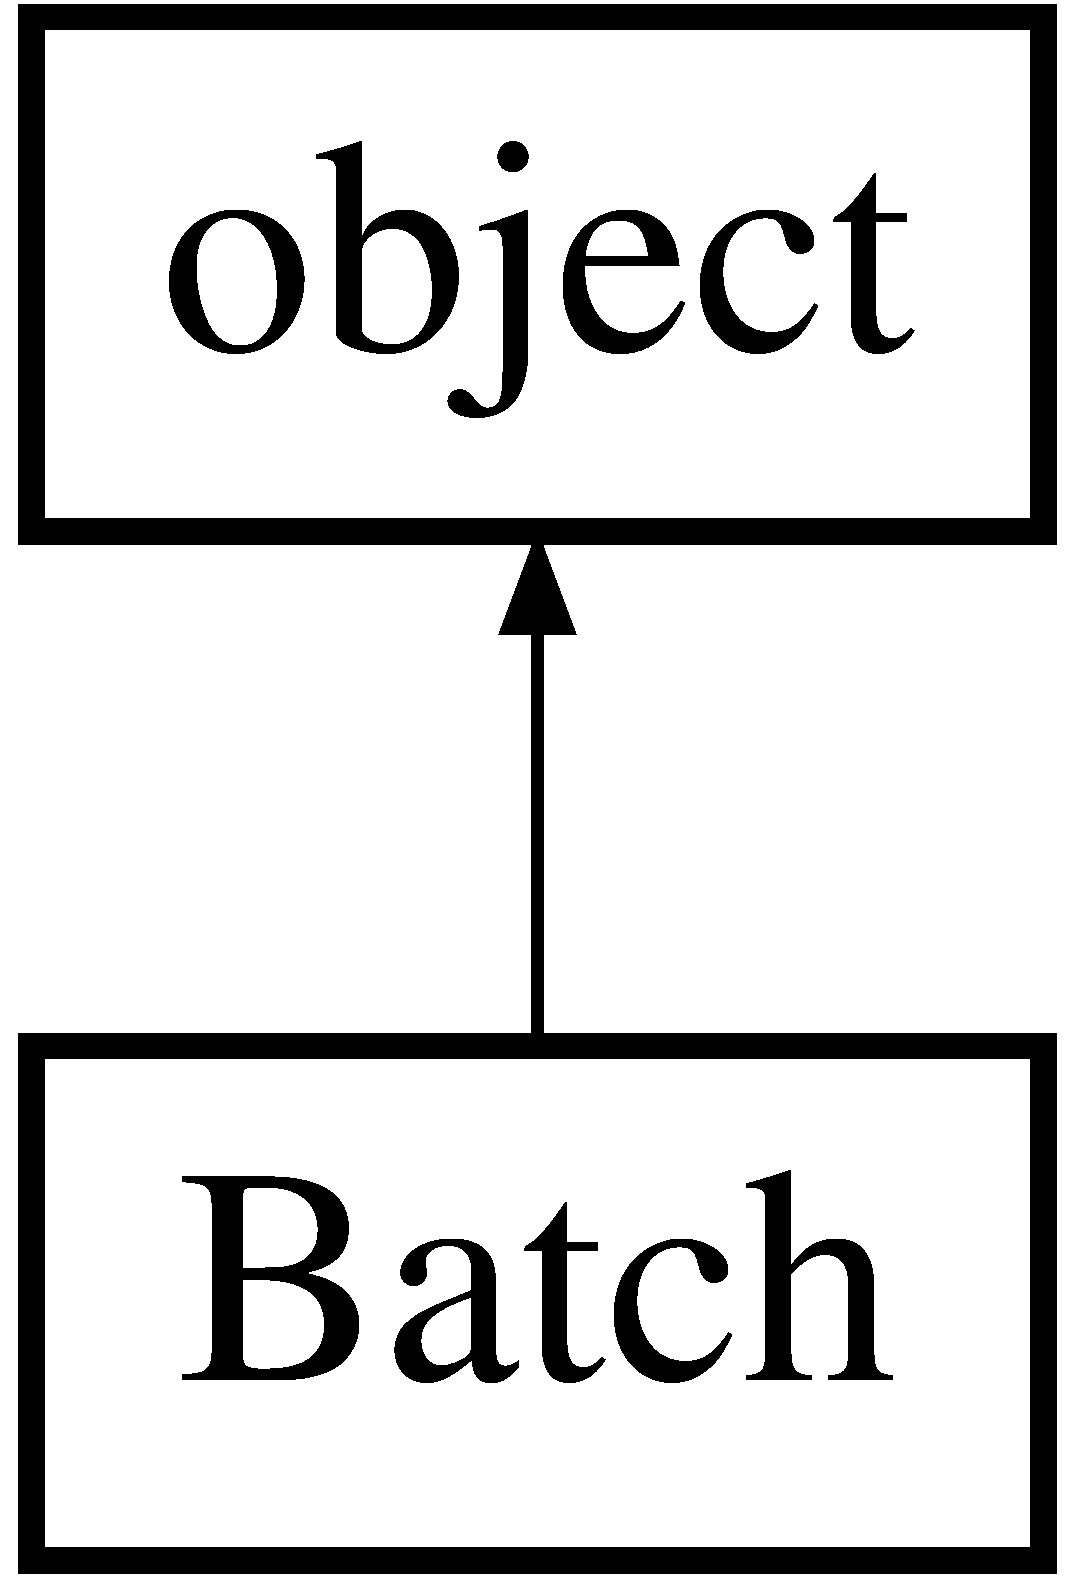
\includegraphics[height=2.000000cm]{classopenbu_1_1nax_1_1functions_1_1_batch}
\end{center}
\end{figure}
\doxysubsection*{Public Member Functions}
\doxysubsection*{Private Attributes}


The documentation for this class was generated from the following file\+:\begin{DoxyCompactItemize}
\item 
nax/functions.\+py\end{DoxyCompactItemize}

\hypertarget{classopenbu_1_1cell_1_1_cell}{}\doxysection{Cell Class Reference}
\label{classopenbu_1_1cell_1_1_cell}\index{Cell@{Cell}}
Inheritance diagram for Cell\+:\begin{figure}[H]
\begin{center}
\leavevmode
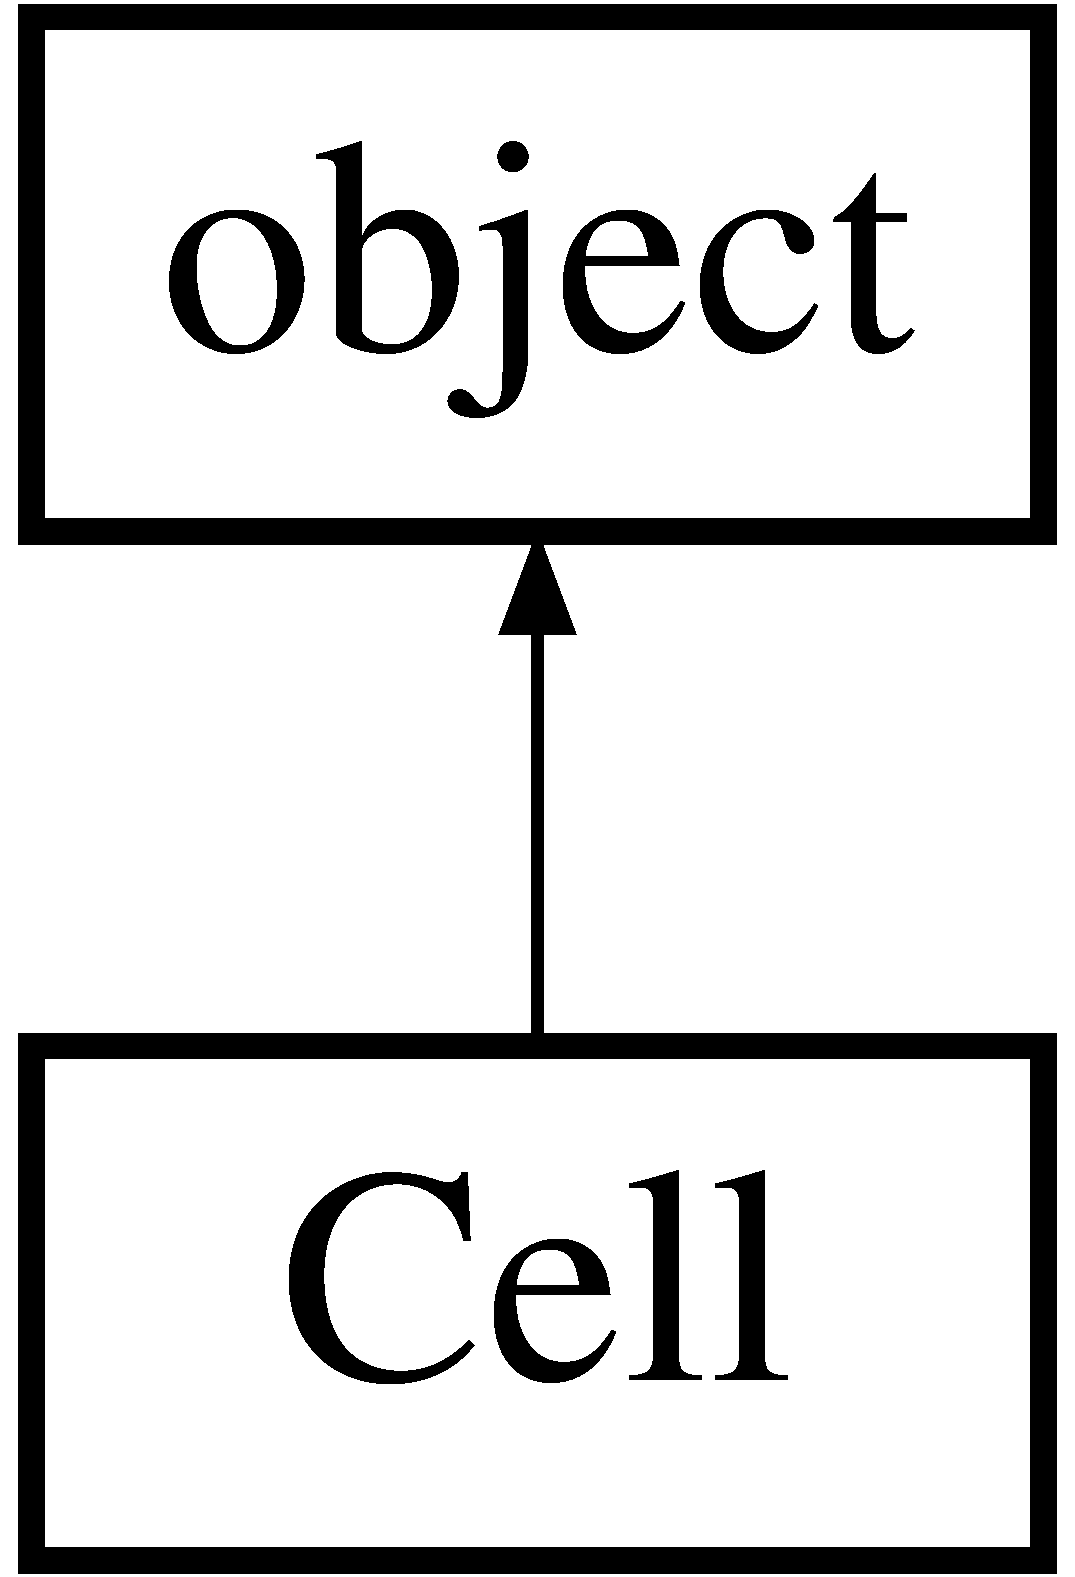
\includegraphics[height=2.000000cm]{classopenbu_1_1cell_1_1_cell}
\end{center}
\end{figure}
\doxysubsection*{Public Member Functions}
\doxysubsection*{Public Attributes}
\doxysubsection*{Static Public Attributes}
\doxysubsection*{Private Member Functions}
\doxysubsection*{Private Attributes}
\doxysubsection*{Static Private Attributes}


\doxysubsection{Member Function Documentation}
\mbox{\Hypertarget{classopenbu_1_1cell_1_1_cell_a60241928100db6ecdc4c8c3459506da9}\label{classopenbu_1_1cell_1_1_cell_a60241928100db6ecdc4c8c3459506da9}} 
\index{Cell@{Cell}!bu\_sec\_conv\_factor@{bu\_sec\_conv\_factor}}
\index{bu\_sec\_conv\_factor@{bu\_sec\_conv\_factor}!Cell@{Cell}}
\doxysubsubsection{\texorpdfstring{bu\_sec\_conv\_factor()}{bu\_sec\_conv\_factor()}}
{\footnotesize\ttfamily def bu\+\_\+sec\+\_\+conv\+\_\+factor (\begin{DoxyParamCaption}\item[{}]{self }\end{DoxyParamCaption})}

\begin{DoxyVerb}Returns the absolute values of the decay constant of the nuclide\end{DoxyVerb}
 \mbox{\Hypertarget{classopenbu_1_1cell_1_1_cell_a50ae19f4fbadad51e8a4d676c4d9866b}\label{classopenbu_1_1cell_1_1_cell_a50ae19f4fbadad51e8a4d676c4d9866b}} 
\index{Cell@{Cell}!ihm@{ihm}}
\index{ihm@{ihm}!Cell@{Cell}}
\doxysubsubsection{\texorpdfstring{ihm()}{ihm()}}
{\footnotesize\ttfamily def ihm (\begin{DoxyParamCaption}\item[{}]{self }\end{DoxyParamCaption})}

\begin{DoxyVerb}Returns the absolute values of the decay constant of the nuclide\end{DoxyVerb}
 

The documentation for this class was generated from the following file\+:\begin{DoxyCompactItemize}
\item 
cell.\+py\end{DoxyCompactItemize}

\hypertarget{classopenbu_1_1system_1_1_cell__name__not__found}{}\section{Cell\+\_\+name\+\_\+not\+\_\+found Class Reference}
\label{classopenbu_1_1system_1_1_cell__name__not__found}\index{Cell\+\_\+name\+\_\+not\+\_\+found@{Cell\+\_\+name\+\_\+not\+\_\+found}}
Inheritance diagram for Cell\+\_\+name\+\_\+not\+\_\+found\+:\begin{figure}[H]
\begin{center}
\leavevmode
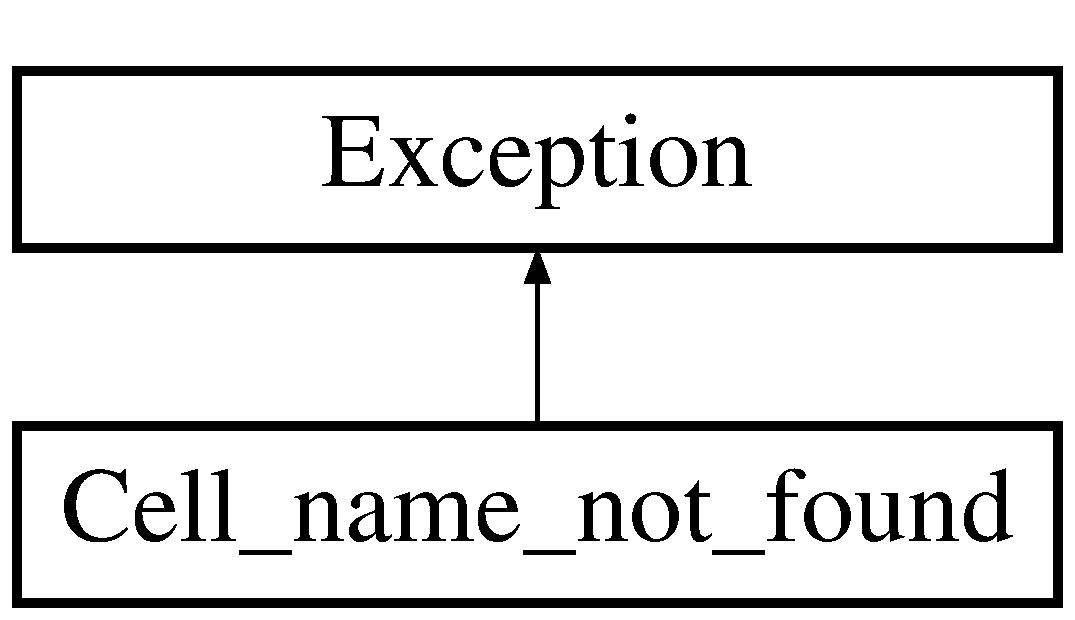
\includegraphics[height=2.000000cm]{classopenbu_1_1system_1_1_cell__name__not__found}
\end{center}
\end{figure}


The documentation for this class was generated from the following file\+:\begin{DoxyCompactItemize}
\item 
/\+Users/mouginot/work/app/\+Open\+B\+U/openbu/\mbox{\hyperlink{system_8py}{system.\+py}}\end{DoxyCompactItemize}

\hypertarget{classopenbu_1_1couple_1_1couple__openmc_1_1_couple__openmc}{}\section{Couple\+\_\+openmc Class Reference}
\label{classopenbu_1_1couple_1_1couple__openmc_1_1_couple__openmc}\index{Couple\+\_\+openmc@{Couple\+\_\+openmc}}
Inheritance diagram for Couple\+\_\+openmc\+:\begin{figure}[H]
\begin{center}
\leavevmode
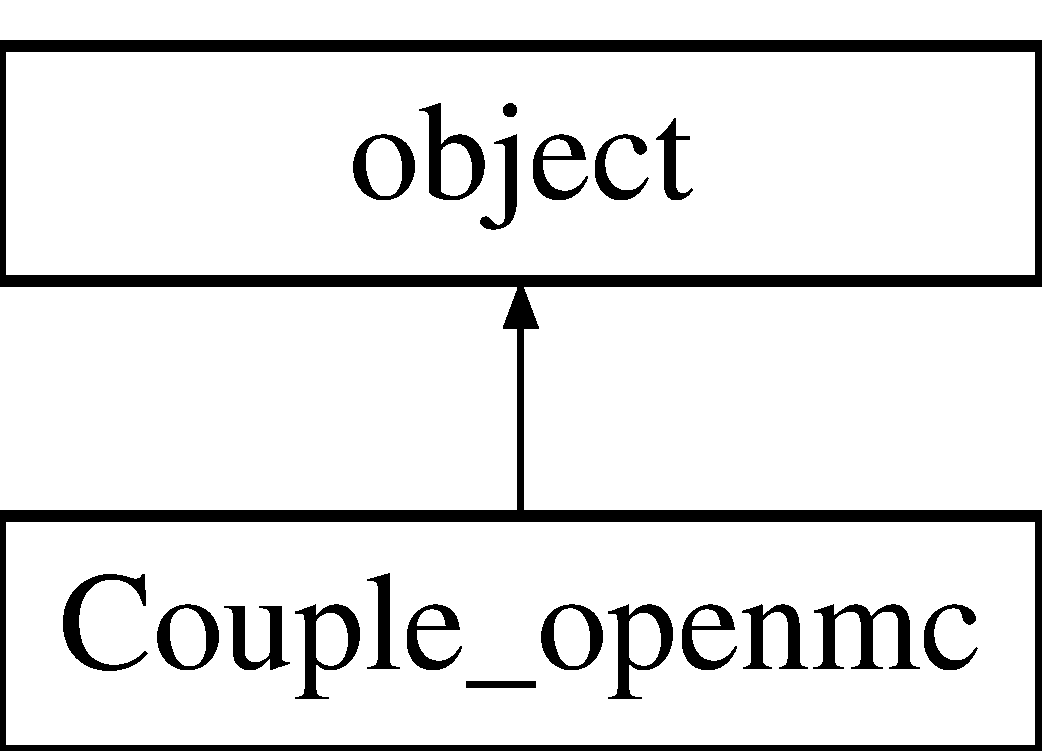
\includegraphics[height=2.000000cm]{classopenbu_1_1couple_1_1couple__openmc_1_1_couple__openmc}
\end{center}
\end{figure}
\subsection*{Public Member Functions}
\subsection*{Public Attributes}
\subsection*{Static Public Attributes}
\subsection*{Private Member Functions}
\subsection*{Private Attributes}


\subsection{Constructor \& Destructor Documentation}
\mbox{\Hypertarget{classopenbu_1_1couple_1_1couple__openmc_1_1_couple__openmc_adf43c036ad3b3850d41894aa20f4bd55}\label{classopenbu_1_1couple_1_1couple__openmc_1_1_couple__openmc_adf43c036ad3b3850d41894aa20f4bd55}} 
\index{openbu\+::couple\+::couple\+\_\+openmc\+::\+Couple\+\_\+openmc@{openbu\+::couple\+::couple\+\_\+openmc\+::\+Couple\+\_\+openmc}!\+\_\+\+\_\+init\+\_\+\+\_\+@{\+\_\+\+\_\+init\+\_\+\+\_\+}}
\index{\+\_\+\+\_\+init\+\_\+\+\_\+@{\+\_\+\+\_\+init\+\_\+\+\_\+}!openbu\+::couple\+::couple\+\_\+openmc\+::\+Couple\+\_\+openmc@{openbu\+::couple\+::couple\+\_\+openmc\+::\+Couple\+\_\+openmc}}
\subsubsection{\texorpdfstring{\+\_\+\+\_\+init\+\_\+\+\_\+()}{\_\_init\_\_()}}
{\footnotesize\ttfamily def \+\_\+\+\_\+init\+\_\+\+\_\+ (\begin{DoxyParamCaption}\item[{}]{self,  }\item[{}]{M\+C\+\_\+input\+\_\+path = {\ttfamily None},  }\item[{}]{xs\+\_\+mode = {\ttfamily \textquotesingle{}no~constant~lib\textquotesingle{}},  }\item[{}]{M\+PI = {\ttfamily None} }\end{DoxyParamCaption})}



\subsection{Member Function Documentation}
\mbox{\Hypertarget{classopenbu_1_1couple_1_1couple__openmc_1_1_couple__openmc_a2807161cebfc8c9d9811d8ee01fa2b7d}\label{classopenbu_1_1couple_1_1couple__openmc_1_1_couple__openmc_a2807161cebfc8c9d9811d8ee01fa2b7d}} 
\index{openbu\+::couple\+::couple\+\_\+openmc\+::\+Couple\+\_\+openmc@{openbu\+::couple\+::couple\+\_\+openmc\+::\+Couple\+\_\+openmc}!\+\_\+change\+\_\+cell\+\_\+materials@{\+\_\+change\+\_\+cell\+\_\+materials}}
\index{\+\_\+change\+\_\+cell\+\_\+materials@{\+\_\+change\+\_\+cell\+\_\+materials}!openbu\+::couple\+::couple\+\_\+openmc\+::\+Couple\+\_\+openmc@{openbu\+::couple\+::couple\+\_\+openmc\+::\+Couple\+\_\+openmc}}
\subsubsection{\texorpdfstring{\+\_\+change\+\_\+cell\+\_\+materials()}{\_change\_cell\_materials()}}
{\footnotesize\ttfamily def \+\_\+change\+\_\+cell\+\_\+materials (\begin{DoxyParamCaption}\item[{}]{self }\end{DoxyParamCaption})\hspace{0.3cm}{\ttfamily [private]}}

\mbox{\Hypertarget{classopenbu_1_1couple_1_1couple__openmc_1_1_couple__openmc_a3327925f8ff34893baf62d7d53f84ffb}\label{classopenbu_1_1couple_1_1couple__openmc_1_1_couple__openmc_a3327925f8ff34893baf62d7d53f84ffb}} 
\index{openbu\+::couple\+::couple\+\_\+openmc\+::\+Couple\+\_\+openmc@{openbu\+::couple\+::couple\+\_\+openmc\+::\+Couple\+\_\+openmc}!\+\_\+pre\+\_\+run@{\+\_\+pre\+\_\+run}}
\index{\+\_\+pre\+\_\+run@{\+\_\+pre\+\_\+run}!openbu\+::couple\+::couple\+\_\+openmc\+::\+Couple\+\_\+openmc@{openbu\+::couple\+::couple\+\_\+openmc\+::\+Couple\+\_\+openmc}}
\subsubsection{\texorpdfstring{\+\_\+pre\+\_\+run()}{\_pre\_run()}}
{\footnotesize\ttfamily def \+\_\+pre\+\_\+run (\begin{DoxyParamCaption}\item[{}]{self,  }\item[{}]{root\+\_\+cell }\end{DoxyParamCaption})\hspace{0.3cm}{\ttfamily [private]}}

\mbox{\Hypertarget{classopenbu_1_1couple_1_1couple__openmc_1_1_couple__openmc_acf4db72a2d51c96f541893afa86a3719}\label{classopenbu_1_1couple_1_1couple__openmc_1_1_couple__openmc_acf4db72a2d51c96f541893afa86a3719}} 
\index{openbu\+::couple\+::couple\+\_\+openmc\+::\+Couple\+\_\+openmc@{openbu\+::couple\+::couple\+\_\+openmc\+::\+Couple\+\_\+openmc}!\+\_\+read\+\_\+user\+\_\+settings@{\+\_\+read\+\_\+user\+\_\+settings}}
\index{\+\_\+read\+\_\+user\+\_\+settings@{\+\_\+read\+\_\+user\+\_\+settings}!openbu\+::couple\+::couple\+\_\+openmc\+::\+Couple\+\_\+openmc@{openbu\+::couple\+::couple\+\_\+openmc\+::\+Couple\+\_\+openmc}}
\subsubsection{\texorpdfstring{\+\_\+read\+\_\+user\+\_\+settings()}{\_read\_user\_settings()}}
{\footnotesize\ttfamily def \+\_\+read\+\_\+user\+\_\+settings (\begin{DoxyParamCaption}\item[{}]{self }\end{DoxyParamCaption})\hspace{0.3cm}{\ttfamily [private]}}

\mbox{\Hypertarget{classopenbu_1_1couple_1_1couple__openmc_1_1_couple__openmc_abb44be8f5b6e448c469f4751897dcba5}\label{classopenbu_1_1couple_1_1couple__openmc_1_1_couple__openmc_abb44be8f5b6e448c469f4751897dcba5}} 
\index{openbu\+::couple\+::couple\+\_\+openmc\+::\+Couple\+\_\+openmc@{openbu\+::couple\+::couple\+\_\+openmc\+::\+Couple\+\_\+openmc}!\+\_\+set\+\_\+cross\+\_\+sections\+\_\+path@{\+\_\+set\+\_\+cross\+\_\+sections\+\_\+path}}
\index{\+\_\+set\+\_\+cross\+\_\+sections\+\_\+path@{\+\_\+set\+\_\+cross\+\_\+sections\+\_\+path}!openbu\+::couple\+::couple\+\_\+openmc\+::\+Couple\+\_\+openmc@{openbu\+::couple\+::couple\+\_\+openmc\+::\+Couple\+\_\+openmc}}
\subsubsection{\texorpdfstring{\+\_\+set\+\_\+cross\+\_\+sections\+\_\+path()}{\_set\_cross\_sections\_path()}}
{\footnotesize\ttfamily def \+\_\+set\+\_\+cross\+\_\+sections\+\_\+path (\begin{DoxyParamCaption}\item[{}]{self,  }\item[{}]{pre\+\_\+run\+\_\+path }\end{DoxyParamCaption})\hspace{0.3cm}{\ttfamily [private]}}

\mbox{\Hypertarget{classopenbu_1_1couple_1_1couple__openmc_1_1_couple__openmc_a9f67057faef0b35164a7d17a24eebaff}\label{classopenbu_1_1couple_1_1couple__openmc_1_1_couple__openmc_a9f67057faef0b35164a7d17a24eebaff}} 
\index{openbu\+::couple\+::couple\+\_\+openmc\+::\+Couple\+\_\+openmc@{openbu\+::couple\+::couple\+\_\+openmc\+::\+Couple\+\_\+openmc}!\+\_\+set\+\_\+initial\+\_\+summary@{\+\_\+set\+\_\+initial\+\_\+summary}}
\index{\+\_\+set\+\_\+initial\+\_\+summary@{\+\_\+set\+\_\+initial\+\_\+summary}!openbu\+::couple\+::couple\+\_\+openmc\+::\+Couple\+\_\+openmc@{openbu\+::couple\+::couple\+\_\+openmc\+::\+Couple\+\_\+openmc}}
\subsubsection{\texorpdfstring{\+\_\+set\+\_\+initial\+\_\+summary()}{\_set\_initial\_summary()}}
{\footnotesize\ttfamily def \+\_\+set\+\_\+initial\+\_\+summary (\begin{DoxyParamCaption}\item[{}]{self,  }\item[{}]{path = {\ttfamily os.getcwd()} }\end{DoxyParamCaption})\hspace{0.3cm}{\ttfamily [private]}}

\mbox{\Hypertarget{classopenbu_1_1couple_1_1couple__openmc_1_1_couple__openmc_aa59058755f41ba2b0de1b748356e480d}\label{classopenbu_1_1couple_1_1couple__openmc_1_1_couple__openmc_aa59058755f41ba2b0de1b748356e480d}} 
\index{openbu\+::couple\+::couple\+\_\+openmc\+::\+Couple\+\_\+openmc@{openbu\+::couple\+::couple\+\_\+openmc\+::\+Couple\+\_\+openmc}!\+\_\+set\+\_\+kinf@{\+\_\+set\+\_\+kinf}}
\index{\+\_\+set\+\_\+kinf@{\+\_\+set\+\_\+kinf}!openbu\+::couple\+::couple\+\_\+openmc\+::\+Couple\+\_\+openmc@{openbu\+::couple\+::couple\+\_\+openmc\+::\+Couple\+\_\+openmc}}
\subsubsection{\texorpdfstring{\+\_\+set\+\_\+kinf()}{\_set\_kinf()}}
{\footnotesize\ttfamily def \+\_\+set\+\_\+kinf (\begin{DoxyParamCaption}\item[{}]{self }\end{DoxyParamCaption})\hspace{0.3cm}{\ttfamily [private]}}

\mbox{\Hypertarget{classopenbu_1_1couple_1_1couple__openmc_1_1_couple__openmc_a484f34b7e4eceac67c32eff27a97d39e}\label{classopenbu_1_1couple_1_1couple__openmc_1_1_couple__openmc_a484f34b7e4eceac67c32eff27a97d39e}} 
\index{openbu\+::couple\+::couple\+\_\+openmc\+::\+Couple\+\_\+openmc@{openbu\+::couple\+::couple\+\_\+openmc\+::\+Couple\+\_\+openmc}!\+\_\+set\+\_\+root\+\_\+cell@{\+\_\+set\+\_\+root\+\_\+cell}}
\index{\+\_\+set\+\_\+root\+\_\+cell@{\+\_\+set\+\_\+root\+\_\+cell}!openbu\+::couple\+::couple\+\_\+openmc\+::\+Couple\+\_\+openmc@{openbu\+::couple\+::couple\+\_\+openmc\+::\+Couple\+\_\+openmc}}
\subsubsection{\texorpdfstring{\+\_\+set\+\_\+root\+\_\+cell()}{\_set\_root\_cell()}}
{\footnotesize\ttfamily def \+\_\+set\+\_\+root\+\_\+cell (\begin{DoxyParamCaption}\item[{}]{self,  }\item[{}]{root\+\_\+cell\+\_\+name }\end{DoxyParamCaption})\hspace{0.3cm}{\ttfamily [private]}}

\mbox{\Hypertarget{classopenbu_1_1couple_1_1couple__openmc_1_1_couple__openmc_ae9625e393903a346dc9d684fdf192edb}\label{classopenbu_1_1couple_1_1couple__openmc_1_1_couple__openmc_ae9625e393903a346dc9d684fdf192edb}} 
\index{openbu\+::couple\+::couple\+\_\+openmc\+::\+Couple\+\_\+openmc@{openbu\+::couple\+::couple\+\_\+openmc\+::\+Couple\+\_\+openmc}!\+\_\+set\+\_\+statepoint@{\+\_\+set\+\_\+statepoint}}
\index{\+\_\+set\+\_\+statepoint@{\+\_\+set\+\_\+statepoint}!openbu\+::couple\+::couple\+\_\+openmc\+::\+Couple\+\_\+openmc@{openbu\+::couple\+::couple\+\_\+openmc\+::\+Couple\+\_\+openmc}}
\subsubsection{\texorpdfstring{\+\_\+set\+\_\+statepoint()}{\_set\_statepoint()}}
{\footnotesize\ttfamily def \+\_\+set\+\_\+statepoint (\begin{DoxyParamCaption}\item[{}]{self,  }\item[{}]{path = {\ttfamily os.getcwd()} }\end{DoxyParamCaption})\hspace{0.3cm}{\ttfamily [private]}}

\mbox{\Hypertarget{classopenbu_1_1couple_1_1couple__openmc_1_1_couple__openmc_a4956616a2a93a4106d31b765439b9ab7}\label{classopenbu_1_1couple_1_1couple__openmc_1_1_couple__openmc_a4956616a2a93a4106d31b765439b9ab7}} 
\index{openbu\+::couple\+::couple\+\_\+openmc\+::\+Couple\+\_\+openmc@{openbu\+::couple\+::couple\+\_\+openmc\+::\+Couple\+\_\+openmc}!\+\_\+set\+\_\+updated\+\_\+summary@{\+\_\+set\+\_\+updated\+\_\+summary}}
\index{\+\_\+set\+\_\+updated\+\_\+summary@{\+\_\+set\+\_\+updated\+\_\+summary}!openbu\+::couple\+::couple\+\_\+openmc\+::\+Couple\+\_\+openmc@{openbu\+::couple\+::couple\+\_\+openmc\+::\+Couple\+\_\+openmc}}
\subsubsection{\texorpdfstring{\+\_\+set\+\_\+updated\+\_\+summary()}{\_set\_updated\_summary()}}
{\footnotesize\ttfamily def \+\_\+set\+\_\+updated\+\_\+summary (\begin{DoxyParamCaption}\item[{}]{self,  }\item[{}]{path = {\ttfamily os.getcwd()} }\end{DoxyParamCaption})\hspace{0.3cm}{\ttfamily [private]}}

\mbox{\Hypertarget{classopenbu_1_1couple_1_1couple__openmc_1_1_couple__openmc_ac6a7964c7f1c353377b2c4dadc5f50a1}\label{classopenbu_1_1couple_1_1couple__openmc_1_1_couple__openmc_ac6a7964c7f1c353377b2c4dadc5f50a1}} 
\index{openbu\+::couple\+::couple\+\_\+openmc\+::\+Couple\+\_\+openmc@{openbu\+::couple\+::couple\+\_\+openmc\+::\+Couple\+\_\+openmc}!add\+\_\+zero\+\_\+dens\+\_\+nuclides@{add\+\_\+zero\+\_\+dens\+\_\+nuclides}}
\index{add\+\_\+zero\+\_\+dens\+\_\+nuclides@{add\+\_\+zero\+\_\+dens\+\_\+nuclides}!openbu\+::couple\+::couple\+\_\+openmc\+::\+Couple\+\_\+openmc@{openbu\+::couple\+::couple\+\_\+openmc\+::\+Couple\+\_\+openmc}}
\subsubsection{\texorpdfstring{add\+\_\+zero\+\_\+dens\+\_\+nuclides()}{add\_zero\_dens\_nuclides()}}
{\footnotesize\ttfamily def add\+\_\+zero\+\_\+dens\+\_\+nuclides (\begin{DoxyParamCaption}\item[{}]{self,  }\item[{}]{cell }\end{DoxyParamCaption})}

\mbox{\Hypertarget{classopenbu_1_1couple_1_1couple__openmc_1_1_couple__openmc_aee8e543a1329dd01ede1e96434b89412}\label{classopenbu_1_1couple_1_1couple__openmc_1_1_couple__openmc_aee8e543a1329dd01ede1e96434b89412}} 
\index{openbu\+::couple\+::couple\+\_\+openmc\+::\+Couple\+\_\+openmc@{openbu\+::couple\+::couple\+\_\+openmc\+::\+Couple\+\_\+openmc}!batches@{batches}}
\index{batches@{batches}!openbu\+::couple\+::couple\+\_\+openmc\+::\+Couple\+\_\+openmc@{openbu\+::couple\+::couple\+\_\+openmc\+::\+Couple\+\_\+openmc}}
\subsubsection{\texorpdfstring{batches()}{batches()}\hspace{0.1cm}{\footnotesize\ttfamily [1/2]}}
{\footnotesize\ttfamily def batches (\begin{DoxyParamCaption}\item[{}]{self }\end{DoxyParamCaption})}

\mbox{\Hypertarget{classopenbu_1_1couple_1_1couple__openmc_1_1_couple__openmc_ab44c2a368eef406c7d2c712a57bbc807}\label{classopenbu_1_1couple_1_1couple__openmc_1_1_couple__openmc_ab44c2a368eef406c7d2c712a57bbc807}} 
\index{openbu\+::couple\+::couple\+\_\+openmc\+::\+Couple\+\_\+openmc@{openbu\+::couple\+::couple\+\_\+openmc\+::\+Couple\+\_\+openmc}!batches@{batches}}
\index{batches@{batches}!openbu\+::couple\+::couple\+\_\+openmc\+::\+Couple\+\_\+openmc@{openbu\+::couple\+::couple\+\_\+openmc\+::\+Couple\+\_\+openmc}}
\subsubsection{\texorpdfstring{batches()}{batches()}\hspace{0.1cm}{\footnotesize\ttfamily [2/2]}}
{\footnotesize\ttfamily def batches (\begin{DoxyParamCaption}\item[{}]{self,  }\item[{}]{batches }\end{DoxyParamCaption})}

\mbox{\Hypertarget{classopenbu_1_1couple_1_1couple__openmc_1_1_couple__openmc_aa488db59629eb4dccde6e0c71edeb2d4}\label{classopenbu_1_1couple_1_1couple__openmc_1_1_couple__openmc_aa488db59629eb4dccde6e0c71edeb2d4}} 
\index{openbu\+::couple\+::couple\+\_\+openmc\+::\+Couple\+\_\+openmc@{openbu\+::couple\+::couple\+\_\+openmc\+::\+Couple\+\_\+openmc}!bounding\+\_\+box@{bounding\+\_\+box}}
\index{bounding\+\_\+box@{bounding\+\_\+box}!openbu\+::couple\+::couple\+\_\+openmc\+::\+Couple\+\_\+openmc@{openbu\+::couple\+::couple\+\_\+openmc\+::\+Couple\+\_\+openmc}}
\subsubsection{\texorpdfstring{bounding\+\_\+box()}{bounding\_box()}}
{\footnotesize\ttfamily def bounding\+\_\+box (\begin{DoxyParamCaption}\item[{}]{self }\end{DoxyParamCaption})}

\mbox{\Hypertarget{classopenbu_1_1couple_1_1couple__openmc_1_1_couple__openmc_a5968b12da4d1097f8c5309aaf43ad278}\label{classopenbu_1_1couple_1_1couple__openmc_1_1_couple__openmc_a5968b12da4d1097f8c5309aaf43ad278}} 
\index{openbu\+::couple\+::couple\+\_\+openmc\+::\+Couple\+\_\+openmc@{openbu\+::couple\+::couple\+\_\+openmc\+::\+Couple\+\_\+openmc}!burn@{burn}}
\index{burn@{burn}!openbu\+::couple\+::couple\+\_\+openmc\+::\+Couple\+\_\+openmc@{openbu\+::couple\+::couple\+\_\+openmc\+::\+Couple\+\_\+openmc}}
\subsubsection{\texorpdfstring{burn()}{burn()}}
{\footnotesize\ttfamily def burn (\begin{DoxyParamCaption}\item[{}]{self }\end{DoxyParamCaption})}

\mbox{\Hypertarget{classopenbu_1_1couple_1_1couple__openmc_1_1_couple__openmc_adc4ee3a13db3358ffdd3d69492377e74}\label{classopenbu_1_1couple_1_1couple__openmc_1_1_couple__openmc_adc4ee3a13db3358ffdd3d69492377e74}} 
\index{openbu\+::couple\+::couple\+\_\+openmc\+::\+Couple\+\_\+openmc@{openbu\+::couple\+::couple\+\_\+openmc\+::\+Couple\+\_\+openmc}!copy\+\_\+\+M\+C\+\_\+files@{copy\+\_\+\+M\+C\+\_\+files}}
\index{copy\+\_\+\+M\+C\+\_\+files@{copy\+\_\+\+M\+C\+\_\+files}!openbu\+::couple\+::couple\+\_\+openmc\+::\+Couple\+\_\+openmc@{openbu\+::couple\+::couple\+\_\+openmc\+::\+Couple\+\_\+openmc}}
\subsubsection{\texorpdfstring{copy\+\_\+\+M\+C\+\_\+files()}{copy\_MC\_files()}}
{\footnotesize\ttfamily def copy\+\_\+\+M\+C\+\_\+files (\begin{DoxyParamCaption}\item[{}]{self,  }\item[{}]{s }\end{DoxyParamCaption})}

\mbox{\Hypertarget{classopenbu_1_1couple_1_1couple__openmc_1_1_couple__openmc_a1b61b8a8e7322d2b0a30da7d5c9c971b}\label{classopenbu_1_1couple_1_1couple__openmc_1_1_couple__openmc_a1b61b8a8e7322d2b0a30da7d5c9c971b}} 
\index{openbu\+::couple\+::couple\+\_\+openmc\+::\+Couple\+\_\+openmc@{openbu\+::couple\+::couple\+\_\+openmc\+::\+Couple\+\_\+openmc}!copy\+\_\+user\+\_\+input@{copy\+\_\+user\+\_\+input}}
\index{copy\+\_\+user\+\_\+input@{copy\+\_\+user\+\_\+input}!openbu\+::couple\+::couple\+\_\+openmc\+::\+Couple\+\_\+openmc@{openbu\+::couple\+::couple\+\_\+openmc\+::\+Couple\+\_\+openmc}}
\subsubsection{\texorpdfstring{copy\+\_\+user\+\_\+input()}{copy\_user\_input()}}
{\footnotesize\ttfamily def copy\+\_\+user\+\_\+input (\begin{DoxyParamCaption}\item[{}]{self }\end{DoxyParamCaption})}

\mbox{\Hypertarget{classopenbu_1_1couple_1_1couple__openmc_1_1_couple__openmc_a828e2a249e1882bf8cddb58796cfe16d}\label{classopenbu_1_1couple_1_1couple__openmc_1_1_couple__openmc_a828e2a249e1882bf8cddb58796cfe16d}} 
\index{openbu\+::couple\+::couple\+\_\+openmc\+::\+Couple\+\_\+openmc@{openbu\+::couple\+::couple\+\_\+openmc\+::\+Couple\+\_\+openmc}!export\+\_\+geometry\+\_\+to\+\_\+xml@{export\+\_\+geometry\+\_\+to\+\_\+xml}}
\index{export\+\_\+geometry\+\_\+to\+\_\+xml@{export\+\_\+geometry\+\_\+to\+\_\+xml}!openbu\+::couple\+::couple\+\_\+openmc\+::\+Couple\+\_\+openmc@{openbu\+::couple\+::couple\+\_\+openmc\+::\+Couple\+\_\+openmc}}
\subsubsection{\texorpdfstring{export\+\_\+geometry\+\_\+to\+\_\+xml()}{export\_geometry\_to\_xml()}}
{\footnotesize\ttfamily def export\+\_\+geometry\+\_\+to\+\_\+xml (\begin{DoxyParamCaption}\item[{}]{self }\end{DoxyParamCaption})}

\mbox{\Hypertarget{classopenbu_1_1couple_1_1couple__openmc_1_1_couple__openmc_ab0f5e73d13112cb5e1d16c32add9c698}\label{classopenbu_1_1couple_1_1couple__openmc_1_1_couple__openmc_ab0f5e73d13112cb5e1d16c32add9c698}} 
\index{openbu\+::couple\+::couple\+\_\+openmc\+::\+Couple\+\_\+openmc@{openbu\+::couple\+::couple\+\_\+openmc\+::\+Couple\+\_\+openmc}!export\+\_\+material\+\_\+to\+\_\+xml@{export\+\_\+material\+\_\+to\+\_\+xml}}
\index{export\+\_\+material\+\_\+to\+\_\+xml@{export\+\_\+material\+\_\+to\+\_\+xml}!openbu\+::couple\+::couple\+\_\+openmc\+::\+Couple\+\_\+openmc@{openbu\+::couple\+::couple\+\_\+openmc\+::\+Couple\+\_\+openmc}}
\subsubsection{\texorpdfstring{export\+\_\+material\+\_\+to\+\_\+xml()}{export\_material\_to\_xml()}}
{\footnotesize\ttfamily def export\+\_\+material\+\_\+to\+\_\+xml (\begin{DoxyParamCaption}\item[{}]{self }\end{DoxyParamCaption})}

\mbox{\Hypertarget{classopenbu_1_1couple_1_1couple__openmc_1_1_couple__openmc_a947e7cc8a90a2a4efa9944c84e5f0323}\label{classopenbu_1_1couple_1_1couple__openmc_1_1_couple__openmc_a947e7cc8a90a2a4efa9944c84e5f0323}} 
\index{openbu\+::couple\+::couple\+\_\+openmc\+::\+Couple\+\_\+openmc@{openbu\+::couple\+::couple\+\_\+openmc\+::\+Couple\+\_\+openmc}!export\+\_\+settings\+\_\+to\+\_\+xml@{export\+\_\+settings\+\_\+to\+\_\+xml}}
\index{export\+\_\+settings\+\_\+to\+\_\+xml@{export\+\_\+settings\+\_\+to\+\_\+xml}!openbu\+::couple\+::couple\+\_\+openmc\+::\+Couple\+\_\+openmc@{openbu\+::couple\+::couple\+\_\+openmc\+::\+Couple\+\_\+openmc}}
\subsubsection{\texorpdfstring{export\+\_\+settings\+\_\+to\+\_\+xml()}{export\_settings\_to\_xml()}}
{\footnotesize\ttfamily def export\+\_\+settings\+\_\+to\+\_\+xml (\begin{DoxyParamCaption}\item[{}]{self }\end{DoxyParamCaption})}

\mbox{\Hypertarget{classopenbu_1_1couple_1_1couple__openmc_1_1_couple__openmc_ab93dec4678af3338259e4abe79b31c6d}\label{classopenbu_1_1couple_1_1couple__openmc_1_1_couple__openmc_ab93dec4678af3338259e4abe79b31c6d}} 
\index{openbu\+::couple\+::couple\+\_\+openmc\+::\+Couple\+\_\+openmc@{openbu\+::couple\+::couple\+\_\+openmc\+::\+Couple\+\_\+openmc}!export\+\_\+tallies\+\_\+to\+\_\+xml@{export\+\_\+tallies\+\_\+to\+\_\+xml}}
\index{export\+\_\+tallies\+\_\+to\+\_\+xml@{export\+\_\+tallies\+\_\+to\+\_\+xml}!openbu\+::couple\+::couple\+\_\+openmc\+::\+Couple\+\_\+openmc@{openbu\+::couple\+::couple\+\_\+openmc\+::\+Couple\+\_\+openmc}}
\subsubsection{\texorpdfstring{export\+\_\+tallies\+\_\+to\+\_\+xml()}{export\_tallies\_to\_xml()}}
{\footnotesize\ttfamily def export\+\_\+tallies\+\_\+to\+\_\+xml (\begin{DoxyParamCaption}\item[{}]{self }\end{DoxyParamCaption})}

\mbox{\Hypertarget{classopenbu_1_1couple_1_1couple__openmc_1_1_couple__openmc_a3171ea6d58bef26700680e0fa2f2643c}\label{classopenbu_1_1couple_1_1couple__openmc_1_1_couple__openmc_a3171ea6d58bef26700680e0fa2f2643c}} 
\index{openbu\+::couple\+::couple\+\_\+openmc\+::\+Couple\+\_\+openmc@{openbu\+::couple\+::couple\+\_\+openmc\+::\+Couple\+\_\+openmc}!gen\+\_\+user\+\_\+input\+\_\+folder@{gen\+\_\+user\+\_\+input\+\_\+folder}}
\index{gen\+\_\+user\+\_\+input\+\_\+folder@{gen\+\_\+user\+\_\+input\+\_\+folder}!openbu\+::couple\+::couple\+\_\+openmc\+::\+Couple\+\_\+openmc@{openbu\+::couple\+::couple\+\_\+openmc\+::\+Couple\+\_\+openmc}}
\subsubsection{\texorpdfstring{gen\+\_\+user\+\_\+input\+\_\+folder()}{gen\_user\_input\_folder()}}
{\footnotesize\ttfamily def gen\+\_\+user\+\_\+input\+\_\+folder (\begin{DoxyParamCaption}\item[{}]{self }\end{DoxyParamCaption})}

\mbox{\Hypertarget{classopenbu_1_1couple_1_1couple__openmc_1_1_couple__openmc_ac271eb1deae1f744a01e8b1a057369d5}\label{classopenbu_1_1couple_1_1couple__openmc_1_1_couple__openmc_ac271eb1deae1f744a01e8b1a057369d5}} 
\index{openbu\+::couple\+::couple\+\_\+openmc\+::\+Couple\+\_\+openmc@{openbu\+::couple\+::couple\+\_\+openmc\+::\+Couple\+\_\+openmc}!get\+\_\+all\+\_\+nucl\+\_\+rxn\+\_\+tally@{get\+\_\+all\+\_\+nucl\+\_\+rxn\+\_\+tally}}
\index{get\+\_\+all\+\_\+nucl\+\_\+rxn\+\_\+tally@{get\+\_\+all\+\_\+nucl\+\_\+rxn\+\_\+tally}!openbu\+::couple\+::couple\+\_\+openmc\+::\+Couple\+\_\+openmc@{openbu\+::couple\+::couple\+\_\+openmc\+::\+Couple\+\_\+openmc}}
\subsubsection{\texorpdfstring{get\+\_\+all\+\_\+nucl\+\_\+rxn\+\_\+tally()}{get\_all\_nucl\_rxn\_tally()}}
{\footnotesize\ttfamily def get\+\_\+all\+\_\+nucl\+\_\+rxn\+\_\+tally (\begin{DoxyParamCaption}\item[{}]{self,  }\item[{}]{bucell }\end{DoxyParamCaption})}

\mbox{\Hypertarget{classopenbu_1_1couple_1_1couple__openmc_1_1_couple__openmc_ac3455eb5524078caf131880d2acb90da}\label{classopenbu_1_1couple_1_1couple__openmc_1_1_couple__openmc_ac3455eb5524078caf131880d2acb90da}} 
\index{openbu\+::couple\+::couple\+\_\+openmc\+::\+Couple\+\_\+openmc@{openbu\+::couple\+::couple\+\_\+openmc\+::\+Couple\+\_\+openmc}!get\+\_\+bucell\+\_\+from\+\_\+cell@{get\+\_\+bucell\+\_\+from\+\_\+cell}}
\index{get\+\_\+bucell\+\_\+from\+\_\+cell@{get\+\_\+bucell\+\_\+from\+\_\+cell}!openbu\+::couple\+::couple\+\_\+openmc\+::\+Couple\+\_\+openmc@{openbu\+::couple\+::couple\+\_\+openmc\+::\+Couple\+\_\+openmc}}
\subsubsection{\texorpdfstring{get\+\_\+bucell\+\_\+from\+\_\+cell()}{get\_bucell\_from\_cell()}}
{\footnotesize\ttfamily def get\+\_\+bucell\+\_\+from\+\_\+cell (\begin{DoxyParamCaption}\item[{}]{self }\end{DoxyParamCaption})}

\mbox{\Hypertarget{classopenbu_1_1couple_1_1couple__openmc_1_1_couple__openmc_ad4720dcbea2a2ee736df2befd86ae244}\label{classopenbu_1_1couple_1_1couple__openmc_1_1_couple__openmc_ad4720dcbea2a2ee736df2befd86ae244}} 
\index{openbu\+::couple\+::couple\+\_\+openmc\+::\+Couple\+\_\+openmc@{openbu\+::couple\+::couple\+\_\+openmc\+::\+Couple\+\_\+openmc}!get\+\_\+flux\+\_\+spectrum\+\_\+tally@{get\+\_\+flux\+\_\+spectrum\+\_\+tally}}
\index{get\+\_\+flux\+\_\+spectrum\+\_\+tally@{get\+\_\+flux\+\_\+spectrum\+\_\+tally}!openbu\+::couple\+::couple\+\_\+openmc\+::\+Couple\+\_\+openmc@{openbu\+::couple\+::couple\+\_\+openmc\+::\+Couple\+\_\+openmc}}
\subsubsection{\texorpdfstring{get\+\_\+flux\+\_\+spectrum\+\_\+tally()}{get\_flux\_spectrum\_tally()}}
{\footnotesize\ttfamily def get\+\_\+flux\+\_\+spectrum\+\_\+tally (\begin{DoxyParamCaption}\item[{}]{self,  }\item[{}]{bucell }\end{DoxyParamCaption})}

\mbox{\Hypertarget{classopenbu_1_1couple_1_1couple__openmc_1_1_couple__openmc_a1aced28963235c39892bfb7eb025dd74}\label{classopenbu_1_1couple_1_1couple__openmc_1_1_couple__openmc_a1aced28963235c39892bfb7eb025dd74}} 
\index{openbu\+::couple\+::couple\+\_\+openmc\+::\+Couple\+\_\+openmc@{openbu\+::couple\+::couple\+\_\+openmc\+::\+Couple\+\_\+openmc}!get\+\_\+flux\+\_\+tally@{get\+\_\+flux\+\_\+tally}}
\index{get\+\_\+flux\+\_\+tally@{get\+\_\+flux\+\_\+tally}!openbu\+::couple\+::couple\+\_\+openmc\+::\+Couple\+\_\+openmc@{openbu\+::couple\+::couple\+\_\+openmc\+::\+Couple\+\_\+openmc}}
\subsubsection{\texorpdfstring{get\+\_\+flux\+\_\+tally()}{get\_flux\_tally()}}
{\footnotesize\ttfamily def get\+\_\+flux\+\_\+tally (\begin{DoxyParamCaption}\item[{}]{self,  }\item[{}]{bucell }\end{DoxyParamCaption})}

\mbox{\Hypertarget{classopenbu_1_1couple_1_1couple__openmc_1_1_couple__openmc_a27a2ccd2322a747e248cb8c953b20d13}\label{classopenbu_1_1couple_1_1couple__openmc_1_1_couple__openmc_a27a2ccd2322a747e248cb8c953b20d13}} 
\index{openbu\+::couple\+::couple\+\_\+openmc\+::\+Couple\+\_\+openmc@{openbu\+::couple\+::couple\+\_\+openmc\+::\+Couple\+\_\+openmc}!get\+\_\+nucl\+\_\+to\+\_\+be\+\_\+tallied@{get\+\_\+nucl\+\_\+to\+\_\+be\+\_\+tallied}}
\index{get\+\_\+nucl\+\_\+to\+\_\+be\+\_\+tallied@{get\+\_\+nucl\+\_\+to\+\_\+be\+\_\+tallied}!openbu\+::couple\+::couple\+\_\+openmc\+::\+Couple\+\_\+openmc@{openbu\+::couple\+::couple\+\_\+openmc\+::\+Couple\+\_\+openmc}}
\subsubsection{\texorpdfstring{get\+\_\+nucl\+\_\+to\+\_\+be\+\_\+tallied()}{get\_nucl\_to\_be\_tallied()}}
{\footnotesize\ttfamily def get\+\_\+nucl\+\_\+to\+\_\+be\+\_\+tallied (\begin{DoxyParamCaption}\item[{}]{self,  }\item[{}]{bucell }\end{DoxyParamCaption})}

\mbox{\Hypertarget{classopenbu_1_1couple_1_1couple__openmc_1_1_couple__openmc_a6aa7288e7a8ac6a95fa650bfc866c0b0}\label{classopenbu_1_1couple_1_1couple__openmc_1_1_couple__openmc_a6aa7288e7a8ac6a95fa650bfc866c0b0}} 
\index{openbu\+::couple\+::couple\+\_\+openmc\+::\+Couple\+\_\+openmc@{openbu\+::couple\+::couple\+\_\+openmc\+::\+Couple\+\_\+openmc}!import\+\_\+openmc@{import\+\_\+openmc}}
\index{import\+\_\+openmc@{import\+\_\+openmc}!openbu\+::couple\+::couple\+\_\+openmc\+::\+Couple\+\_\+openmc@{openbu\+::couple\+::couple\+\_\+openmc\+::\+Couple\+\_\+openmc}}
\subsubsection{\texorpdfstring{import\+\_\+openmc()}{import\_openmc()}}
{\footnotesize\ttfamily def import\+\_\+openmc (\begin{DoxyParamCaption}\item[{}]{self,  }\item[{}]{root\+\_\+cell }\end{DoxyParamCaption})}

\mbox{\Hypertarget{classopenbu_1_1couple_1_1couple__openmc_1_1_couple__openmc_ac27a2578faf8d6c48276ebfd5713d434}\label{classopenbu_1_1couple_1_1couple__openmc_1_1_couple__openmc_ac27a2578faf8d6c48276ebfd5713d434}} 
\index{openbu\+::couple\+::couple\+\_\+openmc\+::\+Couple\+\_\+openmc@{openbu\+::couple\+::couple\+\_\+openmc\+::\+Couple\+\_\+openmc}!inactive@{inactive}}
\index{inactive@{inactive}!openbu\+::couple\+::couple\+\_\+openmc\+::\+Couple\+\_\+openmc@{openbu\+::couple\+::couple\+\_\+openmc\+::\+Couple\+\_\+openmc}}
\subsubsection{\texorpdfstring{inactive()}{inactive()}\hspace{0.1cm}{\footnotesize\ttfamily [1/2]}}
{\footnotesize\ttfamily def inactive (\begin{DoxyParamCaption}\item[{}]{self }\end{DoxyParamCaption})}

\mbox{\Hypertarget{classopenbu_1_1couple_1_1couple__openmc_1_1_couple__openmc_a06a298d260381fee76297a4b97f22216}\label{classopenbu_1_1couple_1_1couple__openmc_1_1_couple__openmc_a06a298d260381fee76297a4b97f22216}} 
\index{openbu\+::couple\+::couple\+\_\+openmc\+::\+Couple\+\_\+openmc@{openbu\+::couple\+::couple\+\_\+openmc\+::\+Couple\+\_\+openmc}!inactive@{inactive}}
\index{inactive@{inactive}!openbu\+::couple\+::couple\+\_\+openmc\+::\+Couple\+\_\+openmc@{openbu\+::couple\+::couple\+\_\+openmc\+::\+Couple\+\_\+openmc}}
\subsubsection{\texorpdfstring{inactive()}{inactive()}\hspace{0.1cm}{\footnotesize\ttfamily [2/2]}}
{\footnotesize\ttfamily def inactive (\begin{DoxyParamCaption}\item[{}]{self,  }\item[{}]{inactive }\end{DoxyParamCaption})}

\mbox{\Hypertarget{classopenbu_1_1couple_1_1couple__openmc_1_1_couple__openmc_a1ff9fde4ab3c74a422841342606f3366}\label{classopenbu_1_1couple_1_1couple__openmc_1_1_couple__openmc_a1ff9fde4ab3c74a422841342606f3366}} 
\index{openbu\+::couple\+::couple\+\_\+openmc\+::\+Couple\+\_\+openmc@{openbu\+::couple\+::couple\+\_\+openmc\+::\+Couple\+\_\+openmc}!init\+\_\+nucl\+\_\+dict@{init\+\_\+nucl\+\_\+dict}}
\index{init\+\_\+nucl\+\_\+dict@{init\+\_\+nucl\+\_\+dict}!openbu\+::couple\+::couple\+\_\+openmc\+::\+Couple\+\_\+openmc@{openbu\+::couple\+::couple\+\_\+openmc\+::\+Couple\+\_\+openmc}}
\subsubsection{\texorpdfstring{init\+\_\+nucl\+\_\+dict()}{init\_nucl\_dict()}}
{\footnotesize\ttfamily def init\+\_\+nucl\+\_\+dict (\begin{DoxyParamCaption}\item[{}]{self }\end{DoxyParamCaption})}

\mbox{\Hypertarget{classopenbu_1_1couple_1_1couple__openmc_1_1_couple__openmc_a7e79cbc7e5ac1cbb4ab61dd44cc52b76}\label{classopenbu_1_1couple_1_1couple__openmc_1_1_couple__openmc_a7e79cbc7e5ac1cbb4ab61dd44cc52b76}} 
\index{openbu\+::couple\+::couple\+\_\+openmc\+::\+Couple\+\_\+openmc@{openbu\+::couple\+::couple\+\_\+openmc\+::\+Couple\+\_\+openmc}!initial\+\_\+couple\+\_\+step\+\_\+normalization@{initial\+\_\+couple\+\_\+step\+\_\+normalization}}
\index{initial\+\_\+couple\+\_\+step\+\_\+normalization@{initial\+\_\+couple\+\_\+step\+\_\+normalization}!openbu\+::couple\+::couple\+\_\+openmc\+::\+Couple\+\_\+openmc@{openbu\+::couple\+::couple\+\_\+openmc\+::\+Couple\+\_\+openmc}}
\subsubsection{\texorpdfstring{initial\+\_\+couple\+\_\+step\+\_\+normalization()}{initial\_couple\_step\_normalization()}}
{\footnotesize\ttfamily def initial\+\_\+couple\+\_\+step\+\_\+normalization (\begin{DoxyParamCaption}\item[{}]{self,  }\item[{}]{norma\+\_\+mode }\end{DoxyParamCaption})}

\mbox{\Hypertarget{classopenbu_1_1couple_1_1couple__openmc_1_1_couple__openmc_abe2fb31ba3167373c6c2c9fa5d7ab0c5}\label{classopenbu_1_1couple_1_1couple__openmc_1_1_couple__openmc_abe2fb31ba3167373c6c2c9fa5d7ab0c5}} 
\index{openbu\+::couple\+::couple\+\_\+openmc\+::\+Couple\+\_\+openmc@{openbu\+::couple\+::couple\+\_\+openmc\+::\+Couple\+\_\+openmc}!initial\+\_\+summary@{initial\+\_\+summary}}
\index{initial\+\_\+summary@{initial\+\_\+summary}!openbu\+::couple\+::couple\+\_\+openmc\+::\+Couple\+\_\+openmc@{openbu\+::couple\+::couple\+\_\+openmc\+::\+Couple\+\_\+openmc}}
\subsubsection{\texorpdfstring{initial\+\_\+summary()}{initial\_summary()}}
{\footnotesize\ttfamily def initial\+\_\+summary (\begin{DoxyParamCaption}\item[{}]{self }\end{DoxyParamCaption})}

\mbox{\Hypertarget{classopenbu_1_1couple_1_1couple__openmc_1_1_couple__openmc_a8e21db711ac4c3dde4d6ac4625b6aab3}\label{classopenbu_1_1couple_1_1couple__openmc_1_1_couple__openmc_a8e21db711ac4c3dde4d6ac4625b6aab3}} 
\index{openbu\+::couple\+::couple\+\_\+openmc\+::\+Couple\+\_\+openmc@{openbu\+::couple\+::couple\+\_\+openmc\+::\+Couple\+\_\+openmc}!materials@{materials}}
\index{materials@{materials}!openbu\+::couple\+::couple\+\_\+openmc\+::\+Couple\+\_\+openmc@{openbu\+::couple\+::couple\+\_\+openmc\+::\+Couple\+\_\+openmc}}
\subsubsection{\texorpdfstring{materials()}{materials()}}
{\footnotesize\ttfamily def materials (\begin{DoxyParamCaption}\item[{}]{self }\end{DoxyParamCaption})}

\mbox{\Hypertarget{classopenbu_1_1couple_1_1couple__openmc_1_1_couple__openmc_a492dece220622b292df514db5cffab61}\label{classopenbu_1_1couple_1_1couple__openmc_1_1_couple__openmc_a492dece220622b292df514db5cffab61}} 
\index{openbu\+::couple\+::couple\+\_\+openmc\+::\+Couple\+\_\+openmc@{openbu\+::couple\+::couple\+\_\+openmc\+::\+Couple\+\_\+openmc}!M\+C\+\_\+input\+\_\+path@{M\+C\+\_\+input\+\_\+path}}
\index{M\+C\+\_\+input\+\_\+path@{M\+C\+\_\+input\+\_\+path}!openbu\+::couple\+::couple\+\_\+openmc\+::\+Couple\+\_\+openmc@{openbu\+::couple\+::couple\+\_\+openmc\+::\+Couple\+\_\+openmc}}
\subsubsection{\texorpdfstring{M\+C\+\_\+input\+\_\+path()}{MC\_input\_path()}}
{\footnotesize\ttfamily def M\+C\+\_\+input\+\_\+path (\begin{DoxyParamCaption}\item[{}]{self }\end{DoxyParamCaption})}

\mbox{\Hypertarget{classopenbu_1_1couple_1_1couple__openmc_1_1_couple__openmc_a3784d088659e77a796c3ffc60b139237}\label{classopenbu_1_1couple_1_1couple__openmc_1_1_couple__openmc_a3784d088659e77a796c3ffc60b139237}} 
\index{openbu\+::couple\+::couple\+\_\+openmc\+::\+Couple\+\_\+openmc@{openbu\+::couple\+::couple\+\_\+openmc\+::\+Couple\+\_\+openmc}!M\+C\+\_\+\+X\+S\+\_\+nucl\+\_\+list@{M\+C\+\_\+\+X\+S\+\_\+nucl\+\_\+list}}
\index{M\+C\+\_\+\+X\+S\+\_\+nucl\+\_\+list@{M\+C\+\_\+\+X\+S\+\_\+nucl\+\_\+list}!openbu\+::couple\+::couple\+\_\+openmc\+::\+Couple\+\_\+openmc@{openbu\+::couple\+::couple\+\_\+openmc\+::\+Couple\+\_\+openmc}}
\subsubsection{\texorpdfstring{M\+C\+\_\+\+X\+S\+\_\+nucl\+\_\+list()}{MC\_XS\_nucl\_list()}\hspace{0.1cm}{\footnotesize\ttfamily [1/2]}}
{\footnotesize\ttfamily def M\+C\+\_\+\+X\+S\+\_\+nucl\+\_\+list (\begin{DoxyParamCaption}\item[{}]{self }\end{DoxyParamCaption})}

\mbox{\Hypertarget{classopenbu_1_1couple_1_1couple__openmc_1_1_couple__openmc_ad0cbaf683d4d93d4e30b876a3eebda61}\label{classopenbu_1_1couple_1_1couple__openmc_1_1_couple__openmc_ad0cbaf683d4d93d4e30b876a3eebda61}} 
\index{openbu\+::couple\+::couple\+\_\+openmc\+::\+Couple\+\_\+openmc@{openbu\+::couple\+::couple\+\_\+openmc\+::\+Couple\+\_\+openmc}!M\+C\+\_\+\+X\+S\+\_\+nucl\+\_\+list@{M\+C\+\_\+\+X\+S\+\_\+nucl\+\_\+list}}
\index{M\+C\+\_\+\+X\+S\+\_\+nucl\+\_\+list@{M\+C\+\_\+\+X\+S\+\_\+nucl\+\_\+list}!openbu\+::couple\+::couple\+\_\+openmc\+::\+Couple\+\_\+openmc@{openbu\+::couple\+::couple\+\_\+openmc\+::\+Couple\+\_\+openmc}}
\subsubsection{\texorpdfstring{M\+C\+\_\+\+X\+S\+\_\+nucl\+\_\+list()}{MC\_XS\_nucl\_list()}\hspace{0.1cm}{\footnotesize\ttfamily [2/2]}}
{\footnotesize\ttfamily def M\+C\+\_\+\+X\+S\+\_\+nucl\+\_\+list (\begin{DoxyParamCaption}\item[{}]{self,  }\item[{}]{M\+C\+\_\+\+X\+S\+\_\+nucl\+\_\+list }\end{DoxyParamCaption})}

\mbox{\Hypertarget{classopenbu_1_1couple_1_1couple__openmc_1_1_couple__openmc_a7be3cbf7a51d054301cc1fc250db0b5e}\label{classopenbu_1_1couple_1_1couple__openmc_1_1_couple__openmc_a7be3cbf7a51d054301cc1fc250db0b5e}} 
\index{openbu\+::couple\+::couple\+\_\+openmc\+::\+Couple\+\_\+openmc@{openbu\+::couple\+::couple\+\_\+openmc\+::\+Couple\+\_\+openmc}!M\+PI@{M\+PI}}
\index{M\+PI@{M\+PI}!openbu\+::couple\+::couple\+\_\+openmc\+::\+Couple\+\_\+openmc@{openbu\+::couple\+::couple\+\_\+openmc\+::\+Couple\+\_\+openmc}}
\subsubsection{\texorpdfstring{M\+P\+I()}{MPI()}}
{\footnotesize\ttfamily def M\+PI (\begin{DoxyParamCaption}\item[{}]{self }\end{DoxyParamCaption})}

\mbox{\Hypertarget{classopenbu_1_1couple_1_1couple__openmc_1_1_couple__openmc_afc348d3ad268d95dcca18adf222837ca}\label{classopenbu_1_1couple_1_1couple__openmc_1_1_couple__openmc_afc348d3ad268d95dcca18adf222837ca}} 
\index{openbu\+::couple\+::couple\+\_\+openmc\+::\+Couple\+\_\+openmc@{openbu\+::couple\+::couple\+\_\+openmc\+::\+Couple\+\_\+openmc}!no\+\_\+decay@{no\+\_\+decay}}
\index{no\+\_\+decay@{no\+\_\+decay}!openbu\+::couple\+::couple\+\_\+openmc\+::\+Couple\+\_\+openmc@{openbu\+::couple\+::couple\+\_\+openmc\+::\+Couple\+\_\+openmc}}
\subsubsection{\texorpdfstring{no\+\_\+decay()}{no\_decay()}}
{\footnotesize\ttfamily def no\+\_\+decay (\begin{DoxyParamCaption}\item[{}]{self }\end{DoxyParamCaption})}

\mbox{\Hypertarget{classopenbu_1_1couple_1_1couple__openmc_1_1_couple__openmc_ab7b32fbfd4abb3ecc5f4a4a8bce45c6a}\label{classopenbu_1_1couple_1_1couple__openmc_1_1_couple__openmc_ab7b32fbfd4abb3ecc5f4a4a8bce45c6a}} 
\index{openbu\+::couple\+::couple\+\_\+openmc\+::\+Couple\+\_\+openmc@{openbu\+::couple\+::couple\+\_\+openmc\+::\+Couple\+\_\+openmc}!nucl\+\_\+list\+\_\+dict@{nucl\+\_\+list\+\_\+dict}}
\index{nucl\+\_\+list\+\_\+dict@{nucl\+\_\+list\+\_\+dict}!openbu\+::couple\+::couple\+\_\+openmc\+::\+Couple\+\_\+openmc@{openbu\+::couple\+::couple\+\_\+openmc\+::\+Couple\+\_\+openmc}}
\subsubsection{\texorpdfstring{nucl\+\_\+list\+\_\+dict()}{nucl\_list\_dict()}}
{\footnotesize\ttfamily def nucl\+\_\+list\+\_\+dict (\begin{DoxyParamCaption}\item[{}]{self }\end{DoxyParamCaption})}

\mbox{\Hypertarget{classopenbu_1_1couple_1_1couple__openmc_1_1_couple__openmc_a65c15fc2939e02be841bfb81c447a105}\label{classopenbu_1_1couple_1_1couple__openmc_1_1_couple__openmc_a65c15fc2939e02be841bfb81c447a105}} 
\index{openbu\+::couple\+::couple\+\_\+openmc\+::\+Couple\+\_\+openmc@{openbu\+::couple\+::couple\+\_\+openmc\+::\+Couple\+\_\+openmc}!openmc\+\_\+bin\+\_\+path@{openmc\+\_\+bin\+\_\+path}}
\index{openmc\+\_\+bin\+\_\+path@{openmc\+\_\+bin\+\_\+path}!openbu\+::couple\+::couple\+\_\+openmc\+::\+Couple\+\_\+openmc@{openbu\+::couple\+::couple\+\_\+openmc\+::\+Couple\+\_\+openmc}}
\subsubsection{\texorpdfstring{openmc\+\_\+bin\+\_\+path()}{openmc\_bin\_path()}\hspace{0.1cm}{\footnotesize\ttfamily [1/2]}}
{\footnotesize\ttfamily def openmc\+\_\+bin\+\_\+path (\begin{DoxyParamCaption}\item[{}]{self }\end{DoxyParamCaption})}

\mbox{\Hypertarget{classopenbu_1_1couple_1_1couple__openmc_1_1_couple__openmc_aadbbaaee764ed9659ed2dc2f9e354901}\label{classopenbu_1_1couple_1_1couple__openmc_1_1_couple__openmc_aadbbaaee764ed9659ed2dc2f9e354901}} 
\index{openbu\+::couple\+::couple\+\_\+openmc\+::\+Couple\+\_\+openmc@{openbu\+::couple\+::couple\+\_\+openmc\+::\+Couple\+\_\+openmc}!openmc\+\_\+bin\+\_\+path@{openmc\+\_\+bin\+\_\+path}}
\index{openmc\+\_\+bin\+\_\+path@{openmc\+\_\+bin\+\_\+path}!openbu\+::couple\+::couple\+\_\+openmc\+::\+Couple\+\_\+openmc@{openbu\+::couple\+::couple\+\_\+openmc\+::\+Couple\+\_\+openmc}}
\subsubsection{\texorpdfstring{openmc\+\_\+bin\+\_\+path()}{openmc\_bin\_path()}\hspace{0.1cm}{\footnotesize\ttfamily [2/2]}}
{\footnotesize\ttfamily def openmc\+\_\+bin\+\_\+path (\begin{DoxyParamCaption}\item[{}]{self,  }\item[{}]{openmc\+\_\+bin\+\_\+path }\end{DoxyParamCaption})}

\mbox{\Hypertarget{classopenbu_1_1couple_1_1couple__openmc_1_1_couple__openmc_abf02a0f769a3aabd1bd5fce1859223ec}\label{classopenbu_1_1couple_1_1couple__openmc_1_1_couple__openmc_abf02a0f769a3aabd1bd5fce1859223ec}} 
\index{openbu\+::couple\+::couple\+\_\+openmc\+::\+Couple\+\_\+openmc@{openbu\+::couple\+::couple\+\_\+openmc\+::\+Couple\+\_\+openmc}!particles@{particles}}
\index{particles@{particles}!openbu\+::couple\+::couple\+\_\+openmc\+::\+Couple\+\_\+openmc@{openbu\+::couple\+::couple\+\_\+openmc\+::\+Couple\+\_\+openmc}}
\subsubsection{\texorpdfstring{particles()}{particles()}\hspace{0.1cm}{\footnotesize\ttfamily [1/2]}}
{\footnotesize\ttfamily def particles (\begin{DoxyParamCaption}\item[{}]{self }\end{DoxyParamCaption})}

\mbox{\Hypertarget{classopenbu_1_1couple_1_1couple__openmc_1_1_couple__openmc_a746f4b485013a1e0b0a604be35135040}\label{classopenbu_1_1couple_1_1couple__openmc_1_1_couple__openmc_a746f4b485013a1e0b0a604be35135040}} 
\index{openbu\+::couple\+::couple\+\_\+openmc\+::\+Couple\+\_\+openmc@{openbu\+::couple\+::couple\+\_\+openmc\+::\+Couple\+\_\+openmc}!particles@{particles}}
\index{particles@{particles}!openbu\+::couple\+::couple\+\_\+openmc\+::\+Couple\+\_\+openmc@{openbu\+::couple\+::couple\+\_\+openmc\+::\+Couple\+\_\+openmc}}
\subsubsection{\texorpdfstring{particles()}{particles()}\hspace{0.1cm}{\footnotesize\ttfamily [2/2]}}
{\footnotesize\ttfamily def particles (\begin{DoxyParamCaption}\item[{}]{self,  }\item[{}]{particles }\end{DoxyParamCaption})}

\mbox{\Hypertarget{classopenbu_1_1couple_1_1couple__openmc_1_1_couple__openmc_a2e6fc3693cee9ca38ebae31635ac5583}\label{classopenbu_1_1couple_1_1couple__openmc_1_1_couple__openmc_a2e6fc3693cee9ca38ebae31635ac5583}} 
\index{openbu\+::couple\+::couple\+\_\+openmc\+::\+Couple\+\_\+openmc@{openbu\+::couple\+::couple\+\_\+openmc\+::\+Couple\+\_\+openmc}!pass\+\_\+nuclide\+\_\+densities@{pass\+\_\+nuclide\+\_\+densities}}
\index{pass\+\_\+nuclide\+\_\+densities@{pass\+\_\+nuclide\+\_\+densities}!openbu\+::couple\+::couple\+\_\+openmc\+::\+Couple\+\_\+openmc@{openbu\+::couple\+::couple\+\_\+openmc\+::\+Couple\+\_\+openmc}}
\subsubsection{\texorpdfstring{pass\+\_\+nuclide\+\_\+densities()}{pass\_nuclide\_densities()}}
{\footnotesize\ttfamily def pass\+\_\+nuclide\+\_\+densities (\begin{DoxyParamCaption}\item[{}]{self,  }\item[{}]{cell\+\_\+dict,  }\item[{}]{bucell\+\_\+dict }\end{DoxyParamCaption})}

\mbox{\Hypertarget{classopenbu_1_1couple_1_1couple__openmc_1_1_couple__openmc_a5f2e5eaec6ee4c0fd18ee8b67321e09f}\label{classopenbu_1_1couple_1_1couple__openmc_1_1_couple__openmc_a5f2e5eaec6ee4c0fd18ee8b67321e09f}} 
\index{openbu\+::couple\+::couple\+\_\+openmc\+::\+Couple\+\_\+openmc@{openbu\+::couple\+::couple\+\_\+openmc\+::\+Couple\+\_\+openmc}!pass\+\_\+vol@{pass\+\_\+vol}}
\index{pass\+\_\+vol@{pass\+\_\+vol}!openbu\+::couple\+::couple\+\_\+openmc\+::\+Couple\+\_\+openmc@{openbu\+::couple\+::couple\+\_\+openmc\+::\+Couple\+\_\+openmc}}
\subsubsection{\texorpdfstring{pass\+\_\+vol()}{pass\_vol()}}
{\footnotesize\ttfamily def pass\+\_\+vol (\begin{DoxyParamCaption}\item[{}]{self,  }\item[{}]{cell\+\_\+dict,  }\item[{}]{bucell\+\_\+dict }\end{DoxyParamCaption})}

\mbox{\Hypertarget{classopenbu_1_1couple_1_1couple__openmc_1_1_couple__openmc_ab2fbb5d193f8877b8ab3acf1da98bbb1}\label{classopenbu_1_1couple_1_1couple__openmc_1_1_couple__openmc_ab2fbb5d193f8877b8ab3acf1da98bbb1}} 
\index{openbu\+::couple\+::couple\+\_\+openmc\+::\+Couple\+\_\+openmc@{openbu\+::couple\+::couple\+\_\+openmc\+::\+Couple\+\_\+openmc}!root\+\_\+cell@{root\+\_\+cell}}
\index{root\+\_\+cell@{root\+\_\+cell}!openbu\+::couple\+::couple\+\_\+openmc\+::\+Couple\+\_\+openmc@{openbu\+::couple\+::couple\+\_\+openmc\+::\+Couple\+\_\+openmc}}
\subsubsection{\texorpdfstring{root\+\_\+cell()}{root\_cell()}\hspace{0.1cm}{\footnotesize\ttfamily [1/2]}}
{\footnotesize\ttfamily def root\+\_\+cell (\begin{DoxyParamCaption}\item[{}]{self }\end{DoxyParamCaption})}

\mbox{\Hypertarget{classopenbu_1_1couple_1_1couple__openmc_1_1_couple__openmc_ab2fbb5d193f8877b8ab3acf1da98bbb1}\label{classopenbu_1_1couple_1_1couple__openmc_1_1_couple__openmc_ab2fbb5d193f8877b8ab3acf1da98bbb1}} 
\index{openbu\+::couple\+::couple\+\_\+openmc\+::\+Couple\+\_\+openmc@{openbu\+::couple\+::couple\+\_\+openmc\+::\+Couple\+\_\+openmc}!root\+\_\+cell@{root\+\_\+cell}}
\index{root\+\_\+cell@{root\+\_\+cell}!openbu\+::couple\+::couple\+\_\+openmc\+::\+Couple\+\_\+openmc@{openbu\+::couple\+::couple\+\_\+openmc\+::\+Couple\+\_\+openmc}}
\subsubsection{\texorpdfstring{root\+\_\+cell()}{root\_cell()}\hspace{0.1cm}{\footnotesize\ttfamily [2/2]}}
{\footnotesize\ttfamily def root\+\_\+cell (\begin{DoxyParamCaption}\item[{}]{self }\end{DoxyParamCaption})}

\mbox{\Hypertarget{classopenbu_1_1couple_1_1couple__openmc_1_1_couple__openmc_a045da5fa1ce270ec2e2d5ca3a59370fe}\label{classopenbu_1_1couple_1_1couple__openmc_1_1_couple__openmc_a045da5fa1ce270ec2e2d5ca3a59370fe}} 
\index{openbu\+::couple\+::couple\+\_\+openmc\+::\+Couple\+\_\+openmc@{openbu\+::couple\+::couple\+\_\+openmc\+::\+Couple\+\_\+openmc}!run\+\_\+openmc@{run\+\_\+openmc}}
\index{run\+\_\+openmc@{run\+\_\+openmc}!openbu\+::couple\+::couple\+\_\+openmc\+::\+Couple\+\_\+openmc@{openbu\+::couple\+::couple\+\_\+openmc\+::\+Couple\+\_\+openmc}}
\subsubsection{\texorpdfstring{run\+\_\+openmc()}{run\_openmc()}}
{\footnotesize\ttfamily def run\+\_\+openmc (\begin{DoxyParamCaption}\item[{}]{self }\end{DoxyParamCaption})}

\mbox{\Hypertarget{classopenbu_1_1couple_1_1couple__openmc_1_1_couple__openmc_acbf74409e97046ae5f11d94451fddbc9}\label{classopenbu_1_1couple_1_1couple__openmc_1_1_couple__openmc_acbf74409e97046ae5f11d94451fddbc9}} 
\index{openbu\+::couple\+::couple\+\_\+openmc\+::\+Couple\+\_\+openmc@{openbu\+::couple\+::couple\+\_\+openmc\+::\+Couple\+\_\+openmc}!select\+\_\+bucells@{select\+\_\+bucells}}
\index{select\+\_\+bucells@{select\+\_\+bucells}!openbu\+::couple\+::couple\+\_\+openmc\+::\+Couple\+\_\+openmc@{openbu\+::couple\+::couple\+\_\+openmc\+::\+Couple\+\_\+openmc}}
\subsubsection{\texorpdfstring{select\+\_\+bucells()}{select\_bucells()}}
{\footnotesize\ttfamily def select\+\_\+bucells (\begin{DoxyParamCaption}\item[{}]{self,  }\item[{}]{bucell\+\_\+list }\end{DoxyParamCaption})}

\mbox{\Hypertarget{classopenbu_1_1couple_1_1couple__openmc_1_1_couple__openmc_abccf5c11b2da221a2cf1f948977c4b93}\label{classopenbu_1_1couple_1_1couple__openmc_1_1_couple__openmc_abccf5c11b2da221a2cf1f948977c4b93}} 
\index{openbu\+::couple\+::couple\+\_\+openmc\+::\+Couple\+\_\+openmc@{openbu\+::couple\+::couple\+\_\+openmc\+::\+Couple\+\_\+openmc}!sequence@{sequence}}
\index{sequence@{sequence}!openbu\+::couple\+::couple\+\_\+openmc\+::\+Couple\+\_\+openmc@{openbu\+::couple\+::couple\+\_\+openmc\+::\+Couple\+\_\+openmc}}
\subsubsection{\texorpdfstring{sequence()}{sequence()}\hspace{0.1cm}{\footnotesize\ttfamily [1/2]}}
{\footnotesize\ttfamily def sequence (\begin{DoxyParamCaption}\item[{}]{self }\end{DoxyParamCaption})}

\mbox{\Hypertarget{classopenbu_1_1couple_1_1couple__openmc_1_1_couple__openmc_a722dd4f3dcc143383fdfd84269e4c3d5}\label{classopenbu_1_1couple_1_1couple__openmc_1_1_couple__openmc_a722dd4f3dcc143383fdfd84269e4c3d5}} 
\index{openbu\+::couple\+::couple\+\_\+openmc\+::\+Couple\+\_\+openmc@{openbu\+::couple\+::couple\+\_\+openmc\+::\+Couple\+\_\+openmc}!sequence@{sequence}}
\index{sequence@{sequence}!openbu\+::couple\+::couple\+\_\+openmc\+::\+Couple\+\_\+openmc@{openbu\+::couple\+::couple\+\_\+openmc\+::\+Couple\+\_\+openmc}}
\subsubsection{\texorpdfstring{sequence()}{sequence()}\hspace{0.1cm}{\footnotesize\ttfamily [2/2]}}
{\footnotesize\ttfamily def sequence (\begin{DoxyParamCaption}\item[{}]{self,  }\item[{}]{sequence }\end{DoxyParamCaption})}

\mbox{\Hypertarget{classopenbu_1_1couple_1_1couple__openmc_1_1_couple__openmc_af33a9f9e26dd138f532feb3f93ad9aa3}\label{classopenbu_1_1couple_1_1couple__openmc_1_1_couple__openmc_af33a9f9e26dd138f532feb3f93ad9aa3}} 
\index{openbu\+::couple\+::couple\+\_\+openmc\+::\+Couple\+\_\+openmc@{openbu\+::couple\+::couple\+\_\+openmc\+::\+Couple\+\_\+openmc}!set\+\_\+bounding\+\_\+box@{set\+\_\+bounding\+\_\+box}}
\index{set\+\_\+bounding\+\_\+box@{set\+\_\+bounding\+\_\+box}!openbu\+::couple\+::couple\+\_\+openmc\+::\+Couple\+\_\+openmc@{openbu\+::couple\+::couple\+\_\+openmc\+::\+Couple\+\_\+openmc}}
\subsubsection{\texorpdfstring{set\+\_\+bounding\+\_\+box()}{set\_bounding\_box()}}
{\footnotesize\ttfamily def set\+\_\+bounding\+\_\+box (\begin{DoxyParamCaption}\item[{}]{self,  }\item[{}]{ll,  }\item[{}]{ur }\end{DoxyParamCaption})}

\mbox{\Hypertarget{classopenbu_1_1couple_1_1couple__openmc_1_1_couple__openmc_a7e78297a2d71ac9bf4bb3cfd198a66bb}\label{classopenbu_1_1couple_1_1couple__openmc_1_1_couple__openmc_a7e78297a2d71ac9bf4bb3cfd198a66bb}} 
\index{openbu\+::couple\+::couple\+\_\+openmc\+::\+Couple\+\_\+openmc@{openbu\+::couple\+::couple\+\_\+openmc\+::\+Couple\+\_\+openmc}!set\+\_\+decay\+\_\+from\+\_\+object@{set\+\_\+decay\+\_\+from\+\_\+object}}
\index{set\+\_\+decay\+\_\+from\+\_\+object@{set\+\_\+decay\+\_\+from\+\_\+object}!openbu\+::couple\+::couple\+\_\+openmc\+::\+Couple\+\_\+openmc@{openbu\+::couple\+::couple\+\_\+openmc\+::\+Couple\+\_\+openmc}}
\subsubsection{\texorpdfstring{set\+\_\+decay\+\_\+from\+\_\+object()}{set\_decay\_from\_object()}}
{\footnotesize\ttfamily def set\+\_\+decay\+\_\+from\+\_\+object (\begin{DoxyParamCaption}\item[{}]{self,  }\item[{}]{bucell,  }\item[{}]{object }\end{DoxyParamCaption})}

\mbox{\Hypertarget{classopenbu_1_1couple_1_1couple__openmc_1_1_couple__openmc_abefa1ff54b69eaf78c2faca6a54e23da}\label{classopenbu_1_1couple_1_1couple__openmc_1_1_couple__openmc_abefa1ff54b69eaf78c2faca6a54e23da}} 
\index{openbu\+::couple\+::couple\+\_\+openmc\+::\+Couple\+\_\+openmc@{openbu\+::couple\+::couple\+\_\+openmc\+::\+Couple\+\_\+openmc}!set\+\_\+decay\+\_\+lib@{set\+\_\+decay\+\_\+lib}}
\index{set\+\_\+decay\+\_\+lib@{set\+\_\+decay\+\_\+lib}!openbu\+::couple\+::couple\+\_\+openmc\+::\+Couple\+\_\+openmc@{openbu\+::couple\+::couple\+\_\+openmc\+::\+Couple\+\_\+openmc}}
\subsubsection{\texorpdfstring{set\+\_\+decay\+\_\+lib()}{set\_decay\_lib()}}
{\footnotesize\ttfamily def set\+\_\+decay\+\_\+lib (\begin{DoxyParamCaption}\item[{}]{self,  }\item[{}]{decay\+\_\+lib\+\_\+path }\end{DoxyParamCaption})}

\mbox{\Hypertarget{classopenbu_1_1couple_1_1couple__openmc_1_1_couple__openmc_a88b30ccee58b6fc14842f9bfe720268d}\label{classopenbu_1_1couple_1_1couple__openmc_1_1_couple__openmc_a88b30ccee58b6fc14842f9bfe720268d}} 
\index{openbu\+::couple\+::couple\+\_\+openmc\+::\+Couple\+\_\+openmc@{openbu\+::couple\+::couple\+\_\+openmc\+::\+Couple\+\_\+openmc}!set\+\_\+default\+\_\+decay\+\_\+lib@{set\+\_\+default\+\_\+decay\+\_\+lib}}
\index{set\+\_\+default\+\_\+decay\+\_\+lib@{set\+\_\+default\+\_\+decay\+\_\+lib}!openbu\+::couple\+::couple\+\_\+openmc\+::\+Couple\+\_\+openmc@{openbu\+::couple\+::couple\+\_\+openmc\+::\+Couple\+\_\+openmc}}
\subsubsection{\texorpdfstring{set\+\_\+default\+\_\+decay\+\_\+lib()}{set\_default\_decay\_lib()}}
{\footnotesize\ttfamily def set\+\_\+default\+\_\+decay\+\_\+lib (\begin{DoxyParamCaption}\item[{}]{self }\end{DoxyParamCaption})}

\mbox{\Hypertarget{classopenbu_1_1couple_1_1couple__openmc_1_1_couple__openmc_a63cd11db2aba16b8d95b2dbe225487ac}\label{classopenbu_1_1couple_1_1couple__openmc_1_1_couple__openmc_a63cd11db2aba16b8d95b2dbe225487ac}} 
\index{openbu\+::couple\+::couple\+\_\+openmc\+::\+Couple\+\_\+openmc@{openbu\+::couple\+::couple\+\_\+openmc\+::\+Couple\+\_\+openmc}!set\+\_\+default\+\_\+fy\+\_\+lib@{set\+\_\+default\+\_\+fy\+\_\+lib}}
\index{set\+\_\+default\+\_\+fy\+\_\+lib@{set\+\_\+default\+\_\+fy\+\_\+lib}!openbu\+::couple\+::couple\+\_\+openmc\+::\+Couple\+\_\+openmc@{openbu\+::couple\+::couple\+\_\+openmc\+::\+Couple\+\_\+openmc}}
\subsubsection{\texorpdfstring{set\+\_\+default\+\_\+fy\+\_\+lib()}{set\_default\_fy\_lib()}}
{\footnotesize\ttfamily def set\+\_\+default\+\_\+fy\+\_\+lib (\begin{DoxyParamCaption}\item[{}]{self }\end{DoxyParamCaption})}

\mbox{\Hypertarget{classopenbu_1_1couple_1_1couple__openmc_1_1_couple__openmc_a5984355dcb947dfe85271ea01b90f42e}\label{classopenbu_1_1couple_1_1couple__openmc_1_1_couple__openmc_a5984355dcb947dfe85271ea01b90f42e}} 
\index{openbu\+::couple\+::couple\+\_\+openmc\+::\+Couple\+\_\+openmc@{openbu\+::couple\+::couple\+\_\+openmc\+::\+Couple\+\_\+openmc}!set\+\_\+default\+\_\+xs\+\_\+lib@{set\+\_\+default\+\_\+xs\+\_\+lib}}
\index{set\+\_\+default\+\_\+xs\+\_\+lib@{set\+\_\+default\+\_\+xs\+\_\+lib}!openbu\+::couple\+::couple\+\_\+openmc\+::\+Couple\+\_\+openmc@{openbu\+::couple\+::couple\+\_\+openmc\+::\+Couple\+\_\+openmc}}
\subsubsection{\texorpdfstring{set\+\_\+default\+\_\+xs\+\_\+lib()}{set\_default\_xs\_lib()}}
{\footnotesize\ttfamily def set\+\_\+default\+\_\+xs\+\_\+lib (\begin{DoxyParamCaption}\item[{}]{self }\end{DoxyParamCaption})}

\mbox{\Hypertarget{classopenbu_1_1couple_1_1couple__openmc_1_1_couple__openmc_a45bb21cfd88787d53a1013e94afaa4ca}\label{classopenbu_1_1couple_1_1couple__openmc_1_1_couple__openmc_a45bb21cfd88787d53a1013e94afaa4ca}} 
\index{openbu\+::couple\+::couple\+\_\+openmc\+::\+Couple\+\_\+openmc@{openbu\+::couple\+::couple\+\_\+openmc\+::\+Couple\+\_\+openmc}!set\+\_\+dens\+\_\+to\+\_\+cells@{set\+\_\+dens\+\_\+to\+\_\+cells}}
\index{set\+\_\+dens\+\_\+to\+\_\+cells@{set\+\_\+dens\+\_\+to\+\_\+cells}!openbu\+::couple\+::couple\+\_\+openmc\+::\+Couple\+\_\+openmc@{openbu\+::couple\+::couple\+\_\+openmc\+::\+Couple\+\_\+openmc}}
\subsubsection{\texorpdfstring{set\+\_\+dens\+\_\+to\+\_\+cells()}{set\_dens\_to\_cells()}}
{\footnotesize\ttfamily def set\+\_\+dens\+\_\+to\+\_\+cells (\begin{DoxyParamCaption}\item[{}]{self }\end{DoxyParamCaption})}

\mbox{\Hypertarget{classopenbu_1_1couple_1_1couple__openmc_1_1_couple__openmc_abee36b75c3058b430fbcad4919e80eee}\label{classopenbu_1_1couple_1_1couple__openmc_1_1_couple__openmc_abee36b75c3058b430fbcad4919e80eee}} 
\index{openbu\+::couple\+::couple\+\_\+openmc\+::\+Couple\+\_\+openmc@{openbu\+::couple\+::couple\+\_\+openmc\+::\+Couple\+\_\+openmc}!set\+\_\+fy\+\_\+from\+\_\+object@{set\+\_\+fy\+\_\+from\+\_\+object}}
\index{set\+\_\+fy\+\_\+from\+\_\+object@{set\+\_\+fy\+\_\+from\+\_\+object}!openbu\+::couple\+::couple\+\_\+openmc\+::\+Couple\+\_\+openmc@{openbu\+::couple\+::couple\+\_\+openmc\+::\+Couple\+\_\+openmc}}
\subsubsection{\texorpdfstring{set\+\_\+fy\+\_\+from\+\_\+object()}{set\_fy\_from\_object()}}
{\footnotesize\ttfamily def set\+\_\+fy\+\_\+from\+\_\+object (\begin{DoxyParamCaption}\item[{}]{self,  }\item[{}]{bucell,  }\item[{}]{object }\end{DoxyParamCaption})}

\mbox{\Hypertarget{classopenbu_1_1couple_1_1couple__openmc_1_1_couple__openmc_a7e7f585c25f1fec460b794a08e23d8e1}\label{classopenbu_1_1couple_1_1couple__openmc_1_1_couple__openmc_a7e7f585c25f1fec460b794a08e23d8e1}} 
\index{openbu\+::couple\+::couple\+\_\+openmc\+::\+Couple\+\_\+openmc@{openbu\+::couple\+::couple\+\_\+openmc\+::\+Couple\+\_\+openmc}!set\+\_\+fy\+\_\+lib@{set\+\_\+fy\+\_\+lib}}
\index{set\+\_\+fy\+\_\+lib@{set\+\_\+fy\+\_\+lib}!openbu\+::couple\+::couple\+\_\+openmc\+::\+Couple\+\_\+openmc@{openbu\+::couple\+::couple\+\_\+openmc\+::\+Couple\+\_\+openmc}}
\subsubsection{\texorpdfstring{set\+\_\+fy\+\_\+lib()}{set\_fy\_lib()}}
{\footnotesize\ttfamily def set\+\_\+fy\+\_\+lib (\begin{DoxyParamCaption}\item[{}]{self,  }\item[{}]{fy\+\_\+lib\+\_\+path }\end{DoxyParamCaption})}

\mbox{\Hypertarget{classopenbu_1_1couple_1_1couple__openmc_1_1_couple__openmc_aac68d82c71aea78c2bb204ebc3d012ef}\label{classopenbu_1_1couple_1_1couple__openmc_1_1_couple__openmc_aac68d82c71aea78c2bb204ebc3d012ef}} 
\index{openbu\+::couple\+::couple\+\_\+openmc\+::\+Couple\+\_\+openmc@{openbu\+::couple\+::couple\+\_\+openmc\+::\+Couple\+\_\+openmc}!set\+\_\+init\+\_\+nucl@{set\+\_\+init\+\_\+nucl}}
\index{set\+\_\+init\+\_\+nucl@{set\+\_\+init\+\_\+nucl}!openbu\+::couple\+::couple\+\_\+openmc\+::\+Couple\+\_\+openmc@{openbu\+::couple\+::couple\+\_\+openmc\+::\+Couple\+\_\+openmc}}
\subsubsection{\texorpdfstring{set\+\_\+init\+\_\+nucl()}{set\_init\_nucl()}}
{\footnotesize\ttfamily def set\+\_\+init\+\_\+nucl (\begin{DoxyParamCaption}\item[{}]{self,  }\item[{}]{cell\+\_\+dict,  }\item[{}]{bucell\+\_\+dict }\end{DoxyParamCaption})}

\mbox{\Hypertarget{classopenbu_1_1couple_1_1couple__openmc_1_1_couple__openmc_a133340afdd506430947279af06a651d1}\label{classopenbu_1_1couple_1_1couple__openmc_1_1_couple__openmc_a133340afdd506430947279af06a651d1}} 
\index{openbu\+::couple\+::couple\+\_\+openmc\+::\+Couple\+\_\+openmc@{openbu\+::couple\+::couple\+\_\+openmc\+::\+Couple\+\_\+openmc}!set\+\_\+init\+\_\+nucl\+\_\+dict@{set\+\_\+init\+\_\+nucl\+\_\+dict}}
\index{set\+\_\+init\+\_\+nucl\+\_\+dict@{set\+\_\+init\+\_\+nucl\+\_\+dict}!openbu\+::couple\+::couple\+\_\+openmc\+::\+Couple\+\_\+openmc@{openbu\+::couple\+::couple\+\_\+openmc\+::\+Couple\+\_\+openmc}}
\subsubsection{\texorpdfstring{set\+\_\+init\+\_\+nucl\+\_\+dict()}{set\_init\_nucl\_dict()}}
{\footnotesize\ttfamily def set\+\_\+init\+\_\+nucl\+\_\+dict (\begin{DoxyParamCaption}\item[{}]{self,  }\item[{}]{root\+\_\+cell }\end{DoxyParamCaption})}

\mbox{\Hypertarget{classopenbu_1_1couple_1_1couple__openmc_1_1_couple__openmc_a50662bd61824c9b7f55cc2522b7c1353}\label{classopenbu_1_1couple_1_1couple__openmc_1_1_couple__openmc_a50662bd61824c9b7f55cc2522b7c1353}} 
\index{openbu\+::couple\+::couple\+\_\+openmc\+::\+Couple\+\_\+openmc@{openbu\+::couple\+::couple\+\_\+openmc\+::\+Couple\+\_\+openmc}!set\+\_\+\+M\+C\+\_\+\+X\+S\+\_\+nuc\+\_\+list\+\_\+to\+\_\+bucells@{set\+\_\+\+M\+C\+\_\+\+X\+S\+\_\+nuc\+\_\+list\+\_\+to\+\_\+bucells}}
\index{set\+\_\+\+M\+C\+\_\+\+X\+S\+\_\+nuc\+\_\+list\+\_\+to\+\_\+bucells@{set\+\_\+\+M\+C\+\_\+\+X\+S\+\_\+nuc\+\_\+list\+\_\+to\+\_\+bucells}!openbu\+::couple\+::couple\+\_\+openmc\+::\+Couple\+\_\+openmc@{openbu\+::couple\+::couple\+\_\+openmc\+::\+Couple\+\_\+openmc}}
\subsubsection{\texorpdfstring{set\+\_\+\+M\+C\+\_\+\+X\+S\+\_\+nuc\+\_\+list\+\_\+to\+\_\+bucells()}{set\_MC\_XS\_nuc\_list\_to\_bucells()}}
{\footnotesize\ttfamily def set\+\_\+\+M\+C\+\_\+\+X\+S\+\_\+nuc\+\_\+list\+\_\+to\+\_\+bucells (\begin{DoxyParamCaption}\item[{}]{self }\end{DoxyParamCaption})}

\mbox{\Hypertarget{classopenbu_1_1couple_1_1couple__openmc_1_1_couple__openmc_a4df9419c8ee01a5b677882b676320eb4}\label{classopenbu_1_1couple_1_1couple__openmc_1_1_couple__openmc_a4df9419c8ee01a5b677882b676320eb4}} 
\index{openbu\+::couple\+::couple\+\_\+openmc\+::\+Couple\+\_\+openmc@{openbu\+::couple\+::couple\+\_\+openmc\+::\+Couple\+\_\+openmc}!set\+\_\+\+M\+C\+\_\+\+X\+S\+\_\+nucl\+\_\+list@{set\+\_\+\+M\+C\+\_\+\+X\+S\+\_\+nucl\+\_\+list}}
\index{set\+\_\+\+M\+C\+\_\+\+X\+S\+\_\+nucl\+\_\+list@{set\+\_\+\+M\+C\+\_\+\+X\+S\+\_\+nucl\+\_\+list}!openbu\+::couple\+::couple\+\_\+openmc\+::\+Couple\+\_\+openmc@{openbu\+::couple\+::couple\+\_\+openmc\+::\+Couple\+\_\+openmc}}
\subsubsection{\texorpdfstring{set\+\_\+\+M\+C\+\_\+\+X\+S\+\_\+nucl\+\_\+list()}{set\_MC\_XS\_nucl\_list()}}
{\footnotesize\ttfamily def set\+\_\+\+M\+C\+\_\+\+X\+S\+\_\+nucl\+\_\+list (\begin{DoxyParamCaption}\item[{}]{self }\end{DoxyParamCaption})}

\mbox{\Hypertarget{classopenbu_1_1couple_1_1couple__openmc_1_1_couple__openmc_a7659fa6d27dcebba1a28be484b6b6628}\label{classopenbu_1_1couple_1_1couple__openmc_1_1_couple__openmc_a7659fa6d27dcebba1a28be484b6b6628}} 
\index{openbu\+::couple\+::couple\+\_\+openmc\+::\+Couple\+\_\+openmc@{openbu\+::couple\+::couple\+\_\+openmc\+::\+Couple\+\_\+openmc}!set\+\_\+\+M\+PI@{set\+\_\+\+M\+PI}}
\index{set\+\_\+\+M\+PI@{set\+\_\+\+M\+PI}!openbu\+::couple\+::couple\+\_\+openmc\+::\+Couple\+\_\+openmc@{openbu\+::couple\+::couple\+\_\+openmc\+::\+Couple\+\_\+openmc}}
\subsubsection{\texorpdfstring{set\+\_\+\+M\+P\+I()}{set\_MPI()}}
{\footnotesize\ttfamily def set\+\_\+\+M\+PI (\begin{DoxyParamCaption}\item[{}]{self,  }\item[{}]{execu,  }\item[{}]{tasks }\end{DoxyParamCaption})}

\mbox{\Hypertarget{classopenbu_1_1couple_1_1couple__openmc_1_1_couple__openmc_ac7f38b4f1482bf9b861fa0e1ea75b2f5}\label{classopenbu_1_1couple_1_1couple__openmc_1_1_couple__openmc_ac7f38b4f1482bf9b861fa0e1ea75b2f5}} 
\index{openbu\+::couple\+::couple\+\_\+openmc\+::\+Couple\+\_\+openmc@{openbu\+::couple\+::couple\+\_\+openmc\+::\+Couple\+\_\+openmc}!set\+\_\+root\+\_\+universe@{set\+\_\+root\+\_\+universe}}
\index{set\+\_\+root\+\_\+universe@{set\+\_\+root\+\_\+universe}!openbu\+::couple\+::couple\+\_\+openmc\+::\+Couple\+\_\+openmc@{openbu\+::couple\+::couple\+\_\+openmc\+::\+Couple\+\_\+openmc}}
\subsubsection{\texorpdfstring{set\+\_\+root\+\_\+universe()}{set\_root\_universe()}}
{\footnotesize\ttfamily def set\+\_\+root\+\_\+universe (\begin{DoxyParamCaption}\item[{}]{self }\end{DoxyParamCaption})}

\mbox{\Hypertarget{classopenbu_1_1couple_1_1couple__openmc_1_1_couple__openmc_aaa3f58c453fbbaeb685858ff185e17a7}\label{classopenbu_1_1couple_1_1couple__openmc_1_1_couple__openmc_aaa3f58c453fbbaeb685858ff185e17a7}} 
\index{openbu\+::couple\+::couple\+\_\+openmc\+::\+Couple\+\_\+openmc@{openbu\+::couple\+::couple\+\_\+openmc\+::\+Couple\+\_\+openmc}!set\+\_\+sampled\+\_\+isomeric\+\_\+branching\+\_\+data@{set\+\_\+sampled\+\_\+isomeric\+\_\+branching\+\_\+data}}
\index{set\+\_\+sampled\+\_\+isomeric\+\_\+branching\+\_\+data@{set\+\_\+sampled\+\_\+isomeric\+\_\+branching\+\_\+data}!openbu\+::couple\+::couple\+\_\+openmc\+::\+Couple\+\_\+openmc@{openbu\+::couple\+::couple\+\_\+openmc\+::\+Couple\+\_\+openmc}}
\subsubsection{\texorpdfstring{set\+\_\+sampled\+\_\+isomeric\+\_\+branching\+\_\+data()}{set\_sampled\_isomeric\_branching\_data()}}
{\footnotesize\ttfamily def set\+\_\+sampled\+\_\+isomeric\+\_\+branching\+\_\+data (\begin{DoxyParamCaption}\item[{}]{self }\end{DoxyParamCaption})}

\mbox{\Hypertarget{classopenbu_1_1couple_1_1couple__openmc_1_1_couple__openmc_a2a5271c35e1298787f159d1605537976}\label{classopenbu_1_1couple_1_1couple__openmc_1_1_couple__openmc_a2a5271c35e1298787f159d1605537976}} 
\index{openbu\+::couple\+::couple\+\_\+openmc\+::\+Couple\+\_\+openmc@{openbu\+::couple\+::couple\+\_\+openmc\+::\+Couple\+\_\+openmc}!set\+\_\+sampled\+\_\+ng\+\_\+cross\+\_\+section\+\_\+data@{set\+\_\+sampled\+\_\+ng\+\_\+cross\+\_\+section\+\_\+data}}
\index{set\+\_\+sampled\+\_\+ng\+\_\+cross\+\_\+section\+\_\+data@{set\+\_\+sampled\+\_\+ng\+\_\+cross\+\_\+section\+\_\+data}!openbu\+::couple\+::couple\+\_\+openmc\+::\+Couple\+\_\+openmc@{openbu\+::couple\+::couple\+\_\+openmc\+::\+Couple\+\_\+openmc}}
\subsubsection{\texorpdfstring{set\+\_\+sampled\+\_\+ng\+\_\+cross\+\_\+section\+\_\+data()}{set\_sampled\_ng\_cross\_section\_data()}}
{\footnotesize\ttfamily def set\+\_\+sampled\+\_\+ng\+\_\+cross\+\_\+section\+\_\+data (\begin{DoxyParamCaption}\item[{}]{self }\end{DoxyParamCaption})}

\mbox{\Hypertarget{classopenbu_1_1couple_1_1couple__openmc_1_1_couple__openmc_ae604cb072118c5073801d5c39ac1675b}\label{classopenbu_1_1couple_1_1couple__openmc_1_1_couple__openmc_ae604cb072118c5073801d5c39ac1675b}} 
\index{openbu\+::couple\+::couple\+\_\+openmc\+::\+Couple\+\_\+openmc@{openbu\+::couple\+::couple\+\_\+openmc\+::\+Couple\+\_\+openmc}!set\+\_\+sequence@{set\+\_\+sequence}}
\index{set\+\_\+sequence@{set\+\_\+sequence}!openbu\+::couple\+::couple\+\_\+openmc\+::\+Couple\+\_\+openmc@{openbu\+::couple\+::couple\+\_\+openmc\+::\+Couple\+\_\+openmc}}
\subsubsection{\texorpdfstring{set\+\_\+sequence()}{set\_sequence()}}
{\footnotesize\ttfamily def set\+\_\+sequence (\begin{DoxyParamCaption}\item[{}]{self,  }\item[{}]{sequence }\end{DoxyParamCaption})}

\mbox{\Hypertarget{classopenbu_1_1couple_1_1couple__openmc_1_1_couple__openmc_aa08aee78f4a4f37e2f2bb17851b421cd}\label{classopenbu_1_1couple_1_1couple__openmc_1_1_couple__openmc_aa08aee78f4a4f37e2f2bb17851b421cd}} 
\index{openbu\+::couple\+::couple\+\_\+openmc\+::\+Couple\+\_\+openmc@{openbu\+::couple\+::couple\+\_\+openmc\+::\+Couple\+\_\+openmc}!set\+\_\+settings@{set\+\_\+settings}}
\index{set\+\_\+settings@{set\+\_\+settings}!openbu\+::couple\+::couple\+\_\+openmc\+::\+Couple\+\_\+openmc@{openbu\+::couple\+::couple\+\_\+openmc\+::\+Couple\+\_\+openmc}}
\subsubsection{\texorpdfstring{set\+\_\+settings()}{set\_settings()}}
{\footnotesize\ttfamily def set\+\_\+settings (\begin{DoxyParamCaption}\item[{}]{self,  }\item[{}]{settings,  }\item[{}]{init\+\_\+dist }\end{DoxyParamCaption})}

\mbox{\Hypertarget{classopenbu_1_1couple_1_1couple__openmc_1_1_couple__openmc_ab5f7cb97f85f785c0208d5d176128c4a}\label{classopenbu_1_1couple_1_1couple__openmc_1_1_couple__openmc_ab5f7cb97f85f785c0208d5d176128c4a}} 
\index{openbu\+::couple\+::couple\+\_\+openmc\+::\+Couple\+\_\+openmc@{openbu\+::couple\+::couple\+\_\+openmc\+::\+Couple\+\_\+openmc}!set\+\_\+tallies\+\_\+to\+\_\+bucells@{set\+\_\+tallies\+\_\+to\+\_\+bucells}}
\index{set\+\_\+tallies\+\_\+to\+\_\+bucells@{set\+\_\+tallies\+\_\+to\+\_\+bucells}!openbu\+::couple\+::couple\+\_\+openmc\+::\+Couple\+\_\+openmc@{openbu\+::couple\+::couple\+\_\+openmc\+::\+Couple\+\_\+openmc}}
\subsubsection{\texorpdfstring{set\+\_\+tallies\+\_\+to\+\_\+bucells()}{set\_tallies\_to\_bucells()}}
{\footnotesize\ttfamily def set\+\_\+tallies\+\_\+to\+\_\+bucells (\begin{DoxyParamCaption}\item[{}]{self,  }\item[{}]{s }\end{DoxyParamCaption})}

\mbox{\Hypertarget{classopenbu_1_1couple_1_1couple__openmc_1_1_couple__openmc_a7abe37040cea236777fb72454c42da3d}\label{classopenbu_1_1couple_1_1couple__openmc_1_1_couple__openmc_a7abe37040cea236777fb72454c42da3d}} 
\index{openbu\+::couple\+::couple\+\_\+openmc\+::\+Couple\+\_\+openmc@{openbu\+::couple\+::couple\+\_\+openmc\+::\+Couple\+\_\+openmc}!set\+\_\+vol@{set\+\_\+vol}}
\index{set\+\_\+vol@{set\+\_\+vol}!openbu\+::couple\+::couple\+\_\+openmc\+::\+Couple\+\_\+openmc@{openbu\+::couple\+::couple\+\_\+openmc\+::\+Couple\+\_\+openmc}}
\subsubsection{\texorpdfstring{set\+\_\+vol()}{set\_vol()}}
{\footnotesize\ttfamily def set\+\_\+vol (\begin{DoxyParamCaption}\item[{}]{self,  }\item[{}]{vol\+\_\+dict }\end{DoxyParamCaption})}

\mbox{\Hypertarget{classopenbu_1_1couple_1_1couple__openmc_1_1_couple__openmc_afb2b584a4a38fc501c9dbbc515859e52}\label{classopenbu_1_1couple_1_1couple__openmc_1_1_couple__openmc_afb2b584a4a38fc501c9dbbc515859e52}} 
\index{openbu\+::couple\+::couple\+\_\+openmc\+::\+Couple\+\_\+openmc@{openbu\+::couple\+::couple\+\_\+openmc\+::\+Couple\+\_\+openmc}!set\+\_\+vol\+\_\+to\+\_\+cell@{set\+\_\+vol\+\_\+to\+\_\+cell}}
\index{set\+\_\+vol\+\_\+to\+\_\+cell@{set\+\_\+vol\+\_\+to\+\_\+cell}!openbu\+::couple\+::couple\+\_\+openmc\+::\+Couple\+\_\+openmc@{openbu\+::couple\+::couple\+\_\+openmc\+::\+Couple\+\_\+openmc}}
\subsubsection{\texorpdfstring{set\+\_\+vol\+\_\+to\+\_\+cell()}{set\_vol\_to\_cell()}}
{\footnotesize\ttfamily def set\+\_\+vol\+\_\+to\+\_\+cell (\begin{DoxyParamCaption}\item[{}]{self,  }\item[{}]{vol1,  }\item[{}]{pre\+\_\+run\+\_\+path }\end{DoxyParamCaption})}

\mbox{\Hypertarget{classopenbu_1_1couple_1_1couple__openmc_1_1_couple__openmc_aba319705a8d1a57b70fe1ac790292a55}\label{classopenbu_1_1couple_1_1couple__openmc_1_1_couple__openmc_aba319705a8d1a57b70fe1ac790292a55}} 
\index{openbu\+::couple\+::couple\+\_\+openmc\+::\+Couple\+\_\+openmc@{openbu\+::couple\+::couple\+\_\+openmc\+::\+Couple\+\_\+openmc}!set\+\_\+xs\+\_\+lib@{set\+\_\+xs\+\_\+lib}}
\index{set\+\_\+xs\+\_\+lib@{set\+\_\+xs\+\_\+lib}!openbu\+::couple\+::couple\+\_\+openmc\+::\+Couple\+\_\+openmc@{openbu\+::couple\+::couple\+\_\+openmc\+::\+Couple\+\_\+openmc}}
\subsubsection{\texorpdfstring{set\+\_\+xs\+\_\+lib()}{set\_xs\_lib()}}
{\footnotesize\ttfamily def set\+\_\+xs\+\_\+lib (\begin{DoxyParamCaption}\item[{}]{self,  }\item[{}]{xs\+\_\+lib\+\_\+path }\end{DoxyParamCaption})}

\mbox{\Hypertarget{classopenbu_1_1couple_1_1couple__openmc_1_1_couple__openmc_a49f7090e9a0c52fe1aeda3edcef8e3a4}\label{classopenbu_1_1couple_1_1couple__openmc_1_1_couple__openmc_a49f7090e9a0c52fe1aeda3edcef8e3a4}} 
\index{openbu\+::couple\+::couple\+\_\+openmc\+::\+Couple\+\_\+openmc@{openbu\+::couple\+::couple\+\_\+openmc\+::\+Couple\+\_\+openmc}!settings@{settings}}
\index{settings@{settings}!openbu\+::couple\+::couple\+\_\+openmc\+::\+Couple\+\_\+openmc@{openbu\+::couple\+::couple\+\_\+openmc\+::\+Couple\+\_\+openmc}}
\subsubsection{\texorpdfstring{settings()}{settings()}}
{\footnotesize\ttfamily def settings (\begin{DoxyParamCaption}\item[{}]{self }\end{DoxyParamCaption})}

\mbox{\Hypertarget{classopenbu_1_1couple_1_1couple__openmc_1_1_couple__openmc_af538a1fdd6b6fedece38559210f32e0f}\label{classopenbu_1_1couple_1_1couple__openmc_1_1_couple__openmc_af538a1fdd6b6fedece38559210f32e0f}} 
\index{openbu\+::couple\+::couple\+\_\+openmc\+::\+Couple\+\_\+openmc@{openbu\+::couple\+::couple\+\_\+openmc\+::\+Couple\+\_\+openmc}!statepoint@{statepoint}}
\index{statepoint@{statepoint}!openbu\+::couple\+::couple\+\_\+openmc\+::\+Couple\+\_\+openmc@{openbu\+::couple\+::couple\+\_\+openmc\+::\+Couple\+\_\+openmc}}
\subsubsection{\texorpdfstring{statepoint()}{statepoint()}}
{\footnotesize\ttfamily def statepoint (\begin{DoxyParamCaption}\item[{}]{self }\end{DoxyParamCaption})}

\mbox{\Hypertarget{classopenbu_1_1couple_1_1couple__openmc_1_1_couple__openmc_a026f5c4b8598c2d71ee11f4867700c49}\label{classopenbu_1_1couple_1_1couple__openmc_1_1_couple__openmc_a026f5c4b8598c2d71ee11f4867700c49}} 
\index{openbu\+::couple\+::couple\+\_\+openmc\+::\+Couple\+\_\+openmc@{openbu\+::couple\+::couple\+\_\+openmc\+::\+Couple\+\_\+openmc}!step\+\_\+normalization@{step\+\_\+normalization}}
\index{step\+\_\+normalization@{step\+\_\+normalization}!openbu\+::couple\+::couple\+\_\+openmc\+::\+Couple\+\_\+openmc@{openbu\+::couple\+::couple\+\_\+openmc\+::\+Couple\+\_\+openmc}}
\subsubsection{\texorpdfstring{step\+\_\+normalization()}{step\_normalization()}}
{\footnotesize\ttfamily def step\+\_\+normalization (\begin{DoxyParamCaption}\item[{}]{self,  }\item[{}]{s }\end{DoxyParamCaption})}

\mbox{\Hypertarget{classopenbu_1_1couple_1_1couple__openmc_1_1_couple__openmc_a95e3ae0fb087a5d956cd8916603872e0}\label{classopenbu_1_1couple_1_1couple__openmc_1_1_couple__openmc_a95e3ae0fb087a5d956cd8916603872e0}} 
\index{openbu\+::couple\+::couple\+\_\+openmc\+::\+Couple\+\_\+openmc@{openbu\+::couple\+::couple\+\_\+openmc\+::\+Couple\+\_\+openmc}!system@{system}}
\index{system@{system}!openbu\+::couple\+::couple\+\_\+openmc\+::\+Couple\+\_\+openmc@{openbu\+::couple\+::couple\+\_\+openmc\+::\+Couple\+\_\+openmc}}
\subsubsection{\texorpdfstring{system()}{system()}\hspace{0.1cm}{\footnotesize\ttfamily [1/2]}}
{\footnotesize\ttfamily def system (\begin{DoxyParamCaption}\item[{}]{self }\end{DoxyParamCaption})}

\mbox{\Hypertarget{classopenbu_1_1couple_1_1couple__openmc_1_1_couple__openmc_a6851ce29edec56097cb04d14be6b4a31}\label{classopenbu_1_1couple_1_1couple__openmc_1_1_couple__openmc_a6851ce29edec56097cb04d14be6b4a31}} 
\index{openbu\+::couple\+::couple\+\_\+openmc\+::\+Couple\+\_\+openmc@{openbu\+::couple\+::couple\+\_\+openmc\+::\+Couple\+\_\+openmc}!system@{system}}
\index{system@{system}!openbu\+::couple\+::couple\+\_\+openmc\+::\+Couple\+\_\+openmc@{openbu\+::couple\+::couple\+\_\+openmc\+::\+Couple\+\_\+openmc}}
\subsubsection{\texorpdfstring{system()}{system()}\hspace{0.1cm}{\footnotesize\ttfamily [2/2]}}
{\footnotesize\ttfamily def system (\begin{DoxyParamCaption}\item[{}]{self,  }\item[{}]{system }\end{DoxyParamCaption})}

\mbox{\Hypertarget{classopenbu_1_1couple_1_1couple__openmc_1_1_couple__openmc_a7138b42fbf977d3576b7252167055216}\label{classopenbu_1_1couple_1_1couple__openmc_1_1_couple__openmc_a7138b42fbf977d3576b7252167055216}} 
\index{openbu\+::couple\+::couple\+\_\+openmc\+::\+Couple\+\_\+openmc@{openbu\+::couple\+::couple\+\_\+openmc\+::\+Couple\+\_\+openmc}!updated\+\_\+summary@{updated\+\_\+summary}}
\index{updated\+\_\+summary@{updated\+\_\+summary}!openbu\+::couple\+::couple\+\_\+openmc\+::\+Couple\+\_\+openmc@{openbu\+::couple\+::couple\+\_\+openmc\+::\+Couple\+\_\+openmc}}
\subsubsection{\texorpdfstring{updated\+\_\+summary()}{updated\_summary()}}
{\footnotesize\ttfamily def updated\+\_\+summary (\begin{DoxyParamCaption}\item[{}]{self }\end{DoxyParamCaption})}

\mbox{\Hypertarget{classopenbu_1_1couple_1_1couple__openmc_1_1_couple__openmc_a9b1f4d92931759b8a5c521c45f25846f}\label{classopenbu_1_1couple_1_1couple__openmc_1_1_couple__openmc_a9b1f4d92931759b8a5c521c45f25846f}} 
\index{openbu\+::couple\+::couple\+\_\+openmc\+::\+Couple\+\_\+openmc@{openbu\+::couple\+::couple\+\_\+openmc\+::\+Couple\+\_\+openmc}!xs\+\_\+mode@{xs\+\_\+mode}}
\index{xs\+\_\+mode@{xs\+\_\+mode}!openbu\+::couple\+::couple\+\_\+openmc\+::\+Couple\+\_\+openmc@{openbu\+::couple\+::couple\+\_\+openmc\+::\+Couple\+\_\+openmc}}
\subsubsection{\texorpdfstring{xs\+\_\+mode()}{xs\_mode()}}
{\footnotesize\ttfamily def xs\+\_\+mode (\begin{DoxyParamCaption}\item[{}]{self }\end{DoxyParamCaption})}



\subsection{Member Data Documentation}
\mbox{\Hypertarget{classopenbu_1_1couple_1_1couple__openmc_1_1_couple__openmc_aa8bd4eae77f86cbbe323e415d20cfa5b}\label{classopenbu_1_1couple_1_1couple__openmc_1_1_couple__openmc_aa8bd4eae77f86cbbe323e415d20cfa5b}} 
\index{openbu\+::couple\+::couple\+\_\+openmc\+::\+Couple\+\_\+openmc@{openbu\+::couple\+::couple\+\_\+openmc\+::\+Couple\+\_\+openmc}!\+\_\+batches@{\+\_\+batches}}
\index{\+\_\+batches@{\+\_\+batches}!openbu\+::couple\+::couple\+\_\+openmc\+::\+Couple\+\_\+openmc@{openbu\+::couple\+::couple\+\_\+openmc\+::\+Couple\+\_\+openmc}}
\subsubsection{\texorpdfstring{\+\_\+batches}{\_batches}}
{\footnotesize\ttfamily \+\_\+batches\hspace{0.3cm}{\ttfamily [private]}}

\mbox{\Hypertarget{classopenbu_1_1couple_1_1couple__openmc_1_1_couple__openmc_a8b2d75fdfb9051e4cafc66f1b20ddda1}\label{classopenbu_1_1couple_1_1couple__openmc_1_1_couple__openmc_a8b2d75fdfb9051e4cafc66f1b20ddda1}} 
\index{openbu\+::couple\+::couple\+\_\+openmc\+::\+Couple\+\_\+openmc@{openbu\+::couple\+::couple\+\_\+openmc\+::\+Couple\+\_\+openmc}!\+\_\+bounding\+\_\+box@{\+\_\+bounding\+\_\+box}}
\index{\+\_\+bounding\+\_\+box@{\+\_\+bounding\+\_\+box}!openbu\+::couple\+::couple\+\_\+openmc\+::\+Couple\+\_\+openmc@{openbu\+::couple\+::couple\+\_\+openmc\+::\+Couple\+\_\+openmc}}
\subsubsection{\texorpdfstring{\+\_\+bounding\+\_\+box}{\_bounding\_box}}
{\footnotesize\ttfamily \+\_\+bounding\+\_\+box\hspace{0.3cm}{\ttfamily [private]}}

\mbox{\Hypertarget{classopenbu_1_1couple_1_1couple__openmc_1_1_couple__openmc_a19ac40e84eb9db228c31703fa79cf015}\label{classopenbu_1_1couple_1_1couple__openmc_1_1_couple__openmc_a19ac40e84eb9db228c31703fa79cf015}} 
\index{openbu\+::couple\+::couple\+\_\+openmc\+::\+Couple\+\_\+openmc@{openbu\+::couple\+::couple\+\_\+openmc\+::\+Couple\+\_\+openmc}!\+\_\+cross\+\_\+sections\+\_\+path@{\+\_\+cross\+\_\+sections\+\_\+path}}
\index{\+\_\+cross\+\_\+sections\+\_\+path@{\+\_\+cross\+\_\+sections\+\_\+path}!openbu\+::couple\+::couple\+\_\+openmc\+::\+Couple\+\_\+openmc@{openbu\+::couple\+::couple\+\_\+openmc\+::\+Couple\+\_\+openmc}}
\subsubsection{\texorpdfstring{\+\_\+cross\+\_\+sections\+\_\+path}{\_cross\_sections\_path}}
{\footnotesize\ttfamily \+\_\+cross\+\_\+sections\+\_\+path\hspace{0.3cm}{\ttfamily [private]}}

\mbox{\Hypertarget{classopenbu_1_1couple_1_1couple__openmc_1_1_couple__openmc_a4bd2df77cb5b7272471de54c47ed98c6}\label{classopenbu_1_1couple_1_1couple__openmc_1_1_couple__openmc_a4bd2df77cb5b7272471de54c47ed98c6}} 
\index{openbu\+::couple\+::couple\+\_\+openmc\+::\+Couple\+\_\+openmc@{openbu\+::couple\+::couple\+\_\+openmc\+::\+Couple\+\_\+openmc}!\+\_\+decay\+\_\+lib\+\_\+path@{\+\_\+decay\+\_\+lib\+\_\+path}}
\index{\+\_\+decay\+\_\+lib\+\_\+path@{\+\_\+decay\+\_\+lib\+\_\+path}!openbu\+::couple\+::couple\+\_\+openmc\+::\+Couple\+\_\+openmc@{openbu\+::couple\+::couple\+\_\+openmc\+::\+Couple\+\_\+openmc}}
\subsubsection{\texorpdfstring{\+\_\+decay\+\_\+lib\+\_\+path}{\_decay\_lib\_path}}
{\footnotesize\ttfamily \+\_\+decay\+\_\+lib\+\_\+path\hspace{0.3cm}{\ttfamily [private]}}

\mbox{\Hypertarget{classopenbu_1_1couple_1_1couple__openmc_1_1_couple__openmc_ad730dfb48bd8a8c76436e0e6910a0d09}\label{classopenbu_1_1couple_1_1couple__openmc_1_1_couple__openmc_ad730dfb48bd8a8c76436e0e6910a0d09}} 
\index{openbu\+::couple\+::couple\+\_\+openmc\+::\+Couple\+\_\+openmc@{openbu\+::couple\+::couple\+\_\+openmc\+::\+Couple\+\_\+openmc}!\+\_\+decay\+\_\+lib\+\_\+set@{\+\_\+decay\+\_\+lib\+\_\+set}}
\index{\+\_\+decay\+\_\+lib\+\_\+set@{\+\_\+decay\+\_\+lib\+\_\+set}!openbu\+::couple\+::couple\+\_\+openmc\+::\+Couple\+\_\+openmc@{openbu\+::couple\+::couple\+\_\+openmc\+::\+Couple\+\_\+openmc}}
\subsubsection{\texorpdfstring{\+\_\+decay\+\_\+lib\+\_\+set}{\_decay\_lib\_set}}
{\footnotesize\ttfamily \+\_\+decay\+\_\+lib\+\_\+set\hspace{0.3cm}{\ttfamily [private]}}

\mbox{\Hypertarget{classopenbu_1_1couple_1_1couple__openmc_1_1_couple__openmc_aad33d02929bb69baddbeb83efff31396}\label{classopenbu_1_1couple_1_1couple__openmc_1_1_couple__openmc_aad33d02929bb69baddbeb83efff31396}} 
\index{openbu\+::couple\+::couple\+\_\+openmc\+::\+Couple\+\_\+openmc@{openbu\+::couple\+::couple\+\_\+openmc\+::\+Couple\+\_\+openmc}!\+\_\+exec@{\+\_\+exec}}
\index{\+\_\+exec@{\+\_\+exec}!openbu\+::couple\+::couple\+\_\+openmc\+::\+Couple\+\_\+openmc@{openbu\+::couple\+::couple\+\_\+openmc\+::\+Couple\+\_\+openmc}}
\subsubsection{\texorpdfstring{\+\_\+exec}{\_exec}}
{\footnotesize\ttfamily \+\_\+exec\hspace{0.3cm}{\ttfamily [private]}}

\mbox{\Hypertarget{classopenbu_1_1couple_1_1couple__openmc_1_1_couple__openmc_aec4bf35264ca6bcf5cb5cdaada3a174a}\label{classopenbu_1_1couple_1_1couple__openmc_1_1_couple__openmc_aec4bf35264ca6bcf5cb5cdaada3a174a}} 
\index{openbu\+::couple\+::couple\+\_\+openmc\+::\+Couple\+\_\+openmc@{openbu\+::couple\+::couple\+\_\+openmc\+::\+Couple\+\_\+openmc}!\+\_\+fy\+\_\+lib\+\_\+path@{\+\_\+fy\+\_\+lib\+\_\+path}}
\index{\+\_\+fy\+\_\+lib\+\_\+path@{\+\_\+fy\+\_\+lib\+\_\+path}!openbu\+::couple\+::couple\+\_\+openmc\+::\+Couple\+\_\+openmc@{openbu\+::couple\+::couple\+\_\+openmc\+::\+Couple\+\_\+openmc}}
\subsubsection{\texorpdfstring{\+\_\+fy\+\_\+lib\+\_\+path}{\_fy\_lib\_path}}
{\footnotesize\ttfamily \+\_\+fy\+\_\+lib\+\_\+path\hspace{0.3cm}{\ttfamily [private]}}

\mbox{\Hypertarget{classopenbu_1_1couple_1_1couple__openmc_1_1_couple__openmc_a455cf6c9f4c127cb05445a10a751d184}\label{classopenbu_1_1couple_1_1couple__openmc_1_1_couple__openmc_a455cf6c9f4c127cb05445a10a751d184}} 
\index{openbu\+::couple\+::couple\+\_\+openmc\+::\+Couple\+\_\+openmc@{openbu\+::couple\+::couple\+\_\+openmc\+::\+Couple\+\_\+openmc}!\+\_\+fy\+\_\+lib\+\_\+set@{\+\_\+fy\+\_\+lib\+\_\+set}}
\index{\+\_\+fy\+\_\+lib\+\_\+set@{\+\_\+fy\+\_\+lib\+\_\+set}!openbu\+::couple\+::couple\+\_\+openmc\+::\+Couple\+\_\+openmc@{openbu\+::couple\+::couple\+\_\+openmc\+::\+Couple\+\_\+openmc}}
\subsubsection{\texorpdfstring{\+\_\+fy\+\_\+lib\+\_\+set}{\_fy\_lib\_set}}
{\footnotesize\ttfamily \+\_\+fy\+\_\+lib\+\_\+set\hspace{0.3cm}{\ttfamily [private]}}

\mbox{\Hypertarget{classopenbu_1_1couple_1_1couple__openmc_1_1_couple__openmc_a0bdc7443fa53ea5e58cfd16b52396b0e}\label{classopenbu_1_1couple_1_1couple__openmc_1_1_couple__openmc_a0bdc7443fa53ea5e58cfd16b52396b0e}} 
\index{openbu\+::couple\+::couple\+\_\+openmc\+::\+Couple\+\_\+openmc@{openbu\+::couple\+::couple\+\_\+openmc\+::\+Couple\+\_\+openmc}!\+\_\+inactive@{\+\_\+inactive}}
\index{\+\_\+inactive@{\+\_\+inactive}!openbu\+::couple\+::couple\+\_\+openmc\+::\+Couple\+\_\+openmc@{openbu\+::couple\+::couple\+\_\+openmc\+::\+Couple\+\_\+openmc}}
\subsubsection{\texorpdfstring{\+\_\+inactive}{\_inactive}}
{\footnotesize\ttfamily \+\_\+inactive\hspace{0.3cm}{\ttfamily [private]}}

\mbox{\Hypertarget{classopenbu_1_1couple_1_1couple__openmc_1_1_couple__openmc_a8735dd468e424d1a9b8b6a8d63d3396d}\label{classopenbu_1_1couple_1_1couple__openmc_1_1_couple__openmc_a8735dd468e424d1a9b8b6a8d63d3396d}} 
\index{openbu\+::couple\+::couple\+\_\+openmc\+::\+Couple\+\_\+openmc@{openbu\+::couple\+::couple\+\_\+openmc\+::\+Couple\+\_\+openmc}!\+\_\+init\+\_\+nucl\+\_\+dict@{\+\_\+init\+\_\+nucl\+\_\+dict}}
\index{\+\_\+init\+\_\+nucl\+\_\+dict@{\+\_\+init\+\_\+nucl\+\_\+dict}!openbu\+::couple\+::couple\+\_\+openmc\+::\+Couple\+\_\+openmc@{openbu\+::couple\+::couple\+\_\+openmc\+::\+Couple\+\_\+openmc}}
\subsubsection{\texorpdfstring{\+\_\+init\+\_\+nucl\+\_\+dict}{\_init\_nucl\_dict}}
{\footnotesize\ttfamily \+\_\+init\+\_\+nucl\+\_\+dict\hspace{0.3cm}{\ttfamily [private]}}

\mbox{\Hypertarget{classopenbu_1_1couple_1_1couple__openmc_1_1_couple__openmc_a3fbc39b83e843c3b96bca920ed45a927}\label{classopenbu_1_1couple_1_1couple__openmc_1_1_couple__openmc_a3fbc39b83e843c3b96bca920ed45a927}} 
\index{openbu\+::couple\+::couple\+\_\+openmc\+::\+Couple\+\_\+openmc@{openbu\+::couple\+::couple\+\_\+openmc\+::\+Couple\+\_\+openmc}!\+\_\+initial\+\_\+summary@{\+\_\+initial\+\_\+summary}}
\index{\+\_\+initial\+\_\+summary@{\+\_\+initial\+\_\+summary}!openbu\+::couple\+::couple\+\_\+openmc\+::\+Couple\+\_\+openmc@{openbu\+::couple\+::couple\+\_\+openmc\+::\+Couple\+\_\+openmc}}
\subsubsection{\texorpdfstring{\+\_\+initial\+\_\+summary}{\_initial\_summary}}
{\footnotesize\ttfamily \+\_\+initial\+\_\+summary\hspace{0.3cm}{\ttfamily [private]}}



Open\+MC Summary src does not close the hdf5 file it opens When Open\+BU tries to shutil.\+rmtree the pre\+\_\+run folder, it can\textquotesingle{}t because a stream to summary.\+h5 is still open We therefore close it here !!!! This should be modified in Open\+MC at some points \#\#\#\#\#\#\#\#\#\#\#. 

!!!! This should be modified in Open\+MC at some points \#\#\#\#\#\#\#\#\#\#\# \mbox{\Hypertarget{classopenbu_1_1couple_1_1couple__openmc_1_1_couple__openmc_a2130c44f73a7fb2f91f48183ecef9b0f}\label{classopenbu_1_1couple_1_1couple__openmc_1_1_couple__openmc_a2130c44f73a7fb2f91f48183ecef9b0f}} 
\index{openbu\+::couple\+::couple\+\_\+openmc\+::\+Couple\+\_\+openmc@{openbu\+::couple\+::couple\+\_\+openmc\+::\+Couple\+\_\+openmc}!\+\_\+\+M\+C\+\_\+input\+\_\+path@{\+\_\+\+M\+C\+\_\+input\+\_\+path}}
\index{\+\_\+\+M\+C\+\_\+input\+\_\+path@{\+\_\+\+M\+C\+\_\+input\+\_\+path}!openbu\+::couple\+::couple\+\_\+openmc\+::\+Couple\+\_\+openmc@{openbu\+::couple\+::couple\+\_\+openmc\+::\+Couple\+\_\+openmc}}
\subsubsection{\texorpdfstring{\+\_\+\+M\+C\+\_\+input\+\_\+path}{\_MC\_input\_path}}
{\footnotesize\ttfamily \+\_\+\+M\+C\+\_\+input\+\_\+path\hspace{0.3cm}{\ttfamily [private]}}

\mbox{\Hypertarget{classopenbu_1_1couple_1_1couple__openmc_1_1_couple__openmc_a48b7962f2cc71859810f79bc5841d4fc}\label{classopenbu_1_1couple_1_1couple__openmc_1_1_couple__openmc_a48b7962f2cc71859810f79bc5841d4fc}} 
\index{openbu\+::couple\+::couple\+\_\+openmc\+::\+Couple\+\_\+openmc@{openbu\+::couple\+::couple\+\_\+openmc\+::\+Couple\+\_\+openmc}!\+\_\+\+M\+C\+\_\+\+X\+S\+\_\+nucl\+\_\+list@{\+\_\+\+M\+C\+\_\+\+X\+S\+\_\+nucl\+\_\+list}}
\index{\+\_\+\+M\+C\+\_\+\+X\+S\+\_\+nucl\+\_\+list@{\+\_\+\+M\+C\+\_\+\+X\+S\+\_\+nucl\+\_\+list}!openbu\+::couple\+::couple\+\_\+openmc\+::\+Couple\+\_\+openmc@{openbu\+::couple\+::couple\+\_\+openmc\+::\+Couple\+\_\+openmc}}
\subsubsection{\texorpdfstring{\+\_\+\+M\+C\+\_\+\+X\+S\+\_\+nucl\+\_\+list}{\_MC\_XS\_nucl\_list}}
{\footnotesize\ttfamily \+\_\+\+M\+C\+\_\+\+X\+S\+\_\+nucl\+\_\+list\hspace{0.3cm}{\ttfamily [private]}}

\mbox{\Hypertarget{classopenbu_1_1couple_1_1couple__openmc_1_1_couple__openmc_a9a1577d5968d3b473322a05449edea6e}\label{classopenbu_1_1couple_1_1couple__openmc_1_1_couple__openmc_a9a1577d5968d3b473322a05449edea6e}} 
\index{openbu\+::couple\+::couple\+\_\+openmc\+::\+Couple\+\_\+openmc@{openbu\+::couple\+::couple\+\_\+openmc\+::\+Couple\+\_\+openmc}!\+\_\+\+M\+PI@{\+\_\+\+M\+PI}}
\index{\+\_\+\+M\+PI@{\+\_\+\+M\+PI}!openbu\+::couple\+::couple\+\_\+openmc\+::\+Couple\+\_\+openmc@{openbu\+::couple\+::couple\+\_\+openmc\+::\+Couple\+\_\+openmc}}
\subsubsection{\texorpdfstring{\+\_\+\+M\+PI}{\_MPI}}
{\footnotesize\ttfamily \+\_\+\+M\+PI\hspace{0.3cm}{\ttfamily [private]}}

\mbox{\Hypertarget{classopenbu_1_1couple_1_1couple__openmc_1_1_couple__openmc_a2129872d47db8d641f772d10ab4eb02b}\label{classopenbu_1_1couple_1_1couple__openmc_1_1_couple__openmc_a2129872d47db8d641f772d10ab4eb02b}} 
\index{openbu\+::couple\+::couple\+\_\+openmc\+::\+Couple\+\_\+openmc@{openbu\+::couple\+::couple\+\_\+openmc\+::\+Couple\+\_\+openmc}!\+\_\+openmc\+\_\+bin\+\_\+path@{\+\_\+openmc\+\_\+bin\+\_\+path}}
\index{\+\_\+openmc\+\_\+bin\+\_\+path@{\+\_\+openmc\+\_\+bin\+\_\+path}!openbu\+::couple\+::couple\+\_\+openmc\+::\+Couple\+\_\+openmc@{openbu\+::couple\+::couple\+\_\+openmc\+::\+Couple\+\_\+openmc}}
\subsubsection{\texorpdfstring{\+\_\+openmc\+\_\+bin\+\_\+path}{\_openmc\_bin\_path}}
{\footnotesize\ttfamily \+\_\+openmc\+\_\+bin\+\_\+path\hspace{0.3cm}{\ttfamily [private]}}

\mbox{\Hypertarget{classopenbu_1_1couple_1_1couple__openmc_1_1_couple__openmc_a5bdbfbfa8dbbc4652dae1fcb0fca5339}\label{classopenbu_1_1couple_1_1couple__openmc_1_1_couple__openmc_a5bdbfbfa8dbbc4652dae1fcb0fca5339}} 
\index{openbu\+::couple\+::couple\+\_\+openmc\+::\+Couple\+\_\+openmc@{openbu\+::couple\+::couple\+\_\+openmc\+::\+Couple\+\_\+openmc}!\+\_\+particles@{\+\_\+particles}}
\index{\+\_\+particles@{\+\_\+particles}!openbu\+::couple\+::couple\+\_\+openmc\+::\+Couple\+\_\+openmc@{openbu\+::couple\+::couple\+\_\+openmc\+::\+Couple\+\_\+openmc}}
\subsubsection{\texorpdfstring{\+\_\+particles}{\_particles}}
{\footnotesize\ttfamily \+\_\+particles\hspace{0.3cm}{\ttfamily [private]}}

\mbox{\Hypertarget{classopenbu_1_1couple_1_1couple__openmc_1_1_couple__openmc_a5eb175d5d844c3e5572daf6980007b8a}\label{classopenbu_1_1couple_1_1couple__openmc_1_1_couple__openmc_a5eb175d5d844c3e5572daf6980007b8a}} 
\index{openbu\+::couple\+::couple\+\_\+openmc\+::\+Couple\+\_\+openmc@{openbu\+::couple\+::couple\+\_\+openmc\+::\+Couple\+\_\+openmc}!\+\_\+periodic\+\_\+surfaces\+\_\+dict@{\+\_\+periodic\+\_\+surfaces\+\_\+dict}}
\index{\+\_\+periodic\+\_\+surfaces\+\_\+dict@{\+\_\+periodic\+\_\+surfaces\+\_\+dict}!openbu\+::couple\+::couple\+\_\+openmc\+::\+Couple\+\_\+openmc@{openbu\+::couple\+::couple\+\_\+openmc\+::\+Couple\+\_\+openmc}}
\subsubsection{\texorpdfstring{\+\_\+periodic\+\_\+surfaces\+\_\+dict}{\_periodic\_surfaces\_dict}}
{\footnotesize\ttfamily \+\_\+periodic\+\_\+surfaces\+\_\+dict\hspace{0.3cm}{\ttfamily [private]}}

\mbox{\Hypertarget{classopenbu_1_1couple_1_1couple__openmc_1_1_couple__openmc_a9cff9ccfdaf8d68d10e2c398e6963bc9}\label{classopenbu_1_1couple_1_1couple__openmc_1_1_couple__openmc_a9cff9ccfdaf8d68d10e2c398e6963bc9}} 
\index{openbu\+::couple\+::couple\+\_\+openmc\+::\+Couple\+\_\+openmc@{openbu\+::couple\+::couple\+\_\+openmc\+::\+Couple\+\_\+openmc}!\+\_\+root\+\_\+cell@{\+\_\+root\+\_\+cell}}
\index{\+\_\+root\+\_\+cell@{\+\_\+root\+\_\+cell}!openbu\+::couple\+::couple\+\_\+openmc\+::\+Couple\+\_\+openmc@{openbu\+::couple\+::couple\+\_\+openmc\+::\+Couple\+\_\+openmc}}
\subsubsection{\texorpdfstring{\+\_\+root\+\_\+cell}{\_root\_cell}}
{\footnotesize\ttfamily \+\_\+root\+\_\+cell\hspace{0.3cm}{\ttfamily [private]}}

\mbox{\Hypertarget{classopenbu_1_1couple_1_1couple__openmc_1_1_couple__openmc_a535e050d43dba78fc87497be4a7b5db8}\label{classopenbu_1_1couple_1_1couple__openmc_1_1_couple__openmc_a535e050d43dba78fc87497be4a7b5db8}} 
\index{openbu\+::couple\+::couple\+\_\+openmc\+::\+Couple\+\_\+openmc@{openbu\+::couple\+::couple\+\_\+openmc\+::\+Couple\+\_\+openmc}!\+\_\+root\+\_\+universe@{\+\_\+root\+\_\+universe}}
\index{\+\_\+root\+\_\+universe@{\+\_\+root\+\_\+universe}!openbu\+::couple\+::couple\+\_\+openmc\+::\+Couple\+\_\+openmc@{openbu\+::couple\+::couple\+\_\+openmc\+::\+Couple\+\_\+openmc}}
\subsubsection{\texorpdfstring{\+\_\+root\+\_\+universe}{\_root\_universe}}
{\footnotesize\ttfamily \+\_\+root\+\_\+universe\hspace{0.3cm}{\ttfamily [private]}}

\mbox{\Hypertarget{classopenbu_1_1couple_1_1couple__openmc_1_1_couple__openmc_a33271c1af4f0e405e7ca265e1134472e}\label{classopenbu_1_1couple_1_1couple__openmc_1_1_couple__openmc_a33271c1af4f0e405e7ca265e1134472e}} 
\index{openbu\+::couple\+::couple\+\_\+openmc\+::\+Couple\+\_\+openmc@{openbu\+::couple\+::couple\+\_\+openmc\+::\+Couple\+\_\+openmc}!\+\_\+sampled\+\_\+isomeric\+\_\+branching\+\_\+data@{\+\_\+sampled\+\_\+isomeric\+\_\+branching\+\_\+data}}
\index{\+\_\+sampled\+\_\+isomeric\+\_\+branching\+\_\+data@{\+\_\+sampled\+\_\+isomeric\+\_\+branching\+\_\+data}!openbu\+::couple\+::couple\+\_\+openmc\+::\+Couple\+\_\+openmc@{openbu\+::couple\+::couple\+\_\+openmc\+::\+Couple\+\_\+openmc}}
\subsubsection{\texorpdfstring{\+\_\+sampled\+\_\+isomeric\+\_\+branching\+\_\+data}{\_sampled\_isomeric\_branching\_data}}
{\footnotesize\ttfamily \+\_\+sampled\+\_\+isomeric\+\_\+branching\+\_\+data\hspace{0.3cm}{\ttfamily [private]}}

\mbox{\Hypertarget{classopenbu_1_1couple_1_1couple__openmc_1_1_couple__openmc_a096114f31afffa28bddb52643c3729c5}\label{classopenbu_1_1couple_1_1couple__openmc_1_1_couple__openmc_a096114f31afffa28bddb52643c3729c5}} 
\index{openbu\+::couple\+::couple\+\_\+openmc\+::\+Couple\+\_\+openmc@{openbu\+::couple\+::couple\+\_\+openmc\+::\+Couple\+\_\+openmc}!\+\_\+sampled\+\_\+ng\+\_\+cross\+\_\+section\+\_\+data@{\+\_\+sampled\+\_\+ng\+\_\+cross\+\_\+section\+\_\+data}}
\index{\+\_\+sampled\+\_\+ng\+\_\+cross\+\_\+section\+\_\+data@{\+\_\+sampled\+\_\+ng\+\_\+cross\+\_\+section\+\_\+data}!openbu\+::couple\+::couple\+\_\+openmc\+::\+Couple\+\_\+openmc@{openbu\+::couple\+::couple\+\_\+openmc\+::\+Couple\+\_\+openmc}}
\subsubsection{\texorpdfstring{\+\_\+sampled\+\_\+ng\+\_\+cross\+\_\+section\+\_\+data}{\_sampled\_ng\_cross\_section\_data}}
{\footnotesize\ttfamily \+\_\+sampled\+\_\+ng\+\_\+cross\+\_\+section\+\_\+data\hspace{0.3cm}{\ttfamily [private]}}

\mbox{\Hypertarget{classopenbu_1_1couple_1_1couple__openmc_1_1_couple__openmc_a01fd3dd70b09302348068df9514da0d5}\label{classopenbu_1_1couple_1_1couple__openmc_1_1_couple__openmc_a01fd3dd70b09302348068df9514da0d5}} 
\index{openbu\+::couple\+::couple\+\_\+openmc\+::\+Couple\+\_\+openmc@{openbu\+::couple\+::couple\+\_\+openmc\+::\+Couple\+\_\+openmc}!\+\_\+sequence@{\+\_\+sequence}}
\index{\+\_\+sequence@{\+\_\+sequence}!openbu\+::couple\+::couple\+\_\+openmc\+::\+Couple\+\_\+openmc@{openbu\+::couple\+::couple\+\_\+openmc\+::\+Couple\+\_\+openmc}}
\subsubsection{\texorpdfstring{\+\_\+sequence}{\_sequence}}
{\footnotesize\ttfamily \+\_\+sequence\hspace{0.3cm}{\ttfamily [private]}}

\mbox{\Hypertarget{classopenbu_1_1couple_1_1couple__openmc_1_1_couple__openmc_aff7c81f2258d01b6966338364ddda6fd}\label{classopenbu_1_1couple_1_1couple__openmc_1_1_couple__openmc_aff7c81f2258d01b6966338364ddda6fd}} 
\index{openbu\+::couple\+::couple\+\_\+openmc\+::\+Couple\+\_\+openmc@{openbu\+::couple\+::couple\+\_\+openmc\+::\+Couple\+\_\+openmc}!\+\_\+settings@{\+\_\+settings}}
\index{\+\_\+settings@{\+\_\+settings}!openbu\+::couple\+::couple\+\_\+openmc\+::\+Couple\+\_\+openmc@{openbu\+::couple\+::couple\+\_\+openmc\+::\+Couple\+\_\+openmc}}
\subsubsection{\texorpdfstring{\+\_\+settings}{\_settings}}
{\footnotesize\ttfamily \+\_\+settings\hspace{0.3cm}{\ttfamily [private]}}

\mbox{\Hypertarget{classopenbu_1_1couple_1_1couple__openmc_1_1_couple__openmc_a168984c55c278a8016c359c5f73f48db}\label{classopenbu_1_1couple_1_1couple__openmc_1_1_couple__openmc_a168984c55c278a8016c359c5f73f48db}} 
\index{openbu\+::couple\+::couple\+\_\+openmc\+::\+Couple\+\_\+openmc@{openbu\+::couple\+::couple\+\_\+openmc\+::\+Couple\+\_\+openmc}!\+\_\+statepoint@{\+\_\+statepoint}}
\index{\+\_\+statepoint@{\+\_\+statepoint}!openbu\+::couple\+::couple\+\_\+openmc\+::\+Couple\+\_\+openmc@{openbu\+::couple\+::couple\+\_\+openmc\+::\+Couple\+\_\+openmc}}
\subsubsection{\texorpdfstring{\+\_\+statepoint}{\_statepoint}}
{\footnotesize\ttfamily \+\_\+statepoint\hspace{0.3cm}{\ttfamily [private]}}

\mbox{\Hypertarget{classopenbu_1_1couple_1_1couple__openmc_1_1_couple__openmc_a0f2d9e57f5c6d3ac07eee0602068d4a4}\label{classopenbu_1_1couple_1_1couple__openmc_1_1_couple__openmc_a0f2d9e57f5c6d3ac07eee0602068d4a4}} 
\index{openbu\+::couple\+::couple\+\_\+openmc\+::\+Couple\+\_\+openmc@{openbu\+::couple\+::couple\+\_\+openmc\+::\+Couple\+\_\+openmc}!\+\_\+system@{\+\_\+system}}
\index{\+\_\+system@{\+\_\+system}!openbu\+::couple\+::couple\+\_\+openmc\+::\+Couple\+\_\+openmc@{openbu\+::couple\+::couple\+\_\+openmc\+::\+Couple\+\_\+openmc}}
\subsubsection{\texorpdfstring{\+\_\+system}{\_system}}
{\footnotesize\ttfamily \+\_\+system\hspace{0.3cm}{\ttfamily [private]}}

\mbox{\Hypertarget{classopenbu_1_1couple_1_1couple__openmc_1_1_couple__openmc_af55c2109debf11fe31365b67edeb2110}\label{classopenbu_1_1couple_1_1couple__openmc_1_1_couple__openmc_af55c2109debf11fe31365b67edeb2110}} 
\index{openbu\+::couple\+::couple\+\_\+openmc\+::\+Couple\+\_\+openmc@{openbu\+::couple\+::couple\+\_\+openmc\+::\+Couple\+\_\+openmc}!\+\_\+tasks@{\+\_\+tasks}}
\index{\+\_\+tasks@{\+\_\+tasks}!openbu\+::couple\+::couple\+\_\+openmc\+::\+Couple\+\_\+openmc@{openbu\+::couple\+::couple\+\_\+openmc\+::\+Couple\+\_\+openmc}}
\subsubsection{\texorpdfstring{\+\_\+tasks}{\_tasks}}
{\footnotesize\ttfamily \+\_\+tasks\hspace{0.3cm}{\ttfamily [private]}}

\mbox{\Hypertarget{classopenbu_1_1couple_1_1couple__openmc_1_1_couple__openmc_a07f59174b39819ffcca8a5458a7057a8}\label{classopenbu_1_1couple_1_1couple__openmc_1_1_couple__openmc_a07f59174b39819ffcca8a5458a7057a8}} 
\index{openbu\+::couple\+::couple\+\_\+openmc\+::\+Couple\+\_\+openmc@{openbu\+::couple\+::couple\+\_\+openmc\+::\+Couple\+\_\+openmc}!\+\_\+updated\+\_\+summary@{\+\_\+updated\+\_\+summary}}
\index{\+\_\+updated\+\_\+summary@{\+\_\+updated\+\_\+summary}!openbu\+::couple\+::couple\+\_\+openmc\+::\+Couple\+\_\+openmc@{openbu\+::couple\+::couple\+\_\+openmc\+::\+Couple\+\_\+openmc}}
\subsubsection{\texorpdfstring{\+\_\+updated\+\_\+summary}{\_updated\_summary}}
{\footnotesize\ttfamily \+\_\+updated\+\_\+summary\hspace{0.3cm}{\ttfamily [private]}}



Open\+MC Summary src does not close the hdf5 file it opens When Open\+BU tries to shutil.\+rmtree the pre\+\_\+run folder, it can\textquotesingle{}t because a stream to summary.\+h5 is still open We therefore close it here !!!! This should be modified in Open\+MC at some points \#\#\#\#\#\#\#\#\#\#\#. 

!!!! This should be modified in Open\+MC at some points \#\#\#\#\#\#\#\#\#\#\# \mbox{\Hypertarget{classopenbu_1_1couple_1_1couple__openmc_1_1_couple__openmc_a4425c8152cee93a7ea8877a4e1936d1e}\label{classopenbu_1_1couple_1_1couple__openmc_1_1_couple__openmc_a4425c8152cee93a7ea8877a4e1936d1e}} 
\index{openbu\+::couple\+::couple\+\_\+openmc\+::\+Couple\+\_\+openmc@{openbu\+::couple\+::couple\+\_\+openmc\+::\+Couple\+\_\+openmc}!\+\_\+volume\+\_\+set@{\+\_\+volume\+\_\+set}}
\index{\+\_\+volume\+\_\+set@{\+\_\+volume\+\_\+set}!openbu\+::couple\+::couple\+\_\+openmc\+::\+Couple\+\_\+openmc@{openbu\+::couple\+::couple\+\_\+openmc\+::\+Couple\+\_\+openmc}}
\subsubsection{\texorpdfstring{\+\_\+volume\+\_\+set}{\_volume\_set}}
{\footnotesize\ttfamily \+\_\+volume\+\_\+set\hspace{0.3cm}{\ttfamily [private]}}

\mbox{\Hypertarget{classopenbu_1_1couple_1_1couple__openmc_1_1_couple__openmc_a837d43b2167eaf9e4a5230a8d2e2fc90}\label{classopenbu_1_1couple_1_1couple__openmc_1_1_couple__openmc_a837d43b2167eaf9e4a5230a8d2e2fc90}} 
\index{openbu\+::couple\+::couple\+\_\+openmc\+::\+Couple\+\_\+openmc@{openbu\+::couple\+::couple\+\_\+openmc\+::\+Couple\+\_\+openmc}!\+\_\+xs\+\_\+lib\+\_\+set@{\+\_\+xs\+\_\+lib\+\_\+set}}
\index{\+\_\+xs\+\_\+lib\+\_\+set@{\+\_\+xs\+\_\+lib\+\_\+set}!openbu\+::couple\+::couple\+\_\+openmc\+::\+Couple\+\_\+openmc@{openbu\+::couple\+::couple\+\_\+openmc\+::\+Couple\+\_\+openmc}}
\subsubsection{\texorpdfstring{\+\_\+xs\+\_\+lib\+\_\+set}{\_xs\_lib\_set}}
{\footnotesize\ttfamily \+\_\+xs\+\_\+lib\+\_\+set\hspace{0.3cm}{\ttfamily [private]}}

\mbox{\Hypertarget{classopenbu_1_1couple_1_1couple__openmc_1_1_couple__openmc_a05eaa5a03dc5b43356443213f4996e44}\label{classopenbu_1_1couple_1_1couple__openmc_1_1_couple__openmc_a05eaa5a03dc5b43356443213f4996e44}} 
\index{openbu\+::couple\+::couple\+\_\+openmc\+::\+Couple\+\_\+openmc@{openbu\+::couple\+::couple\+\_\+openmc\+::\+Couple\+\_\+openmc}!\+\_\+xs\+\_\+mode@{\+\_\+xs\+\_\+mode}}
\index{\+\_\+xs\+\_\+mode@{\+\_\+xs\+\_\+mode}!openbu\+::couple\+::couple\+\_\+openmc\+::\+Couple\+\_\+openmc@{openbu\+::couple\+::couple\+\_\+openmc\+::\+Couple\+\_\+openmc}}
\subsubsection{\texorpdfstring{\+\_\+xs\+\_\+mode}{\_xs\_mode}}
{\footnotesize\ttfamily \+\_\+xs\+\_\+mode\hspace{0.3cm}{\ttfamily [private]}}

\mbox{\Hypertarget{classopenbu_1_1couple_1_1couple__openmc_1_1_couple__openmc_afa4ca4b722de1b2a6be1b40954168b1a}\label{classopenbu_1_1couple_1_1couple__openmc_1_1_couple__openmc_afa4ca4b722de1b2a6be1b40954168b1a}} 
\index{openbu\+::couple\+::couple\+\_\+openmc\+::\+Couple\+\_\+openmc@{openbu\+::couple\+::couple\+\_\+openmc\+::\+Couple\+\_\+openmc}!batches@{batches}}
\index{batches@{batches}!openbu\+::couple\+::couple\+\_\+openmc\+::\+Couple\+\_\+openmc@{openbu\+::couple\+::couple\+\_\+openmc\+::\+Couple\+\_\+openmc}}
\subsubsection{\texorpdfstring{batches}{batches}}
{\footnotesize\ttfamily batches = \mbox{\hyperlink{classopenbu_1_1couple_1_1couple__openmc_1_1_couple__openmc_a49f7090e9a0c52fe1aeda3edcef8e3a4}{settings}}\mbox{[}\textquotesingle{}batches\textquotesingle{}\mbox{]}\hspace{0.3cm}{\ttfamily [static]}}

\mbox{\Hypertarget{classopenbu_1_1couple_1_1couple__openmc_1_1_couple__openmc_a1094f01c6059b91cdf623bce1862a540}\label{classopenbu_1_1couple_1_1couple__openmc_1_1_couple__openmc_a1094f01c6059b91cdf623bce1862a540}} 
\index{openbu\+::couple\+::couple\+\_\+openmc\+::\+Couple\+\_\+openmc@{openbu\+::couple\+::couple\+\_\+openmc\+::\+Couple\+\_\+openmc}!energy\+\_\+bin@{energy\+\_\+bin}}
\index{energy\+\_\+bin@{energy\+\_\+bin}!openbu\+::couple\+::couple\+\_\+openmc\+::\+Couple\+\_\+openmc@{openbu\+::couple\+::couple\+\_\+openmc\+::\+Couple\+\_\+openmc}}
\subsubsection{\texorpdfstring{energy\+\_\+bin}{energy\_bin}}
{\footnotesize\ttfamily energy\+\_\+bin = openmc.\+Energy\+Filter(\mbox{[}0., 20.\+0e6\mbox{]})\hspace{0.3cm}{\ttfamily [static]}}

\mbox{\Hypertarget{classopenbu_1_1couple_1_1couple__openmc_1_1_couple__openmc_abfb077659c76461dfefe0406664c2e92}\label{classopenbu_1_1couple_1_1couple__openmc_1_1_couple__openmc_abfb077659c76461dfefe0406664c2e92}} 
\index{openbu\+::couple\+::couple\+\_\+openmc\+::\+Couple\+\_\+openmc@{openbu\+::couple\+::couple\+\_\+openmc\+::\+Couple\+\_\+openmc}!inactive@{inactive}}
\index{inactive@{inactive}!openbu\+::couple\+::couple\+\_\+openmc\+::\+Couple\+\_\+openmc@{openbu\+::couple\+::couple\+\_\+openmc\+::\+Couple\+\_\+openmc}}
\subsubsection{\texorpdfstring{inactive}{inactive}}
{\footnotesize\ttfamily inactive = \mbox{\hyperlink{classopenbu_1_1couple_1_1couple__openmc_1_1_couple__openmc_a49f7090e9a0c52fe1aeda3edcef8e3a4}{settings}}\mbox{[}\textquotesingle{}inactive\textquotesingle{}\mbox{]}\hspace{0.3cm}{\ttfamily [static]}}

\mbox{\Hypertarget{classopenbu_1_1couple_1_1couple__openmc_1_1_couple__openmc_af27bc9d0473ca4cb47cebe9b8ba93d8a}\label{classopenbu_1_1couple_1_1couple__openmc_1_1_couple__openmc_af27bc9d0473ca4cb47cebe9b8ba93d8a}} 
\index{openbu\+::couple\+::couple\+\_\+openmc\+::\+Couple\+\_\+openmc@{openbu\+::couple\+::couple\+\_\+openmc\+::\+Couple\+\_\+openmc}!init\+\_\+dist@{init\+\_\+dist}}
\index{init\+\_\+dist@{init\+\_\+dist}!openbu\+::couple\+::couple\+\_\+openmc\+::\+Couple\+\_\+openmc@{openbu\+::couple\+::couple\+\_\+openmc\+::\+Couple\+\_\+openmc}}
\subsubsection{\texorpdfstring{init\+\_\+dist}{init\_dist}}
{\footnotesize\ttfamily init\+\_\+dist = setting.\+init\+\_\+dist\hspace{0.3cm}{\ttfamily [static]}}

\mbox{\Hypertarget{classopenbu_1_1couple_1_1couple__openmc_1_1_couple__openmc_a09e726ae810517971bb3ad8e18628540}\label{classopenbu_1_1couple_1_1couple__openmc_1_1_couple__openmc_a09e726ae810517971bb3ad8e18628540}} 
\index{openbu\+::couple\+::couple\+\_\+openmc\+::\+Couple\+\_\+openmc@{openbu\+::couple\+::couple\+\_\+openmc\+::\+Couple\+\_\+openmc}!low\+\_\+left\+\_\+bound@{low\+\_\+left\+\_\+bound}}
\index{low\+\_\+left\+\_\+bound@{low\+\_\+left\+\_\+bound}!openbu\+::couple\+::couple\+\_\+openmc\+::\+Couple\+\_\+openmc@{openbu\+::couple\+::couple\+\_\+openmc\+::\+Couple\+\_\+openmc}}
\subsubsection{\texorpdfstring{low\+\_\+left\+\_\+bound}{low\_left\_bound}}
{\footnotesize\ttfamily low\+\_\+left\+\_\+bound = \mbox{\hyperlink{classopenbu_1_1couple_1_1couple__openmc_1_1_couple__openmc_af27bc9d0473ca4cb47cebe9b8ba93d8a}{init\+\_\+dist}}\mbox{[}\textquotesingle{}low\+\_\+left\textquotesingle{}\mbox{]}\hspace{0.3cm}{\ttfamily [static]}}

\mbox{\Hypertarget{classopenbu_1_1couple_1_1couple__openmc_1_1_couple__openmc_a0a5f00744b584a8dde494cee0a541271}\label{classopenbu_1_1couple_1_1couple__openmc_1_1_couple__openmc_a0a5f00744b584a8dde494cee0a541271}} 
\index{openbu\+::couple\+::couple\+\_\+openmc\+::\+Couple\+\_\+openmc@{openbu\+::couple\+::couple\+\_\+openmc\+::\+Couple\+\_\+openmc}!maxorder@{maxorder}}
\index{maxorder@{maxorder}!openbu\+::couple\+::couple\+\_\+openmc\+::\+Couple\+\_\+openmc@{openbu\+::couple\+::couple\+\_\+openmc\+::\+Couple\+\_\+openmc}}
\subsubsection{\texorpdfstring{maxorder}{maxorder}}
{\footnotesize\ttfamily int maxorder = 7\hspace{0.3cm}{\ttfamily [static]}}

\mbox{\Hypertarget{classopenbu_1_1couple_1_1couple__openmc_1_1_couple__openmc_a0e383216da0c7dd95cdaf0dc95c4100c}\label{classopenbu_1_1couple_1_1couple__openmc_1_1_couple__openmc_a0e383216da0c7dd95cdaf0dc95c4100c}} 
\index{openbu\+::couple\+::couple\+\_\+openmc\+::\+Couple\+\_\+openmc@{openbu\+::couple\+::couple\+\_\+openmc\+::\+Couple\+\_\+openmc}!M\+C\+\_\+\+X\+S\+\_\+nucl\+\_\+list@{M\+C\+\_\+\+X\+S\+\_\+nucl\+\_\+list}}
\index{M\+C\+\_\+\+X\+S\+\_\+nucl\+\_\+list@{M\+C\+\_\+\+X\+S\+\_\+nucl\+\_\+list}!openbu\+::couple\+::couple\+\_\+openmc\+::\+Couple\+\_\+openmc@{openbu\+::couple\+::couple\+\_\+openmc\+::\+Couple\+\_\+openmc}}
\subsubsection{\texorpdfstring{M\+C\+\_\+\+X\+S\+\_\+nucl\+\_\+list}{MC\_XS\_nucl\_list}}
{\footnotesize\ttfamily M\+C\+\_\+\+X\+S\+\_\+nucl\+\_\+list}

\mbox{\Hypertarget{classopenbu_1_1couple_1_1couple__openmc_1_1_couple__openmc_ac703031f8f82738118d2dd24bc75f94b}\label{classopenbu_1_1couple_1_1couple__openmc_1_1_couple__openmc_ac703031f8f82738118d2dd24bc75f94b}} 
\index{openbu\+::couple\+::couple\+\_\+openmc\+::\+Couple\+\_\+openmc@{openbu\+::couple\+::couple\+\_\+openmc\+::\+Couple\+\_\+openmc}!mg\+\_\+energy@{mg\+\_\+energy}}
\index{mg\+\_\+energy@{mg\+\_\+energy}!openbu\+::couple\+::couple\+\_\+openmc\+::\+Couple\+\_\+openmc@{openbu\+::couple\+::couple\+\_\+openmc\+::\+Couple\+\_\+openmc}}
\subsubsection{\texorpdfstring{mg\+\_\+energy}{mg\_energy}}
{\footnotesize\ttfamily mg\+\_\+energy = np.\+logspace(\mbox{\hyperlink{classopenbu_1_1couple_1_1couple__openmc_1_1_couple__openmc_ac9b94747916c008d4650e4843b593e9c}{minorder}}, \mbox{\hyperlink{classopenbu_1_1couple_1_1couple__openmc_1_1_couple__openmc_a0a5f00744b584a8dde494cee0a541271}{maxorder}}, (\mbox{\hyperlink{classopenbu_1_1couple_1_1couple__openmc_1_1_couple__openmc_a0a5f00744b584a8dde494cee0a541271}{maxorder}} -\/ \mbox{\hyperlink{classopenbu_1_1couple_1_1couple__openmc_1_1_couple__openmc_ac9b94747916c008d4650e4843b593e9c}{minorder}}) $\ast$ 30 + 1)\hspace{0.3cm}{\ttfamily [static]}}

\mbox{\Hypertarget{classopenbu_1_1couple_1_1couple__openmc_1_1_couple__openmc_ac4389807a742e1db79f4b8478723bab5}\label{classopenbu_1_1couple_1_1couple__openmc_1_1_couple__openmc_ac4389807a742e1db79f4b8478723bab5}} 
\index{openbu\+::couple\+::couple\+\_\+openmc\+::\+Couple\+\_\+openmc@{openbu\+::couple\+::couple\+\_\+openmc\+::\+Couple\+\_\+openmc}!mg\+\_\+energy\+\_\+bin@{mg\+\_\+energy\+\_\+bin}}
\index{mg\+\_\+energy\+\_\+bin@{mg\+\_\+energy\+\_\+bin}!openbu\+::couple\+::couple\+\_\+openmc\+::\+Couple\+\_\+openmc@{openbu\+::couple\+::couple\+\_\+openmc\+::\+Couple\+\_\+openmc}}
\subsubsection{\texorpdfstring{mg\+\_\+energy\+\_\+bin}{mg\_energy\_bin}}
{\footnotesize\ttfamily mg\+\_\+energy\+\_\+bin = openmc.\+Energy\+Filter(\mbox{\hyperlink{classopenbu_1_1couple_1_1couple__openmc_1_1_couple__openmc_ac703031f8f82738118d2dd24bc75f94b}{mg\+\_\+energy}})\hspace{0.3cm}{\ttfamily [static]}}

\mbox{\Hypertarget{classopenbu_1_1couple_1_1couple__openmc_1_1_couple__openmc_a14dbdcab08788533890c5946edb64f82}\label{classopenbu_1_1couple_1_1couple__openmc_1_1_couple__openmc_a14dbdcab08788533890c5946edb64f82}} 
\index{openbu\+::couple\+::couple\+\_\+openmc\+::\+Couple\+\_\+openmc@{openbu\+::couple\+::couple\+\_\+openmc\+::\+Couple\+\_\+openmc}!mg\+\_\+energy\+\_\+mid\+\_\+points@{mg\+\_\+energy\+\_\+mid\+\_\+points}}
\index{mg\+\_\+energy\+\_\+mid\+\_\+points@{mg\+\_\+energy\+\_\+mid\+\_\+points}!openbu\+::couple\+::couple\+\_\+openmc\+::\+Couple\+\_\+openmc@{openbu\+::couple\+::couple\+\_\+openmc\+::\+Couple\+\_\+openmc}}
\subsubsection{\texorpdfstring{mg\+\_\+energy\+\_\+mid\+\_\+points}{mg\_energy\_mid\_points}}
{\footnotesize\ttfamily list mg\+\_\+energy\+\_\+mid\+\_\+points = \mbox{[}(x+y)/2 for x,y in zip(\mbox{\hyperlink{classopenbu_1_1couple_1_1couple__openmc_1_1_couple__openmc_ac703031f8f82738118d2dd24bc75f94b}{mg\+\_\+energy}}\mbox{[}1\+:\mbox{]},\mbox{\hyperlink{classopenbu_1_1couple_1_1couple__openmc_1_1_couple__openmc_ac703031f8f82738118d2dd24bc75f94b}{mg\+\_\+energy}}\mbox{[}\+:-\/1\mbox{]})\mbox{]}\hspace{0.3cm}{\ttfamily [static]}}

\mbox{\Hypertarget{classopenbu_1_1couple_1_1couple__openmc_1_1_couple__openmc_ac9b94747916c008d4650e4843b593e9c}\label{classopenbu_1_1couple_1_1couple__openmc_1_1_couple__openmc_ac9b94747916c008d4650e4843b593e9c}} 
\index{openbu\+::couple\+::couple\+\_\+openmc\+::\+Couple\+\_\+openmc@{openbu\+::couple\+::couple\+\_\+openmc\+::\+Couple\+\_\+openmc}!minorder@{minorder}}
\index{minorder@{minorder}!openbu\+::couple\+::couple\+\_\+openmc\+::\+Couple\+\_\+openmc@{openbu\+::couple\+::couple\+\_\+openmc\+::\+Couple\+\_\+openmc}}
\subsubsection{\texorpdfstring{minorder}{minorder}}
{\footnotesize\ttfamily int minorder = -\/3\hspace{0.3cm}{\ttfamily [static]}}

\mbox{\Hypertarget{classopenbu_1_1couple_1_1couple__openmc_1_1_couple__openmc_ad96d39d7544c928ea3c6f08b7d9fe352}\label{classopenbu_1_1couple_1_1couple__openmc_1_1_couple__openmc_ad96d39d7544c928ea3c6f08b7d9fe352}} 
\index{openbu\+::couple\+::couple\+\_\+openmc\+::\+Couple\+\_\+openmc@{openbu\+::couple\+::couple\+\_\+openmc\+::\+Couple\+\_\+openmc}!M\+PI@{M\+PI}}
\index{M\+PI@{M\+PI}!openbu\+::couple\+::couple\+\_\+openmc\+::\+Couple\+\_\+openmc@{openbu\+::couple\+::couple\+\_\+openmc\+::\+Couple\+\_\+openmc}}
\subsubsection{\texorpdfstring{M\+PI}{MPI}}
{\footnotesize\ttfamily M\+PI}

\mbox{\Hypertarget{classopenbu_1_1couple_1_1couple__openmc_1_1_couple__openmc_ad288825273ed7192429ab0474fb2d4a0}\label{classopenbu_1_1couple_1_1couple__openmc_1_1_couple__openmc_ad288825273ed7192429ab0474fb2d4a0}} 
\index{openbu\+::couple\+::couple\+\_\+openmc\+::\+Couple\+\_\+openmc@{openbu\+::couple\+::couple\+\_\+openmc\+::\+Couple\+\_\+openmc}!output@{output}}
\index{output@{output}!openbu\+::couple\+::couple\+\_\+openmc\+::\+Couple\+\_\+openmc@{openbu\+::couple\+::couple\+\_\+openmc\+::\+Couple\+\_\+openmc}}
\subsubsection{\texorpdfstring{output}{output}}
{\footnotesize\ttfamily output\hspace{0.3cm}{\ttfamily [static]}}

\mbox{\Hypertarget{classopenbu_1_1couple_1_1couple__openmc_1_1_couple__openmc_ab7b598aad750da08f98be4130ca40add}\label{classopenbu_1_1couple_1_1couple__openmc_1_1_couple__openmc_ab7b598aad750da08f98be4130ca40add}} 
\index{openbu\+::couple\+::couple\+\_\+openmc\+::\+Couple\+\_\+openmc@{openbu\+::couple\+::couple\+\_\+openmc\+::\+Couple\+\_\+openmc}!partices@{partices}}
\index{partices@{partices}!openbu\+::couple\+::couple\+\_\+openmc\+::\+Couple\+\_\+openmc@{openbu\+::couple\+::couple\+\_\+openmc\+::\+Couple\+\_\+openmc}}
\subsubsection{\texorpdfstring{partices}{partices}}
{\footnotesize\ttfamily partices}

\mbox{\Hypertarget{classopenbu_1_1couple_1_1couple__openmc_1_1_couple__openmc_aeada64451c95b47fb098a2bac5a73660}\label{classopenbu_1_1couple_1_1couple__openmc_1_1_couple__openmc_aeada64451c95b47fb098a2bac5a73660}} 
\index{openbu\+::couple\+::couple\+\_\+openmc\+::\+Couple\+\_\+openmc@{openbu\+::couple\+::couple\+\_\+openmc\+::\+Couple\+\_\+openmc}!particles@{particles}}
\index{particles@{particles}!openbu\+::couple\+::couple\+\_\+openmc\+::\+Couple\+\_\+openmc@{openbu\+::couple\+::couple\+\_\+openmc\+::\+Couple\+\_\+openmc}}
\subsubsection{\texorpdfstring{particles}{particles}}
{\footnotesize\ttfamily particles = \mbox{\hyperlink{classopenbu_1_1couple_1_1couple__openmc_1_1_couple__openmc_a49f7090e9a0c52fe1aeda3edcef8e3a4}{settings}}\mbox{[}\textquotesingle{}particles\textquotesingle{}\mbox{]}\hspace{0.3cm}{\ttfamily [static]}}

\mbox{\Hypertarget{classopenbu_1_1couple_1_1couple__openmc_1_1_couple__openmc_a89148a7d2ea5fc02cc59e32ec07bd300}\label{classopenbu_1_1couple_1_1couple__openmc_1_1_couple__openmc_a89148a7d2ea5fc02cc59e32ec07bd300}} 
\index{openbu\+::couple\+::couple\+\_\+openmc\+::\+Couple\+\_\+openmc@{openbu\+::couple\+::couple\+\_\+openmc\+::\+Couple\+\_\+openmc}!selected\+\_\+bucells\+\_\+name\+\_\+list@{selected\+\_\+bucells\+\_\+name\+\_\+list}}
\index{selected\+\_\+bucells\+\_\+name\+\_\+list@{selected\+\_\+bucells\+\_\+name\+\_\+list}!openbu\+::couple\+::couple\+\_\+openmc\+::\+Couple\+\_\+openmc@{openbu\+::couple\+::couple\+\_\+openmc\+::\+Couple\+\_\+openmc}}
\subsubsection{\texorpdfstring{selected\+\_\+bucells\+\_\+name\+\_\+list}{selected\_bucells\_name\_list}}
{\footnotesize\ttfamily selected\+\_\+bucells\+\_\+name\+\_\+list}

\mbox{\Hypertarget{classopenbu_1_1couple_1_1couple__openmc_1_1_couple__openmc_a8686f08a1a03ac34e0a7571f8ccdf5ca}\label{classopenbu_1_1couple_1_1couple__openmc_1_1_couple__openmc_a8686f08a1a03ac34e0a7571f8ccdf5ca}} 
\index{openbu\+::couple\+::couple\+\_\+openmc\+::\+Couple\+\_\+openmc@{openbu\+::couple\+::couple\+\_\+openmc\+::\+Couple\+\_\+openmc}!selected\+\_\+bucells\+\_\+nucl\+\_\+list\+\_\+dict@{selected\+\_\+bucells\+\_\+nucl\+\_\+list\+\_\+dict}}
\index{selected\+\_\+bucells\+\_\+nucl\+\_\+list\+\_\+dict@{selected\+\_\+bucells\+\_\+nucl\+\_\+list\+\_\+dict}!openbu\+::couple\+::couple\+\_\+openmc\+::\+Couple\+\_\+openmc@{openbu\+::couple\+::couple\+\_\+openmc\+::\+Couple\+\_\+openmc}}
\subsubsection{\texorpdfstring{selected\+\_\+bucells\+\_\+nucl\+\_\+list\+\_\+dict}{selected\_bucells\_nucl\_list\_dict}}
{\footnotesize\ttfamily selected\+\_\+bucells\+\_\+nucl\+\_\+list\+\_\+dict}

\mbox{\Hypertarget{classopenbu_1_1couple_1_1couple__openmc_1_1_couple__openmc_a3f9c3bf7e2cafc2c46df6d132ea658cc}\label{classopenbu_1_1couple_1_1couple__openmc_1_1_couple__openmc_a3f9c3bf7e2cafc2c46df6d132ea658cc}} 
\index{openbu\+::couple\+::couple\+\_\+openmc\+::\+Couple\+\_\+openmc@{openbu\+::couple\+::couple\+\_\+openmc\+::\+Couple\+\_\+openmc}!sequence@{sequence}}
\index{sequence@{sequence}!openbu\+::couple\+::couple\+\_\+openmc\+::\+Couple\+\_\+openmc@{openbu\+::couple\+::couple\+\_\+openmc\+::\+Couple\+\_\+openmc}}
\subsubsection{\texorpdfstring{sequence}{sequence}}
{\footnotesize\ttfamily sequence}

\mbox{\Hypertarget{classopenbu_1_1couple_1_1couple__openmc_1_1_couple__openmc_a0de027c426e93bfecc0e4e7e18f1a768}\label{classopenbu_1_1couple_1_1couple__openmc_1_1_couple__openmc_a0de027c426e93bfecc0e4e7e18f1a768}} 
\index{openbu\+::couple\+::couple\+\_\+openmc\+::\+Couple\+\_\+openmc@{openbu\+::couple\+::couple\+\_\+openmc\+::\+Couple\+\_\+openmc}!settings\+\_\+file@{settings\+\_\+file}}
\index{settings\+\_\+file@{settings\+\_\+file}!openbu\+::couple\+::couple\+\_\+openmc\+::\+Couple\+\_\+openmc@{openbu\+::couple\+::couple\+\_\+openmc\+::\+Couple\+\_\+openmc}}
\subsubsection{\texorpdfstring{settings\+\_\+file}{settings\_file}}
{\footnotesize\ttfamily settings\+\_\+file = openmc.\+Settings()\hspace{0.3cm}{\ttfamily [static]}}

\mbox{\Hypertarget{classopenbu_1_1couple_1_1couple__openmc_1_1_couple__openmc_a45cde9abb508c62d67c3bb2b9bf566a5}\label{classopenbu_1_1couple_1_1couple__openmc_1_1_couple__openmc_a45cde9abb508c62d67c3bb2b9bf566a5}} 
\index{openbu\+::couple\+::couple\+\_\+openmc\+::\+Couple\+\_\+openmc@{openbu\+::couple\+::couple\+\_\+openmc\+::\+Couple\+\_\+openmc}!shape@{shape}}
\index{shape@{shape}!openbu\+::couple\+::couple\+\_\+openmc\+::\+Couple\+\_\+openmc@{openbu\+::couple\+::couple\+\_\+openmc\+::\+Couple\+\_\+openmc}}
\subsubsection{\texorpdfstring{shape}{shape}}
{\footnotesize\ttfamily shape = \mbox{\hyperlink{classopenbu_1_1couple_1_1couple__openmc_1_1_couple__openmc_af27bc9d0473ca4cb47cebe9b8ba93d8a}{init\+\_\+dist}}\mbox{[}\textquotesingle{}shape\textquotesingle{}\mbox{]}\hspace{0.3cm}{\ttfamily [static]}}

\mbox{\Hypertarget{classopenbu_1_1couple_1_1couple__openmc_1_1_couple__openmc_a2090a647eea4ba8be07c28e6d52e97de}\label{classopenbu_1_1couple_1_1couple__openmc_1_1_couple__openmc_a2090a647eea4ba8be07c28e6d52e97de}} 
\index{openbu\+::couple\+::couple\+\_\+openmc\+::\+Couple\+\_\+openmc@{openbu\+::couple\+::couple\+\_\+openmc\+::\+Couple\+\_\+openmc}!source@{source}}
\index{source@{source}!openbu\+::couple\+::couple\+\_\+openmc\+::\+Couple\+\_\+openmc@{openbu\+::couple\+::couple\+\_\+openmc\+::\+Couple\+\_\+openmc}}
\subsubsection{\texorpdfstring{source}{source}}
{\footnotesize\ttfamily source\hspace{0.3cm}{\ttfamily [static]}}

\mbox{\Hypertarget{classopenbu_1_1couple_1_1couple__openmc_1_1_couple__openmc_aae9e36bded84b28f880abb9a711c7d1e}\label{classopenbu_1_1couple_1_1couple__openmc_1_1_couple__openmc_aae9e36bded84b28f880abb9a711c7d1e}} 
\index{openbu\+::couple\+::couple\+\_\+openmc\+::\+Couple\+\_\+openmc@{openbu\+::couple\+::couple\+\_\+openmc\+::\+Couple\+\_\+openmc}!space@{space}}
\index{space@{space}!openbu\+::couple\+::couple\+\_\+openmc\+::\+Couple\+\_\+openmc@{openbu\+::couple\+::couple\+\_\+openmc\+::\+Couple\+\_\+openmc}}
\subsubsection{\texorpdfstring{space}{space}}
{\footnotesize\ttfamily space\hspace{0.3cm}{\ttfamily [static]}}

\mbox{\Hypertarget{classopenbu_1_1couple_1_1couple__openmc_1_1_couple__openmc_ac4ca86dead4518ac4fd6e30172db3d9e}\label{classopenbu_1_1couple_1_1couple__openmc_1_1_couple__openmc_ac4ca86dead4518ac4fd6e30172db3d9e}} 
\index{openbu\+::couple\+::couple\+\_\+openmc\+::\+Couple\+\_\+openmc@{openbu\+::couple\+::couple\+\_\+openmc\+::\+Couple\+\_\+openmc}!system@{system}}
\index{system@{system}!openbu\+::couple\+::couple\+\_\+openmc\+::\+Couple\+\_\+openmc@{openbu\+::couple\+::couple\+\_\+openmc\+::\+Couple\+\_\+openmc}}
\subsubsection{\texorpdfstring{system}{system}}
{\footnotesize\ttfamily system}

\mbox{\Hypertarget{classopenbu_1_1couple_1_1couple__openmc_1_1_couple__openmc_a6042ca90fa5f34e7b7f084bd4a7038db}\label{classopenbu_1_1couple_1_1couple__openmc_1_1_couple__openmc_a6042ca90fa5f34e7b7f084bd4a7038db}} 
\index{openbu\+::couple\+::couple\+\_\+openmc\+::\+Couple\+\_\+openmc@{openbu\+::couple\+::couple\+\_\+openmc\+::\+Couple\+\_\+openmc}!uniform\+\_\+dist@{uniform\+\_\+dist}}
\index{uniform\+\_\+dist@{uniform\+\_\+dist}!openbu\+::couple\+::couple\+\_\+openmc\+::\+Couple\+\_\+openmc@{openbu\+::couple\+::couple\+\_\+openmc\+::\+Couple\+\_\+openmc}}
\subsubsection{\texorpdfstring{uniform\+\_\+dist}{uniform\_dist}}
{\footnotesize\ttfamily uniform\+\_\+dist = openmc.\+stats.\+Box(\mbox{\hyperlink{classopenbu_1_1couple_1_1couple__openmc_1_1_couple__openmc_a09e726ae810517971bb3ad8e18628540}{low\+\_\+left\+\_\+bound}}, \mbox{\hyperlink{classopenbu_1_1couple_1_1couple__openmc_1_1_couple__openmc_a97330824e16aa7a4f917cf38ccdc86be}{up\+\_\+right\+\_\+bound}}, only\+\_\+fissionable=True)\hspace{0.3cm}{\ttfamily [static]}}

\mbox{\Hypertarget{classopenbu_1_1couple_1_1couple__openmc_1_1_couple__openmc_a97330824e16aa7a4f917cf38ccdc86be}\label{classopenbu_1_1couple_1_1couple__openmc_1_1_couple__openmc_a97330824e16aa7a4f917cf38ccdc86be}} 
\index{openbu\+::couple\+::couple\+\_\+openmc\+::\+Couple\+\_\+openmc@{openbu\+::couple\+::couple\+\_\+openmc\+::\+Couple\+\_\+openmc}!up\+\_\+right\+\_\+bound@{up\+\_\+right\+\_\+bound}}
\index{up\+\_\+right\+\_\+bound@{up\+\_\+right\+\_\+bound}!openbu\+::couple\+::couple\+\_\+openmc\+::\+Couple\+\_\+openmc@{openbu\+::couple\+::couple\+\_\+openmc\+::\+Couple\+\_\+openmc}}
\subsubsection{\texorpdfstring{up\+\_\+right\+\_\+bound}{up\_right\_bound}}
{\footnotesize\ttfamily up\+\_\+right\+\_\+bound = \mbox{\hyperlink{classopenbu_1_1couple_1_1couple__openmc_1_1_couple__openmc_af27bc9d0473ca4cb47cebe9b8ba93d8a}{init\+\_\+dist}}\mbox{[}\textquotesingle{}up\+\_\+right\textquotesingle{}\mbox{]}\hspace{0.3cm}{\ttfamily [static]}}

\mbox{\Hypertarget{classopenbu_1_1couple_1_1couple__openmc_1_1_couple__openmc_a4547404e7e502ab6b505c8014571b284}\label{classopenbu_1_1couple_1_1couple__openmc_1_1_couple__openmc_a4547404e7e502ab6b505c8014571b284}} 
\index{openbu\+::couple\+::couple\+\_\+openmc\+::\+Couple\+\_\+openmc@{openbu\+::couple\+::couple\+\_\+openmc\+::\+Couple\+\_\+openmc}!xs\+\_\+mode@{xs\+\_\+mode}}
\index{xs\+\_\+mode@{xs\+\_\+mode}!openbu\+::couple\+::couple\+\_\+openmc\+::\+Couple\+\_\+openmc@{openbu\+::couple\+::couple\+\_\+openmc\+::\+Couple\+\_\+openmc}}
\subsubsection{\texorpdfstring{xs\+\_\+mode}{xs\_mode}}
{\footnotesize\ttfamily xs\+\_\+mode}

\mbox{\Hypertarget{classopenbu_1_1couple_1_1couple__openmc_1_1_couple__openmc_afd182b1f7a0ae4eced99cb9a50623055}\label{classopenbu_1_1couple_1_1couple__openmc_1_1_couple__openmc_afd182b1f7a0ae4eced99cb9a50623055}} 
\index{openbu\+::couple\+::couple\+\_\+openmc\+::\+Couple\+\_\+openmc@{openbu\+::couple\+::couple\+\_\+openmc\+::\+Couple\+\_\+openmc}!zero\+\_\+dens\+\_\+1\+\_\+atm@{zero\+\_\+dens\+\_\+1\+\_\+atm}}
\index{zero\+\_\+dens\+\_\+1\+\_\+atm@{zero\+\_\+dens\+\_\+1\+\_\+atm}!openbu\+::couple\+::couple\+\_\+openmc\+::\+Couple\+\_\+openmc@{openbu\+::couple\+::couple\+\_\+openmc\+::\+Couple\+\_\+openmc}}
\subsubsection{\texorpdfstring{zero\+\_\+dens\+\_\+1\+\_\+atm}{zero\_dens\_1\_atm}}
{\footnotesize\ttfamily int zero\+\_\+dens\+\_\+1\+\_\+atm = 1\+E-\/24\hspace{0.3cm}{\ttfamily [static]}}



The documentation for this class was generated from the following file\+:\begin{DoxyCompactItemize}
\item 
/\+Users/mouginot/work/app/\+Open\+B\+U/openbu/couple/\mbox{\hyperlink{couple__openmc_8py}{couple\+\_\+openmc.\+py}}\end{DoxyCompactItemize}

\hypertarget{classopenbu_1_1utils_1_1reactions__class_1_1decay__lib}{}\section{decay\+\_\+lib Class Reference}
\label{classopenbu_1_1utils_1_1reactions__class_1_1decay__lib}\index{decay\+\_\+lib@{decay\+\_\+lib}}
Inheritance diagram for decay\+\_\+lib\+:\begin{figure}[H]
\begin{center}
\leavevmode
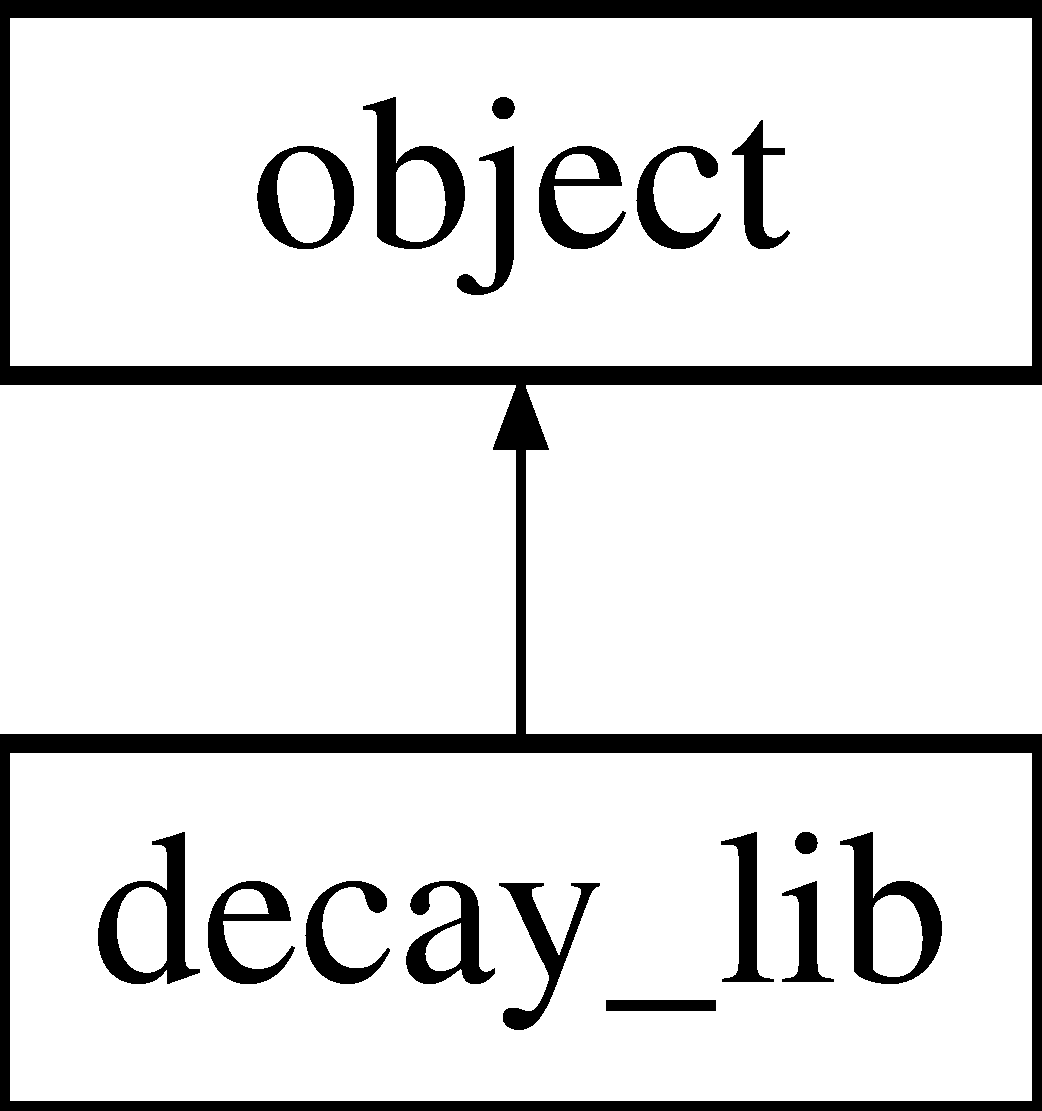
\includegraphics[height=2.000000cm]{classopenbu_1_1utils_1_1reactions__class_1_1decay__lib}
\end{center}
\end{figure}
\subsection*{Public Member Functions}
\subsection*{Private Attributes}


\subsection{Constructor \& Destructor Documentation}
\mbox{\Hypertarget{classopenbu_1_1utils_1_1reactions__class_1_1decay__lib_ae4664a4675345d114311cbd0ac402a0a}\label{classopenbu_1_1utils_1_1reactions__class_1_1decay__lib_ae4664a4675345d114311cbd0ac402a0a}} 
\index{openbu\+::utils\+::reactions\+\_\+class\+::decay\+\_\+lib@{openbu\+::utils\+::reactions\+\_\+class\+::decay\+\_\+lib}!\+\_\+\+\_\+init\+\_\+\+\_\+@{\+\_\+\+\_\+init\+\_\+\+\_\+}}
\index{\+\_\+\+\_\+init\+\_\+\+\_\+@{\+\_\+\+\_\+init\+\_\+\+\_\+}!openbu\+::utils\+::reactions\+\_\+class\+::decay\+\_\+lib@{openbu\+::utils\+::reactions\+\_\+class\+::decay\+\_\+lib}}
\subsubsection{\texorpdfstring{\+\_\+\+\_\+init\+\_\+\+\_\+()}{\_\_init\_\_()}}
{\footnotesize\ttfamily def \+\_\+\+\_\+init\+\_\+\+\_\+ (\begin{DoxyParamCaption}\item[{}]{self,  }\item[{}]{id\+\_\+number }\end{DoxyParamCaption})}



\subsection{Member Function Documentation}
\mbox{\Hypertarget{classopenbu_1_1utils_1_1reactions__class_1_1decay__lib_a794d3e0075d1c1b67e14535e6e62549a}\label{classopenbu_1_1utils_1_1reactions__class_1_1decay__lib_a794d3e0075d1c1b67e14535e6e62549a}} 
\index{openbu\+::utils\+::reactions\+\_\+class\+::decay\+\_\+lib@{openbu\+::utils\+::reactions\+\_\+class\+::decay\+\_\+lib}!add\+\_\+data@{add\+\_\+data}}
\index{add\+\_\+data@{add\+\_\+data}!openbu\+::utils\+::reactions\+\_\+class\+::decay\+\_\+lib@{openbu\+::utils\+::reactions\+\_\+class\+::decay\+\_\+lib}}
\subsubsection{\texorpdfstring{add\+\_\+data()}{add\_data()}}
{\footnotesize\ttfamily def add\+\_\+data (\begin{DoxyParamCaption}\item[{}]{self,  }\item[{}]{zamid,  }\item[{}]{kwargs }\end{DoxyParamCaption})}

\mbox{\Hypertarget{classopenbu_1_1utils_1_1reactions__class_1_1decay__lib_a3421376f5121500f9eb2b16677e8ed1e}\label{classopenbu_1_1utils_1_1reactions__class_1_1decay__lib_a3421376f5121500f9eb2b16677e8ed1e}} 
\index{openbu\+::utils\+::reactions\+\_\+class\+::decay\+\_\+lib@{openbu\+::utils\+::reactions\+\_\+class\+::decay\+\_\+lib}!create\+\_\+decay\+\_\+a@{create\+\_\+decay\+\_\+a}}
\index{create\+\_\+decay\+\_\+a@{create\+\_\+decay\+\_\+a}!openbu\+::utils\+::reactions\+\_\+class\+::decay\+\_\+lib@{openbu\+::utils\+::reactions\+\_\+class\+::decay\+\_\+lib}}
\subsubsection{\texorpdfstring{create\+\_\+decay\+\_\+a()}{create\_decay\_a()}}
{\footnotesize\ttfamily def create\+\_\+decay\+\_\+a (\begin{DoxyParamCaption}\item[{}]{self,  }\item[{}]{zamid,  }\item[{}]{dic }\end{DoxyParamCaption})}

\mbox{\Hypertarget{classopenbu_1_1utils_1_1reactions__class_1_1decay__lib_a0edaec2df85399cf219e36782994d43f}\label{classopenbu_1_1utils_1_1reactions__class_1_1decay__lib_a0edaec2df85399cf219e36782994d43f}} 
\index{openbu\+::utils\+::reactions\+\_\+class\+::decay\+\_\+lib@{openbu\+::utils\+::reactions\+\_\+class\+::decay\+\_\+lib}!create\+\_\+decay\+\_\+b@{create\+\_\+decay\+\_\+b}}
\index{create\+\_\+decay\+\_\+b@{create\+\_\+decay\+\_\+b}!openbu\+::utils\+::reactions\+\_\+class\+::decay\+\_\+lib@{openbu\+::utils\+::reactions\+\_\+class\+::decay\+\_\+lib}}
\subsubsection{\texorpdfstring{create\+\_\+decay\+\_\+b()}{create\_decay\_b()}}
{\footnotesize\ttfamily def create\+\_\+decay\+\_\+b (\begin{DoxyParamCaption}\item[{}]{self,  }\item[{}]{zamid,  }\item[{}]{dic }\end{DoxyParamCaption})}

\mbox{\Hypertarget{classopenbu_1_1utils_1_1reactions__class_1_1decay__lib_ab9d903431dc1a815d57cb09912e41e58}\label{classopenbu_1_1utils_1_1reactions__class_1_1decay__lib_ab9d903431dc1a815d57cb09912e41e58}} 
\index{openbu\+::utils\+::reactions\+\_\+class\+::decay\+\_\+lib@{openbu\+::utils\+::reactions\+\_\+class\+::decay\+\_\+lib}!decay\+\_\+a@{decay\+\_\+a}}
\index{decay\+\_\+a@{decay\+\_\+a}!openbu\+::utils\+::reactions\+\_\+class\+::decay\+\_\+lib@{openbu\+::utils\+::reactions\+\_\+class\+::decay\+\_\+lib}}
\subsubsection{\texorpdfstring{decay\+\_\+a()}{decay\_a()}}
{\footnotesize\ttfamily def decay\+\_\+a (\begin{DoxyParamCaption}\item[{}]{self }\end{DoxyParamCaption})}

\mbox{\Hypertarget{classopenbu_1_1utils_1_1reactions__class_1_1decay__lib_ade7165602b6bcdee1ed9b7256170379b}\label{classopenbu_1_1utils_1_1reactions__class_1_1decay__lib_ade7165602b6bcdee1ed9b7256170379b}} 
\index{openbu\+::utils\+::reactions\+\_\+class\+::decay\+\_\+lib@{openbu\+::utils\+::reactions\+\_\+class\+::decay\+\_\+lib}!decay\+\_\+b@{decay\+\_\+b}}
\index{decay\+\_\+b@{decay\+\_\+b}!openbu\+::utils\+::reactions\+\_\+class\+::decay\+\_\+lib@{openbu\+::utils\+::reactions\+\_\+class\+::decay\+\_\+lib}}
\subsubsection{\texorpdfstring{decay\+\_\+b()}{decay\_b()}}
{\footnotesize\ttfamily def decay\+\_\+b (\begin{DoxyParamCaption}\item[{}]{self }\end{DoxyParamCaption})}

\mbox{\Hypertarget{classopenbu_1_1utils_1_1reactions__class_1_1decay__lib_a80c88c99e45178594b9dc49b8852ee7e}\label{classopenbu_1_1utils_1_1reactions__class_1_1decay__lib_a80c88c99e45178594b9dc49b8852ee7e}} 
\index{openbu\+::utils\+::reactions\+\_\+class\+::decay\+\_\+lib@{openbu\+::utils\+::reactions\+\_\+class\+::decay\+\_\+lib}!dic@{dic}}
\index{dic@{dic}!openbu\+::utils\+::reactions\+\_\+class\+::decay\+\_\+lib@{openbu\+::utils\+::reactions\+\_\+class\+::decay\+\_\+lib}}
\subsubsection{\texorpdfstring{dic()}{dic()}}
{\footnotesize\ttfamily def dic (\begin{DoxyParamCaption}\item[{}]{self }\end{DoxyParamCaption})}



\subsection{Member Data Documentation}
\mbox{\Hypertarget{classopenbu_1_1utils_1_1reactions__class_1_1decay__lib_a1c2b24934d5eafbd256785b158a470a6}\label{classopenbu_1_1utils_1_1reactions__class_1_1decay__lib_a1c2b24934d5eafbd256785b158a470a6}} 
\index{openbu\+::utils\+::reactions\+\_\+class\+::decay\+\_\+lib@{openbu\+::utils\+::reactions\+\_\+class\+::decay\+\_\+lib}!\+\_\+decay\+\_\+a@{\+\_\+decay\+\_\+a}}
\index{\+\_\+decay\+\_\+a@{\+\_\+decay\+\_\+a}!openbu\+::utils\+::reactions\+\_\+class\+::decay\+\_\+lib@{openbu\+::utils\+::reactions\+\_\+class\+::decay\+\_\+lib}}
\subsubsection{\texorpdfstring{\+\_\+decay\+\_\+a}{\_decay\_a}}
{\footnotesize\ttfamily \+\_\+decay\+\_\+a\hspace{0.3cm}{\ttfamily [private]}}

\mbox{\Hypertarget{classopenbu_1_1utils_1_1reactions__class_1_1decay__lib_a74aadd383f9c57cbbfbb13289c5cc96f}\label{classopenbu_1_1utils_1_1reactions__class_1_1decay__lib_a74aadd383f9c57cbbfbb13289c5cc96f}} 
\index{openbu\+::utils\+::reactions\+\_\+class\+::decay\+\_\+lib@{openbu\+::utils\+::reactions\+\_\+class\+::decay\+\_\+lib}!\+\_\+decay\+\_\+b@{\+\_\+decay\+\_\+b}}
\index{\+\_\+decay\+\_\+b@{\+\_\+decay\+\_\+b}!openbu\+::utils\+::reactions\+\_\+class\+::decay\+\_\+lib@{openbu\+::utils\+::reactions\+\_\+class\+::decay\+\_\+lib}}
\subsubsection{\texorpdfstring{\+\_\+decay\+\_\+b}{\_decay\_b}}
{\footnotesize\ttfamily \+\_\+decay\+\_\+b\hspace{0.3cm}{\ttfamily [private]}}

\mbox{\Hypertarget{classopenbu_1_1utils_1_1reactions__class_1_1decay__lib_a67eb8fb1879c0d58ee16d390cfd736e4}\label{classopenbu_1_1utils_1_1reactions__class_1_1decay__lib_a67eb8fb1879c0d58ee16d390cfd736e4}} 
\index{openbu\+::utils\+::reactions\+\_\+class\+::decay\+\_\+lib@{openbu\+::utils\+::reactions\+\_\+class\+::decay\+\_\+lib}!\+\_\+dic@{\+\_\+dic}}
\index{\+\_\+dic@{\+\_\+dic}!openbu\+::utils\+::reactions\+\_\+class\+::decay\+\_\+lib@{openbu\+::utils\+::reactions\+\_\+class\+::decay\+\_\+lib}}
\subsubsection{\texorpdfstring{\+\_\+dic}{\_dic}}
{\footnotesize\ttfamily \+\_\+dic\hspace{0.3cm}{\ttfamily [private]}}

\mbox{\Hypertarget{classopenbu_1_1utils_1_1reactions__class_1_1decay__lib_aa1313b5b76f38d461c99c9a42b437f74}\label{classopenbu_1_1utils_1_1reactions__class_1_1decay__lib_aa1313b5b76f38d461c99c9a42b437f74}} 
\index{openbu\+::utils\+::reactions\+\_\+class\+::decay\+\_\+lib@{openbu\+::utils\+::reactions\+\_\+class\+::decay\+\_\+lib}!\+\_\+id@{\+\_\+id}}
\index{\+\_\+id@{\+\_\+id}!openbu\+::utils\+::reactions\+\_\+class\+::decay\+\_\+lib@{openbu\+::utils\+::reactions\+\_\+class\+::decay\+\_\+lib}}
\subsubsection{\texorpdfstring{\+\_\+id}{\_id}}
{\footnotesize\ttfamily \+\_\+id\hspace{0.3cm}{\ttfamily [private]}}



The documentation for this class was generated from the following file\+:\begin{DoxyCompactItemize}
\item 
/\+Users/mouginot/work/app/\+Open\+B\+U/openbu/utils/\mbox{\hyperlink{reactions__class_8py}{reactions\+\_\+class.\+py}}\end{DoxyCompactItemize}

\hypertarget{classopenbu_1_1utils_1_1functions_1_1_empty__argument}{}\doxysection{Empty\+\_\+argument Class Reference}
\label{classopenbu_1_1utils_1_1functions_1_1_empty__argument}\index{Empty\_argument@{Empty\_argument}}
Inheritance diagram for Empty\+\_\+argument\+:\begin{figure}[H]
\begin{center}
\leavevmode
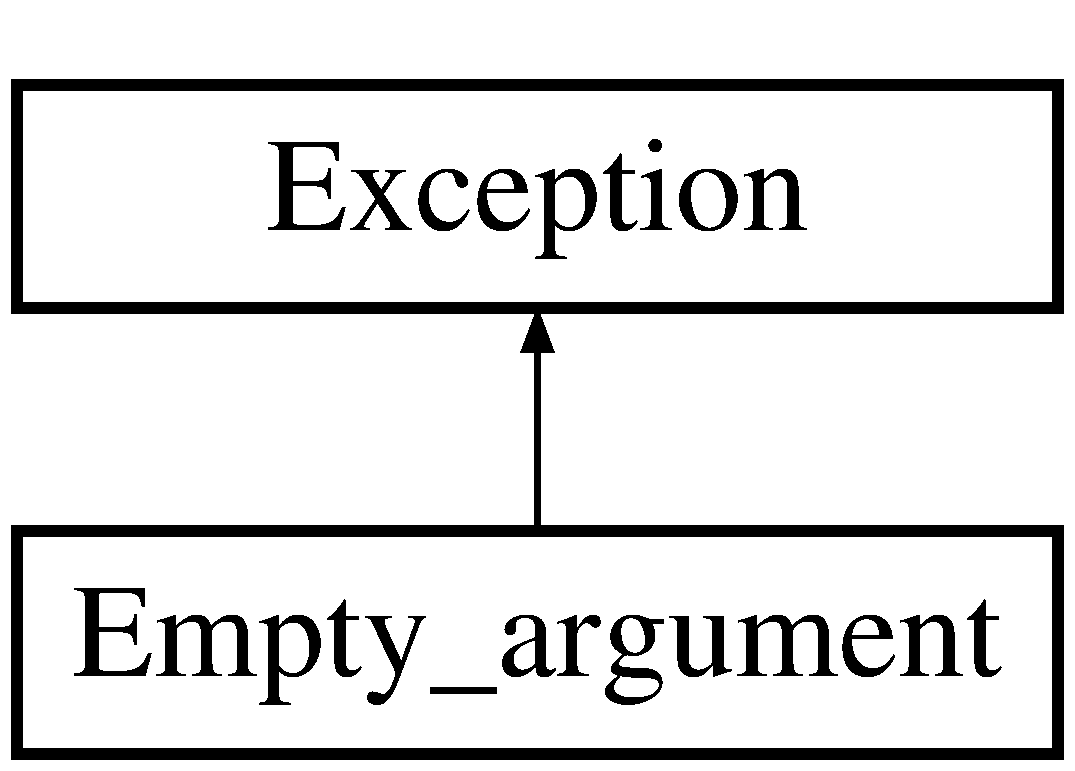
\includegraphics[height=2.000000cm]{classopenbu_1_1utils_1_1functions_1_1_empty__argument}
\end{center}
\end{figure}


\doxysubsection{Detailed Description}
\begin{DoxyVerb}Raise when the user calls decay_halflife_conv without entering any argument \end{DoxyVerb}
 

The documentation for this class was generated from the following file\+:\begin{DoxyCompactItemize}
\item 
utils/functions.\+py\end{DoxyCompactItemize}

\hypertarget{classopenbu_1_1utils_1_1reactions__class_1_1_empty__data}{}\section{Empty\+\_\+data Class Reference}
\label{classopenbu_1_1utils_1_1reactions__class_1_1_empty__data}\index{Empty\+\_\+data@{Empty\+\_\+data}}
Inheritance diagram for Empty\+\_\+data\+:\begin{figure}[H]
\begin{center}
\leavevmode
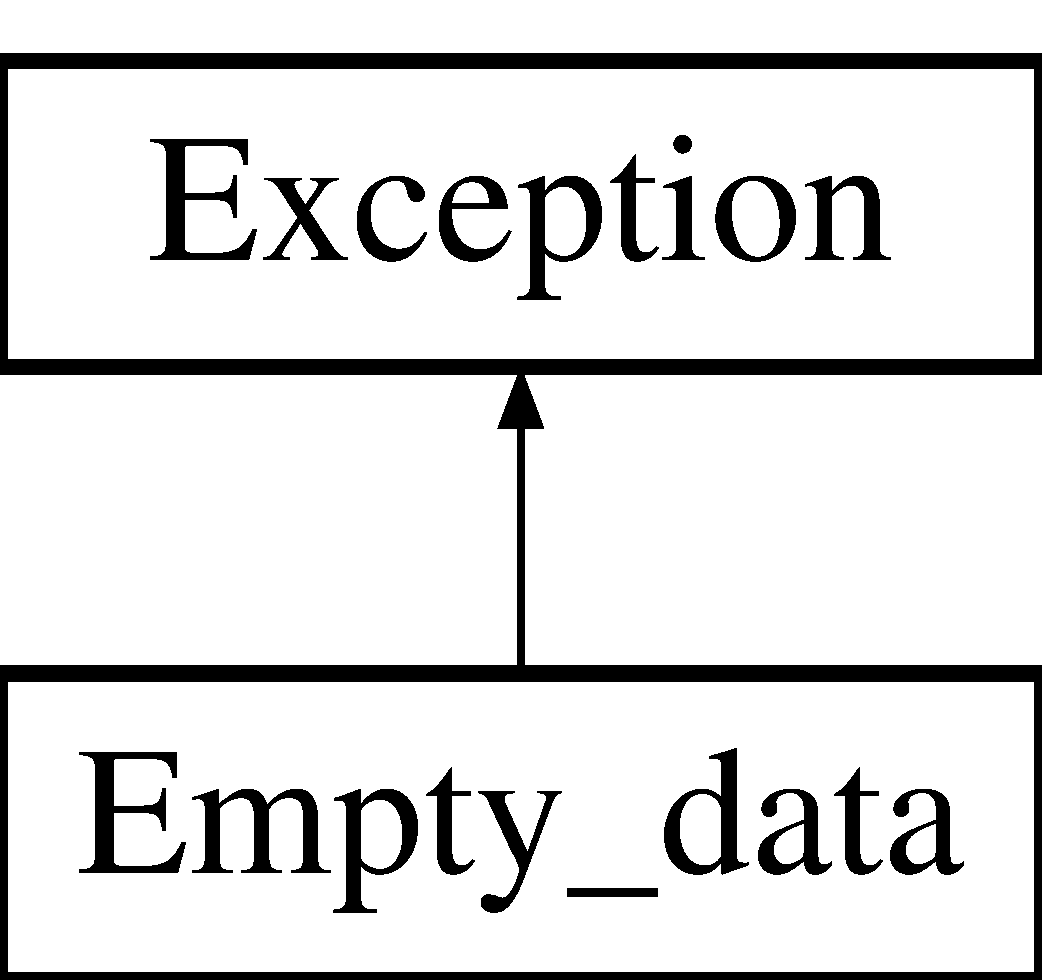
\includegraphics[height=2.000000cm]{classopenbu_1_1utils_1_1reactions__class_1_1_empty__data}
\end{center}
\end{figure}


\subsection{Detailed Description}
\begin{DoxyVerb}Raise when the user does not enter any data while add_data has been called for a nuclide\end{DoxyVerb}
 

The documentation for this class was generated from the following file\+:\begin{DoxyCompactItemize}
\item 
/\+Users/mouginot/work/app/\+Open\+B\+U/openbu/utils/reactions\+\_\+class.\+py\end{DoxyCompactItemize}

\hypertarget{classopenbu_1_1utils_1_1reactions__class_1_1fy__lib}{}\section{fy\+\_\+lib Class Reference}
\label{classopenbu_1_1utils_1_1reactions__class_1_1fy__lib}\index{fy\+\_\+lib@{fy\+\_\+lib}}
Inheritance diagram for fy\+\_\+lib\+:\begin{figure}[H]
\begin{center}
\leavevmode
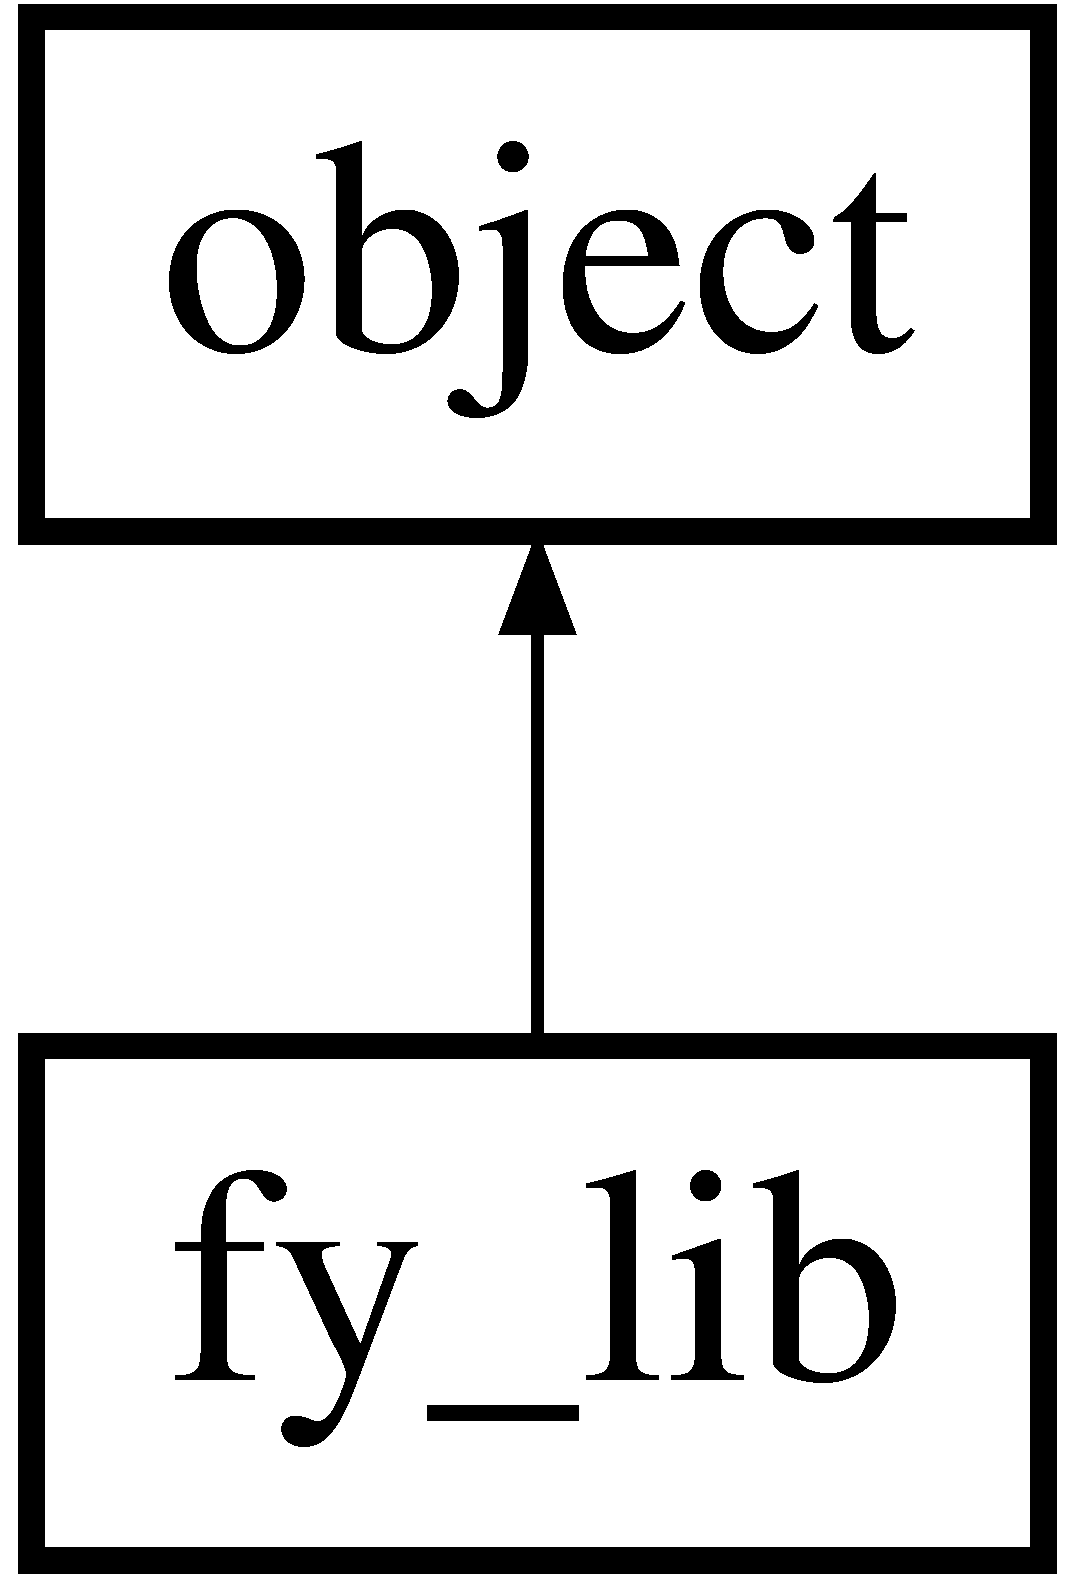
\includegraphics[height=2.000000cm]{classopenbu_1_1utils_1_1reactions__class_1_1fy__lib}
\end{center}
\end{figure}
\subsection*{Public Member Functions}
\subsection*{Private Attributes}


\subsection{Constructor \& Destructor Documentation}
\mbox{\Hypertarget{classopenbu_1_1utils_1_1reactions__class_1_1fy__lib_ae4664a4675345d114311cbd0ac402a0a}\label{classopenbu_1_1utils_1_1reactions__class_1_1fy__lib_ae4664a4675345d114311cbd0ac402a0a}} 
\index{openbu\+::utils\+::reactions\+\_\+class\+::fy\+\_\+lib@{openbu\+::utils\+::reactions\+\_\+class\+::fy\+\_\+lib}!\+\_\+\+\_\+init\+\_\+\+\_\+@{\+\_\+\+\_\+init\+\_\+\+\_\+}}
\index{\+\_\+\+\_\+init\+\_\+\+\_\+@{\+\_\+\+\_\+init\+\_\+\+\_\+}!openbu\+::utils\+::reactions\+\_\+class\+::fy\+\_\+lib@{openbu\+::utils\+::reactions\+\_\+class\+::fy\+\_\+lib}}
\subsubsection{\texorpdfstring{\+\_\+\+\_\+init\+\_\+\+\_\+()}{\_\_init\_\_()}}
{\footnotesize\ttfamily def \+\_\+\+\_\+init\+\_\+\+\_\+ (\begin{DoxyParamCaption}\item[{}]{self,  }\item[{}]{id\+\_\+number }\end{DoxyParamCaption})}



\subsection{Member Function Documentation}
\mbox{\Hypertarget{classopenbu_1_1utils_1_1reactions__class_1_1fy__lib_ab51433137df38fc8bd763ceda7026af2}\label{classopenbu_1_1utils_1_1reactions__class_1_1fy__lib_ab51433137df38fc8bd763ceda7026af2}} 
\index{openbu\+::utils\+::reactions\+\_\+class\+::fy\+\_\+lib@{openbu\+::utils\+::reactions\+\_\+class\+::fy\+\_\+lib}!add\+\_\+data@{add\+\_\+data}}
\index{add\+\_\+data@{add\+\_\+data}!openbu\+::utils\+::reactions\+\_\+class\+::fy\+\_\+lib@{openbu\+::utils\+::reactions\+\_\+class\+::fy\+\_\+lib}}
\subsubsection{\texorpdfstring{add\+\_\+data()}{add\_data()}}
{\footnotesize\ttfamily def add\+\_\+data (\begin{DoxyParamCaption}\item[{}]{self,  }\item[{}]{zamid,  }\item[{}]{dic }\end{DoxyParamCaption})}

\mbox{\Hypertarget{classopenbu_1_1utils_1_1reactions__class_1_1fy__lib_a8b75ace3008810461600cc7df511303b}\label{classopenbu_1_1utils_1_1reactions__class_1_1fy__lib_a8b75ace3008810461600cc7df511303b}} 
\index{openbu\+::utils\+::reactions\+\_\+class\+::fy\+\_\+lib@{openbu\+::utils\+::reactions\+\_\+class\+::fy\+\_\+lib}!fy@{fy}}
\index{fy@{fy}!openbu\+::utils\+::reactions\+\_\+class\+::fy\+\_\+lib@{openbu\+::utils\+::reactions\+\_\+class\+::fy\+\_\+lib}}
\subsubsection{\texorpdfstring{fy()}{fy()}}
{\footnotesize\ttfamily def fy (\begin{DoxyParamCaption}\item[{}]{self }\end{DoxyParamCaption})}



\subsection{Member Data Documentation}
\mbox{\Hypertarget{classopenbu_1_1utils_1_1reactions__class_1_1fy__lib_a67eb8fb1879c0d58ee16d390cfd736e4}\label{classopenbu_1_1utils_1_1reactions__class_1_1fy__lib_a67eb8fb1879c0d58ee16d390cfd736e4}} 
\index{openbu\+::utils\+::reactions\+\_\+class\+::fy\+\_\+lib@{openbu\+::utils\+::reactions\+\_\+class\+::fy\+\_\+lib}!\+\_\+dic@{\+\_\+dic}}
\index{\+\_\+dic@{\+\_\+dic}!openbu\+::utils\+::reactions\+\_\+class\+::fy\+\_\+lib@{openbu\+::utils\+::reactions\+\_\+class\+::fy\+\_\+lib}}
\subsubsection{\texorpdfstring{\+\_\+dic}{\_dic}}
{\footnotesize\ttfamily \+\_\+dic\hspace{0.3cm}{\ttfamily [private]}}

\mbox{\Hypertarget{classopenbu_1_1utils_1_1reactions__class_1_1fy__lib_a47fe437d4dacfd52d3296390e1bd67f8}\label{classopenbu_1_1utils_1_1reactions__class_1_1fy__lib_a47fe437d4dacfd52d3296390e1bd67f8}} 
\index{openbu\+::utils\+::reactions\+\_\+class\+::fy\+\_\+lib@{openbu\+::utils\+::reactions\+\_\+class\+::fy\+\_\+lib}!\+\_\+fy@{\+\_\+fy}}
\index{\+\_\+fy@{\+\_\+fy}!openbu\+::utils\+::reactions\+\_\+class\+::fy\+\_\+lib@{openbu\+::utils\+::reactions\+\_\+class\+::fy\+\_\+lib}}
\subsubsection{\texorpdfstring{\+\_\+fy}{\_fy}}
{\footnotesize\ttfamily \+\_\+fy\hspace{0.3cm}{\ttfamily [private]}}

\mbox{\Hypertarget{classopenbu_1_1utils_1_1reactions__class_1_1fy__lib_aa1313b5b76f38d461c99c9a42b437f74}\label{classopenbu_1_1utils_1_1reactions__class_1_1fy__lib_aa1313b5b76f38d461c99c9a42b437f74}} 
\index{openbu\+::utils\+::reactions\+\_\+class\+::fy\+\_\+lib@{openbu\+::utils\+::reactions\+\_\+class\+::fy\+\_\+lib}!\+\_\+id@{\+\_\+id}}
\index{\+\_\+id@{\+\_\+id}!openbu\+::utils\+::reactions\+\_\+class\+::fy\+\_\+lib@{openbu\+::utils\+::reactions\+\_\+class\+::fy\+\_\+lib}}
\subsubsection{\texorpdfstring{\+\_\+id}{\_id}}
{\footnotesize\ttfamily \+\_\+id\hspace{0.3cm}{\ttfamily [private]}}



The documentation for this class was generated from the following file\+:\begin{DoxyCompactItemize}
\item 
/\+Users/mouginot/work/app/\+Open\+B\+U/openbu/utils/\mbox{\hyperlink{reactions__class_8py}{reactions\+\_\+class.\+py}}\end{DoxyCompactItemize}

\hypertarget{classopenbu_1_1passport_1_1_incorrect__nuc__id}{}\section{Incorrect\+\_\+nuc\+\_\+id Class Reference}
\label{classopenbu_1_1passport_1_1_incorrect__nuc__id}\index{Incorrect\+\_\+nuc\+\_\+id@{Incorrect\+\_\+nuc\+\_\+id}}
Inheritance diagram for Incorrect\+\_\+nuc\+\_\+id\+:\begin{figure}[H]
\begin{center}
\leavevmode
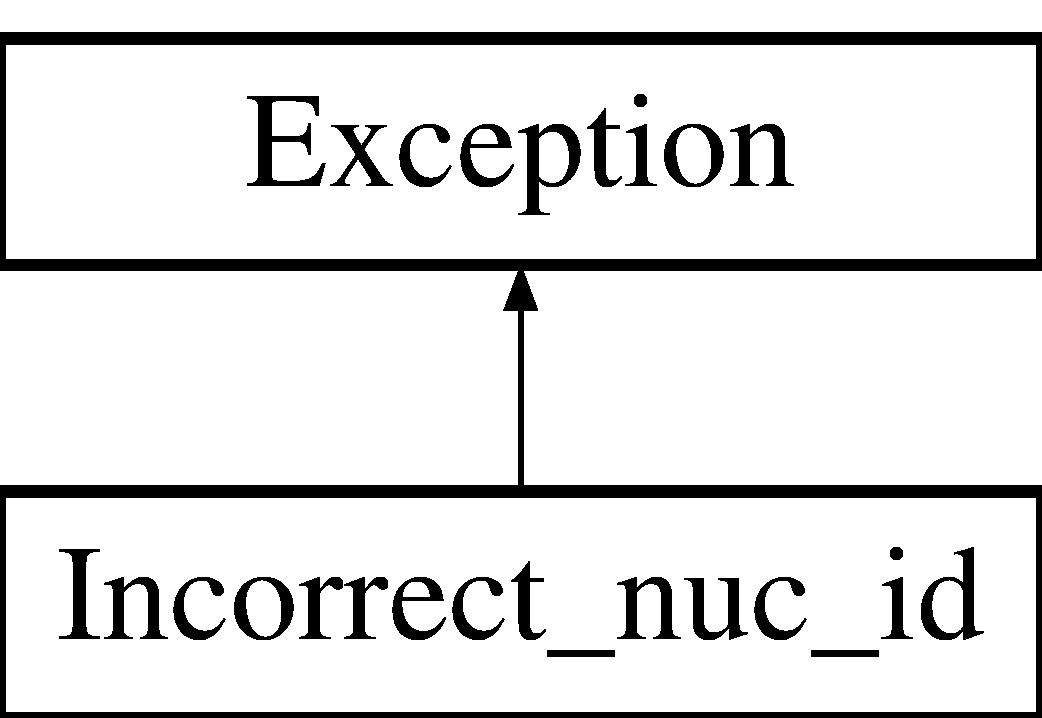
\includegraphics[height=2.000000cm]{classopenbu_1_1passport_1_1_incorrect__nuc__id}
\end{center}
\end{figure}


\subsection{Detailed Description}
\begin{DoxyVerb}Raise when the id input format in passport instantiation is incorrect\end{DoxyVerb}
 

The documentation for this class was generated from the following file\+:\begin{DoxyCompactItemize}
\item 
/\+Users/mouginot/work/app/\+Open\+B\+U/openbu/\mbox{\hyperlink{passport_8py}{passport.\+py}}\end{DoxyCompactItemize}

\hypertarget{classopenbu_1_1cell_1_1_initial__nucl__not__in___nucl__set}{}\section{Initial\+\_\+nucl\+\_\+not\+\_\+in\+\_\+\+Nucl\+\_\+set Class Reference}
\label{classopenbu_1_1cell_1_1_initial__nucl__not__in___nucl__set}\index{Initial\+\_\+nucl\+\_\+not\+\_\+in\+\_\+\+Nucl\+\_\+set@{Initial\+\_\+nucl\+\_\+not\+\_\+in\+\_\+\+Nucl\+\_\+set}}
Inheritance diagram for Initial\+\_\+nucl\+\_\+not\+\_\+in\+\_\+\+Nucl\+\_\+set\+:\begin{figure}[H]
\begin{center}
\leavevmode
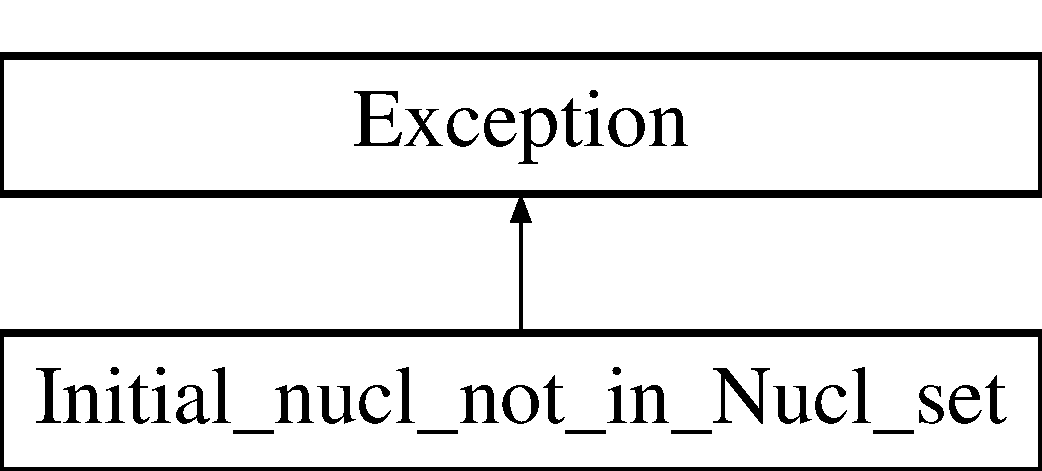
\includegraphics[height=2.000000cm]{classopenbu_1_1cell_1_1_initial__nucl__not__in___nucl__set}
\end{center}
\end{figure}


\subsection{Detailed Description}
\begin{DoxyVerb}Raise when the user forgot to set the initial nuclide of the cell and tries to burn cell\end{DoxyVerb}
 

The documentation for this class was generated from the following file\+:\begin{DoxyCompactItemize}
\item 
/\+Users/mouginot/work/app/\+Open\+B\+U/openbu/\mbox{\hyperlink{cell_8py}{cell.\+py}}\end{DoxyCompactItemize}

\hypertarget{classopenbu_1_1cell_1_1_initial__nucl__not__set}{}\doxysection{Initial\+\_\+nucl\+\_\+not\+\_\+set Class Reference}
\label{classopenbu_1_1cell_1_1_initial__nucl__not__set}\index{Initial\_nucl\_not\_set@{Initial\_nucl\_not\_set}}
Inheritance diagram for Initial\+\_\+nucl\+\_\+not\+\_\+set\+:\begin{figure}[H]
\begin{center}
\leavevmode
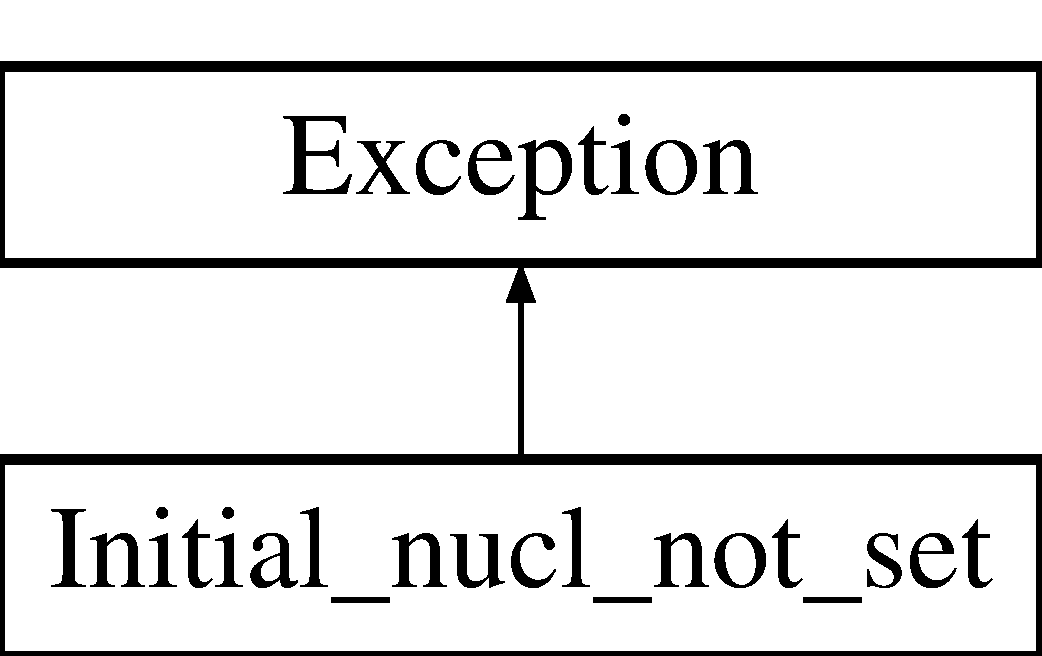
\includegraphics[height=2.000000cm]{classopenbu_1_1cell_1_1_initial__nucl__not__set}
\end{center}
\end{figure}


\doxysubsection{Detailed Description}
\begin{DoxyVerb}Raise when the user forgot to set the initial nuclide of the cell and tries to burn cell\end{DoxyVerb}
 

The documentation for this class was generated from the following file\+:\begin{DoxyCompactItemize}
\item 
cell.\+py\end{DoxyCompactItemize}

\hypertarget{classopenbu_1_1couple_1_1couple__openmc_1_1_initial__nuclides__not__in__nuclide__list}{}\section{Initial\+\_\+nuclides\+\_\+not\+\_\+in\+\_\+nuclide\+\_\+list Class Reference}
\label{classopenbu_1_1couple_1_1couple__openmc_1_1_initial__nuclides__not__in__nuclide__list}\index{Initial\+\_\+nuclides\+\_\+not\+\_\+in\+\_\+nuclide\+\_\+list@{Initial\+\_\+nuclides\+\_\+not\+\_\+in\+\_\+nuclide\+\_\+list}}
Inheritance diagram for Initial\+\_\+nuclides\+\_\+not\+\_\+in\+\_\+nuclide\+\_\+list\+:\begin{figure}[H]
\begin{center}
\leavevmode
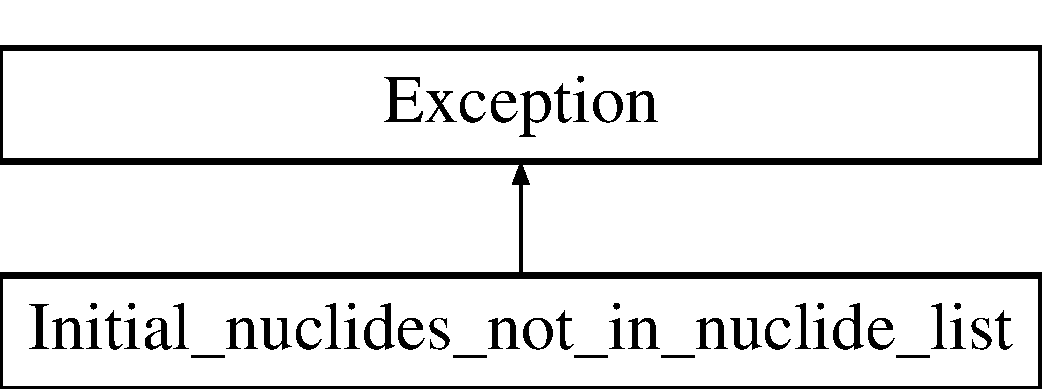
\includegraphics[height=2.000000cm]{classopenbu_1_1couple_1_1couple__openmc_1_1_initial__nuclides__not__in__nuclide__list}
\end{center}
\end{figure}


\subsection{Detailed Description}
\begin{DoxyVerb}Raise when some initial nuclides are not included in nucl_list \end{DoxyVerb}
 

The documentation for this class was generated from the following file\+:\begin{DoxyCompactItemize}
\item 
/\+Users/mouginot/work/app/\+Open\+B\+U/openbu/couple/\mbox{\hyperlink{couple__openmc_8py}{couple\+\_\+openmc.\+py}}\end{DoxyCompactItemize}

\hypertarget{classopenbu_1_1input_1_1_input}{}\doxysection{Input Class Reference}
\label{classopenbu_1_1input_1_1_input}\index{Input@{Input}}
Inheritance diagram for Input\+:\begin{figure}[H]
\begin{center}
\leavevmode
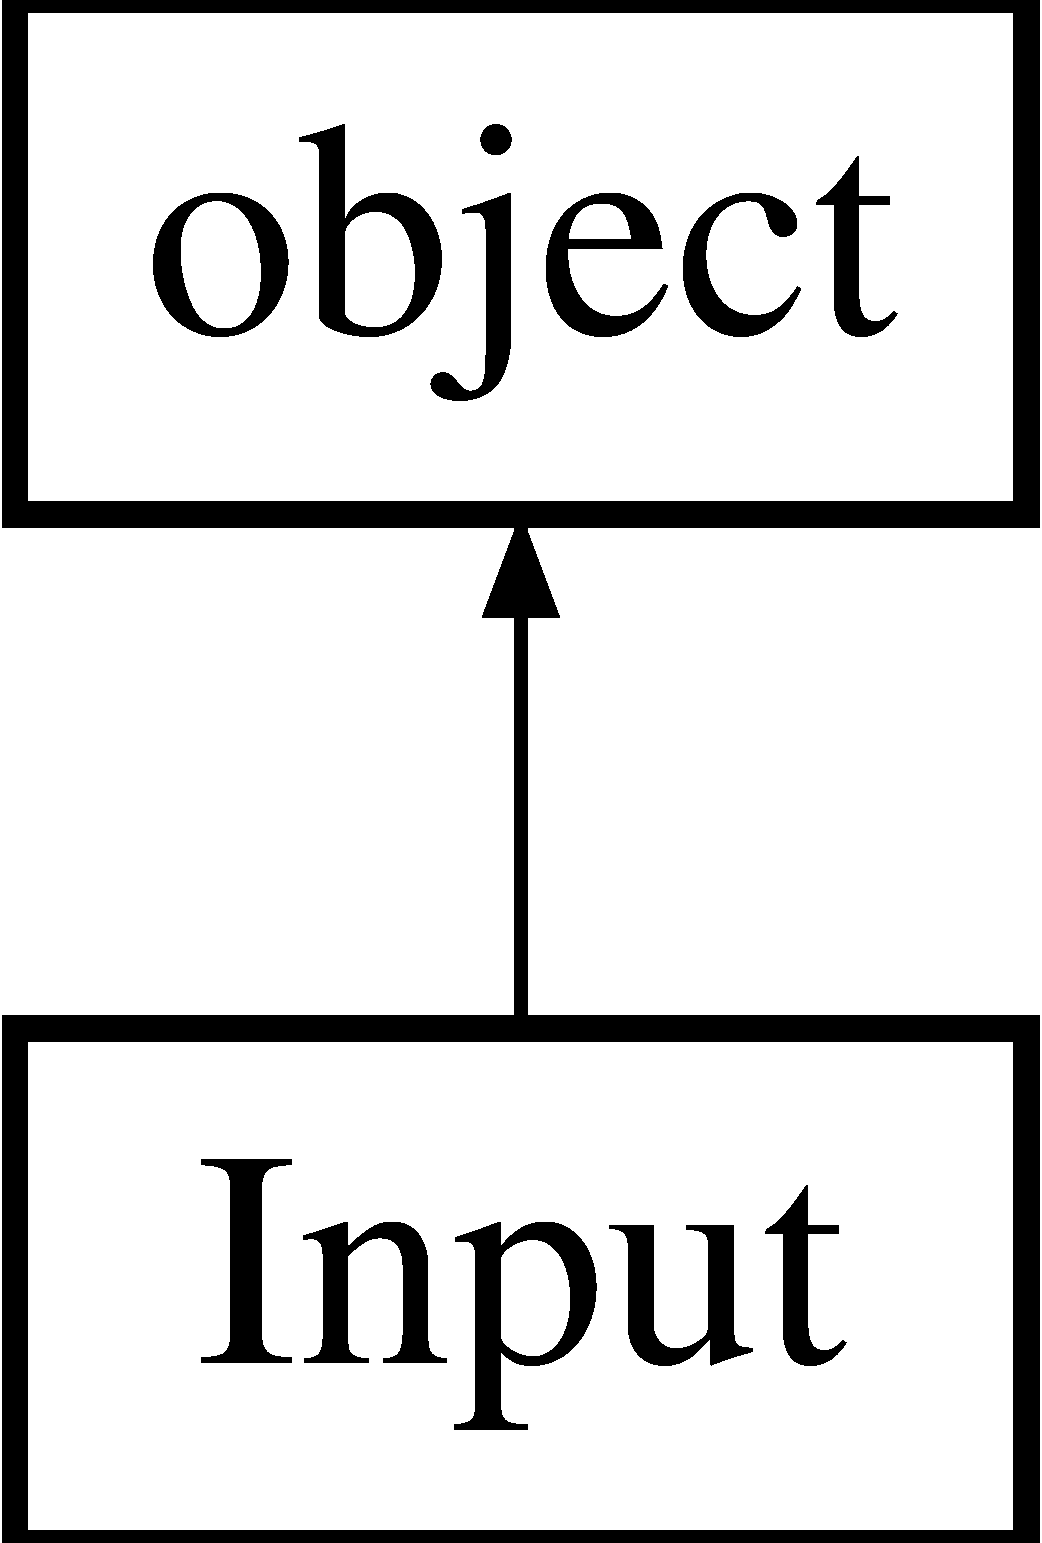
\includegraphics[height=2.000000cm]{classopenbu_1_1input_1_1_input}
\end{center}
\end{figure}
\doxysubsection*{Public Member Functions}
\doxysubsection*{Public Attributes}
\doxysubsection*{Private Member Functions}
\doxysubsection*{Private Attributes}
\doxysubsection*{Static Private Attributes}


\doxysubsection{Detailed Description}
\begin{DoxyVerb}input reads, stores and process the input data in the input file provided by the user\end{DoxyVerb}
 

\doxysubsection{Member Function Documentation}
\mbox{\Hypertarget{classopenbu_1_1input_1_1_input_aec654cc5b1c47a58ce5dd1de926b8c17}\label{classopenbu_1_1input_1_1_input_aec654cc5b1c47a58ce5dd1de926b8c17}} 
\index{Input@{Input}!cell\_id\_list@{cell\_id\_list}}
\index{cell\_id\_list@{cell\_id\_list}!Input@{Input}}
\doxysubsubsection{\texorpdfstring{cell\_id\_list()}{cell\_id\_list()}}
{\footnotesize\ttfamily def cell\+\_\+id\+\_\+list (\begin{DoxyParamCaption}\item[{}]{self }\end{DoxyParamCaption})}

\begin{DoxyVerb}Returns the absolute values of the decay constant of the nuclide\end{DoxyVerb}
 \mbox{\Hypertarget{classopenbu_1_1input_1_1_input_ada83a03c99c1587bee0ffb75e04f0589}\label{classopenbu_1_1input_1_1_input_ada83a03c99c1587bee0ffb75e04f0589}} 
\index{Input@{Input}!cells@{cells}}
\index{cells@{cells}!Input@{Input}}
\doxysubsubsection{\texorpdfstring{cells()}{cells()}}
{\footnotesize\ttfamily def cells (\begin{DoxyParamCaption}\item[{}]{self }\end{DoxyParamCaption})}

\begin{DoxyVerb}Returns the absolute values of the decay constant of the nuclide\end{DoxyVerb}
 \mbox{\Hypertarget{classopenbu_1_1input_1_1_input_a7c74249450d6c2107885b03f5328ca75}\label{classopenbu_1_1input_1_1_input_a7c74249450d6c2107885b03f5328ca75}} 
\index{Input@{Input}!lib@{lib}}
\index{lib@{lib}!Input@{Input}}
\doxysubsubsection{\texorpdfstring{lib()}{lib()}}
{\footnotesize\ttfamily def lib (\begin{DoxyParamCaption}\item[{}]{self }\end{DoxyParamCaption})}

\begin{DoxyVerb}Returns the absolute values of the decay constant of the nuclide\end{DoxyVerb}
 \mbox{\Hypertarget{classopenbu_1_1input_1_1_input_a6ef2947c0b15938b4f351065ee10dcc9}\label{classopenbu_1_1input_1_1_input_a6ef2947c0b15938b4f351065ee10dcc9}} 
\index{Input@{Input}!mode@{mode}}
\index{mode@{mode}!Input@{Input}}
\doxysubsubsection{\texorpdfstring{mode()}{mode()}}
{\footnotesize\ttfamily def mode (\begin{DoxyParamCaption}\item[{}]{self }\end{DoxyParamCaption})}

\begin{DoxyVerb}Returns the absolute values of the decay constant of the nuclide\end{DoxyVerb}
 

The documentation for this class was generated from the following file\+:\begin{DoxyCompactItemize}
\item 
input.\+py\end{DoxyCompactItemize}

\hypertarget{classopenbu_1_1utils_1_1functions_1_1_midpoint_normalize}{}\section{Midpoint\+Normalize Class Reference}
\label{classopenbu_1_1utils_1_1functions_1_1_midpoint_normalize}\index{Midpoint\+Normalize@{Midpoint\+Normalize}}
Inheritance diagram for Midpoint\+Normalize\+:\begin{figure}[H]
\begin{center}
\leavevmode
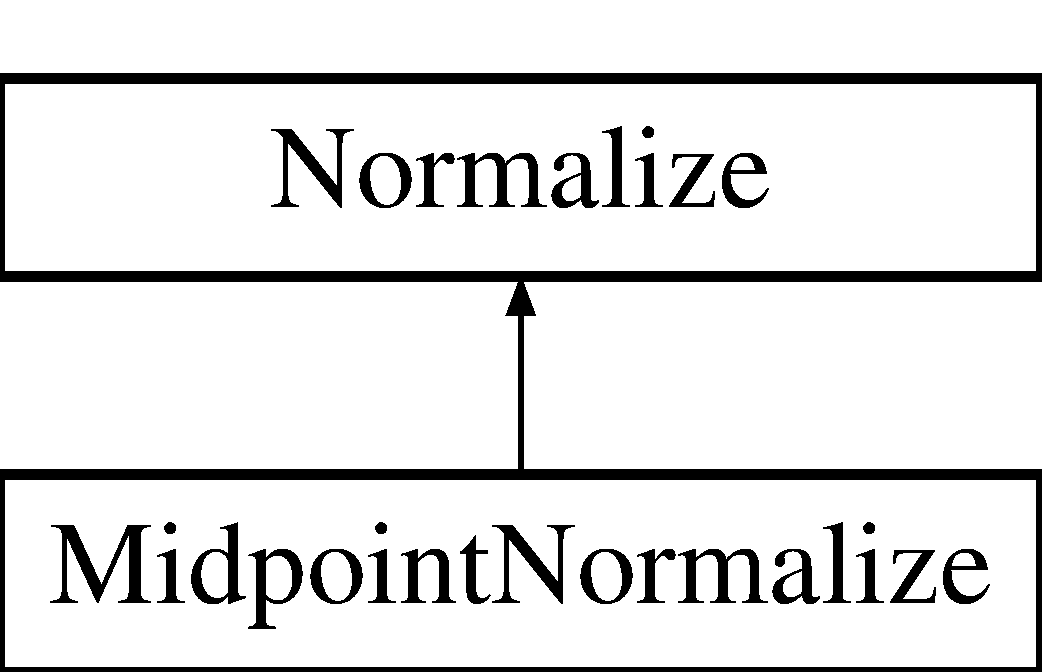
\includegraphics[height=2.000000cm]{classopenbu_1_1utils_1_1functions_1_1_midpoint_normalize}
\end{center}
\end{figure}
\subsection*{Public Member Functions}
\subsection*{Public Attributes}


\subsection{Detailed Description}
\begin{DoxyVerb}Normalise the colorbar so that diverging bars work there way either side from a prescribed midpoint value)

e.g. im=ax1.imshow(array, norm=MidpointNormalize(midpoint=0.,vmin=-100, vmax=100))
\end{DoxyVerb}
 

\subsection{Constructor \& Destructor Documentation}
\mbox{\Hypertarget{classopenbu_1_1utils_1_1functions_1_1_midpoint_normalize_a87831fcbb459c9db73a8c7ce1d07a760}\label{classopenbu_1_1utils_1_1functions_1_1_midpoint_normalize_a87831fcbb459c9db73a8c7ce1d07a760}} 
\index{openbu\+::utils\+::functions\+::\+Midpoint\+Normalize@{openbu\+::utils\+::functions\+::\+Midpoint\+Normalize}!\+\_\+\+\_\+init\+\_\+\+\_\+@{\+\_\+\+\_\+init\+\_\+\+\_\+}}
\index{\+\_\+\+\_\+init\+\_\+\+\_\+@{\+\_\+\+\_\+init\+\_\+\+\_\+}!openbu\+::utils\+::functions\+::\+Midpoint\+Normalize@{openbu\+::utils\+::functions\+::\+Midpoint\+Normalize}}
\subsubsection{\texorpdfstring{\+\_\+\+\_\+init\+\_\+\+\_\+()}{\_\_init\_\_()}}
{\footnotesize\ttfamily def \+\_\+\+\_\+init\+\_\+\+\_\+ (\begin{DoxyParamCaption}\item[{}]{self,  }\item[{}]{vmin = {\ttfamily None},  }\item[{}]{vmax = {\ttfamily None},  }\item[{}]{midpoint = {\ttfamily None},  }\item[{}]{clip = {\ttfamily False} }\end{DoxyParamCaption})}



\subsection{Member Function Documentation}
\mbox{\Hypertarget{classopenbu_1_1utils_1_1functions_1_1_midpoint_normalize_aa6cce7eb63fb71fe8f5f1bc150371618}\label{classopenbu_1_1utils_1_1functions_1_1_midpoint_normalize_aa6cce7eb63fb71fe8f5f1bc150371618}} 
\index{openbu\+::utils\+::functions\+::\+Midpoint\+Normalize@{openbu\+::utils\+::functions\+::\+Midpoint\+Normalize}!\+\_\+\+\_\+call\+\_\+\+\_\+@{\+\_\+\+\_\+call\+\_\+\+\_\+}}
\index{\+\_\+\+\_\+call\+\_\+\+\_\+@{\+\_\+\+\_\+call\+\_\+\+\_\+}!openbu\+::utils\+::functions\+::\+Midpoint\+Normalize@{openbu\+::utils\+::functions\+::\+Midpoint\+Normalize}}
\subsubsection{\texorpdfstring{\+\_\+\+\_\+call\+\_\+\+\_\+()}{\_\_call\_\_()}}
{\footnotesize\ttfamily def \+\_\+\+\_\+call\+\_\+\+\_\+ (\begin{DoxyParamCaption}\item[{}]{self,  }\item[{}]{value,  }\item[{}]{clip = {\ttfamily None} }\end{DoxyParamCaption})}



\subsection{Member Data Documentation}
\mbox{\Hypertarget{classopenbu_1_1utils_1_1functions_1_1_midpoint_normalize_af53e0eb961b2050b7ae1f7994bfed8ff}\label{classopenbu_1_1utils_1_1functions_1_1_midpoint_normalize_af53e0eb961b2050b7ae1f7994bfed8ff}} 
\index{openbu\+::utils\+::functions\+::\+Midpoint\+Normalize@{openbu\+::utils\+::functions\+::\+Midpoint\+Normalize}!midpoint@{midpoint}}
\index{midpoint@{midpoint}!openbu\+::utils\+::functions\+::\+Midpoint\+Normalize@{openbu\+::utils\+::functions\+::\+Midpoint\+Normalize}}
\subsubsection{\texorpdfstring{midpoint}{midpoint}}
{\footnotesize\ttfamily midpoint}



The documentation for this class was generated from the following file\+:\begin{DoxyCompactItemize}
\item 
/\+Users/mouginot/work/app/\+Open\+B\+U/openbu/utils/\mbox{\hyperlink{utils_2functions_8py}{functions.\+py}}\end{DoxyCompactItemize}

\hypertarget{classopenbu_1_1passlist_1_1_neg__decay}{}\doxysection{Neg\+\_\+decay Class Reference}
\label{classopenbu_1_1passlist_1_1_neg__decay}\index{Neg\_decay@{Neg\_decay}}
Inheritance diagram for Neg\+\_\+decay\+:\begin{figure}[H]
\begin{center}
\leavevmode
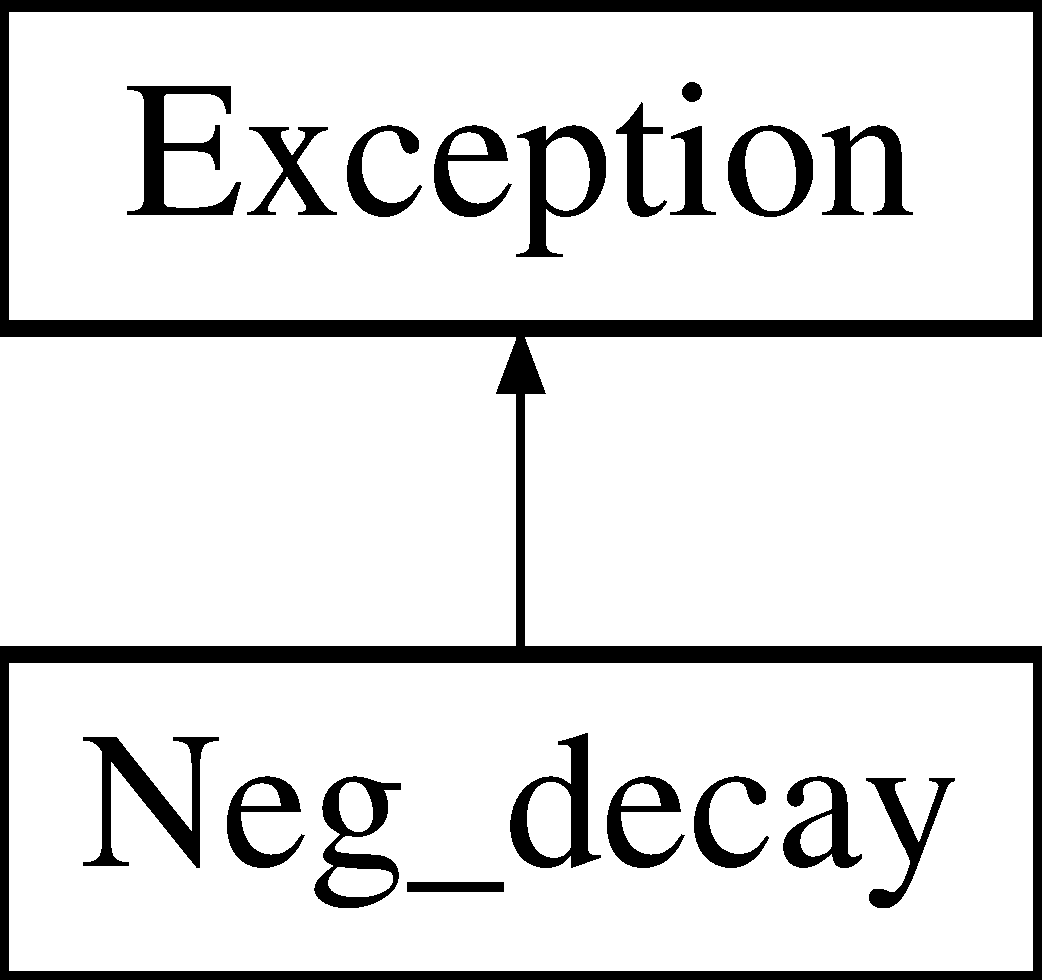
\includegraphics[height=2.000000cm]{classopenbu_1_1passlist_1_1_neg__decay}
\end{center}
\end{figure}


\doxysubsection{Detailed Description}
\begin{DoxyVerb}Raise when a negative decay constant is found\end{DoxyVerb}
 

The documentation for this class was generated from the following file\+:\begin{DoxyCompactItemize}
\item 
passlist.\+py\end{DoxyCompactItemize}

\hypertarget{classopenbu_1_1passlist_1_1_neg__xs}{}\doxysection{Neg\+\_\+xs Class Reference}
\label{classopenbu_1_1passlist_1_1_neg__xs}\index{Neg\_xs@{Neg\_xs}}
Inheritance diagram for Neg\+\_\+xs\+:\begin{figure}[H]
\begin{center}
\leavevmode
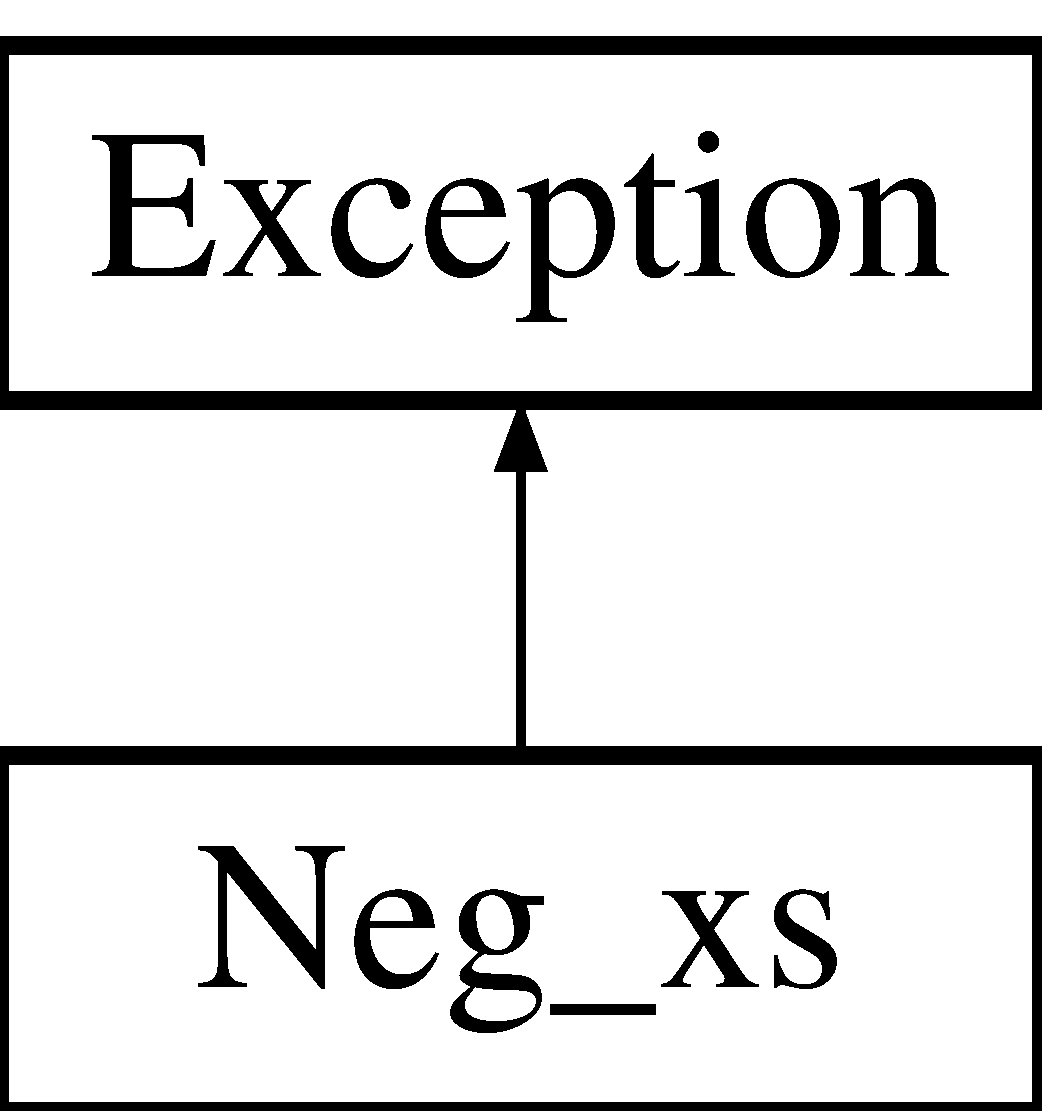
\includegraphics[height=2.000000cm]{classopenbu_1_1passlist_1_1_neg__xs}
\end{center}
\end{figure}


\doxysubsection{Detailed Description}
\begin{DoxyVerb}Raise when a negative cross-section is found\end{DoxyVerb}
 

The documentation for this class was generated from the following file\+:\begin{DoxyCompactItemize}
\item 
passlist.\+py\end{DoxyCompactItemize}

\hypertarget{classopenbu_1_1passport_1_1_no__fission___x_s}{}\section{No\+\_\+fission\+\_\+\+XS Class Reference}
\label{classopenbu_1_1passport_1_1_no__fission___x_s}\index{No\+\_\+fission\+\_\+\+XS@{No\+\_\+fission\+\_\+\+XS}}
Inheritance diagram for No\+\_\+fission\+\_\+\+XS\+:\begin{figure}[H]
\begin{center}
\leavevmode
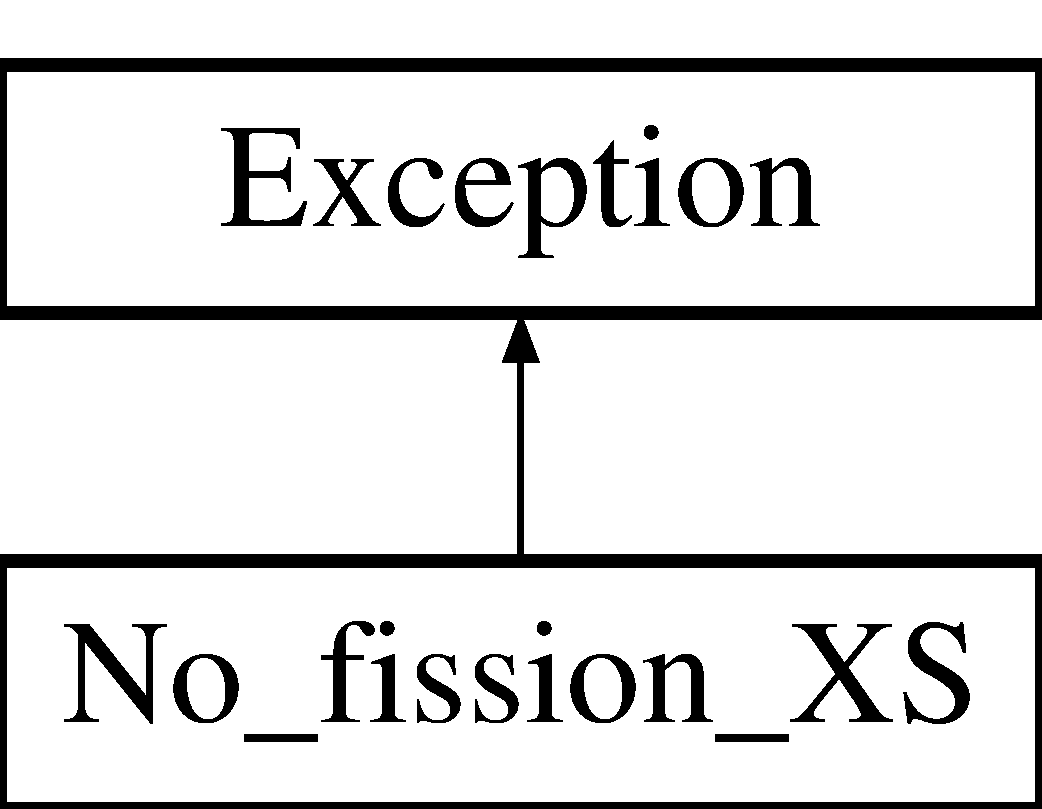
\includegraphics[height=2.000000cm]{classopenbu_1_1passport_1_1_no__fission___x_s}
\end{center}
\end{figure}


\subsection{Detailed Description}
\begin{DoxyVerb}Raise when the user tries to access fission XS for a nuclide which fission XS have not been set yet \end{DoxyVerb}
 

The documentation for this class was generated from the following file\+:\begin{DoxyCompactItemize}
\item 
/\+Users/mouginot/work/app/\+Open\+B\+U/openbu/\mbox{\hyperlink{passport_8py}{passport.\+py}}\end{DoxyCompactItemize}

\hypertarget{classopenbu_1_1passport_1_1_not__a___fission___product}{}\doxysection{Not\+\_\+a\+\_\+\+Fission\+\_\+\+Product Class Reference}
\label{classopenbu_1_1passport_1_1_not__a___fission___product}\index{Not\_a\_Fission\_Product@{Not\_a\_Fission\_Product}}
Inheritance diagram for Not\+\_\+a\+\_\+\+Fission\+\_\+\+Product\+:\begin{figure}[H]
\begin{center}
\leavevmode
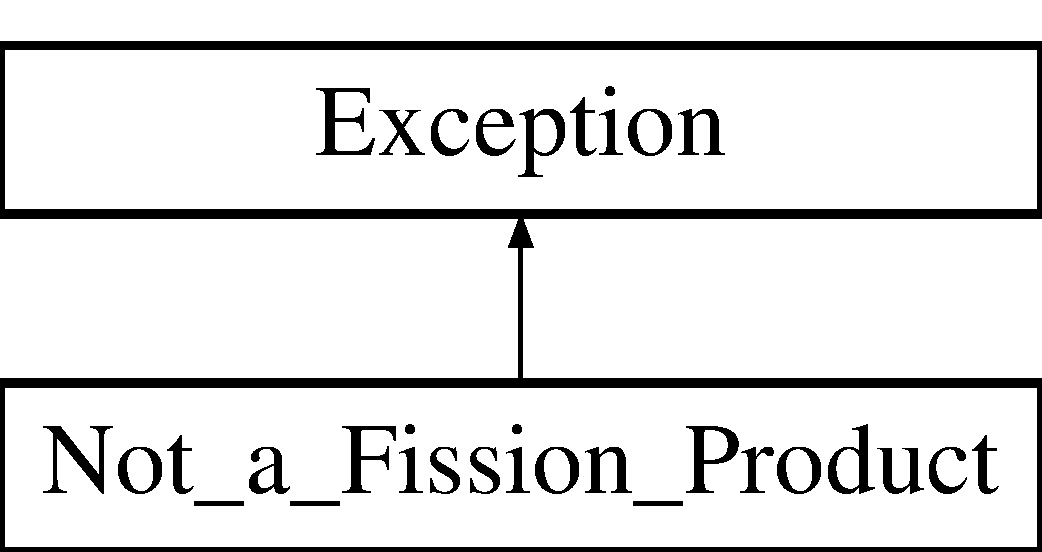
\includegraphics[height=2.000000cm]{classopenbu_1_1passport_1_1_not__a___fission___product}
\end{center}
\end{figure}


\doxysubsection{Detailed Description}
\begin{DoxyVerb}Raise when the user tries to set fission yields for a non fission product nuclide \end{DoxyVerb}
 

The documentation for this class was generated from the following file\+:\begin{DoxyCompactItemize}
\item 
passport.\+py\end{DoxyCompactItemize}

\hypertarget{classopenbu_1_1passport_1_1_nuc__xs__not__found}{}\section{Nuc\+\_\+xs\+\_\+not\+\_\+found Class Reference}
\label{classopenbu_1_1passport_1_1_nuc__xs__not__found}\index{Nuc\+\_\+xs\+\_\+not\+\_\+found@{Nuc\+\_\+xs\+\_\+not\+\_\+found}}
Inheritance diagram for Nuc\+\_\+xs\+\_\+not\+\_\+found\+:\begin{figure}[H]
\begin{center}
\leavevmode
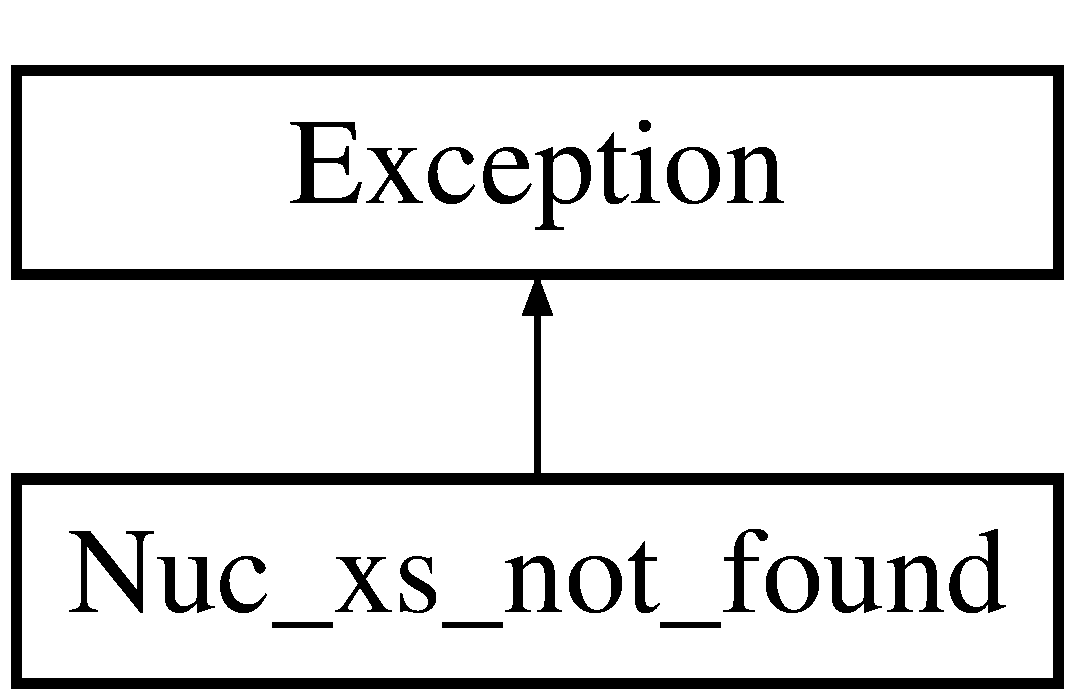
\includegraphics[height=2.000000cm]{classopenbu_1_1passport_1_1_nuc__xs__not__found}
\end{center}
\end{figure}


\subsection{Detailed Description}
\begin{DoxyVerb}Raise when the user requests a cross-sections of a nuclide that is not in the nuclide set \end{DoxyVerb}
 

The documentation for this class was generated from the following file\+:\begin{DoxyCompactItemize}
\item 
/\+Users/mouginot/work/app/\+Open\+B\+U/openbu/\mbox{\hyperlink{passport_8py}{passport.\+py}}\end{DoxyCompactItemize}

\hypertarget{classopenbu_1_1passlist_1_1_nuc__xs__not__found}{}\section{Nuc\+\_\+xs\+\_\+not\+\_\+found Class Reference}
\label{classopenbu_1_1passlist_1_1_nuc__xs__not__found}\index{Nuc\+\_\+xs\+\_\+not\+\_\+found@{Nuc\+\_\+xs\+\_\+not\+\_\+found}}
Inheritance diagram for Nuc\+\_\+xs\+\_\+not\+\_\+found\+:\begin{figure}[H]
\begin{center}
\leavevmode
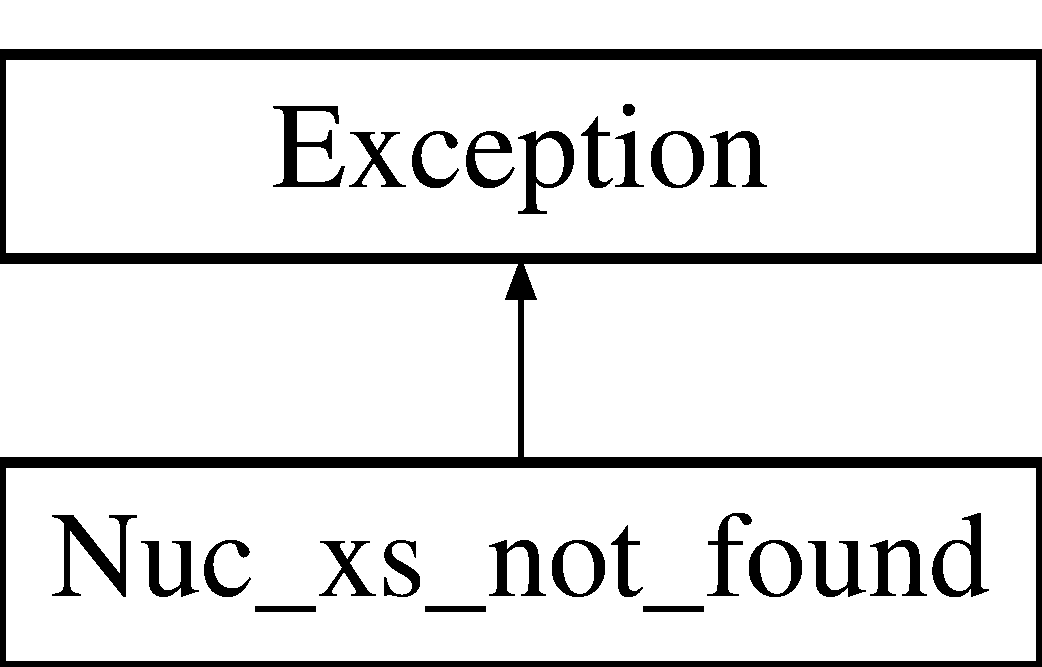
\includegraphics[height=2.000000cm]{classopenbu_1_1passlist_1_1_nuc__xs__not__found}
\end{center}
\end{figure}


\subsection{Detailed Description}
\begin{DoxyVerb}Raise when the user requests a cross-sections of a nuclide that is not in the nuclide set \end{DoxyVerb}
 

The documentation for this class was generated from the following file\+:\begin{DoxyCompactItemize}
\item 
/\+Users/mouginot/work/app/\+Open\+B\+U/openbu/\mbox{\hyperlink{passlist_8py}{passlist.\+py}}\end{DoxyCompactItemize}

\hypertarget{classopenbu_1_1cell_1_1_nucl__set__not__in___lib__nucl}{}\section{Nucl\+\_\+set\+\_\+not\+\_\+in\+\_\+\+Lib\+\_\+nucl Class Reference}
\label{classopenbu_1_1cell_1_1_nucl__set__not__in___lib__nucl}\index{Nucl\+\_\+set\+\_\+not\+\_\+in\+\_\+\+Lib\+\_\+nucl@{Nucl\+\_\+set\+\_\+not\+\_\+in\+\_\+\+Lib\+\_\+nucl}}
Inheritance diagram for Nucl\+\_\+set\+\_\+not\+\_\+in\+\_\+\+Lib\+\_\+nucl\+:\begin{figure}[H]
\begin{center}
\leavevmode
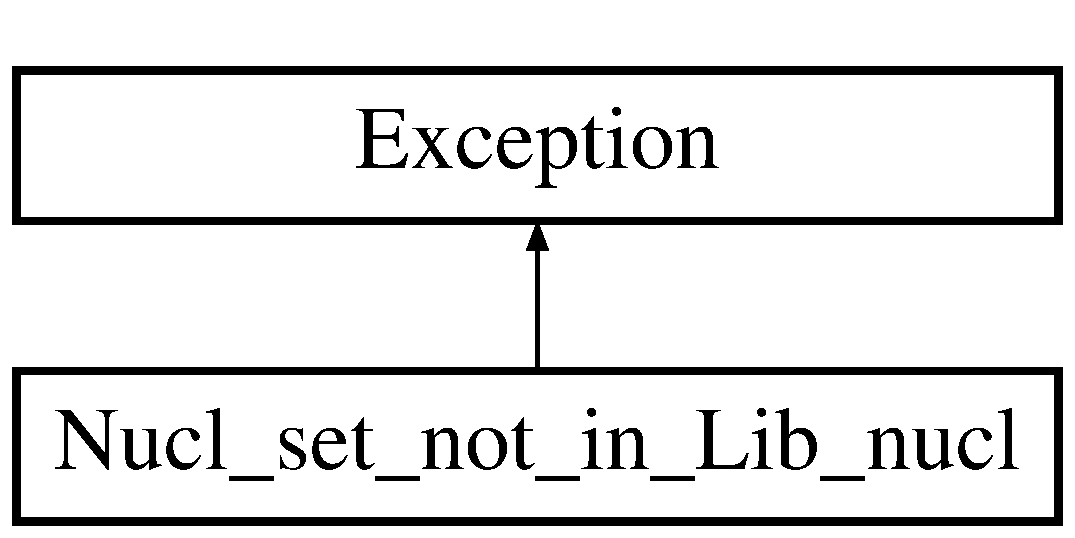
\includegraphics[height=2.000000cm]{classopenbu_1_1cell_1_1_nucl__set__not__in___lib__nucl}
\end{center}
\end{figure}


\subsection{Detailed Description}
\begin{DoxyVerb}Raise when the user forgot to set the initial nuclide of the cell and tries to burn cell\end{DoxyVerb}
 

The documentation for this class was generated from the following file\+:\begin{DoxyCompactItemize}
\item 
/\+Users/mouginot/work/app/\+Open\+B\+U/openbu/cell.\+py\end{DoxyCompactItemize}

\hypertarget{classopenbu_1_1cell_1_1_nuclide__list__redundant}{}\section{Nuclide\+\_\+list\+\_\+redundant Class Reference}
\label{classopenbu_1_1cell_1_1_nuclide__list__redundant}\index{Nuclide\+\_\+list\+\_\+redundant@{Nuclide\+\_\+list\+\_\+redundant}}
Inheritance diagram for Nuclide\+\_\+list\+\_\+redundant\+:\begin{figure}[H]
\begin{center}
\leavevmode
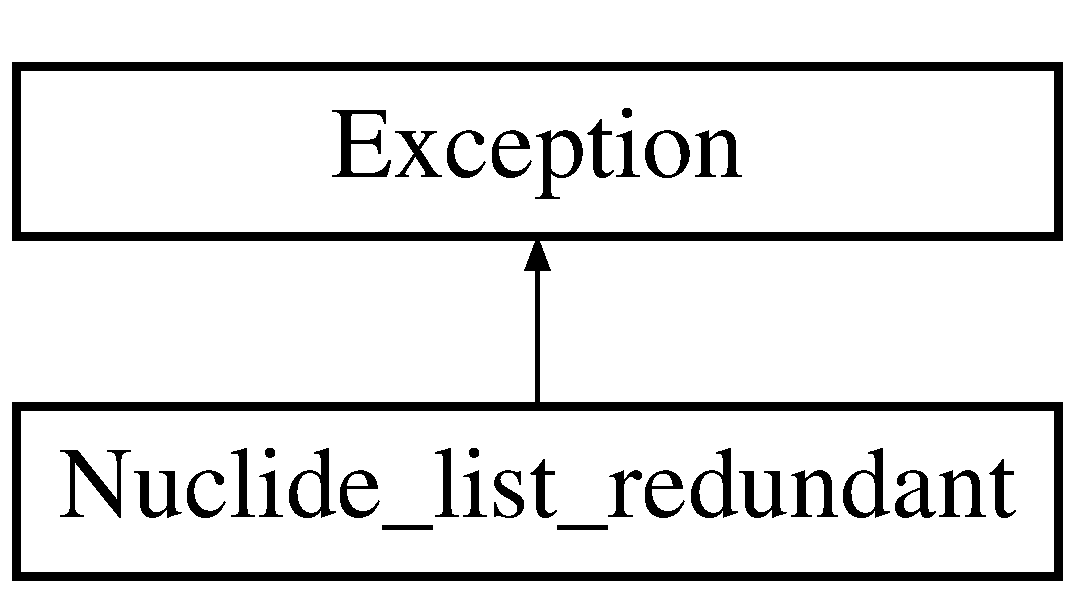
\includegraphics[height=2.000000cm]{classopenbu_1_1cell_1_1_nuclide__list__redundant}
\end{center}
\end{figure}


The documentation for this class was generated from the following file\+:\begin{DoxyCompactItemize}
\item 
/\+Users/mouginot/work/app/\+Open\+B\+U/openbu/\mbox{\hyperlink{cell_8py}{cell.\+py}}\end{DoxyCompactItemize}

\hypertarget{classopenbu_1_1passlist_1_1_passlist}{}\doxysection{Passlist Class Reference}
\label{classopenbu_1_1passlist_1_1_passlist}\index{Passlist@{Passlist}}
Inheritance diagram for Passlist\+:\begin{figure}[H]
\begin{center}
\leavevmode
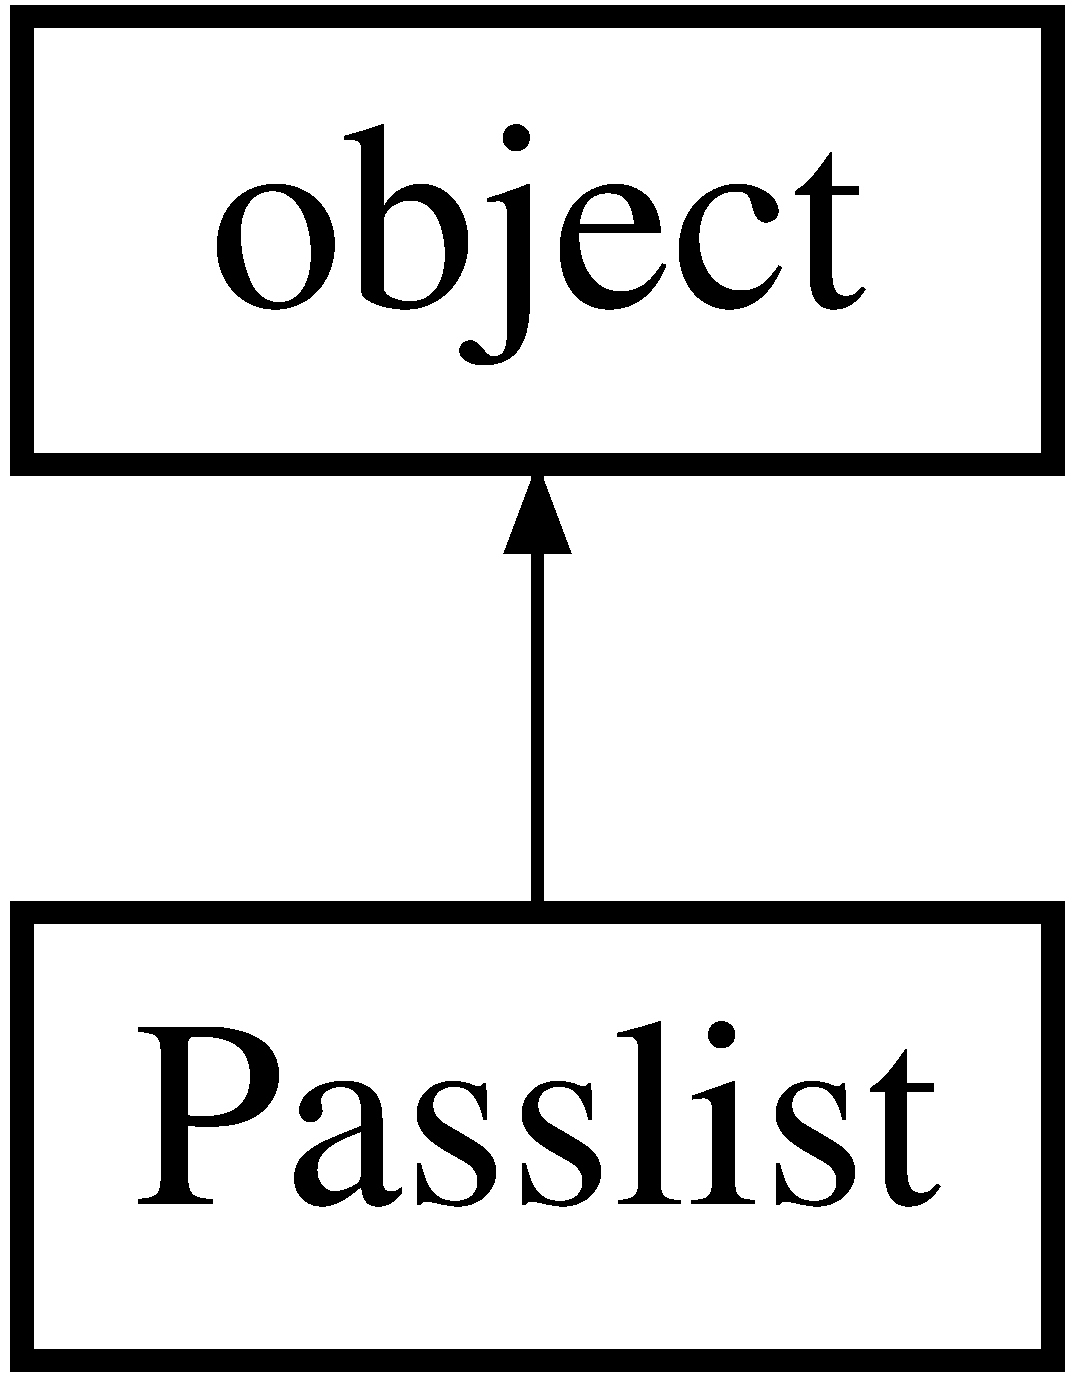
\includegraphics[height=2.000000cm]{classopenbu_1_1passlist_1_1_passlist}
\end{center}
\end{figure}
\doxysubsection*{Public Member Functions}
\doxysubsection*{Private Member Functions}
\doxysubsection*{Private Attributes}


\doxysubsection{Member Function Documentation}
\mbox{\Hypertarget{classopenbu_1_1passlist_1_1_passlist_a8c7ed2f12d3dbb3dd307013850e75afd}\label{classopenbu_1_1passlist_1_1_passlist_a8c7ed2f12d3dbb3dd307013850e75afd}} 
\index{Passlist@{Passlist}!\_get\_name\_passport\_dict@{\_get\_name\_passport\_dict}}
\index{\_get\_name\_passport\_dict@{\_get\_name\_passport\_dict}!Passlist@{Passlist}}
\doxysubsubsection{\texorpdfstring{\_get\_name\_passport\_dict()}{\_get\_name\_passport\_dict()}}
{\footnotesize\ttfamily def \+\_\+get\+\_\+name\+\_\+passport\+\_\+dict (\begin{DoxyParamCaption}\item[{}]{self }\end{DoxyParamCaption})\hspace{0.3cm}{\ttfamily [private]}}

\begin{DoxyVerb}Convert the list of passport into a dictionnary of passports where entries are the zamid of the nuclides\end{DoxyVerb}
 \mbox{\Hypertarget{classopenbu_1_1passlist_1_1_passlist_ac9b957ad1a1f7a2afccc7c7223110387}\label{classopenbu_1_1passlist_1_1_passlist_ac9b957ad1a1f7a2afccc7c7223110387}} 
\index{Passlist@{Passlist}!\_get\_zamid\_passport\_dict@{\_get\_zamid\_passport\_dict}}
\index{\_get\_zamid\_passport\_dict@{\_get\_zamid\_passport\_dict}!Passlist@{Passlist}}
\doxysubsubsection{\texorpdfstring{\_get\_zamid\_passport\_dict()}{\_get\_zamid\_passport\_dict()}}
{\footnotesize\ttfamily def \+\_\+get\+\_\+zamid\+\_\+passport\+\_\+dict (\begin{DoxyParamCaption}\item[{}]{self }\end{DoxyParamCaption})\hspace{0.3cm}{\ttfamily [private]}}

\begin{DoxyVerb}Convert the list of passport into a dictionnary of passports where entries are the zamid of the nuclides\end{DoxyVerb}
 \mbox{\Hypertarget{classopenbu_1_1passlist_1_1_passlist_a2eec6817afb9bc29c4c86d97cdb56947}\label{classopenbu_1_1passlist_1_1_passlist_a2eec6817afb9bc29c4c86d97cdb56947}} 
\index{Passlist@{Passlist}!\_overwrite\_xs@{\_overwrite\_xs}}
\index{\_overwrite\_xs@{\_overwrite\_xs}!Passlist@{Passlist}}
\doxysubsubsection{\texorpdfstring{\_overwrite\_xs()}{\_overwrite\_xs()}}
{\footnotesize\ttfamily def \+\_\+overwrite\+\_\+xs (\begin{DoxyParamCaption}\item[{}]{self,  }\item[{}]{xs\+\_\+dict }\end{DoxyParamCaption})\hspace{0.3cm}{\ttfamily [private]}}

\begin{DoxyVerb}Read and set the cross sections for each nuclide in the passports list\end{DoxyVerb}
 \mbox{\Hypertarget{classopenbu_1_1passlist_1_1_passlist_a4bf49923534fe53d939d4face28cf0f0}\label{classopenbu_1_1passlist_1_1_passlist_a4bf49923534fe53d939d4face28cf0f0}} 
\index{Passlist@{Passlist}!\_set\_decay@{\_set\_decay}}
\index{\_set\_decay@{\_set\_decay}!Passlist@{Passlist}}
\doxysubsubsection{\texorpdfstring{\_set\_decay()}{\_set\_decay()}}
{\footnotesize\ttfamily def \+\_\+set\+\_\+decay (\begin{DoxyParamCaption}\item[{}]{self,  }\item[{}]{decay\+\_\+lib\+\_\+b,  }\item[{}]{decay\+\_\+lib\+\_\+a }\end{DoxyParamCaption})\hspace{0.3cm}{\ttfamily [private]}}

\begin{DoxyVerb}Read and set the decay constants for each nuclide in the passports list\end{DoxyVerb}
 \mbox{\Hypertarget{classopenbu_1_1passlist_1_1_passlist_a29902b392d57e73485c65bfbfdff566e}\label{classopenbu_1_1passlist_1_1_passlist_a29902b392d57e73485c65bfbfdff566e}} 
\index{Passlist@{Passlist}!\_set\_fy@{\_set\_fy}}
\index{\_set\_fy@{\_set\_fy}!Passlist@{Passlist}}
\doxysubsubsection{\texorpdfstring{\_set\_fy()}{\_set\_fy()}}
{\footnotesize\ttfamily def \+\_\+set\+\_\+fy (\begin{DoxyParamCaption}\item[{}]{self,  }\item[{}]{fy\+\_\+dict }\end{DoxyParamCaption})\hspace{0.3cm}{\ttfamily [private]}}

\begin{DoxyVerb}Read and set the fission yields for fission products in the passports list\end{DoxyVerb}
 \mbox{\Hypertarget{classopenbu_1_1passlist_1_1_passlist_a956fb79a1bafe4c9a4f831ed4be4005c}\label{classopenbu_1_1passlist_1_1_passlist_a956fb79a1bafe4c9a4f831ed4be4005c}} 
\index{Passlist@{Passlist}!\_set\_mass@{\_set\_mass}}
\index{\_set\_mass@{\_set\_mass}!Passlist@{Passlist}}
\doxysubsubsection{\texorpdfstring{\_set\_mass()}{\_set\_mass()}}
{\footnotesize\ttfamily def \+\_\+set\+\_\+mass (\begin{DoxyParamCaption}\item[{}]{self,  }\item[{}]{passport\+\_\+list }\end{DoxyParamCaption})\hspace{0.3cm}{\ttfamily [private]}}

\begin{DoxyVerb}Read and set the atomic mass for each nuclide in the passports list\end{DoxyVerb}
 \mbox{\Hypertarget{classopenbu_1_1passlist_1_1_passlist_aa45dff0e552a6f90aef82cfd5c0691b9}\label{classopenbu_1_1passlist_1_1_passlist_aa45dff0e552a6f90aef82cfd5c0691b9}} 
\index{Passlist@{Passlist}!\_set\_xs@{\_set\_xs}}
\index{\_set\_xs@{\_set\_xs}!Passlist@{Passlist}}
\doxysubsubsection{\texorpdfstring{\_set\_xs()}{\_set\_xs()}}
{\footnotesize\ttfamily def \+\_\+set\+\_\+xs (\begin{DoxyParamCaption}\item[{}]{self,  }\item[{}]{xs\+\_\+dict }\end{DoxyParamCaption})\hspace{0.3cm}{\ttfamily [private]}}

\begin{DoxyVerb}Read and set the cross sections for each nuclide in the passports list\end{DoxyVerb}
 

The documentation for this class was generated from the following file\+:\begin{DoxyCompactItemize}
\item 
passlist.\+py\end{DoxyCompactItemize}

\hypertarget{classopenbu_1_1cell_1_1_passlist__not__defined}{}\section{Passlist\+\_\+not\+\_\+defined Class Reference}
\label{classopenbu_1_1cell_1_1_passlist__not__defined}\index{Passlist\+\_\+not\+\_\+defined@{Passlist\+\_\+not\+\_\+defined}}
Inheritance diagram for Passlist\+\_\+not\+\_\+defined\+:\begin{figure}[H]
\begin{center}
\leavevmode
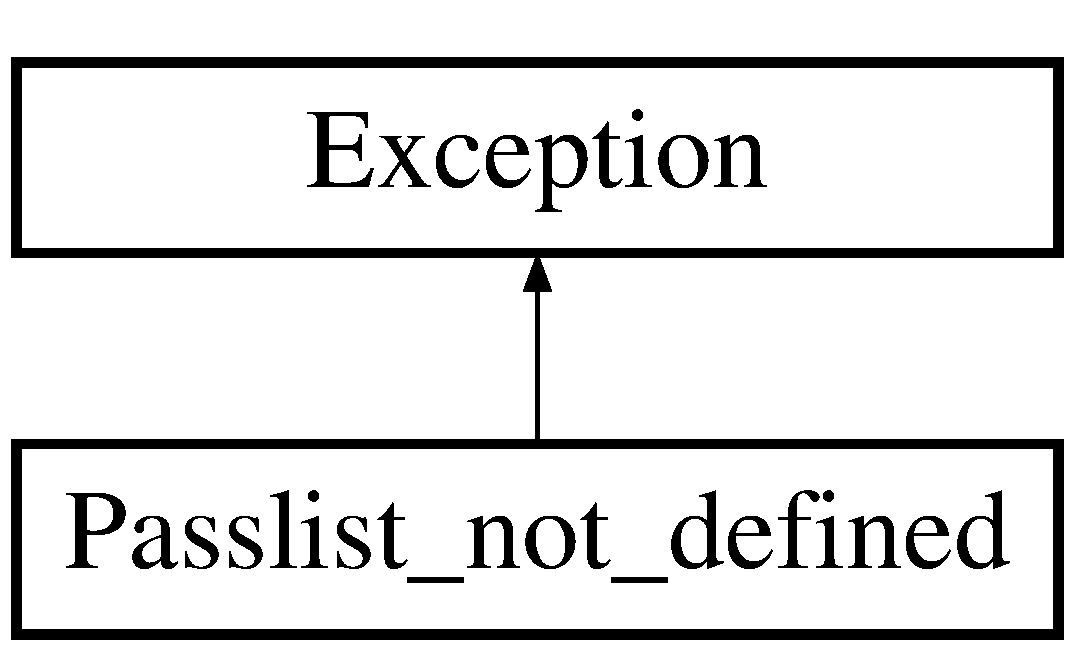
\includegraphics[height=2.000000cm]{classopenbu_1_1cell_1_1_passlist__not__defined}
\end{center}
\end{figure}


\subsection{Detailed Description}
\begin{DoxyVerb}Raise when the user forgot to defined passlist for a cell\end{DoxyVerb}
 

The documentation for this class was generated from the following file\+:\begin{DoxyCompactItemize}
\item 
/\+Users/mouginot/work/app/\+Open\+B\+U/openbu/cell.\+py\end{DoxyCompactItemize}

\hypertarget{classopenbu_1_1passport_1_1_passport}{}\doxysection{Passport Class Reference}
\label{classopenbu_1_1passport_1_1_passport}\index{Passport@{Passport}}
Inheritance diagram for Passport\+:\begin{figure}[H]
\begin{center}
\leavevmode
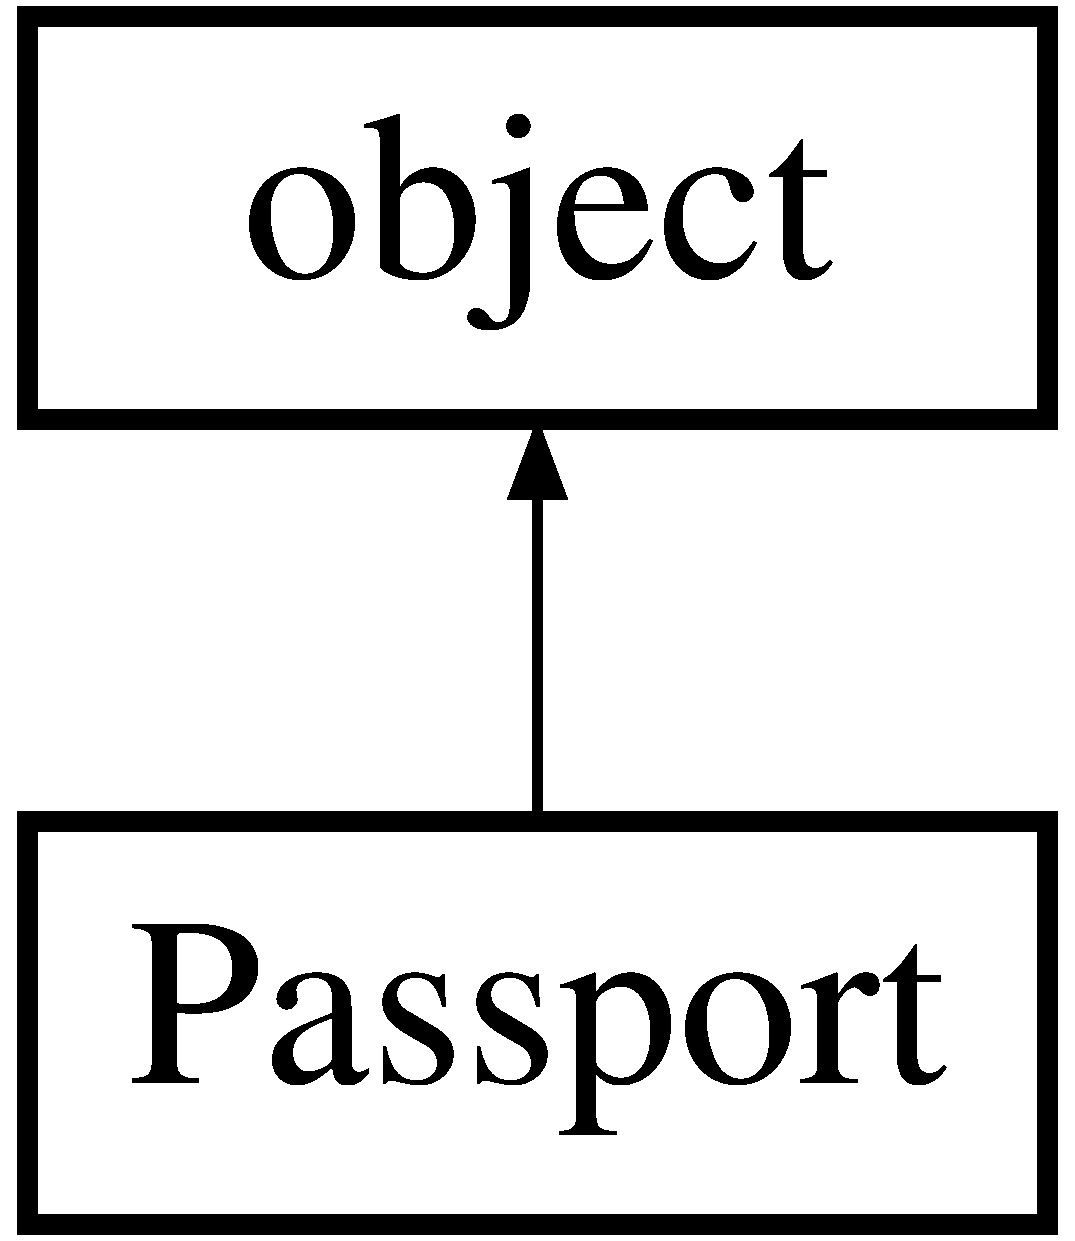
\includegraphics[height=2.000000cm]{classopenbu_1_1passport_1_1_passport}
\end{center}
\end{figure}
\doxysubsection*{Public Member Functions}
\doxysubsection*{Public Attributes}
\doxysubsection*{Private Member Functions}
\doxysubsection*{Private Attributes}
\doxysubsection*{Static Private Attributes}


\doxysubsection{Detailed Description}
\begin{DoxyVerb}passport stores all the relevant data of indivudual nuclides and offers methods to extract information on them

   The passport class is individually instantiated for each nuclide. It contains two types of information: constant and variable data.
   Constant data, such as the atomic mass, decay constant or the element's family (actinide, fission product) do not change over the course of a simulation.
   Variable data such as cross sections or fission yields do vary during a simulation and need thus to be updated regularly during a simulation.
   Some of the data are created at the time of the instantiation of the class for a nuclide such as the element's family or the nuclide's
   neutron reaction daughters. Other type of data, typically large in size such as cross sections and decay constants, are to be explicitly set or loaded.
   A setter method will enable any script that reads the data source to set this data for the passport of a specific nuclide. This is the method used within
   the code of Open-Burnup to set the data for a list of passports. The other way to explicitly set the data is to use the loader method. This method will
   go to the data source itself, read the data and set it for the passport of a specific nuclide. This method is envision to be used by the user as a
   user-friendly way to get information on individual nuclides.

   Attributes:
       * **decay_a:** returns the absolute value of the decay constants of the nuclide
       * **decay_b:** returns the percent fraction value of the decay constants of the nuclide
       * **fy:** returns the value of fission yields in percent
       * **mass:** returns the atomic mass of the nuclide
       * **xs:** returns the absolute value of cross sections for the nuclide
       * **FAM:** returns the family group name of the nuclide
       * **xs_relatives:** returns neutron reaction's daughter nuclides' id
       * **decay_relatives:** returns decay reaction's daughter nuclides' id

   Methods:
       * **set_mass():** set the atomic mass of the nuclide
       * **set_decay():** set the decay constants (both absolute values and percent fractions) of the nuclide
       * **set_xs():** set the cross sections of the nuclide
       * **set_fy():** set the fission yields of the nuclide
       * **load_mass():** load the atomic mass of the nuclide
       * **load_decay():** load the decay constants (both absolute values and percent fractions) of the nuclide
       * **load_mass():** load the cross sections of the nuclide
       * **load_mass():** load the fission yields of the nuclide
       * **get__zamid():** returns the zzaaam id of the nuclide
       * **get_nuc_name():** returns the name of the nuclide\end{DoxyVerb}
 

\doxysubsection{Member Function Documentation}
\mbox{\Hypertarget{classopenbu_1_1passport_1_1_passport_a1d13e38c1df92265a6b65961522978e9}\label{classopenbu_1_1passport_1_1_passport_a1d13e38c1df92265a6b65961522978e9}} 
\index{Passport@{Passport}!\_set\_initial\_dens@{\_set\_initial\_dens}}
\index{\_set\_initial\_dens@{\_set\_initial\_dens}!Passport@{Passport}}
\doxysubsubsection{\texorpdfstring{\_set\_initial\_dens()}{\_set\_initial\_dens()}}
{\footnotesize\ttfamily def \+\_\+set\+\_\+initial\+\_\+dens (\begin{DoxyParamCaption}\item[{}]{self,  }\item[{}]{new\+\_\+dens }\end{DoxyParamCaption})\hspace{0.3cm}{\ttfamily [private]}}

\begin{DoxyVerb}set new dens to current dens and append to dens_seqor\end{DoxyVerb}
 \mbox{\Hypertarget{classopenbu_1_1passport_1_1_passport_a3f7ead3ec8497f2dea2c5b4a8efb3064}\label{classopenbu_1_1passport_1_1_passport_a3f7ead3ec8497f2dea2c5b4a8efb3064}} 
\index{Passport@{Passport}!\_set\_state@{\_set\_state}}
\index{\_set\_state@{\_set\_state}!Passport@{Passport}}
\doxysubsubsection{\texorpdfstring{\_set\_state()}{\_set\_state()}}
{\footnotesize\ttfamily def \+\_\+set\+\_\+state (\begin{DoxyParamCaption}\item[{}]{self }\end{DoxyParamCaption})\hspace{0.3cm}{\ttfamily [private]}}

\begin{DoxyVerb}Returns the state of the nuclide (excited or ground state)\end{DoxyVerb}
 \mbox{\Hypertarget{classopenbu_1_1passport_1_1_passport_aae6f90e1f0871cddaad54d66a6bd6529}\label{classopenbu_1_1passport_1_1_passport_aae6f90e1f0871cddaad54d66a6bd6529}} 
\index{Passport@{Passport}!current\_dens@{current\_dens}}
\index{current\_dens@{current\_dens}!Passport@{Passport}}
\doxysubsubsection{\texorpdfstring{current\_dens()}{current\_dens()}\hspace{0.1cm}{\footnotesize\ttfamily [1/2]}}
{\footnotesize\ttfamily def current\+\_\+dens (\begin{DoxyParamCaption}\item[{}]{self }\end{DoxyParamCaption})}

\begin{DoxyVerb}Returns the density of the nuclide in atom per cm^3\end{DoxyVerb}
 \mbox{\Hypertarget{classopenbu_1_1passport_1_1_passport_a2e640e060087e64c0e938f17b6c3653e}\label{classopenbu_1_1passport_1_1_passport_a2e640e060087e64c0e938f17b6c3653e}} 
\index{Passport@{Passport}!current\_dens@{current\_dens}}
\index{current\_dens@{current\_dens}!Passport@{Passport}}
\doxysubsubsection{\texorpdfstring{current\_dens()}{current\_dens()}\hspace{0.1cm}{\footnotesize\ttfamily [2/2]}}
{\footnotesize\ttfamily def current\+\_\+dens (\begin{DoxyParamCaption}\item[{}]{self,  }\item[{}]{new\+\_\+dens }\end{DoxyParamCaption})}

\begin{DoxyVerb}set the density of the nuclide in atom per cm^3\end{DoxyVerb}
 \mbox{\Hypertarget{classopenbu_1_1passport_1_1_passport_a555c209d9b1ea0fcc30cb14a259342f4}\label{classopenbu_1_1passport_1_1_passport_a555c209d9b1ea0fcc30cb14a259342f4}} 
\index{Passport@{Passport}!current\_xs@{current\_xs}}
\index{current\_xs@{current\_xs}!Passport@{Passport}}
\doxysubsubsection{\texorpdfstring{current\_xs()}{current\_xs()}}
{\footnotesize\ttfamily def current\+\_\+xs (\begin{DoxyParamCaption}\item[{}]{self }\end{DoxyParamCaption})}

\begin{DoxyVerb}Returns the cross sections data of the nuclide\end{DoxyVerb}
 \mbox{\Hypertarget{classopenbu_1_1passport_1_1_passport_ab9d903431dc1a815d57cb09912e41e58}\label{classopenbu_1_1passport_1_1_passport_ab9d903431dc1a815d57cb09912e41e58}} 
\index{Passport@{Passport}!decay\_a@{decay\_a}}
\index{decay\_a@{decay\_a}!Passport@{Passport}}
\doxysubsubsection{\texorpdfstring{decay\_a()}{decay\_a()}}
{\footnotesize\ttfamily def decay\+\_\+a (\begin{DoxyParamCaption}\item[{}]{self }\end{DoxyParamCaption})}

\begin{DoxyVerb}Returns the absolute values of the decay constant of the nuclide\end{DoxyVerb}
 \mbox{\Hypertarget{classopenbu_1_1passport_1_1_passport_ade7165602b6bcdee1ed9b7256170379b}\label{classopenbu_1_1passport_1_1_passport_ade7165602b6bcdee1ed9b7256170379b}} 
\index{Passport@{Passport}!decay\_b@{decay\_b}}
\index{decay\_b@{decay\_b}!Passport@{Passport}}
\doxysubsubsection{\texorpdfstring{decay\_b()}{decay\_b()}}
{\footnotesize\ttfamily def decay\+\_\+b (\begin{DoxyParamCaption}\item[{}]{self }\end{DoxyParamCaption})}

\begin{DoxyVerb}Returns the fraction percent values of the decay constant of the nuclide\end{DoxyVerb}
 \mbox{\Hypertarget{classopenbu_1_1passport_1_1_passport_afe7a50b1cfeb99651932d201b32e1eac}\label{classopenbu_1_1passport_1_1_passport_afe7a50b1cfeb99651932d201b32e1eac}} 
\index{Passport@{Passport}!decay\_child@{decay\_child}}
\index{decay\_child@{decay\_child}!Passport@{Passport}}
\doxysubsubsection{\texorpdfstring{decay\_child()}{decay\_child()}}
{\footnotesize\ttfamily def decay\+\_\+child (\begin{DoxyParamCaption}\item[{}]{self }\end{DoxyParamCaption})}

\begin{DoxyVerb}Returns the decay reactions' daughter products\end{DoxyVerb}
 \mbox{\Hypertarget{classopenbu_1_1passport_1_1_passport_a036610ac850c29ffb1e5172cff7c679a}\label{classopenbu_1_1passport_1_1_passport_a036610ac850c29ffb1e5172cff7c679a}} 
\index{Passport@{Passport}!decay\_parent@{decay\_parent}}
\index{decay\_parent@{decay\_parent}!Passport@{Passport}}
\doxysubsubsection{\texorpdfstring{decay\_parent()}{decay\_parent()}}
{\footnotesize\ttfamily def decay\+\_\+parent (\begin{DoxyParamCaption}\item[{}]{self }\end{DoxyParamCaption})}

\begin{DoxyVerb}Returns the decay reactions' daughter products\end{DoxyVerb}
 \mbox{\Hypertarget{classopenbu_1_1passport_1_1_passport_a8b75ace3008810461600cc7df511303b}\label{classopenbu_1_1passport_1_1_passport_a8b75ace3008810461600cc7df511303b}} 
\index{Passport@{Passport}!fy@{fy}}
\index{fy@{fy}!Passport@{Passport}}
\doxysubsubsection{\texorpdfstring{fy()}{fy()}}
{\footnotesize\ttfamily def fy (\begin{DoxyParamCaption}\item[{}]{self }\end{DoxyParamCaption})}

\begin{DoxyVerb}Returns the fission yields data in percent\end{DoxyVerb}
 \mbox{\Hypertarget{classopenbu_1_1passport_1_1_passport_aa1146a83b02f1768536bf28e3f5776ea}\label{classopenbu_1_1passport_1_1_passport_aa1146a83b02f1768536bf28e3f5776ea}} 
\index{Passport@{Passport}!get\_a@{get\_a}}
\index{get\_a@{get\_a}!Passport@{Passport}}
\doxysubsubsection{\texorpdfstring{get\_a()}{get\_a()}}
{\footnotesize\ttfamily def get\+\_\+a (\begin{DoxyParamCaption}\item[{}]{self }\end{DoxyParamCaption})}

\begin{DoxyVerb}Returns the mass number of the nuclide\end{DoxyVerb}
 \mbox{\Hypertarget{classopenbu_1_1passport_1_1_passport_aa75b75b6a9d2a68e6a592e7353044edb}\label{classopenbu_1_1passport_1_1_passport_aa75b75b6a9d2a68e6a592e7353044edb}} 
\index{Passport@{Passport}!get\_z@{get\_z}}
\index{get\_z@{get\_z}!Passport@{Passport}}
\doxysubsubsection{\texorpdfstring{get\_z()}{get\_z()}}
{\footnotesize\ttfamily def get\+\_\+z (\begin{DoxyParamCaption}\item[{}]{self }\end{DoxyParamCaption})}

\begin{DoxyVerb}Returns the atomic number of the nuclide\end{DoxyVerb}
 \mbox{\Hypertarget{classopenbu_1_1passport_1_1_passport_ab6f7c3af79510d2bf012aa1a483a6cf8}\label{classopenbu_1_1passport_1_1_passport_ab6f7c3af79510d2bf012aa1a483a6cf8}} 
\index{Passport@{Passport}!load\_decay@{load\_decay}}
\index{load\_decay@{load\_decay}!Passport@{Passport}}
\doxysubsubsection{\texorpdfstring{load\_decay()}{load\_decay()}}
{\footnotesize\ttfamily def load\+\_\+decay (\begin{DoxyParamCaption}\item[{}]{self }\end{DoxyParamCaption})}

\begin{DoxyVerb}Load the decay constant value of the nuclide

This method directly fetches the decay constant values from the source data and automatically set
of the passport object\end{DoxyVerb}
 \mbox{\Hypertarget{classopenbu_1_1passport_1_1_passport_a3fd9b285c12428f2f1021f6fa498d27b}\label{classopenbu_1_1passport_1_1_passport_a3fd9b285c12428f2f1021f6fa498d27b}} 
\index{Passport@{Passport}!load\_fy@{load\_fy}}
\index{load\_fy@{load\_fy}!Passport@{Passport}}
\doxysubsubsection{\texorpdfstring{load\_fy()}{load\_fy()}}
{\footnotesize\ttfamily def load\+\_\+fy (\begin{DoxyParamCaption}\item[{}]{self }\end{DoxyParamCaption})}

\begin{DoxyVerb}Load the fission yields data of the nuclide

This method directly fetches the fission yields data from the source data and automatically set
of the passport object

If the nuclide for which the fission yields data are being loaded is not a fission product,
the error *Not_a_Fission_Product* will be raised\end{DoxyVerb}
 \mbox{\Hypertarget{classopenbu_1_1passport_1_1_passport_a791d705e172d19c0cdc181960287cc78}\label{classopenbu_1_1passport_1_1_passport_a791d705e172d19c0cdc181960287cc78}} 
\index{Passport@{Passport}!load\_mass@{load\_mass}}
\index{load\_mass@{load\_mass}!Passport@{Passport}}
\doxysubsubsection{\texorpdfstring{load\_mass()}{load\_mass()}}
{\footnotesize\ttfamily def load\+\_\+mass (\begin{DoxyParamCaption}\item[{}]{self }\end{DoxyParamCaption})}

\begin{DoxyVerb}Load the atomic mass of the nuclide in gram

This method directly fetches the atomic mass from the source data and automatically set
of the passport object\end{DoxyVerb}
 \mbox{\Hypertarget{classopenbu_1_1passport_1_1_passport_a1687aea883b9cdececdb7b88b659cd5c}\label{classopenbu_1_1passport_1_1_passport_a1687aea883b9cdececdb7b88b659cd5c}} 
\index{Passport@{Passport}!load\_xs@{load\_xs}}
\index{load\_xs@{load\_xs}!Passport@{Passport}}
\doxysubsubsection{\texorpdfstring{load\_xs()}{load\_xs()}}
{\footnotesize\ttfamily def load\+\_\+xs (\begin{DoxyParamCaption}\item[{}]{self }\end{DoxyParamCaption})}

\begin{DoxyVerb}Load the cross sections data of the nuclide

This method directly fetches the cross sections data from the source data and automatically set
of the passport object\end{DoxyVerb}
 \mbox{\Hypertarget{classopenbu_1_1passport_1_1_passport_a69ae279139576858c6ca4dc9f5912717}\label{classopenbu_1_1passport_1_1_passport_a69ae279139576858c6ca4dc9f5912717}} 
\index{Passport@{Passport}!mass@{mass}}
\index{mass@{mass}!Passport@{Passport}}
\doxysubsubsection{\texorpdfstring{mass()}{mass()}}
{\footnotesize\ttfamily def mass (\begin{DoxyParamCaption}\item[{}]{self }\end{DoxyParamCaption})}

\begin{DoxyVerb}Return the atomic mass of the nuclide in gram\end{DoxyVerb}
 \mbox{\Hypertarget{classopenbu_1_1passport_1_1_passport_ae04c67eded9e7f018b551d4be5d36f2c}\label{classopenbu_1_1passport_1_1_passport_ae04c67eded9e7f018b551d4be5d36f2c}} 
\index{Passport@{Passport}!set\_decay@{set\_decay}}
\index{set\_decay@{set\_decay}!Passport@{Passport}}
\doxysubsubsection{\texorpdfstring{set\_decay()}{set\_decay()}}
{\footnotesize\ttfamily def set\+\_\+decay (\begin{DoxyParamCaption}\item[{}]{self,  }\item[{}]{decay\+\_\+a,  }\item[{}]{decay\+\_\+b }\end{DoxyParamCaption})}

\begin{DoxyVerb}Set the absolute and fracional values of the decay constant of the nuclide\end{DoxyVerb}
 \mbox{\Hypertarget{classopenbu_1_1passport_1_1_passport_af0b4eabf69455a1ace31fadfc437695b}\label{classopenbu_1_1passport_1_1_passport_af0b4eabf69455a1ace31fadfc437695b}} 
\index{Passport@{Passport}!xs\_child@{xs\_child}}
\index{xs\_child@{xs\_child}!Passport@{Passport}}
\doxysubsubsection{\texorpdfstring{xs\_child()}{xs\_child()}}
{\footnotesize\ttfamily def xs\+\_\+child (\begin{DoxyParamCaption}\item[{}]{self }\end{DoxyParamCaption})}

\begin{DoxyVerb}Returns the neutron reactions' daughter products\end{DoxyVerb}
 \mbox{\Hypertarget{classopenbu_1_1passport_1_1_passport_a0f25e060e526ebc2db82f4769504a0b4}\label{classopenbu_1_1passport_1_1_passport_a0f25e060e526ebc2db82f4769504a0b4}} 
\index{Passport@{Passport}!xs\_parent@{xs\_parent}}
\index{xs\_parent@{xs\_parent}!Passport@{Passport}}
\doxysubsubsection{\texorpdfstring{xs\_parent()}{xs\_parent()}}
{\footnotesize\ttfamily def xs\+\_\+parent (\begin{DoxyParamCaption}\item[{}]{self }\end{DoxyParamCaption})}

\begin{DoxyVerb}Returns the neutron reactions' daughter products\end{DoxyVerb}
 

The documentation for this class was generated from the following file\+:\begin{DoxyCompactItemize}
\item 
passport.\+py\end{DoxyCompactItemize}

\hypertarget{classopenbu_1_1sequence_1_1_sequence}{}\section{Sequence Class Reference}
\label{classopenbu_1_1sequence_1_1_sequence}\index{Sequence@{Sequence}}
Inheritance diagram for Sequence\+:\begin{figure}[H]
\begin{center}
\leavevmode
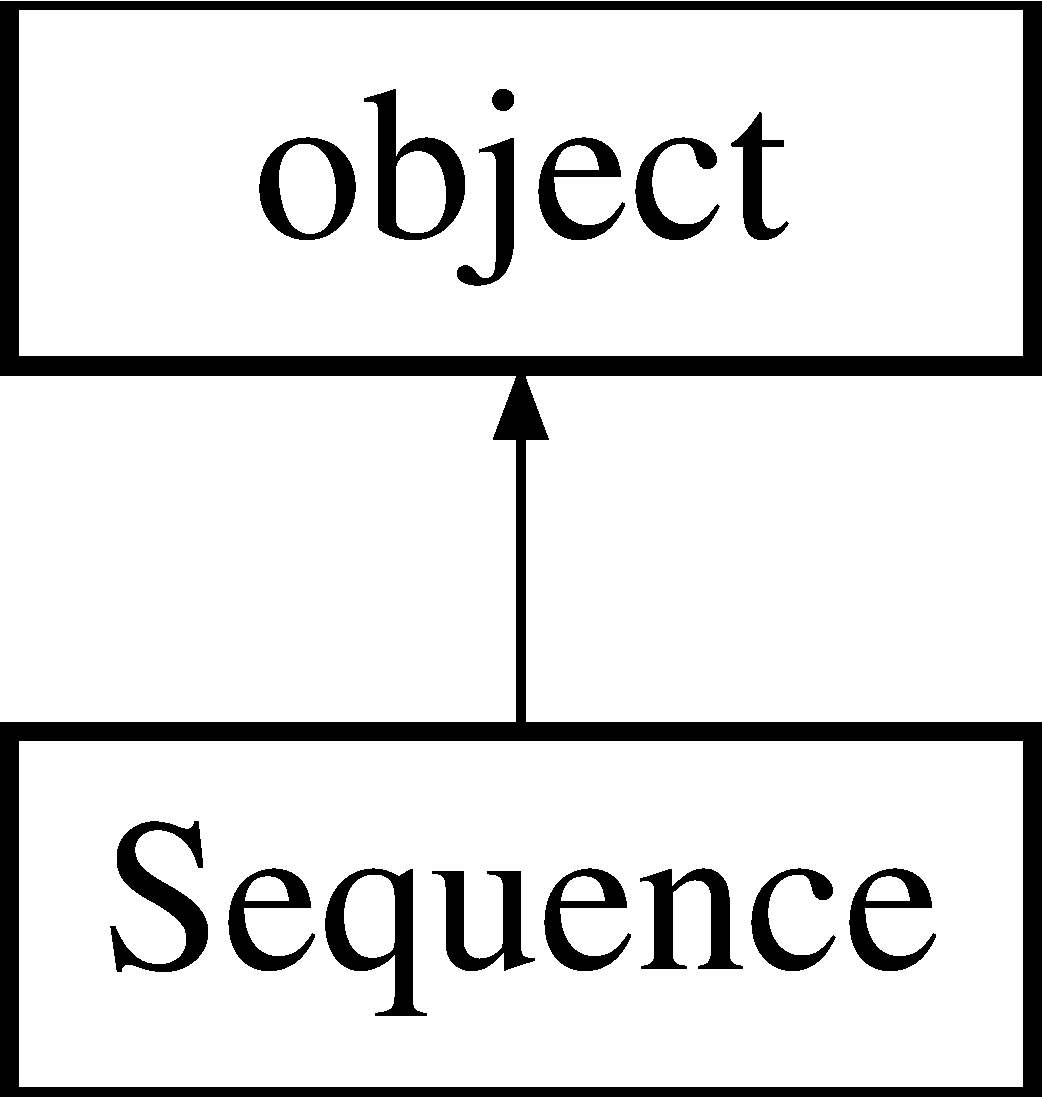
\includegraphics[height=2.000000cm]{classopenbu_1_1sequence_1_1_sequence}
\end{center}
\end{figure}
\subsection*{Public Member Functions}
\subsection*{Public Attributes}
\subsection*{Private Member Functions}
\subsection*{Private Attributes}


\subsection{Member Function Documentation}
\mbox{\Hypertarget{classopenbu_1_1sequence_1_1_sequence_aa4fed9a7ae1513bbb0db097c62569bd3}\label{classopenbu_1_1sequence_1_1_sequence_aa4fed9a7ae1513bbb0db097c62569bd3}} 
\index{openbu\+::sequence\+::\+Sequence@{openbu\+::sequence\+::\+Sequence}!\+\_\+set\+\_\+initial\+\_\+flux@{\+\_\+set\+\_\+initial\+\_\+flux}}
\index{\+\_\+set\+\_\+initial\+\_\+flux@{\+\_\+set\+\_\+initial\+\_\+flux}!openbu\+::sequence\+::\+Sequence@{openbu\+::sequence\+::\+Sequence}}
\subsubsection{\texorpdfstring{\+\_\+set\+\_\+initial\+\_\+flux()}{\_set\_initial\_flux()}}
{\footnotesize\ttfamily def \+\_\+set\+\_\+initial\+\_\+flux (\begin{DoxyParamCaption}\item[{}]{self,  }\item[{}]{new\+\_\+flux }\end{DoxyParamCaption})\hspace{0.3cm}{\ttfamily [private]}}

\begin{DoxyVerb}set new new_flux to current flux and append to flux sequence\end{DoxyVerb}
 \mbox{\Hypertarget{classopenbu_1_1sequence_1_1_sequence_a824e7bd80e4d7312e7327103b4862906}\label{classopenbu_1_1sequence_1_1_sequence_a824e7bd80e4d7312e7327103b4862906}} 
\index{openbu\+::sequence\+::\+Sequence@{openbu\+::sequence\+::\+Sequence}!\+\_\+set\+\_\+initial\+\_\+pow\+\_\+dens@{\+\_\+set\+\_\+initial\+\_\+pow\+\_\+dens}}
\index{\+\_\+set\+\_\+initial\+\_\+pow\+\_\+dens@{\+\_\+set\+\_\+initial\+\_\+pow\+\_\+dens}!openbu\+::sequence\+::\+Sequence@{openbu\+::sequence\+::\+Sequence}}
\subsubsection{\texorpdfstring{\+\_\+set\+\_\+initial\+\_\+pow\+\_\+dens()}{\_set\_initial\_pow\_dens()}}
{\footnotesize\ttfamily def \+\_\+set\+\_\+initial\+\_\+pow\+\_\+dens (\begin{DoxyParamCaption}\item[{}]{self,  }\item[{}]{new\+\_\+pow\+\_\+dens }\end{DoxyParamCaption})\hspace{0.3cm}{\ttfamily [private]}}

\begin{DoxyVerb}set new new_pow_dens to current pow_dens and append to pow_dens sequence\end{DoxyVerb}
 

The documentation for this class was generated from the following file\+:\begin{DoxyCompactItemize}
\item 
/\+Users/mouginot/work/app/\+Open\+B\+U/openbu/sequence.\+py\end{DoxyCompactItemize}

\hypertarget{classopenbu_1_1standalone_1_1_stand__alone}{}\section{Stand\+\_\+alone Class Reference}
\label{classopenbu_1_1standalone_1_1_stand__alone}\index{Stand\+\_\+alone@{Stand\+\_\+alone}}
Inheritance diagram for Stand\+\_\+alone\+:\begin{figure}[H]
\begin{center}
\leavevmode
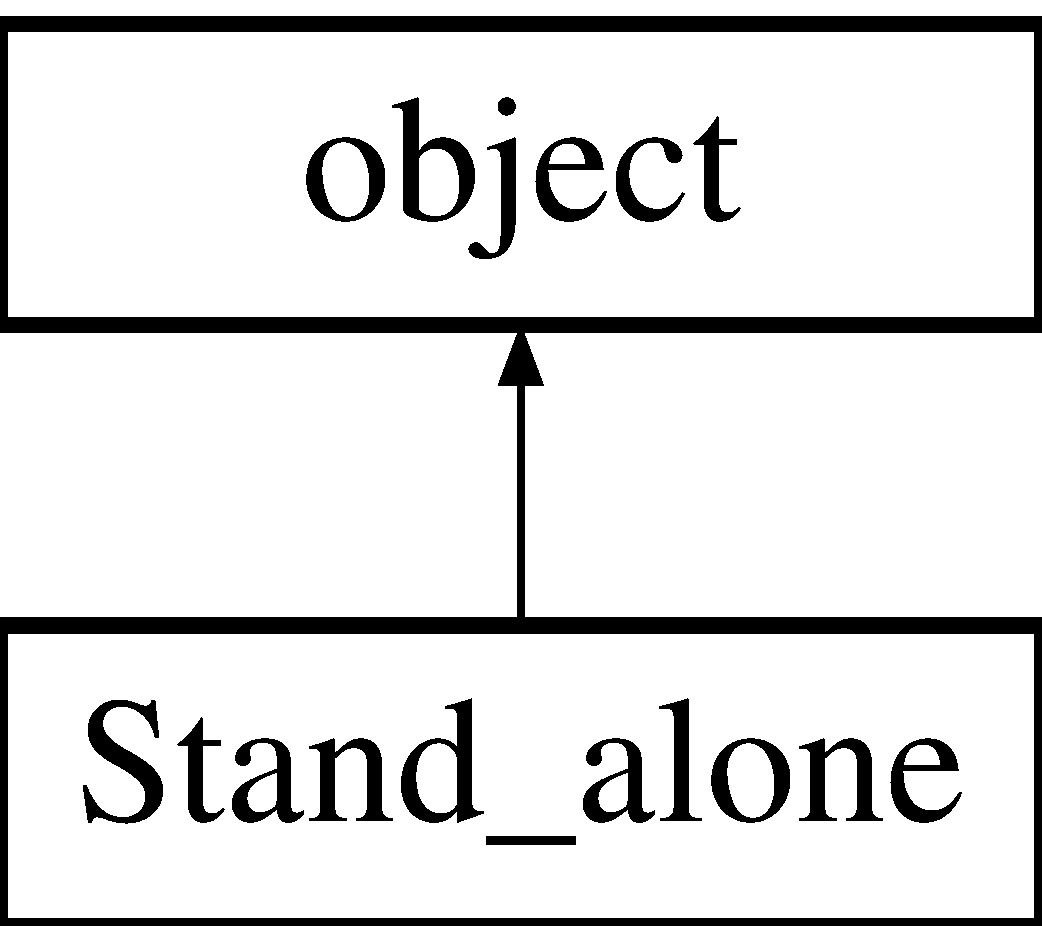
\includegraphics[height=2.000000cm]{classopenbu_1_1standalone_1_1_stand__alone}
\end{center}
\end{figure}
\subsection*{Public Member Functions}
\subsection*{Public Attributes}
\subsection*{Private Attributes}


The documentation for this class was generated from the following file\+:\begin{DoxyCompactItemize}
\item 
/\+Users/mouginot/work/app/\+Open\+B\+U/openbu/standalone.\+py\end{DoxyCompactItemize}

\hypertarget{classopenbu_1_1sequence_1_1_step__0}{}\section{Step\+\_\+0 Class Reference}
\label{classopenbu_1_1sequence_1_1_step__0}\index{Step\+\_\+0@{Step\+\_\+0}}
Inheritance diagram for Step\+\_\+0\+:\begin{figure}[H]
\begin{center}
\leavevmode
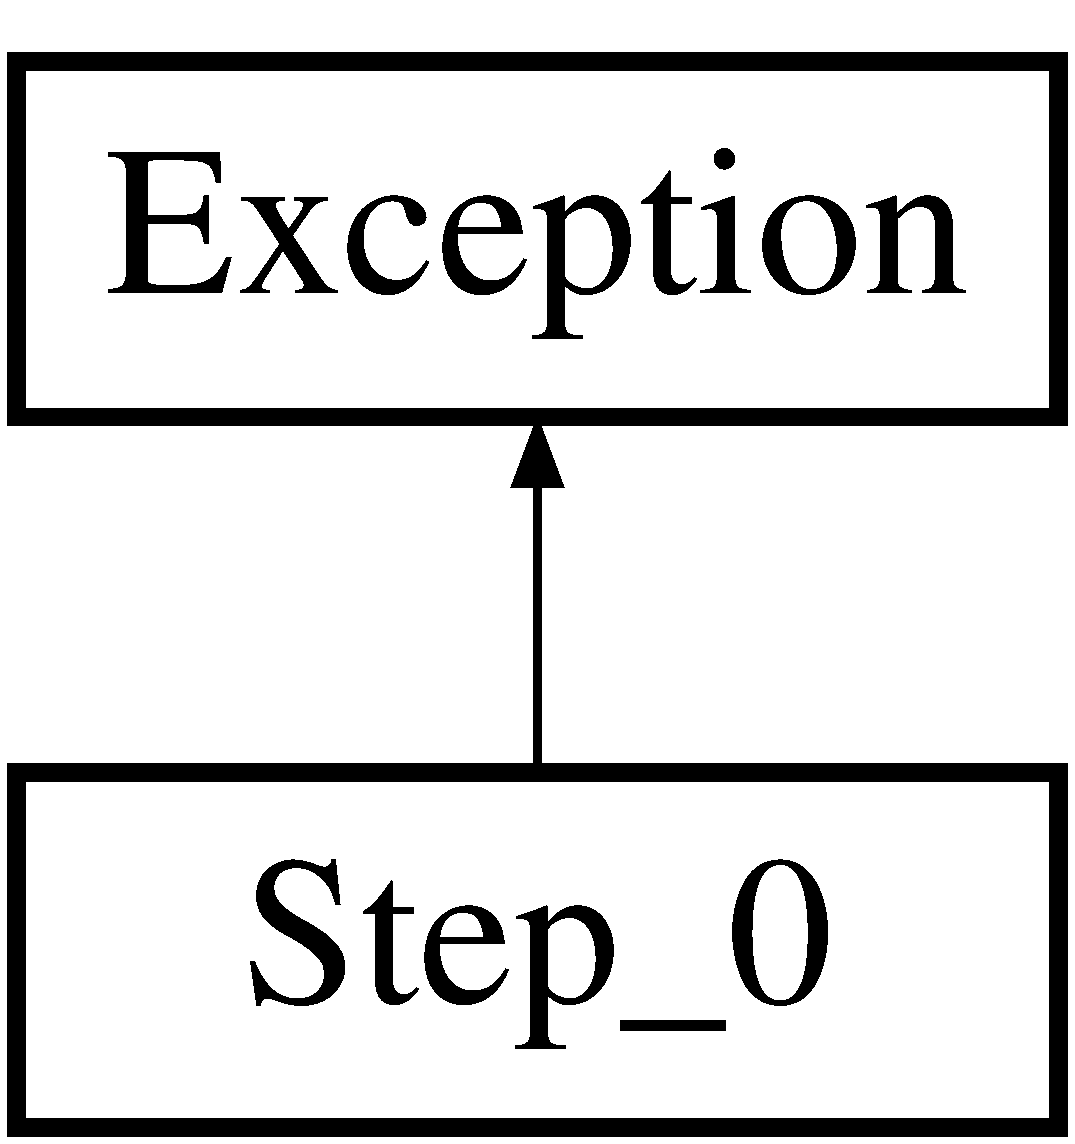
\includegraphics[height=2.000000cm]{classopenbu_1_1sequence_1_1_step__0}
\end{center}
\end{figure}


\subsection{Detailed Description}
\begin{DoxyVerb}Raise when the user try to access subinterval for the first step\end{DoxyVerb}
 

The documentation for this class was generated from the following file\+:\begin{DoxyCompactItemize}
\item 
/\+Users/mouginot/work/app/\+Open\+B\+U/openbu/sequence.\+py\end{DoxyCompactItemize}

\hypertarget{classopenbu_1_1couple_1_1couple__openmc_1_1_s_t_o_p}{}\section{S\+T\+OP Class Reference}
\label{classopenbu_1_1couple_1_1couple__openmc_1_1_s_t_o_p}\index{S\+T\+OP@{S\+T\+OP}}
Inheritance diagram for S\+T\+OP\+:\begin{figure}[H]
\begin{center}
\leavevmode
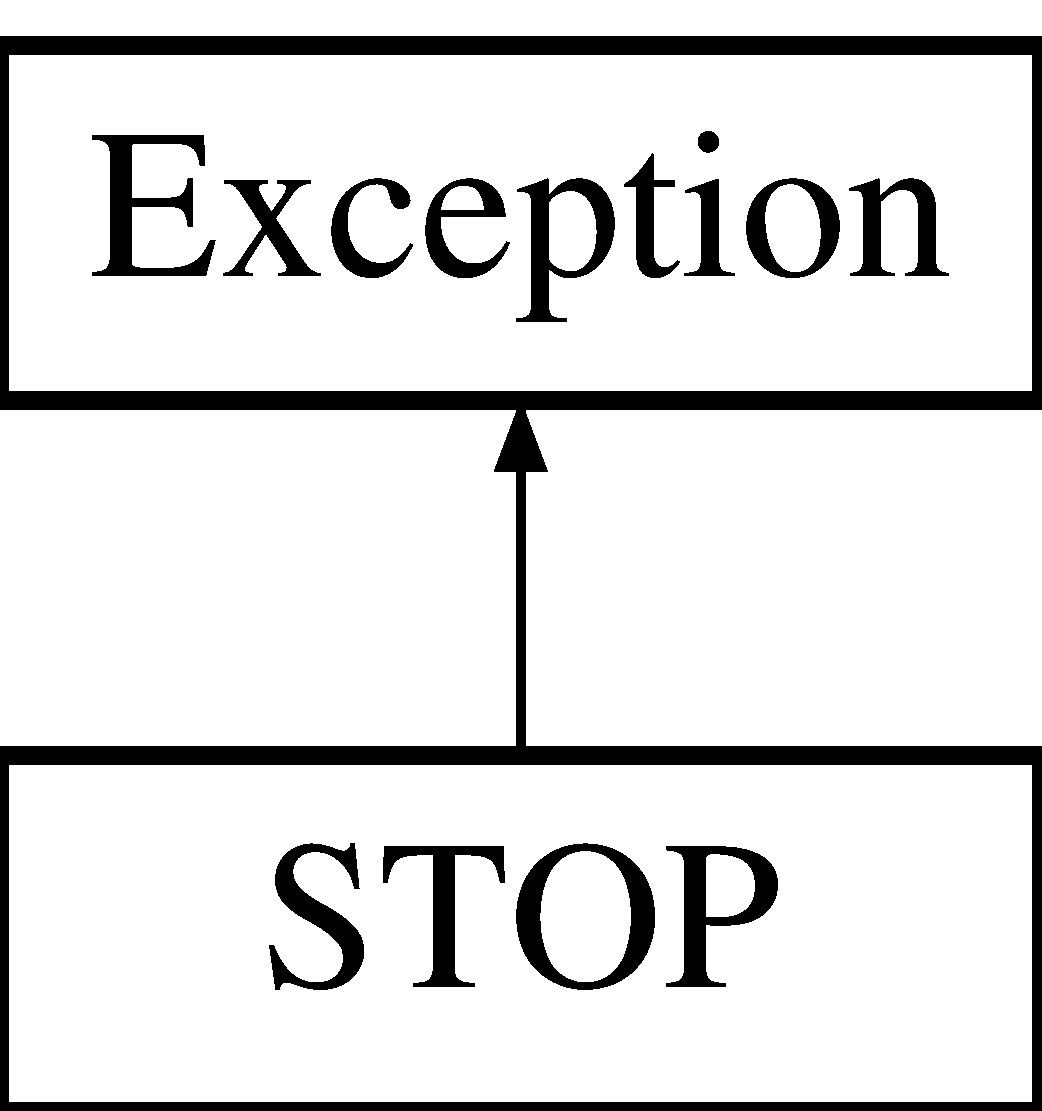
\includegraphics[height=2.000000cm]{classopenbu_1_1couple_1_1couple__openmc_1_1_s_t_o_p}
\end{center}
\end{figure}


\subsection{Detailed Description}
\begin{DoxyVerb}Just a way to stop the code\end{DoxyVerb}
 

The documentation for this class was generated from the following file\+:\begin{DoxyCompactItemize}
\item 
/\+Users/mouginot/work/app/\+Open\+B\+U/openbu/couple/\mbox{\hyperlink{couple__openmc_8py}{couple\+\_\+openmc.\+py}}\end{DoxyCompactItemize}

\hypertarget{classopenbu_1_1system_1_1_system}{}\section{System Class Reference}
\label{classopenbu_1_1system_1_1_system}\index{System@{System}}
Inheritance diagram for System\+:\begin{figure}[H]
\begin{center}
\leavevmode
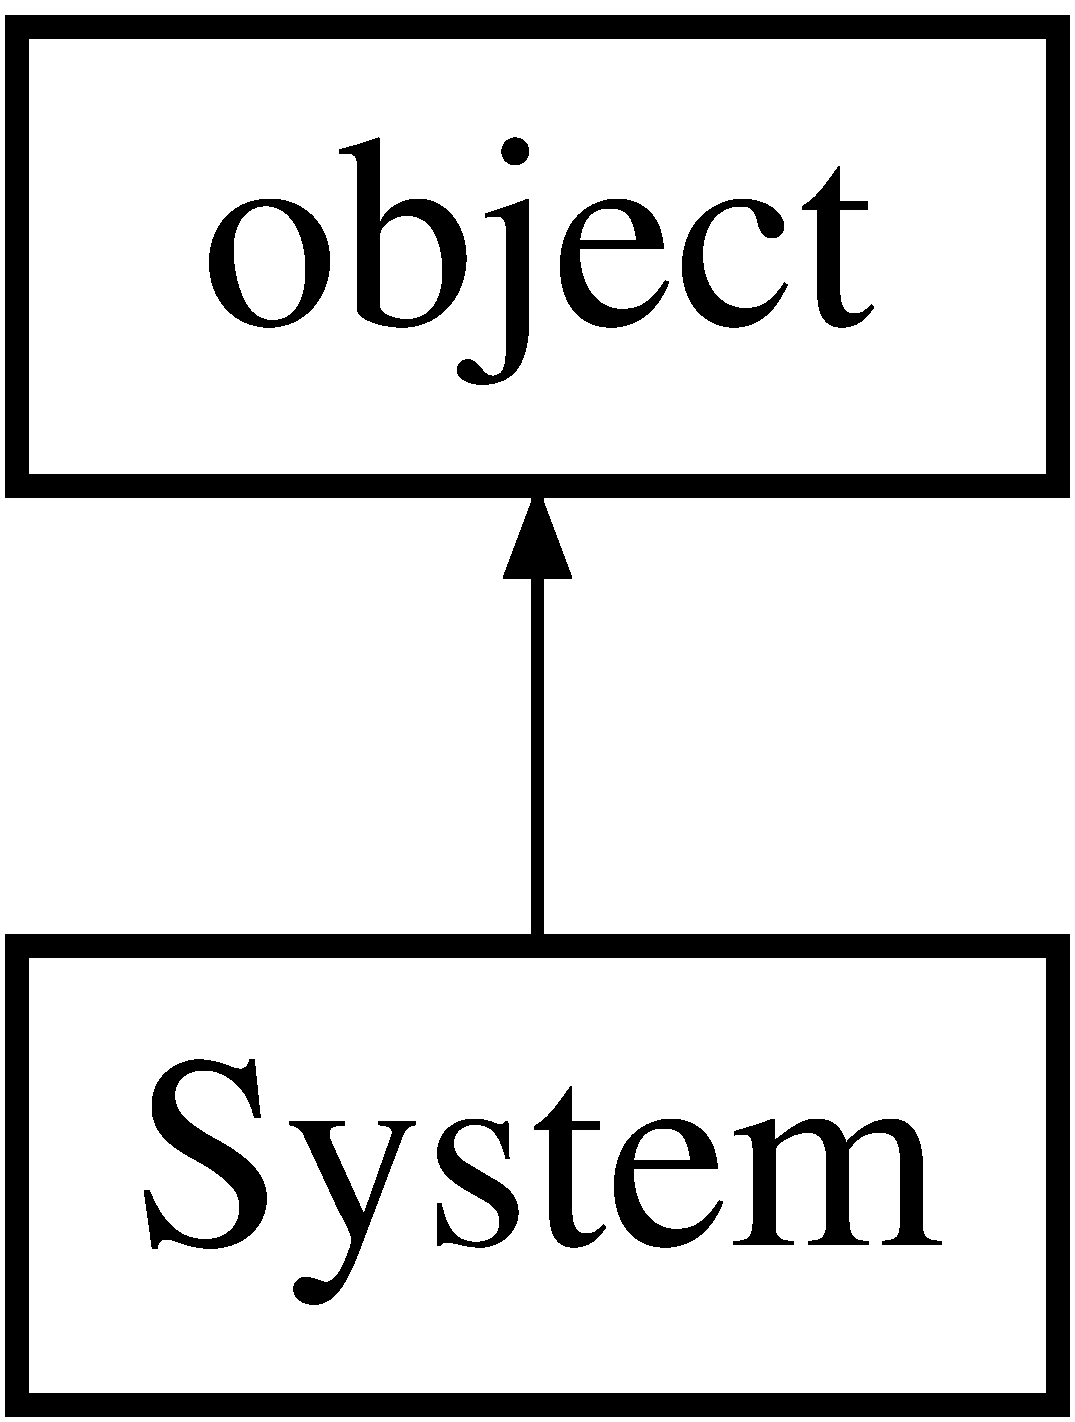
\includegraphics[height=2.000000cm]{classopenbu_1_1system_1_1_system}
\end{center}
\end{figure}
\subsection*{Public Member Functions}
\subsection*{Public Attributes}
\subsection*{Private Member Functions}
\subsection*{Private Attributes}


The documentation for this class was generated from the following file\+:\begin{DoxyCompactItemize}
\item 
/\+Users/mouginot/work/app/\+Open\+B\+U/openbu/system.\+py\end{DoxyCompactItemize}

\hypertarget{classopenbu_1_1utils_1_1reactions__class_1_1xs__lib}{}\section{xs\+\_\+lib Class Reference}
\label{classopenbu_1_1utils_1_1reactions__class_1_1xs__lib}\index{xs\+\_\+lib@{xs\+\_\+lib}}
Inheritance diagram for xs\+\_\+lib\+:\begin{figure}[H]
\begin{center}
\leavevmode
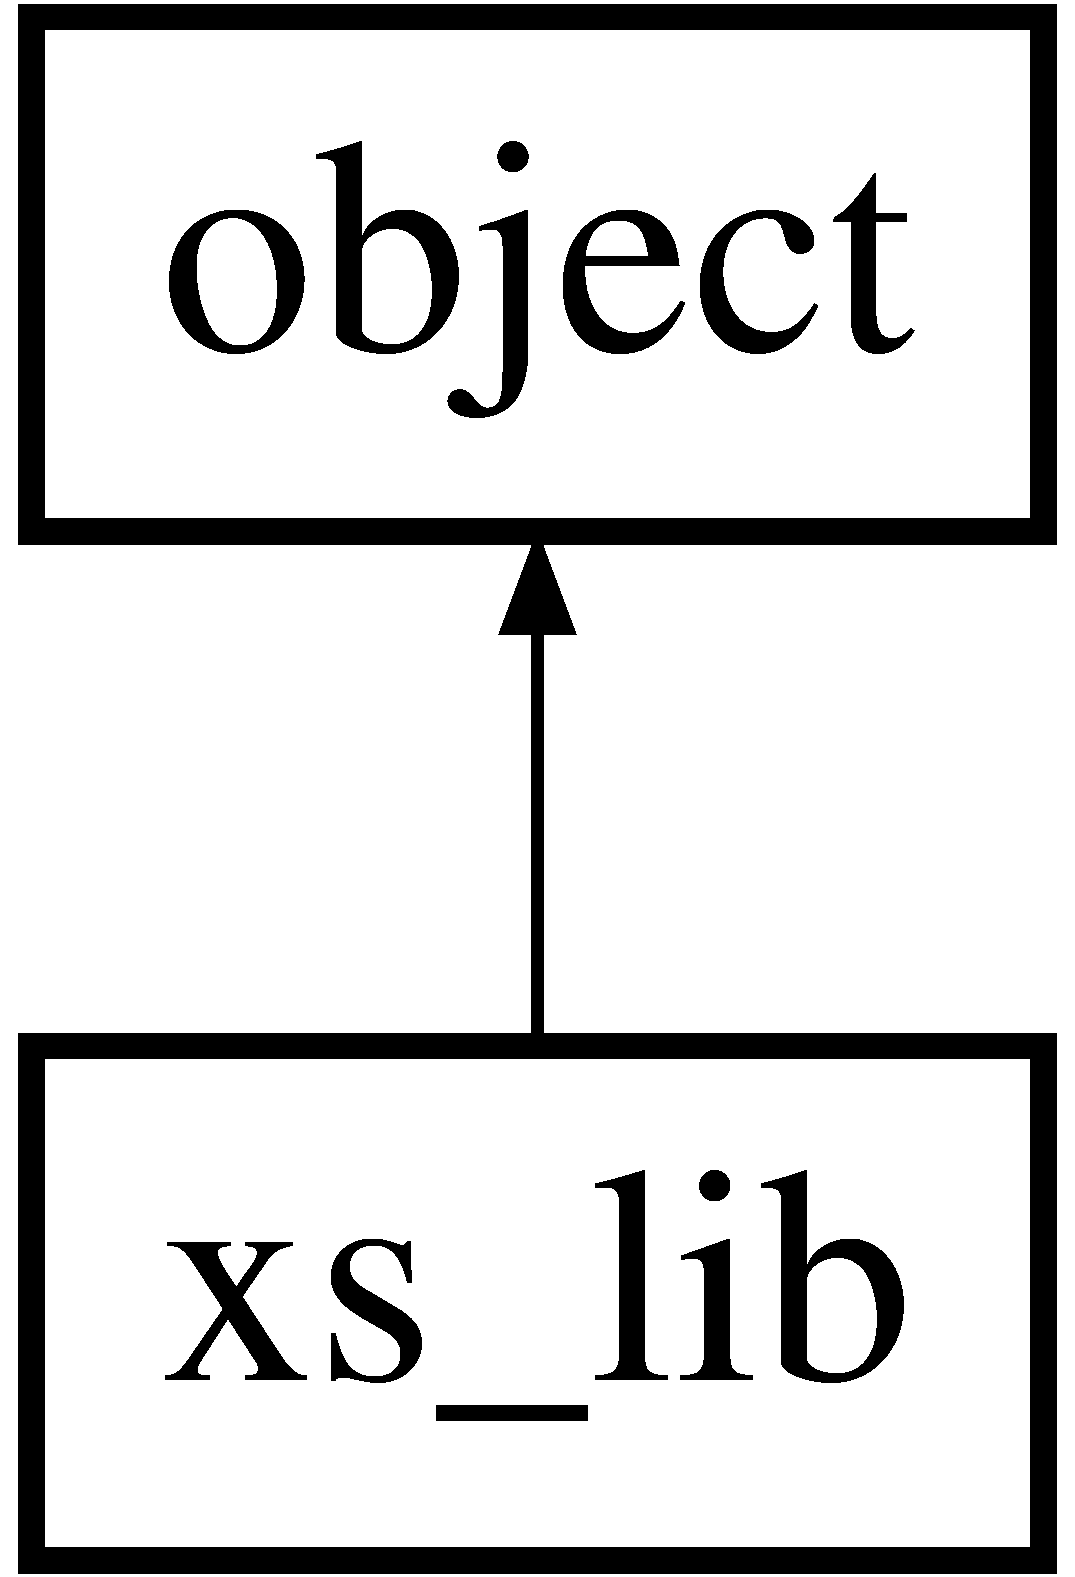
\includegraphics[height=2.000000cm]{classopenbu_1_1utils_1_1reactions__class_1_1xs__lib}
\end{center}
\end{figure}
\subsection*{Public Member Functions}
\subsection*{Private Attributes}


The documentation for this class was generated from the following file\+:\begin{DoxyCompactItemize}
\item 
/\+Users/mouginot/work/app/\+Open\+B\+U/openbu/utils/reactions\+\_\+class.\+py\end{DoxyCompactItemize}

\hypertarget{classopenbu_1_1utils_1_1data__processor_1_1xs__name__not__found}{}\doxysection{xs\+\_\+name\+\_\+not\+\_\+found Class Reference}
\label{classopenbu_1_1utils_1_1data__processor_1_1xs__name__not__found}\index{xs\_name\_not\_found@{xs\_name\_not\_found}}
Inheritance diagram for xs\+\_\+name\+\_\+not\+\_\+found\+:\begin{figure}[H]
\begin{center}
\leavevmode
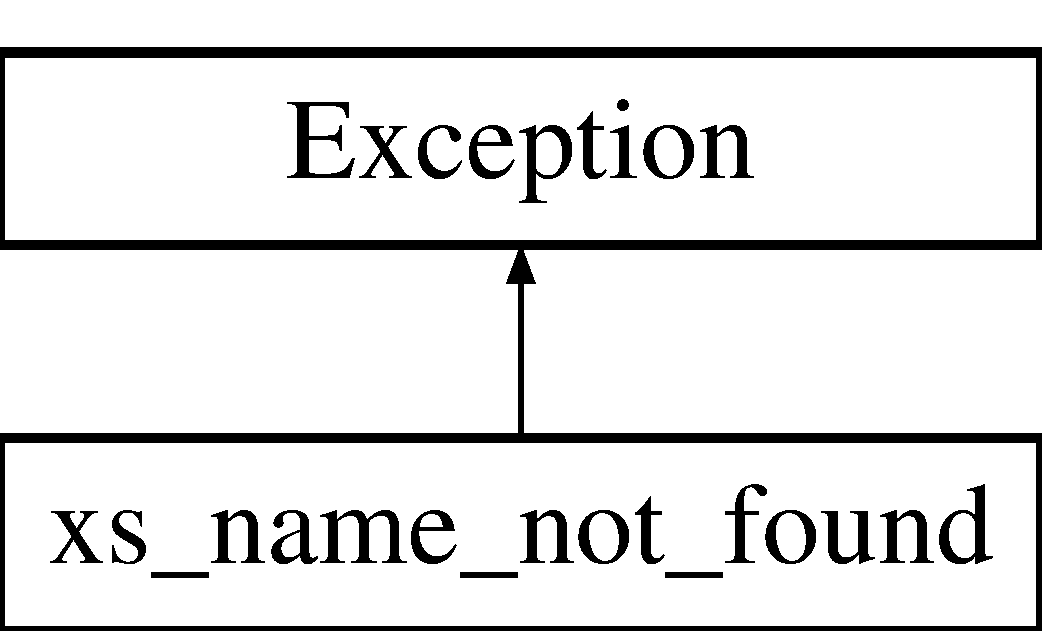
\includegraphics[height=2.000000cm]{classopenbu_1_1utils_1_1data__processor_1_1xs__name__not__found}
\end{center}
\end{figure}


\doxysubsection{Detailed Description}
\begin{DoxyVerb}Raise when the user tries to access fission XS for a nuclide which fission XS have not been set yet \end{DoxyVerb}
 

The documentation for this class was generated from the following file\+:\begin{DoxyCompactItemize}
\item 
utils/data\+\_\+processor.\+py\end{DoxyCompactItemize}

\hypertarget{classopenbu_1_1passport_1_1_x_s__not__yet__set}{}\doxysection{X\+S\+\_\+not\+\_\+yet\+\_\+set Class Reference}
\label{classopenbu_1_1passport_1_1_x_s__not__yet__set}\index{XS\_not\_yet\_set@{XS\_not\_yet\_set}}
Inheritance diagram for X\+S\+\_\+not\+\_\+yet\+\_\+set\+:\begin{figure}[H]
\begin{center}
\leavevmode
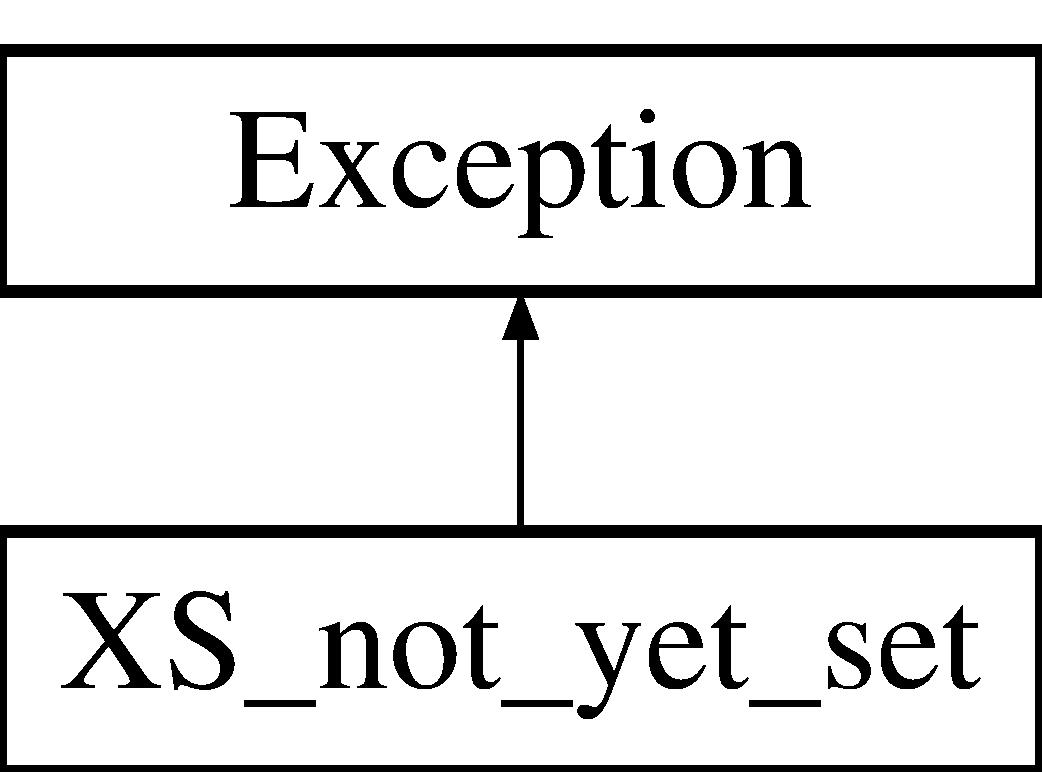
\includegraphics[height=2.000000cm]{classopenbu_1_1passport_1_1_x_s__not__yet__set}
\end{center}
\end{figure}


\doxysubsection{Detailed Description}
\begin{DoxyVerb}Raise when the user tries to access XS for a nuclide which XS have not been set yet \end{DoxyVerb}
 

The documentation for this class was generated from the following file\+:\begin{DoxyCompactItemize}
\item 
passport.\+py\end{DoxyCompactItemize}

\chapter{File Documentation}
\hypertarget{____init_____8py}{}\section{/\+Users/mouginot/work/app/\+Open\+B\+U/openbu/\+\_\+\+\_\+init\+\_\+\+\_\+.py File Reference}
\label{____init_____8py}\index{/\+Users/mouginot/work/app/\+Open\+B\+U/openbu/\+\_\+\+\_\+init\+\_\+\+\_\+.\+py@{/\+Users/mouginot/work/app/\+Open\+B\+U/openbu/\+\_\+\+\_\+init\+\_\+\+\_\+.\+py}}

\hypertarget{couple_2____init_____8py}{}\section{/\+Users/mouginot/work/app/\+Open\+B\+U/openbu/couple/\+\_\+\+\_\+init\+\_\+\+\_\+.py File Reference}
\label{couple_2____init_____8py}\index{/\+Users/mouginot/work/app/\+Open\+B\+U/openbu/couple/\+\_\+\+\_\+init\+\_\+\+\_\+.\+py@{/\+Users/mouginot/work/app/\+Open\+B\+U/openbu/couple/\+\_\+\+\_\+init\+\_\+\+\_\+.\+py}}

\hypertarget{data_2____init_____8py}{}\section{/\+Users/mouginot/work/app/\+Open\+B\+U/openbu/data/\+\_\+\+\_\+init\+\_\+\+\_\+.py File Reference}
\label{data_2____init_____8py}\index{/\+Users/mouginot/work/app/\+Open\+B\+U/openbu/data/\+\_\+\+\_\+init\+\_\+\+\_\+.\+py@{/\+Users/mouginot/work/app/\+Open\+B\+U/openbu/data/\+\_\+\+\_\+init\+\_\+\+\_\+.\+py}}

\hypertarget{nax_2____init_____8py}{}\section{/\+Users/mouginot/work/app/\+Open\+B\+U/openbu/nax/\+\_\+\+\_\+init\+\_\+\+\_\+.py File Reference}
\label{nax_2____init_____8py}\index{/\+Users/mouginot/work/app/\+Open\+B\+U/openbu/nax/\+\_\+\+\_\+init\+\_\+\+\_\+.\+py@{/\+Users/mouginot/work/app/\+Open\+B\+U/openbu/nax/\+\_\+\+\_\+init\+\_\+\+\_\+.\+py}}

\hypertarget{salameche_2____init_____8py}{}\section{/\+Users/mouginot/work/app/\+Open\+B\+U/openbu/salameche/\+\_\+\+\_\+init\+\_\+\+\_\+.py File Reference}
\label{salameche_2____init_____8py}\index{/\+Users/mouginot/work/app/\+Open\+B\+U/openbu/salameche/\+\_\+\+\_\+init\+\_\+\+\_\+.\+py@{/\+Users/mouginot/work/app/\+Open\+B\+U/openbu/salameche/\+\_\+\+\_\+init\+\_\+\+\_\+.\+py}}

\hypertarget{utils_2____init_____8py}{}\section{/\+Users/mouginot/work/app/\+Open\+B\+U/openbu/utils/\+\_\+\+\_\+init\+\_\+\+\_\+.py File Reference}
\label{utils_2____init_____8py}\index{/\+Users/mouginot/work/app/\+Open\+B\+U/openbu/utils/\+\_\+\+\_\+init\+\_\+\+\_\+.\+py@{/\+Users/mouginot/work/app/\+Open\+B\+U/openbu/utils/\+\_\+\+\_\+init\+\_\+\+\_\+.\+py}}

\hypertarget{cell_8py}{}\section{/\+Users/mouginot/work/app/\+Open\+B\+U/openbu/cell.py File Reference}
\label{cell_8py}\index{/\+Users/mouginot/work/app/\+Open\+B\+U/openbu/cell.\+py@{/\+Users/mouginot/work/app/\+Open\+B\+U/openbu/cell.\+py}}
\subsection*{Classes}
\begin{DoxyCompactItemize}
\item 
class \mbox{\hyperlink{classopenbu_1_1cell_1_1_cell}{Cell}}
\item 
class \mbox{\hyperlink{classopenbu_1_1cell_1_1_initial__nucl__not__set}{Initial\+\_\+nucl\+\_\+not\+\_\+set}}
\item 
class \mbox{\hyperlink{classopenbu_1_1cell_1_1_nucl__set__not__in___lib__nucl}{Nucl\+\_\+set\+\_\+not\+\_\+in\+\_\+\+Lib\+\_\+nucl}}
\item 
class \mbox{\hyperlink{classopenbu_1_1cell_1_1_initial__nucl__not__in___nucl__set}{Initial\+\_\+nucl\+\_\+not\+\_\+in\+\_\+\+Nucl\+\_\+set}}
\item 
class \mbox{\hyperlink{classopenbu_1_1cell_1_1_nuclide__list__redundant}{Nuclide\+\_\+list\+\_\+redundant}}
\item 
class \mbox{\hyperlink{classopenbu_1_1cell_1_1_passlist__not__defined}{Passlist\+\_\+not\+\_\+defined}}
\end{DoxyCompactItemize}

\hypertarget{couple__openmc_8py}{}\section{/\+Users/mouginot/work/app/\+Open\+B\+U/openbu/couple/couple\+\_\+openmc.py File Reference}
\label{couple__openmc_8py}\index{/\+Users/mouginot/work/app/\+Open\+B\+U/openbu/couple/couple\+\_\+openmc.\+py@{/\+Users/mouginot/work/app/\+Open\+B\+U/openbu/couple/couple\+\_\+openmc.\+py}}
\subsection*{Classes}
\begin{DoxyCompactItemize}
\item 
class \mbox{\hyperlink{classopenbu_1_1couple_1_1couple__openmc_1_1_couple__openmc}{Couple\+\_\+openmc}}
\item 
class \mbox{\hyperlink{classopenbu_1_1couple_1_1couple__openmc_1_1_initial__nuclides__not__in__nuclide__list}{Initial\+\_\+nuclides\+\_\+not\+\_\+in\+\_\+nuclide\+\_\+list}}
\item 
class \mbox{\hyperlink{classopenbu_1_1couple_1_1couple__openmc_1_1_s_t_o_p}{S\+T\+OP}}
\end{DoxyCompactItemize}

\hypertarget{openmc__fix_8py}{}\section{/\+Users/mouginot/work/app/\+Open\+B\+U/openbu/couple/openmc\+\_\+fix.py File Reference}
\label{openmc__fix_8py}\index{/\+Users/mouginot/work/app/\+Open\+B\+U/openbu/couple/openmc\+\_\+fix.\+py@{/\+Users/mouginot/work/app/\+Open\+B\+U/openbu/couple/openmc\+\_\+fix.\+py}}

\hypertarget{read__energ__grid_8py}{}\section{/\+Users/mouginot/work/app/\+Open\+B\+U/openbu/data/isomeric\+\_\+data/read\+\_\+energ\+\_\+grid.py File Reference}
\label{read__energ__grid_8py}\index{/\+Users/mouginot/work/app/\+Open\+B\+U/openbu/data/isomeric\+\_\+data/read\+\_\+energ\+\_\+grid.\+py@{/\+Users/mouginot/work/app/\+Open\+B\+U/openbu/data/isomeric\+\_\+data/read\+\_\+energ\+\_\+grid.\+py}}

\hypertarget{list__and__dict_8py}{}\section{/\+Users/mouginot/work/app/\+Open\+B\+U/openbu/data/list\+\_\+and\+\_\+dict.py File Reference}
\label{list__and__dict_8py}\index{/\+Users/mouginot/work/app/\+Open\+B\+U/openbu/data/list\+\_\+and\+\_\+dict.\+py@{/\+Users/mouginot/work/app/\+Open\+B\+U/openbu/data/list\+\_\+and\+\_\+dict.\+py}}

\hypertarget{read__fy_8py}{}\section{/\+Users/mouginot/work/app/\+Open\+B\+U/openbu/data/other\+\_\+libs/\+E\+N\+D\+F\+V\+I\+I\+I/read\+\_\+fy.py File Reference}
\label{read__fy_8py}\index{/\+Users/mouginot/work/app/\+Open\+B\+U/openbu/data/other\+\_\+libs/\+E\+N\+D\+F\+V\+I\+I\+I/read\+\_\+fy.\+py@{/\+Users/mouginot/work/app/\+Open\+B\+U/openbu/data/other\+\_\+libs/\+E\+N\+D\+F\+V\+I\+I\+I/read\+\_\+fy.\+py}}

\hypertarget{read__lib__functions_8py}{}\section{/\+Users/mouginot/work/app/\+Open\+B\+U/openbu/data/read\+\_\+lib\+\_\+functions.py File Reference}
\label{read__lib__functions_8py}\index{/\+Users/mouginot/work/app/\+Open\+B\+U/openbu/data/read\+\_\+lib\+\_\+functions.\+py@{/\+Users/mouginot/work/app/\+Open\+B\+U/openbu/data/read\+\_\+lib\+\_\+functions.\+py}}

\hypertarget{build__text__mat_8py}{}\section{/\+Users/mouginot/work/app/\+Open\+B\+U/openbu/data/script/build\+\_\+text\+\_\+mat.py File Reference}
\label{build__text__mat_8py}\index{/\+Users/mouginot/work/app/\+Open\+B\+U/openbu/data/script/build\+\_\+text\+\_\+mat.\+py@{/\+Users/mouginot/work/app/\+Open\+B\+U/openbu/data/script/build\+\_\+text\+\_\+mat.\+py}}

\hypertarget{compare__fy_8py}{}\section{/\+Users/mouginot/work/app/\+Open\+B\+U/openbu/data/script/compare\+\_\+fy.py File Reference}
\label{compare__fy_8py}\index{/\+Users/mouginot/work/app/\+Open\+B\+U/openbu/data/script/compare\+\_\+fy.\+py@{/\+Users/mouginot/work/app/\+Open\+B\+U/openbu/data/script/compare\+\_\+fy.\+py}}

\hypertarget{conv__decaylib_8py}{}\section{/\+Users/mouginot/work/app/\+Open\+B\+U/openbu/data/script/conv\+\_\+decaylib.py File Reference}
\label{conv__decaylib_8py}\index{/\+Users/mouginot/work/app/\+Open\+B\+U/openbu/data/script/conv\+\_\+decaylib.\+py@{/\+Users/mouginot/work/app/\+Open\+B\+U/openbu/data/script/conv\+\_\+decaylib.\+py}}

\hypertarget{conv__fylib_8py}{}\section{/\+Users/mouginot/work/app/\+Open\+B\+U/openbu/data/script/conv\+\_\+fylib.py File Reference}
\label{conv__fylib_8py}\index{/\+Users/mouginot/work/app/\+Open\+B\+U/openbu/data/script/conv\+\_\+fylib.\+py@{/\+Users/mouginot/work/app/\+Open\+B\+U/openbu/data/script/conv\+\_\+fylib.\+py}}

\hypertarget{conv__fylib__janis-csv_8py}{}\section{/\+Users/mouginot/work/app/\+Open\+B\+U/openbu/data/script/conv\+\_\+fylib\+\_\+janis-\/csv.py File Reference}
\label{conv__fylib__janis-csv_8py}\index{/\+Users/mouginot/work/app/\+Open\+B\+U/openbu/data/script/conv\+\_\+fylib\+\_\+janis-\/csv.\+py@{/\+Users/mouginot/work/app/\+Open\+B\+U/openbu/data/script/conv\+\_\+fylib\+\_\+janis-\/csv.\+py}}

\hypertarget{conv__nndc__decaylib_8py}{}\section{/\+Users/mouginot/work/app/\+Open\+B\+U/openbu/data/script/conv\+\_\+nndc\+\_\+decaylib.py File Reference}
\label{conv__nndc__decaylib_8py}\index{/\+Users/mouginot/work/app/\+Open\+B\+U/openbu/data/script/conv\+\_\+nndc\+\_\+decaylib.\+py@{/\+Users/mouginot/work/app/\+Open\+B\+U/openbu/data/script/conv\+\_\+nndc\+\_\+decaylib.\+py}}

\hypertarget{conv__xslib_8py}{}\section{/\+Users/mouginot/work/app/\+Open\+B\+U/openbu/data/script/conv\+\_\+xslib.py File Reference}
\label{conv__xslib_8py}\index{/\+Users/mouginot/work/app/\+Open\+B\+U/openbu/data/script/conv\+\_\+xslib.\+py@{/\+Users/mouginot/work/app/\+Open\+B\+U/openbu/data/script/conv\+\_\+xslib.\+py}}

\hypertarget{convert__decay-old-format__to-new-format_8py}{}\section{/\+Users/mouginot/work/app/\+Open\+B\+U/openbu/data/script/convert\+\_\+decay-\/old-\/format\+\_\+to-\/new-\/format.py File Reference}
\label{convert__decay-old-format__to-new-format_8py}\index{/\+Users/mouginot/work/app/\+Open\+B\+U/openbu/data/script/convert\+\_\+decay-\/old-\/format\+\_\+to-\/new-\/format.\+py@{/\+Users/mouginot/work/app/\+Open\+B\+U/openbu/data/script/convert\+\_\+decay-\/old-\/format\+\_\+to-\/new-\/format.\+py}}

\hypertarget{find__isomeric__branching_8py}{}\section{/\+Users/mouginot/work/app/\+Open\+B\+U/openbu/data/script/find\+\_\+isomeric\+\_\+branching.py File Reference}
\label{find__isomeric__branching_8py}\index{/\+Users/mouginot/work/app/\+Open\+B\+U/openbu/data/script/find\+\_\+isomeric\+\_\+branching.\+py@{/\+Users/mouginot/work/app/\+Open\+B\+U/openbu/data/script/find\+\_\+isomeric\+\_\+branching.\+py}}

\hypertarget{nuclide__chart__compare__fy_8py}{}\section{/\+Users/mouginot/work/app/\+Open\+B\+U/openbu/data/script/nuclide\+\_\+chart\+\_\+compare\+\_\+fy.py File Reference}
\label{nuclide__chart__compare__fy_8py}\index{/\+Users/mouginot/work/app/\+Open\+B\+U/openbu/data/script/nuclide\+\_\+chart\+\_\+compare\+\_\+fy.\+py@{/\+Users/mouginot/work/app/\+Open\+B\+U/openbu/data/script/nuclide\+\_\+chart\+\_\+compare\+\_\+fy.\+py}}

\hypertarget{nuclide__chart__jeff33-32_8py}{}\section{/\+Users/mouginot/work/app/\+Open\+B\+U/openbu/data/script/nuclide\+\_\+chart\+\_\+jeff33-\/32.py File Reference}
\label{nuclide__chart__jeff33-32_8py}\index{/\+Users/mouginot/work/app/\+Open\+B\+U/openbu/data/script/nuclide\+\_\+chart\+\_\+jeff33-\/32.\+py@{/\+Users/mouginot/work/app/\+Open\+B\+U/openbu/data/script/nuclide\+\_\+chart\+\_\+jeff33-\/32.\+py}}

\hypertarget{plot__full__reduced__lib__chart_8py}{}\section{/\+Users/mouginot/work/app/\+Open\+B\+U/openbu/data/script/plot\+\_\+full\+\_\+reduced\+\_\+lib\+\_\+chart.py File Reference}
\label{plot__full__reduced__lib__chart_8py}\index{/\+Users/mouginot/work/app/\+Open\+B\+U/openbu/data/script/plot\+\_\+full\+\_\+reduced\+\_\+lib\+\_\+chart.\+py@{/\+Users/mouginot/work/app/\+Open\+B\+U/openbu/data/script/plot\+\_\+full\+\_\+reduced\+\_\+lib\+\_\+chart.\+py}}

\hypertarget{xs__flux__folder_8py}{}\section{/\+Users/mouginot/work/app/\+Open\+B\+U/openbu/data/script/xs\+\_\+flux\+\_\+folder.py File Reference}
\label{xs__flux__folder_8py}\index{/\+Users/mouginot/work/app/\+Open\+B\+U/openbu/data/script/xs\+\_\+flux\+\_\+folder.\+py@{/\+Users/mouginot/work/app/\+Open\+B\+U/openbu/data/script/xs\+\_\+flux\+\_\+folder.\+py}}

\hypertarget{input_8py}{}\section{/\+Users/mouginot/work/app/\+Open\+B\+U/openbu/input.py File Reference}
\label{input_8py}\index{/\+Users/mouginot/work/app/\+Open\+B\+U/openbu/input.\+py@{/\+Users/mouginot/work/app/\+Open\+B\+U/openbu/input.\+py}}
\subsection*{Classes}
\begin{DoxyCompactItemize}
\item 
class \mbox{\hyperlink{classopenbu_1_1input_1_1_input}{Input}}
\end{DoxyCompactItemize}

\hypertarget{nax_2functions_8py}{}\section{/\+Users/mouginot/work/app/\+Open\+B\+U/openbu/nax/functions.py File Reference}
\label{nax_2functions_8py}\index{/\+Users/mouginot/work/app/\+Open\+B\+U/openbu/nax/functions.\+py@{/\+Users/mouginot/work/app/\+Open\+B\+U/openbu/nax/functions.\+py}}
\subsection*{Classes}
\begin{DoxyCompactItemize}
\item 
class \mbox{\hyperlink{classopenbu_1_1nax_1_1functions_1_1_batch}{Batch}}
\end{DoxyCompactItemize}

\hypertarget{utils_2functions_8py}{}\section{/\+Users/mouginot/work/app/\+Open\+B\+U/openbu/utils/functions.py File Reference}
\label{utils_2functions_8py}\index{/\+Users/mouginot/work/app/\+Open\+B\+U/openbu/utils/functions.\+py@{/\+Users/mouginot/work/app/\+Open\+B\+U/openbu/utils/functions.\+py}}
\subsection*{Classes}
\begin{DoxyCompactItemize}
\item 
class \mbox{\hyperlink{classopenbu_1_1utils_1_1functions_1_1_midpoint_normalize}{Midpoint\+Normalize}}
\item 
class \mbox{\hyperlink{classopenbu_1_1utils_1_1functions_1_1_empty__argument}{Empty\+\_\+argument}}
\end{DoxyCompactItemize}

\hypertarget{passlist_8py}{}\section{/\+Users/mouginot/work/app/\+Open\+B\+U/openbu/passlist.py File Reference}
\label{passlist_8py}\index{/\+Users/mouginot/work/app/\+Open\+B\+U/openbu/passlist.\+py@{/\+Users/mouginot/work/app/\+Open\+B\+U/openbu/passlist.\+py}}
\subsection*{Classes}
\begin{DoxyCompactItemize}
\item 
class \mbox{\hyperlink{classopenbu_1_1passlist_1_1_passlist}{Passlist}}
\item 
class \mbox{\hyperlink{classopenbu_1_1passlist_1_1_nuc__xs__not__found}{Nuc\+\_\+xs\+\_\+not\+\_\+found}}
\item 
class \mbox{\hyperlink{classopenbu_1_1passlist_1_1_neg__decay}{Neg\+\_\+decay}}
\item 
class \mbox{\hyperlink{classopenbu_1_1passlist_1_1_neg__xs}{Neg\+\_\+xs}}
\end{DoxyCompactItemize}

\hypertarget{passport_8py}{}\section{/\+Users/mouginot/work/app/\+Open\+B\+U/openbu/passport.py File Reference}
\label{passport_8py}\index{/\+Users/mouginot/work/app/\+Open\+B\+U/openbu/passport.\+py@{/\+Users/mouginot/work/app/\+Open\+B\+U/openbu/passport.\+py}}
\subsection*{Classes}
\begin{DoxyCompactItemize}
\item 
class \mbox{\hyperlink{classopenbu_1_1passport_1_1_passport}{Passport}}
\item 
class \mbox{\hyperlink{classopenbu_1_1passport_1_1_incorrect__nuc__id}{Incorrect\+\_\+nuc\+\_\+id}}
\item 
class \mbox{\hyperlink{classopenbu_1_1passport_1_1_nuc__xs__not__found}{Nuc\+\_\+xs\+\_\+not\+\_\+found}}
\item 
class \mbox{\hyperlink{classopenbu_1_1passport_1_1_not__a___fission___product}{Not\+\_\+a\+\_\+\+Fission\+\_\+\+Product}}
\item 
class \mbox{\hyperlink{classopenbu_1_1passport_1_1_x_s__not__yet__set}{X\+S\+\_\+not\+\_\+yet\+\_\+set}}
\item 
class \mbox{\hyperlink{classopenbu_1_1passport_1_1_no__fission___x_s}{No\+\_\+fission\+\_\+\+XS}}
\end{DoxyCompactItemize}

\hypertarget{burn_8py}{}\section{/\+Users/mouginot/work/app/\+Open\+B\+U/openbu/salameche/burn.py File Reference}
\label{burn_8py}\index{/\+Users/mouginot/work/app/\+Open\+B\+U/openbu/salameche/burn.\+py@{/\+Users/mouginot/work/app/\+Open\+B\+U/openbu/salameche/burn.\+py}}

\hypertarget{cram_8py}{}\section{/\+Users/mouginot/work/app/\+Open\+B\+U/openbu/salameche/cram.py File Reference}
\label{cram_8py}\index{/\+Users/mouginot/work/app/\+Open\+B\+U/openbu/salameche/cram.\+py@{/\+Users/mouginot/work/app/\+Open\+B\+U/openbu/salameche/cram.\+py}}

\hypertarget{mat__builder_8py}{}\section{/\+Users/mouginot/work/app/\+Open\+B\+U/openbu/salameche/mat\+\_\+builder.py File Reference}
\label{mat__builder_8py}\index{/\+Users/mouginot/work/app/\+Open\+B\+U/openbu/salameche/mat\+\_\+builder.\+py@{/\+Users/mouginot/work/app/\+Open\+B\+U/openbu/salameche/mat\+\_\+builder.\+py}}

\hypertarget{py__pade_8py}{}\section{/\+Users/mouginot/work/app/\+Open\+B\+U/openbu/salameche/py\+\_\+pade.py File Reference}
\label{py__pade_8py}\index{/\+Users/mouginot/work/app/\+Open\+B\+U/openbu/salameche/py\+\_\+pade.\+py@{/\+Users/mouginot/work/app/\+Open\+B\+U/openbu/salameche/py\+\_\+pade.\+py}}

\hypertarget{sequence_8py}{}\section{/\+Users/mouginot/work/app/\+Open\+B\+U/openbu/sequence.py File Reference}
\label{sequence_8py}\index{/\+Users/mouginot/work/app/\+Open\+B\+U/openbu/sequence.\+py@{/\+Users/mouginot/work/app/\+Open\+B\+U/openbu/sequence.\+py}}
\subsection*{Classes}
\begin{DoxyCompactItemize}
\item 
class \mbox{\hyperlink{classopenbu_1_1sequence_1_1_sequence}{Sequence}}
\item 
class \mbox{\hyperlink{classopenbu_1_1sequence_1_1_step__0}{Step\+\_\+0}}
\end{DoxyCompactItemize}

\hypertarget{standalone_8py}{}\section{/\+Users/mouginot/work/app/\+Open\+B\+U/openbu/standalone.py File Reference}
\label{standalone_8py}\index{/\+Users/mouginot/work/app/\+Open\+B\+U/openbu/standalone.\+py@{/\+Users/mouginot/work/app/\+Open\+B\+U/openbu/standalone.\+py}}
\subsection*{Classes}
\begin{DoxyCompactItemize}
\item 
class \mbox{\hyperlink{classopenbu_1_1standalone_1_1_stand__alone}{Stand\+\_\+alone}}
\end{DoxyCompactItemize}

\hypertarget{system_8py}{}\section{/\+Users/mouginot/work/app/\+Open\+B\+U/openbu/system.py File Reference}
\label{system_8py}\index{/\+Users/mouginot/work/app/\+Open\+B\+U/openbu/system.\+py@{/\+Users/mouginot/work/app/\+Open\+B\+U/openbu/system.\+py}}
\subsection*{Classes}
\begin{DoxyCompactItemize}
\item 
class \mbox{\hyperlink{classopenbu_1_1system_1_1_system}{System}}
\item 
class \mbox{\hyperlink{classopenbu_1_1system_1_1_cell__name__not__found}{Cell\+\_\+name\+\_\+not\+\_\+found}}
\end{DoxyCompactItemize}

\hypertarget{data__processor_8py}{}\section{/\+Users/mouginot/work/app/\+Open\+B\+U/openbu/utils/data\+\_\+processor.py File Reference}
\label{data__processor_8py}\index{/\+Users/mouginot/work/app/\+Open\+B\+U/openbu/utils/data\+\_\+processor.\+py@{/\+Users/mouginot/work/app/\+Open\+B\+U/openbu/utils/data\+\_\+processor.\+py}}
\subsection*{Classes}
\begin{DoxyCompactItemize}
\item 
class \mbox{\hyperlink{classopenbu_1_1utils_1_1data__processor_1_1xs__name__not__found}{xs\+\_\+name\+\_\+not\+\_\+found}}
\end{DoxyCompactItemize}

\hypertarget{printer_8py}{}\section{/\+Users/mouginot/work/app/\+Open\+B\+U/openbu/utils/printer.py File Reference}
\label{printer_8py}\index{/\+Users/mouginot/work/app/\+Open\+B\+U/openbu/utils/printer.\+py@{/\+Users/mouginot/work/app/\+Open\+B\+U/openbu/utils/printer.\+py}}

\hypertarget{reactions__class_8py}{}\section{/\+Users/mouginot/work/app/\+Open\+B\+U/openbu/utils/reactions\+\_\+class.py File Reference}
\label{reactions__class_8py}\index{/\+Users/mouginot/work/app/\+Open\+B\+U/openbu/utils/reactions\+\_\+class.\+py@{/\+Users/mouginot/work/app/\+Open\+B\+U/openbu/utils/reactions\+\_\+class.\+py}}
\subsection*{Classes}
\begin{DoxyCompactItemize}
\item 
class \mbox{\hyperlink{classopenbu_1_1utils_1_1reactions__class_1_1decay__lib}{decay\+\_\+lib}}
\item 
class \mbox{\hyperlink{classopenbu_1_1utils_1_1reactions__class_1_1xs__lib}{xs\+\_\+lib}}
\item 
class \mbox{\hyperlink{classopenbu_1_1utils_1_1reactions__class_1_1fy__lib}{fy\+\_\+lib}}
\item 
class \mbox{\hyperlink{classopenbu_1_1utils_1_1reactions__class_1_1_empty__data}{Empty\+\_\+data}}
\end{DoxyCompactItemize}

%--- End generated contents ---

% Index
\backmatter
\newpage
\phantomsection
\clearemptydoublepage
\addcontentsline{toc}{chapter}{Index}
\printindex

\end{document}
